% chktex-file 2% chktex-file 29
% chktex-file 13
\documentclass{report}
\usepackage{setspace}
\usepackage[a4paper, total={7in, 10in}]{geometry}
\usepackage[fleqn]{amsmath}
\usepackage{empheq}
\usepackage{amssymb}
\usepackage{amsthm}
\usepackage{gensymb}
\usepackage[fleqn]{cases}
\usepackage{multicol}
\usepackage{color}
\usepackage{stix}
\usepackage{chngcntr}
\usepackage{tikz}
\usepackage{enumitem}
\usepackage{pgfplots}
\usepackage{etoolbox}
\usepackage{tikz-3dplot}
\usepackage{tkz-euclide}
\usepackage{graphicx}
\usepackage{enumitem}

\def\nswe#1#2#3{#1\,$#2^\circ\,#3'$}
\graphicspath{ {./assets/} }
\usetikzlibrary{calc,matrix,arrows}
\usetikzlibrary{decorations.pathmorphing,patterns, calligraphy, perspective,backgrounds}

\tikzset{
    right angle quadrant/.code={
            \pgfmathsetmacro\quadranta{{1,1,-1,-1}[#1-1]}     % Arrays for selecting quadrant
            \pgfmathsetmacro\quadrantb{{1,-1,-1,1}[#1-1]}},
    right angle quadrant=1, % Make sure it is set, even if not called explicitly
    right angle length/.code={\def\rightanglelength{#1}},   % Length of symbol
    right angle length=2ex, % Make sure it is set...
    right angle symbol/.style n args={3}{
            insert path={
                    let \p0 = ($(#1)!(#3)!(#2)$) in     % Intersection
                    let \p1 = ($(\p0)!\quadranta*\rightanglelength!(#3)$), % Point on base line
                    \p2 = ($(\p0)!\quadrantb*\rightanglelength!(#2)$) in % Point on perpendicular line
                    let \p3 = ($(\p1)+(\p2)-(\p0)$) in  % Corner point of symbol
                    (\p1) -- (\p3) -- (\p2)
                }
        }
}

\counterwithout{equation}{chapter}
\setlength{\columnseprule}{1pt}
\setlength{\columnsep}{24pt}
\setcounter{chapter}{11}
\hfuzz=100pt

\newcommand{\pgfplotsdrawaxis}{\pgfplots@draw@axis}
\makeatother
\pgfplotsset{only axis on top/.style={axis on top=false, after end axis/.code={
                    \pgfplotsset{axis line style=opaque, ticklabel style=opaque, tick style={thick,opaque},
                        grid=none}\pgfplotsdrawaxis}}}

\newtheorem{theorem}{Theorem}

\begin{document}
\makeatletter
\newcommand{\newparallel}{\mathrel{\mathpalette\new@parallel\relax}}
\newcommand{\new@parallel}[2]{%
    \begingroup
    \sbox\z@{$#1T$}% get the height of an uppercase letter
    \resizebox{!}{\ht\z@}{\raisebox{\depth}{$\m@th#1/\mkern-5mu/$}}%
    \endgroup
}
\makeatother

\newcommand{\planelineinter}[5]% a, b, c, p as {a_x,a_y,a_z}, coordinate name
{   \foreach \a [count=\k] in {#1}
        { \ifthenelse{\k=1}{\xdef\tempxa{\a}}
            \ifthenelse{\k=2}{\xdef\tempya{\a}}
            \ifthenelse{\k=3}{\xdef\tempza{\a}}
        }
    \foreach \b [count=\k] in {#2}
        { \ifthenelse{\k=1}{\xdef\tempxb{\b}}
            \ifthenelse{\k=2}{\xdef\tempyb{\b}}
            \ifthenelse{\k=3}{\xdef\tempzb{\b}}
        }
    \foreach \c [count=\k] in {#3}
        { \ifthenelse{\k=1}{\xdef\tempxc{\c}}
            \ifthenelse{\k=2}{\xdef\tempyc{\c}}
            \ifthenelse{\k=3}{\xdef\tempzc{\c}}
        }
    \foreach \p [count=\k] in {#4}
        { \ifthenelse{\k=1}{\xdef\tempxp{\p}}
            \ifthenelse{\k=2}{\xdef\tempyp{\p}}
            \ifthenelse{\k=3}{\xdef\tempzp{\p}}
        }
    \pgfmathsetmacro{\abx}{\tempxb-\tempxa}
    \pgfmathsetmacro{\aby}{\tempyb-\tempya}
    \pgfmathsetmacro{\abz}{\tempzb-\tempza}
    \pgfmathsetmacro{\acx}{\tempxc-\tempxa}
    \pgfmathsetmacro{\acy}{\tempyc-\tempya}
    \pgfmathsetmacro{\acz}{\tempzc-\tempza}
    \pgfmathsetmacro{\nx}{\aby*\acz-\abz*\acy}
    \pgfmathsetmacro{\ny}{\abz*\acx-\abx*\acz}
    \pgfmathsetmacro{\nz}{\abx*\acy-\aby*\acx}
    \pgfmathsetmacro{\d}{(\nx+\ny+\nz)/(\nx*\tempxp+\ny*\tempyp+\nz*\tempzp)}
    \path (0,0,0) -- (#4) coordinate[pos=\d] (#5);
}

% golden ratio and inverse golden ratio
\pgfmathsetmacro{\gr}{(1+sqrt(5))/2}
\pgfmathsetmacro{\igr}{2/(1+sqrt(5))}

%choose axis angles
\newcommand{\xangle}{0}
\newcommand{\yangle}{90}
\newcommand{\zangle}{225}

%choose axis lengths
\newcommand{\xlength}{1}
\newcommand{\ylength}{1}
\newcommand{\zlength}{0.5}

\pgfmathsetmacro{\xx}{\xlength*cos(\xangle)}
\pgfmathsetmacro{\xy}{\xlength*sin(\xangle)}
\pgfmathsetmacro{\yx}{\ylength*cos(\yangle)}
\pgfmathsetmacro{\yy}{\ylength*sin(\yangle)}
\pgfmathsetmacro{\zx}{\zlength*cos(\zangle)}
\pgfmathsetmacro{\zy}{\zlength*sin(\zangle)}

\newcommand{\sol}[1]{

    \noindent \textbf{Sol.}
}
\newcommand{\prooff}[1]{

    \noindent \textbf{Proof.}
}
\newcommand\m[1]{\begin{pmatrix}#1\end{pmatrix}}
\newcommand\vm[1]{\begin{vmatrix}#1\end{vmatrix}}
\newenvironment{amatrix}[1]{%
    \left(\begin{array}{@{}*{#1}{c}|c@{}}
        }{%
    \end{array}\right)
}
\newenvironment{cequation}{
    \makeatletter
    \setbool{@fleqn}{false}
    \makeatother
    \begin{equation*}
        }{\end{equation*}}

\begin{titlepage}
    \raggedleft{}
    \rule{1pt}{\textheight}
    \hspace{0.02\textwidth}
    \parbox[b]{0.75\textwidth}{

    {\Huge\bfseries Solution Book of \\[0.5\baselineskip] Mathematic}\\[2\baselineskip]
    {\large\textit{Senior 2 Part I}}\\[4\baselineskip]
    {\Large\textsc{MELVIN CHIA}}

    \vspace{0.5\textheight}

    {\noindent Written on 9 October 2022}\\[\baselineskip]
    }

\end{titlepage}

\doublespacing{}
\tableofcontents
\singlespacing{}
\newpage

\begin{multicols}{2}

  \chapter{Sequence and Series}

  \section{Sequence and Series}

  \subsection{Practice 1}

  \begin{enumerate}
    \item Find the first 5 terms of the sequence $a_{n} = \frac{2^{n}}{n+1}$.

          \textbf{sol{}.} $a_{1} = \frac{2}{2}= 1, a_{2} = \frac{4}{3}, a_{3} = \frac{8}{4}
            , a_{4} = \frac{16}{5}, a_{5} = \frac{32}{6}$

    \item Write the general term of the sequence $1, 8, 27, 64, \cdots$

          \textbf{sol{}.} $a_{n} = n^{3}$
  \end{enumerate}

  \subsection{Practice 2}

  \begin{enumerate}
    \item Express the series $\sum_{n=1}^{10}{n^2+1}$ in the form of numbers.

          \begin{flalign*}
            \textbf{sol{}.} & \sum_{n=1}^{10}{n^2+1}                          & \\
                            & = (1^{2}+1) + (2^{2}+1) + (3^{2}+1) + (4^{2}+1)   \\ & + (5^{2}+1) + (6^{2}+1) + (7^{2}+1) \\ & + (8^{2}+1) + (9^{2}+1) + (10^{2}+1) &  \\
                            & = 2 + 5 + 10 + 17 + 26 + 37 + 50 + 65             \\ & + 82 + 101
          \end{flalign*}

    \item Write the first term, last term and the number of terms of the series
          $\sum_{n=1}^{10}{(3^n-2^n)}$.

          \begin{flalign*}
            \textbf{sol{}.} & First\ term = (3^{1}-2^{1}) = 1      & \\
                            & Last\ term = (3^{10}-2^{10}) = 59049 & \\
                            & Number\ of\ terms = 10
          \end{flalign*}

    \item Express the series $2\cdot5 + 3\cdot7 + 4\cdot9 + \cdots + 15\cdot31$ in the
          form of $\sum$.

          \begin{flalign*}
            \noindent \textbf{sol{}.}                                       \\
            a_{1}         & = 2\cdot5 = 10                                  \\
            a_{2}         & = 3\cdot7 = 21                                  \\
            a_{3}         & = 4\cdot9 = 36                                  \\
            a_{4}         & = 5\cdot11 = 55                                 \\
                          & \vdots                                          \\
            a_{15}        & = 15\cdot31 = 465                               \\
            \therefore\ 2 & \cdot5 + 3\cdot7 + 4\cdot9 + \cdots + 15\cdot31 \\ & = \sum_{n=1}^{15}a_{n}
          \end{flalign*}
  \end{enumerate}

  \subsection{Exercise 12.1}
  \begin{enumerate}

    \item Find the general term of the following sequences.

          \begin{enumerate}
            \item 5, 8, 11, 14, \ldots

                  \textbf{sol{}.} $a_{n} = 3n+2$

            \item 2, 4, 8, 16, \ldots

                  \textbf{sol{}.} $a_{n} = 2^{n}$

            \item $\frac{2}{1}, \frac{3}{2}, \frac{4}{3}, \frac{5}{4}, \cdots$

                  \textbf{sol{}.} $a_{n} = \frac{n+1}{n}$

            \item $\frac{2}{5}, \frac{4}{7}, \frac{6}{9}, \frac{8}{11}, \cdots$

                  \textbf{sol{}.} $a_{n} = \frac{2n}{2n+1}$
          \end{enumerate}

    \item Find the first 5 terms of the following sequences.

          \begin{enumerate}
            \item $a_{n} = 2n+3$

                  \textbf{sol{}.}
                  $a_{1} = 2\cdot1+3 = 5, a_{2} = 2\cdot2+3 = 7, a_{3} = 2\cdot3+3 = 9, a_{4}
                    = 2\cdot4+3 = 11, a_{5} = 2\cdot5+3 = 13$

            \item $a_{n} = n(n-2)$

                  \textbf{sol{}.}
                  $a_{1} = 1\cdot(-1) = -1, a_{2} = 2\cdot0 = 0, a_{3} = 3\cdot1 = 3, a_{4}
                    = 4\cdot2 = 8, a_{5} = 5\cdot3 = 15$

            \item $a_{n} = \frac{n}{2n+1}$

                  \textbf{sol{}.}
                  $a_{1} = \frac{1}{2\cdot1+1}= \frac{1}{3}, a_{2} = \frac{2}{2\cdot2+1}= \frac{2}{5}
                    , a_{3} = \frac{3}{2\cdot3+1}= \frac{3}{7}, a_{4} = \frac{4}{2\cdot4+1}=
                    \frac{4}{9}, a_{5} = \frac{5}{2\cdot5+1}= \frac{5}{11}$

            \item $a_{n} = {{(-3)}}^{n}$

                  \textbf{sol{}.}
                  $a_{1} = {(-3)}^{1} = -3, a_{2} = {(-3)}^{2} = 9, a_{3} = {(-3)}^{3} = -27, a_{4}
                      = {(-3)}^{4} = 81, a_{5} = {(-3)}^{5} = -243$
          \end{enumerate}

    \item Express the following series in the form of numbers.

          \begin{enumerate}
            \item $\sum_{n=1}^{5}{n(n+3)}$

                  \begin{flalign*}
                    \textbf{sol{}.} & \sum_{n=1}^{5}{n(n+3)}                          & \\
                                    & = (1\cdot4) + (2\cdot5) + (3\cdot6) + (4\cdot7)   \\ & + (5\cdot8) &  \\
                                    & = 4 + 10 + 18 + 28 + 40                         & \\
                  \end{flalign*}

            \item $\sum_{n=2}^{6}{\frac{1}{3^{n}}}$

                  \begin{flalign*}
                    \textbf{sol{}.} & \sum_{n=2}^{6}{\frac{1}{3^{n}}}                                                       & \\
                                    & = \frac{1}{3^{2}}+ \frac{1}{3^{3}}+ \frac{1}{3^{4}}+ \frac{1}{3^{5}}+ \frac{1}{3^{6}} & \\
                                    & = \frac{1}{9}+ \frac{1}{27}+ \frac{1}{81}+ \frac{1}{243}+ \frac{1}{729}
                  \end{flalign*}

            \item $\sum_{n=1}^{6}{\frac{1}{n(2n+1)}}$

                  \begin{flalign*}
                    \textbf{sol{}.} & \sum_{n=1}^{6}{\frac{1}{n(2n+1)}}                                                   & \\
                                    & = \frac{1}{1(2\cdot1+1)}+ \frac{1}{2(2\cdot2+1)}                                      \\                                                                                                                                                                                                                                                                                                                                                                                                                                                                                                                                                                                                                                                                                                                                                                                                                                          & + \frac{1}{3(2\cdot3+1)} +
                    \frac{1}{4(2\cdot4+1)}                                                                                  \\ &+ \frac{1}{5(2\cdot5+1)}+ \frac{1}{6(2\cdot6+1)}        &  \\
                                    & = \frac{1}{3}+ \frac{1}{10}+ \frac{1}{21}+ \frac{1}{36}+ \frac{1}{55}+ \frac{1}{78}
                  \end{flalign*}

            \item $\sum_{n=2}^{5}{\frac{1}{n^{2}+2}}$

                  \begin{flalign*}
                    \textbf{sol{}.} & \sum_{n=2}^{5}{\frac{1}{n^{2}+2}}                              & \\
                                    & = \frac{1}{4+2}+ \frac{1}{9+2}+ \frac{1}{16+2}+ \frac{1}{25+2} & \\
                                    & = \frac{1}{6}+ \frac{1}{11}+ \frac{1}{18}+ \frac{1}{27}
                  \end{flalign*}

          \end{enumerate}

    \item Find the first term, last term and the number of terms of the following series.

          \begin{enumerate}
            \item $\sum_{n=3}^{10}{2^2}$

                  \textbf{sol{}.} $a_{3} = 2^{2} = 4, a_{10}= 2^{2} = 4, n = 10-3+1 = 8$

            \item $\sum_{n=1}^{8}{\frac{n+2}{n}}$

                  \textbf{sol{}.}
                  $a_{1} = \frac{1+2}{1}= \frac{3}{1}= 3, a_{8}= \frac{8+2}{8}= \frac{10}{8}
                    = \frac{5}{4}, n = 8-1+1 = 8$

            \item $\sum_{n=1}^{10}{3n^2-n}$

                  \textbf{sol{}.}
                  $a_{1} = 3\cdot1^{2}-1 = 2, a_{10}= 3\cdot10^{2}-10 = 290, n = 10-1+1
                    = 10$

            \item $\sum_{n=9}^{14}{n^2(n-7)}$

                  \textbf{sol{}.}
                  $a_{9} = 9^{2}(9-7) = 9^{2}\cdot2 = 162, a_{14}= 14^{2}(14-7) = 14^{2}
                    \cdot7 = 2744, n = 14-9+1 = 6$
          \end{enumerate}

    \item Express the following series in the form of $\sum$.

          \begin{enumerate}
            \item $1+\frac{1}{2}+\frac{1}{3}+\cdots+\frac{1}{30}$
                  \sol{}
                  \begin{flalign*}
                    a_{1}         & = 1                                                                        \\
                    a_{2}         & = \frac{1}{2}                                                              \\
                    a_{3}         & = \frac{1}{3}                                                              \\
                    \vdots                                                                                     \\
                    a_{30}        & = \frac{1}{30}                                                             \\
                    \therefore\ 1 & +\frac{1}{2}+\frac{1}{3}+\cdots+\frac{1}{30}= \sum_{n=1}^{30}{\frac{1}{n}}
                  \end{flalign*}

            \item $1^{3} + 2^{3} + 3^{3} + \cdots + 50^{3}$
                  \sol{}
                  \begin{flalign*}
                    a_{1}             & = 1^{3}                                                  \\
                    a_{2}             & = 2^{3}                                                  \\
                    a_{3}             & = 3^{3}                                                  \\
                    \vdots                                                                       \\
                    a_{50}            & = 50^{3}                                                 \\
                    \therefore\ 1^{3} & + 2^{3} + 3^{3} + \cdots + 50^{3} = \sum_{n=1}^{50}{n^3}
                  \end{flalign*}

            \item $1  - \frac{1}{2}+ \frac{1}{4}- \frac{1}{8}+ \frac{1}{16}$
                  \sol{}
                  \begin{flalign*}
                    a_{1}         & = {(-\frac{1}{2})}^{1-1}                              \\
                    a_{2}         & = {(-\frac{1}{2})}^{2-1}                              \\
                    a_{3}         & = {(-\frac{1}{2})}^{3-1}                              \\
                    a_{4}         & = {(-\frac{1}{2})}^{4-1}                              \\
                    a_{5}         & = {(-\frac{1}{2})}^{5-1}                              \\
                    \therefore\ 1 & - \frac{1}{2}+ \frac{1}{4}- \frac{1}{8}+ \frac{1}{16} \\ & = \sum_{n=1}^{5}{{(-\frac{1}{2})}^{n-1}}
                  \end{flalign*}

            \item $2\cdot4 + 4\cdot7 + 6\cdot10 + 8\cdot13 + 10\cdot16$
                  \sol{}
                  \begin{flalign*}
                    a_{1}         & = 2\cdot1\cdot(3\cdot1+1)              \\
                    a_{2}         & = 2\cdot2\cdot(3\cdot2+1)              \\
                    a_{3}         & = 2\cdot3\cdot(3\cdot3+1)              \\
                    a_{4}         & = 2\cdot4\cdot(3\cdot4+1)              \\
                    a_{5}         & = 2\cdot5\cdot(3\cdot5+1)              \\
                    \therefore\ 2 & \cdot4 + 4\cdot7 + 6\cdot10 + 8\cdot13 \\ & + 10\cdot16 = \sum_{n=1}^{5}{2n(3n+1)}
                  \end{flalign*}
          \end{enumerate}
  \end{enumerate}

  \section{Arithmetic Progression}

  General term of an Arithmetic Progression (AP) is given by
  \begin{cequation}
    a_{n} = a_{1} + (n-1)d
  \end{cequation}
  where $a_{1}$ is the first term, $d$ is the common difference and $n$ is the
  number of terms.

  \subsection{Practice 3}

  \begin{enumerate}
    \item Find the number of terms of the AP $-4 - 2\frac{3}{4}- 1\frac{1}{2}-
            \frac{1}{4} + \cdots + 16$.

          \begin{flalign*}
            a_{1} & = -4                    \\
            a_{n} & = 16                    \\
            d     & = -2\frac{3}{4}- (-4)   \\
                  & = -2\frac{3}{4}+ 4      \\
                  & = \frac{5}{4}           \\
            16    & = -4 + (n-1)\frac{5}{4} \\
            20    & = \frac{5}{4}(n-1)      \\
            80    & = 5(n-1)                \\
            n-1   & = 16                    \\
            n     & = 17
          \end{flalign*}

    \item Given that $a_{2} = 4$ and $a_{6} = -8$, find the 10th term of the AP. \sol{}
          \begin{flalign*}
            a_{2}      & = 4  \\
            a + (2-1)d & = 4  \\
            a_{6}      & = -8 \\
            a + (6-1)d & = -8 \\
          \end{flalign*}
          \begin{numcases}
            {} a + d &= 4\\ a + 5d &= -8
          \end{numcases}
          \begin{flalign*}
            (2)  - (1): 4d     & =-12               \\
            d                  & = -3               \\
            a + {(-3)}         & = 4                \\
            a                  & = 7                \\
            \therefore\ a_{10} & = 7 + (10-1){(-3)} \\
                               & = 7  - 27          \\
                               & = -20
          \end{flalign*}

    \item How many multiples of 7 are there between 50 and 500? \sol{}
          \begin{flalign*}
            a_{1} & = 56      \\
            a_{n} & = 497     \\
            d     & = 7       \\
            497 = 56 + (n-1)7 \\
            441 = 7(n-1)      \\
            n-1   & = 63      \\
            n     & = 64
          \end{flalign*}

    \item Find 5 numbers between 30 and 54 such that these numbers form an AP. \sol{}
          \begin{flalign*}
            a_{1}        & = 30                                       \\
            a_{7}        & = 54                                       \\
            54           & = 30 + (7-1)d                              \\
            24           & = 6d                                       \\
            d            & = 4                                        \\
            \\
            \therefore\  & These\ 5\ numbers\ are\ 34,\ 38,\ 42,\ 46, \\
                         & and\ 50.
          \end{flalign*}
  \end{enumerate}

  \subsection*{Arithmetic mean}

  If A is in between x and y, and x, A, y are in AP, then

  \[
    A = \frac{x+y}{2}
  \]

  \subsection{Practice 4}

  \begin{enumerate}
    \item If 9, x, 17 are in AP, find x. \sol{}
          \begin{flalign*}
            x & = \frac{9+17}{2} \\
              & = \frac{26}{2}   \\
              & = 13
          \end{flalign*}

    \item Find the arithmetic mean of 26 and -11. \sol{}
          \begin{flalign*}
            A & = \frac{26-11}{2} \\
              & = \frac{15}{2}    \\
          \end{flalign*}

    \item Find x and y when 3, x, 12, y, 21 are in AP. \sol{}
          \begin{flalign*}
            x & = \frac{3+12}{2}  \\
              & = \frac{15}{2}    \\
            y & = \frac{12+21}{2} \\
              & = \frac{33}{2}    \\
          \end{flalign*}
  \end{enumerate}

  \subsection*{Summation of Arithmetic Progression}

  The summation formula for AP is given by
  \begin{cequation}
    S_{n} = \frac{n}{2}(2a + (n-1)d)
  \end{cequation}
  or
  \begin{cequation}
    S_{n} = \frac{n}{2}(a_{1} + a_{n})
  \end{cequation}

  \subsection{Practice 5}

  \begin{enumerate}
    \item Find the sum of the first 16 terms of the AP $22 + 18 + 14 + 10 + \cdots$
          \sol{}
          \begin{flalign*}
            a_{1} & = 22                                  \\
            n     & = 16                                  \\
            d     & = -4                                  \\
            S_{n} & = \frac{16}{2}(2\cdot22 + (-4)(16-1)) \\
                  & = \frac{16}{2}(44 + (-4)(15))         \\
                  & = \frac{16}{2}(44  - 60)              \\
                  & = \frac{16}{2}(-16)                   \\
                  & = -128
          \end{flalign*}

    \item If the sum of AP $23 + 19 + 15 + \cdots$ is 72, find the number of terms.
          \sol{}
          \begin{flalign*}
            a_{1}              & = 23                                \\
            S_{n}              & = 72                                \\
            d                  & = -4                                \\
            72                 & = \frac{n}{2}(2\cdot23 + (-4)(n-1)) \\
            72                 & = \frac{n}{2}(46 + (-4)(n-1))       \\
            144                & = n(46 + (-4)(n-1))                 \\
            144                & = n(46  - 4n + 4)                   \\
            144                & = n(50  - 4n)                       \\
            144                & = 50n  - 4n^{2}                     \\
            72                 & = 25n  - 2n^{2}                     \\
            2n^{2}  - 25n + 72 & = 0                                 \\
            (n  - 8)(2n  - 9)  & = 0                                 \\
            n                  & = 8                                 \\
          \end{flalign*}

    \item Given that $S_{n} = 2n + 3n^{2}$, find the first term and the common difference
          of the AP. \sol{}
          \begin{flalign*}
            S_{n}       & = 2n + 3n^{2}              \\
            2n + 3n^{2} & = \frac{n}{2}(2a + (n-1)d) \\
            4n + 6n^{2} & = n(2a + (n-1)d)           \\
            4n + 6n^{2} & = 2na + (n-1)nd            \\
            4n + 6n^{2} & = 2na + n^{2}d  - nd       \\
            4n + 6n^{2} & = (2a-d)n + dn^{2}         \\
            \\
            Compar      & ing\ both\ sides,          \\
            2a-d        & = 4                        \\
            d           & = 6                        \\
            a           & = 5                        \\
          \end{flalign*}
  \end{enumerate}

  \subsection{Exercise 12.2}

  \begin{enumerate}
    \item Find the 10th terms of the AP $5, 13, 21, \cdots$ \sol{}
          \begin{flalign*}
            a_{1}  & = 5                \\
            n      & = 10               \\
            d      & = 8                \\
            a_{10} & = 5 + (10-1)\cdot8 \\
                   & = 5 + 72           \\
                   & = 77
          \end{flalign*}

    \item Find the 8th term of the AP $5, 4\frac{1}{4}, 3\frac{1}{2}, 2\frac{3}{4},
            \cdots$ \sol{}
          \begin{flalign*}
            a_{1} & = 5                          \\
            n     & = 8                          \\
            d     & = -\frac{3}{4}               \\
            a_{8} & = 5 + (8-1)\cdot-\frac{3}{4} \\
                  & = 5  - \frac{3}{4}\cdot7     \\
                  & = 5  - \frac{21}{4}          \\
                  & = -\frac{1}{4}
          \end{flalign*}

    \item Find the number of terms of the following AP.

          \begin{enumerate}

            \item $4, 9, \ldots, 64$
                  \sol{}
                  \begin{flalign*}
                    a_{1} & = 4               \\
                    a_{n} & = 64              \\
                    d     & = 5               \\
                    64    & = 4 + (n-1)\cdot5 \\
                    60    & = 5(n-1)          \\
                    12    & = n  - 1          \\
                    n     & = 13
                  \end{flalign*}

            \item $4\frac{1}{3}, 3\frac{2}{3}, 3, \ldots, -10\frac{1}{3}$
                  \sol{}
                  \begin{flalign*}
                    a_{1}          & = 4\frac{1}{3}                          \\
                    a_{n}          & = -10\frac{1}{3}                        \\
                    d              & = -\frac{2}{3}                          \\
                    -10\frac{1}{3} & = 4\frac{1}{3} + (n-1)\cdot-\frac{2}{3} \\
                    -\frac{31}{3}  & = \frac{13}{3}  - \frac{1}{3}(n-1)      \\
                    -31            & = 13  - 2n + 2                          \\
                    -46            & = 2n                                    \\
                    n              & = 23
                  \end{flalign*}

          \end{enumerate}

    \item The 6th term of an AP is 43, and its 10th term is 75. Find the first term and
          common difference of this AP. \sol{}
          \begin{flalign*}
            a_{6}        & = 43              \\
            a_{10}       & = 75              \\
            43           & = a + (6-1)d      \\
            75           & = a + (10-1)d     \\
            32           & = 4d              \\
            d            & = 8               \\
            43           & = a + 5\cdot8     \\
            43           & = a + 40          \\
            3            & = a               \\
            a            & = 3               \\
            \therefore\  & \ a_1 = 3,\ d = 8
          \end{flalign*}

    \item The 7th term of an AP is -10, and the 12th term -25, find the 15th term of this
          AP. \sol{}
          \begin{flalign*}
            a_{7}  & = -10               \\
            a_{12} & = -25               \\
            -10    & = a + (7-1)d        \\
            -25    & = a + (12-1)d       \\
            -15    & = 5d                \\
            d      & = -3                \\
            -10    & = a + 6\cdot-3      \\
            -10    & = a  - 18           \\
            a      & = 8                 \\
            a_{15} & = 8 + (15-1)\cdot-3 \\
                   & = 8  - 42           \\
                   & = -34
          \end{flalign*}

    \item How many multiples of 7 are there between 100 and 200? \sol{}
          \begin{flalign*}
            a     & = 105               \\
            d     & = 7                 \\
            a_{n} & = 196               \\
            196   & = 105 + (n-1)\cdot7 \\
            91    & = 7(n-1)            \\
            13    & = n  - 1            \\
            n     & = 14
          \end{flalign*}

    \item Find the arithmetic mean o fthe following number pairs.

          \begin{enumerate}

            \item $(8, 20)$
                  \sol{}
                  \begin{flalign*}
                     & \frac{8 + 20}{2} = 14
                  \end{flalign*}

            \item $(-9, 17)$
                  \sol{}
                  \begin{flalign*}
                     & \frac{-9 + 17}{2} = 4
                  \end{flalign*}

          \end{enumerate}

    \item Find 5 numbers between 22 and 58 such that these 7 numbers are in AP. \sol{}
          \begin{flalign*}
            a_{1}        & = 22                                         \\
            a_{7}        & = 58                                         \\
            58           & = 22 + (7-1)d                                \\
            36           & = 6d                                         \\
            d            & = 6                                          \\
            \therefore\  & \ These\ 5\ numbers\ are\ 22, 28, 34, 40, 46
          \end{flalign*}

    \item Find the sum of first 20 terms of AP $12+15+18+\cdots$ \sol{}
          \begin{flalign*}
            a_{1}  & = 12                                    \\
            n      & = 20                                    \\
            d      & = 3                                     \\
            S_{20} & = \frac{20}{2}(2\cdot12 + (20-1)\cdot3) \\
                   & = 10(24 + 57)                           \\
                   & = 10(81)                                \\
                   & = 810
          \end{flalign*}

    \item Find the sum of first 12 terms of the AP $18 + 10 + 2 - 6 - \dots$ \sol{}
          \begin{flalign*}
            a_{1}  & = 18                                     \\
            n      & = 12                                     \\
            d      & = -8                                     \\
            S_{12} & = \frac{12}{2}(2\cdot18 + (12-1)\cdot-8) \\
                   & = 6(36  - 88)                            \\
                   & = 6(-52)                                 \\
                   & = -312
          \end{flalign*}

    \item Find the sum of first 14 terms of the AP $\frac{1}{6} + \frac{4}{3} +
            \frac{5}{2} + \cdots$ \sol{}
          \begin{flalign*}
            a_{1}  & = \frac{1}{6}                                              \\
            n      & = 14                                                       \\
            d      & = \frac{7}{6}                                              \\
            S_{14} & = \frac{14}{2}(2\cdot\frac{1}{6} + (14-1)\cdot\frac{7}{6}) \\
                   & = 7(\frac{1}{3} + \frac{91}{6})                            \\
                   & = 7\cdot\frac{93}{6}                                       \\
                   & = 7\cdot\frac{31}{2}                                       \\
                   & = \frac{217}{2}
          \end{flalign*}

    \item Find the sum of all the multiples of 13 in between 200 and 800. \sol{}
          \begin{flalign*}
            a_{1}  & = 208                                     \\
            a_{n}  & = 793                                     \\
            d      & = 13                                      \\
            793    & = 208 + (n-1)\cdot13                      \\
            585    & = 13(n-1)                                 \\
            45     & = n  - 1                                  \\
            n      & = 46                                      \\
            \\
            S_{46} & = \frac{46}{2}(2\cdot208 + (46-1)\cdot13) \\
                   & = 23(416 + 585)                           \\
                   & = 23(1001)                                \\
                   & = 23023
          \end{flalign*}

    \item If the sum of first n terms of the AP $-3, -7, -11, \cdots$ is -903, find the
          value of n. \sol{}
          \begin{flalign*}
            a_1               & = -3                                  \\
            d                 & = -4                                  \\
            -903              & = \frac{n}{2}(2\cdot{(-3)}  - 4(n-1)) \\
            -1806             & = -2n -4n^2                           \\
            4n^2 + 2n  - 1806 & = 0                                   \\
            2n^2 + n  - 903   & = 0                                   \\
            (n-21)(2n+43)     & = 0                                   \\
            n                 & = 21, -43(invalid)                    \\
            \therefore\ n     & =21
          \end{flalign*}

    \item Given that the first 3 terms of an AP are $x,\ 3x-4,\ 2x+7$, find:

          \begin{enumerate}

            \item The value of x \sol{}
                  \begin{flalign*}
                    3x-4 & = \frac{x + 2x + 7}{2} \\
                    6x-8 & = 3x + 7               \\
                    3x   & = 15                   \\
                    x    & = 5
                  \end{flalign*}

            \item The common difference \sol{}
                  \begin{flalign*}
                    a_1 & = x = 5                    \\
                    a_2 & = 3x-4 = 3\cdot5  - 4 = 11 \\
                    d   & = 11  - 5                  \\
                        & = 6
                  \end{flalign*}

            \item The sum of first 10 terms. \sol{}
                  \begin{flalign*}
                    a_1    & = x = 5                                \\
                    n      & = 10                                   \\
                    d      & = 6                                    \\
                    S_{10} & = \frac{10}{2}(2\cdot5 + (10-1)\cdot6) \\
                           & = 5(10 + 54)                           \\
                           & = 5(64)                                \\
                           & = 320
                  \end{flalign*}

          \end{enumerate}

    \item Let the sum of the first n terms of an AP to be $S_n = \frac{n(n+1)}{4}$, find:

          \begin{enumerate}

            \item The first term \sol{}
                  \begin{flalign*}
                    \frac{n(n+1)}{4} & = \frac{n}{2}(2a + (n-1)d) \\
                    n(n+1)           & = 2n(2a+dn-d)              \\
                    n^2 + n          & = 4na + 2dn^2  - 2nd       \\
                    n^2 + n          & = 2dn^2 + (4a  - 2d)n      \\
                    \\
                    Comparing        & \ both\ sides,             \\
                    2d               & = 1                        \\
                    d                & = \frac{1}{2}              \\
                    4a  - 2d         & = 1                        \\
                    4a  - 1          & = 1                        \\
                    4a               & = 2                        \\
                    a                & = \frac{1}{2}              \\
                  \end{flalign*}

            \item The common difference \sol{}
                  \begin{flalign*}
                    d & = \frac{1}{2}
                  \end{flalign*}gg

            \item The 6th terms \sol{}
                  \begin{flalign*}
                    a_1 & = \frac{1}{2}                         \\
                    n   & = 6                                   \\
                    d   & = \frac{1}{2}                         \\
                    a_6 & = \frac{1}{2} + (6-1)\cdot\frac{1}{2} \\
                        & = \frac{1}{2} + \frac{5}{2}           \\
                        & = 3
                  \end{flalign*}

            \item The sum from 6th term to 10th term \sol{}
                  \begin{flalign*}
                    a             & = \frac{1}{2}                                              \\
                    d             & = \frac{1}{2}                                              \\
                    \\
                    S_{10}        & = \frac{10}{2}(2\cdot\frac{1}{2} + (10-1)\cdot\frac{1}{2}) \\
                                  & = \frac{10}{2}(1 + \frac{9}{2})                            \\
                                  & = 5\cdot\frac{11}{2}                                       \\
                                  & = \frac{55}{2}                                             \\
                    \\
                    S_5           & = \frac{5}{2}(2\cdot\frac{1}{2} + (5-1)\cdot\frac{1}{2})   \\
                                  & = \frac{5}{2}(1 + 2)                                       \\
                                  & = \frac{15}{2}                                             \\
                    \\
                    S_{10}  - S_6 & = \frac{55}{2}  - \frac{15}{2}                             \\
                                  & = \frac{40}{2}                                             \\
                                  & = 20
                  \end{flalign*}

          \end{enumerate}

    \item Given three numbers in an AP, the sum of these three numbers is 30, and the sum
          of square of these numbers is 318, find these three numbers. \sol{}
          \begin{flalign*}
            a_1 + a_2 + a_3                     & = 30                  \\
            a_1^2 + a_2^2 + a_3^2               & = 318                 \\
            a_2  - a_1                          & = a_3  - a_2          \\
            a_1  - 2a_2 + a_3                   & = 0                   \\
            3a_2                                & = 30                  \\
            a_2                                 & = 10                  \\
            a_1  - 20 + a_3                     & = 0                   \\
            a_1 + a_3                           & = 20                  \\
            a_3                                 & = 20  - a_1           \\
            a_1^2 + 100 + {(20  - a_1)}^2       & = 318                 \\
            a_1^2 + 100 + 400 + a_1^2  - 40a_1  & = 318                 \\
            2a_1^2  - 40a_1 + 182               & = 0                   \\
            a_1^2  - 20a_1 + 91                 & = 0                   \\
            (a_1-7)(a_1-13)                     & = 0                   \\
            a_1 = 7 or a_1                      & = 13                  \\
            \\
            \therefore\ These\ three\ numbers\  & are\ 7,\ 10,\ and\ 13
          \end{flalign*}

    \item Find the sum of all the numbers between 100 and 200 that are both the multiples
          of 2 and 3. \sol{}
          \begin{flalign*}
            a_1     & = 102                                    \\
            d       & = 6                                      \\
            a_n     & = 198                                    \\
            198     & = 102 + (n-1)\cdot6                      \\
            96      & = 6(n-1)                                 \\
            6n  - 6 & = 96                                     \\
            6n = 102                                           \\
            n       & = 17                                     \\
            \\
            S_{17}  & = \frac{17}{2}(2\cdot102 + (17-1)\cdot6) \\
                    & = \frac{17}{2}(204 + 96)                 \\
                    & = \frac{17}{2}(300)                      \\
                    & = 150\cdot17                             \\
                    & = 2550
          \end{flalign*}

    \item Given an AP $-100-96-92-\cdots$:

          \begin{enumerate}

            \item Find the term where the number become positive. \sol{}
                  \begin{flalign*}
                    a_1                      & = -100 \\
                    d                        & = 4    \\
                    a_n = -100 + (n-1)\cdot4 & > 0    \\
                    -100 + 4n  - 4           & > 0    \\
                    4n                       & > 104  \\
                    n                        & > 26   \\
                    \\
                    \therefore\ n = 27       &
                  \end{flalign*}

            \item Find the term where the sum of this AP becomes positive. \sol{}
                  \begin{align*}
                    S_n = \frac{n}{2}(2(-100) + (n-1)\cdot(4)) & > 0  \\
                    \frac{n}{2}(-200 + 4n  - 4)                & > 0  \\
                    \frac{n}{2}(-204 + 4n)                     & > 0  \\
                    n(2n  - 102)                               & > 0  \\
                    n(n  - 51)                                 & > 0  \\
                    n                                          & > 51 \\
                    \\
                    \therefore\ n = 52                         &
                  \end{align*}

          \end{enumerate}

    \item Find the first negative term of the AP $20, 19\frac{1}{5}, 18\frac{2}{5},
            \cdots$ \sol{}
          \begin{flalign*}
            a_1                                 & = 20           \\
            d                                   & = -\frac{4}{5} \\
            a_n = 20 + (n-1)\cdot(-\frac{4}{5}) & < 0            \\
            100  - 4n + 4                       & < 0            \\
            4n                                  & > 104          \\
            n                                   & > 26           \\
            \\
            \therefore\ n = 27                  &
          \end{flalign*}

    \item Given an AP $10+9\frac{1}{5}+8\frac{2}{5}+\cdots$, what is the first negative
          term? When will the sum of the terms become negative, and what's the value of
          it? \sol{}
          \begin{flalign*}
            a_n = 10 + (n-1)\cdot(-\frac{4}{5})                    & < 0             \\
            10  - \frac{4}{5}(n  - 1)                              & < 0             \\
            50  - 4n + 4                                           & < 0             \\
            -4n                                                    & < -54           \\
            n                                                      & > 13\frac{1}{2} \\
            \\
            \therefore\ n                                          & = 14            \\
            \\
            S_n = \frac{n}{2}(2\cdot10 + (n-1)\cdot(-\frac{4}{5})) & < 0             \\
            \frac{n}{2}(20-\frac{4}{5}(n-1))                       & < 0             \\
            20n-\frac{4}{5}(n^2  - n)                              & < 0             \\
            100n  - 4n^2 + 4n                                      & < 0             \\
            25n  - n^2 + n                                         & < 0             \\
            26n  - n^2                                             & < 0             \\
            n(n  - 26)                                             & > 0             \\
            n                                                      & > 26            \\
            \\
            \therefore\ n                                          & = 27            \\
          \end{flalign*}
          \begin{flalign*}
            S_{27} & = \frac{27}{2}(2\cdot10 + (27-1)\cdot(-\frac{4}{5})) \\
                   & = \frac{27}{2}(20  - \frac{4}{5}(27-1))              \\
                   & = \frac{27}{2}(20  - \frac{4}{5}(26))                \\
                   & = \frac{27}{2}\cdot(-\frac{4}{5})                    \\
                   & = -\frac{54}{5}
          \end{flalign*}
          \begin{flalign*}
             & \therefore\ The \ first \ negative \ term \ is\ the \ 14th \\
             & \ \ \ \ \ term                                             \\
             & \therefore\ The\ first\ term\ where\ the\ sum\ of\ the     \\
             & \ \ \ \ \ terms\ becomes\ negative\ is\ the\ 27th          \\
             & \ \ \ \ \ term                                             \\
             & \therefore\ The\ value\ of\ the\ sum\ of\ the\ terms       \\
             & \ \ \ \ \ when\ it\ becomes\ negative\ is\ -\frac{54}{5}
          \end{flalign*}

    \item Given a polygon which all their internal angles are in AP. The common
          difference of this AP is 6\degree, the largest angle is 135\degree. How many
          sides does this polygon have? \sol{}
          \begin{flalign*}
            a_1                                     & = 135            \\
            d                                       & = -6             \\
            \frac{n}{2}(2\cdot135 + (n-1)\cdot(-6)) & = 180(n-2)       \\
            n(270-6(n-1))                           & = 360(n-2)       \\
            n(276-6n)                               & = 360n  - 720    \\
            276n  - 6n^2                            & = 360n  - 720    \\
            46n  - n^2                              & = 60n  - 120     \\
            n^2 + 14n  - 120                        & = 0              \\
            (n+20)(n-6)                             & = 0              \\
            n                                       & = -20\ (invalid) \\
            n                                       & = 6              \\
            \therefore\ The\ number\ of\            & sides\ is\ 6
          \end{flalign*}

    \item Given an AP which its 5th term is 3 and the sum of its first 10 terms is
          $26\frac{1}{4}$. Whcih term in this AP is 0? \sol{}
          \begin{flalign*}
            a_5 = a + (5-1)d                    & = 3                     \\
            a + 4d                              & = 3                     \\
            S_{10} = \frac{10}{2}(2a + (10-1)d) & = 26\frac{1}{4}         \\
            5(2a + 9d)                          & = 26\frac{1}{4}         \\
            20(2a+9d)                           & = 105                   \\
            4(2a+9d)                            & = 21                    \\
            8a + 36d                            & = 21                    \\
            8a + 32d                            & = 24                    \\
            4d                                  & = -3                    \\
            d                                   & = -\frac{3}{4}          \\
            a                                   & = 3 + \frac{3}{4}\cdot4 \\
                                                & = 6
            \\
            a_n = 6 + (n-1)\cdot(-\frac{3}{4})  & = 0                     \\
            6  - \frac{3}{4}(n-1)               & = 0                     \\
            24  - 3n + 3                        & = 0                     \\
            3n                                  & = 27                    \\
            n                                   & = 9
          \end{flalign*}

    \item Given that the sum of the first 6 terms of an AP is 96, and the sum of the
          first 20 terms is 3 times the sum of the first 10 terms of this AP. Find the
          first term and the 10th term of it. \sol{}
          \begin{flalign*}
            S_6 = \frac{6}{2}(2a + (6-1)d) & = 96                    \\
            3(2a + 5d)                     & = 96                    \\
            2a + 5d                        & = 32                    \\
            S_{20}                         & = 3S_{10}               \\
            \frac{20}{2}(2a + (20-1)d)     & = 3\cdot\frac{10}{2}(2a \\
                                           & + (10-1)d)              \\
            10(2a + 19d)                   & = 15(2a + 9d)           \\
            2(2a + 19d)                    & = 3(2a + 9d)            \\
            4a + 38d                       & = 6a + 27d              \\
            2a  - 11d                      & = 0                     \\
            16d                            & = 32                    \\
            d                              & = 2                     \\
            a                              & = \frac{11\cdot2}{2}    \\
                                           & = 11                    \\
            a_{10}                         & = 11 + (10-1)\cdot2     \\
                                           & = 29
          \end{flalign*}

    \item Given that $5^2\cdot5^4\cdot5^6\cdot\cdots\cdot5^{2n} = {(0.04)}^{-28}$, find
          the value of n. \sol{}
          \begin{flalign*}
            {(0.04)}^{-28}                           & = \frac{1}{25}^{-28} \\
                                                     & = {(5^(-2))}^{-28}   \\
                                                     & = 5^{56}             \\
            \because n^a \cdot n^b                   & = n^{a+b}            \\
            2+4+6+\cdots+2n                          & = 56                 \\
            S_n = \frac{n}{2}(2\cdot2 + (n-1)\cdot2) & = 56                 \\
            n(4 + 2(n-1))                            & = 112                \\
            n(2 + 2n)                                & = 112                \\
            2n^2 + 2n                                & = 112                \\
            n^2 + n  - 56                            & = 0                  \\
            (n+8)(n-7)                               & = 0                  \\
            n                                        & = -8\ (invalid)      \\
            n                                        & = 7                  \\
          \end{flalign*}

    \item Given that the 9th term of an AP is double the 5th term of it. Find the ratio
          of the sum of first 9 terms and the sum of first 5 terms of the AP. \sol{}
          \begin{flalign*}
            a_9                   & = 2a_5                                           \\
            a + (9-1)d            & = 2(a + (5-1)d)                                  \\
            a + 8d                & = 2a + 8d                                        \\
            a                     & = 0                                              \\
            S_9 : S_5             & = \frac{9}{2}(2a + a_9) : \frac{5}{2}(2a + a_5)  \\
                                  & = \frac{9}{2}(2a + 2a_5) : \frac{5}{2}(2a + a_5) \\
                                  & = 9(a + a_5) : \frac{5}{2}(2a + a_5)             \\
            \frac{S_9}{S_5}       & = \frac{9(a + a_5)}{\frac{5}{2}(2a + a_5)}       \\
                                  & = \frac{18(a + a_5)}{5(2a + a_5)}                \\
                                  & = \frac{18\cdot a_5}{5\cdot a_5}                 \\
                                  & = \frac{18}{5}
            \\
            \therefore\ S_9 : S_5 & = 18 : 5
          \end{flalign*}
  \end{enumerate}

  \section{Geometric Progression}

  The general formula of a geometric progression (GP) is given by
  \begin{cequation}
    a_n = a_1\cdot r^{n-1}
  \end{cequation}

  where $a_1$ is the first term, $r$ is the common ratio, and $n$ is the number
  of terms.

  \subsection{Practice 6}

  \begin{enumerate}

    \item Find the 6th term of the GP $12, -18, 27, \cdots$ \sol{}
          \begin{flalign*}
            a_1 & = 12                              \\
            r   & = \frac{-18}{12}                  \\
                & = -\frac{3}{2}                    \\
            a_6 & = 12 \cdot {(-\frac{3}{2})}^{6-1} \\
                & = 12 \cdot {(-\frac{3}{2})}^5     \\
                & = 12 \cdot (-\frac{243}{32})      \\
                & = -\frac{729}{8}
          \end{flalign*}

    \item Find the number of terms of GP $\frac{1}{64} - \frac{1}{32} + \frac{1}{16} -
            \frac{1}{8} + \cdots - 512$ \sol{}
          \begin{flalign*}
            a_1         & = \frac{1}{64}                       \\
            r           & = \frac{-\frac{1}{32}}{\frac{1}{64}} \\
                        & = -2                                 \\
            -512        & = \frac{1}{64}{(-2)}^{n-1}           \\
            (-2)^9      & = \frac{1}{2^6}{(-2)}^{n-1}          \\
            {(-2)}^{15} & = {(-2)}^{n-1}                       \\
            n-1         & = 15                                 \\
            n           & = 16
          \end{flalign*}

    \item The 5th term of a GP is 3, and its 9th term is $\frac{1}{27}$, find the first
          term and the common ratio of this GP. \sol{}
          \begin{flalign*}
            a_5 & = ar^4 = 3                       \\
            a_9 & = ar^8 = \frac{1}{27}            \\
            r^4 & = \frac{1}{27} \cdot \frac{1}{3} \\
                & = \frac{1}{81}                   \\
            r   & = \frac{1}{3}                    \\
            a_1 & = 3 \cdot 81                     \\
                & = 243
          \end{flalign*}

    \item Find 5 numbers between $\frac{1}{2}$ and $\\frac{1}{128}$ such that these 7
          numbers are in GP. \sol{}
          \begin{flalign*}
            a_1                     & = \frac{1}{2}                                                                    \\
            n                       & = 7                                                                              \\
            \frac{1}{128}           & = \frac{1}{2}r^{7-1}                                                             \\
            r^6                     & = \frac{1}{64}                                                                   \\
            r                       & = \frac{1}{2}                                                                    \\
            \\
            \therefore\ These \ 5\  & numbers\ are\ \frac{1}{4}, \frac{1}{8}, \frac{1}{16}, \frac{1}{32}, \frac{1}{64}
          \end{flalign*}

  \end{enumerate}

  \subsubsection* {Geometric Mean}

  The geometric mean G of two numbers $x$ and $y$ is given by \makeatletter
  \setbool{@fleqn}{false} \makeatother
  \begin{flalign*}
    \frac{G}{x} & = \frac{G}{y}     \\
    G^2         & = xy              \\
    G           & = \mp\sqrt[2]{xy}
  \end{flalign*}
  \makeatletter
  \setbool{@fleqn}{true} \makeatother

  \subsection{Practice 7}

  Find the geometric mean of $\frac{27}{8}$ and $\frac{2}{3}$. \sol{x}
  \begin{flalign*}
    G & = \pm\sqrt[2]{\frac{27}{8}\cdot\frac{2}{3}} \\
      & = \pm\sqrt[2]{\frac{9}{4}}                  \\
      & = \pm\frac{3}{2}
  \end{flalign*}

  \subsection*{Summation of Geometric Progression}

  The sum of $n$ terms of a GP is given by
  \begin{cequation}
    S_n = \frac{a_1(1-r^n)}{1-r}\ (r \neq 1)
  \end{cequation}

  \subsection{Practice 8}

  \begin{enumerate}

    \item Find the sum of the first 8 terms of GP $3+6+12+\cdots$ \sol{}
          \begin{flalign*}
            a_1 & = 3                    \\
            r   & = \frac{6}{3}          \\
                & = 2                    \\
            n   & = 8                    \\
            S_n & = \frac{3(1-2^8)}{1-2} \\
                & = \frac{3(1-256)}{1-2} \\
                & = 3\cdot255            \\
                & = 765
          \end{flalign*}

    \item Find the sum of the GP $1+\sqrt{3}+3+\cdots+81$ \sol{}
          \begin{flalign*}
            a_1          & = 1                                     \\
            r            & = \sqrt{3}                              \\
            81           & = 1\cdot(\sqrt{3})^{n-1}                \\
            3^4          & = (\sqrt{3})^{n-1}                      \\
            (\sqrt{3})^8 & = (\sqrt{3})^{n-1}                      \\
            n-1          & = 8                                     \\
            n            & = 9                                     \\
            S_n          & = \frac{1(1-(\sqrt{3})^9)}{1-\sqrt{3}}  \\
                         & = \frac{1-81\sqrt{3}}{1-\sqrt{3}}       \\
                         & = \frac{(1-81\sqrt{3})(1+\sqrt{3})}{-2} \\
                         & = \frac{1-81\sqrt{3}+\sqrt{3}-243}{-2}  \\
                         & = \frac{-242-80\sqrt(3)}{-2}            \\
                         & = 121 + 40\sqrt{3}
          \end{flalign*}

    \item Given that the sum of the first n terms of GP $4\frac{4}{5}, 1\frac{3}{5},
            \frac{8}{15}, \cdots$ is $7\frac{145}{729}$, find n. \sol{}
          \begin{flalign*}
            a_1                                                   & = \frac{24}{5}                                             \\
            r                                                     & = \frac{8}{5}\cdot\frac{5}{24}                             \\
                                                                  & = \frac{1}{3}                                              \\
            S_n                                                   & = \frac{24}{5}\cdot\frac{1-(\frac{1}{3})^n}{1-\frac{1}{3}} \\
            \frac{5248}{729}                                      & = \frac{24}{5}\cdot\frac{1-(\frac{1}{3})^n}{\frac{2}{3}}   \\
            \frac{5248}{729} \cdot \frac{5}{24} \cdot \frac{2}{3} & = 1-(\frac{1}{3})^n                                        \\
            \frac{6560}{6561}                                     & = 1-(\frac{1}{3})^n                                        \\
            -\frac{1}{6561}                                       & = -(\frac{1}{3})^n                                         \\
            (\frac{1}{3})^8                                       & = (\frac{1}{3})^n                                          \\
            n                                                     & = 8
          \end{flalign*}

  \end{enumerate}

  \subsection* {Summation of Infinite Geometric Progression}

  The sum of infinite GP is given by
  \begin{cequation}
    S_\infty = \frac{a_1}{1-r}\ (-1 < r < 1)
  \end{cequation}

  \subsection{Practice 9}

  \begin{enumerate}

    \item Find the sum of the following infinite GP.

          \begin{enumerate}

            \item $16+8+4+\cdots$
                  \sol{}
                  \begin{flalign*}
                    a_1      & = 16                       \\
                    r        & = \frac{8}{16}             \\
                             & = \frac{1}{2}              \\
                    S_\infty & = \frac{16}{1-\frac{1}{2}} \\
                             & = \frac{16}{\frac{1}{2}}   \\
                             & = 32
                  \end{flalign*}

            \item $18-12+8+\cdots$
                  \sol{}
                  \begin{flalign*}
                    a_1      & = 18                       \\
                    r        & = \frac{8}{-12}            \\
                             & = -\frac{2}{3}             \\
                    S_\infty & = \frac{18}{1+\frac{2}{3}} \\
                             & = \frac{18}{\frac{5}{3}}   \\
                             & = \frac{54}{5}             \\
                  \end{flalign*}

            \item $1+\frac{3}{4}+\frac{9}{16}+\cdots$
                  \sol{}
                  \begin{flalign*}
                    a_1      & = 1                             \\
                    r        & = \frac{9}{16}\cdot\frac{16}{9} \\
                             & = \frac{3}{4}                   \\
                    S_\infty & = \frac{1}{1-\frac{3}{4}}       \\
                             & = \frac{1}{\frac{1}{4}}         \\
                             & = 4
                  \end{flalign*}

            \item $\sqrt{2}+1+\frac{1}{\sqrt{2}}+\cdots$
                  \sol{}
                  \begin{flalign*}
                    a_1      & = \sqrt{2}                                   \\
                    r        & = \frac{1}{\sqrt{2}}                         \\
                    S_\infty & = \frac{\sqrt{2}}{1-\frac{1}{\sqrt{2}}}      \\
                             & = \frac{\sqrt{2}}{\frac{\sqrt2-1}{\sqrt{2}}} \\
                             & = \frac{2}{\sqrt2-1}                         \\
                             & = 2(\sqrt2 + 1)
                  \end{flalign*}

          \end{enumerate}

    \item Convert the following recurring decimals to fraction using the summation of
          inifinite geometric series.

          \begin{enumerate}

            \item $0.\overline{3}$
                  \sol{}
                  \begin{flalign*}
                    a_1            & = 0.3               \\
                    r              & = 0.1               \\
                    S_\infty       & = \frac{0.3}{1-0.1} \\
                                   & = \frac{0.3}{0.9}   \\
                                   & = \frac{1}{3}       \\
                    \\
                    \therefore
                    0.\overline{3} & = \frac{1}{3}
                  \end{flalign*}

            \item $0.5\overline{3}$
                  \sol{}
                  \begin{flalign*}
                    a_1                       & = 0.03                        \\
                    r                         & = 0.01                        \\
                    S_\infty                  & = \frac{0.03}{1-0.01}         \\
                                              & = \frac{0.03}{0.99}           \\
                                              & = \frac{3}{99}                \\
                    \\
                    \therefore\ 0.5\overline3 & = \frac{5}{10} + \frac{3}{99} \\
                                              & = \frac{53}{99}               \\
                  \end{flalign*}

          \end{enumerate}

  \end{enumerate}

  \subsection{Exercise 12.3}

  \begin{enumerate}

    \item Find the 10th term of the GP $2, 4, 8, \cdots$ \sol{}
          \begin{flalign*}
            a_1    & = 2              \\
            r      & = \frac{4}{2}    \\
                   & = 2              \\
            a_{10} & = 2\cdot2^{10-1} \\
                   & = 2\cdot512      \\
                   & = 1024
          \end{flalign*}

    \item Find the 8th term of the GP $243, -162, 108, \cdots$ \sol{}
          \begin{flalign*}
            a_1   & = 243                            \\
            r     & = \frac{-162}{243}               \\
                  & = -\frac{2}{3}                   \\
            a_{8} & = 243\cdot{(-\frac{2}{3})}^{8-1} \\
                  & = 243\cdot(-\frac{128}{2187})    \\
                  & = -\frac{128}{9}
          \end{flalign*}

    \item Find the number of terms of the following GP.

          \begin{enumerate}

            \item $8, 4, 2, 1, \ldots, \frac{1}{64}$
                  \sol{}
                  \begin{flalign*}
                    a_1           & = 8                         \\
                    r             & = \frac{4}{8}               \\
                                  & = \frac{1}{2}               \\
                    \frac{1}{64}  & = 8\cdot(\frac{1}{2})^{n-1} \\
                    \frac{1}{512} & = (\frac{1}{2})^{n-1}       \\
                    \frac{1}{2^9} & = (\frac{1}{2})^{n-1}       \\
                    n-1           & = 9                         \\
                    n             & = 10
                  \end{flalign*}

            \item $6, -18, 54, \ldots, -13122$
                  \sol{}
                  \begin{flalign*}
                    a_1      & = 6                  \\
                    r        & = \frac{-18}{6}      \\
                             & = -3                 \\
                    -13122   & = 6\cdot{(-3)}^{n-1} \\
                    -2187    & = {(-3)}^{n-1}       \\
                    {(-3)}^7 & = {(-3)}^{n-1}       \\
                    n-1      & = 7                  \\
                    n        & = 8
                  \end{flalign*}

            \item $54, 36, 24, \dots, 3\frac{13}{81}$
                  \sol{}
                  \begin{flalign*}
                    a_1                               & = 54                           \\
                    r                                 & = \frac{36}{54}                \\
                                                      & = \frac{2}{3}                  \\
                    \frac{256}{81}                    & = 54\cdot{(\frac{2}{3})}^{n-1} \\
                    \frac{256}{81} \cdot \frac{1}{54} & = {(\frac{2}{3})}^{n-1}        \\
                    \frac{128}{2187}                  & = {(\frac{2}{3})}^{n-1}        \\
                    {(\frac{2}{3})}^7                 & = {(\frac{2}{3})}^{n-1}        \\
                    n-1                               & = 7                            \\
                    n                                 & = 8
                  \end{flalign*}

          \end{enumerate}

    \item Given that the 2nd term of a GP is 12, and its 4th term is 108, find the first
          term and the common ratio of it. \sol{}
          \begin{flalign*}
            a_2             & = ar = 12                                 \\
            a_4             & = ar^3 = 109                              \\
            r^2             & = 9                                       \\
            r               & = \pm3                                    \\
            a_1             & = \pm4                                    \\
            \therefore\ a_1 & = 4, r = 3 \text{\ or\ } a_1 = -4, r = -3
          \end{flalign*}

    \item Given that the 3rd term of an GP is $1\frac{1}{3}$, and its 8th term is
          $-10\frac{1}{8}$. Find the 5th term of this AP. \sol{}
          \begin{flalign*}
            a_3 & = ar^2 = \frac{4}{3}                  \\
            a_8 & = ar^7 = -\frac{81}{8}                \\
            r^5 & = -\frac{81}{8}\cdot\frac{3}{4}       \\
                & = -\frac{243}{32}                     \\
                & = {(-\frac{3}{2})}^5                  \\
            r   & = -\frac{3}{2}                        \\
            a   & = \frac{4}{3}\cdot\frac{4}{9}         \\
                & = \frac{16}{27}                       \\
            a_5 & = \frac{16}{27}\cdot{(\frac{3}{2})}^4 \\
                & = \frac{16}{27}\cdot\frac{81}{16}     \\
                & = 3
          \end{flalign*}

    \item Find the geometric mean of 2 and 18. \sol{}
          \begin{flalign*}
            G & = \pm\sqrt[2]{2\cdot18} \\
              & = \pm\sqrt[2]{36}       \\
              & = \pm6
          \end{flalign*}

    \item Given that x+12, x+4 and x-2 are in GP, find the value of x and the common
          ratio of this GP. \sol{}
          \begin{flalign*}
            x+4           & = \pm\sqrt{(x+12)(x-2)} \\
            x^2 + 8x + 16 & = x^2 + 10x  - 24       \\
            2x            & = 40                    \\
            x             & = 20                    \\
            a_1           & = 20+12 = 32            \\
            a_2           & = 20+4 = 24             \\
            r             & = \frac{24}{32}         \\
                          & = \frac{3}{4}           \\
          \end{flalign*}

    \item Find 3 numbers between 14 and 224 such that these 5 numbersare in GP. \sol{}
          \begin{flalign*}
            a_1                    & = 14                        \\
            a_5                    & = 224                       \\
            244                    & = 14\cdot r^4               \\
            16                     & = r^4                       \\
            (\pm2)^4               & = r^4                       \\
            r                      & = \pm2                      \\
            \\
            \therefore\ These\ 3\  & numbers\ are\ 28,\ 56,\ 112 \\
            or\ -28,\              & 56,\ -112
          \end{flalign*}

    \item Calculate the sum of the first 6 terms of the GP $2+6+18+\cdots$ \sol{}
          \begin{flalign*}
            a_1 & = 2                    \\
            r   & = \frac{6}{2}          \\
                & = 3                    \\
            S_6 & = \frac{2(1-3^6)}{1-3} \\
                & = \frac{2(1-729)}{-2}  \\
                & = 728
          \end{flalign*}

    \item Calculate the sum of the first 8 terms of the GP $32-16+8-\cdots$ \sol{}
          \begin{flalign*}
            a_1 & = 32                                          \\
            r   & = \frac{-16}{32}                              \\
                & = -\frac{1}{2}                                \\
            S_8 & = \frac{32(1-(\frac{1}{2})^8)}{1+\frac{1}{2}} \\
                & = \frac{32(1-\frac{1}{256})}{\frac{3}{2}}     \\
                & = 32\cdot\frac{255}{256}\cdot\frac{2}{3}      \\
                & = \frac{85}{4}
          \end{flalign*}

    \item Find the sum of the GP $14-28+56-\cdots+3584$ \sol{}
          \begin{flalign*}
            a_1    & = 14                          \\
            r      & = \frac{-28}{14} = -2         \\
            3584   & = 14\cdot(-2)^{n-1}           \\
            256    & = (-2)^{n-1}                  \\
            (-2)^8 & = (-2)^{n-1}                  \\
            n-1    & = 8                           \\
            n      & = 9                           \\
            S_9    & = \frac{14(1-(-2)^9)}{1-(-2)} \\
                   & = \frac{14(1+512)}{3}         \\
                   & = \frac{14\cdot513}{3}        \\
                   & = 2394
          \end{flalign*}

    \item If the first term of a GP is 7, its common ratio is 3, and the sum of its terms
          is 847, find the number of terms and the last term of this GP. \sol{}
          \begin{flalign*}
            a_1      & = 7                          \\
            r        & = 3                          \\
            S_n      & = \frac{7(1-3^n)}{1-3} = 847 \\
            7(1-3^n) & = -1694                      \\
            1-3^n    & = -242                       \\
            3^n      & = 243                        \\
            3^n      & = 3^5                        \\
            n        & = 5                          \\
            a_5      & = 7\cdot3^4 = 567
          \end{flalign*}

    \item Find the sum of the following infinite GP.

          \begin{enumerate}

            \item $24+18+13\frac{1}{2}+\cdots$
                  \sol{}
                  \begin{flalign*}
                    a_1      & = 24                          \\
                    r        & = \frac{18}{24} = \frac{3}{4} \\
                    S_\infty & = \frac{24}{1-\frac{3}{4}}    \\
                             & = \frac{24}{\frac{1}{4}}      \\
                             & = 96
                  \end{flalign*}

            \item $27-9+3-1+\cdots$
                  \sol{}
                  \begin{flalign*}
                    a_1      & = 27                           \\
                    r        & = \frac{-9}{27} = -\frac{1}{3} \\
                    S_\infty & = \frac{27}{1+\frac{1}{3}}     \\
                             & = \frac{27}{\frac{4}{3}}       \\
                             & = \frac{81}{4}
                  \end{flalign*}

            \item $2-\frac{1}{2}+\frac{1}{8}-\frac{1}{32}+\cdots$
                  \sol{}
                  \begin{flalign*}
                    a_1      & = 2                                     \\
                    r        & = \frac{-\frac{1}{2}}{2} = -\frac{1}{4} \\
                    S_\infty & = \frac{2}{1+\frac{1}{4}}               \\
                             & = \frac{2}{\frac{5}{4}}                 \\
                             & = \frac{8}{5}
                  \end{flalign*}

          \end{enumerate}

    \item Given an infinite GP which has a sum of 24 and first term of 30, find the
          common difference. \sol{}
          \begin{flalign*}
            a_1      & = 30             \\
            S_\infty & = 24             \\
            24       & = \frac{30}{1-r} \\
            24(1-r)  & = 30             \\
            24-24r   & = 30             \\
            -24r     & = 6              \\
            r        & = -\frac{1}{4}
          \end{flalign*}

    \item Convert the following recurrring decimals into fractions.

          \begin{enumerate}

            \item $0.\overline{45}$
                  \sol{}
                  \begin{flalign*}
                    a_1          & = 0.45                         \\
                    r            & = 0.01                         \\
                    S_\infty     & = \frac{0.45}{1-0.01}          \\
                                 & = \frac{0.45}{0.99}            \\
                                 & = \frac{45}{99}                \\
                                 & = \frac{5}{11}                 \\
                    \\
                    \therefore\  & 0.\overline{45} = \frac{5}{11}
                  \end{flalign*}

            \item $0.\overline{037}$
                  \sol{}
                  \begin{flalign*}
                    a_1          & = 0.037                         \\
                    r            & = 0.001                         \\
                    S_\infty     & = \frac{0.037}{1-0.001}         \\
                                 & = \frac{0.037}{0.999}           \\
                                 & = \frac{37}{999}                \\
                                 & = \frac{1}{27}                  \\
                    \\
                    \therefore\  & 0.\overline{037} = \frac{1}{27}
                  \end{flalign*}

            \item $0.2\overline{18}$
                  \sol{}
                  \begin{flalign*}
                    a_1                          & = 0.018                    \\
                    r                            & = 0.01                     \\
                    S_\infty                     & = \frac{0.018}{1-0.01}     \\
                                                 & = \frac{0.018}{0.99}       \\
                                                 & = \frac{18}{990}           \\
                                                 & = \frac{1}{55}             \\
                    \\
                    \therefore\ 0.2\overline{18} & = \frac{1}{5}+\frac{1}{55} \\
                                                 & = \frac{12}{55}
                  \end{flalign*}

            \item $1.\overline{3}$
                  \sol{}
                  \begin{flalign*}
                    a_1                        & = 0.3               \\
                    r                          & = 0.1               \\
                    S_\infty                   & = \frac{0.3}{1-0.1} \\
                                               & = \frac{0.3}{0.9}   \\
                                               & = \frac{1}{3}       \\
                    \\
                    \therefore\ 1.\overline{3} & = 1+\frac{1}{3}     \\
                                               & = \frac{4}{3}
                  \end{flalign*}

          \end{enumerate}

    \item Three integers are in GP, summing up to 42 while accumulating up to 512, find
          these three integers. \sol{}
          \begin{flalign*}
            a_1 + a_2 + a_3            & = 42                      \\
            a_1a_2a_3                  & = 512                     \\
            a_2                        & = \pm\sqrt{a_1a_3}        \\
            a_1a_3                     & = a_2^2                   \\
            a_2^3                      & = 512                     \\
            a_2                        & = \sqrt[3]{512}           \\
                                       & = 8                       \\
            a_1a_3                     & = 64                      \\
            a_3                        & = \frac{64}{a_1}          \\
            a_1 + 8 + \frac{64}{a_1}   & = 42                      \\
            a_1 + \frac{64}{a_1}       & = 34                      \\
            a_1^2 + 64                 & = 34a_1                   \\
            a_1^2  - 34a_1 + 64        & = 0                       \\
            (a_1-32)(a_1-2)            & = 0                       \\
            a_1                        & = 32\ or\ a_1 = 2         \\
            \\
            \therefore\ These\ three\  & integers\ are\ 2,\ 8,\ 32
          \end{flalign*}

    \item The sum of first 6 term of a GP is 9 times the sum of first 3 terms. Find the
          common ratio. \sol{}
          \begin{flalign*}
            S_6                  & = 9S_3                       \\
            \frac{a(1-r^6)}{1-r} & = 9\cdot\frac{a(1-r^3)}{1-r} \\
            a(1-r^6)             & = 9a(1-r^3)                  \\
            1-r^6                & = 9(1-r^3)                   \\
                                 & = 9-9r^3                     \\
            r^6  - 9r^3 + 8      & = 0                          \\
            (r^3  - 8)(r^3  - 1) & = 0                          \\
            r^3                  & = 8\ or\ r^3 = 1             \\
            r                    & = 1\ (invalid)               \\
            r                    & = 2
          \end{flalign*}

    \item Given a GP, its first term is 16, last term is $\frac{1}{2}$ and its sum is
          $31\frac{1}{2}$, find its common ratio and number of terms. \sol{}
          \begin{flalign*}
            a_1                 & = 16                    \\
            \frac{1}{2}         & = 16r^{n-1}             \\
            \frac{1}{32}        & = r^{n-1}               \\
                                & = r^n \cdot \frac{1}{r} \\
            r^n                 & = \frac{r}{32}          \\
            \frac{63}{2}        & = \frac{16(1-r^n)}{1-r} \\
            63(1-r)             & = 32(1-r^n)             \\
            63-63r              & = 32-32r^n              \\
            -31                 & = 32r^n  - 63r          \\
            -31                 & = r  - 63r              \\
            -31                 & = -62r                  \\
            r                   & = \frac{1}{2}           \\
            (\frac{1}{2})^{n-1} & = \frac{1}{32}          \\
                                & = (\frac{1}{2})^5       \\
            n-1                 & = 5                     \\
            n                   & = 6                     \\
          \end{flalign*}

    \item Given a GP, its 3rd term is 6 less than its 2nd term, ant its 2nd term is 9
          less than its 1st term. Find the 4th term and the sum of the first 4 terms.
          \sol{}
          \begin{flalign*}
            Let\ x   & =a_2                                           \\
            a_3      & = x-6                                          \\
            a_1      & = x+9                                          \\
            x        & = \pm\sqrt{(x-6)(x+9)}                         \\
            x^2      & = x^2 + 3x  - 54                               \\
            3x  - 54 & = 0                                            \\
            x        & = 18                                           \\
            a_2      & = 18                                           \\
            a_1      & = 27                                           \\
            r        & = \frac{12}{18}                                \\
                     & = \frac{2}{3}                                  \\
            a_4      & = 27\cdot(\frac{2}{3})^3                       \\
                     & = 8                                            \\
            S_4      & = \frac{27(1-(\frac{16}{3})^4)}{1-\frac{2}{3}} \\
                     & = \frac{27(1-\frac{8}{81})}{\frac{1}{3}}       \\
                     & = 81\cdot\frac{65}{81}                         \\
                     & = 65
          \end{flalign*}

    \item GIven an infinite GP, its common ratio is positive and the sum of it is 9. The
          sum of the first two terms is 5, find the 4th term. \sol{}
          \begin{flalign*}
            S_\infty                   & = \frac{a}{1-r} = 9        \\
            a                          & = 9(1-r)                   \\
                                       & = 9-9r                     \\
            S_2                        & = \frac{a(1-r^2)}{1-r} = 5 \\
            a  - ar^2                  & = 5  - 5r                  \\
            9-9r  - (9-9r)r^2          & = 5  - 5r                  \\
            9-9r  - 9r^2 + 9r^3        & = 5  - 5r                  \\
            4  - 4r  - 9r^2 + 9r^3     & = 0                        \\
            4(1-r)-9r^2(1-r)           & = 0                        \\
            (4-9r^2)(1-r)              & = 0                        \\
            (9r^2  - 4)(r-1)           & = 0                        \\
            (3r^2 + 2)(3r^2  - 2)(r-1) & = 0                        \\
            r                          & = 1\ (invalid)             \\
            r                          & = -\frac{2}{3}(invalid)    \\
            r                          & = \frac{2}{3}              \\
            a                          & = 9(1-\frac{2}{3})         \\
                                       & = 3                        \\
            a_4                        & = 3(\frac{2}{3})^3         \\
                                       & = 3\cdot\frac{8}{27}       \\
                                       & = \frac{8}{9}
          \end{flalign*}

    \item If $x + 1, x - 2, \frac{1}{2}x$ are the first three terms of an infinite GP,
          find:

          \begin{enumerate}

            \item The value of x \sol{}
                  \begin{flalign*}
                    x  - 2         & = \pm\sqrt{(x+1)(\frac{1}{2}x)} \\
                    x^2  - 4x + 4  & = \frac{1}{2}x(x+1)             \\
                    2x^2  - 8x + 8 & = x^2 + x                       \\
                    x^2  - 9x + 8  & = 0                             \\
                    (x-8)(x-1)     & = 0                             \\
                    x              & = 8\ or\ x = 1                  \\
                  \end{flalign*}

            \item The common ratio \sol{}
                  \begin{flalign*}
                    When\ x & = 8,              \\
                    r       & = \frac{8-2}{8+1} \\
                            & = \frac{6}{9}     \\
                            & = \frac{2}{3}     \\
                    \\
                    When\ x & = 1,              \\
                    r       & = \frac{1-2}{1+1} \\
                            & = -\frac{1}{2}    \\
                  \end{flalign*}

            \item The sum of the GP \sol{}
                  \begin{flalign*}
                    When\ x  & = 8,                      \\
                    S_\infty & = \frac{a}{1-r}           \\
                             & = \frac{9}{1-\frac{2}{3}} \\
                             & = 9\cdot3                 \\
                             & = 27                      \\
                    \\
                    When\ x  & = 1,                      \\
                    S_\infty & = \frac{a}{1-r}           \\
                             & = \frac{2}{1+\frac{1}{2}} \\
                             & = 2\cdot\frac{2}{3}       \\
                             & = \frac{4}{3}
                  \end{flalign*}

          \end{enumerate}

  \end{enumerate}

  \section{Simple Summation of Special Series}

  \noindent Sum formula of natural number:
  \begin{cequation}
    \sum_{i=1}^n k = \frac{n(n+1)}{2}
  \end{cequation}

  \noindent Sum formula of square of natural number:
  \begin{cequation}
    \sum_{i=1}^n k^2 = \frac{n(n+1)(2n+1)}{6}
  \end{cequation}

  \noindent Sum formula of cube of natural number:
  \[ \sum_{i=1}^n k^3 = \left[\frac{n(n+1)}{2}\right]^2 \]

  \subsection{Practice 10}

  \begin{enumerate}

    \item Find the sum of the following series.

          \begin{enumerate}

            \item $\sum_{k=1}^8 3k$
                  \sol{}
                  \begin{flalign*}
                    \sum_{k=1}^8 3k & = 3\sum_{k=1}^8 k         \\
                                    & = 3\cdot\frac{8(8+1)}{2}  \\
                                    & = 3\cdot\frac{8\cdot9}{2} \\
                                    & = 3\cdot\frac{72}{2}      \\
                                    & = 3\cdot36                \\
                                    & = 108
                  \end{flalign*}

            \item $\sum_{k=1}^{12} k^2$
                  \sol{}
                  \begin{flalign*}
                    \sum_{k=1}^{12} k^2 & = \frac{12(12+1)(2\cdot12+1)}{6} \\
                                        & = \frac{12\cdot13\cdot25}{6}     \\
                                        & = 650
                  \end{flalign*}

            \item $\sum_{k=3}^{10} (2k-3)$
                  \sol{}
                  \begin{flalign*}
                     & \sum_{k=3}^{10} (2k-3)                                          \\
                     & = 2\sum_{k=3}^{10} k  - \sum_{k=3}^{10} 3                       \\
                     & = 2\left[\sum_{k=1}^{10} k  - \sum_{k=1}^{2} k\right]  - (30-6) \\
                     & = 2\left[\frac{10(10+1)}{2}  - \frac{2(2+1)}{2}\right]  - 8     \\
                     & = 2(55  - 3)  - 24                                              \\
                     & = 2\cdot52  - 24                                                \\
                     & = 104  - 24                                                     \\
                     & = 80
                  \end{flalign*}

            \item $\sum_{k=7}^{13} 3k^2$
                  \sol{}
                  \begin{flalign*}
                     & \sum_{k=7}^{13} 3k^2                                                        \\
                     & = 3\left[\sum_{k=1}^{13} k^2  - \sum_{k=1}^6 k^2\right]                     \\
                     & = 3\cdot\left[\frac{13(13+1)(2\cdot13+1)}{6}\right.                         \\
                     & \ \ \ \  - \left.\frac{6(6+1)(2\cdot6+1)}{6}\right]                         \\
                     & = 3\cdot\left[\frac{13\cdot14\cdot27}{6}  - \frac{6\cdot7\cdot13}{6}\right] \\
                     & = 3\cdot\left[\frac{4914}{6}  - \frac{546}{6}\right]                        \\
                     & = 3\cdot\frac{4368}{6}                                                      \\
                     & = 3\cdot728                                                                 \\
                     & = 2184
                  \end{flalign*}

          \end{enumerate}

    \item Given that the nth term of a series is n (n+3), find the sum of the first 20
          terms of the series. \sol{}
          \begin{flalign*}
             & \sum_{k=1}^{20} k(k+3)                                      \\
             & = \sum_{k=1}^{20} k^2 + 3k                                  \\
             & = \sum_{k=1}^{20} k^2 + 3\sum_{k=1}^{20} k                  \\
             & = \frac{20(20+1)(2\cdot20+1)}{6} + 3\cdot\frac{20(20+1)}{2} \\
             & = \frac{20\cdot21\cdot41}{6} + 3\cdot\frac{20\cdot21}{2}    \\
             & = 2870 + 630                                                \\
             & = 3500
          \end{flalign*}

    \item Find the sum of series $1\cdot3 + 2\cdot4 + 3\cdot5 + \cdots + n(n+2)$. \sol{}
          \begin{flalign*}
             & \sum_{k=1}^n k(k+2)                               \\
             & = \sum_{k=1}^n k^2 + 2k                           \\
             & = \sum_{k=1}^n k^2 + 2\sum_{k=1}^n k              \\
             & = \frac{n(n+1)(2n+1)}{6} + 2\cdot\frac{n(n+1)}{2} \\
             & = \frac{n(n+1)(2n+1)}{6} + n(n+1)                 \\
             & = \frac{n(n+1)(2n+1)+6n(n+1)}{6}                  \\
             & = \frac{n(n+1)(2n+7)}{6}
          \end{flalign*}

  \end{enumerate}

  \subsection{Exercise 12.4}

  \begin{enumerate}

    \item Find the sum of the following series.

          \begin{enumerate}

            \item $\sum{k=1}^8 5k^2$
                  \sol{}
                  \begin{flalign*}
                    \sum_{k=1}^8 5k^2 & = 5\sum_{k=1}^8 k^2                 \\
                                      & = 5\cdot\frac{8(8+1)(2\cdot8+1)}{6} \\
                                      & = 5\cdot\frac{8\cdot9\cdot17}{6}    \\
                                      & = 5\cdot\frac{1368}{6}              \\
                                      & = 5\cdot204                         \\
                                      & = 1020
                  \end{flalign*}

            \item $\sum_{k=1}^{9} k^3$
                  \sol{}
                  \begin{flalign*}
                    \sum_{k=1}^{9} k^3 & = \left[\frac{9(9+1)}{2}\right]^2 \\
                                       & = 45^2                            \\
                                       & = 2025
                  \end{flalign*}

            \item $\sum_{n=1}^{10} (3n-5)$
                  \sol{}
                  \begin{flalign*}
                    \sum_{n=1}^{10} (3n-5) & = 3\sum_{n=1}^{10} n  - 5\sum_{n=1}^{10} 1 \\
                                           & = 3\cdot\frac{10(10+1)}{2}  - 5\cdot10     \\
                                           & = 3\cdot\frac{10\cdot11}{2}  - 5\cdot10    \\
                                           & = 3\cdot55  - 50                           \\
                                           & = 3\cdot5  - 50                            \\
                                           & = 165  - 50                                \\
                                           & = 115
                  \end{flalign*}

            \item $\sum_{k=3}^{6} 2k^3$
                  \sol{}
                  \begin{flalign*}
                    \sum_{k=3}^{6} 2k^3 & = 2\sum_{k=3}^{6} k^3                                   \\
                                        & = 2\left(\sum_{k=1}^6 k^3  - \sum_{k=1}^2 k^3\right)    \\
                                        & = 2\left\{\left[\frac{6(6+1)}{2}\right]^2\right.        \\
                                        & \ \ \ \ \left.- \left[\frac{2(2+1)}{2}\right]^2\right\} \\
                                        & = 2(21^2  - 3^2)                                        \\
                                        & = 2(441  - 9)                                           \\
                                        & = 2\cdot432                                             \\
                                        & = 864
                  \end{flalign*}

            \item $\sum_{k=6}^{10} (2k^2 + 3)$
                  \sol{}
                  \begin{flalign*}
                     & \sum_{k=6}^{10}(2k^2 + 3)                                                   \\
                     & = 2\sum_{k=6}^{10} k^2 + 3\sum_{k=6}^{10} 1                                 \\
                     & = 2\left(\sum_{k=1}^{10} k^2  - \sum_{k=1}^5 k^2\right)                     \\
                     & \ \ \ \ + 3\cdot(10-5)                                                      \\
                     & = 2\cdot\left[\frac{10\cdot11\cdot21}{6}  - \frac{5\cdot6\cdot11}{6}\right] \\
                     & \ \ \ \ + 3\cdot5                                                           \\
                     & = 2\cdot\left[\frac{2310}{6}  - \frac{330}{6}\right] + 3\cdot5              \\
                     & = 2\cdot\frac{1980}{6} + 3\cdot5                                            \\
                     & = 2\cdot330 + 3\cdot5                                                       \\
                     & = 660 + 15                                                                  \\
                     & = 675
                  \end{flalign*}

            \item $\sum_{n=11}^{15} (n^2 + 2n)$
                  \sol{}
                  \begin{flalign*}
                     & \sum_{n=11}^{15}(n^2 + 2n)                                              \\
                     & = \sum_{n=11}^{15} n^2 + 2\sum_{n=11}^{15} n                            \\
                     & = \left[\sum_{n=1}^{15} n^2  - \sum_{n=1}^{10} n^2\right]               \\
                     & \ \ \ \ + 2\left[\sum_{n=1}^{15} n  - \sum_{n=1}^{10} n\right]          \\
                     & = \left[\frac{15\cdot16\cdot31}{6}  - \frac{10\cdot11\cdot21}{6}\right] \\
                     & \ \ \ \ + 2\left[\frac{15\cdot16}{2}  - \frac{10\cdot11}{2}\right]      \\
                     & = 985
                  \end{flalign*}

            \item $\sum_{n=2}^{6} n(n^2  - n + 1)$
                  \sol{}
                  \begin{flalign*}
                     & \sum_{n=2}^{6} n(n^2  - n + 1)                                                                           \\
                     & = \sum_{n=2}^{6} n^3  - \sum_{n=2}^{6} n^2 + \sum_{n=2}^{6} n                                            \\
                     & = \left[\sum_{n=1}^6 n^3  - \sum_{n=1}^1 n^3\right]  - \left[\sum_{n=1}^6 n^2  - \sum_{n=1}^1 n^2\right] \\
                     & \ \ \ \ + \left[\sum_{n=1}^6 n  - \sum_{n=1}^1 n\right]                                                  \\
                     & = \left[\left(\frac{6\cdot7}{2}\right)^2  - \left(\frac{1\cdot2}{2}\right)^2\right]                      \\
                     & \ \ \ \  - \left(\frac{6\cdot7\cdot13}{6}\  - \frac{1\cdot2\cdot3}{6}\right)                             \\
                     & \ \ \ \ + \left(\frac{6\cdot7}{2}\  - \frac{1\cdot2}{2}\right)                                           \\
                     & = 21^2-1^2  - (7\cdot13-1) + (3\cdot7-1)                                                                 \\
                     & = 440  - 90 + 20                                                                                         \\
                     & = 370
                  \end{flalign*}

          \end{enumerate}

    \item Fiven that the nth term of a series is $3n^2 + n$, find the sum of the first 10
          terms of the series. \sol{}
          \begin{flalign*}
            \sum_{n=1}^{10} 3n^2 + n & = 3\sum_{n=1}^{10} n^2 + \sum_{n=1}^{10} n                                    \\
                                     & = 3\left(\frac{10\cdot11\cdot21}{6}\right) + \left(\frac{10\cdot11}{2}\right) \\
                                     & = 3\cdot\frac{2310}{6} + \frac{110}{2}                                        \\
                                     & = 3\cdot385 + 55                                                              \\
                                     & = 1210
          \end{flalign*}

    \item Find the sum of first nth term of series $1\cdot3+2\cdot7+3\cdot11+\cdots$
          \sol{}
          \begin{flalign*}
             & \sum_{n=1}^{n} n\cdot(4n-1)                                             \\
             & = 4\sum_{n=1}^{n} n^2  - \sum_{n=1}^{n} n                               \\
             & = 4\left(\frac{n(n+1)(2n+1)}{6}\right)  - \left(\frac{n(n+1)}{2}\right) \\
             & = \frac{4n(n+1)(2n+1)-3n(n+1)}{6}                                       \\
             & = \frac{n(n+1)(8n+1)}{6}
          \end{flalign*}

    \item Find the sum fo the series $1^2 + 3^2 + 5^2 + \cdots + 15^2$ \sol{}
          \begin{flalign*}
            \sum_{n=1}^{8} (2n-1)^2 & = \sum_{n=1}^{8} (4n^2-4n+1)                                                    \\
                                    & = 4\sum_{n=1}^{8} n^2  - 4\sum_{n=1}^{8} n + \sum_{n=1}^{8} 1                   \\
                                    & = 4\left(\frac{8\cdot9\cdot17}{6}\right)  - 4\left(\frac{8\cdot9}{2}\right) + 8 \\
                                    & = 4\cdot204  - 4\cdot36 + 8                                                     \\
                                    & = 816  - 144 + 8                                                                \\
                                    & = 680
          \end{flalign*}

  \end{enumerate}

  \section{Revision Exercise 12}

  \begin{enumerate}

    \item Express the following series in form of $\sum$.

          \begin{enumerate}

            \item $\frac{1}{2}+\frac{3}{4}+\frac{5}{6}+\cdots+\frac{49}{50}$
                  \sol{}
                  \begin{flalign*}
                    a_1          & = \frac{2\cdot1-1}{2\cdot1}                                                                \\
                    a_2          & = \frac{2\cdot2-1}{2\cdot2}                                                                \\
                    a_3          & = \frac{2\cdot3-1}{2\cdot3}                                                                \\
                                 & \vdots                                                                                     \\
                    a_{25}       & = \frac{2\cdot25-1}{2\cdot25}                                                              \\
                    \therefore\  & \frac{1}{2}+\frac{3}{4}+\frac{5}{6}+\cdots+\frac{49}{50} = \sum_{n=1}^{25} \frac{2n-1}{2n}
                  \end{flalign*}

            \item $6-7+8-9+\cdots$
                  \sol{}
                  \begin{flalign*}
                    a_1          & = (-1)^6\cdot6                                \\
                    a_2          & = (-1)^7\cdot7                                \\
                    a_3          & = (-1)^8\cdot8                                \\
                                 & \vdots                                        \\
                    a_n          & = (-1)^n n\
                    \therefore\  & 6-7+8-9+\cdots = \sum_{n=1}^{\infty} (-1)^n n
                  \end{flalign*}

            \item $2\cdot5+3\cdot7+4\cdot9+\cdots+15\cdot31$
                  \sol{}
                  \begin{flalign*}
                    a_1          & = (1+1)(2\cdot1+3)                       \\
                    a_2          & = (2+1)(2\cdot2+3)                       \\
                    a_3          & = (3+1)(2\cdot3+3)                       \\
                                 & \vdots                                   \\
                    a_{14}       & = (14+1)(2\cdot14+3)                     \\
                    \therefore\  & 2\cdot5+3\cdot7+4\cdot9+\cdots+15\cdot31 \\
                                 & = \sum_{n=1}^{14} (n+1)(2n+3)
                  \end{flalign*}

          \end{enumerate}

    \item Given a general formula $a_n = \frac{3^n}{2n-3}$, state the first 5 terms of
          the sequence. \sol{}
          \begin{flalign*}
            a_1 & = \frac{3^1}{2\cdot1-3} = -3            \\
            a_2 & = \frac{3^2}{2\cdot2-3} = 9             \\
            a_3 & = \frac{3^3}{2\cdot3-3} = 9             \\
            a_4 & = \frac{3^4}{2\cdot4-3} = \frac{81}{5}  \\
            a_5 & = \frac{3^5}{2\cdot5-3} = \frac{243}{7}
          \end{flalign*}

    \item Express the series $\sum_{k=1}^{10} (2k^2-3)$ \sol{}
          \begin{flalign*}
             & \ \ \ \ \sum_{k=1}^{10} (2k^2-3)                                 \\
             & = (2\cdot1^2  - 3) + (2\cdot2^2  - 3) + (2\cdot3^2  - 3)         \\
             & \ \ \ \ + (2\cdot4^2  - 3) + (2\cdot5^2  - 3) + (2\cdot6^2  - 3) \\
             & \ \ \ \ + (2\cdot7^2  - 3) + (2\cdot8^2  - 3) + (2\cdot9^2  - 3) \\
             & \ \ \ \ + (2\cdot10^2  - 3)                                      \\
             & = -1 + 5 + 15 + 29 + 47 + 69 + 95 + 125                          \\
             & \ \ \ \ + 159 + 197                                              \\
          \end{flalign*}

    \item State the first term, last term and the number of terms of theh series
          $\sum_{k=3}^7 (3^k-2^k-k)$ \sol{}
          \begin{flalign*}
            a_3 & = 3^3-2^3-3 = 27-8-3 = 16       \\
            a_7 & = 3^7-2^7-7 = 2187-128-7 = 2052 \\
            n   & = 5
          \end{flalign*}

    \item Find the number of terms of the AP
          $-4-2\frac{3}{4}-1{1}{2}-\frac{1}{4}+\cdots+16$ \sol{}
          \begin{flalign*}
            a       & = -4                    \\
            d       & = \frac{5}{4}           \\
            16      & = -4 + (n-1)\frac{5}{4} \\
            20      & = \frac{5}{4}(n-1)      \\
            5n  - 5 & = 80                    \\
            5n      & = 85                    \\
            n       & = 17
          \end{flalign*}

    \item If x+1, 2x+1, x-3 are the first 3 terms of AP, find:

          \begin{enumerate}

            \item The value of x \sol{}
                  \begin{flalign*}
                    2x+1 & = \frac{x+1+x-3}{2} \\
                    4x+2 & = 2x-2              \\
                    2x   & = -4                \\
                    x    & = -2
                  \end{flalign*}

            \item Sum from the 10th term to the 20th term \sol{}
                  \begin{flalign*}
                    a_1 & = -1                                 \\
                    a_2 & = -3                                 \\
                    r   & = -2                                 \\
                    S   & = S_{20}-S_9                         \\
                        & = \frac{20}{2}(-2+(20-1)(-2))        \\
                        & \ \ \ \  - \frac{9}{2}(-2+(9-1)(-2)) \\
                        & = 10\cdot(-40)  - 9\cdot(-9)         \\
                        & = -400 + 81                          \\
                        & = -319
                  \end{flalign*}

          \end{enumerate}

    \item Find 4 numbers between 28 and -12 such that these 6 numbers form an AP. \sol{}
          \begin{flalign*}
            a_1                 & = 28                           \\
            a_n                 & = -12                          \\
            n                   & = 6                            \\
            -12                 & = 28 + 5d                      \\
            5d                  & = 40                           \\
            d                   & = 8                            \\
            \\
            \therefore\ These\  & 4\ numbers\ are\ -4, 4, 12, 20
          \end{flalign*}

    \item Find the sum of the following AP.

          \begin{enumerate}

            \item $7 + 11 + 15 + \cdots$ up to the 10th term
                  \sol{}
                  \begin{flalign*}
                    a_1    & = 7                             \\
                    d      & = 4                             \\
                    n      & = 10                            \\
                    S_{10} & = \frac{10}{2}(2\cdot7+(10-1)4) \\
                           & = 5(14+36)                      \\
                           & = 250
                  \end{flalign*}

            \item $20 + 18\frac{1}{2} + 17 + \cdots$ up to the 16tm term
                  \sol{}
                  \begin{flalign*}
                    a_1    & = 20                                          \\
                    d      & = -\frac{3}{2}                                \\
                    n      & = 16                                          \\
                    S_{16} & = \frac{16}{2}(2\cdot20+(16-1)(-\frac{3}{2})) \\
                           & = 8(40  - \frac{45}{2})                       \\
                           & = 8\cdot\frac{35}{2}                          \\
                           & = 140
                  \end{flalign*}

            \item $2\sqrt2+3\sqrt2+4\sqrt2+\cdots+13\sqrt2$
                  \sol{}
                  \begin{flalign*}
                    a_1    & = 2\sqrt2                                  \\
                    d      & = \sqrt2                                   \\
                    n      & = 12                                       \\
                    S_{12} & = \frac{12}{2}(2\cdot2\sqrt2+(12-1)\sqrt2) \\
                           & = 6(4\sqrt2+11\sqrt2)                      \\
                           & = 6\cdot15\sqrt2                           \\
                           & = 90\sqrt2
                  \end{flalign*}

          \end{enumerate}

    \item Given an AP which the sum of the first n terms $S_n = n(1+2n)$, find:

          \begin{enumerate}

            \item First term \sol{}
                  \begin{flalign*}
                    \frac{n}{2}(2a+(n-1)d) & = n(1+2n)    \\
                    n(2a+(n-1d))           & = 2n(1+2n)   \\
                    2an + dn^2  - dn       & = 2n  - 4n^2 \\
                    (2a  - d)n + dn^2      & = 2n  - 4n^2 \\
                    \\
                    Comparing\ bot         & h\ sides,    \\
                    a                      & = 3          \\
                    d                      & = 4
                  \end{flalign*}

            \item Common Difference \sol{}
                  \begin{flalign*}
                     & According\ to\ the\ sol{}.\ of\ (a), \\
                     & d = 4
                  \end{flalign*}

            \item Sum of the first 20 terms. \sol{}
                  \begin{flalign*}
                           & According\ to\ the\ sol{}.\ of\ (a), \\
                           & a = 3                                \\
                           & d = 4                                \\
                           & n = 20                               \\
                    S_{20} & = \frac{20}{2}(2\cdot3+(20-1)4)      \\
                           & = 10(6+76)                           \\
                           & = 10\cdot82                          \\
                           & = 820
                  \end{flalign*}

          \end{enumerate}

    \item Given an AP $33+27+21+\cdots$

          \begin{enumerate}

            \item If the first sum of the first n terms is 105, find the value of n. \sol{}
                  \begin{flalign*}
                    a_1                        & = 33             \\
                    d                          & = -6             \\
                    105 = \frac{n}{2}(2\cdot33 & +(n-1)\cdot(-6)) \\
                    210                        & = n(66-(n-1)6)   \\
                    35                         & = 11n  - n^2 + n \\
                    n^2  - 12n + 35            & = 0              \\
                    (n-7)(n-5)                 & = 0              \\
                    n                          & = 7\ or\ n = 5
                  \end{flalign*}

            \item If the sum of the first n terms is negative value, find the minimum value of n.
                  \sol{}
                  \begin{flalign*}
                    a_1                                  & = 33          \\
                    d                                    & = -6          \\
                    \frac{n}{2}(2\cdot33+(n-1)\cdot(-6)) & < 0           \\
                    n(66- 6n + 6)                        & < 0           \\
                    12n-n^2                              & < 0           \\
                    n(12-n)                              & < 0           \\
                    n                                    & > 12          \\
                    \\
                    \therefore\ The\ minimum\ value\     & of\ n\ is\ 13
                  \end{flalign*}

          \end{enumerate}

    \item Find the sum of the numbers between 150 and 300 that are multiple of both 5 and
          3. \sol{}
          \begin{flalign*}
            a_1 & = 165                                 \\
            a_n & = 285                                 \\
            d   & = 15                                  \\
            285 & = 165 + (n-1)\cdot15                  \\
            8   & = n-1                                 \\
            n   & = 9                                   \\
            \\
            S_9 & = \frac{9}{2}(2\cdot165+(9-1)\cdot15) \\
                & = \frac{9}{2}\cdot450                 \\
                & = 2025
          \end{flalign*}

    \item Find the sum of all the numbers between 100 and 200 that can be divided by 2 or
          3. \sol{}
          \begin{flalign*}
            a_1            & = 102                                  \\
            a_n            & = 198                                  \\
            \\
            \text{When\ }d & = 2,                                   \\
            198            & = 102 + (n-1)\cdot2                    \\
            48             & = n-1                                  \\
            n              & = 49                                   \\
            S_{49}         & = \frac{49}{2}(2\cdot102+(49-1)\cdot2) \\
                           & = \frac{49}{2}\cdot(204+96)            \\
                           & = 7350                                 \\
            \\
            \text{When\ }d & = 3,                                   \\
            198            & = 102 + (n-1)\cdot3                    \\
            32             & = n-1                                  \\
            n              & = 33                                   \\
            S_{33}         & = \frac{33}{2}(2\cdot102+(33-1)\cdot3) \\
                           & = \frac{33}{2}\cdot(204+96)            \\
                           & = 4950                                 \\
            \\
            \text{When\ }d & = 6,                                   \\
            198            & = 102 + (n-1)\cdot6                    \\
            16             & = n-1                                  \\
            n              & = 17                                   \\
            S_{17}         & = \frac{17}{2}(2\cdot102+(17-1)\cdot6) \\
                           & = \frac{17}{2}\cdot(204+96)            \\
                           & = 2550                                 \\
            \\
            \therefore\ S  & = 7350 + 4950  - 2550                  \\
                           & = 9750
          \end{flalign*}

    \item Find the sum of the numbers between 50 and 100 that cannot be divided by 5.
          \sol{}
          \begin{flalign*}
            \text{When\ }d & = 1,                                  \\
            a_1            & = 51                                  \\
            a_n            & = 99                                  \\
            99             & = 51 + (n-1)\cdot1                    \\
            48             & = n-1                                 \\
            n              & = 49                                  \\
            S_{49}         & = \frac{49}{2}(2\cdot51+(49-1)\cdot1) \\
                           & = \frac{49}{2}\cdot(102+48)           \\
                           & = 3675                                \\
            \\
            \text{When\ }d & = 5,                                  \\
            a_1            & = 55                                  \\
            a_n            & = 95                                  \\
            95             & = 55 + (n-1)\cdot5                    \\
            8              & = n-1                                 \\
            n              & = 9                                   \\
            S_{9}          & = \frac{9}{2}(2\cdot55+(9-1)\cdot5)   \\
                           & = \frac{9}{2}\cdot(110+40)            \\
                           & = 675                                 \\
            \\
            \therefore\ S  & = 3675  - 675                         \\
                           & = 3000
          \end{flalign*}

    \item Which term is the first negative term of the AP
          $20+16\frac{1}{4}+12\frac{1}{2}+\cdots$? \sol{}
          \begin{flalign*}
            a_1                                & = 20            \\
            d                                  & = -\frac{15}{4} \\
            a_n = 20  - (n-1)\cdot\frac{15}{4} & < 0             \\
            80-15(n-1)                         & < 0             \\
            16  - 3n + 3                       & < 0             \\
            3n > 19                                              \\
            n > 6\frac{1}{3}                                     \\
            \\
            \therefore\ The\ first\ negativ    & e\ term\ is\ 7
          \end{flalign*}

    \item Three numbers are in AP, thier sum is 15 while the sum of the square of these
          numbers is 83. Find this three numbers. \sol{}
          \begin{flalign*}
            a_1 + a_2 + a_3              & = 15                  \\
            a_1^2 + a_2^2 + a_3^2        & = 83                  \\
            a_2  - a_1                   & = a_3  - a_2          \\
            a_1 + a_3                    & = 2a_2                \\
            3a_2                         & = 15                  \\
            a_2                          & = 5                   \\
            a_3                          & = 10  - a_1           \\
            a_1^2 + a_3^2                & = 83  - 25            \\
                                         & = 58                  \\
            a_1^2 + {(10-a_1)}^2         & = 58                  \\
            a_1^2 + 100  - 20a_1 + a_1^2 & = 58                  \\
            2a_1^2  - 20a_1 + 100        & = 58                  \\
            2a_1^2  - 20a_1 + 42         & = 0                   \\
            a_1^2  - 10a_1 + 21          & = 0                   \\
            (a_1  - 7)(a_1  - 3)         & = 0                   \\
            a_1                          & = 7\ or\ a_1 = 3      \\
            \\
            \therefore\ The\ three\      & numbers\ are\ 7, 5, 3
          \end{flalign*}

    \item Find the sum of the series $18^2-17^2+16^2-15^2+14^2-13^2+\cdots+2^2-1^2$
          \sol{}
          \begin{flalign*}
             & \ \ \ \ 18^2  - 17^2 + 16^2  - 15^2 + \cdots + 2^2  - 1^2                 \\
             & = (18^2  - 17^2) + (16^2  - 15^2) + \cdots + (2^2  - 1^2)                 \\
             & = ({(2\cdot9)}^2  - {(2\cdot9-1)}^2) + ({(2\cdot8)}^2  - {(2\cdot8-1)}^2) \\
             & \ \ \ \ + \cdots + ((2\cdot1)^2  - {(2\cdot1-1)}^2)                       \\
             & = \sum_{n=1}^9 \left[{(2n)}^2  - {(2n-1)}^2\right]                        \\
             & = \sum_{n=1}^9 (4n  - 1)                                                  \\
             & = 4\sum_{n=1}^9 n  - \sum_{n=1}^9 1                                       \\
             & = 4\cdot\frac{9\cdot10}{2}  - 9                                           \\
             & = 180  - 9                                                                \\
             & = 171
          \end{flalign*}

    \item State the general formula of the series $20, -10, 5, -2\frac{1}{2}, \cdots$
          \sol{}
          \begin{flalign*}
            a_1 & = 20                       \\
            r   & = -\frac{1}{2}             \\
            a_n & = 20{(-\frac{1}{2})}^{n-1} \\
          \end{flalign*}

    \item Given three integers x-3, x+1, 4x-2 that are in GP. If the sum of this GP is S,
          common ratio is r, find the value of S+r. \sol{}
          \begin{flalign*}
            x+1              & = \pm\sqrt{(x-3)(4x-2)}              \\
            x^2 + 2x + 1     & = 4x^2  - 14x + 6                    \\
            3x^2  - 16^x + 5 & = 0                                  \\
            (3x-1)(x-5)      & = 0                                  \\
            x                & = 5\ or\ x = \frac{1}{3}             \\
            \\
            a_1              & = x-3 = 5-3 = 2                      \\
            a_2              & = x+1 = 5+1 = 6                      \\
            a_3              & = 4x-2 = 4(5)-2 = 18                 \\
            \\
            S                & = a_1 + a_2 + a_3                    \\
                             & = 2 + 6 + 18                         \\
                             & = 26                                 \\
            \\
            r                & = \frac{a_3}{a_2} = \frac{18}{6} = 3 \\
            \\
            \therefore\ S+r  & = 26 + 3                             \\
                             & = 29
          \end{flalign*}

    \item Find the geometric mean of $\frac{1}{3}$ and $\frac{1}{5}$ \sol{}
          \begin{flalign*}
            G & = \pm\sqrt{\frac{1}{3}\cdot\frac{1}{5}} \\
              & = \pm\sqrt{\frac{1}{15}}                \\
              & = \pm\frac{1}{\sqrt{15}}                \\
              & = \pm\frac{\sqrt{15}}{15}
          \end{flalign*}

    \item Find 5 numbers between $-\frac{1}{4}$ and $-\frac{1}{256}$ such that these 7
          numbers form a GP. \sol{}
          \begin{flalign*}
            a_1                             & = -\frac{1}{4}                                                             \\
            n                               & = 7                                                                        \\
            -\frac{1}{256}                  & = -\frac{1}{4}r^6                                                          \\
            \frac{1}{64}                    & = r^6                                                                      \\
            {\left(\pm\frac{1}{2}\right)}^6 & = r^6                                                                      \\
            r                               & = \pm\frac{1}{2}                                                           \\
            \\
                                            & \text{When\ } r = \frac{1}{2},                                             \\
                                            & \text{These 5 numbers are}                                                 \\
                                            & \frac{1}{8},\ \frac{1}{16},\ \frac{1}{32},\ \frac{1}{64},\ \frac{1}{128}   \\
            \\
                                            & \text{When\ } r = -\frac{1}{2},                                            \\
                                            & \text{These 5 numbers are}                                                 \\
                                            & \frac{1}{8},\ -\frac{1}{16},\ \frac{1}{32},\ -\frac{1}{64},\ \frac{1}{128}
          \end{flalign*}

    \item Find the sum of the series $\sum_{n=5}^{15} n^2(3n+1)$ \sol{}
          \begin{flalign*}
            \sum_{n=5}^{15} n^2(3n+1) & = \sum_{n=5}^{15} n^3 + \sum_{n=5}^{15} 3n^2                                               \\
                                      & = 3\sum_{n=5}^{15} n^3 + \sum_{n=5}^{15} n^2                                               \\
                                      & = 3\left[\sum_{n=1}^{15} n^3  - \sum_{n=1}^{4} n^3\right]                                  \\
                                      & \ \ \ \ + \left[\sum_{n=1}^{15} n^2  - \sum_{n=1}^{4} n^2\right]                           \\
                                      & = 3\left[{\left(\frac{15\cdot16}{2}\right)}^2  - {\left(\frac{4\cdot5}{2}\right)}^2\right] \\
                                      & \ \ \ \ + \left[\frac{15\cdot16\cdot31}{6}  - \frac{4\cdot5\cdot9}{6}\right]               \\
                                      & = 3\left[{(15\cdot8)}^2  - {(2\cdot5)}^2\right]                                            \\
                                      & \ \ \ \ + 1240  - 30                                                                       \\
                                      & = 3(14400  - 100) + 1210                                                                   \\
                                      & = 42900 + 1210                                                                             \\
                                      & = 44110
          \end{flalign*}

    \item Find the sum of the series $5^2 + 7^2 + 9^2 + \cdots + 25^2$ \sol{}
          \begin{flalign*}
             & \ \ \ \ \sum_{n=1}^{11} {(2n+3)}^2                                                   \\
             & = \sum_{n=1}^{11} 4n^2 + 12n + 9                                                     \\
             & = 4\sum_{n=1}^{11} n^2 + 12\sum_{n=1}^{11} n + 11                                    \\
             & = 4\left[\frac{11\cdot12\cdot23}{6}\right] + 12\left[\frac{11\cdot12}{2}\right] + 99 \\
             & = 2024 + 792 + 99                                                                    \\
             & = 2915
          \end{flalign*}

    \item Find the sum of the series $2\cdot3+3\cdot12+4\cdot27+\cdots+(n+1)\cdot3n^2$
          \sol{}
          \begin{flalign*}
             & \ \ \ \ \sum_{n=1}^{n} (n+1)3n^2                                           \\
             & = \sum_{n=1}^{n} 3n^3 + \sum_{n=1}^{n} 3n^2                                \\
             & = 3\left[\sum_{n=1}^n n^3 + \sum_{n=1}^n n^2\right]                        \\
             & = 3\left[{\left(\frac{n(n+1)}{2}\right)}^2 + \frac{n(n+1)(2n+1)}{6}\right] \\
             & = 3\left[\frac{n^2{(n+1)}^2}{4} + \frac{n(n+1)(2n+1)}{6}\right]            \\
             & = 3\left[\frac{3n^2{(n+1)}^2 + 2n(n+1)(2n+1)}{12}\right]                   \\
             & = \frac{n(n+1)\left[3n^2+3n+4n+2\right]}{4}                                \\
             & = \frac{n(n+1)\left[3n^2+7n+2\right]}{4}                                   \\
             & = \frac{n(n+1)(n+2)(3n+1)}{4}                                              \\
          \end{flalign*}

  \end{enumerate}

  \chapter{System of Equations}

  \section{System of Equations with Two Variables}

  \subsection{Practice 1}

  Solve the following system of equations.

  \begin{enumerate}
    \item \[
            \begin{cases}
              2x  - 3y & = 11 \\
              xy       & = -5
            \end{cases}
          \]
          \sol{}
          \setcounter{equation}{0}
          \begin{numcases}{}
            2x  -3y  = 11 \\
            xy = -5
          \end{numcases}
          \begin{flalign*}
            (2)                                   & \Rightarrow y = -\frac{5}{x}                  &  & (3) \\
            \text{Sub (3) into (1)}               & \Rightarrow 2x-\frac{15}{x}            = 11            \\
                                                  & 2x^2  - 15                              = 11x          \\
                                                  & 2x^2  - 11x  - 15                        = 0           \\
                                                  & (2x  - 5)(x-3)                          = 0            \\
                                                  & x = 3\ or\ x = \frac{5}{2}                             \\
            \text{Sub x = 3 into (2)}             & \Rightarrow y = -\frac{5}{3}                           \\
            \text{Sub x = $\frac{5}{2}$ into (2)} & \Rightarrow y = -\frac{5}{\frac{5}{2}}                 \\
                                                  & \Rightarrow y = -\frac{5}{5}                           \\
                                                  & \Rightarrow y = -1                                     \\
            \\
            \therefore\ \left\{\begin{array}{l}
                                 x = 3 \\
                                 y = -\frac{5}{3}
                               \end{array}\right.   & or\ \left\{\begin{array}{l}
                                                                   x = \frac{5}{2} \\
                                                                   y = -1
                                                                 \end{array}\right.
          \end{flalign*}

    \item \[
            \begin{cases}
              3x + y     & = 5 \\
              x^2  - 2xy & = 8
            \end{cases}
          \]
          \sol{}
          \setcounter{equation}{0}
          \begin{numcases}{}
            3x + y  = 5 \\
            x^2  -2xy = 8
          \end{numcases}
          \begin{flalign*}{3}
            (1)                                    & \Rightarrow y = 5  - 3x                             &  & (3) \\
            \text{Sub (3) into (2)}                & \Rightarrow x^2  - 2x(5-3x)                     = 8          \\
                                                   & x^2  - 10x + 6x^2                               = 8          \\
                                                   & 7x^2  - 10x + 8                                 = 0          \\
                                                   & (7x + 4)(x  - 2)                                = 0          \\
                                                   & x = -\frac{4}{7} \ or\ x = 2                                 \\
            \text{Sub $x = -\frac{4}{7}$ into (1)} & \Rightarrow y = 5  - 3\left(-\frac{4}{7}\right)              \\
                                                   & \Rightarrow y = \frac{47}{7}                                 \\
            \text{Sub $x = 2$ into (1)}            & \Rightarrow y = -1                                           \\
            \\
            \therefore\ \left\{\begin{array}{l}
                                 x = -\frac{4}{7} \\
                                 y = \frac{47}{7}
                               \end{array}\right.    & or\ \left\{\begin{array}{l}
                                                                    x = 2 \\
                                                                    y = -1
                                                                  \end{array}\right.
          \end{flalign*}
  \end{enumerate}

  \subsection{Exercise 13.1}

  Solve the following system of equations.

  \begin{enumerate}
    \item \[
            \begin{cases}
              x  - y & = 1 \\
              xy     & = 6
            \end{cases}
          \]
          \sol{}
          \setcounter{equation}{0}
          \begin{numcases}{}
            x  -y  = 1 \\
            xy = 6
          \end{numcases}
          \begin{flalign*}
            (1)                                 & \Rightarrow y = x  - 1                    &  & (3) \\
            \text{Sub (3) into (2)}             & \Rightarrow x(x-1)                    = 6          \\
                                                & x^2-x                               = 6            \\
                                                & x^2-x-6                             = 0            \\
                                                & (x+2)(x-3)                          = 0            \\
                                                & x = -2 \ or\ x = 3                                 \\
            \text{Sub $x = -2$ into (1)}        & \Rightarrow y = -2  - 1                            \\
                                                & \Rightarrow y = -3                                 \\
            \text{Sub $x = 3$ into (1)}         & \Rightarrow y = 3  - 1                             \\
                                                & \Rightarrow y = 2                                  \\
            \\
            \therefore\ \left\{\begin{array}{l}
                                 x = -2 \\
                                 y = -3
                               \end{array}\right. & or\ \left\{\begin{array}{l}
                                                                 x = 3 \\
                                                                 y = 2
                                                               \end{array}\right.
          \end{flalign*}

    \item \[
            \begin{cases}
              3x-y=4 \\
              xy=4
            \end{cases}
          \]
          \sol{}
          \setcounter{equation}{0}
          \begin{numcases}{}
            3x-y  = 4 \\
            xy = 4
          \end{numcases}
          \begin{flalign*}
            (1)                                    & \Rightarrow y = 3x  - 4                         &  & (3) \\
            \text{Sub (3) into (2)}                & \Rightarrow x(3x-4)                    = 4               \\
                                                   & 3x^2-4x                               = 4                \\
                                                   & 3x^2-4x-4                             = 0                \\
                                                   & (3x+2)(x-2)                          = 0                 \\
                                                   & x = -\frac{2}{3} \ or\ x = 2                             \\
            \text{Sub $x = -\frac{2}{3}$ into (1)} & \Rightarrow y = 3\left(-\frac{2}{3}\right)  - 4          \\
                                                   & \Rightarrow y = -6                                       \\
            \text{Sub $x = 2$ into (1)}            & \Rightarrow y = 3(2)  - 4                                \\
                                                   & \Rightarrow y = 2                                        \\
            \\
            \therefore\ \left\{\begin{array}{l}
                                 x = -\frac{2}{3} \\
                                 y = -6
                               \end{array}\right.    & or\ \left\{\begin{array}{l}
                                                                    x = 2 \\
                                                                    y = 2
                                                                  \end{array}\right.
          \end{flalign*}

    \item \[
            \begin{cases}
              3x+4y=-39 \\
              xy=30
            \end{cases}
          \]
          \sol{}
          \setcounter{equation}{0}
          \begin{numcases}{}
            3x+4y  = -39 \\
            xy = 30
          \end{numcases}
          \begin{flalign*}
            (2)                                 & \Rightarrow y = \frac{30}{x}                   &  & (3) \\
            \text{Sub (3) into (1)}             & \Rightarrow 3x+4\frac{30}{x}             = -39          \\
                                                & 3x^2+120                             = -39x             \\
                                                & 3x^2+39x+120                          = 0               \\
                                                & x^2 + 13x + 40                        = 0               \\
                                                & (x+5)(x+8)                            = 0               \\
                                                & x = -5 \ or\ x = -8                                     \\
            \text{Sub $x = -5$ into (1)}        & \Rightarrow y = \frac{30}{-5}  - 39                     \\
                                                & \Rightarrow y = -6                                      \\
            \text{Sub $x = -8$ into (1)}        & \Rightarrow y = \frac{30}{-8}  - 39                     \\
                                                & \Rightarrow y = -\frac{15}{4}                           \\
            \\
            \therefore\ \left\{\begin{array}{l}
                                 x = -5 \\
                                 y = -6
                               \end{array}\right. & or\ \left\{\begin{array}{l}
                                                                 x = -8 \\
                                                                 y = -\frac{15}{4}
                                                               \end{array}\right.
          \end{flalign*}

    \item \[
            \begin{cases}
              y = 2x+3 \\
              y = x^2-2x+1
            \end{cases}
          \]
          \sol{}
          \setcounter{equation}{0}
          \begin{numcases}{}
            y  = 2x+3 \\
            y = x^2
          \end{numcases}
          \begin{flalign*}
            (1) = (2)                           & \Rightarrow 2x+3 = x^2          \\
                                                & \Rightarrow x^2  - 2x  - 3 = 0  \\
                                                & \Rightarrow (x+1)(x-3) = 0      \\
                                                & \Rightarrow x = -1 \ or\ x = 3  \\
            \text{Sub $x = -1$ into (1)}        & \Rightarrow y = 2(-1)+3         \\
                                                & \Rightarrow y = 1               \\
            \text{Sub $x = 3$ into (1)}         & \Rightarrow y = 2(3)+3          \\
                                                & \Rightarrow y = 9               \\
            \\
            \therefore\ \left\{\begin{array}{l}
                                 x = -1 \\
                                 y = 1
                               \end{array}\right. & or\ \left\{\begin{array}{l}
                                                                 x = 3 \\
                                                                 y = 9
                                                               \end{array}\right.
          \end{flalign*}

    \item \[
            \begin{cases}
              x-y = 1 \\
              x^2 + y^2 = 25
            \end{cases}
          \]
          \sol{}
          \setcounter{equation}{0}
          \begin{numcases}{}
            x-y  = 1 \\
            x^2 + y^2 = 25
          \end{numcases}
          \begin{flalign*}
            (1)                                 & \Rightarrow x = y+1                 &  & (3) \\
            \text{Sub (3) into (2)}             & \Rightarrow {(y+1)}^2 + y^2 = 25             \\
                                                & \Rightarrow y^2 + 2y + 1 + y^2 = 25          \\
                                                & \Rightarrow 2y^2 + 2y = 24                   \\
                                                & \Rightarrow y^2 + y = 12                     \\
                                                & \Rightarrow y^2 + y  - 12 = 0                \\
                                                & \Rightarrow (y+4)(y-3) = 0                   \\
                                                & \Rightarrow y = -4 \ or\ y = 3               \\
            \text{Sub $y = -4$ into (1)}        & \Rightarrow x = -4+1                         \\
                                                & \Rightarrow x = -3                           \\
            \text{Sub $y = 3$ into (1)}         & \Rightarrow x = 3+1                          \\
                                                & \Rightarrow x = 4                            \\
            \\
            \therefore\ \left\{\begin{array}{l}
                                 x = -3 \\
                                 y = -4
                               \end{array}\right. & or\ \left\{\begin{array}{l}
                                                                 x = 4 \\
                                                                 y = 3
                                                               \end{array}\right.
          \end{flalign*}

    \item \[
            \begin{cases}
              5x-y = 3 \\
              y^2  - 6x^2 = 25
            \end{cases}
          \]
          \sol{}
          \setcounter{equation}{0}
          \begin{numcases}{}
            5x-y  = 3 \\
            y^2  -6x^2 = 25
          \end{numcases}
          \begin{flalign*}
            (1)                                     & \Rightarrow y = 5x-3                      & (3) \\
            \text{Sub (3) into (2)}                 & \Rightarrow {(5x-3)}^2  - 6x^2 = 25             \\
                                                    & \Rightarrow 25x^2  - 30x + 9                    \\
                                                    & \ \ \ \ \   - 6x^2 = 25                         \\
                                                    & \Rightarrow 19x^2  - 30x + 16 = 0               \\
                                                    & \Rightarrow (19x+8)(x-2) = 0                    \\
                                                    & \Rightarrow x = -\frac{8}{19} \ or\ x = 2       \\
            \text{Sub $x = -\frac{8}{19}$ into (1)} & \Rightarrow y = 5(-\frac{8}{19})-3              \\
                                                    & \Rightarrow y = -\frac{97}{19}                  \\
            \text{Sub $x = 2$ into (1)}             & \Rightarrow y = 7                               \\
            \\
            \therefore\ \left\{\begin{array}{l}
                                 x = -\frac{8}{19} \\
                                 y = -\frac{97}{19}
                               \end{array}\right.     & or\ \left\{\begin{array}{l}
                                                                     x = 2 \\
                                                                     y = 7
                                                                   \end{array}\right.
          \end{flalign*}

    \item \[
            \begin{cases}
              x+y=3 \\
              (x+2)(y+3) = 12
            \end{cases}
          \]
          \sol{}
          \setcounter{equation}{0}
          \begin{numcases}{}
            x+y  = 3 \\
            (x+2) (y+3) = 12
          \end{numcases}
          \begin{flalign*}
            (1)                                 & \Rightarrow x = 3-y                 &  & (3) \\
            \text{Sub (3) into (2)}             & \Rightarrow (3-y+2)(y+3) = 12                \\
                                                & \Rightarrow (5-y)(y+3) = 12                  \\
                                                & \Rightarrow 5y + 15  - y^2 -3y = 12          \\
                                                & \Rightarrow 2y  - y^2 = -3                   \\
                                                & \Rightarrow y^2  - 2y -3 = 0                 \\
                                                & \Rightarrow (y+1)(y-3) = 0                   \\
                                                & \Rightarrow y = -1 \ or\ y = 3               \\
            \text{Sub $y = -1$ into (1)}        & \Rightarrow x = 4                            \\
            \text{Sub $y = 3$ into (1)}         & \Rightarrow x = 0                            \\
            \\
            \therefore\ \left\{\begin{array}{l}
                                 x = 4 \\
                                 y = -1
                               \end{array}\right. & or\ \left\{\begin{array}{l}
                                                                 x = 0 \\
                                                                 y = 3
                                                               \end{array}\right.
          \end{flalign*}

    \item \[
            \begin{cases}
              5x-6y=-1 \\
              25x^2+36y^2=61
            \end{cases}
          \]
          \sol{}
          \setcounter{equation}{0}
          \begin{numcases}{}
            5x-6y  = -1 \\
            25x^2+36y^2 = 61
          \end{numcases}
          \begin{flalign*}
            (1)                                    & \Rightarrow y = \frac{5x+1}{6}                        & (3) \\
            \text{Sub (3) into (2)}                & \Rightarrow 25x^2 + 36{\left(\frac{5x+1}{6}\right)}^2       \\
                                                   & \ \ \ \ \  = 61                                             \\
                                                   & \Rightarrow 25x^2 + 36{\left(\frac{5x+1}{6}\right)}^2       \\
                                                   & \ \ \ \ \ + 36 = 61                                         \\
                                                   & \Rightarrow 25x^2 + 25x^2+10x                               \\
                                                   & \ \ \ \ \ +1 = 61                                           \\
                                                   & \Rightarrow 50x^2 + 10x = 60                                \\
                                                   & \Rightarrow 5x^2 + x  - 6 = 0                               \\
                                                   & \Rightarrow (5x+6)(x-1) = 0                                 \\
                                                   & \Rightarrow x = -\frac{6}{5} \ or\ x = 1                    \\
            \text{Sub $x = -\frac{6}{5}$ into (1)} & \Rightarrow y = \frac{5(-\frac{6}{5})+1}{6}                 \\
                                                   & \Rightarrow y = -\frac{5}{6}                                \\
            \text{Sub $x = 1$ into (1)}            & \Rightarrow y = \frac{5(1)+1}{6}                            \\
                                                   & \Rightarrow y = \frac{6}{6}                                 \\
                                                   & \Rightarrow y = 1                                           \\
            \\
            \therefore\ \left\{\begin{array}{l}
                                 x = -\frac{6}{5} \\
                                 y = -\frac{5}{6}
                               \end{array}\right.    & or\ \left\{\begin{array}{l}
                                                                    x = 1 \\
                                                                    y = 1
                                                                  \end{array}\right.
          \end{flalign*}

    \item \[
            \begin{cases}
              x+4y = 5 \\
              2x^2+21xy+27y^2 = 0
            \end{cases}
          \]
          \sol{}
          \setcounter{equation}{0}
          \begin{numcases}{}
            x+4y  = 5 \\
            2x^2+21xy + 27y^2 = 0
          \end{numcases}
          \begin{flalign*}
            (1)                                 & \Rightarrow x = 5-4y                                      & (3) \\
            \text{Sub (3) into (2)}             & \Rightarrow 2{\left(5-4y\right)}^2 + 21\left(5-4y\right)y       \\
                                                & \ \ \ \ \ + 27y^2 = 0                                           \\
                                                & \Rightarrow 2\left(25-40y+16y^2\right)                          \\
                                                & \ \ \ \ \ + 105y-84y^2 + 27y^2 = 0                              \\
                                                & \Rightarrow 50  - 80y + 32y^2 + 105y                            \\
                                                & \ \ \ \ \   - 57y^2 = 0                                         \\
                                                & \Rightarrow 25y^2  - 25y  - 50 = 0                              \\
                                                & \Rightarrow y^2  - y  - 2                                       \\
                                                & \Rightarrow (y+1)(y-2) = 0                                      \\
                                                & \Rightarrow y = -1 \ or\ y = 2                                  \\
            \text{Sub $y = -1$ into (1)}        & \Rightarrow x = 5-4(-1) = 9                                     \\
            \text{Sub $y = 2$ into (1)}         & \Rightarrow x = 5-4(2) = -3                                     \\
            \\
            \therefore\ \left\{\begin{array}{l}
                                 x = 9 \\
                                 y = -1
                               \end{array}\right. & or\ \left\{\begin{array}{l}
                                                                 x = -3 \\
                                                                 y = 2
                                                               \end{array}\right.
          \end{flalign*}

    \item \[
            \begin{cases}
              \frac{x}{3}  - \frac{y}{10} = \frac{5}{6} \\
              x(y-2) = 2y+3
            \end{cases}
          \]
          \sol{}
          \setcounter{equation}{0}
          \begin{numcases}{}
            \frac{x}{3}-\frac{y}{10} = \frac{5}{6} \\
            x (y-2) = 2y+3
          \end{numcases}
          \begin{flalign*}
            (1)                                    & \Rightarrow 10x  - 3y = 25                             & (3) \\
            (2)                                    & \Rightarrow x = \frac{2y+3}{y-2}                       & (4) \\
            \text{Sub (4) int {3}}                 & \Rightarrow 10\left(\frac{2y+3}{y-2}\right)  - 3y = 25       \\
                                                   & \Rightarrow 10(2y+3)  - 3y(y-2)                              \\
                                                   & \ \ \ \ \ = 25(y-2)                                          \\
                                                   & \Rightarrow 20y + 30  - 3y^2 + 6y                            \\
                                                   & \ \ \ \ \ = 25y  - 50                                        \\
                                                   & \Rightarrow 3y^2  - y  - 80 = 0                              \\
                                                   & \Rightarrow (y+5)(3y-16) = 0                                 \\
                                                   & \Rightarrow y = -5 \ or\ y = \frac{16}{3}                    \\
            \text{Sub $y = -5$ into (1)}           & \Rightarrow 10x  - 3(-5) = 25                                \\
                                                   & \Rightarrow 10x + 15 = 25                                    \\
                                                   & \Rightarrow 10x = 10                                         \\
                                                   & \Rightarrow x = 1                                            \\
            \text{Sub $y = \frac{16}{3}$ into (1)} & \Rightarrow 10x  - 3\left(\frac{16}{3}\right) = 25           \\
                                                   & \Rightarrow 10x = 41                                         \\
                                                   & \Rightarrow x = \frac{41}{10}                                \\
            \\
            \therefore\ \left\{\begin{array}{l}
                                 x = 1 \\
                                 y = -5
                               \end{array}\right.    & or\ \left\{\begin{array}{l}
                                                                    x = \frac{41}{10} \\
                                                                    y = \frac{16}{3}
                                                                  \end{array}\right.
          \end{flalign*}
  \end{enumerate}

  \section{System of Equations with Three Variables}

  \subsection{Practice 2}

  Solve the system of equation \[
    \begin{cases}
      x+2y-z = -5 \\
      2x-y+z = 6  \\
      x-y-3z = -3
    \end{cases}
  \] \sol{}
  \setcounter{equation}{0}
  \begin{numcases}{}
    x+2y-z = -5 \\
    2x-y+z = 6 \\
    x-y-3z = -3
  \end{numcases}
  \begin{flalign*}
    (1) \cdot 3                              & \Rightarrow 3x + 6y  - 3z = -15 & (4)  \\
    (2) \cdot 3                              & \Rightarrow 6x  - 3y + 3z = 18  & (5)  \\
    (3) + (5)                                & \Rightarrow 7x  - 4y = 15       & (6)  \\
    (4) + (5)                                & \Rightarrow 9x + 3y = 3         & (7)  \\
    (6) \cdot 3                              & \Rightarrow 21x  - 12y = 45     & (8)  \\
    (7) \cdot 4                              & \Rightarrow 36x + 12y = 12      & (9)  \\
    (8) + (9)                                & \Rightarrow 57x = 57            & (10) \\
                                             & \Rightarrow x = 1                      \\
    \text{Sub $x = 1$ into (7)}              & \Rightarrow -4y = 8                    \\
                                             & \Rightarrow y = -2                     \\
    \text{Sub $y = -2$ and $x = 1$ into (1)} & \Rightarrow -z = -2                    \\
                                             & \Rightarrow z = 2
    \\
    \therefore\ x = 1, y = -2, z = 2
  \end{flalign*}

  \subsection{Exercise 13.2}

  Solve the following system of equations.

  \begin{enumerate}

    \item \[
            \begin{cases}
              x + y  - z = 1   \\
              2x  - 3y + z = 0 \\
              2x + y + 2z = 5
            \end{cases}
          \]
          \sol{}
          \setcounter{equation}{0}
          \begin{numcases}{}
            x + y  -z = 1 \\
            2x  -3y + z = 0 \\
            2x + y + 2z = 5
          \end{numcases}
          \begin{flalign*}
            (1) \cdot 2                             & \Rightarrow 2x + 2y  - 2z = 2 & (4) \\
            (4)  - (3)                              & \Rightarrow y  - 4z = -3      & (5) \\
            (3)  - (2)                              & \Rightarrow 4y + z = 5        & (6) \\
            (5) \cdot 4                             & \Rightarrow 4y  - 16z = -12   & (7) \\
            (6)  - (7)                              & \Rightarrow 17z = 17                \\
                                                    & \Rightarrow z = 1                   \\
            \text{Sub $z = 1$ into (5)}             & \Rightarrow y = 1                   \\
            \text{Sub $y = 1$ and $z = 1$ into (1)} & \Rightarrow z = 1                   \\
            \\
            \therefore\ x = 1, y = 1, z = 1
          \end{flalign*}

    \item \[
            \begin{cases}
              x  - 2y = 5      \\
              2x + y  - 3z = 8 \\
              x + 4y  - z = 0
            \end{cases}
          \]
          \sol{}
          \setcounter{equation}{0}
          \begin{numcases}{}
            x -2y = 5 \\
            2x + y -3z = 8 \\
            x + 4y -z = 0
          \end{numcases}
          \begin{flalign*}
            (3) \cdot 3                  & \Rightarrow 3x + 12y  - 3z = 0 & (4) \\
            (4)  - (2)                   & \Rightarrow x + 11y = -8       & (5) \\
            (5)  - (1)                   & \Rightarrow 13y = -13                \\
                                         & \Rightarrow y = -1                   \\
            \text{Sub $y = -1$ into (1)} & \Rightarrow x + 2 = 5                \\
                                         & \Rightarrow x = 3                    \\
            \text{Sub $x = 3$}           &                                      \\
            \text{and $y = -1$ into (2)} & \Rightarrow -3z = 3                  \\
                                         & \Rightarrow z = -1
            \\
            \therefore\ x = 3, y = -1, z = -1
          \end{flalign*}

    \item \[
            \begin{cases}
              x + y = z  - 5 \\
              y + z = x  - 3 \\
              z + x = y + 1
            \end{cases}
          \]
          \sol{}
          \setcounter{equation}{0}
          \begin{numcases}{}
            x + y = z- 5 \\
            y + z = x- 3 \\
            z + x = y + 1
          \end{numcases}
          \begin{flalign*}
            (1)                          & \Rightarrow x + y  - z = -5 & (4) \\
            (2)                          & \Rightarrow -x + y + z = -3 & (5) \\
            (3)                          & \Rightarrow x  - y + z = 1  & (6) \\
            (4) + (5)                    & \Rightarrow 2y = -8               \\
                                         & \Rightarrow y = -4                \\
            (5) + (6)                    & \Rightarrow 2z = -2               \\
                                         & \Rightarrow z = -1                \\
            \text{Sub $y = -4$}          &                                   \\
            \text{and $z = -1$ into (2)} & \Rightarrow x  - 3 = -5           \\
                                         & \Rightarrow x = -2                \\
            \\
            \therefore\ x = -2, y = -4, z = -1
          \end{flalign*}

    \item \[
            \begin{cases}
              x + 4y + 2z = 4  \\
              2x  - 2y + z = 4 \\
              x  - 2y + 3z = 3 \\
            \end{cases}
          \]
          \sol{}
          \setcounter{equation}{0}
          \begin{numcases}{}
            x + 4y + 2z = 4 \\
            2x  -2y + z = 4 \\
            x  -2y + 3z = 3
          \end{numcases}
          \begin{flalign*}
            (1) \cdot 2                                                 & \Rightarrow 2x + 8y + 4z = 8  & (4) \\
            (3) \cdot 2                                                 & \Rightarrow 2x  - 4y + 6z = 6 & (5) \\
            (4)  - (2)                                                  & \Rightarrow 10y + 3z = 4      & (6) \\
            (5)  - (4)                                                  & \Rightarrow -12y + 2z = -2    & (7) \\
            (6) \cdot 2                                                 & \Rightarrow 20y + 6z = 8      & (8) \\
            (7) \cdot 3                                                 & \Rightarrow -36y + 6z = -6    & (9) \\
            (8)  - (9)                                                  & \Rightarrow 56y = 14                \\
                                                                        & \Rightarrow y = \frac{1}{4}         \\
            \text{Sub $y = \frac{1}{4}$ into (6)}                       & \Rightarrow 6z = 3                  \\
                                                                        & \Rightarrow z = \frac{1}{2}         \\
            \text{Sub $y = \frac{1}{4}$ and $z = \frac{1}{2}$ into (1)} & \Rightarrow x + 1 + 1 = 4           \\
                                                                        & \Rightarrow x = 2                   \\
            \\
            \therefore\ x = 2, y = \frac{1}{4}, z = \frac{1}{2}
          \end{flalign*}

    \item \[
            \begin{cases}
              x - y - z = 0 \\
              3x + 2y = 13  \\
              y - 3z = -1
            \end{cases}
          \]
          \sol{}
          \setcounter{equation}{0}
          \begin{numcases}{}
            x -y -z = 0 \\
            3x + 2y = 13 \\
            y -3z = -1
          \end{numcases}
          \begin{flalign*}
            (3)                         & \Rightarrow y = 3z - 1           & (4) \\
            \text{Sub (4) into (1)}     & \Rightarrow x - (3z - 1) - z = 0       \\
                                        & \Rightarrow x - 4z = -1          & (5) \\
            \text{Sub (4) into (2)}     & \Rightarrow 3x + 2(3z - 1) = 13        \\
                                        & \Rightarrow 3x + 6z = 15         & (6) \\
            (5) \cdot 3                 & \Rightarrow 3x - 12z = -3        & (7) \\
            (6) - (7)                   & \Rightarrow 18z = 18                   \\
                                        & \Rightarrow z = 1                      \\
            \text{Sub $z = 1$ into (4)} & \Rightarrow y = 2                      \\
            \text{Sub $z = 1$ into (5)} & \Rightarrow x - 4 = -1                 \\
                                        & \Rightarrow x = 3                      \\
            \\
            \therefore\ x = 3, y = 2, z = 1
          \end{flalign*}

    \item \[
            \begin{cases}
              2x + 2y - z = -1 \\
              x + 3y + z = -8  \\
              3x - 2y + 3z = 9
            \end{cases}
          \]
          \sol{}
          \setcounter{equation}{0}
          \begin{numcases}{}
            2x + 2y -z = -1 \\
            x + 3y + z = -8 \\
            3x -2y + 3z = 9
          \end{numcases}
          \begin{flalign*}
            (1) \cdot 3                  & \Rightarrow 6x + 6y - 3z = -3  & (4) \\
            (2) \cdot 3                  & \Rightarrow 3x + 9y + 3z = -24 & (5) \\
            (3) + (4)                    & \Rightarrow 9x + 4y = 6        & (6) \\
            (4) + (5)                    & \Rightarrow 9x + 15y = -27     & (7) \\
            (7) - (6)                    & \Rightarrow 11y = -33                \\
                                         & \Rightarrow y = -3                   \\
            \text{Sub $y = -3$ into (6)} & \Rightarrow 9x = 18                  \\
                                         & \Rightarrow x = 2                    \\
            \text{Sub $x = 2$}           &                                      \\
            \text{and $y = -3$ into (2)} & \Rightarrow -7 + z = -8              \\
                                         & \Rightarrow z = -1                   \\
            \\
            \therefore\ x = 2, y = -3, z = -1
          \end{flalign*}

    \item \[
            \begin{cases}
              \frac{3}{x} + \frac{1}{y} + \frac{4}{z} = 0 \\
              \frac{1}{x} + \frac{4}{y} - \frac{2}{z} = 4 \\
              \frac{2}{x} - \frac{3}{y} - \frac{1}{z} = -11
            \end{cases}
          \]
          \sol{}
          \setcounter{equation}{0}
          \begin{numcases}{}
            \frac{3}{x} + \frac{1}{y} + \frac{4}{z} = 0 \\
            \frac{1}{x} +\frac{4}{y} -\frac{2}{z} = 4 \\
            \frac{2}{x} -\frac{3}{y} -\frac{1}{z} = -11
          \end{numcases}
          \begin{flalign*}
                                         & \text{Let $u = \frac{1}{x}$, $v = \frac{1}{y}$, $w = \frac{1}{z}$}        \\
            (1)                          & \Rightarrow 3u + v + 4w = 0                                        & (4)  \\
            (2)                          & \Rightarrow u + 4v - 2w = 4                                        & (5)  \\
            (3)                          & \Rightarrow 2u - 3v - w = -11                                      & (6)  \\
            (5) \cdot 2                  & \Rightarrow 2u + 8v - 4w = 8                                       & (7)  \\
            (6) \cdot 4                  & \Rightarrow 8u - 12v - 4w = -44                                    & (8)  \\
            (4) + (7)                    & \Rightarrow 5u + 9v = 8                                            & (9)  \\
            (4) + (8)                    & \Rightarrow 11u - 11v = -44                                               \\
                                         & \Rightarrow u - v = -4                                             & (10) \\
            (10) \cdot 5                 & \Rightarrow 5u - 5v = -20                                          & (11) \\
            (9) - (11)                   & \Rightarrow 14v = 28                                               & (12) \\
                                         & \Rightarrow v = 2                                                         \\
            \text{Sub $v = 2$ into (10)} & \Rightarrow u = -2                                                        \\
            \text{Sub $u = -2$}          &                                                                           \\
            \text{and $v = 2$ into (4)}  & \Rightarrow -4 + 4w = 0                                                   \\
                                         & \Rightarrow w = 1                                                         \\
            \\
            \therefore\ u = -2, v = 2, w = 1                                                                         \\
            \therefore\ x = -\frac{1}{2}, y = \frac{1}{2}, z = 1
          \end{flalign*}
  \end{enumerate}

  \section{Revision Exercise 13}

  Solve the following system of equations.

  \begin{enumerate}

    \item \[
            \begin{cases}
              3x + 4y = 24 \\
              xy = 12
            \end{cases}
          \]
          \sol{}
          \setcounter{equation}{0}
          \begin{numcases}{}
            3x + 4y = 24 \\
            xy = 12
          \end{numcases}
          \begin{flalign*}
            (2)                          & \Rightarrow y = \frac{12}{x}          & (3) \\
            \text{Sub (3) into (1)}      & \Rightarrow 3x + 4(\frac{12}{x}) = 24       \\
                                         & \Rightarrow 3x^2 + 48 = 24x                 \\
                                         & \Rightarrow x^2 - 8x + 16 = 0               \\
                                         & \Rightarrow {(x - 4)}^2 = 0                 \\
                                         & \Rightarrow x = 4, x = -4                   \\
            \text{Sub $x = 4$ into (3)}  & \Rightarrow y = \frac{12}{4} = 3            \\
            \text{Sub $x = -4$ into (3)} & \Rightarrow y = \frac{12}{-4} = -3          \\
            \\
            \therefore\ \begin{cases}
                          x = 4 \\
                          y = 3
                        \end{cases}\     & \text{or}\ \begin{cases}
                                                        x = -4 \\
                                                        y = -3
                                                      \end{cases}
          \end{flalign*}

    \item \[
            \begin{cases}
              x + 2y = 5             \\
              5x^2 + 4y^2 + 12x = 29 \\
            \end{cases}
          \]
          \sol{}
          \setcounter{equation}{0}
          \begin{numcases}{}
            x + 2y = 5 \\
            5x^2 + 4y^2 + 12x = 29
          \end{numcases}
          \begin{flalign*}
            (1)                                    & \Rightarrow x = 5-2y                              & (3) \\
            \text{Sub (3) into (2)}                & \Rightarrow 5{(5-2y)}^2 + 4y^2                          \\
                                                   & \ \ \ \ \ + 12(5-2y) = 29                               \\
                                                   & \Rightarrow 5(25 - 20y + 4y^2)                          \\
                                                   & \ \ \ \ \ + 4y^2 + 60 - 24y = 29                        \\
                                                   & \Rightarrow 125 - 100y + 20y^2                          \\
                                                   & \ \ \ \ \ + 4y^2 + 60 - 24y = 29                        \\
                                                   & \Rightarrow 24y^2 + 124y + 156 = 0                      \\
                                                   & \Rightarrow 6y^2 + 31y + 39 = 0                         \\
                                                   & \Rightarrow (y - 3)(6y - 13) = 0                        \\
                                                   & \Rightarrow y = 3, y = \frac{13}{6}                     \\
            \text{Sub $y = 3$ into (1)}            & \Rightarrow x = 5 - 2(3) = -1                           \\
            \text{Sub $y = \frac{13}{6}$ into (1)} & \Rightarrow x = 5 - 2(\frac{13}{6}) = \frac{2}{3}       \\
            \\
            \therefore\ \begin{cases}
                          x = -1 \\
                          y = 3
                        \end{cases}\               & \text{or}\ \begin{cases}
                                                                  x = \frac{2}{3} \\
                                                                  y = \frac{13}{6}
                                                                \end{cases}
          \end{flalign*}

    \item \[
            \begin{cases}
              2x+y = 7 \\
              x^2 - xy + y^2 = 7
            \end{cases}
          \]
          \sol{}
          \setcounter{equation}{0}
          \begin{numcases}{}
            2x+y = 7 \\
            x^2 -xy + y^2 = 7
          \end{numcases}
          \begin{flalign*}
            (1)                         & \Rightarrow y = 7 - 2x            & (3) \\
            \text{Sub (3) into (2)}     & \Rightarrow x^2 - x(7 - 2x)             \\
                                        & \ \ \ \ \ + {(7 - 2x)}^2 = 7            \\
                                        & \Rightarrow x^2 - 7x + 2x^2 - 28x       \\
                                        & \ \ \ \ \ + 49 + 4x^2 = 7               \\
                                        & \Rightarrow 7x^2 - 35x + 42 = 0         \\
                                        & \Rightarrow x^2 - 5x + 6 = 0            \\
                                        & \Rightarrow (x - 2)(x - 3) = 0          \\
                                        & \Rightarrow x = 2, x = 3                \\
            \text{Sub $x = 2$ into (3)} & \Rightarrow y = 7 - 2(2) = 3            \\
            \text{Sub $x = 3$ into (3)} & \Rightarrow y = 7 - 2(3) = 1            \\
            \\
            \therefore\ \begin{cases}
                          x = 2 \\
                          y = 3
                        \end{cases}\    & \text{or}\ \begin{cases}
                                                       x = 3 \\
                                                       y = 1
                                                     \end{cases}
          \end{flalign*}

    \item \[
            \begin{cases}
              2x + 3y = 7 \\
              x^2 + xy + y^2 = 7
            \end{cases}
          \]
          \sol{}
          \setcounter{equation}{0}
          \begin{numcases}{}
            2x + 3y = 7 \\
            x^2 + xy + y^2 = 7
          \end{numcases}
          \begin{flalign*}
            (1)                          & \Rightarrow y = \frac{7 - 2x}{3}          & (3) \\
            \text{Sub (3) into (2)}      & \Rightarrow x^2 + x(\frac{7 - 2x}{3})           \\
                                         & \ \ \ \ \ + {(\frac{7 - 2x}{3})}^2 = 7          \\
                                         & \Rightarrow x^2 + \frac{7x - 2x^2}{3}           \\
                                         & \ \ \ \ \ + \frac{49 - 28x + 4x^2}{9} = 7       \\
                                         & \Rightarrow 9x^2 + 21x - 6x^2 + 49              \\
                                         & \ \ \ \ \ - 28x + 4x^2 = 63                     \\
                                         & \Rightarrow 7x^2 - 7x - 14 = 0                  \\
                                         & \Rightarrow x^2 - x - 2 = 0                     \\
                                         & \Rightarrow (x + 1)(x - 2) = 0                  \\
                                         & \Rightarrow x = -1, x = 2                       \\
            \text{Sub $x = -1$ into (3)} & \Rightarrow y = \frac{7 - 2(-1)}{3} = 3         \\
            \text{Sub $x = 2$ into (3)}  & \Rightarrow y = \frac{7 - 2(2)}{3} = 1          \\
            \\
            \therefore\ \begin{cases}
                          x = -1 \\
                          y = 3
                        \end{cases}\     & \text{or}\ \begin{cases}
                                                        x = 2 \\
                                                        y = 1
                                                      \end{cases}
          \end{flalign*}

    \item \[
            \begin{cases}
              4x - 3y + 2 = 0  \\
              2y + 5z - 19 = 0 \\
              5x - 7z + 16 = 0 \\
            \end{cases}
          \]
          \sol{}
          \setcounter{equation}{0}
          \begin{numcases}{}
            4x -3y + 2 = 0 \\
            2y + 5z -19 = 0 \\
            5x -7z + 16 = 0
          \end{numcases}
          \begin{flalign*}
            (1) \cdot 2                 & \Rightarrow 8x - 6y + 4 = 0       & (4) \\
            (2) \cdot 3                 & \Rightarrow 6y + 15z - 57 = 0     & (5) \\
            (4) + (5)                   & \Rightarrow 8x + 15z - 53 = 0     & (6) \\
            (3) \cdot 8                 & \Rightarrow 40x - 56z + 128 = 0   & (7) \\
            (6) \cdot 5                 & \Rightarrow 40x + 75z - 265 = 0   & (8) \\
            (7) - (8)                   & \Rightarrow -131z + 393 = 0       & (9) \\
                                        & \Rightarrow 131z = 393                  \\
                                        & \Rightarrow z = 3                       \\
            \text{Sub $z = 3$ into (8)} & \Rightarrow 40x + 75(3) - 265 = 0       \\
                                        & \Rightarrow 40x + 225 - 265 = 0         \\
                                        & \Rightarrow 40x - 40 = 0                \\
                                        & \Rightarrow x = 1                       \\
            \text{Sub $z = 3$ into (2)} & \Rightarrow 6y - 12 = 0                 \\
                                        & \Rightarrow y = 2                       \\
            \\
            \therefore\ x = 1,          & \ y = 2,\ z = 3
          \end{flalign*}

    \item \[
            \begin{cases}
              x + y + z = 9   \\
              3x + y - 2z = 1 \\
              x - 2y + z = 0
            \end{cases}
          \]
          \sol{}
          \setcounter{equation}{0}
          \begin{numcases}{}
            x + y + z = 9 \\
            3x + y -2z = 1 \\
            x -2y + z = 0
          \end{numcases}
          \begin{flalign*}
            (1)                         & \Rightarrow x + z = 9 - y  & (4) \\
            \text{Sub (4) into (3)}     & \Rightarrow 9 - y - 2y = 0       \\
                                        & \Rightarrow 3y = 9               \\
                                        & \Rightarrow y = 3                \\
            \text{Sub $y = 3$ into (2)} & \Rightarrow 3x - 2z = -2   & (5) \\
            \text{Sub $y = 3$ into (3)} & \Rightarrow x + z = 6      & (6) \\
            (6) \cdot 2                 & \Rightarrow 2x + 2z = 12   & (7) \\
            (5) + (7)                   & \Rightarrow 5x = 10              \\
                                        & \Rightarrow x = 2                \\
            \text{Sub $x = 2$ into (6)} & \Rightarrow z = 4                \\
            \\
            \therefore\ x = 2,          & \ y = 3,\ z = 4
          \end{flalign*}

    \item \[
            \begin{cases}
              2x - 3y - z = 4 \\
              4x + y + 2z = 3 \\
              x - 4y - 3z = 2
            \end{cases}
          \]
          \sol{}
          \setcounter{equation}{0}
          \begin{numcases}{}
            2x -3y -z = 4 \\
            4x + y + 2z = 3 \\
            x -4y -3z = 2
          \end{numcases}
          \begin{flalign*}
            (1) \cdot 2                         & \Rightarrow 4x - 6y - 2z = 8                       & (4) \\
            (3) \cdot 4                         & \Rightarrow 4x - 16y - 12z = 8                     & (5) \\
            (2) - (4)                           & \Rightarrow 7y + 4z = -5                           & (6) \\
            (4) - (5)                           & \Rightarrow 10y + 10z = 0                                \\
                                                & \Rightarrow y + z = 0                                    \\
                                                & \Rightarrow y = -z                                       \\
            \text{Sub $y=-z$ into (6)}          & \Rightarrow 7(-z) + 4z = -5                              \\
                                                & \Rightarrow 3z = 5                                       \\
                                                & \Rightarrow z = \frac{5}{3}                              \\
            y = -z                              & \Rightarrow y = -\frac{5}{3}                             \\
            \text{Sub $y=-\frac{5}{3}$}         &                                                          \\
            \text{and $z=\frac{5}{3}$ into (1)} & \Rightarrow 2x - 3(-\frac{5}{3}) - \frac{5}{3} = 4       \\
                                                & \Rightarrow 2x - \frac{5}{3} = -1                        \\
                                                & \Rightarrow 2x = \frac{2}{3}                             \\
                                                & \Rightarrow x = \frac{1}{3}                              \\
            \\
            \therefore\ x = \frac{1}{3},        & \ y = -\frac{5}{3},\ z = \frac{5}{3}
          \end{flalign*}

    \item \[
            \begin{cases}
              \frac{3}{x+1} - \frac{1}{y+2} + \frac{1}{z-1} = 2 \\
              \frac{2}{x+1} - \frac{3}{y+2} - \frac{1}{z-1} = 7 \\
              \frac{1}{x+1} + \frac{1}{y+2} - \frac{4}{z-1} = 8
            \end{cases}
          \]
          \sol{}
          \setcounter{equation}{0}
          \begin{numcases}{}
            \frac{3}{x+1} -\frac{1}{y+2} + \frac{1}{z-1} = 2 \\
            \frac{2}{x+1} -\frac{3}{y+2} -\frac{1}{z-1} = 7 \\
            \frac{1}{x+1} + \frac{1}{y+2} -\frac{4}{z-1} = 8
          \end{numcases}
          \begin{flalign*}
            \text{Let $u = \frac{1}{x+1}, v = \frac{1}{y+2}$,\ } & w = \frac{1}{z-1}                     \\
            (1)                                                  & \Rightarrow 3u - v + w = 2     & (4)  \\
            (2)                                                  & \Rightarrow 2u - 3v - w = 7    & (5)  \\
            (3)                                                  & \Rightarrow u + v - 4w = 8     & (6)  \\
            (4) \cdot 3                                          & \Rightarrow 9u - 3v + 3w = 6   & (7)  \\
            (6) \cdot 3                                          & \Rightarrow 3u + 3v - 12w = 24 & (8)  \\
            (5) + (8)                                            & \Rightarrow 5u - 13w = 31      & (9)  \\
            (7) + (8)                                            & \Rightarrow 12u - 9w = 30             \\
                                                                 & \Rightarrow 4u - 3w = 10       & (10) \\
            (9) \cdot 4                                          & \Rightarrow 20u - 52w = 124    & (11) \\
            (10) \cdot 5                                         & \Rightarrow 20u - 15w = 50     & (12) \\
            (12) - (11)                                          & \Rightarrow 37w = -74          & (13) \\
                                                                 & \Rightarrow w = -2                    \\
            \text{Sub $w = -2$ into (10)}                        & \Rightarrow 4u = 4                    \\
                                                                 & \Rightarrow u = 1                     \\
            \text{Sub $u = 1$}                                   &                                       \\
            \text{and $w = -2$ into (6)}                         & \Rightarrow 9 + v = 8                 \\
                                                                 & \Rightarrow v = -1                    \\
            \\
            \therefore\ u = 1,                                   & \ v = -1,\ w = -2                     \\
            \therefore\ x = 0,                                   & \ y = -3,\ z = \frac{1}{2}
          \end{flalign*}
  \end{enumerate}

  \chapter{Marix and Determinant}
  \section{Matrix}

  \subsection*{Definition of Matrix}

  \doublespacing{}
  A matrix is a rectangular array of numbers, symbols, or expressions, arranged
  in rows and columns. It is generally denoted as:
  \begin{cequation}
    A = \m{
      a_{11} & a_{12} & \cdots & a_{1n} \\
      a_{21} & a_{22} & \cdots & a_{2n} \\
      \vdots & \vdots & \ddots & \vdots \\
      a_{m1} & a_{m2} & \cdots & a_{mn}
    }
  \end{cequation}

  where $m$ is the number of rows and $n$ is the number of columns.

  Each number in the matrix is called \emph{an entry of the matrix}, the number
  in the $i^{th}$ row and $j^{th}$ column is denoted as $a_{ij}$. Thus, a matrix
  can also be denoted as $A = (a_{ij})$, or $A = {(a_{ij})}_{mn}$ where $m$ is
  the number of rows and $n$ is the number of columns.

  A matrix with m rows and n columns is called an $m \cdot n$ matrix, where $m
    \cdot n$ is called the \emph{order of the matrix}. For example, the following
  matrix is a \textbf{$\mathbf{3 \cdot 4}$ matrix}:
  \begin{cequation}
    A = \m{
      a_{11} & a_{12} & a_{13} & a_{14} \\
      a_{21} & a_{22} & a_{23} & a_{24} \\
      a_{31} & a_{32} & a_{33} & a_{34}
    }
  \end{cequation}

  When $m = n$, the matrix is called a \emph{square matrix}. For example, the
  following matrix is a \textbf{third-order square matrix}:
  \begin{cequation}
    A = \m{
      1 & 2 & 3 \\
      4 & 5 & 6 \\
      7 & 8 & 9
    }
  \end{cequation}

  When $m = 1$, the matrix is called a \emph{row matrix}. For example, the
  following matrix is a \textbf{row matrix}:
  \begin{cequation}
    A = \m{
      1 & 2 & 3 & 4 & 5
    }
  \end{cequation}

  When $n = 1$, the matrix is called a \emph{column matrix}. For example, the
  following matrix is a \textbf{column matrix}:
  \begin{cequation}
    A = \m{
      1 \\
      2 \\
      3 \\
      4 \\
      5
    }
  \end{cequation}

  \singlespacing{}

  \subsection*{Equal Matrices}

  \doublespacing{}

  Two matrices $A$ and $B$ are equal if they have the same order and the same
  entries. That is, $A = B$ if and only if $A_{ij} = B_{ij}$ for all $i$ and $j$.

  \singlespacing{}

  \subsection*{Zero Matrix}

  \doublespacing{}

  The matrix with all entries equal to zero is called the \emph{zero matrix} and
  is denoted as $O$. Zero matrix can be in any order. For exmaple, the matrix
  below is a \textbf{$\mathbf{2 \cdot 2}$ zero matrix} or a \textbf{second-order
    square zero matrix}:
  \begin{cequation}
    O = \m{
      0 & 0 \\
      0 & 0
    }
  \end{cequation}

  \singlespacing{}

  \subsection*{Identity Matrix}

  \doublespacing{}

  The matrix with all entries equal to zero except the entries on the main
  diagonal, which are equal to one, is called the \emph{identity matrix} and is
  denoted as $I$. Identity matrix can be in any order. The form of an identity
  matrix is:
  \begin{cequation}
    I = \m{
      1      & 0      & \cdots & 0      \\
      0      & 1      & \cdots & 0      \\
      \vdots & \vdots & \ddots & \vdots \\
      0      & 0      & \cdots & 1
    }
  \end{cequation}

  \singlespacing{}

  \subsection*{Transpose Matrix}

  \doublespacing{}

  The transpose of a matrix $A$ is denoted as $A'$, $A^t$ or $A^T$ and is
  obtained by interchanging the rows and columns of $A$. For example, given the
  matrix:
  \begin{cequation}
    A = \m{
      1 & 2 \\
      3 & 4 \\
      5 & 6
    }
  \end{cequation}

  The transpose of $A$ is:
  \begin{cequation}
    A' = \m{
      1 & 3 & 5 \\
      2 & 4 & 6
    }
  \end{cequation}

  Thus, we know that the transpose matrix of $m \cdot n$ matrix is a $n \cdot m$
  matrix.

  \singlespacing{}

  \subsection{Exercise 14.1}

  \begin{enumerate}
    \item State the order of the following matrices.

          \begin{enumerate}

            \item $A = \m{
                      2 \\
                      1 \\
                      3
                    }$
                  \sol{}
                  $A$ is a matrix with order $\mathbf{3 \cdot 1}$.

            \item $B = \m{
                      2 & 1 & 3 & 0 \\
                      4 & 2 & 1 & 5
                    }$
                  \sol{}
                  $B$ is a matrix with order $\mathbf{2 \cdot 4}$.

            \item $C = \m{
                      3 & 2 & 1  \\
                      4 & 3 & 0  \\
                      2 & 1 & -1
                    }$
                  \sol{}
                  $C$ is a matrix with order $\mathbf{3 \cdot 3}$.

          \end{enumerate}

    \item Given $A = \m{ 1 & 5 & -2 & 4 \\ 2 & -4 & 3 & 1 \\ 0 & 6 & 4 & 7 }$, what is
          $a_{23}$ and $a_{34}$? \sol{} $a_{23} = 3$ and $a_{34} = 7$.

    \item If $\m{ 2 & 0 \\ 1 & -4 } = \m{ 2 & 0 \\ 1 & x }$, what is $x$? \sol{} $x =
            -4$.
  \end{enumerate}

  \section{Matrix Addition and Substraction}

  \doublespacing{}

  Given two matrices $A$ and $B$ of the same order, the sum of $A$ and $B$ is
  defined as the matrix $A + B$ whose $(i, j)$-th entry is the sum of the $(i,
    j)$-th entries of $A$ and $B$. That is: \begin{cequation}
    A + B = \m{
      a_{11} + b_{11} & a_{12} + b_{12} & \cdots & a_{1n} + b_{1n} \\
      a_{21} + b_{21} & a_{22} + b_{22} & \cdots & a_{2n} + b_{2n} \\
      \vdots          & \vdots          & \ddots & \vdots          \\
      a_{m1} + b_{m1} & a_{m2} + b_{m2} & \cdots & a_{mn} + b_{mn}
    }
  \end{cequation}

  The difference of $A$ and $B$ is defined as the matrix $A - B$ whose $(i,
    j)$-th entry is the difference of the $(i, j)$-th entries of $A$ and $B$. That
  is: \begin{cequation}
    A - B = \m{
      a_{11} - b_{11} & a_{12} - b_{12} & \cdots & a_{1n} - b_{1n} \\
      a_{21} - b_{21} & a_{22} - b_{22} & \cdots & a_{2n} - b_{2n} \\
      \vdots          & \vdots          & \ddots & \vdots          \\
      a_{m1} - b_{m1} & a_{m2} - b_{m2} & \cdots & a_{mn} - b_{mn}
    }
  \end{cequation}

  Note that the order of $A$ and $B$ must be the same. For example, the following
  metrices cannot be added or subtracted:
  \begin{cequation}
    A = \m{
      1 & 2 & 3 \\
      4 & 5 & 6
    }
    \text{\ and\ }
    B = \m{
      1 & 2 \\
      3 & 4
    }
  \end{cequation}

  \noindent The addition of matrices has the following properties: \begin{itemize}
    \item Commutative: $A + B = B + A$.
    \item Associative: $(A + B) + C = A + (B + C)$.
    \item Identity: $A \pm O = A$.
    \item Inverse: $A + (-A) = O$.
    \item Transpose: $(A \pm B)' = A' \pm B'$.
  \end{itemize}
  where $A, B, C$ are matrices of the same order and $O$ is the zero matrix of the
  same order as $A$.

  Given a matrix $A$, if $A = A'$, then $A$ is called a \emph{symmetric matrix}.
  If $A = -A'$, then $A$ is called an \emph{antisymmetric matrix}.

  For any given matrix A, $A + A'$ is symmetric, and $A - A'$ is antisymmetric.

  \singlespacing{}

  \subsection{Practice 1}

  Let $A = \m{ -4 & 2 & -7 \\ 5 & 4 & 0 \\ 3 & -2 & -3 }$ and $B = \m{ 1 & 3 & 2
      \\ 3 & 1 & -5 \\ 4 & -1 & 1 }$. Find the following:

  \begin{enumerate}

    \item $A + B'$.
          \sol{}
          \begin{flalign*}
            B'     & = \m{
            1      & 3     & 4  \\
            3      & 1     & -1 \\
            2      & -5    & 1
            }                   \\
            \\
            A + B' & = \m{
            -3     & 5     & -3 \\
            8      & 5     & -1 \\
            5      & -7    & -2
            }
          \end{flalign*}

    \item (A-B)'
          \sol{}
          \begin{flalign*}
            A - B    & = \m{
            -5       & -1    & -9 \\
            2        & 3     & 5  \\
            -1       & -1    & -4
            }                     \\
            \\
            (A - B)' & = \m{
            -5       & 2     & -1 \\
            -1       & 3     & -1 \\
            -9       & 5     & -4
            }
          \end{flalign*}

  \end{enumerate}

  \subsection{Exercise 14.2}

  Let $P = \m{ -5 & 4 & 2 \\ 6 & -4 & 3 \\ -2 & 1 & 6 }$ and $Q = \m{ 1 & -2 & 0
      \\ 3 & 2 & 1 \\ 0 & 0 & 4 }$. Evaluate the following:

  \begin{enumerate}

    \item $(P + Q)'$
          \sol{}
          \begin{flalign*}
            P + Q = \m{
            -4 & 2  & 2  \\
            9  & -2 & 4  \\
            -2 & 1  & 10
            }            \\
            \\
            \therefore\ (P + Q)' = \m{
            -4 & 9  & -2 \\
            2  & -2 & 1  \\
            2  & 4  & 10
            }
          \end{flalign*}

    \item $Q' - P'$
          \sol{}
          \begin{flalign*}
            Q - P = \m{
            6  & -6 & 2  \\
            -3 & 6  & -2 \\
            2  & -1 & -2
            }            \\
            \\
            \therefore\ Q' - P' = (Q - P)' = \m{
            6  & -3 & 2  \\
            -6 & 6  & -1 \\
            2  & -2 & -2
            }
          \end{flalign*}

    \item $(P' - Q)'$
          \sol{}
          \begin{flalign*}
            P' = \m{
            -5 & 6  & -2 \\
            4  & -4 & 1  \\
            2  & 3  & 6
            }            \\
            \\
            P' - Q = \m{
            -6 & 8  & -2 \\
            1  & -6 & 0  \\
            2  & 3  & 2
            }            \\
            \\
            \therefore\ (P' - Q)' = \m{
            -6 & 1  & 2  \\
            8  & -6 & 3  \\
            -2 & 0  & 2
            }
          \end{flalign*}
    \item $P' - (I - Q)'$
          \sol{}
          \begin{flalign*}
            P' - (I - Q)'
                                      & = P' - I' + Q'       \\
                                      & = (P + Q)' - I'      \\
                                      & = (P + Q - I)'       \\
            \\
            P + Q - I                 & = \m{
            -4                        & 2               & 2  \\
            9                         & -2              & 4  \\
            -2                        & 1               & 10
            } - \m{
            1                         & 0               & 0  \\
            0                         & 1               & 0  \\
            0                         & 0               & 1
            }                                                \\
            \\
                                      & = \m{
            -5                        & 2               & 2  \\
            9                         & -3              & 4  \\
            -2                        & 1               & 9
            }                                                \\
            \\
            \therefore\ P' - (I - Q)' & = (P + Q - I)'       \\
                                      & = \m{
            -5                        & 9               & -2 \\
            2                         & -3              & 1  \\
            2                         & 4               & 9
            }
          \end{flalign*}
  \end{enumerate}

  \section{Scalar Product of Matrices}

  \doublespacing{}

  Let $A = {(a_{ij})}_{m \cdot n}$ be an $m \cdot n$ matrix, k be any real
  number, then $kA = {(ka_{ij})}_{m \cdot n}$. This is called scalar product of a
  matrix $A$ and scalar $k$. For example:
  \begin{cequation}
    k \m{
      1  & 2     & 3  \\
      4  & 5     & 6
    }
    = \m{
      k  & 2k    & 3k \\
      4k & 5k    & 6k
    }               \\
  \end{cequation}

  The scalar product of a matrix has the following properties:
  \begin{itemize}
    \item $r(A + B) = rA + sB$
    \item $(r + s)A = rA + sA$
    \item $(rs)A = r(sA)$
  \end{itemize}

  \singlespacing{}

  \subsection{Practice 2}

  Let $A = \m{ 2 & 0 \\ -3 & 5 }$ and $B = \m{ 1 & -1 \\ 2 & -4 }$. Evaluate the
  following:

  \begin{enumerate}

    \item $3A + B$
          \sol{}
          \begin{flalign*}
            3A + B & = \m{
            6      & 0     \\
            -9     & 15
            } + \m{
            1      & -1    \\
            2      & -4
            }              \\
                   & = \m{
            7      & -1    \\
            -7     & 11
            }
          \end{flalign*}

    \item $2A - 3B$
          \sol{}
          \begin{flalign*}
            2A - 3B & = \m{
            4       & 0     \\
            -6      & 10
            } - \m{
            3       & -3    \\
            6       & -12
            }               \\
                    & = \m{
            1       & 3     \\
            -12     & 22
            }
          \end{flalign*}

    \item $4B - 2A$
          \sol{}
          \begin{flalign*}
            4B - 2A & = 2(2B - A) \\
                    & = 2\left(
            \m{
            2       & -2          \\
            4       & -8
            } - \m{
            2       & 0           \\
            -3      & 5
            }
            \right)               \\
                    & = 2\m{
            0       & -2          \\
            7       & -13
            }                     \\
                    & = \m{
            0       & -4          \\
            14      & -26
            }
          \end{flalign*}

    \item $A' - 2B'$
          \sol{}
          \begin{flalign*}
            A' - 2B' & = (A-2B)'   \\
                     & = \left(\m{
            2        & 0           \\
            -3       & 5           \\
            } - \m{
            2        & -2          \\
            4        & -8
            }
            \right)'               \\
                     & = \left(\m{
            0        & 2           \\
            -7       & 13
            }\right)'              \\
                     & = \m{
            0        & -7          \\
            2        & 13
            }
          \end{flalign*}

  \end{enumerate}

  \subsection{Exercise 14.3}

  \begin{enumerate}

    \item Let $A = \m{ 2 & 3 \\ 1 & 0 }$, $B = \m{ 6 & 1 \\ 3 & 2 }$, $C = \m{ 3 & 1 \\ 1
              & 0 }$, Calculate the following:

          \begin{enumerate}

            \item $2A - 3B + 4C$
                  \sol{}
                  \begin{flalign*}
                       & 2A - 3B + 4C \\
                       & = \m{
                    4  & 6            \\
                    2  & 0
                    } - \m{
                    18 & 3            \\
                    9  & 6
                    } + \m{
                    12 & 4            \\
                    4  & 0
                    }                 \\
                       & = \m{
                    16 & 10           \\
                    6  & 0
                    } -
                    \m{
                    18 & 3            \\
                    9  & 6
                    }                 \\
                       & = \m{
                    -2 & 7            \\
                    -3 & -6
                    }
                  \end{flalign*}

            \item $4A' - (C + B)'$
                  \sol{}
                  \begin{flalign*}
                       & 4A' - (C+B')
                    \\                                                                                                                                                                                                               & = 4\m{
                    2  & 1            \\
                    3  & 0
                    } - \left(\m{
                    3  & 1            \\
                    1  & 0
                    } + \m{
                    6  & 3            \\
                    1  & 2
                    }
                    \right)           \\
                       & = \m{
                    8  & 4            \\
                    12 & 0
                    } - \m{
                    9  & 4            \\
                    2  & 2
                    }                 \\
                       & = \m{
                    -1 & 0            \\
                    10 & -2
                    }
                  \end{flalign*}
          \end{enumerate}

    \item Let $A = \m{ 1 & 2 \\ 0 & 1 \\ 3 & 1 }$, $B = \m{ 2 & 1 \\ 4 & 3 \\ 1 & 0 }$,
          $C = \m{ 4 & -1 \\ 3 & 1 \\ 2 & -3 }$, evaluate the following:

          \begin{enumerate}

            \item $3A + B - 2C$
                  \sol{}
                  \begin{flalign*}
                    3A + B - 2C & = \m{
                    3           & 6     \\
                    0           & 3     \\
                    9           & 3
                    } + \m{
                    2           & 1     \\
                    4           & 3     \\
                    1           & 0
                    } - \m{
                    8           & -2    \\
                    6           & 2     \\
                    4           & -6
                    }                   \\
                                & = \m{
                    5           & 7     \\
                    4           & 6     \\
                    10          & 3
                    } - \m{
                    8           & -2    \\
                    6           & 2     \\
                    4           & -6
                    }                   \\
                                & = \m{
                    -3          & 9     \\
                    -2          & 4     \\
                    6           & -3
                    }
                  \end{flalign*}

            \item $3(A+C)' - B'$
                  \sol{}
                  \begin{flalign*}
                       & 3(A+C)' - B'      \\
                       & = 3\left(\m{
                    1  & 2                 \\
                    0  & 1                 \\
                    3  & 1
                    } + \m{
                    4  & -1                \\
                    3  & 1                 \\
                    2  & -3
                    }
                    \right)' - \m{
                    2  & 1                 \\
                    4  & 3                 \\
                    1  & 0
                    }'                     \\
                       & = 3\left(\m{
                    5  & 1                 \\
                    3  & 2                 \\
                    5  & -2
                    }\right)' - \m{
                    2  & 4            & 1  \\
                    1  & 3            & 0
                    }                      \\
                       & = \m{
                    15 & 9            & 15 \\
                    3  & 6            & -6
                    } - \m{
                    2  & 4            & 1  \\
                    1  & 3            & 0
                    }                      \\
                       & = \m{
                    13 & 5            & 14 \\
                    2  & 3            & -6
                    }
                  \end{flalign*}
          \end{enumerate}

    \item Given $A = \m{ 1 & 2 & 3 \\ 0 & 1 & 1 }$, $B = \m{ 2 & 1 & 3 \\ 1 & 2 & 0 }$,
          Find the matrix X in the following expression:

          \begin{enumerate}

            \item $X + 4A = 3(X + B) - A$
                  \sol{}
                  \begin{flalign*}
                    X + 4A       & = 3(X + B) - A               \\
                                 & = 3X + 3B - A                \\
                    2X           & = 5A - 3B                    \\
                    2X           & = 5\m{
                    1            & 2              & 3           \\
                    0            & 1              & 1
                    } - 3\m{
                    2            & 1              & 3           \\
                    1            & 2              & 0
                    }                                           \\
                                 & = \m{
                    5            & 10             & 15          \\
                    0            & 5              & 5
                    } - \m{
                    6            & 3              & 9           \\
                    3            & 6              & 0
                    }                                           \\
                                 & = \m{
                    -1           & 7              & 6           \\
                    -3           & -1             & 5
                    }                                           \\
                    x            & = \m{
                    -\frac{1}{2} & \frac{7}{2}    & 3           \\
                    -\frac{3}{2} & -\frac{1}{2}   & \frac{5}{2}
                    }
                  \end{flalign*}
            \item $2A - B + X' = B$
                  \sol{}
                  \begin{flalign*}
                    2A - B + X' & = B              \\
                    X'          & = -2A + 2B       \\
                                & = -2(A-B)        \\
                                & = -2\left(
                    \m{
                    1           & 2           & 3  \\
                    0           & 1           & 1
                    } \right.                      \\
                                & \left.- \m{
                    2           & 1           & 3  \\
                    1           & 2           & 0
                    }
                    \right)                        \\
                                & = -2\m{
                    -1          & 1           & 0  \\
                    -1          & -1          & 1
                    }                              \\
                                & = \m{
                    2           & -2          & 0  \\
                    2           & 2           & -2
                    }                              \\
                    X           & = \m{
                    2           & 2                \\
                    -2          & 2                \\
                    0           & -2
                    }
                  \end{flalign*}
          \end{enumerate}
  \end{enumerate}

  \section{Multiplication of Matrices}
  Let $A$ and $B$ be matrices of order $m \cdot n$ and $n \cdot p$ respectively.
  Then the product of $A$ and $B$ is defined as the matrix $AB$ of order $m \cdot
    p$ such that the $(i,j)^{th}$ element of $AB$ is given by
  \begin{cequation}
    (AB)_{ij} = \sum_{k=1}^n a_{ik}b_{kj}
  \end{cequation}
  The multiplication of matrices has the following properties:
  \begin{itemize}
    \item Associative: $A(BC) = (AB)C$
    \item Distributive: $A(B+C) = AB + AC$ and $(B+C)A = BA + CA$
    \item $k(AB) \neq (kA)B$ \text{ for } $k \neq 0$
  \end{itemize}
  \subsection{Practice 3}
  Evaluate the following:
  \begin{enumerate}
    \item $\m{
              -1 & -1 \\
              2  & 3
            } \m{
              2  & 1 \\
              -1 & 2
            }$
          \sol{}
          \begin{flalign*}
                             & \m{
            -1               & -1              \\
            2                & 3
            } \m{
            2                & 1               \\
            -1               & 2
            }                                  \\
                             & = \m{
            -1(-1) + (-1)(2) & -1(2) + (-1)(1) \\
            2(2) + 3(-1)     & 2(1) + 3(2)
            }                                  \\
                             & = \m{
            1                & -3              \\
            1                & 8
            }
          \end{flalign*}
    \item $\m{
              3  & 4 \\
              -1 & 1
            } \m{
              0 & 1  & 2 \\
              3 & -3 & 2
            }$
          \sol{}
          \begin{flalign*}
                         & \m{
            3            & 4                            \\
            -1           & 1
            } \m{
            0            & 1             & 2            \\
            3            & -3            & 2
            }                                           \\
                         & = \m{
            3(0) + 4(3)  & 3(1) + 4(-3)  & 3(2) + 4(2)  \\
            -1(0) + 1(3) & -1(1) + 1(-3) & -1(2) + 1(2)
            }                                           \\
                         & = \m{
            12           & -9            & 14           \\
            3            & -4            & 0
            }
          \end{flalign*}
    \item $\m{
              1 & 0  \\
              2 & 4  \\
              3 & -5
            } \m{
              6  & 1 & 5 \\
              -2 & 3 & 2
            }$
          \sol{}
          \begin{flalign*}
                            & \m{
            1               & 0                               \\
            2               & 4                               \\
            3               & -5
            } \m{
            6               & 1              & 5              \\
            -2              & 3              & 2
            }                                                 \\
                            & = \m{
            1(6) + 0(-2)    & 1(1) + 0(3)    & 1(5) + 0(2)    \\
            2(6) + 4(-2)    & 2(1) + 4(3)    & 2(5) + 4(2)    \\
            3(6) + (-5)(-2) & 3(1) + (-5)(3) & 3(5) + (-5)(2)
            }                                                 \\
                            & = \m{
            6               & 1              & 5              \\
            4               & 14             & 18             \\
            28              & -12            & 5
            }
          \end{flalign*}
    \item $\m{
              1 & 3 & 2 \\
              0 & 1 & 5
            } \m{
              1  & 3 \\
              2  & 1 \\
              -1 & 3
            }$
          \sol{}
          \begin{flalign*}
                                & \m{
            1                   & 3                  & 2 \\
            0                   & 1                  & 5
            } \m{
            1                   & 3                      \\
            2                   & 1                      \\
            -1                  & 3
            }                                            \\
                                & = \m{
            1(1) + 3(2) + 2(-1) & 1(3) + 3(1) + 2(3)     \\
            0(1) + 1(2) + 5(-1) & 0(3) + 1(1) + 5(3)
            }                                            \\
                                & = \m{
            5                   & 12                     \\
            -3                  & 16
            }
          \end{flalign*}
  \end{enumerate}
  \subsection{Exercise 14.4}
  Calculate the following products (Question 1 to 8):
  \begin{enumerate}
    \item $\m{
              1 & 2 & 3
            }\m{
              1 \\
              2 \\
              3
            }$
          \sol{}
          \begin{flalign*}
              & \m{
            1 & 2     & 3
            }\m{
            1             \\
            2             \\
            3
            }             \\
              & = \m{
              1(1) + 2(2) + 3(3)
            }             \\
              & = \m{
              14
            }
          \end{flalign*}
    \item $\m{
              1 \\
              2 \\
              3
            }\m{
              1 & 2 & 3
            }$
          \sol{}
          \begin{flalign*}
              & \m{
            1             \\
            2             \\
            3
            }\m{
            1 & 2     & 3
            }             \\
              & = \m{
            1 & 2     & 3 \\
            2 & 4     & 6 \\
            3 & 6     & 9
            }
          \end{flalign*}
    \item $\m{
              2 & -3 \\
              1 & 5
            }\m{
              1 & 0 \\
              0 & 1
            }$
          \sol{}
          \begin{flalign*}
                           & \m{
            2              & -3             \\
            1              & 5
            }\m{
            1              & 0              \\
            0              & 1
            }                               \\
                           & = \m{
            2(1) + (-3)(0) & 2(0) + (-3)(1) \\
            1(1) + 5(0)    & 1(0) + 5(1)
            }                               \\
                           & = \m{
            2              & -3             \\
            1              & 5
            }
          \end{flalign*}
    \item $\m{
              -6 & -4 & 2  \\
              7  & 8  & -5
            }\m{
              1 & 2 & 3
            }$
          \sol{}
          \begin{flalign*}
               & \m{
            -6 & -4    & 2         \\
            7  & 8     & -5
            }\m{
            1  & 2     & 3
            }                      \\
               & = \m{
            -6(1) + (-4)(2) + 2(3) \\
            7(1) + 8(2) + (-5)(3)
            }                      \\
               & = \m{
            -8                     \\
            8
            }
          \end{flalign*}
    \item $\m{
              2 & 3 & 4 \\
              0 & 1 & 2
            }\m{
              2 & 0 \\
              3 & 1 \\
              4 & 2
            }$
          \sol{}
          \begin{flalign*}
                               & \m{
            2                  & 3                  & 4 \\
            0                  & 1                  & 2
            }\m{
            2                  & 0                      \\
            3                  & 1                      \\
            4                  & 2
            }                                           \\
                               & = \m{
            2(2) + 3(3) + 4(4) & 2(0) + 3(1) + 4(2)     \\
            0(2) + 1(3) + 2(4) & 0(0) + 1(1) + 2(2)
            }                                           \\
                               & = \m{
            27                 & 11                     \\
            11                 & 5
            }
          \end{flalign*}
    \item $\m{
              6 & 4  & 2 \\
              5 & -2 & 0 \\
              0 & 3  & 1
            }\m{
              5 \\
              2 \\
              3
            }$
          \sol{}
          \begin{flalign*}
              & \m{
            6 & 4     & 2         \\
            5 & -2    & 0         \\
            0 & 3     & 1
            }\m{
            5                     \\
            2                     \\
            3
            }                     \\
              & = \m{
            6(5) + 4(2) + 2(3)    \\
            5(5) + (-2)(2) + 0(3) \\
            0(5) + 3(2) + 1(3)
            }                     \\
              & = \m{
            44                    \\
            21                    \\
            9
            }
          \end{flalign*}
    \item $\m{
              0 & 1 & 0 \\
              1 & 0 & 0 \\
              0 & 0 & 1
            }\m{
              0 & 1 & 0 \\
              1 & 0 & 0 \\
              0 & 0 & 1
            }$
          \sol{}
          \begin{flalign*}
              & \m{
            0 & 1                                                               & 0  \\
            1 & 0                                                               & 0  \\
            0 & 0                                                               & 1
            }\m{
            0 & 1                                                               & 0  \\
            1 & 0                                                               & 0  \\
            0 & 0                                                               & 1
            }                                                                        \\
              & = \left[\begin{smallmatrix}
                            0(0) + 1(1) + 0(0) & 0(1) + 1(0) + 0(0) & 0(0) + 1(0) + 0(1) \\
                            1(0) + 0(1) + 0(0) & 1(1) + 0(0) + 0(0) & 1(0) + 0(0) + 0(1) \\
                            0(0) + 0(1) + 1(0) & 0(1) + 0(0) + 1(0) & 0(0) + 0(0) + 1(1)
                          \end{smallmatrix}\right] \\
              & = \m{
            1 & 0                                                               & 0  \\
            0 & 1                                                               & 0  \\
            0 & 0                                                               & 1
            }
          \end{flalign*}
    \item $\m{
              1  & -1 & 1  \\
              -3 & 2  & -1 \\
              -2 & 1  & 0
            }\m{
              1 & 2 & 3 \\
              2 & 4 & 6 \\
              1 & 2 & 3 \\
            }$
          \sol{}
          \begin{flalign*}
               & \m{
            1  & -1                                                        & 1  \\
            -3 & 2                                                         & -1 \\
            -2 & 1                                                         & 0
            }\m{
            1  & 2                                                         & 3  \\
            2  & 4                                                         & 6  \\
            1  & 2                                                         & 3
            }                                                                   \\
               & = \left[\begin{smallmatrix}
                             1 + (-2) + 1     & 2 + (-4) + 2     & 3 + (-6) + 3     \\
                             (-3) + 4 + (-1) & (-6) + 8 + (-2) & (-9) + 12 + (-3) \\
                             (-2) + 2 + 0       & (-4) + 4 + 0       & (-6) + 6 + 0
                           \end{smallmatrix}\right] \\
               & = \m{
            0  & 0                                                         & 0  \\
            0  & 0                                                         & 0  \\
            0  & 0                                                         & 0
            }
          \end{flalign*}
  \end{enumerate}

  \section{Determinants}

  The determinant of an n-order matrix $A = {(a_{ij})}_{n\cdot n}$ is denoted as
  $\det(A)$. When $n \leq 2$, the deternimant can also be denoted as $|A|$. The
  determinant is a value.

  When $n = 1$, the determinant is the value of the only element in the matrix.

  \subsection*{Determinant of a 2x2 matrix}

  For a 2x2 matrix, the determinant is defined as:
  \begin{cequation}
    \det(A) = \vm{
      a & b \\
      c & d
    } = ad - bc
  \end{cequation}

  \subsection{Practice 4}
  Find the value of the following determinants.
  \begin{enumerate}
    \item $\vm{
              2 & -3 \\
              5 & 7
            }$
          \sol{}
          \begin{flalign*}
              & \vm{
            2 & -3               \\
            5 & 7
            }                    \\
              & = 2(7) - (-3)(5) \\
              & = 14 + 15        \\
              & = 29
          \end{flalign*}
    \item $\vm{
              -6 & -7 \\
              -8 & -9
            }$
          \sol{}
          \begin{flalign*}
               & \vm{
            -6 & -7                    \\
            -8 & -9
            }                          \\
               & = (-6)(-9) - (-7)(-8) \\
               & = 54 - 56             \\
               & = -2
          \end{flalign*}
    \item $\vm{
              12  & -20 \\
              -21 & 35
            }$
          \sol{}
          \begin{flalign*}
                & \vm{
            12  & -20                   \\
            -21 & 35
            }                           \\
                & = 12(35) - (-20)(-21) \\
                & = 420 - 420           \\
                & = 0
          \end{flalign*}
  \end{enumerate}

  \subsection*{Determinant of a 3x3 matrix}

  For a 3x3 matrix, the determinant is defined as: \makeatletter
  \setbool{@fleqn}{false} \makeatother
  \begin{flalign*}
    \det(A) & = \vm{
    a_1     & b_1                                                         & c_1 \\
    a_2     & b_2                                                         & c_2 \\
    a_3     & b_3                                                         & c_3
    }                                                                           \\
            & = a_1\vm{
    b_2     & c_2                                                               \\
    b_3     & c_3
    } - b_1\vm{
    a_2     & c_2                                                               \\
    a_3     & c_3
    } + c_1\vm{
    a_2     & b_2                                                               \\
    a_3     & b_3
    }                                                                           \\
            & = a_1b_2c_3 + b_1c_2a_3 + c_1a_2b_3 - a_3b_2c_1 - b_3c_2a_1       \\
            & \ \ \ \ - c_3a_2b_1
  \end{flalign*}
  \makeatletter
  \setbool{@fleqn}{true}
  \makeatother

  A 3x3 matrix can be expanded using the Sarrus method. The Sarrus method is
  defined as:

  \begin{center}
    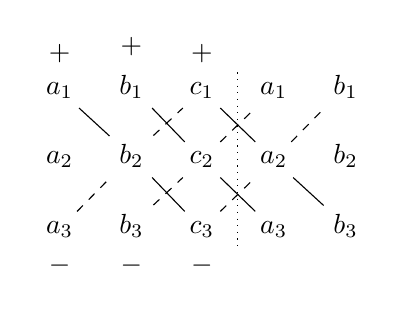
\begin{tikzpicture}
      \matrix [%
        matrix of math nodes,
        column sep=1em,
        row sep=1em
      ] (sarrus) {%
        a_1 & b_1 & c_1 & a_1 & b_1 \\
        a_2 & b_2 & c_2 & a_2 & b_2 \\
        a_3 & b_3 & c_3 & a_3 & b_3 \\
      };

      \path ($(sarrus-1-3.north east)+(0.5em,0)$) edge[dotted] ($(sarrus-3-3.south east)+(0.5em,0)$)
      (sarrus-1-1)                          edge         (sarrus-2-2)
      (sarrus-2-2)                          edge         (sarrus-3-3)
      (sarrus-1-2)                          edge         (sarrus-2-3)
      (sarrus-2-3)                          edge         (sarrus-3-4)
      (sarrus-1-3)                          edge         (sarrus-2-4)
      (sarrus-2-4)                          edge         (sarrus-3-5)
      (sarrus-3-1)                          edge[dashed] (sarrus-2-2)
      (sarrus-2-2)                          edge[dashed] (sarrus-1-3)
      (sarrus-3-2)                          edge[dashed] (sarrus-2-3)
      (sarrus-2-3)                          edge[dashed] (sarrus-1-4)
      (sarrus-3-3)                          edge[dashed] (sarrus-2-4)
      (sarrus-2-4)                          edge[dashed] (sarrus-1-5);

      \foreach \c in {1,2,3} {\node[anchor=south] at (sarrus-1-\c.north) {$+$};};
      \foreach \c in {1,2,3} {\node[anchor=north] at (sarrus-3-\c.south) {$-$};};
    \end{tikzpicture}
  \end{center}

  Note that the Sarrus method is only applicable to 3x3 matrices.

  \subsection{Practice 5}

  Calculate the value of the following determinants.

  \begin{enumerate}
    \item $\vm{
              1 & 5 & 1 \\
              1 & 6 & 3 \\
              9 & 8 & 9
            }$
          \sol{}

          \begin{center}
            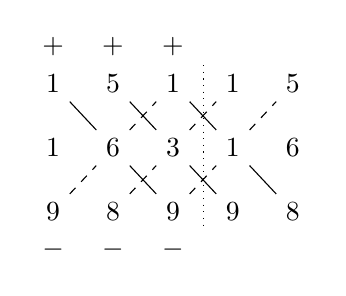
\begin{tikzpicture}
              \matrix [%
                matrix of math nodes,
                column sep=1em,
                row sep=1em
              ] (sarrus) {%
                1 & 5 & 1 & 1 & 5 \\
                1 & 6 & 3 & 1 & 6 \\
                9 & 8 & 9 & 9 & 8 \\
              };

              \path ($(sarrus-1-3.north east)+(0.5em,0)$) edge[dotted] ($(sarrus-3-3.south east)+(0.5em,0)$)
              (sarrus-1-1)                          edge         (sarrus-2-2)
              (sarrus-2-2)                          edge         (sarrus-3-3)
              (sarrus-1-2)                          edge         (sarrus-2-3)
              (sarrus-2-3)                          edge         (sarrus-3-4)
              (sarrus-1-3)                          edge         (sarrus-2-4)
              (sarrus-2-4)                          edge         (sarrus-3-5)
              (sarrus-3-1)                          edge[dashed] (sarrus-2-2)
              (sarrus-2-2)                          edge[dashed] (sarrus-1-3)
              (sarrus-3-2)                          edge[dashed] (sarrus-2-3)
              (sarrus-2-3)                          edge[dashed] (sarrus-1-4)
              (sarrus-3-3)                          edge[dashed] (sarrus-2-4)
              (sarrus-2-4)                          edge[dashed] (sarrus-1-5);

              \foreach \c in {1,2,3} {\node[anchor=south] at (sarrus-1-\c.north) {$+$};};
              \foreach \c in {1,2,3} {\node[anchor=north] at (sarrus-3-\c.south) {$-$};};
            \end{tikzpicture}
          \end{center}
          \begin{flalign*}
            \vm{
            1 & 5                             & 1 \\
            1 & 6                             & 3 \\
            9 & 8                             & 9
            } & = 54 + 135 + 8 - 54 - 24 - 45     \\
              & = 74
          \end{flalign*}
    \item $\vm{
              3 & 1  & -2 \\
              0 & -1 & 1  \\
              4 & 2  & 5
            }$
          \sol{}

          \begin{center}
            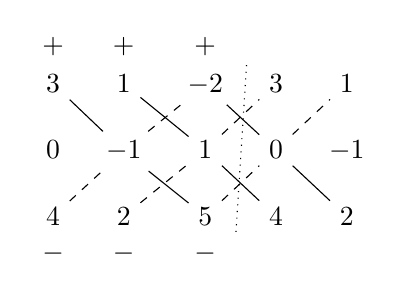
\begin{tikzpicture}
              \matrix [%
                matrix of math nodes,
                column sep=1em,
                row sep=1em
              ] (sarrus) {%
                3 & 1  & -2 & 3 & 1  \\
                0 & -1 & 1  & 0 & -1 \\
                4 & 2  & 5  & 4 & 2  \\
              };

              \path ($(sarrus-1-3.north east)+(0.5em,0)$) edge[dotted] ($(sarrus-3-3.south east)+(0.5em,0)$)
              (sarrus-1-1)                          edge         (sarrus-2-2)
              (sarrus-2-2)                          edge         (sarrus-3-3)
              (sarrus-1-2)                          edge         (sarrus-2-3)
              (sarrus-2-3)                          edge         (sarrus-3-4)
              (sarrus-1-3)                          edge         (sarrus-2-4)
              (sarrus-2-4)                          edge         (sarrus-3-5)
              (sarrus-3-1)                          edge[dashed] (sarrus-2-2)
              (sarrus-2-2)                          edge[dashed] (sarrus-1-3)
              (sarrus-3-2)                          edge[dashed] (sarrus-2-3)
              (sarrus-2-3)                          edge[dashed] (sarrus-1-4)
              (sarrus-3-3)                          edge[dashed] (sarrus-2-4)
              (sarrus-2-4)                          edge[dashed] (sarrus-1-5);

              \foreach \c in {1,2,3} {\node[anchor=south] at (sarrus-1-\c.north) {$+$};};
              \foreach \c in {1,2,3} {\node[anchor=north] at (sarrus-3-\c.south) {$-$};};
            \end{tikzpicture}
          \end{center}
          \begin{flalign*}
            \vm{
            3 & 1                         & -2 \\
            0 & -1                        & 1  \\
            4 & 2                         & 5
            } & = -15 + 4 - 0 - 8 - 6 - 0      \\
              & = -25
          \end{flalign*}
  \end{enumerate}
  \subsection*{Minor and Cofactor}

  The minor of an element in a matrix is the determinant of the matrix obtained
  by deleting the row and column containing the element. Take $\vm{ a_1 & a_2 &
      a_3 \\ b_1 & b_2 & b_3 \\ c_1 & c_2 & c_3 }$ as an example. The minor of $a_1$
  is $\vm{ b_2 & c_2 \\ b_3 & c_3 }$, the minor of $c_2$ is $\vm{ a_1 & b_1 \\
      a_3 & b_3 }$, and so on.

  The cofactor of an element in a matrix is the minor of the element multiplied
  by ${(-1)}^{i+j}$, where $i$ and $j$ are the row and column indices of the
  element. The cofactor of $a_1$ is ${(-1)}^{1+1}\vm{ b_2 & c_2 \\ b_3 & c_3 }$,
  the cofactor of $c_2$ is ${(-1)}^{3+2}\vm{ a_1 & b_1 \\ a_3 & b_3 }$, and so
  on.

  Let $A_1, B_1, C_1$ are the cofactors of $a_1, b_1, c_1$ respectively. Then

  \makeatletter
  \setbool{@fleqn}{false}
  \makeatother
  \begin{flalign*}
    A_1 & = (-1)^{1+1}\vm{ b_2 & c_2 \\ b_3 & c_3 } = \vm{ b_2 & c_2 \\ b_3 & c_3 }  \\
    B_1 & = (-1)^{1+2}\vm{ a_2 & c_2 \\ a_3 & c_3 } = -\vm{ a_2 & c_2 \\ a_3 & c_3 } \\
    C_1 & = (-1)^{1+3}\vm{ a_2 & b_2 \\ a_3 & b_3 } = \vm{ a_2 & b_2 \\ a_3 & b_3 }
  \end{flalign*}
  \makeatletter
  \setbool{@fleqn}{true}
  \makeatother

  Thus,
  \begin{cequation}
    |A| =  a_1A_1 + a_2B_1 + a_3C_1
  \end{cequation}

  That is, the value of the determinant is the elements of the first row
  multiplied by the cofactors of the elements of the first row.

  The sign of the cofactor is determined by the sum of the row and column indices
  of the element. If the sum is even, the cofactor is positive; if the sum is
  odd, the cofactor is negative.\newline\newline \noindent Generally, a 3x3
  determinant has the following theorem:

  \begin{theorem}
    The determinant of a 3x3 matrix is the sum of the elements of any row or
    column multiplied by the cofactors of the elements of that row or column.
  \end{theorem}

  That is, we can use the cofactor expansion to calculate the determinant of a
  3x3 matrix.

  \makeatletter
  \setbool{@fleqn}{false}
  \makeatother
  \begin{flalign*}
    \vm{A} & = a_1A_1 + b_1B_1 + c_1C_1 \\
           & = a_2B_2 + b_2B_2 + c_2C_2 \\
           & = a_3C_3 + b_3C_3 + c_3C_3 \\
           & = a_1A_1 + a_2A_2 + a_3A_3 \\
           & = b_1B_1 + b_2B_2 + b_3B_3 \\
           & = c_1C_1 + c_2C_2 + c_3C_3
  \end{flalign*}
  \makeatletter
  \setbool{@fleqn}{true}
  \makeatother

  The determinant of any order matrix can also be calculated by the cofactor
  expansion.

  \begin{theorem}
    The product of the elements of any row or column and the cofactor of corresponding elements of another row or column of a determinant is 0.
  \end{theorem}
  For example, the product of the elements of the second row and the corresponding element of the cofactor of first row of the determinant is 0. That is,
  \begin{flalign*}
     & a_2B_1 + b_2B_1 + c_2C_1                                                      \\
     & = a_2\vm{ b_2                                                           & c_2 \\ b_3 & c_3 } - b_2\vm{ a_2 & c_2 \\ a_3 & c_3 } + c_2\vm{ a_2 & b_2 \\ a_3 & b_3 } \\
     & = a_2b_2c_3 + a_2b_3c_2 - a_2b_2c_3 + a_3b_2c_2 + a_2b_3c_2 - a_3b_2c_2       \\
     & = 0
  \end{flalign*}

  \subsection{Practice 6}
  Find the value of the following 3x3 determinants.

  \begin{enumerate}
    \item $\vm{ 4 & -2 & 1 \\ 1 & -3 & 0 \\ 2 & 7 & -1 }$
          \sol{}
          \begin{flalign*}
             & \vm{ 4                          & -2 & 1 \\ 1 & -3 & 0 \\ 2 & 7 & -1 }                                                                            \\
             & = 4\vm{ - 3                     & 0      \\ 7 & -1 } - \vm{ -2 & 1 \\ 7 & -1 } + 2 \vm{ -2 & 1 \\ -3 & 0 } \\
             & = 4(3 - 0) - (2 - 7) + 2(0 + 3)          \\
             & = 12 + 5 + 6                             \\
             & = 23
          \end{flalign*}

    \item $\vm{ 5 & -4 & 2 \\ 1 & 0 & -3 \\ 1 & -1 & 2 }$
          \sol{}
          \begin{flalign*}
             & \vm{ 5                           & -4 & 2 \\ 1 & 0 & -3 \\ 1 & -1 & 2 }                                                                         \\
             & = 5\vm{ 0                        & -3     \\ -1 & 2 } - \vm{ -4 & 2 \\ -1 & 2 } + \vm{ -4 & 2 \\ 0 & -3 } \\
             & = 5(0 - 3) - (-8 + 2) + (12 + 0)          \\
             & = -15 + 6 + 12                            \\
             & = 3
          \end{flalign*}

    \item $\vm{ 2 & 0 & 1 \\ 0 & 2 & 0 \\ 2 & 0 & -1 }$
          \sol{}
          \begin{flalign*}
             & \vm{ 2              & 0 & 1 \\ 0 & 2 & 0 \\ 2 & 0 & -1 }                                                                         \\
             & = 2\vm{ 2           & 0     \\ 0 & -1 } - 0\vm{ 0 & 1 \\ 0 & -1 } + 2\vm{ 0 & 1 \\ 2 & 0 } \\
             & = 2(-2 - 0) + 2(-2)         \\
             & = -4 - 4                    \\
             & = -8
          \end{flalign*}
  \end{enumerate}

  \subsection{Exercise 14.5a}

  Find the value of the following determinants.

  \begin{enumerate}
    \item $\vm{ 3 & 2 \\ 1 & -4 }$
          \sol{}
          \begin{flalign*}
             & \vm{ 3         & 2 \\ 1 & -4 } \\
             & = 3(-4) - 2(1)     \\
             & = -12 - 2          \\
             & = -14
          \end{flalign*}

    \item $\vm{ 35 & -2 \\ -11 & 5 }$
          \sol{}
          \begin{flalign*}
             & \vm{ 35             & -2 \\ -11 & 5 } \\
             & = 35(5) - (-2)(-11)      \\
             & = 175 - 22               \\
             & = 153
          \end{flalign*}

    \item $\vm{ 1 & a \\ -a & 1 }$
          \sol{}
          \begin{flalign*}
             & \vm{ 1         & a \\ -a & 1 } \\
             & = 1(1) - a(-a)     \\
             & = 1 + a^2          \\
          \end{flalign*}

    \item $\vm{ \sin{x} & -\cos{x} \\ \cos{x} & \sin{x} }$
          \sol{}
          \begin{flalign*}
             & \vm{ \sin{x}                           & -\cos{x} \\ \cos{x} & \sin{x} } \\
             & = \sin{x}\sin{x} - (-\cos{x})(\cos{x})            \\
             & = \sin^2{x} + \cos^2{x}                           \\
             & = 1
          \end{flalign*}

    \item $\vm{ 1 & -2 & 3 \\ 2 & 3 & -4 \\ 3 & -2 & 5 }$
          \sol{}
          \begin{flalign*}
             & \vm{ 1                              & -2 & 3 \\ 2 & 3 & -4 \\ 3 & -2 & 5 }                                                                           \\
             & = 1\vm{ 3                           & -4     \\ -2 & 5 } - 2\vm{ -2 & 3 \\ -2 & 5 } + 3\vm{ -2 & 3 \\ 3 & -4 } \\
             & = 1(15 - 8) - 2(-10 + 6) + 3(8 - 9)          \\
             & = 7 + 8 - 3                                  \\
             & = 12                                         \\
          \end{flalign*}

    \item $\vm{ 1 & -3 & 4 \\ 2 & 0 & -5 \\ 3 & -1 & 7 }$
          \sol{}
          \begin{flalign*}
             & \vm{ 1                             & -3 & 4 \\ 2 & 0 & -5 \\ 3 & -1 & 7 }                                                                          \\
             & = \vm{ 0                           & -5     \\ -1 & 7 } - 2\vm{ -3 & 4 \\ -1 & 7 } + 3\vm{ -3 & 4 \\ 0 & -5 } \\
             & = (0 - 5) - 2(-21 + 4) + 3(15 - 0)          \\
             & = -5 + 34 + 45                              \\
             & = 74
          \end{flalign*}

    \item $\vm{ -1 & 3 & -2 \\ -3 & 2 & 0 \\ 4 & 0 & 5 }$
          \sol{}
          \begin{flalign*}
             & \vm{ -1                          & 3 & -2 \\ -3 & 2 & 0 \\ 4 & 0 & 5 }                                                                       \\
             & = -1\vm{ 2                       & 0      \\ 0 & 5 } + 3\vm{ 3 & -2 \\ 0 & 5 } + 4\vm{ 3 & -2 \\ 2 & 0 } \\
             & = -1(10) + 3(-15 + 0) + 4(0 + 4)          \\
             & = -10 + 45 + 16                           \\
             & = 51
          \end{flalign*}

    \item $\vm{ 0 & -q & -r \\ q & 0 & -s \\ r & s & 0 }$
          \sol{}
          \begin{flalign*}
             & \vm{ 0                      & -q & -r \\ q & 0 & -s \\ r & s & 0 }                                                                          \\
             & = 0\vm{ 0                   & -s      \\ s & 0 } - q\vm{ -q & -r \\ s & 0 } + r\vm{ -q & -r \\ 0 & -s } \\
             & = 0 - q(0 + sr) + r(0 + qs)           \\
             & = 0
          \end{flalign*}

    \item $\vm{ p & -q & r \\ q & r & -s \\ -r & s & p }$
          \sol{}
          \begin{flalign*}
             & \vm{ p                                    & -q & r \\ q & r & -s \\ -r & s & p }                                                                         \\
             & = p\vm{ r                                 & -s     \\ s & p } - q\vm{ -q & r \\ s & p } + r\vm{ -q & r \\ r & -s } \\
             & = p(rp + s^2) -q(-qp - sr) - r(qs - r^2)           \\
             & = rp^2 + p{s}^2 + q^2 p + qsr - qsr + r^3          \\
             & = rp^2 + s^2p + q^2 p - r^3
          \end{flalign*}

    \item $\vm{ 1 & x & a \\ 1 & y & b \\ 1 & z & c }$
          \sol{}
          \begin{flalign*}
             & \vm{ 1                              & x & a \\ 1 & y & b \\ 1 & z & c }                                                                    \\
             & = \vm{ y                            & b     \\ z & c } - \vm{ x & a \\ z & c } + \vm{ x & a \\ y & b } \\
             & = (yc - bz) - (xc - az) + (xb - ay)         \\
             & = bx + cy + az - cx - ay - bz               \\
          \end{flalign*}
  \end{enumerate}

  \subsection*{Identities of Determinants}

  \setcounter{theorem}{0}

  \begin{theorem}
    The value of a determinant is the same as the value of its transpose, aka $|A| = |A'|$.
    \begin{cequation}
      \vm{ a & b \\ c & d } = \vm{ a & c \\ b & d }
    \end{cequation}
  \end{theorem}
  \begin{theorem}
    Switching any two rows or columns of a determinants results in the opposite value.
    \begin{cequation}
      \vm{ a_1 & b_1 & c_1 \\ a_2 & b_2 & c_2 \\ a_3 & b_3 & c_3 } = -\vm{ a_1 & b_1 & c_1 \\ a_3 & b_3 & c_3 \\ a_2 & b_2 & c_2 }
    \end{cequation}
  \end{theorem}

  \subsection{Practice 7}

  Given $\vm{ a & b & c \\ d & e & f \\ g & h & i } = 10$, find $\vm{ b & c & a
      \\ e & f & d \\ h & i & g }$. \sol{}
  \begin{flalign*}
    \vm{
    b & c       & a \\
    e & f       & d \\
    h & i       & g
    }
      & = -\vm{
    a & c       & b \\
    d & f       & e \\
    g & i       & h
    }               \\
      & = \vm{
    a & b       & c \\
    d & e       & f \\
    g & h       & i
    }               \\
      & = 10
  \end{flalign*}
  \begin{theorem}
    If two rows or cols of a determinant are identical, the value of the determinant is zero.
    \begin{cequation}
      \vm{ a & b & c \\ a & b & c \\ d & e & f } = 0 \\
    \end{cequation}
  \end{theorem}
  \begin{theorem}
    If all elements of a row (or column) of a determinant are multiplied by some scalar number k, the value of the new determinant is k times of the given determinant.
    \begin{cequation}
      \vm{ a_1 & b_1 & c_1 \\ ka_2 & kb_2 & kc_2 \\ a_3 & b_3 & c_3 } = k\vm{ a_1 & b_1 & c_1 \\ a_2 & b_2 & c_2 \\ a_3 & b_3 & c_3 }
    \end{cequation}
  \end{theorem}

  \subsection{Practice 8}

  Using the identities of determinants, prove that $\vm{ 10 & -12 & 2 \\ -15 & 18
      & 3 \\ 5 & 6 & -1 } = 180\vm{ 1 & -1 & 1 \\ -1 & 1 & 1 \\ 1 & 1 & -1 }$. \sol{}
  \begin{flalign*}
       & \vm{ 10                        & -12 & 2 \\ -15 & 18 & 3 \\ 5 & 6 & -1 } \\
       & = 5\cdot6\vm{
    2  & -2                             & 2       \\
    -3 & 3                              & 3       \\
    1  & 1                              & -1
    }                                             \\
       & = 5\cdot6\cdot2\cdot3\cdot\vm{
    1  & -1                             & 1       \\
    -1 & 1                              & 1       \\
    1  & 1                              & -1
    }                                             \\
       & = 180\vm{
    1  & -1                             & 1       \\
    -1 & 1                              & 1       \\
    1  & 1                              & -1
    }
  \end{flalign*}

  \begin{theorem}
    In a determinant each element in any row (or column) consists of the sum of two terms, then the determinant can be expressed as sum of two determinants of same order.
    \begin{cequation}
      \vm{ a_1+d_1 & b_1 & c_1 \\ a_2+d_2 & b_2 & c_2 \\ a_3+d_3 & b_3 & c_3 } = \vm{ a_1 & b_1 & c_1 \\ a_2 & b_2 & c_2 \\ a_3 & b_3 & c_3 } + \vm{ d_1 & b_1 & c_1 \\ d_2 & b_2 & c_2 \\ d_3 & b_3 & c_3 }
    \end{cequation}
  \end{theorem}
  \begin{theorem}
    If a determinant is obtained by adding a row or column multiplied by a some scalar number k to a different row or column, then the value of the new determinant is the same as the original determinant.
    \begin{cequation}
      \vm{ a_1 & b_1 & c_1 \\ a_2 & b_2 & c_2 \\ a_3 & b_3 & c_3 } = \vm{ a_1+ka_2 & b_1+kb_2 & c_1+kc_2 \\ a_2 & b_2 & c_2 \\ a_3 & b_3 & c_3 }
    \end{cequation}
  \end{theorem}

  \subsection{Practice 9}

  Prove that $\vm{ 1 & 2 & 3 \\ 4 & 5 & 6 \\ 7 & 8 & 9 } = 0$. \sol{}
  \begin{flalign*}
     & \vm{ 1    & 2                  & 3 \\ 4 & 5 & 6 \\ 7 & 8 & 9 }                                                            \\
     & = \vm{ 1  & 2                  & 3 \\ 3 & 3 & 3 \\ 6 & 6 & 6 }  & (\text{Adding row 1 multiplied by -1 to row 2 and 3}) \\
     & = 2\vm{ 1 & 2                  & 3 \\ 3 & 3 & 3 \\ 3 & 3 & 3 } & (\text{Theorem 4})                                    \\
     & = 0       & (\text{Theorem 3})
  \end{flalign*}

  \begin{theorem}
    The determinant of product of two matrices of equal size is equal to the product of determinants of each matrix, aka $|AB| = |A||B|$.
  \end{theorem}

  \subsection{Practice 10}

  Let $A = \vm{ -2 & 1 \\ 4 & 3 }$ and $B = \vm{ 1 & x \\ 2 & 3 }$. Given that
  $|AB| = -18$, find $x$. \sol{}
  \begin{flalign*}
    \because\ |AB| = |A||B| & = -18 \\
    \therefore\ \vm{
    -2                      & 1     \\
    4                       & 3
    }\vm{
    1                       & x     \\
    2                       & 3
    }                       & = -18 \\
    -2(3-2x)                & = -18 \\
    3-2x                    & = 9   \\
    -2x                     & = 6   \\
    x                       & = -3
  \end{flalign*}

  \subsection{Exercise 14.5b}

  \begin{enumerate}

    \item Given $\vm{ 2 & -2 & 3 \\ 0 & -1 & -2 \\ -1 & 2 & 1 } = -1$, Find the value of
          the following determinants.

          \begin{enumerate}
            \item $\vm{
                      2  & 0  & -1 \\
                      -2 & -1 & 2  \\
                      3  & -2 & 1
                    }$
                  \sol{}
                  \begin{flalign*}
                       & \vm{
                    2  & 0          & -1                 \\
                    -2 & -1         & 2                  \\
                    3  & -2         & 1
                    }                                    \\
                       & =\left|\m{
                    2  & -2         & 3                  \\
                    0  & -1         & -2                 \\
                    -1 & 2          & 1
                    }' \right|                           \\
                       & =-1        & (\text{Theorem 1}) \\
                  \end{flalign*}
            \item $\vm{
                      2  & 0  & -1 \\
                      3  & -2 & 1  \\
                      -2 & -1 & 2
                    }$
                  \sol{}
                  \begin{flalign*}
                       & \vm{
                    2  & 0    & -1 \\
                    3  & -2   & 1  \\
                    -2 & -1   & 2
                    }              \\
                  \end{flalign*}
                  \sol{}
                  \begin{flalign*}
                       & \vm{
                    2  & 0           & -1                 \\
                    3  & -2          & 1                  \\
                    -2 & -1          & 2
                    }                                     \\
                       & = -\vm{
                    2  & 0           & -1                 \\
                    -2 & -1          & 2                  \\
                    3  & -2          & 1
                    }                                     \\
                       & =-\left|\m{
                    2  & -2          & 3                  \\
                    0  & -1          & -2                 \\
                    -1 & 2           & 1
                    }' \right|                            \\
                       & =1          & (\text{Theorem 1}) \\
                  \end{flalign*}
            \item $\vm{
                      4  & -2 & 3  \\
                      0  & -2 & -4 \\
                      -2 & 2  & 1
                    }$
                  \sol{}
                  \begin{flalign*}
                       & \vm{
                    4  & -2            & 3  \\
                    0  & -2            & -4 \\
                    -2 & 2             & 1
                    }  &                    \\
                       & = 2\cdot2\vm{
                    2  & -2            & 3  \\
                    0  & -1            & -2 \\
                    -1 & 2             & 1
                    }  &                    \\
                       & = -4
                  \end{flalign*}
            \item $\vm{
                      -3 & -2 & -2 \\
                      2  & -1 & 0  \\
                      -1 & 2  & 1
                    }$
                  \sol{}
                  \begin{flalign*}
                       & \vm{
                    -3 & -2     & -2 \\
                    2  & -1     & 0  \\
                    -1 & 2      & 1
                    }  &             \\
                       & = \vm{
                    3  & -2     & 2  \\
                    -2 & -1     & 0  \\
                    1  & 2      & -1
                    }  &             \\
                       & = \vm{
                    2  & -2     & 3  \\
                    0  & -1     & -2 \\
                    -1 & 2      & 1
                    }  &             \\
                       & = 1
                  \end{flalign*}
            \item $\vm{
                      0  & 2  & 5  \\
                      0  & -1 & -2 \\
                      -1 & 2  & 1
                    }$
                  \sol{}
                  \begin{flalign*}
                                   & \vm{
                    0              & 2             & 5             \\
                    0              & -1            & -2            \\
                    - 1            & 2             & 1
                    }                                              \\
                                   & = \vm{
                    2+(2\cdot(-1)) & -2+(-2\cdot2) & 3+(2\cdot1) & \\
                    0              & -1            & -2          & \\
                    -1             & 2             & 1
                    }              &                               \\
                                   & = -1
                  \end{flalign*}
            \item $\vm{
                      2  & 4  & 3  \\
                      0  & -5 & -2 \\
                      -1 & 4  & 1
                    }$
                  \sol{}
                  \begin{flalign*}
                       & \vm{
                    2  & 4               & 3    \\
                    0  & -5              & -2   \\
                    -1 & 4               & 1
                    }                           \\
                       & = \vm{
                    2  & -2+(2\cdot3)    & 3  & \\
                    0  & -1+(2\cdot(-2)) & -2 & \\
                    -1 & 2+(2\cdot1)     & 1
                    }  &                        \\
                       & = -1
                  \end{flalign*}
          \end{enumerate}

    \item Prove the following equations using identities of determinants without
          expanding them.

          \begin{enumerate}
            \item $\vm{
                      1 & 0 & 3  \\
                      4 & 6 & 12 \\
                      3 & 3 & 9  \\
                    } = 0$
                  \prooff{}
                  \begin{flalign*}
                    L.H.S. = & \vm{
                    1        & 0                   & 3                  \\
                    4        & 6                   & 12                 \\
                    3        & 3                   & 9                  \\
                    }                                                   \\
                             & = 2\cdot3\vm{
                    1        & 0                   & 3                  \\
                    2        & 3                   & 6                  \\
                    1        & 1                   & 3                  \\
                    }                                                   \\
                             & = 2\cdot3\cdot3\vm{
                    1        & 0                   & 1                  \\
                    2        & 3                   & 2                  \\
                    1        & 1                   & 1                  \\
                    }                                                   \\
                             & = 0 = R.H.S.        & (\text{Theorem 3})
                  \end{flalign*}

            \item $\vm{
                      2  & -1 & 3 \\
                      -1 & 1  & 2 \\
                      4  & -2 & 6
                    } = 0$
                  \prooff{}
                  \begin{flalign*}
                    L.H.S. & = \vm{
                    2      & -1            & 3                  \\
                    -1     & 1             & 2                  \\
                    4      & -2            & 6
                    }                                           \\
                           & = 2\vm{
                    2      & -1            & 3                  \\
                    -1     & 1             & 2                  \\
                    2      & -1            & 3
                    }                                           \\
                           & = 0  = R.H.S. & (\text{Theorem 3})
                  \end{flalign*}

            \item $\vm{
                      3  & 2 & 2 \\
                      9  & 6 & 5 \\
                      12 & 8 & 8
                    } = 0$
                  \prooff{}
                  \begin{flalign*}
                    L.H.S. & = \vm{
                    3      & 2            & 2                  \\
                    9      & 6            & 5                  \\
                    12     & 8            & 8
                    }      &                                   \\
                           & = 4\vm{
                    3      & 2            & 2                  \\
                    9      & 6            & 5                  \\
                    3      & 2            & 2
                    }      &                                   \\
                           & = 0 = R.H.S. & (\text{Theorem 3})
                  \end{flalign*}
            \item $\vm{
                      10 & 8  & 2  \\
                      15 & 12 & 3  \\
                      20 & 32 & 12
                    } = 0$
                  \prooff{}
                  \begin{flalign*}
                    L.H.S. & = \vm{
                    10     & 8                               & 2                  \\
                    15     & 12                              & 3                  \\
                    20     & 32                              & 12
                    }      &                                                      \\
                           & = 2\cdot3\cdot4\vm{
                    5      & 4                               & 1                  \\
                    5      & 4                               & 1                  \\
                    5      & 8                               & 3
                    }      &                                                      \\
                           & = 2\cdot3\cdot4\cdot5\cdot4\vm{
                    1      & 1                               & 1                  \\
                    1      & 1                               & 1                  \\
                    1      & 2                               & 3
                    }      &                                                      \\
                           & = 0 = R.H.S.                    & (\text{Theorem 3})
                  \end{flalign*}
            \item $\vm{
                      1 & -4 & 5  \\
                      2 & 3  & -2 \\
                      7 & 3  & 0
                    } = \vm{
                      -4 & 3  & 3 \\
                      5  & -2 & 0 \\
                      1  & 2  & 7
                    }$
                  \prooff{}
                  \begin{flalign*}
                    L.H.S     & = \vm{
                    1         & -4                 & 5  \\
                    2         & 3                  & -2 \\
                    7         & 3                  & 0
                    }         &                         \\
                              & = -\vm{
                    5         & -4                 & 1  \\
                    -2        & 3                  & 2  \\
                    0         & 3                  & 7
                    }         &                         \\
                              & = \vm{
                    -4        & 5                  & 1  \\
                    3         & -2                 & 2  \\
                    3         & 0                  & 7
                    }         & (\text{Theorem 2})      \\
                              & = \left|\m{
                    -4        & 5                  & 1  \\
                    3         & -2                 & 2  \\
                    3         & 0                  & 7
                    }'\right| & (\text{Theorem 1})      \\
                              & = \vm{
                    -4        & 3                  & 3  \\
                    5         & -2                 & 0  \\
                    1         & 2                  & 7
                    } = R.H.S.
                  \end{flalign*}
            \item $\vm{
                      -6 & 6  & 3  \\
                      0  & -9 & -3 \\
                      3  & -3 & -6
                    } = -27\vm{
                      1  & -1 & 2  \\
                      3  & 0  & 1  \\
                      -2 & 2  & -1 \\
                    }$
                  \prooff{}
                  \begin{flalign*}
                               & L.H.S.              &    \\
                               & = \vm{
                    -6         & 6                   & 3  \\
                    0          & -9                  & -3 \\
                    3          & -3                  & -6
                    }          &                          \\
                               & = 3\cdot3\cdot3\vm{
                    -2         & 2                   & 1  \\
                    0          & -3                  & -1 \\
                    1          & -1                  & -2 \\
                    }          &                          \\
                               & = -27\vm{
                    1          & -1                  & -2 \\
                    0          & -3                  & -1 \\
                    -2         & 2                   & 1
                    }          & (\text{Theorem 2})       \\
                               & = 27\vm{
                    -1         & 1                   & -2 \\
                    -3         & 0                   & -1 \\
                    2          & -2                  & 1
                    }          & (\text{Theorem 2})       \\
                               & = -27\vm{
                    1          & -1                  & 2  \\
                    3          & 0                   & 1  \\
                    -2         & 2                   & -1 \\
                    } = R.H.S. & (\text{Theorem 4})
                  \end{flalign*}
            \item $\vm{
                      1 & 0  & -3 \\
                      3 & -2 & 4  \\
                      1 & 3  & -2
                    } = \vm{
                      1  & 0 & -3 \\
                      -1 & 2 & 4  \\
                      7  & 3 & -2
                    }$
                  \prooff{}
                  \begin{flalign*}
                                     & L.H.S.             &    \\
                                     & = \vm{
                    1                & 0                  & -3 \\
                    3                & -2                 & 4  \\
                    1                & 3                  & -2
                    }                &                         \\
                                     & = \vm{
                    1 + (2\cdot 0)   & 0                  & -3 \\
                    3 + (2\cdot(-2)) & -2                 & 4  \\
                    1 + (2\cdot 3)   & 3                  & -2
                    }                & (\text{Theorem 6})      \\
                                     & = \vm{
                    1                & 0                  & -3 \\
                    -1               & 2                  & 4  \\
                    7                & 3                  & -2
                    }  = R.H.S.
                  \end{flalign*}
            \item $\vm{
                      5 & 1  & -1 \\
                      2 & -1 & -1 \\
                      1 & -2 & 4
                    } = \vm{
                      3 & 1  & 0  \\
                      4 & -1 & -2 \\
                      5 & -2 & 2
                    }$
                  \prooff{}
                  \begin{flalign*}
                                      & L.H.S.             &      \\
                                      & = \vm{
                    5                 & 1                  & -1   \\
                    2                 & -1                 & -1   \\
                    1                 & -2                 & 4
                    }                 &                           \\
                                      & = \vm{
                    5 + (-2\cdot 1)   & 1                  & -1+1 \\
                    2 + (-2\cdot(-1)) & -1                 & -2-1 \\
                    1 + (-2\cdot(-2)) & -2                 & 4-2
                    }
                                      & (\text{Theorem 6})        \\
                                      & = \vm{
                    3                 & 1                  & 0    \\
                    4                 & -1                 & -2   \\
                    5                 & -2                 & 2
                    } = R.H.S.
                  \end{flalign*}
          \end{enumerate}
    \item Let $A = \m{ 7 & -4 \\ -3 & 2 }$ and $B = \m{ 2x+1 & -2 \\ x & 1 }$. Given that
          $|AB| = -22$, find the value of x. \sol{}
          \begin{flalign*}
            \because\ |AB|                = |A||B| & = -22 & \\
            \therefore\ \vm{
            7                                      & -4      \\
            -3                                     & 2
            }\vm{
            2x+1                                   & -2      \\
            x                                      & 1
            }                                      & = -22 & \\
            2(2x+1 + 2x)                           & = -22 & \\
            4x + 1                                 & = -11 & \\
            4x                                     & = -12 & \\
            x                                      & = -3  & \\
          \end{flalign*}
    \item Let $P = \m{ 3a & 3b & 3c \\ d & e & f \\ g & h & i }$ and $Q = \m{ a & d & g
              \\ b & e & h \\ c & f & i }$. Given that $PQ = \m{ 30 & -18 & -33 \\ -6 & 4 & 6
              \\ -11 & 6 & 14 }$, find the value of $|Q|$. \sol{}
          \begin{flalign*}
            \because\ |P||Q| & = |PQ|      &     \\
            \therefore\ \vm{
            3a               & 3b          & 3c  \\
            d                & e           & f   \\
            g                & h           & i
            }\vm{
            a                & d           & g   \\
            b                & e           & h   \\
            c                & f           & i
            }                & = \vm{
            30               & -18         & -33 \\
            -6               & 4           & 6   \\
            -11              & 6           & 14
            }                &                   \\
            3\vm{
            a                & b           & c   \\
            d                & e           & f   \\
            g                & h           & i
            }\vm{
            a                & b           & c   \\
            d                & e           & f   \\
            g                & h           & i
            }                & = \vm{
            30               & -18         & -33 \\
            -6               & 4           & 6   \\
            -11              & 6           & 14
            }                &                   \\
            3{\left(\vm{
            a                & b           & c   \\
            d                & e           & f   \\
            g                & h           & i
            }\right)}^2      & = 3\vm{
            10               & -6          & -11 \\
            -6               & 4           & 6   \\
            -11              & 6           & 14
            }                &                   \\
            {\left(\vm{
            a                & b           & c   \\
            d                & e           & f   \\
            g                & h           & i
            }\right)}^2      & = \vm{
            10               & -6          & -11 \\
            -6               & 4           & 6   \\
            -11              & 6           & 14
            }                &                   \\
                             & =4          &     \\
            \therefore\ |Q|  & = \vm{
            a                & d           & g   \\
            b                & e           & h   \\
            c                & f           & i
            }                &                   \\
                             & = \left|\m{
            a                & b           & c   \\
            d                & e           & f   \\
            g                & h           & i
            }'\right|        &                   \\
                             & =\vm{
            a                & b           & c   \\
            d                & e           & f   \\
            g                & h           & i
            }                &                   \\
                             & = \pm{2}    &     \\
          \end{flalign*}
          Find the value of x in the following equations.
    \item $\vm{
              x   & x  \\
              -2x & -1
            } = 6$
          \sol{}
          \begin{flalign*}
            \vm{
            x                   & x                \\
            -2x                 & -1
            }                   & = 6            & \\
            x\vm{
            1                   & 1                \\
            -2x                 & -1
            }                   & = 6            & \\
            x(-1+2x)            & = 6            & \\
            -x + 2x^2           & = 6            & \\
            2x^2 - x - 6        & = 0            & \\
            (x-2)(2x+3)         & = 0            & \\
            x = 2 \text{ or } x & = -\frac{3}{2} & \\
          \end{flalign*}
    \item $\vm{
              2 & 4 & 0 \\
              2 & 5 & 6 \\
              3 & x & 9
            } = 0$
          \sol{}
          \begin{flalign*}
            \vm{
            2                 & 4              & 0 \\
            2                 & 5              & 6 \\
            3                 & x              & 9
            }                 & = 0            &   \\
            2\cdot3\vm{
            1                 & 2              & 0 \\
            2                 & 5              & 2 \\
            3                 & x              & 3
            }                 & =0             &   \\
            \vm{
            1                 & 2              & 0 \\
            2                 & 5              & 2 \\
            3                 & x              & 3
            }                 & =0             &   \\
            \vm{
            5                 & 2                  \\
            x                 & 3
            } - 2\vm{
            2                 & 0                  \\
            x                 & 3
            }
            + 3\vm{
            2                 & 0                  \\
            5                 & 2
            }                 & =0             &   \\
            15 - 2x - 12 + 12 & =0             &   \\
            -2x               & = -15          &   \\
            x                 & = \frac{15}{2} &   \\
          \end{flalign*}
    \item $\vm{
              1 & 1 & x \\
              1 & x & 1 \\
              x & 1 & 1
            } = 0$
          \sol{}
          \begin{flalign*}
            \vm{
            1                       & 1   & x \\
            1                       & x   & 1 \\
            x                       & 1   & 1
            }                       & = 0 &   \\
            \vm{
            x                       & 1       \\
            1                       & 1
            } - \vm{
            1                       & x       \\
            1                       & 1
            }
            + x\vm{
            1                       & x       \\
            x                       & 1
            }                       & = 0 &   \\
            x - 1 - 1 + x + x - x^3 & = 0 &   \\
            -x^3 + 3x - 2           & = 0 &   \\
            x^3 - 3x + 2            & = 0 &   \\
            (x+2)(x^2-2x+1)         & = 0 &   \\
            x = -2 \text{ or } x    & = 1 &   \\
          \end{flalign*}
    \item $\vm{
              2x-7 & 6 & 9 \\
              3x-5 & 5 & 4 \\
              x-3  & 0 & 1
            } = 0$
          \sol{}
          \begin{flalign*}
            \vm{
            2x-7             & 6     & 9 \\
            3x-5             & 5     & 4 \\
            x-3              & 0     & 1
            }                & = 0   &   \\
            \vm{
            2x               & 6     & 9 \\
            3x               & 5     & 4 \\
            x                & 0     & 1
            } + \vm{
            -7               & 6     & 9 \\
            -5               & 5     & 4 \\
            -3               & 0     & 1
            }                & = 0   &   \\
            \vm{
            2x               & 6     & 9 \\
            3x               & 5     & 4 \\
            x                & 0     & 1
            }                & = -58 &   \\
            x\vm{
            6                & 9         \\
            5                & 4
            } + \vm{
            2x               & 6         \\
            3x               & 5
            }                & = -58 &   \\
            -21x + 10x - 18x & = -58 &   \\
            -29x             & = -58 &   \\
            x                & = 2   &   \\
          \end{flalign*}
    \item $\vm{
              15-2x & 11 & 10 \\
              11-3x & 17 & 16 \\
              7-x   & 14 & 13
            } = 0$
          \sol{}
          \begin{flalign*}
            \vm{
            15-2x         & 11    & 10 \\
            11-3x         & 17    & 16 \\
            7-x           & 14    & 13
            }             & = 0   &    \\
            \vm{
            15            & 11    & 10 \\
            11            & 17    & 16 \\
            7             & 14    & 13
            } + \vm{
            -2x           & 11    & 10 \\
            -3x           & 17    & 16 \\
            -x            & 14    & 13
            }             & = 0   &    \\
            \vm{
            -2x           & 11    & 10 \\
            -3x           & 17    & 16 \\
            -x            & 14    & 13
            } = 36        &            \\
            -2x \vm{
            17            & 16         \\
            14            & 13
            } + 3x\vm{
            11            & 10         \\
            14            & 13
            } - x\vm{
            11            & 10         \\
            17            & 16
            }             & = 36  &    \\
            x\left(2 \vm{
            17            & 16         \\
            14            & 13
            } - 3\vm{
            11            & 10         \\
            14            & 13
            } + \vm{
            11            & 10         \\
            17            & 16
            }\right)      & = -36 &    \\
            (-6 - 9 + 6)x & = -36 &    \\
            -9x           & = -36 &    \\
            x             & = 4   &    \\
          \end{flalign*}
    \item $\vm{
              x-1 & 0   & x-3 \\
              1   & x-2 & 1   \\
              2   & x-2 & 2
            } = 0$
          \sol{}
          \begin{flalign*}
            \vm{
            x-1                                        & 0   & x-3 \\
            1                                          & x-2 & 1   \\
            2                                          & x-2 & 2
            }                                          & = 0 &     \\
            (x-2)\vm{
            x-1                                        & 0   & x-3 \\
            1                                          & 1   & 1   \\
            2                                          & 1   & 2
            }                                          & = 0 &     \\
            (x-2)\left(
            -\vm{
            x-1                                        & x-3       \\
            2                                          & 2
            }
            + \vm{
            x-1                                        & x-3       \\
            1                                          & 1
            }
            \right)                                    & = 0 &     \\
            (x-2)\left[-(2x-2-2x+6) + (x-1-x-3)\right] & = 0 &     \\
            (x-2)                                      & = 0 &     \\
            x                                          & = 2 &     \\
          \end{flalign*}
  \end{enumerate}

  \section{Inverse Matrix}

  If two square matrices $A$ and $B$ are of the same order such that $AB=BA=I$,
  while $I$ is an identity matrix that has the same order as $A$ and $B$, then
  $A$ and $B$ are said to be inverse matrices of each other, and can be denoted
  as $B = A^{-1}$ and $A = B^{-1}$.

  Note that only square matrix have inverse matrix. If a matrix has an inverse
  matrix, then it is said to be invertible, and the inverse matrix is unique.

  \subsection*{Inverse Matrix of a 2x2 Matrix}

  Let $A = \m{ a & b \\ c & d }$ be a 2x2 matrix. Then
  \begin{cequation}
    A^{-1} = \frac{1}{ad-bc} \m{ d & -b \\ -c & a }
    \ \ \ \ \ (ad-bc \neq 0)
  \end{cequation}

  If $|A| = ad - bc = 0$, then $A$ is said to be non-invertible.

  \subsection{Practice 11}

  Determine if the following matrices are invertible. If they are, find their
  inverse matrices.

  \begin{enumerate}
    \item $\m{ 6 & 3 \\ 7 & 5 }$
          \sol{}
          \begin{flalign*}
            |A|           & = 6 \cdot 5 - 3 \cdot 7 = 9 \neq 0                \\
            \therefore\ A & \text{ is invertible.}                            \\
            A^{-1}        & = \frac{1}{9} \m{ 5                & -3           \\ -7 & 6 }                             \\
                          & = \m{ \frac{5}{9}                  & -\frac{1}{1} \\ -\frac{7}{9} & \frac{2}{3} }
          \end{flalign*}
    \item $\m{
              -3 & -2 \\
              6  & 4
            }$
          \sol{}
          \begin{flalign*}
            |A|           & = -3 \cdot 4 - (-2) \cdot 6 = 0 \\
            \therefore\ A & \text{ is non-invertible.}
          \end{flalign*}
    \item $\m{ 2 & -6 \\ 3 & -5 }$
          \sol{}
          \begin{flalign*}
            |A|           & = 2 \cdot -5 - (-6) \cdot 3 = 8 \neq 0               \\
            \therefore\ A & \text{ is invertible.}                               \\
            A^{-1}        & = \frac{1}{8} \m{ -5                   & 6           \\ -3 & 2 }                             \\
                          & = \m{ -\frac{5}{8}                     & \frac{3}{4} \\ -\frac{3}{8} & \frac{1}{4} }
          \end{flalign*}

    \item If $\m{ 2b+1 & 2 \\ -3b-3 & -4 }$ is non-invertible, find the value of $b$.
          \sol{}
          \begin{flalign*}
            \because\ \text{The matrix is no} & \text{n-invertible} \\
            \therefore\ \vm{
            2b+1                              & 2                   \\
            -3b-3                             & -4
            }                                 & = 0                 \\
            -8b -4 + 6b + 6                   & = 0                 \\
            -2b + 2                           & = 0                 \\
            b                                 & = 1
          \end{flalign*}
  \end{enumerate}
  \subsection*{Inverse Matrix of a 3x3 Matrix}

  Let a 3x3 matrix $A$ be of the form $A = \m{ a_1 & b_1 & c_1 \\ a_2 & b_2 & c_2
      \\ a_3 & b_3 & c_3 }$. Arrange all the cofactors of elements in $A$ into a
  matrix:
  \begin{cequation}
    \m{
      A_1 & B_1 & C_1 \\
      A_2 & B_2 & C_2 \\
      A_3 & B_3 & C_3
    }
  \end{cequation}

  Then the transpose of the matrix is the adjoint matrix of $A$, and can be
  denoted as $\operatorname{adj}A$. That is:
  \begin{cequation}
    \operatorname{adj}A = \m{
      A_1 & A_2 & A_3 \\
      B_1 & B_2 & B_3 \\
      C_1 & C_2 & C_3
    }
  \end{cequation}
  The inverse matrix of $A$ is:
  \begin{cequation}
    A^{-1} = \frac{1}{|A|} \operatorname{adj}A
    \ \ \ \ \ (|A| \neq 0)
  \end{cequation}

  \subsection{Practice 12}

  Find the inverse matrix of the following matrices.

  \begin{enumerate}
    \item $\m{
              -1 & 2  & 3  \\
              3  & 0  & 1  \\
              2  & -1 & -2
            }$
          \sol{}
          \begin{flalign*}
                                        & |A| = \vm{
            -1                          & 2                & 3           \\
            3                           & 0                & 1           \\
            2                           & -1               & -2          \\
            } = 6                       &                                \\
                                        & \m{
            \vm{ 0                      & 1                              \\ -1 & -2 }  & -\vm{ 3 & 1 \\ 2 & -2 } & \vm{ 3 & 0 \\ 2 & -1 }   \\
            -\vm{ 2                     & 3                              \\ -1 & -2 } & \vm{ -1 & 3 \\ 2 & -2 } & -\vm{ -1 & 2 \\ 2 & -1 } \\
            \vm{ 2                      & 3                              \\ 0 & 1 }    & -\vm{ -1 & 3 \\ 3 & 1 } & \vm{ -1 & 2 \\ 3 & 0 }
            }                                                            \\
                                        & =\m{
            1                           & 8                & -3          \\
            1                           & -4               & 3           \\
            2                           & 10               & -6
            }                           &                                \\
            \operatorname{adj}A         & = \m{
            1                           & 1                & 2           \\
            8                           & -4               & 10          \\
            -3                          & 3                & -6
            }                           &                                \\
            \therefore\          A^{-1} & = \frac{1}{6}\m{
            1                           & 1                & 2           \\
            8                           & -4               & 10          \\
            -3                          & 3                & -6
            } = \m{
            \frac{1}{6}                 & \frac{1}{6}      & \frac{1}{3} \\
            \frac{4}{3}                 & -\frac{2}{3}     & \frac{5}{3} \\
            -\frac{1}{2}                & \frac{1}{2}      & -1
            }
          \end{flalign*}
    \item $\m{
              1  & -2 & -1 \\
              -1 & 2  & -3 \\
              1  & 0  & 1
            }$
          \sol{}
          \begin{flalign*}
                                        & |A| = \vm{
            1                           & -2               & -1          \\
            -1                          & 2                & -3          \\
            1                           & 0                & 1
            } = 8                       &                                \\
                                        & \m{
            \vm{ 2                      & -3                             \\ 0 & 1 }   & -\vm{ -1 & -3 \\ 1 & 1 }  & \vm{ -1 & 2 \\ 1 & 0 }  \\
            -\vm{ -2                    & -1                             \\ 0 & 1 } & \vm{ 1 & -1 \\ 1 & 1 }    & -\vm{ 1 & -2 \\ 1 & 0 } \\
            \vm{ -2                     & -1                             \\ 2 & -3 } & -\vm{ 1 & -1 \\ -1 & -3 } & \vm{ 1 & -2 \\ -1 & 2 }
            }                           &                                \\
                                        & = \m{
            2                           & -2               & -2          \\
            2                           & 2                & -2          \\
            8                           & 4                & 0
            }                           &                                \\
            \operatorname{adj}A         & = \m{
            2                           & 2                & 8           \\
            -2                          & 2                & 4           \\
            -2                          & -2               & 0
            }                           &                                \\
            \therefore\          A^{-1} & = \frac{1}{8}\m{
            2                           & 2                & 8           \\
            -2                          & 2                & 4           \\
            -2                          & -2               & 0
            } = \m{
            \frac{1}{4}                 & \frac{1}{4}      & 1           \\
            -\frac{1}{4}                & \frac{1}{4}      & \frac{1}{2} \\
            -\frac{1}{4}                & -\frac{1}{4}     & 0
            }
          \end{flalign*}
  \end{enumerate}

  \subsection*{Solving Systems of Linear Equations}

  Binary and ternary systems of linear equations can be solved by using the
  inverse matrix of the coefficient matrix. Note that the coefficient matrix must
  be invertible for this method to work.

  \subsection{Practice 13}

  Solve the following systems of linear equations using the inverse matrix
  method.

  \begin{enumerate}
    \item $\begin{cases}
              3x - 2y = 12 \\
              7x + 5y = -1
            \end{cases}$
          \sol{}
          \begin{flalign*}
            \text{Let } A & = \m{
            3             & -2                \\
            7             & 5
            }                                 \\
            A\m{
            x                                 \\
            y
            }             & = \m{
            12                                \\
            -1
            }                                 \\
            A^{-1}A\m{
            x                                 \\
            y
            }             & = A^{-1}\m{
            12                                \\
            -1
            }                                 \\
            \m{
            x                                 \\
            y
            }             & = A^{-1}\m{
            12                                \\
            -1
            }                                 \\
                          & = \frac{1}{29}\m{
            5             & 2                 \\
            -7            & 3
            }\m{
            12                                \\
            -1
            }                                 \\
                          & = \frac{1}{29}\m{
            58                                \\
            -87
            }                                 \\
                          & = \m{
            2                                 \\
            -3
            }                                 \\
            \therefore\ x & = 2,\ y = -3
          \end{flalign*}
    \item $\begin{cases}
              x + y + z = 6  \\
              2x - y + z = 3 \\
              x - y - 2z = -7
            \end{cases}$
          \sol{}
          \begin{flalign*}
            \text{Let } A & = \m{
            1             & 1                   & 1            \\
            2             & -1                  & 1            \\
            1             & -1                  & -2
            }                                                  \\
            A\m{
            x                                                  \\
            y                                                  \\
            z
            }             & = \m{
            6                                                  \\
            3                                                  \\
            -7
            }                                                  \\
            A^{-1}A\m{
            x                                                  \\
            y                                                  \\
            z
            }             & = A^{-1}\m{
            6                                                  \\
            3                                                  \\
            -7
            }                                                  \\
            \m{
            x                                                  \\
            y                                                  \\
            z
            }             & = A^{-1}\m{
            6                                                  \\
            3                                                  \\
            -7
            }                                                  \\
                          & = \m{
            \frac{3}{7}   & \frac{1}{7}         & \frac{2}{7}  \\
            \frac{5}{7}   & -\frac{3}{7}        & \frac{1}{7}  \\
            -\frac{1}{7}  & \frac{2}{7}         & -\frac{3}{7}
            }
            \m{
            6                                                  \\
            3                                                  \\
            -7
            }                                                  \\
                          & = \m{
            1                                                  \\
            2                                                  \\
            3
            }                                                  \\
            \therefore\ x & = 1,\ y = 2,\ z = 3
          \end{flalign*}
  \end{enumerate}

  \subsection{Exercise 14.6}

  Determine if the following second-order matrices are invertible. If they are,
  find their inverse matrix.

  \begin{enumerate}
    \item $\m{
              5 & 2 \\
              7 & 3
            }$
          \sol{}
          \begin{flalign*}
            |A|           & = 5 \cdot 3 - 2 \cdot 7 = 1 \neq 0 & \\
            \therefore\ A & \text{ is invertible}              & \\
            A^{-1}        & = \m{
            3             & -2                                   \\
            -7            & 5
            }
          \end{flalign*}

    \item $\m{
              4  & -8 \\
              -1 & 2
            }$
          \sol{}
          \begin{flalign*}
            |A|           & = 4 \cdot 2 - (-8) \cdot (-1) = 0 & \\
            \therefore\ A & \text{ is not invertible}         & \\
          \end{flalign*}

    \item $\m{
              10 & 5  \\
              -6 & -3
            }$
          \sol{}
          \begin{flalign*}
            |A|           & = 10 \cdot (-3) - 5 \cdot (-6) = 0 & \\
            \therefore\ A & \text{ is not invertible}          & \\
          \end{flalign*}

    \item $\m{
              4  & -5 \\
              -7 & 9
            }$
          \sol{}
          \begin{flalign*}
            |A|           & = 4 \cdot 9 - (-5) \cdot (-7) = 1 \neq 0 & \\
            \therefore\ A & \text{ is invertible}                    & \\
            A^{-1}        & = \m{
            9             & 5                                          \\
            7             & 4
            }
          \end{flalign*}

    \item $\m{
              -2 & -1 \\
              6  & 3
            }$
          \sol{}
          \begin{flalign*}
            |A|           & = (-2) \cdot 3 - (-1) \cdot 6 = 0 & \\
            \therefore\ A & \text{ is not invertible}         & \\
          \end{flalign*}

    \item $\m{
              \sin{\alpha} & -\cos{\alpha} \\
              \cos{\alpha} & \sin{\alpha}
            }$
          \sol{}
          \begin{flalign*}
            |A|           & = \sin{\alpha} \cdot \sin{\alpha} - (-\cos{\alpha}) \cdot \cos{\alpha} = 1 \neq 0 & \\
            \therefore\ A & \text{ is invertible}                                                             & \\
            A^{-1}        & = \m{
            \sin{\alpha}  & \cos{\alpha}                                                                        \\
            -\cos{\alpha} & \sin{\alpha}
            }
          \end{flalign*}

    \item Given that the inverse matrix of matrix $\m{ -2 & 5 \\ 1 & x }$ is $\m{ x & y
              \\ -1 & -2 }$, find the value of $x$ and $y$. \sol{}
          \begin{flalign*}
            \vm{
            -2            & 5                          \\
            1             & x
            }             & = -2x - 5                  \\
            (-2x-5)\m{
            x             & -5                         \\
            -1            & -2
            }             & = \m{
            x             & y                          \\
            -1            & -2
            }                                          \\
            \m{
            -2x^2 - 10x   & 10x + 25                   \\
            2x + 5        & 4x + 10
            }             & = \m{
            x             & y                          \\
            -1            & -2
            }                                          \\
            \text{Comparing coefficients,}             \\
            \begin{cases}
              -2x^2 - 10x = x  & \\
              10x + 25    = y  & \\
              2x + 5      = -1 & \\
              4x + 10     = -2 &
            \end{cases}   \\
            2x            & = -6                       \\
            x             & = -3                       \\
            -30 + 25      & = y                        \\
            y             & = -5                       \\
            \therefore\ x & = -3,\ y              = -5
          \end{flalign*}

    \item If the matrix $\m{ 3 & x \\ -2 & 4 }$ is not invertible, find the value of $x$.
          \sol{}
          \begin{flalign*}
            \vm{
            3       & x                              \\
            -2      & 4
            }       & = 3 \cdot 4 - x \cdot (-2) = 0 \\
            12 + 2x & = 0                            \\
            x       & = -6                           \\
          \end{flalign*}

    \item Given the matrix $\m{ y^2 - 7 & -2 \\ 6 & 2y }$, find the range of $y$ such
          that the matrix is invertible. \sol{}
          \begin{flalign*}
            \vm{
            y^2 - 7           & -2                               \\
            6                 & 2y
            }                 & = (y^2 - 7) \cdot 2y + 12 \neq 0 \\
            y^3 - 7y + 6      & \neq 0                           \\
            (y-1)(y+3)(y-2)   & \neq 0                           \\
            y \in \mathbb{R}, & \ y \neq -3, 1, 2
          \end{flalign*}

    \item Given the matrix $\m{ x & 2 & 1 \\ -1 & x-1 & -2 \\ 1-x & 1 & 1 }$, find the
          range of $x$ such that the matrix is not invertible. \sol{}
          \begin{flalign*}
                & \vm{
            x   & 2                                              & 1  \\
            -1  & x-1                                            & -2 \\
            1-x & 1                                              & 1
            }   &                                                     \\
                & = \vm{
            -1  & x-1                                                 \\
            1-x & 1
            } + 2\vm{
            x   & 2                                                   \\
            1-x & 1
            } + \vm{
            x   & 2                                                   \\
            -1  & x-1
            }   &                                                     \\
                & = 1 + x^2 - 2x + 1 + 2x - 4 + 4x + x^2 - x + 2 &    \\
                & = 2x^2 + 3x - 4 = 0                            &    \\
                & \ \ (x+2)(2x-1)  = 0                           &    \\
                & \ \ x  = -2 \text{ or } x = \frac{1}{2}        &    \\
          \end{flalign*}

    \item Given an identity matrix $I = \m{ 1 & 0 \\ 0 & 1 }$, $J = \m{ 0 & 1 \\ -1 & 0
            }$, and $A = \m{ a & 1 \\ 1 & b }$. If $AJA = J$, and $A + A^{-1} = 3I$, find
          $A$. \sol{}
          \begin{flalign*}
            AJA                          & = J                              & \\
            A^{-1}AJA                    & = A^{-1}J                        & \\
            JA = A^{-1}J                 &                                    \\
            A^{-1}                       & = 3I - A                         & \\
                                         & = \m{
            3 - a                        & -1                                 \\
            -1                           & 3 - b
            }                            &                                    \\
            \m{
            0                            & 1                                  \\
            -1                           & 0
            }\m{
            a                            & 1                                  \\
            1                            & b
            }                            & = \m{
            3 - a                        & -1                                 \\
            -1                           & 3 - b
            }\m{
            0                            & 1                                  \\
            -1                           & 0
            }                            &                                    \\
            \m{
            1                            & b                                  \\
            -a                           & -1
            }                            & = \m{
            1                            & 3-a                                \\
            -3+b                         & -1
            }                            &                                    \\
            b                            & = 3-a                            & \\
            \m{
            a                            & 1                                  \\
            1                            & b
            }                            & + \frac{1}{ab - 1} \m{
            b                            & -1                                 \\
            -1                           & a
            } = 3I                       &                                    \\
            \m{
            a                            & 1                                  \\
            1                            & b
            } + \m{
            \frac{b}{ab-1}               & \frac{-1}{ab-1}                    \\
            \frac{-1}{ab-1}              & \frac{a}{ab-1}
            }                            & = \m{
            3                            & 0                                  \\
            0                            & 3
            }                            &                                    \\
            \m{
            \frac{a^2b - a + b}{ab-1}    & \frac{ab - 2}{ab-1}              & \\
            \frac{ab - 2}{ab-1}          & \frac{ab^2 - b + a}{ab-1}
            }                            & = \m{
            3                            & 0                                  \\
            0                            & 3
            }                            &                                    \\
            \frac{ab - 2}{ab-1}          & = 0                              & \\
            a(3-a) -2                    & = 0                              & \\
            a^2 -3a +2                   & = 0                              & \\
            (a-2)(a-1)                   & = 0                              & \\
            a                            & = 2 \text{ or } a = 1            & \\
            \text{When } a = 2, \ b = 1, & \text{ and when } a = 1, \ b = 2 & \\
            \therefore\ A = \m{
            2                            & 1                                  \\
            1                            & 1
            }                            & \text{ or } A = \m{
            1                            & 1                                  \\
            1                            & 2
            }
          \end{flalign*}

    \item Given that $A = \m{ a & b & c \\ d & e & f \\ g & h & i }$, $B = \m{ 1 & 3 & 2
              \\ 0 & 1 & 0 \\ 1 & 0 & 3 }$, and $C = \m{ 1 & 0 & 3 \\ 1 & -1 & 2 \\ -2 & -1 &
              1 }$, if $AB = C$, find $A$. \sol{}
          \begin{flalign*}
            AB       & = C            \\
            ABB^{-1} & = CB^{-1}      \\
            A        & = CB^{-1}      \\
            A        & = \m{
            1        & 0         & 3  \\
            1        & -1        & 2  \\
            -2       & -1        & 1
            }\m{
            3        & -9        & -2 \\
            0        & 1         & 0  \\
            -1       & 3         & 1
            }                         \\
                     & = \m{
            0        & 0         & 1  \\
            1        & -4        & 0  \\
            -7       & 20        & 5
            }                         \\
          \end{flalign*}

          \noindent Find the inverse matrix of the following matrices.

    \item $\m{
              1 & 0 & 2 \\
              4 & 1 & 3 \\
              2 & 1 & 0
            }$
          \sol{}
          \begin{flalign*}
                         & \vm{
            1            & 0                          & 2  \\
            4            & 1                          & 3  \\
            2            & 1                          & 0
            } = 1                                          \\
                         & \m{
            \vm{1        & 3                               \\1&0}  & -\vm{4&3\\2&0} & \vm{4&1\\2&1}  \\
            -\vm{0       & 2                               \\1&0} & \vm{1&2\\2&0}  & -\vm{1&0\\2&1} \\
            \vm{0        & 2                               \\1&3}  & -\vm{1&2\\4&3} & \vm{1&0\\4 & 1}
            }                                              \\
                         & = \m{
            3            & -6                         & 2  \\
            -2           & -4                         & -1 \\
            -2           & 5                          & 1
            }                                              \\
                         & \operatorname{adj} A = \m{
            3            & -2                         & -2 \\
            -6           & -4                         & 5  \\
            2            & -1                         & 1
            }                                              \\
            \therefore\  & A^{-1} = \m{
            3            & -2                         & -2 \\
            -6           & -4                         & 5  \\
            2            & -1                         & 1
            }                                              \\
          \end{flalign*}

    \item $\m{
              1  & 2 & -1 \\
              3  & 1 & 0  \\
              -1 & 0 & -2
            }$
          \sol{}
          \begin{flalign*}
                         & \vm{
            1            & 2                          & -1           \\
            3            & 1                          & 0            \\
            -1           & 0                          & -2
            } = 9                                                    \\
                         & \m{
            \vm{1        & 0                                         \\0&-2}   & -\vm{3&0\\-1&-2} & \vm{3&1\\-1&0}  \\
            -\vm{2       & -1                                        \\0&-2} & \vm{1&-1\\-1&-2} & -\vm{1&2\\-1&0} \\
            \vm{2        & -1                                        \\1&0}   & -\vm{1&-1\\3&0}  & \vm{1&2\\3 & 1}
            }                                                        \\
                         & = \m{
            -2           & 5                          & 1            \\
            4            & -3                         & -2           \\
            1            & -3                         & -5
            }                                                        \\
                         & \operatorname{adj} A = \m{
            -2           & 4                          & 1            \\
            6            & -3                         & -3           \\
            1            & -2                         & -5
            }                                                        \\
            \therefore\  & A^{-1} = \frac{1}{9}\m{
            -2           & 4                          & 1            \\
            6            & -3                         & -3           \\
            1            & -2                         & -5
            }                                                        \\
                         & = \m{
            -\frac{1}{9} & \frac{4}{9}                & \frac{1}{9}  \\
            \frac{2}{5}  & -\frac{1}{3}               & -\frac{1}{3} \\
            \frac{1}{9}  & -\frac{2}{9}               & -\frac{5}{9}
            }
          \end{flalign*}

    \item $\m{
              1 & -1 & 3 \\
              0 & -4 & 3 \\
              2 & 3  & 1
            }$
          \sol{}
          \begin{flalign*}
                          & \vm{
            1             & -1                         & 3            \\
            0             & -4                         & 3            \\
            2             & 3                          & 1
            } = 5                                                     \\
                          & \m{
            \vm{-4        & 3                                         \\3&1}  & -\vm{0&3\\2&1} & \vm{0&-4\\2&3}  \\
            -\vm{-1       & 3                                         \\3&1} & \vm{1&3\\2&1}  & -\vm{1&-1\\2&3} \\
            \vm{-1        & 3                                         \\-4&3} & -\vm{1&3\\0&3} & \vm{1&-1\\0 & -4}
            }                                                         \\
                          & = \m{
            -13           & 6                          & 8            \\
            10            & -5                         & -5           \\
            9             & -3                         & -4
            }                                                         \\
                          & \operatorname{adj} A = \m{
            -13           & 10                         & 9            \\
            6             & -5                         & -3           \\
            8             & -5                         & -4
            }                                                         \\
            \therefore\   & A^{-1} = \frac{1}{5}\m{
            -13           & 10                         & 9            \\
            6             & -5                         & -3           \\
            8             & -5                         & -4
            }                                                         \\
                          & = \m{
            -\frac{13}{5} & \frac{10}{5}               & \frac{9}{5}  \\
            \frac{6}{5}   & -\frac{1}{5}               & -\frac{3}{5} \\
            \frac{8}{5}   & -\frac{1}{5}               & -\frac{4}{5}
            }
          \end{flalign*}

          \noindent Solve the following systems of linear equations using the inverse matrix
          method.

    \item $\begin{cases}
              3x + 2y = 1 \\
              4x -y = 5
            \end{cases}$
          \sol{}
          \begin{flalign*}
            \text{Let } A & = \m{
            3             & 2                  \\
            4             & -1
            }                                  \\
            A\m{x                              \\y}       & = \m{1\\5}                           \\
            A^{-1}A\m{x                        \\y} & = A^{-1}\m{1\\5}                     \\
                          & = A^{-1}\m{1       \\5}                     \\
                          & = -\frac{1}{11}\m{
            -1            & -2                 \\
            -4            & 3
            }\m{1                              \\5} \\
                          & = -\frac{1}{11}\m{
            -11                                \\
            11
            }                                  \\
                          & = \m{
            -1                                 \\
            1
            }                                  \\
            \therefore\ x & = 1,\ y = 1
          \end{flalign*}

    \item $\begin{cases}
              2x - 7y = 8 \\
              9x - 4y = -19
            \end{cases}$
          \sol{}
          \begin{flalign*}
            \text{Let } A & = \m{
            2             & -7                \\
            9             & -4
            }                                 \\
            A\m{x                             \\y}       & = \m{8\\-19}                          \\
            A^{-1}A\m{x                       \\y} & = A^{-1}\m{8\\-19}                    \\
            \m{x                              \\y}        & = A^{-1}\m{8\\-19}                    \\
                          & = \frac{1}{55}\m{
            -4            & 7                 \\
            -9            & 2
            }\m{8                             \\-19} \\
                          & = \frac{1}{55}\m{
            -165                              \\
            -110
            }                                 \\
                          & = \m{
            -3                                \\
            -2
            }                                 \\
            \therefore\ x & = -3,\ y = -2
          \end{flalign*}

    \item $\begin{cases}
              2x + 4y - 3z = 3 \\
              3x - 8y + 6z = 1 \\
              8x -2y -9z = 4
            \end{cases}$
          \sol{}
          \begin{flalign*}
            \text{Let } A  & = \m{
            2              & 4                                       & -3            \\
            3              & -8                                      & 6             \\
            8              & -2                                      & -9
            }                                                                        \\
            A\m{x                                                                    \\y\\z} & = \m{3\\1\\4}               \\
            \m{x                                                                     \\y\\z}  & = A^{-1}\m{3\\1\\4}         \\
                           & = \m{
            \frac{2}{7}    & \frac{1}{7}                             & 0             \\
            \frac{25}{98}  & \frac{1}{49}                            & -\frac{1}{14} \\
            \frac{29}{147} & \frac{6}{49}                            & -\frac{2}{21}
            }\m{
            3                                                                        \\
            1                                                                        \\
            4
            }                                                                        \\
                           & = \m{
            1                                                                        \\
            \frac{1}{2}                                                              \\
            \frac{1}{3}
            }                                                                        \\
            \therefore\ x  & = 1,\ y = \frac{1}{2},\ z = \frac{1}{3}
          \end{flalign*}

    \item $\begin{cases}
              3x - y + 4z = 0  \\
              5x + 4y - 3z = 0 \\
              2x- 3y - z = 0
            \end{cases}$
          \sol{}
          \begin{flalign*}
            \text{Let } A & = \m{
            3             & -1                  & 4  \\
            5             & 4                   & -3 \\
            2             & -3                  & -1
            }                                        \\
            A\m{x                                    \\y\\z} & = \m{0\\0\\0}       \\
            \m{x                                     \\y\\z}  & = A^{-1}\m{0\\0\\0} \\
                          & = \m{
            0                                        \\
            0                                        \\
            0                                        \\
            }                                        \\
            \therefore\ x & = 0,\ y = 0,\ z = 0
          \end{flalign*}

    \item $\begin{cases}
              3x - y = 14 \\
              2y + z = 5  \\
              5z - x = 10
            \end{cases}$
          \sol{}
          \begin{flalign*}
            \text{Let } A & = \m{
            3             & -1                  & 0             \\
            0             & 2                   & 1             \\
            -1            & 0                   & 5
            }                                                   \\
            A\m{x                                               \\y\\z} & = \m{14\\5\\10}              \\
            \m{x                                                \\y\\z}  & = A^{-1}\m{14\\5\\10}        \\
                          & = \m{
            \frac{10}{31} & \frac{5}{31}        & -\frac{1}{31} \\
            -\frac{1}{31} & \frac{15}{31}       & -\frac{3}{31} \\
            \frac{2}{31}  & \frac{1}{31}        & \frac{6}{31}
            }\m{
            14                                                  \\
            5                                                   \\
            10
            }                                                   \\
                          & = \m{
            5                                                   \\
            1                                                   \\
            3
            }                                                   \\
            \therefore\ x & = 5,\ y = 1,\ z = 3
          \end{flalign*}
  \end{enumerate}

  \section{Gauss Elimination}

  The concept of Gauss elimination is to eliminate the variables in the equations
  one by one, through the use of elementary row operations. The elementary row
  operations are as follows:

  \begin{enumerate}
    \item Interchange two rows:

          $R_i \leftrightarrow R_j$: interchange row $i$ and row
          $j$.
    \item Multiply a row by a nonzero constant:

          $R_i \rightarrow kR_i$: multiply row $i$
          by $k$, where $k$ is a nonzero constant.
    \item Add a multiple of one row to another row:

          $R_i \rightarrow R_i + kR_j$: add $k$ times row
          $j$ to row $i$.
  \end{enumerate}

  \subsection{Practice 14}

  Solve the following system of equations by Gauss elimination:

  \begin{enumerate}
    \item $\begin{cases}
              3x - 2y - z = 4 \\
              2x + y - 4z = 4 \\
              x + 2y - 3z = 4
            \end{cases}$
          \sol{}
          \begin{flalign*}
            \begin{amatrix}{3}
              3 & -2 & -1 & 4 \\
              2 & 1  & -4 & 4 \\
              1 & 2  & -3 & 4
            \end{amatrix}
                         & \xrightarrow{R_1 \rightarrow R_1 + R_3}
            \begin{amatrix}{3}
              4 & 0 & -4 & 8 \\
              2 & 1 & -4 & 4 \\
              1 & 2 & -3 & 4
            \end{amatrix}                                                                  \\
                         & \xrightarrow{R_1 \rightarrow \frac{1}{4}R_1}
            \begin{amatrix}{3}
              1 & 0 & -1 & 2 \\
              2 & 1 & -4 & 4 \\
              1 & 2 & -3 & 4
            \end{amatrix}                                                                  \\
                         & \xrightarrow{R_3 \rightarrow R_3 - R_1}
            \begin{amatrix}{3}
              1 & 0 & -1 & 2 \\
              2 & 1 & -4 & 4 \\
              0 & 2 & -2 & 2
            \end{amatrix}                                                                  \\
                         & \xrightarrow{R_3 \rightarrow \frac{1}{2}R_3}
            \begin{amatrix}{3}
              1 & 0 & -1 & 2 \\
              2 & 1 & -4 & 4 \\
              0 & 1 & -1 & 1
            \end{amatrix}                                                                  \\
                         & \xrightarrow{R_2 \rightarrow R_2 - 2R_1}
            \begin{amatrix}{3}
              1 & 0 & -1 & 2 \\
              0 & 1 & -2 & 0 \\
              0 & 1 & -1 & 1
            \end{amatrix}                                                                  \\
                         & \xrightarrow{R_3 \rightarrow R_3 - R_2}
            \begin{amatrix}{3}
              1 & 0 & -1 & 2 \\
              0 & 1 & -2 & 0 \\
              0 & 0 & 1 & 1
            \end{amatrix}                                                                  \\
                         & \xrightarrow[R_2 \rightarrow R_2 + 2R_3]{R_1 \rightarrow R_1 + R_3}
            \begin{amatrix}{3}
              1 & 0 & 0 & 3 \\
              0 & 1 & 0 & 2 \\
              0 & 0 & 1 & 1
            \end{amatrix}                                                                  \\
            \therefore\  & x = 3,\ y = 2,\ z = 1
          \end{flalign*}

    \item $\begin{cases}
              3x + y + 2z = 5  \\
              2x - 2y + 5z = 3 \\
              x -3y + 4z = 0
            \end{cases}$
          \sol{}
          \begin{flalign*}
            \begin{amatrix}{3}
              3 & 1 & 2 & 5 \\
              2 & -2 & 5 & 3 \\
              1 & -3 & 4 & 0
            \end{amatrix}
                         & \xrightarrow[R_3 \rightarrow R_3 + 3R_1]{R_2 \rightarrow R_2 + 2R_1}
            \begin{amatrix}{3}
              3 & 1 & 2 & 5 \\
              8 & 0 & 9 & 13 \\
              10 & 0 & 10 & 15
            \end{amatrix}                                                                     \\
                         & \xrightarrow[R_1 \leftrightarrow R_2]{R_3 \rightarrow \frac{1}{10}R_3}
            \begin{amatrix}{3}
              8 & 0 & 9 & 13 \\
              3 & 1 & 2 & 5 \\
              1 & 0 & 1 & \frac{3}{2}
            \end{amatrix}                                                                \\
                         & \xrightarrow[R_1 \rightarrow R_1 - 8R_3]{R_2 \rightarrow R_2 - 2R_3}
            \begin{amatrix}{3}
              0 & 0 & 1 & 1  \\
              1 & 1 & 0 & 2 \\
              1 & 0 & 1 & \frac{3}{2}
            \end{amatrix}                                                                \\
                         & \xrightarrow{R_3 \rightarrow R_3 - R_1}
            \begin{amatrix}{3}
              0 & 0 & 1 & 1 \\
              1 & 1 & 0 & 2 \\
              1 & 0 & 0 & \frac{1}{2}
            \end{amatrix}                                                                \\
                         & \xrightarrow{R_2 \rightarrow R_2 - R_3}
            \begin{amatrix}{3}
              0 & 0 & 1 & 1 \\
              0 & 1 & 0 & \frac{3}{2} \\
              1 & 0 & 0 & \frac{1}{2}
            \end{amatrix}                                                               \\
            \therefore\  & x = \frac{1}{2},\ y = \frac{3}{2},\ z = 1
          \end{flalign*}
  \end{enumerate}

  Gauss elimination can also be used to find the inverse of a matrix. Let $A =
    \m{ a_{11} & a_{12} & a_{13} \\ a_{21} & a_{22} & a_{23} \\ a_{31} & a_{32} &
      a_{33} }$ be a invertible matrix, that is, $|A| \neq 0$. Now we arrange the
  matrix $A$ and the identity matrix $I$ into a 3 by 6 augmented matrix $A|I$ as
  follows:
  \begin{cequation}
    \left(\begin{array}{ccc|ccc}
      a_{11} & a_{12} & a_{13} & 1 & 0 & 0 \\
      a_{21} & a_{22} & a_{23} & 0 & 1 & 0 \\
      a_{31} & a_{32} & a_{33} & 0 & 0 & 1
    \end{array}\right)
  \end{cequation}
  We then apply Gauss elimination to the augmented matrix $A|I$ to obtain the
  following matrix such that the left hand side of this matrix become an identity
  matrix:
  \begin{cequation}
    \left(\begin{array}{ccc|ccc}
      1 & 0 & 0 & b_{11} & b_{12} & b_{13} \\
      0 & 1 & 0 & b_{21} & b_{22} & b_{23} \\
      0 & 0 & 1 & b_{31} & b_{32} & b_{33}
    \end{array}\right)
  \end{cequation}
  where $b_{ij}$ are constants, the right hand side of the augmented matrix is
  the inverse of $A$:
  \begin{cequation}
    A^{-1} = \m{ b_{11} & b_{12} & b_{13} \\ b_{21} & b_{22} & b_{23} \\ b_{31} & b_{32} & b_{33} }
  \end{cequation}

  \subsection{Practice 15}

  Using the method of Gauss elimination, find the inverse of $\m{ 1 & 1 & 1 \\ 1
      & 2 & 3 \\ 2 & 3 & -4 }$. \sol{}
  \begin{flalign*}
                       & \left(\begin{array}{ccc|ccc}
                                 1 & 1 & 1  & 1 & 0 & 0 \\
                                 1 & 2 & 3  & 0 & 1 & 0 \\
                                 2 & 3 & -4 & 0 & 0 & 1
                               \end{array}\right)                                                           \\
    \xrightarrow[R_3 \rightarrow R_3 - 2R_1]{R_2 \rightarrow R_2 - R_1}
                       & \left(\begin{array}{ccc|ccc}
                                   1 & 1 & 1  & 1  & 0 & 0 \\
                                   0 & 1 & 2  & -1 & 1 & 0 \\
                                   0 & 1 & -6 & -2 & 0 & 1
                                 \end{array}\right)                                                          \\
    \xrightarrow[R_3 \rightarrow R_3 - R_2]{R_1 \rightarrow R_1 - R_2}
                       & \left(\begin{array}{ccc|ccc}
                                   1 & 0 & -1 & 2  & -1 & 0 \\
                                   0 & 1 & 2  & -1 & 1  & 0 \\
                                   0 & 0 & -8 & -1 & -1 & 1
                                 \end{array}\right)                                                         \\
    \xrightarrow{R_3 \rightarrow -\frac{1}{8}R_3}
                       & \left(\begin{array}{ccc|ccc}
                                   1 & 0 & -1 & 2           & -1          & 0            \\
                                   0 & 1 & 2  & -1          & 1           & 0            \\
                                   0 & 0 & 1  & \frac{1}{8} & \frac{1}{8} & -\frac{1}{8}
                                 \end{array}\right)                            \\
    \xrightarrow[R_1 \rightarrow R_1 + R_3]{R_2 \rightarrow R_2 - 2R_3}
                       & \left(\begin{array}{ccc|ccc}
                                   1 & 0 & 0 & \frac{17}{8} & -\frac{7}{8} & -\frac{1}{8} \\
                                   0 & 1 & 0 & -\frac{5}{4} & \frac{3}{4}  & \frac{1}{4}  \\
                                   0 & 0 & 1 & \frac{1}{8}  & \frac{1}{8}  & -\frac{1}{8}
                                 \end{array}\right)                           \\
    \therefore\ A^{-1} & = \m{ \frac{17}{8}                                                            & - \frac{7}{8} & -\frac{1}{8} \\ -\frac{5}{4} & \frac{3}{4} & \frac{1}{4} \\ \frac{1}{8} & \frac{1}{8} & -\frac{1}{8} }
  \end{flalign*}

  \subsection{Exercise 14.7}

  Solve the following system of linear equations using the method of Gauss
  elimination:

  \begin{enumerate}
    \item $\begin{cases}
              3x - y - 14 = 0 \\
              2y + z - 5 = 0  \\
              x - 5z + 10 = 0
            \end{cases}$
          \sol{}
          \begin{flalign*}
             & \begin{cases}
                 3x - y = 14 \\
                 2y + z = 5  \\
                 x - 5z = -10
               \end{cases} \\
             & \begin{amatrix}{3}
                 3 & -1 & 0 & 14 \\
                 0 & 2 & 1 & 5 \\
                 1 & 0 & -5 & -10
               \end{amatrix}                \\
            \xrightarrow{R_1 \rightarrow R_1 - 3R_3}
             & \begin{amatrix}{3}
                 0 & -1 & 15 & 44 \\
                 0 & 2 & 1 & 5 \\
                 1 & 0 & -5 & -10
               \end{amatrix}                \\
            \xrightarrow{R_2 \rightarrow R_2 + 2R_1}
             & \begin{amatrix}{3}
                 0 & -1 & 15 & 44 \\
                 0 & 0 & 31 & 93 \\
                 1 & 0 & -5 & -10
               \end{amatrix}                \\
          \end{flalign*}
          \begin{flalign*}
            \xrightarrow{R_2 \rightarrow \frac{1}{31}R_2}
                          & \begin{amatrix}{3}
                              0 & -1 & 15 & 44 \\
                              0 & 0 & 1 & 3 \\
                              1 & 0 & -5 & -10
                            \end{amatrix}   \\
            \xrightarrow[R_1 \rightarrow R_1 - 15R_2]{R_3 \rightarrow R_3 + 5R_2}
                          & \begin{amatrix}{3}
                              0 & -1 & 0 & -1 \\
                              0 & 0 & 1 & 3 \\
                              1 & 0 & 0 & 5
                            \end{amatrix}   \\
            \xrightarrow[R_1 \rightarrow -R_1]{R_3 \leftrightarrow R_2}
                          & \begin{amatrix}{3}
                              0 & 1 & 0 & 1 \\
                              1 & 0 & 0 & 5 \\
                              0 & 0 & 1 & 3 \\
                            \end{amatrix}   \\
            \xrightarrow{R_1 \leftrightarrow R_2}
                          & \begin{amatrix}{3}
                              1 & 0 & 0 & 5 \\
                              0 & 1 & 0 & 1 \\
                              0 & 0 & 1 & 3 \\
                            \end{amatrix}   \\
            \therefore\ x & = 5,\ y = 1,\ z = 3
          \end{flalign*}

    \item $\begin{cases}
              x + y + z = 6    \\
              x + 2y + 3z = 10 \\
              2x + 3y - 4z = 8
            \end{cases}$
          \sol{}
          \begin{flalign*}
                          & \begin{amatrix}{3}
                              1 & 1 & 1 & 6 \\
                              1 & 2 & 3 & 10 \\
                              2 & 3 & -4 & 8
                            \end{amatrix}   \\
            \xrightarrow[R_3 \rightarrow R_3 - 2R_1]{R_2 \rightarrow R_2 - R_1}
                          & \begin{amatrix}{3}
                              1 & 1 & 1 & 6 \\
                              0 & 1 & 2 & 4 \\
                              0 & 1 & -6 & -4
                            \end{amatrix}   \\
            \xrightarrow[R_3 \rightarrow R_3 - R_2]{R_1 \rightarrow R_1 - R_2}
                          & \begin{amatrix}{3}
                              1 & 0 & -1 & 2 \\
                              0 & 1 & 2 & 4 \\
                              0 & 0 & -8 & -8
                            \end{amatrix}   \\
            \xrightarrow{R_3 \rightarrow -\frac{1}{8}R_3}
                          & \begin{amatrix}{3}
                              1 & 0 & -1 & 2 \\
                              0 & 1 & 2 & 4 \\
                              0 & 0 & 1 & 1
                            \end{amatrix}   \\
            \xrightarrow[R_1 \rightarrow R_1 + R_3]{R_2 \rightarrow R_2 - 2R_3}
                          & \begin{amatrix}{3}
                              1 & 0 & 0 & 3 \\
                              0 & 1 & 0 & 2 \\
                              0 & 0 & 1 & 1
                            \end{amatrix}   \\
            \therefore\ x & = 3,\ y = 2,\ z = 1
          \end{flalign*}

    \item $\begin{cases}
              -x + y + z = 5   \\
              2x - 7y + 4z = 1 \\
              2x - 5y + 3z = -2
            \end{cases}$
          \sol{}
          \begin{flalign*}
                          & \begin{amatrix}{3}
                              -1 & 1 & 1 & 5 \\
                              2 & -7 & 4 & 1 \\
                              2 & -5 & 3 & -2
                            \end{amatrix}     \\
            \xrightarrow[R_2 \rightarrow R_2 + 2R_1]{R_3 \rightarrow R_3 + 2R_1}
                          & \begin{amatrix}{3}
                              -1 & 1 & 1 & 5 \\
                              0 & -5 & 6 & 11 \\
                              0 & -3 & 5 & 8
                            \end{amatrix}
            \\
            \xrightarrow{R_2 \rightarrow R_2 - R3}
                          & \begin{amatrix}{3}
                              -1 & 1 & 1 & 5 \\
                              0 & -2 & 1 & 3 \\
                              0 & -3 & 5 & 8
                            \end{amatrix}     \\
            \xrightarrow[R_1 \rightarrow R_1 - R_2]{R_3 \rightarrow R_3 - 5R_2}
                          & \begin{amatrix}{3}
                              -1 & 3 & 0 & 2 \\
                              0 & -2 & 1 & 3 \\
                              0 & 7 & 0 & -7
                            \end{amatrix}     \\
            \xrightarrow[R_1 \rightarrow -R_1]{R_3 \rightarrow \frac{1}{7}R_3}
                          & \begin{amatrix}{3}
                              1 & -3 & 0 & -2 \\
                              0 & -2 & 1 & 3 \\
                              0 & 1 & 0 & -1
                            \end{amatrix}     \\
            \xrightarrow[R_1 \rightarrow R_1 + 3R_3]{R_2 \rightarrow R_2 + 2R_3}
                          & \begin{amatrix}{3}
                              1 & 0 & 0 & -5 \\
                              0 & 0 & 1 & 1 \\
                              0 & 1 & 0 & -1
                            \end{amatrix}     \\
            \xrightarrow{R_2 \leftrightarrow R_3}
                          & \begin{amatrix}{3}
                              1 & 0 & 0 & -5 \\
                              0 & 1 & 0 & -1 \\
                              0 & 0 & 1 & 1
                            \end{amatrix}     \\
            \therefore\ x & = -5,\ y = -1,\ z = 1
          \end{flalign*}

    \item $\begin{cases}
              4x - y - 7z = 0 \\
              5x - 2y - z = 1 \\
              3x + 3y + 5z = 2
            \end{cases}$
          \sol{}
          \begin{flalign*}
             & \begin{amatrix}{3}
                 4 & -1 & -7 & 0 \\
                 5 & -2 & -1 & 1 \\
                 3 & 3 & 5 & 2
               \end{amatrix} \\
            \xrightarrow{R_2 \rightarrow R_2 - 2R_1}
             & \begin{amatrix}{3}
                 4 & -1 & -7 & 0 \\
                 -3 & 0 & 13 & 1 \\
                 3 & 3 & 5 & 2
               \end{amatrix} \\
            \xrightarrow{R_3 \rightarrow R_3 + R_2}
             & \begin{amatrix}{3}
                 4 & -1 & -7 & 0 \\
                 -3 & 0 & 13 & 1 \\
                 0 & 3 & 18 & 3
               \end{amatrix} \\
            \xrightarrow{R_3 \rightarrow \frac{1}{3}R_3}
             & \begin{amatrix}{3}
                 4 & -1 & -7 & 0 \\
                 -3 & 0 & 13 & 1 \\
                 0 & 1 & 6 & 1
               \end{amatrix} \\
            \xrightarrow{R_1 \rightarrow R_1 + R_3}
             & \begin{amatrix}{3}
                 4 & 0 & -1 & 1 \\
                 -3 & 0 & 13 & 1 \\
                 0 & 1 & 6 & 1
               \end{amatrix} \\
          \end{flalign*}
          \begin{flalign*}
            \xrightarrow{R_3 \rightarrow 4R_3}
                          & \begin{amatrix}{3}
                              4 & 0 & -1 & 1 \\
                              -12 & 0 & 52 & 4 \\
                              0 & 1 & 6 & 1
                            \end{amatrix}                                 \\
            \xrightarrow{R_2 \rightarrow R_2 + 3R_1}
                          & \begin{amatrix}{3}
                              4 & 0 & -1 & 1 \\
                              0 & 0 & 49 & 7 \\
                              0 & 1 & 6 & 1
                            \end{amatrix}                                 \\
            \xrightarrow{R_2 \rightarrow \frac{1}{49}R_2}
                          & \begin{amatrix}{3}
                              4 & 0 & -1 & 1 \\
                              0 & 0 & 1 & \frac{1}{7} \\
                              0 & 1 & 6 & 1
                            \end{amatrix}                           \\
            \xrightarrow[R_3 \rightarrow R_3 - 6R_2]{R_1 \rightarrow R_1 + R_2}
                          & \begin{amatrix}{3}
                              4 & 0 & 0 & \frac{8}{7} \\
                              0 & 0 & 1 & \frac{1}{7} \\
                              0 & 1 & 0 & \frac{1}{7}
                            \end{amatrix}                           \\
            \xrightarrow[R_1 \rightarrow \frac{1}{4}R_1]{R_2 \leftrightarrow R_3}
                          & \begin{amatrix}{3}
                              1 & 0 & 0 & \frac{2}{7} \\
                              0 & 1 & 0 & \frac{1}{7} \\
                              0 & 0 & 1 & \frac{1}{7}
                            \end{amatrix}                           \\
            \therefore\ x & = \frac{2}{7},\ y = \frac{1}{7},\ z = \frac{1}{7}
          \end{flalign*}

          Find the inverse of the following matrices using the method of Gauss Jordan
          elimination.

    \item $\m{
              1 & -1 & 0 \\
              5 & 2  & 1 \\
              2 & 0  & 1
            }$
          \sol{}
          \begin{flalign*}
                         & \left(\begin{array}{ccc|ccc}
                                   1 & -1 & 0 & 1 & 0 & 0 \\
                                   5 & 2  & 1 & 0 & 1 & 0 \\
                                   2 & 0  & 1 & 0 & 0 & 1
                                 \end{array}\right)                                           \\
            \xrightarrow[R_2 \rightarrow R_2 + 2R_1]{R_3 \rightarrow R_3 - 2R_1}
                         & \left(\begin{array}{ccc|ccc}
                                     1 & -1 & 0 & 1  & 0 & 0 \\
                                     7 & 0  & 1 & 2  & 1 & 0 \\
                                     0 & 2  & 1 & -2 & 0 & 1
                                   \end{array}\right)                                          \\
            \xrightarrow{R_2 \rightarrow R_2 - 7R_1}
                         & \left(\begin{array}{ccc|ccc}
                                     1 & -1 & 0 & 1  & 0 & 0 \\
                                     0 & 7  & 1 & -5 & 1 & 0 \\
                                     0 & 2  & 1 & -2 & 0 & 1
                                   \end{array}\right)                                          \\
            \xrightarrow{R_2 \rightarrow R_2 - R_3}
                         & \left(\begin{array}{ccc|ccc}
                                     1 & -1 & 0 & 1  & 0 & 0  \\
                                     0 & 5  & 0 & -3 & 1 & -1 \\
                                     0 & 2  & 1 & -2 & 0 & 1
                                   \end{array}\right)                                         \\
            \xrightarrow{R_2 \rightarrow \frac{1}{5}R_2}
                         & \left(\begin{array}{ccc|ccc}
                                     1 & -1 & 0 & 1            & 0           & 0            \\
                                     0 & 1  & 0 & -\frac{3}{5} & \frac{1}{5} & -\frac{1}{5} \\
                                     0 & 2  & 1 & -2           & 0           & 1
                                   \end{array}\right)           \\
            \xrightarrow[R_1 \rightarrow R_1 + R_2]{R_3 \rightarrow R_3 - 2R_2}
                         & \left(\begin{array}{ccc|ccc}
                                     1 & 0 & 0 & \frac{2}{5}  & \frac{1}{5}  & -\frac{1}{5} \\
                                     0 & 1 & 0 & -\frac{3}{5} & \frac{1}{5}  & -\frac{1}{5} \\
                                     0 & 0 & 1 & -\frac{4}{5} & -\frac{2}{5} & \frac{7}{5}
                                   \end{array}\right)           \\
            \therefore\  & A^{-1} = \m{
            \frac{2}{5}  & \frac{1}{5}                                                                   & -\frac{1}{5} \\
            -\frac{3}{5} & \frac{1}{5}                                                                   & -\frac{1}{5} \\
            -\frac{4}{5} & -\frac{2}{5}                                                                  & \frac{7}{5}
            }
          \end{flalign*}

    \item $\m{
              3 & 14 & 0 \\
              2 & 5  & 1 \\
              1 & 2  & 1
            }$
          \sol{}
          \begin{flalign*}
                         & \left(\begin{array}{ccc|ccc}
                                   3 & 14 & 0 & 1 & 0 & 0 \\
                                   2 & 5  & 1 & 0 & 1 & 0 \\
                                   1 & 2  & 1 & 0 & 0 & 1
                                 \end{array}\right)                                              \\
            \xrightarrow[R_1 \rightarrow R_1 - 3R_3]{R_2 \rightarrow R_2 - 2R_3}
                         & \left(\begin{array}{ccc|ccc}
                                     0 & 8 & -3 & 1 & 0 & -3 \\
                                     0 & 1 & -1 & 0 & 1 & -2 \\
                                     1 & 2 & 1  & 0 & 0 & 1
                                   \end{array}\right)                                             \\
            \xrightarrow[R_1 \rightarrow R_1 - 3R_2]{R_3 \rightarrow R_3 + R_2}
                         & \left(\begin{array}{ccc|ccc}
                                     0 & 5 & 0  & 1 & -3 & 3  \\
                                     0 & 1 & -1 & 0 & 1  & -2 \\
                                     1 & 2 & 1  & 0 & 0  & 1
                                   \end{array}\right)                                            \\
            \xrightarrow[R_1 \rightarrow \frac{1}{5}R_1]{R_3 \rightarrow R_3 + R_2}
                         & \left(\begin{array}{ccc|ccc}
                                     0 & 1 & 0  & \frac{1}{5} & -\frac{3}{5} & \frac{3}{5} \\
                                     0 & 1 & -1 & 0           & 1            & -2          \\
                                     1 & 3 & 0  & 0           & 1            & -1
                                   \end{array}\right)               \\
            \xrightarrow[R_2 \rightarrow R_2 - R_1]{R_3 \rightarrow R_3 - 3R_1}
                         & \left(\begin{array}{ccc|ccc}
                                     0 & 1 & 0  & \frac{1}{5}  & -\frac{3}{5} & \frac{3}{5}   \\
                                     0 & 0 & -1 & -\frac{1}{5} & \frac{8}{5}  & -\frac{13}{5} \\
                                     1 & 0 & 0  & -\frac{3}{5} & \frac{14}{5} & -\frac{14}{5}
                                   \end{array}\right)            \\
            \xrightarrow[R_1 \leftrightarrow R_3]{R_2 \rightarrow -R_2}
                         & \left(\begin{array}{ccc|ccc}
                                     1 & 0 & 0 & -\frac{3}{5} & \frac{14}{5} & -\frac{14}{5} \\
                                     0 & 0 & 1 & \frac{1}{5}  & -\frac{8}{5} & \frac{13}{5}  \\
                                     0 & 1 & 0 & \frac{1}{5}  & -\frac{3}{5} & \frac{3}{5}
                                   \end{array}\right)             \\
            \xrightarrow{R_2 \leftrightarrow R_3}
                         & \left(\begin{array}{ccc|ccc}
                                     1 & 0 & 0 & -\frac{3}{5} & \frac{14}{5} & -\frac{14}{5} \\
                                     0 & 1 & 0 & \frac{1}{5}  & -\frac{3}{5} & \frac{3}{5}   \\
                                     0 & 0 & 1 & \frac{1}{5}  & -\frac{8}{5} & \frac{13}{5}
                                   \end{array}\right)             \\
            \therefore\  & A^{-1} = \m{
            -\frac{3}{5} & \frac{14}{5}                                                                    & -\frac{14}{5} \\
            \frac{1}{5}  & -\frac{3}{5}                                                                    & \frac{3}{5}   \\
            \frac{1}{5}  & -\frac{8}{5}                                                                    & \frac{13}{5}
            }
          \end{flalign*}
  \end{enumerate}

  \section{Cramer's Rule}

  When using this method, the determinant of the coefficient matrix is not zero.

  Considering a ternary system of equations, we have the following:
  \begin{cequation}
    \begin{cases}
      a_1x + b_1y + c_1z = d_1 \\
      a_2x + b_2y + c_2z = d_2 \\
      a_3x + b_3y + c_3z = d_3
    \end{cases}
  \end{cequation}
  The coefficient matrix of this system is
  \begin{cequation}
    \Delta = \m{
      a_1 & b_1 & c_1 \\
      a_2 & b_2 & c_2 \\
      a_3 & b_3 & c_3
    }
  \end{cequation}
  Now we replace the coefficient of $x$, $y$ and $z$ in $\Delta$ with the
  constants $d_1$, $d_2$ and $d_3$ respectively, and we get the following:
  \begin{cequation}
    \Delta_x = \m{
      d_1 & b_1 & c_1 \\
      d_2 & b_2 & c_2 \\
      d_3 & b_3 & c_3
    }
    \\
    \Delta_y = \m{
      a_1 & d_1 & c_1 \\
      a_2 & d_2 & c_2 \\
      a_3 & d_3 & c_3
    }
    \\
    \Delta_z = \m{
      a_1 & b_1 & d_1 \\
      a_2 & b_2 & d_2 \\
      a_3 & b_3 & d_3
    }
  \end{cequation}
  The solution of the system of equations is
  \begin{cequation}
    \begin{cases}
      x = \frac{\Delta_x}{\Delta} \\
      y = \frac{\Delta_y}{\Delta} \\
      z = \frac{\Delta_z}{\Delta}
    \end{cases}
    \ \ \ \
    \Delta \neq 0
  \end{cequation}

  \subsection{Practice 16}

  Solve the following system of equations using Cramer's Rule:

  \begin{enumerate}

    \item $\begin{cases}
              2x + 3y + 4z = 5 \\
              3x + 4y + 5z = 2 \\
              4x + 5y + 2z = 3
            \end{cases}$
          \sol{}
          \begin{flalign*}
            \Delta        & = \vm{
            2             & 3                                                                     & 4 \\
            3             & 4                                                                     & 5 \\
            4             & 5                                                                     & 2
            } = 4                                                                                     \\
            \Delta_x      & = \vm{
            5             & 3                                                                     & 4 \\
            2             & 4                                                                     & 5 \\
            3             & 5                                                                     & 2
            } = -60                                                                                   \\
            \Delta_y      & = \vm{
            2             & 5                                                                     & 4 \\
            3             & 2                                                                     & 5 \\
            4             & 3                                                                     & 2
            } = 52                                                                                    \\
            \Delta_z      & = \vm{
            2             & 3                                                                     & 5 \\
            3             & 4                                                                     & 2 \\
            4             & 5                                                                     & 3
            } = -4                                                                                    \\
            \therefore\ x & = \frac{-60}{4} = -15,\ y = \frac{52}{4} = 13,\ z = \frac{-4}{4} = -1
          \end{flalign*}

    \item $\begin{cases}
              3x - y + 2z = 4 \\
              2x + 3y - z = 0 \\
              3x - 2y + z = -1
            \end{cases}$
          \sol{}
          \begin{flalign*}
            \Delta       & = \vm{
            3            & -1                                                                                                       & 2  \\
            2            & 3                                                                                                        & -1 \\
            3            & -2                                                                                                       & 1
            } = -18                                                                                                                      \\
            \Delta_x     & = \vm{
            4            & -1                                                                                                       & 2  \\
            0            & 3                                                                                                        & -1 \\
            -1           & -2                                                                                                       & 1
            } = 9                                                                                                                        \\
            \Delta_y     & = \vm{
            3            & 4                                                                                                        & 2  \\
            2            & 0                                                                                                        & -1 \\
            3            & -1                                                                                                       & 1
            } = -27                                                                                                                      \\
            \Delta_z     & = \vm{
            3            & -1                                                                                                       & 4  \\
            2            & 3                                                                                                        & 0  \\
            3            & -2                                                                                                       & -1
            } = -63                                                                                                                      \\
            \therefore\  & x = \frac{9}{-18} = -\frac{1}{2},\ y = \frac{-27}{-18} = \frac{3}{2},\ z = \frac{-63}{-18} = \frac{7}{2}
          \end{flalign*}

  \end{enumerate}

  \subsection{Exercise 14.8}

  Solve the following system of equations using Cramer's Rule:

  \begin{enumerate}

    \item $\begin{cases}
              x + 3y + 2z = -4 \\
              2x + y + 4z = -3 \\
              3x + 4y + z = -2
            \end{cases}$
          \sol{}
          \begin{flalign*}
            \Delta       & = \vm{
            1            & 3                                                                         & 2  \\
            2            & 1                                                                         & 4  \\
            3            & 4                                                                         & 1
            } = 25                                                                                        \\
            \Delta_x     & = \vm{
            -4           & 3                                                                         & 2  \\
            -3           & 1                                                                         & 4  \\
            -2           & 4                                                                         & 1
            } = 25                                                                                        \\
            \Delta_y     & = \vm{
            1            & -4                                                                        & 2  \\
            2            & -3                                                                        & 4  \\
            3            & -2                                                                        & 1
            } = -25                                                                                       \\
            \Delta_z     & = \vm{
            1            & 3                                                                         & -4 \\
            2            & 1                                                                         & -3 \\
            3            & 4                                                                         & -2
            } = -25                                                                                       \\
            \therefore\  & x = \frac{25}{25} = 1,\ y = \frac{-25}{25} = -1,\ z = \frac{-25}{25} = -1
          \end{flalign*}

    \item $\begin{cases}
              2x + 3y - 5z = -4 \\
              4x - y + 3z = 2   \\
              3x + 2y + 4z = 1
            \end{cases}$
          \sol{}
          \begin{flalign*}
            \Delta       & = \vm{
            2            & 3                                                                                             & -5 \\
            4            & -1                                                                                            & 3  \\
            3            & 2                                                                                             & 4
            } = -96                                                                                                           \\
            \Delta_x     & = \vm{
            -4           & 3                                                                                             & -5 \\
            2            & -1                                                                                            & 3  \\
            1            & 2                                                                                             & 4
            } = 0                                                                                                             \\
            \Delta_y     & = \vm{
            2            & -4                                                                                            & -5 \\
            4            & 2                                                                                             & 3  \\
            3            & 1                                                                                             & 4
            } = 48                                                                                                            \\
            \Delta_z     & = \vm{
            2            & 3                                                                                             & -4 \\
            4            & -1                                                                                            & 2  \\
            3            & 2                                                                                             & 1
            } = -48                                                                                                           \\
            \therefore\  & x = \frac{0}{-96} = 0,\ y = \frac{48}{-96} = -\frac{1}{2},\ z = \frac{-48}{-96} = \frac{1}{2}
          \end{flalign*}

    \item $\begin{cases}
              x + 2y - 3z = 4 \\
              2x + 3y - z = 5 \\
              3x - y + z = 6
            \end{cases}$
          \sol{}
          \begin{flalign*}
            \Delta       & = \vm{
            1            & 2                                                                                           & -3 \\
            2            & 3                                                                                           & -1 \\
            3            & -1                                                                                          & 1
            } = 25                                                                                                          \\
            \Delta_x     & = \vm{
            4            & 2                                                                                           & -3 \\
            5            & 3                                                                                           & -1 \\
            6            & -1                                                                                          & 1
            } = 55                                                                                                          \\
            \Delta_y     & = \vm{
            1            & 4                                                                                           & -3 \\
            2            & 5                                                                                           & -1 \\
            3            & 6                                                                                           & 1
            } = 0                                                                                                           \\
            \Delta_z     & = \vm{
            1            & 2                                                                                           & 4  \\
            2            & 3                                                                                           & 5  \\
            3            & -1                                                                                          & 6
            } = -15                                                                                                         \\
            \therefore\  & x = \frac{55}{25} = \frac{11}{5},\ y = \frac{0}{25} = 0,\ z = \frac{-15}{25} = -\frac{3}{5}
          \end{flalign*}

    \item $\begin{cases}
              \frac{3}{x} + \frac{1}{y} - \frac{1}{z} = 3  \\
              \frac{1}{x} - \frac{1}{y} + \frac{2}{z} = 13 \\
              \frac{1}{x} + \frac{4}{y} - \frac{1}{z} = -9
            \end{cases}$
          \sol{}
          \begin{flalign*}
            \text{Let }  & a = \frac{1}{x},\ b = \frac{1}{y},\ c = \frac{1}{z}                              \\
                         & \begin{cases}
                             3a + b - c = 3  \\
                             a - b + 2c = 13 \\
                             a + 4b - c = -9
                           \end{cases}                                             \\
            \Delta       & = \vm{
            3            & 1                                                                           & -1 \\
            1            & -1                                                                          & 2  \\
            1            & 4                                                                           & -1
            } = -23                                                                                         \\
            \Delta_a     & = \vm{
            3            & 1                                                                           & -1 \\
            13           & -1                                                                          & 2  \\
            -9           & 4                                                                           & -1
            } = -69                                                                                         \\
            \Delta_b     & = \vm{
            3            & 3                                                                           & -1 \\
            1            & 13                                                                          & 2  \\
            1            & -9                                                                          & -1
            } = 46                                                                                          \\
            \Delta_c     & = \vm{
            3            & 1                                                                           & 3  \\
            1            & -1                                                                          & 13 \\
            1            & 4                                                                           & -9
            } = -92                                                                                         \\
                         & a = \frac{-69}{-23} = 3,\ b = \frac{46}{-23} = -2,\ c = \frac{-92}{-23} = 4      \\
            \therefore\  & x = \frac{1}{3},\ y = -\frac{1}{2},\ z = \frac{1}{4}
          \end{flalign*}
  \end{enumerate}

  \section{Revision Exercise 14}

  Calculate the following (Question 1 to 4):

  \begin{enumerate}[wide, labelwidth=!, labelindent=0pt]

    \item $5\m{
              -3 & -1 \\
              3  & 4
            } + 4\m{
              6 & 2  \\
              1 & -1
            }$
          \sol{}
          \begin{flalign*}
                & 5\m{
            -3  & -1    \\
            3   & 4
            } + 4\m{
            6   & 2     \\
            1   & -1
            }           \\
                & = \m{
            -15 & -5    \\
            15  & 20
            } + \m{
            24  & 8     \\
            4   & -4
            }           \\
                & = \m{
            9   & 3     \\
            19  & 16
            }
          \end{flalign*}

    \item $-4\m{
              3  & 0 \\
              -1 & 5
            } - 3\m{
              1  & 0 \\
              -1 & -1
            }$
          \sol{}
          \begin{flalign*}
                & -4\m{
            3   & 0     \\
            -1  & 5
            } - 3\m{
            1   & 0     \\
            -1  & -1
            }           \\
                & = \m{
            -12 & 0     \\
            4   & -20
            } - \m{
            3   & 0     \\
            -3  & -3
            }           \\
                & = \m{
            -15 & 0     \\
            7   & 17
            }
          \end{flalign*}

    \item $\m{
              2 & 6  & -1 \\
              8 & -4 & 3  \\
              5 & 7  & -2 \\
            } + \m{
              4  & -2 & 1 \\
              -2 & 1  & 0 \\
              -3 & 5  & -4
            }$
          \sol{}
          \begin{flalign*}
               & \m{
            2  & 6     & -1 \\
            8  & -4    & 3  \\
            5  & 7     & -2
            } + \m{
            4  & -2    & 1  \\
            -2 & 1     & 0  \\
            -3 & 5     & -4
            }               \\
               & = \m{
            6  & 4     & 0  \\
            6  & -3    & 3  \\
            2  & 12    & -6
            }
          \end{flalign*}

    \item $2\m{
              1 & -3 & 5  \\
              7 & 2  & 0  \\
              2 & 4  & -4
            } - \m{
              -2 & -6 & 2  \\
              -5 & 1  & 1  \\
              0  & 0  & -2
            }$
          \sol{}
          \begin{flalign*}
               & 2\m{
            1  & -3    & 5  \\
            7  & 2     & 0  \\
            2  & 4     & -4
            } - \m{
            -2 & -6    & 2  \\
            -5 & 1     & 1  \\
            0  & 0     & -2
            }               \\
               & = \m{
            2  & -6    & 10 \\
            14 & 4     & 0  \\
            4  & 8     & -8
            } - \m{
            -2 & -6    & 2  \\
            -5 & 1     & 1  \\
            0  & 0     & -2
            }               \\
               & = \m{
            4  & 0     & 8  \\
            19 & 3     & -1 \\
            4  & 8     & -6
            }
          \end{flalign*}

  \end{enumerate}

  \begin{enumerate}[wide, labelwidth=!, labelindent=0pt]
    \setcounter{enumi}{4}

    \item Given that $\m{2\\-3} + 3\m{5 \\ y} = \m{x\\y}$, find the value of $x$ and $y$.
          \sol{}
          \begin{flalign*}
            \m{2                                    \\-3} + 3\m{5 \\ y} &= \m{x\\y} \\
            \m{2                                    \\-3} + \m{15 \\ 3y} &= \m{x\\y} \\
            \m{17                                   \\ -3 + 3y} &= \m{x\\y} \\
            x             & = 17                    \\
            y             & = -3 + 3y               \\
            2y            & = 3                     \\
            y             & = \frac{3}{2}           \\
            \therefore\ x & = 17, \ y = \frac{3}{2}
          \end{flalign*}

    \item Let $P = \m{ 3 & -2 & 1 \\ -1 & 2 &-3 \\ 4 & 0 & -2 }$, $Q = \m{ 1 & -5 & -4 \\
              -2 & 0 & 6 \\ 3 & 2 & 3 }$ and $R = \m{ 4 & 0 & 5 \\ 1 & -2 & -7 \\ 0 & -2 & 1
            }$. Find the following:

          \begin{enumerate}

            \item $2Q + R'$
                  \sol{}
                  \begin{flalign*}
                    2Q + R' & = 2\m{ 1 & -5 & -4 \\
                    -2      & 0        & 6       \\ 3 & 2 & 3 } + \m{
                    4       & 0        & 5       \\
                    1       & -2       & -7      \\
                    0       & -2       & 1
                    }'                           \\
                            & = \m{
                    2       & -10      & -8      \\
                    -4      & 0        & 12      \\
                    6       & 4        & 6
                    } + \m{
                    4       & 1        & 0       \\
                    0       & -2       & -2      \\
                    5       & -7       & 1
                    }                            \\
                            & = \m{
                    6       & -9       & -8      \\
                    -4      & -2       & 10      \\
                    11      & -3       & 7
                    }
                  \end{flalign*}

            \item $(P-R) + 2Q'$
                  \sol{}
                  \begin{flalign*}
                        & (P-R) + 2Q'                \\
                        & = \m{ 3          & -2 & 1  \\ -1 & 2 & -3 \\ 4 & 0 & -2 } - \m{
                    4   & 0                & 5       \\
                    1   & -2               & -7      \\
                    0   & -2               & 1
                    }                                \\
                        & \ \ \ \ + 2\m{ 1 & -5 & -4 \\
                    -2  & 0                & 6       \\ 3 & 2 & 3 }'                          &\\
                        & = \m{
                    -1  & -2               & -4      \\
                    -2  & 4                & 4       \\
                    4   & 2                & -3
                    } + \m{
                    2   & -4               & 6       \\
                    -10 & 0                & 4       \\
                    -8  & 12               & 6
                    }                                \\
                        & = \m{
                    1   & 6                & 2       \\
                    -12 & 4                & 8       \\
                    -4  & 14               & 3
                    }
                  \end{flalign*}

            \item $[2(Q-P)]'$
                  \sol{}
                  \begin{flalign*}
                                      & [2(Q-P)]'             &                \\
                                      & = \left\{2\left[\m{ 1 & -5        & -4 \\
                    -2                & 0                     & 6              \\
                    3                 & 2                     & 3 } - \m{
                    3                 & -2                    & 1              \\
                    -1                & 2                     & -3             \\
                    4                 & 0                     & -2
                    }\right]\right\}' &                                        \\
                                      & = \left[2\m{
                    -2                & -3                    & -5             \\
                    -1                & -2                    & 9              \\
                    -1                & 2                     & 5
                    }\right]'         &                                        \\
                                      & = \m{
                    -4                & -6                    & -10            \\
                    -2                & -4                    & 18             \\
                    -2                & 4                     & 10
                    }'                &                                        \\
                                      & = \m{
                    -4                & -2                    & -2             \\
                    -6                & -4                    & 4              \\
                    -10               & 18                    & 10
                    }
                  \end{flalign*}

            \item $(R'-Q)'$
                  \sol{}
                  \begin{flalign*}
                    (R'-Q)' & = \left[\m{
                    4       & 0           & 5  \\
                    1       & -2          & -7 \\
                    0       & -2          & 1
                    }' - \m{
                    1       & -5          & -4 \\
                    -2      & 0           & 6  \\
                    3       & 2           & 3
                    }\right]'                  \\
                            & = \m{
                    4       & 0           & 5  \\
                    1       & -2          & -7 \\
                    0       & -2          & 1
                    } - \m{
                    1       & -5          & -4 \\
                    -2      & 0           & 6  \\
                    3       & 2           & 3
                    }'                         \\
                            & = \m{
                    4       & 0           & 5  \\
                    1       & -2          & -7 \\
                    0       & -2          & 1
                    } - \m{
                    1       & -2          & 3  \\
                    -5      & 0           & 2  \\
                    -4      & 6           & 3
                    }                          \\
                            & = \m {
                    3       & 2           & 2  \\
                    6       & -2          & -9 \\
                    4       & -8          & -2
                    }
                  \end{flalign*}

          \end{enumerate}

    \item Let $M = \m{ -1 & 0 \\ 4 & -3 \\ 2 & 4 }$ and $N = \m{ 3 & 6 \\ 7 & -1 \\ -4 &
              2 }$. Find the matrix $X$ in the following equations:

          \begin{enumerate}

            \item $2N - 3M = 2M - X$
                  \sol{}
                  \begin{flalign*}
                    2N - 3M & = 2M - X  \\
                    X       & = 5M - 2N \\
                            & = 5\m{
                    -1      & 0         \\
                    4       & -3        \\
                    2       & 4
                    } - 2\m{
                    3       & 6         \\
                    7       & -1        \\
                    -4      & 2
                    }                   \\
                            & = \m{
                    -5      & 0         \\
                    20      & -15       \\
                    10      & 20
                    } - \m{
                    6       & 12        \\
                    14      & -2        \\
                    -8      & 4
                    }                   \\
                            & = \m{
                    -11     & -12       \\
                    6       & -13       \\
                    18      & 16
                    }
                  \end{flalign*}

            \item $2(M-2N) + X = M + N$
                  \sol{}
                  \begin{flalign*}
                    2(M-2N) + X & = M + N           \\
                    X           & = M + N - 2(M-2N) \\
                                & = M + N - 2M + 4N \\
                                & = -M + 5N         \\
                                & = -\m{
                    -1          & 0                 \\
                    4           & -3                \\
                    2           & 4
                    } + 5\m{
                    3           & 6                 \\
                    7           & -1                \\
                    -4          & 2
                    }                               \\
                                & = \m{
                    1           & 0                 \\
                    -4          & 3                 \\
                    -2          & -4
                    } + \m{
                    15          & 30                \\
                    35          & -5                \\
                    -20         & 10
                    }                               \\
                                & = \m{
                    16          & 30                \\
                    31          & -2                \\
                    -22         & 6
                    }
                  \end{flalign*}

            \item $(M + 2N)' = X$
                  \sol{}
                  \begin{flalign*}
                    (M + 2N)' & = X              \\
                    X         & = (M + 2N)'      \\
                              & = \left[\m{
                    -1        & 0                \\
                    4         & -3               \\
                    2         & 4
                    } + 2\m{
                    3         & 6                \\
                    7         & -1               \\
                    -4        & 2
                    }\right]'                    \\
                              & = \left[\m{
                    -1        & 0                \\
                    4         & -3               \\
                    2         & 4
                    } + \m{
                    6         & 12               \\
                    14        & -2               \\
                    -8        & 4
                    }      \right]               \\
                              & = \m{
                    5         & 12               \\
                    18        & -5               \\
                    -6        & 8
                    }'                           \\
                              & = \m{
                    5         & 18          & -6 \\
                    12        & -5          & 8
                    }
                  \end{flalign*}

            \item $3N' - M' = 2X$
                  \sol{}
                  \begin{flalign*}
                    3N' - M' & = 2X               \\
                    2X       & = (3N - M)'        \\
                             & = \left[3\m{
                    3        & 6                  \\
                    7        & -1                 \\
                    -4       & 2
                    } - \m{
                    -1       & 0                  \\
                    4        & -3                 \\
                    2        & 4
                    }\right]'                     \\
                             & = \left[\m{
                    9        & 18                 \\
                    21       & -3                 \\
                    -12      & 6
                    } - \m{
                    -1       & 0                  \\
                    4        & -3                 \\
                    2        & 4
                    }\right]'                     \\
                             & = \m{
                    10       & 18                 \\
                    17       & 0                  \\
                    -14      & 2
                    }'                            \\
                             & = \m{
                    10       & 17           & -14 \\
                    18       & 0            & 2
                    }                             \\
                    X        & = \m{
                    5        & \frac{17}{2} & -7  \\
                    9        & 0            & 1
                    }
                  \end{flalign*}

          \end{enumerate}

  \end{enumerate}

  \noindent Of the following matrices, determine if $AB$ and $BA$ are defined. If any of them is
  defined, find the value of them (Question 8 to 11):

  \begin{enumerate}[wide, labelwidth=!, labelindent=0pt]
    \setcounter{enumi}{7}

    \item $A = \m{
              3 \\
              1 \\
              4
            }$, $B = \m{
              1  & 0 & 2  \\
              -2 & 0 & 1  \\
              1  & 1 & -1
            }$
          \sol{}
          \begin{flalign*}
               & \because\ \parbox{2.5in}{The number of columns of $A$ is not equal to the number of rows of
            $B$}                                                                                                 \\ & \therefore\ \text{$AB$ is not defined} \\\\  & \because\ \parbox{2.5in}{The number of columns of $B$ is equal to the number of rows of $A$}
            \\ & \therefore\ \text{$BA$ is defined} \\ & \therefore\ BA = \m{ 1 & 0 & 2 \\
            -2 & 0                                                                                           & 1 \\ 1 & 1 & -1 } \m{ 3 \\ 1 \\ 4 } = \m{ 11 \\ -2 \\ 0 }
          \end{flalign*}

    \item $A = \m{
              -5 & 4 & 3 \\
              1  & 2 & 3
            }$, $B = \m{
              -2 & 1  \\
              -3 & 0  \\
              1  & -4
            }$
          \sol{}
          \begin{flalign*}
                & \because\ \parbox{2.5in}{The number of columns of $A$ is equal to the number of rows of $B$}
            \\ & \therefore\ \text{$AB$ is defined} \\ & \therefore\ AB = \m{ -5 & 4 & 3 \\
            1   & 2                                                                                            & 3 } \m{ -2 & 1 \\ -3 & 0 \\ 1 & -4 } = \m{ 1 & -17 \\ -5 & -11 } \\\\  &
              \because\ \parbox{2.5in}{The number of columns of $B$ is equal to the number of rows of $A$}
            \\ & \therefore\ \text{$BA$ is defined} \\ & \therefore\ BA = \m{ -2 & 1 \\ -3
                & 0                                                                                                             \\ 1 & -4 } \m{ -5 & 4 & 3 \\ 1 & 2 & 3 } \\ &= \m{ 11 & -6 & -3 \\ 13  &
            -12 & -9                                                                                                            \\ -9 & -4 & -9 }
          \end{flalign*}

    \item $A = \m{
              3  & 2 & -1 \\
              5  & 4 & 0  \\
              -2 & 6 & 1
            }$, $B = \m{
              9  & 0 \\
              -7 & 1 \\
              2  & 3
            }$
          \sol{}
          \begin{flalign*}
              & \because\ \parbox{2.5in}{The number of columns of $A$ is equal to the number of rows of $B$}
            \\ & \therefore\ \text{$AB$ is defined} \\ & \therefore\ AB = \m{ 3 & 2 & -1 \\
            5 & 4                                                                                            & 0 \\ -2 & 6 & 1 } \m{ 9 & 0 \\ -7 & 1 \\ 2 & 3 } = \m{ 11 & -1 \\ 17 &
            4                                                                                                    \\ -58 & 9 } \\\\  & \because\ \parbox{2.5in}{The number of columns of $B$ is not equal to the number of rows of
            $A$}                                                                                                 \\ & \therefore\ \text{$BA$ is not defined}
          \end{flalign*}

    \item $A = \m{
              2 & 0 \\
              4 & 1
            }$, $B = \m{
              3 & 0 \\
              1 & 4 \\
              5 & 2
            }$
          \sol{}
          \begin{flalign*}
             & \because\ \parbox{2.5in}{The number of columns of $A$ is not equal to the number of rows of
            $B$}                                                                                           \\ & \therefore\ \text{$AB$ is not defined} \\\\  & \because\ \parbox{2.5in}{The number of columns of $B$ is equal to the number of rows of $A$}
            \\ & \therefore\ \text{$BA$ is defined} \\ & \therefore\ BA = \m{ 3 & 0 \\ 1 &
            4                                                                                              \\ 5 & 2 } \m{ 2 & 0 \\ 4 & 1 } = \m{ 6 & 0 \\ 10 & 4 \\ 18 & 2 }
          \end{flalign*}

  \end{enumerate}

  \begin{enumerate}[wide, labelwidth=!, labelindent=0pt]
    \setcounter{enumi}{11}

    \item Given that $A = \m{ a & 3a \\ 2b & b }$, $B = \m{ 3\\ 2 }$, $AB = \m{ 45 \\ 48
            }$, find the value of $a$ and $b$. \sol{}
          \begin{flalign*}
            AB = \m{ a & 3a       \\ 2b & b } \m{ 3 \\ 2 } &= \m{ 45 \\ 48 }\\
            \m{
            3a + 6a               \\
            6b + 2b
            }          & = \m{ 45 \\ 48 }\\
            9a         & = 45     \\
            8b         & = 48     \\
            a          & = 5      \\
            b          & = 6
          \end{flalign*}

    \item Given that $A = \m{ 3 & 0 \\ 0 & 4 }$, $B = \m{ a & b \\ 0 & c }$, $A + B =
            AB$, find the value of $a$, $b$ and $c$. \sol{}
          \begin{flalign*}
            A + B                        & = AB                  \\
            \m{ 3                        & 0                     \\ 0 & 4 } + \m{ a & b \\ 0 & c } &= \m{ 3 & 0 \\ 0 & 4 } \m{ a & b \\ 0 & c } \\
            \m{ 3 + a                    & b                     \\ 0 & 4 + c } &= \m{ 3a & 3b \\ 0 & 4c } \\
            3 + a                        & = 3a                  \\
            2a                           & = 3                   \\
            b                            & = 3b                  \\
            2b                           & = 0                   \\
            4 + c                        & = 4c                  \\
            3c                           & = 4                   \\
            a          = \frac{3}{2},\ b & = 0,\ c = \frac{4}{3}
          \end{flalign*}

  \end{enumerate}

  \noindent Find the value of the following determinants (Question 14 to 22):

  \begin{enumerate}[wide, labelwidth=!, labelindent=0pt]
    \setcounter{enumi}{13}

    \item $\vm{
              20 & 15\\
              8 & 6
            }$
          \sol{}
          \begin{flalign*}
            \vm{
            20 & 15                        \\
            8  & 6
            }  & = 20 \cdot 6 - 15 \cdot 8 \\
               & = 120 - 120               \\
               & = 0
          \end{flalign*}

    \item $\vm{
              6 & -7\\
              15 & -2
            }$
          \sol{}
          \begin{flalign*}
            \vm{
            6  & -7                           \\
            15 & -2
            }  & = 6 \cdot -2 - (-7) \cdot 15 \\
               & = -12 + 105                  \\
               & = 93
          \end{flalign*}

    \item $\vm{
              -4 & -10\\
              12 & 7
            }$
          \sol{}
          \begin{flalign*}
            \vm{
            -4 & -10                           \\
            12 & 7
            }  & = -4 \cdot 7 - (-10) \cdot 12 \\
               & = -28 + 120                   \\
               & = 92
          \end{flalign*}

    \item $\vm{
              3 & 3 & -6\\
              2 & -2 & 0\\
              3 & 0 & -3
            }$
          \begin{center}
            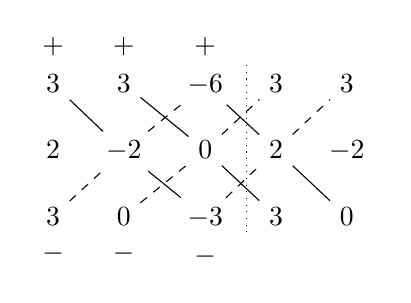
\begin{tikzpicture}
              \matrix [%
                matrix of math nodes,
                column sep=1em,
                row sep=1em
              ] (sarrus) {%
                3 & 3  & -6 & 3 & 3  \\
                2 & -2 & 0  & 2 & -2 \\
                3 & 0  & -3 & 3 & 0  \\
              };

              \path ($(sarrus-1-3.north east)+(0.5em,0)$) edge[dotted] ($(sarrus-3-3.south east)+(0.5em,0)$)
              (sarrus-1-1)                          edge         (sarrus-2-2)
              (sarrus-2-2)                          edge         (sarrus-3-3)
              (sarrus-1-2)                          edge         (sarrus-2-3)
              (sarrus-2-3)                          edge         (sarrus-3-4)
              (sarrus-1-3)                          edge         (sarrus-2-4)
              (sarrus-2-4)                          edge         (sarrus-3-5)
              (sarrus-3-1)                          edge[dashed] (sarrus-2-2)
              (sarrus-2-2)                          edge[dashed] (sarrus-1-3)
              (sarrus-3-2)                          edge[dashed] (sarrus-2-3)
              (sarrus-2-3)                          edge[dashed] (sarrus-1-4)
              (sarrus-3-3)                          edge[dashed] (sarrus-2-4)
              (sarrus-2-4)                          edge[dashed] (sarrus-1-5);

              \foreach \c in {1,2,3} {\node[anchor=south] at (sarrus-1-\c.north) {$+$};};
              \foreach \c in {1,2,3} {\node[anchor=north] at (sarrus-3-\c.south) {$-$};};
            \end{tikzpicture}
          \end{center}
          \sol{}
          \begin{flalign*}
            \vm{
            3 & 3                          & -6 \\
            2 & -2                         & 0  \\
            3 & 0                          & -3
            } & = 18 + 0 + 0 - 36 - 0 + 18      \\
              & = 0
          \end{flalign*}

    \item $\vm{
              5 & 7 & 1\\
              -3 & 6 & 9\\
              4 & 7 & 3
            }$
          \begin{center}
            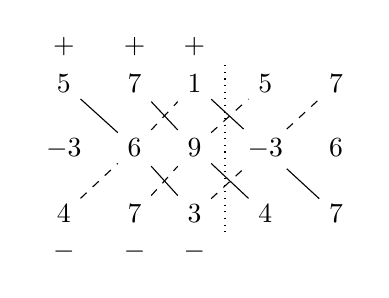
\begin{tikzpicture}
              \matrix [%
                matrix of math nodes,
                column sep=1em,
                row sep=1em
              ] (sarrus) {%
                5  & 7 & 1 & 5  & 7 \\
                -3 & 6 & 9 & -3 & 6 \\
                4  & 7 & 3 & 4  & 7 \\
              };

              \path ($(sarrus-1-3.north east)+(0.5em,0)$) edge[dotted] ($(sarrus-3-3.south east)+(0.5em,0)$)
              (sarrus-1-1)                          edge         (sarrus-2-2)
              (sarrus-2-2)                          edge         (sarrus-3-3)
              (sarrus-1-2)                          edge         (sarrus-2-3)
              (sarrus-2-3)                          edge         (sarrus-3-4)
              (sarrus-1-3)                          edge         (sarrus-2-4)
              (sarrus-2-4)                          edge         (sarrus-3-5)
              (sarrus-3-1)                          edge[dashed] (sarrus-2-2)
              (sarrus-2-2)                          edge[dashed] (sarrus-1-3)
              (sarrus-3-2)                          edge[dashed] (sarrus-2-3)
              (sarrus-2-3)                          edge[dashed] (sarrus-1-4)
              (sarrus-3-3)                          edge[dashed] (sarrus-2-4)
              (sarrus-2-4)                          edge[dashed] (sarrus-1-5);

              \foreach \c in {1,2,3} {\node[anchor=south] at (sarrus-1-\c.north) {$+$};};
              \foreach \c in {1,2,3} {\node[anchor=north] at (sarrus-3-\c.south) {$-$};};
            \end{tikzpicture}
          \end{center}
          \sol{}
          \begin{flalign*}
            \vm{
            5  & 7                               & 1 \\
            -3 & 6                               & 9 \\
            4  & 7                               & 3
            }  & = 90 + 252 - 21 - 24 - 315 + 63     \\
               & = 45
          \end{flalign*}

    \item $\vm{
              -2 & 7 & -4\\
              3 & -5 & 2\\
              -1 & 0 & -3
            }$
          \begin{center}
            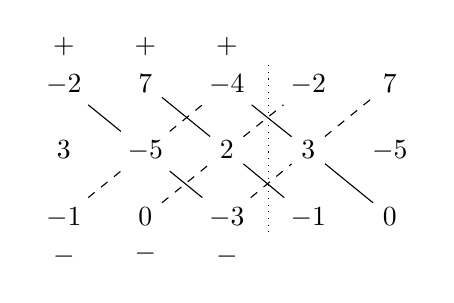
\begin{tikzpicture}
              \matrix [%
                matrix of math nodes,
                column sep=1em,
                row sep=1em
              ] (sarrus) {%
                -2 & 7  & -4 & -2 & 7  \\
                3  & -5 & 2  & 3  & -5 \\
                -1 & 0  & -3 & -1 & 0  \\
              };

              \path ($(sarrus-1-3.north east)+(0.5em,0)$) edge[dotted] ($(sarrus-3-3.south east)+(0.5em,0)$)
              (sarrus-1-1)                          edge         (sarrus-2-2)
              (sarrus-2-2)                          edge         (sarrus-3-3)
              (sarrus-1-2)                          edge         (sarrus-2-3)
              (sarrus-2-3)                          edge         (sarrus-3-4)
              (sarrus-1-3)                          edge         (sarrus-2-4)
              (sarrus-2-4)                          edge         (sarrus-3-5)
              (sarrus-3-1)                          edge[dashed] (sarrus-2-2)
              (sarrus-2-2)                          edge[dashed] (sarrus-1-3)
              (sarrus-3-2)                          edge[dashed] (sarrus-2-3)
              (sarrus-2-3)                          edge[dashed] (sarrus-1-4)
              (sarrus-3-3)                          edge[dashed] (sarrus-2-4)
              (sarrus-2-4)                          edge[dashed] (sarrus-1-5);

              \foreach \c in {1,2,3} {\node[anchor=south] at (sarrus-1-\c.north) {$+$};};
              \foreach \c in {1,2,3} {\node[anchor=north] at (sarrus-3-\c.south) {$-$};};
            \end{tikzpicture}
          \end{center}
          \sol{}
          \begin{flalign*}
            \vm{
            -2 & 7                            & -4 \\
            3  & -5                           & 2  \\
            -1 & 0                            & -3
            }  & = -30 - 14 - 0 + 20 + 0 + 63      \\
               & = -39
          \end{flalign*}

    \item $\vm{
              1 & 0 & -1\\
              3 & -2 & 5\\
              -1 & 1 & 3
            }$
          \sol{}
          \begin{flalign*}
            \vm{
            1  & 0                   & -1 \\
            3  & -2                  & 5  \\
            -1 & 1                   & 3
            }  & = \vm{
            -2 & 5                        \\
            1  & 3
            } -3 \vm{
            0  & -1                       \\
            1  & 3
            } - \vm{
            0  & -1                       \\
            -2 & 5
            }                             \\
               & = -11 - 3 + 2 = -12
          \end{flalign*}

    \item $\vm{
              2 & 6 & 4\\
              1 & 3 & 1\\
              -2 & -6 & 5
            }$
          \sol{}
          \begin{flalign*}
            \vm{
            2  & 6                                              & 4 \\
            1  & 3                                              & 1 \\
            -2 & -6                                             & 5
            }  & = 3\vm{
            2  & 2                                              & 4 \\
            1  & 1                                              & 1 \\
            -2 & -2                                             & 5
            }  &                                                    \\
               & = 0\ \ \ \ \ \text{(col 1 and 2 are the same)}     \\
          \end{flalign*}

    \item $\vm{
              10 & 8 & -2\\
              15 & 16 & -3\\
              -5 & -4 & 1
            }$
          \sol{}
          \begin{flalign*}
            \vm{
            10 & 8                                              & -2 \\
            15 & 16                                             & -3 \\
            -5 & -4                                             & 1
            }  & = -5\vm{
            2  & 8                                              & 2  \\
            3  & 16                                             & 3  \\
            -1 & -4                                             & -1
            }                                                        \\
               & = 0\ \ \ \ \ \text{(col 1 and 3 are the same)}
          \end{flalign*}

  \end{enumerate}

  \noindent Using the identities of determinant, prove the following equations (Question 23
  to 24):

  \begin{enumerate}[wide, labelwidth=!, labelindent=0pt]
    \setcounter{enumi}{22}

    \item $\vm{
              bc & 1 & bc(b+c)\\
              ca & 1 & ca(c+a)\\
              ab & 1 & ab(a+b)
            } = 0$
          \prooff{}
          \begin{flalign*}
               & \vm{
            bc & 1                              & bc(b+c)   \\
            ca & 1                              & ca(c+a)   \\
            ab & 1                              & ab(a+b)
            }                                               \\
               & = a^2b^2c^2\vm{
            1  & \frac{1}{bc}                   & b+c       \\
            1  & \frac{1}{ca}                   & c+a       \\
            1  & \frac{1}{ab}                   & a+b
            }                                               \\
               & = a^2b^2c^2\vm{
            1  & \frac{1}{bc}                   & -a        \\
            1  & \frac{1}{ca}                   & -b        \\
            1  & \frac{1}{ab}                   & -c
            }  & C_3 \rightarrow C_3+(a+b+c)C_1             \\
               & = a^2b^2c^2\vm{
            1  & a                              & -a        \\
            1  & b                              & -b        \\
            1  & c                              & -c
            }  & C_2 \rightarrow C_2 + abcC_1               \\
               & = -a^2b^2c^2\vm{
            1  & a                              & a         \\
            1  & b                              & b         \\
            1  & c                              & c
            }                                               \\
               & = 0                            & C_2 = C_3
          \end{flalign*}

    \item $\vm{
              a & 1 & a^2(b+c)\\
              b & 1 & b^2(c+a)\\
              c & 1 & c^2(a+b)
            } = 0$
          \prooff{}
          \begin{flalign*}
                  & \vm{
            a     & 1                                                     & a^2(b+c)            \\
            b     & 1                                                     & b^2(c+a)            \\
            c     & 1                                                     & c^2(a+b)
            }                                                                                   \\
                  & = \vm {
            a     & 1                                                     & a^2(b+c)            \\
            b - a & 0                                                     & b^2(c+a) - a^2(b+c) \\
            c - a & 0                                                     & c^2(a+b) - a^2(b+c)
            }                                                                                   \\
                  & R_2 \rightarrow R_2 - R_1,\ R_3 \rightarrow R_3 - R_1                       \\
                  & = \vm {
            b-a   & b^2(c+a) - a^2(b+c)                                                         \\
            c-a   & c^2(a+b) - a^2(b+c)
            }                                                                                   \\
                  & = (b-a)[c^2(a+b) - a^2(b+c)]                                                \\
                  & \ \ \ \ - (c-a)[b^2(c+a) - a^2(b+c)]                                        \\
                  & = c^2(b-a)(b+a) - a^2(b+c)(c-a)                                             \\
                  & \ \ \ \ - b^2(c-a)(c+a) + a^2(b+c)(c-a)                                     \\
                  & = c^2(b^2-a^2) - b^2(c^2-a^2)                                               \\
                  & = b^2c^2 - a^2c^2 - b^2c^2 + a^2c^2                                         \\
                  & = 0
          \end{flalign*}

  \end{enumerate}

  Find the value of $x$ in the following expressions (Question 25 to 26):

  \begin{enumerate}[wide, labelwidth=!, labelindent=0pt]
    \setcounter{enumi}{24}

    \item $\vm{
              2x & 3 & x+5\\
              -3 & 2 & 1\\
              2 & 1 & 0
            } = 5x - 1$
          \sol{}
          \begin{flalign*}
            \vm{
            2x                 & 3        & x+5 \\
            -3                 & 2        & 1   \\
            2                  & 1        & 0
            }                  & = 5x - 1       \\
            x+5\vm{
            -3                 & 2              \\
            2                  & 1
            } - \vm{
            2x                 & 3              \\
            2                  & 1
            }                  & = 5x - 1       \\
            -7(x+5) - (2x - 6) & = 5x - 1       \\
            -7x - 35 -2x + 6   & = 5x - 1       \\
            -14x               & = 28           \\
            x                  & = -2
          \end{flalign*}

    \item $\vm{
              x+3 & 1 & 0\\
              x & 3 & 0\\
              1 & 0 & -x-2
            } = x + 6$
          \sol{}
          \begin{flalign*}
            \vm{
            x+3             & 1                       & 0    \\
            x               & 3                       & 0    \\
            1               & 0                       & -x-2
            }               & = x + 6                        \\
            -x-2\vm{
            x+3             & 1                              \\
            x               & 3
            }               & = x + 6                        \\
            -(x+2)(3x+9-x)  & = x + 6                        \\
            (x+2)(2x+9)     & = -x-6                         \\
            2x^2 + 13x + 18 & = -x-6                         \\
            2x^2 + 14x + 24 & = 0                            \\
            x^2 + 7x + 12   & = 0                            \\
            (x+4)(x+3)      & = 0                            \\
            x               & = -4 \text{ or } x = -3
          \end{flalign*}

  \end{enumerate}

  \begin{enumerate}[wide, labelwidth=!, labelindent=0pt]
    \setcounter{enumi}{26}

    \item Given an identity matrix $I = \m{ 1 & 0\\ 0 & 1 }$. Let $J = \m{ 0 & 1\\ -1 & 0
            }$, ${(2I+J)}^{-1} = rI + sJ$, find the value of $r$ and $s$. \sol{}
          \begin{flalign*}
            {(2I+J)}^{-1}   & = {\left[2\m{
            1               & 0                                \\
            0               & 1
            } + \m{
            0               & 1                                \\
            -1              & 0
            }\right]}^{-1}                                     \\
                            & = {\left[\m{
            2               & 0                                \\
            0               & 2
            } + \m{
            0               & 1                                \\
            -1              & 0
            }\right]}^{-1}                                     \\
                            & = \m{
            2               & 1                                \\
            -1              & 2
            }^{-1}                                             \\
                            & = \frac{1}{5}\m{
            2               & -1                               \\
            1               & 2
            }                                                  \\
                            & = \m{
            \frac{2}{5}     & -\frac{1}{5}                     \\
            \frac{1}{5}     & \frac{2}{5}
            }                                                  \\
            rI + sJ         & = r\m{
            1               & 0                                \\
            0               & 1
            } + s\m{
            0               & 1                                \\
            -1              & 0
            }                                                  \\
                            & = \m{
            r               & 0                                \\
            0               & r
            } + \m{
            0               & s                                \\
            -s              & 0
            }                                                  \\
                            & = \m{
            r               & s                                \\
            -s              & r
            }                                                  \\
            {(2I + J)}^{-1} & = rI + sJ                        \\
            \m{
            \frac{2}{5}     & -\frac{1}{5}                     \\
            \frac{1}{5}     & \frac{2}{5}
            }               & = \m{
            r               & s                                \\
            -s              & r
            }                                                  \\
            \therefore\ r   & = \frac{2}{5},\ s = -\frac{1}{5}
          \end{flalign*}

  \end{enumerate}

  \noindent Find the value of $a$ in the following matrices if they are non-inversible (Question 28 to 31):

  \begin{enumerate}[wide, labelwidth=!, labelindent=0pt]
    \setcounter{enumi}{27}

    \item $\m{
              3 & a\\
              -2 & 6
            }$
          \sol{}
          \begin{flalign*}
            \vm{
            3       & a     \\
            -2      & 6
            }       & = 0   \\
            18 + 2a & = 0   \\
            2a      & = -18 \\
            a       & = -9
          \end{flalign*}

    \item $\m{
              5a + 2 & 4\\
              6 & a
            }$
          \sol{}
          \begin{flalign*}
            \vm{
            5a + 2                            & 4              \\
            6                                 & a
            }                                 & = 0            \\
            5a^2 + 2a - 24                    & = 0            \\
            (x-2)(5x + 12)                    & = 0            \\
            x               = 2 \text{ or } x & = \frac{12}{5}
          \end{flalign*}

    \item $\m{
              -7 & a & 3\\
              2 & -3 & 1\\
              0 & -a & 4
            }$
          \sol{}
          \begin{flalign*}
            \vm{
            -7                       & a    & 3 \\
            2                        & -3   & 1 \\
            0                        & -a   & 4
            }                        & = 0      \\
            -7\vm{
            -3                       & 1        \\
            -a                       & 4
            } - 2\vm{
            a                        & 3        \\
            -a                       & 4
            }                        & =0       \\
            -7(-12 + a) - 2(4a + 3a) & = 0      \\
            84 - 7a - 14a            & = 0      \\
            21a                      & = 84     \\
            a                        & = 4
          \end{flalign*}

    \item $\m{
              a & -1 & 0\\
              4 & 0 & -2\\
              a+4 & a & -8
            }$
          \sol{}
          \begin{flalign*}
            \vm{
            a                  & -1                     & 0  \\
            4                  & 0                      & -2 \\
            a+4                & a                      & -8
            }                  & = 0                         \\
            a\vm{
            0                  & -2                          \\
            a                  & -8
            } + \vm {
            4                  & -2                          \\
            a+4                & -8
            }                                                \\
            2a^2 - 32 + 2a + 8 & = 0                         \\
            2a^2 + 2a - 24     & = 0                         \\
            a^2 + a - 12       & = 0                         \\
            (a+4)(a-3)         & = 0                         \\
            a                  & = -4 \text{ or } a = 3
          \end{flalign*}

  \end{enumerate}

  \noindent Find the inverse of the following matrices (Question 32 to 37):

  \begin{enumerate}[wide, labelwidth=!, labelindent=0pt]
    \setcounter{enumi}{31}

    \item $\m{
              2 & 5\\
              2 & 3
            }$
          \sol{}
          \begin{flalign*}
            \m{
            2            & 5                 \\
            2            & 3
            }^{-1}       & = -\frac{1}{4}\m{
            3            & -5                \\
            -2           & 2
            }                                \\
                         & = \m{
            -\frac{3}{4} & \frac{5}{4}       \\
            \frac{1}{2}  & -\frac{1}{2}
            }
          \end{flalign*}

    \item $\m{
              -2 & -1 \\
              4 & 6
            }$
          \sol{}
          \begin{flalign*}
            \m{
            -2           & -1                \\
            4            & 6
            }^{-1}       & = -\frac{1}{8}\m{
            6            & 1                 \\
            -4           & -2
            }                                \\
                         & = \m{
            -\frac{3}{8} & -\frac{1}{8}      \\
            \frac{1}{2}  & \frac{1}{4}
            }
          \end{flalign*}

    \item $\m{
              1 & 0 & 3\\
              3 & 1 & 9\\
              -2 & 2 & -4
            }$
          \sol{}
          \begin{flalign*}
                & \vm{
            1   & 0                      & 3            \\
            3   & 1                      & 9            \\
            -2  & 2                      & -4
            }  = 2                                      \\
                & \operatorname{adj} \m{
            1   & 0                      & 3            \\
            3   & 1                      & 9            \\
            -2  & 2                      & -4
            }                                           \\
                & = \m{
            \vm{
            1   & 9                                     \\
            2   & -4
            }   & -\vm{
            3   & 9                                     \\
            -2  & -4
            }   & \vm{
            3   & 1                                     \\
            -2  & 2
            }                                           \\
            -\vm{
            0   & 3                                     \\
            2   & -4
            }   & \vm{
            1   & 3                                     \\
            -2  & -4
            }   & -\vm{
            1   & 0                                     \\
            -2  & 2
            }                                           \\
            \vm{
            0   & 3                                     \\
            1   & 9                                     \\
            }   & -\vm{
            1   & 3                                     \\
            3   & 9
            }   & \vm{
            1   & 0                                     \\
            3   & 1
            }
            }'                                          \\
                & =\m{
            -22 & -6                     & 8            \\
            6   & 2                      & -2           \\
            -3  & 0                      & 1
            }'                                          \\
                & = \m{
            -22 & 6                      & -3           \\
            -6  & 2                      & 0            \\
            8   & -2                     & 1
            }'                                          \\
                & \therefore\ \m{
            1   & 0                      & 3            \\
            3   & 1                      & 9            \\
            -2  & 2                      & -4
            }^{-1}                                      \\
                & = \frac{1}{2}\m{
            -22 & 6                      & -3           \\
            -6  & 2                      & 0            \\
            8   & -2                     & 1
            }                                           \\
                & = \m{
            -11 & 3                      & -\frac{3}{2} \\
            -3  & 1                      & 0            \\
            4   & -1                     & \frac{1}{2}
            }
          \end{flalign*}

    \item $\m{
              1 & 2 & -3\\
              2 & 1 & -4\\
              -2 & 5 & 1
            }$
          \sol{}
          \begin{flalign*}
                & \vm{
            1   & 2                      & -3           \\
            2   & 1                      & -4           \\
            -2  & 5                      & 1
            }  = -3                                     \\
                & \operatorname{adj} \m{
            1   & 2                      & -3           \\
            2   & 1                      & -4           \\
            -2  & 5                      & 1
            }                                           \\
                & = \m{
            \vm{
            1   & -4                                    \\
            5   & 1
            }   & -\vm{
            2   & -4                                    \\
            -2  & 1
            }   & \vm{
            2   & 1                                     \\
            -2  & 5
            }                                           \\
            -\vm{
            2   & -3                                    \\
            5   & 1
            }   & \vm{
            1   & -3                                    \\
            -2  & 1
            }   & -\vm{
            1   & 2                                     \\
            -2  & 5
            }                                           \\
            \vm{
            2   & -3                                    \\
            1   & -4                                    \\
            }   & -\vm{
            1   & -3                                    \\
            2   & -4
            }   & \vm{
            1   & 2                                     \\
            2   & 1
            }
            }'                                          \\
                & = \m{
            21  & 6                      & 12           \\
            -17 & -5                     & -9           \\
            -5  & -2                     & -3
            }'                                          \\
                & = \m{
            21  & -17                    & -5           \\
            6   & -5                     & -2           \\
            12  & -9                     & -3
            }'                                          \\
                & \therefore\ \m{
            1   & 2                      & -3           \\
            2   & 1                      & -4           \\
            -2  & 5                      & 1
            }^{-1}                                      \\
                & = -\frac{1}{3}\m{
            21  & -17                    & -5           \\
            6   & -5                     & -2           \\
            12  & -9                     & -3
            }                                           \\
                & = \m{
            -7  & -\frac{17}{3}          & -\frac{5}{3} \\
            -2  & -\frac{5}{3}           & -\frac{2}{3} \\
            -4  & 3                      & 1
            }
          \end{flalign*}

    \item $\m{
              4 & 1 & 0\\
              0 & -2 & 3\\
              0 & -4 & 4
            }$
          \sol{}
          \begin{flalign*}
                        & \vm{
            4           & 1                      & 0            \\
            0           & -2                     & 3            \\
            0           & -4                     & 4
            }  = 16                                             \\
                        & \operatorname{adj} \m{
            4           & 1                      & 0            \\
            0           & -2                     & 3            \\
            0           & -4                     & 4
            }                                                   \\
                        & = \m{
            \vm{
            -2          & 3                                     \\
            -4          & 4
            }           & -\vm{
            0           & 3                                     \\
            0           & 4
            }           & \vm{
            0           & -2                                    \\
            0           & -4
            }                                                   \\
            -\vm{
            1           & 0                                     \\
            -4          & 4
            }           & \vm{
            4           & 0                                     \\
            0           & 4
            }           & -\vm{
            4           & 1                                     \\
            0           & -4
            }                                                   \\
            \vm{
            1           & 0                                     \\
            -2          & 3
            }           & -\vm{
            4           & 0                                     \\
            0           & 3
            }           & \vm{
            4           & 1                                     \\
            0           & -2
            }
            }'                                                  \\
                        & = \m{
            4           & 0                      & 0            \\
            -4          & 16                     & 16           \\
            3           & -12                    & -8
            }'                                                  \\
                        & = \m{
            4           & -4                     & 0            \\
            0           & 16                     & -12          \\
            9           & 16                     & -8
            }                                                   \\
                        & \therefore\ \m{
            4           & 1                      & 0            \\
            0           & -2                     & 3            \\
            0           & -4                     & 4
            }^{-1}                                              \\
                        & = \frac{1}{16}\m{
            4           & -4                     & 3            \\
            0           & 16                     & -12          \\
            0           & 16                     & -8
            }                                                   \\
                        & = \m{
            \frac{1}{4} & -\frac{1}{4}           & \frac{3}{16} \\
            0           & 1                      & -\frac{3}{4} \\
            0           & 1                      & -\frac{1}{2}
            }
          \end{flalign*}

    \item $\m{
              3 & 2 & 4\\
              -1 & -3 & 0\\
              1 & 0 & 3
            }$
          \sol{}
          \begin{flalign*}
                         & \vm{
            3            & 2                      & 4            \\
            -1           & -3                     & 0            \\
            1            & 0                      & 3
            }  = -9                                              \\
                         & \operatorname{adj} \m{
            3            & 2                      & 4            \\
            -1           & -3                     & 0            \\
            1            & 0                      & 3
            }                                                    \\
                         & = \m{
            \vm{
            -3           & 0                                     \\
            0            & 3
            }            & -\vm{
            -1           & 0                                     \\
            1            & 3
            }            & \vm{
            -1           & -3                                    \\
            1            & 0
            }                                                    \\
            -\vm{
            2            & 4                                     \\
            0            & 3
            }            & \vm{
            3            & 4                                     \\
            1            & 3
            }            & -\vm{
            3            & 2                                     \\
            1            & 0
            }                                                    \\
            \vm{
            2            & 4                                     \\
            -3           & 0
            }            & -\vm{
            3            & 4                                     \\
            -1           & 0
            }            & \vm{
            3            & 2                                     \\
            -1           & -3
            }
            }'                                                   \\
                         & = \m{
            -9           & 3                      & 3            \\
            -6           & 5                      & 2            \\
            12           & -4                     & -7
            }'                                                   \\
                         & = \m{
            -9           & -6                     & 12           \\
            3            & 5                      & -4           \\
            3            & 2                      & -7
            }                                                    \\
                         & \therefore\ \m{
            3            & 2                      & 4            \\
            -1           & -3                     & 0            \\
            1            & 0                      & 3
            }                                                    \\
                         & = \frac{1}{-9}\m{
            -9           & -6                     & 12           \\
            3            & 5                      & -4           \\
            3            & 2                      & -7
            }                                                    \\
                         & = \m{
            -1           & \frac{2}{3}            & -\frac{4}{3} \\
            -\frac{1}{3} & -\frac{5}{9}           & \frac{4}{9}  \\
            -\frac{1}{3} & -\frac{2}{9}           & \frac{7}{9}
            }
          \end{flalign*}

  \end{enumerate}

  \noindent Solve the following system of equations using the method of Gauss elimination (Question 38 to 41):

  \begin{enumerate}[wide, labelwidth=!, labelindent=0pt]
    \setcounter{enumi}{37}

    \item $\begin{cases}
              2x - y + 4z = 5   \\
              2x + 3y - 4z = -7 \\
              x + y + z = 2
            \end{cases}$
          \sol{}
          \begin{flalign*}
                                                                               & \begin{amatrix}{3}
                                                                                   2 & -1 & 4 & 5\\
                                                                                   2 & 3 & -4 & -7\\
                                                                                   1 & 1 & 1 & 2
                                                                                 \end{amatrix}    \\
            \xrightarrow[R_1 \rightarrow R_1 + R_3]{R_2 \rightarrow R_2 + R_1} & \begin{amatrix}{3}
                                                                                   3 & 0 & 5 & 7\\
                                                                                   4 & 2 & 0 & -2\\
                                                                                   1 & 1 & 1 & 2
                                                                                 \end{amatrix}    \\
            \xrightarrow{R_2 \rightarrow \frac{1}{2}R_2}                       & \begin{amatrix}{3}
                                                                                   3 & 0 & 5 & 7\\
                                                                                   2 & 1 & 0 & -1\\
                                                                                   1 & 1 & 1 & 2
                                                                                 \end{amatrix}    \\
            \xrightarrow{R_3 \rightarrow R_3 - R_2}                            & \begin{amatrix}{3}
                                                                                   3 & 0 & 5 & 7\\
                                                                                   2 & 1 & 0 & -1\\
                                                                                   -1 & 0 & 1 & 3
                                                                                 \end{amatrix}    \\
            \xrightarrow{R_1 \rightarrow R_1 + 3R_3}                           & \begin{amatrix}{3}
                                                                                   0 & 0 & 8 & 16\\
                                                                                   2 & 1 & 0 & -1\\
                                                                                   -1 & 0 & 1 & 3
                                                                                 \end{amatrix}    \\
            \xrightarrow{R_1 \rightarrow \frac{1}{8}R_1}                       & \begin{amatrix}{3}
                                                                                   0 & 0 & 1 & 2\\
                                                                                   2 & 1 & 0 & -1\\
                                                                                   -1 & 0 & 1 & 3
                                                                                 \end{amatrix}    \\
            \xrightarrow{R_3 \rightarrow R_3 - R_1}                            & \begin{amatrix}{3}
                                                                                   0 & 0 & 1 & 2\\
                                                                                   2 & 1 & 0 & -1\\
                                                                                   -1 & 0 & 0 & 1
                                                                                 \end{amatrix}    \\
            \xrightarrow[R_3 \rightarrow -R3]{R_2 \rightarrow R_2 + 2R_3}      & \begin{amatrix}{3}
                                                                                   0 & 0 & 1 & 2\\
                                                                                   0 & 1 & 0 & 1\\
                                                                                   1 & 0 & 0 & -1
                                                                                 \end{amatrix}    \\
            \xrightarrow{R_1 \leftrightarrow R_2}                              & \begin{amatrix}{3}
                                                                                   1 & 0 & 0 & -1\\
                                                                                   0 & 1 & 0 & 1\\
                                                                                   0 & 0 & 1 & 2\\
                                                                                 \end{amatrix}    \\
            \therefore\ x                                                      & = -1,\ y = 1,\ z = 2
          \end{flalign*}

    \item $\begin{cases}
              x - 2y - 3z = -4 \\
              3x + y - 4z = -5 \\
              2x + 4y - z = -5
            \end{cases}$
          \sol{}
          \begin{flalign*}
                                                                                  & \begin{amatrix}{3}
                                                                                      1 & -2 & -3 & -4\\
                                                                                      3 & 1 & -4 & -5\\
                                                                                      2 & 4 & -1 & -5
                                                                                    \end{amatrix}    \\
            \xrightarrow[R_2 \rightarrow R_2 - 3R_1]{R_3 \rightarrow R_3 - 2R_1}  & \begin{amatrix}{3}
                                                                                      1 & -2 & -3 & -4\\
                                                                                      0 & 7 & 5 & 7\\
                                                                                      0 & 8 & 5 & 3
                                                                                    \end{amatrix}    \\
            \xrightarrow{R_3 \rightarrow R_3 - R_1}                               & = \begin{amatrix}{3}
                                                                                        1 & -2 & -3 & -4\\
                                                                                        0 & 7 & 5 & 7\\
                                                                                        0 & 1 & 0 & -4
                                                                                      \end{amatrix}  \\
            \xrightarrow[R_2 \rightarrow R_2 - 7R_3]{R_1 \rightarrow R_1 + 2R_3}  & = \begin{amatrix}{3}
                                                                                        1 & 0 & -3 & -12\\
                                                                                        0 & 0 & 5 & 35\\
                                                                                        0 & 1 & 0 & -4
                                                                                      \end{amatrix}  \\
            \xrightarrow[R_2 \leftrightarrow R_3]{R_2 \rightarrow \frac{1}{5}R_2} & = \begin{amatrix}{3}
                                                                                        1 & 0 & -3 & -12\\
                                                                                        0 & 1 & 0 & -4\\
                                                                                        0 & 0 & 1 & 7
                                                                                      \end{amatrix}  \\
            \xrightarrow{R_1 \rightarrow R_1 + 3R_2}                              & = \begin{amatrix}{3}
                                                                                        1 & 0 & 0 & 9\\
                                                                                        0 & 1 & 0 & -4\\
                                                                                        0 & 0 & 1 & 7
                                                                                      \end{amatrix}  \\
            \therefore\ x                                                         & = 9,\ y = -4,\ z = 7
          \end{flalign*}

    \item $\begin{cases}
              x - 2y - z = 3  \\
              4x - y + 2z = 1 \\
              x + 3y = 5
            \end{cases}$
          \sol{}
          \begin{flalign*}
                                                                                    & \begin{amatrix}{3}
                                                                                        1 & -2 & -1 & 3\\
                                                                                        4 & -1 & 2 & 1\\
                                                                                        1 & 3 & 0 & 5
                                                                                      \end{amatrix}    \\
            \xrightarrow[R_2 \rightarrow R_2 - 4R_3]{R_1 \rightarrow R_1 - R_3}     & \begin{amatrix}{3}
                                                                                        0 & -5 & -1 & -2\\
                                                                                        0 & -13 & 2 & -19\\
                                                                                        1 & 3 & 0 & 5
                                                                                      \end{amatrix}    \\
            \xrightarrow{R_2 \rightarrow R_2 + 2R_1}                                & \begin{amatrix}{3}
                                                                                        0 & -5 & -1 & -2\\
                                                                                        0 & -23 & 0 & -23\\
                                                                                        1 & 3 & 0 & 5
                                                                                      \end{amatrix}    \\
            \xrightarrow[R_1 \leftrightarrow R_3]{R_2 \rightarrow -\frac{1}{23}R_2} & \begin{amatrix}{3}
                                                                                        1 & 3 & 0 & 5\\
                                                                                        0 & 1 & 0 & 1\\
                                                                                        0 & -5 & -1 & -2
                                                                                      \end{amatrix}    \\
            \xrightarrow[R_3 \rightarrow R_3 + 5R_2]{R_1 \rightarrow R_1 - 3R_2}    & \begin{amatrix}{3}
                                                                                        1 & 0 & 0 & 2\\
                                                                                        0 & 1 & 0 & 1\\
                                                                                        0 & 0 & 1 & -3
                                                                                      \end{amatrix}    \\
            \therefore\ x                                                           & = 2,\ y = 1,\ z = -3
          \end{flalign*}

    \item $\begin{cases}
              2x - y - z = 0   \\
              4x - 3y + 2z = 1 \\
              3x - 2y - 4z = -1
            \end{cases}$
          \sol{}
          \begin{flalign*}
                                                                               & \begin{amatrix}{3}
                                                                                   2 & -1 & -1 & 0\\
                                                                                   4 & -3 & 2 & 1\\
                                                                                   3 & -2 & -4 & -1
                                                                                 \end{amatrix}                                 \\
            \xrightarrow{R_2 \rightarrow R_2 - 2R_1}                           & \begin{amatrix}{3}
                                                                                   2 & -1 & -1 & 0\\
                                                                                   0 & -1 & 4 & 1\\
                                                                                   3 & -2 & -4 & -1
                                                                                 \end{amatrix}                                 \\
            \xrightarrow[R_1 \rightarrow R_1 - R_2]{R_3 \rightarrow R_3 + R_2} & \begin{amatrix}{3}
                                                                                   2 & 0 & -5 & -1\\
                                                                                   0 & -1 & 4 & 1\\
                                                                                   3 & -3 & 0 & 0
                                                                                 \end{amatrix}                                 \\
            \xrightarrow{R_3 \rightarrow \frac{1}{3}R_3}                       & \begin{amatrix}{3}
                                                                                   2 & 0 & -5 & -1\\
                                                                                   0 & -1 & 4 & 1\\
                                                                                   1 & -1 & 0 & 0
                                                                                 \end{amatrix}                                 \\
            \xrightarrow{R_2 \rightarrow R_2 - R_3}                            & \begin{amatrix}{3}
                                                                                   2 & 0 & -5 & -1\\
                                                                                   -1 & 0 & 4 & 1\\
                                                                                   1 & -1 & 0 & 0
                                                                                 \end{amatrix}                                 \\
            \xrightarrow{R_1 \rightarrow R_1 + 2R_2}                           & \begin{amatrix}{3}
                                                                                   0 & 0 & 3 & 1\\
                                                                                   -1 & 0 & 4 & 1\\
                                                                                   1 & -1 & 0 & 0
                                                                                 \end{amatrix}                                 \\
            \xrightarrow{R_1 \rightarrow \frac{1}{3}R_1}                       & \begin{amatrix}{3}
                                                                                   0 & 0 & 1 & \frac{1}{3}\\
                                                                                   -1 & 0 & 4 & 1\\
                                                                                   1 & -1 & 0 & 0
                                                                                 \end{amatrix}                            \\
            \xrightarrow[R_3 \leftrightarrow R_2]{R_2 \rightarrow R_2 - 4R_1}  & \begin{amatrix}{3}
                                                                                   1 & -1 & 0 & 0\\
                                                                                   -1 & 0 & 0 & -\frac{1}{3}\\
                                                                                   0 & 0 & 1 & \frac{1}{3}\\
                                                                                 \end{amatrix}                          \\
            \xrightarrow{R_2 \rightarrow -R_2}                                 & \begin{amatrix}{3}
                                                                                   1 & -1 & 0 & 0\\
                                                                                   1 & 0 & 0 & \frac{1}{3}\\
                                                                                   0 & 0 & 1 & \frac{1}{3}\\
                                                                                 \end{amatrix}                            \\
            \xrightarrow{R_1 \rightarrow R_1 - R_2}                            & \begin{amatrix}{3}
                                                                                   0 & -1 & 0 & -\frac{1}{3}\\
                                                                                   1 & 0 & 0 & \frac{1}{3}\\
                                                                                   0 & 0 & 1 & \frac{1}{3}\\
                                                                                 \end{amatrix}                          \\
            \xrightarrow{R_1 \rightarrow -R_1}                                 & \begin{amatrix}{3}
                                                                                   0 & 1 & 0 & \frac{1}{3}\\
                                                                                   1 & 0 & 0 & \frac{1}{3}\\
                                                                                   0 & 0 & 1 & \frac{1}{3}\\
                                                                                 \end{amatrix}                            \\
            \xrightarrow{R_1 \leftrightarrow R_2}                              & \begin{amatrix}{3}
                                                                                   1 & 0 & 0 & \frac{1}{3}\\
                                                                                   0 & 1 & 0 & \frac{1}{3}\\
                                                                                   0 & 0 & 1 & \frac{1}{3}\\
                                                                                 \end{amatrix}                            \\
            \therefore\ x                                                      & = \frac{1}{3},\ y = \frac{1}{3},\ z = \frac{1}{3}
          \end{flalign*}

  \end{enumerate}

  \noindent Solve the following system of equations using the Cramer's rule (Question 42 to 45):

  \begin{enumerate}[wide, labelwidth=!, labelindent=0pt]
    \setcounter{enumi}{41}

    \item $\begin{cases}
              x - 3y - 2z = 1  \\
              7x + 4y - 5z = 0 \\
              3x + 9y + z = -1
            \end{cases}$
          \sol{}
          \begin{flalign*}
            \Delta        & = \vm{
            1             & -3                                                                    & -2 \\
            7             & 4                                                                     & -5 \\
            3             & 9                                                                     & 1
            }         = 13                                                                             \\
            \Delta_x      & = \vm{
            1             & -3                                                                    & -2 \\
            0             & 4                                                                     & -5 \\
            -1            & 9                                                                     & 1
            }         = 26                                                                             \\
            \Delta_y      & = \vm{
            1             & 1                                                                     & -2 \\
            7             & 0                                                                     & -5 \\
            3             & -1                                                                    & 1
            }         = -13                                                                            \\
            \Delta_z      & = \vm{
            1             & -3                                                                    & 1  \\
            7             & 4                                                                     & 0  \\
            3             & 9                                                                     & -1
            }         = 26                                                                             \\
            \therefore\ x & = \frac{26}{13} = 2,\ y = \frac{-13}{13} = -1,\ z = \frac{26}{13} = 2
          \end{flalign*}

    \item $\begin{cases}
              x - 2y + 3z = 6   \\
              2x + 3y - 4z = 20 \\
              3x - 2y - 5z = 6
            \end{cases}$
          \sol{}
          \begin{flalign*}
            \Delta        & = \vm{
            1             & -2                                                                           & 3  \\
            2             & 3                                                                            & -4 \\
            3             & -2                                                                           & -5
            } = -58                                                                                           \\
            \Delta_x      & = \vm{
            6             & -2                                                                           & 3  \\
            20            & 3                                                                            & -4 \\
            6             & -2                                                                           & -5
            } = -464                                                                                          \\
            \Delta_y      & = \vm{
            1             & 6                                                                            & 3  \\
            2             & 20                                                                           & -4 \\
            3             & 6                                                                            & -5
            } = -232                                                                                          \\
            \Delta_z      & = \vm{
            1             & -2                                                                           & 6  \\
            2             & 3                                                                            & 20 \\
            3             & -2                                                                           & 6
            } = -116                                                                                          \\
            \therefore\ x & = \frac{-464}{-58} = 8,\ y = \frac{-232}{-58} = 4,\ z = \frac{-116}{-58} = 2
          \end{flalign*}

    \item $\begin{cases}
              2x - 2y - 4z + 3 = 0 \\
              2x + 3y + 4z - 2 = 0 \\
              7x + 3y - 2z - 2 = 0
            \end{cases}$
          \sol{}
          \begin{flalign*}
                          & \begin{cases}
                              2x - 2y - 4z = -3 \\
                              2x + 3y + 4z = 2  \\
                              7x + 3y - 2z = 2
                            \end{cases}                                                             \\
            \Delta        & = \vm{
            2             & -2                                                                                            & -4 \\
            2             & 3                                                                                             & 4  \\
            7             & 3                                                                                             & -2
            } = -40                                                                                                            \\
            \Delta_x      & = \vm{
            -3            & -2                                                                                            & -4 \\
            2             & 3                                                                                             & 4  \\
            2             & 3                                                                                             & -2
            } = 30                                                                                                             \\
            \Delta_y      & = \vm{
            2             & -3                                                                                            & -4 \\
            2             & 2                                                                                             & 4  \\
            7             & 2                                                                                             & -2
            } = -80                                                                                                            \\
            \Delta_z      & = \vm{
            2             & -2                                                                                            & -3 \\
            2             & 3                                                                                             & 2  \\
            7             & 3                                                                                             & 2
            } = 25                                                                                                             \\
            \therefore\ x & = \frac{30}{-40} = -\frac{3}{4},\ y = \frac{-80}{-40} = 2,\ z = \frac{25}{-40} = -\frac{5}{8}
          \end{flalign*}

    \item $\begin{cases}
              \frac{2}{x} - \frac{5}{y} + \frac{4}{z} = -3 \\
              \frac{4}{x} + \frac{1}{y} - \frac{2}{z} = 7  \\
              \frac{7}{x} - \frac{3}{z} = 4
            \end{cases}$
          \sol{}
          \begin{flalign*}
            \text{Let }   & a = \frac{1}{x},\ b = \frac{1}{y},\ c = \frac{1}{z}                                                    \\
                          & \begin{cases}
                              2a - 5b + 4c = -3 \\
                              4a + b - 2c = 7   \\
                              7a - 3c = 4
                            \end{cases}                                                                 \\
            \Delta        & = \vm{
            2             & -5                                                                                                & 4  \\
            4             & 1                                                                                                 & -2 \\
            7             & 0                                                                                                 & -3
            } = -24                                                                                                                \\
            \Delta_a      & = \vm{
            -3            & -5                                                                                                & 4  \\
            7             & 1                                                                                                 & -2 \\
            4             & 0                                                                                                 & -3
            } = -72                                                                                                                \\
            \Delta_b      & = \vm{
            2             & -3                                                                                                & 4  \\
            4             & 7                                                                                                 & -2 \\
            7             & 4                                                                                                 & -3
            } = -152                                                                                                               \\
            \Delta_c      & = \vm{
            2             & -5                                                                                                & -3 \\
            4             & 1                                                                                                 & 7  \\
            7             & 0                                                                                                 & 4
            } = -136                                                                                                               \\
            \therefore\ a & = \frac{-72}{-24} = 3,\ b = \frac{-152}{-24} = \frac{19}{3},\ c = \frac{-136}{-24} = \frac{17}{3}      \\
            \therefore\ x & = \frac{1}{3},\ y = \frac{3}{19},\ z = \frac{3}{17}
          \end{flalign*}

  \end{enumerate}

  \chapter{Inequalities and Linear Programming}

  \section{Inequalities and its Identities}

  \subsection*{Inequalities}

  An inequality is a relation which makes a non-equal comparison between two
  numbers or other mathematical expressions. For example: \makeatletter
  \setbool{@fleqn}{false} \makeatother
  \begin{flalign*}
    11 > 10 \\
    x^2 + 5 < 6x
  \end{flalign*}
  \makeatletter
  \setbool{@fleqn}{true}
  \makeatother

  \begin{itemize}
    \item $a < b$ means $a$ is lesser than $b$
    \item $a > b$ means $a$ is greater than $b$
    \item $a \leq b$ means $a$ is lesser than or equal to $b$
    \item $a \geq b$ means $a$ is greater than or equal to $b$
  \end{itemize}

  \noindent For any real number $a$ and $b$, the following are true:
  \begin{enumerate}
    \item If $a - b > 0$, then $a > b$
    \item If $a - b < 0$, then $a < b$
  \end{enumerate}
  That means, if we want to compare between two numbers, we just have to calculate their difference.

  \subsection{Practice 1}

  Compare the following algebraic expressions:

  \begin{enumerate}
    \item $(x+3)(x-1)$ and $(x+4)(x-2)$
          \sol{}
          \begin{flalign*}
                         & (x+3)(x-1) - (x+4)(x-2)         \\
                         & = x^2 + 2x - 3 - (x^2 + 2x - 8) \\
                         & = x^2 + 2x - 3 - x^2 - 2x + 8   \\
                         & = 5 > 0                         \\
            \therefore\  & (x+3)(x-1) > (x+4)(x-2)
          \end{flalign*}

    \item $(x+8)(x+10)$ and ${(x+9)}^2$
          \sol{}
          \begin{flalign*}
                         & (x+8)(x+10) - {(x+9)}^2             \\
                         & = x^2 + 18x + 80 - (x^2 + 18x + 81) \\
                         & = x^2 + 18x + 80 - x^2 - 18x - 81   \\
                         & = -1 < 0                            \\
            \therefore\  & (x+8)(x+10) < {(x+9)}^2
          \end{flalign*}

    \item $x^2 + 6x$ and $4x-2$
          \sol{}
          \begin{flalign*}
                         & x^2 + 6x - 4x + 2     \\
                         & = x^2 + 2x + 2        \\
                         & = {(x + 1)}^2 - 1 + 2 \\
                         & = {(x + 1)}^2 + 1     \\
            \because\    & {(x+1)}^2 > 0         \\
            \therefore\  & {(x+1)}^2 + 1 > 0     \\
            \therefore\  & x^2 + 6x > 4x - 2
          \end{flalign*}
  \end{enumerate}

  \subsection*{Identities of Inequalities}

  \setcounter{theorem}{0}
  \begin{theorem}
    If $a > b$, $b > c$, then $a > c$
  \end{theorem}
  \begin{theorem}
    If $a > b$ then $a + c > b + c$
  \end{theorem}
  \begin{theorem}
    If $a > b$, $c > d$, then $a + c > b + d$
  \end{theorem}
  \begin{theorem}
    If $a > b$, then:
    \begin{enumerate}
      \item When $c > 0$, $ac > bc$
      \item When $c = 0$, $ac = bc$
      \item When $c < 0$, $ac < bc$
    \end{enumerate}
  \end{theorem}

  \subsection{Practice 2}

  Given that $y < x < 0$, use inequality signs to complete the following
  statements:

  \begin{enumerate}
    \item $x+1$ and $y+1$
          \sol{}
          \begin{flalign*}
            \because\    & y < x     \\
            \therefore\  & y+1 < x+1
          \end{flalign*}

    \item $2y$ and $2x$
          \sol{}
          \begin{flalign*}
            \because\    & y < x,\ 2 > 0 \\
            \therefore\  & 2y < 2x
          \end{flalign*}

    \item $-x + 1$ and $-y + 2$
          \sol{}
          \begin{flalign*}
            \because\    & y < x           \\
            \therefore\  & -x < -y         \\
            \because\    & 1 < 2,\ -x < -y \\
            \therefore\  & -x + 1 < -y + 2
          \end{flalign*}

    \item $3x$ and $4y$
          \sol{}
          \begin{flalign*}
            \because\    & y < x                      \\
            \therefore\  & 3y < 3x       & \cdots (1) \\
            and,\        & y < 0         & \cdots (2) \\
            (1) + (2):   & \ 3y + y < 3x              \\
                         & \ 4y < 3x
          \end{flalign*}
  \end{enumerate}

  \subsection{Exercise 15.1}

  Compare the following algebraic expressions (Question 1 to 5):

  \begin{enumerate}[wide, labelwidth=!, labelindent=0pt]

    \item ${(x-4)}^2$ and $(x-6)(x-2)$
          \sol{}
          \begin{flalign*}
                         & {(x-4)}^2 - (x-6)(x-2)            \\
                         & = x^2 - 8x + 16 - (x^2 - 8x + 12) \\
                         & = x^2 - 8x + 16 - x^2 + 8x - 12   \\
                         & = 4 > 0                           \\
            \therefore\  & {(x-4)}^2 > (x-6)(x-2)
          \end{flalign*}

    \item $x^2 + 13$ and $4x$
          \sol{}
          \begin{flalign*}
                         & x^2 + 13 - 4x        \\
                         & = x^2 - 4x + 13      \\
                         & = {(x-2)}^2 - 4 + 13 \\
                         & = {(x-2)}^2 + 9      \\
            \because\    & {(x-2)}^2 > 0        \\
            \therefore\  & {(x-2)}^2 + 9 > 0    \\
            \therefore\  & x^2 + 13 > 4x
          \end{flalign*}
    \item $(x-1)(x^2 + x + 1)$ and $(x+1)(x^2 - x + 1)$
          \sol{}
          \begin{flalign*}
                         & (x-1)(x^2 + x + 1) - (x+1)(x^2 - x + 1) \\
                         & = x^3 - 1 - x^3 - 1                     \\
                         & = -2 < 0                                \\
            \therefore\  & (x-1)(x^2 + x + 1) < (x+1)(x^2 - x + 1)
          \end{flalign*}

    \item $(x^2 - x + 1)(x^2 + x + 1)$ and $x^4 + x^2 - 1$
          \sol{}
          \begin{flalign*}
                         & (x^2 - x + 1)(x^2 + x + 1) - x^4 - x^2 + 1                      & \\
                         & = x^4 + x^3 + x^2 - x^3 - x^2 - x + x^2 + x + 1 - x^4 - x^2 + 1 & \\
                         & = 2 > 0                                                         & \\
            \therefore\  & (x^2 - x + 1)(x^2 + x + 1) > x^4 + x^2 - 1
          \end{flalign*}

    \item $(1 - 2x)(1 + 2x)$ and ${(x^2 - 6)}^2$
          \sol{}
          \begin{flalign*}
                         & {(x^2 - 6)}^2 - (1 - 2x)(1 + 2x) \\
                         & = x^4 - 12x^2 + 36 - 1 + 4x^2    \\
                         & = x^4 - 8x^2 + 35                \\
                         & = {(x^2 - 4)}^2 - 16 + 35        \\
                         & = {(x^2 - 4)}^2 + 19             \\
            \because\    & {(x^2 - 4)}^2 > 0                \\
            \therefore\  & {(x^2 - 4)}^2 + 19 > 0           \\
            \therefore\  & {(x^2 - 6)}^2 > (1 - 2x)(1 + 2x) \\
          \end{flalign*}

    \item Given that $y < x < 0$, use inequality signs to complete the following:
          \begin{enumerate}

            \item $2x - 3$ and $2y - 5$
                  \sol{}
                  \begin{flalign*}
                    \because\    & y < x,\ 2 > 0     \\
                    \therefore\  & 2y < 2x           \\
                    \because\    & -3 > -5,\ 2x > 2y \\
                    \therefore\  & 2x - 3 > 2y - 5
                  \end{flalign*}

            \item $x^2$ and $y^2$
                  \sol{}
                  \begin{flalign*}
                    \because\    & y < x,\ x^2 > 0,\ y^2 > 0 \\
                    \therefore\  & y^2 < x^2
                  \end{flalign*}

          \end{enumerate}

  \end{enumerate}

  \section{Linear Inequalities}

  \subsection*{Solving Linear Inequalities}

  The general form of a linear inequality is $ax + b \leq c$, where $a \neq 0$.

  \subsection{Practice 3}

  Solve the following linear inequalities:

  \begin{enumerate}
    \item $2x > x + 9$
          \sol{}
          \begin{flalign*}
            2x & > x + 9 \\
            x  & > 9
          \end{flalign*}

    \item $11 - 2x \leq -7$
          \sol{}
          \begin{flalign*}
            11 - 2x & \leq -7  \\
            -2x     & \leq -18 \\
            2x      & \geq 18  \\
            x       & \geq 9
          \end{flalign*}

    \item $2(x + 2) \geq \frac{2}{3} + \frac{2x+3}{4}$
          \sol{}
          \begin{flalign*}
            2(x + 2) & \geq \frac{2}{3} + \frac{2x+3}{4} \\
            2x + 4   & \geq \frac{2}{3} + \frac{2x+3}{4} \\
            24x + 48 & \geq 8 + 6x + 9                   \\
            24x + 48 & \geq 17 + 6x                      \\
            18x      & \geq -31                          \\
            x        & \geq -\frac{31}{18}
          \end{flalign*}

    \item $2x - \frac{x}{3} + \frac{1}{3} < 3x - \frac{1}{2} + \frac{x}{6}$
          \sol{}
          \begin{flalign*}
            2x - \frac{x}{3} + \frac{1}{3} & < 3x - \frac{1}{2} + \frac{x}{6} \\
            12x - 2x + 2                   & < 18x - 3 + x                    \\
            10x + 2                        & < 19x - 3                        \\
            -9x                            & < -5                             \\
            x                              & > \frac{5}{9}
          \end{flalign*}

    \item $10 \leq x + 3 \leq 12$
          \sol{}
          \begin{flalign*}
            10 & \leq x + 3 \leq 12  \\
            7  & \leq x       \leq 9
          \end{flalign*}

    \item $-3 < 7 - 2x < 9$
          \sol{}
          \begin{flalign*}
            -3  & < 7 - 2x < 9 \\
            -10 & < -2x < 2    \\
            -2  & < 2x < 10    \\
            -1  & < x < 5
          \end{flalign*}
  \end{enumerate}

  \subsection{Exercise 15.2a}

  Solve the following linear inequalities:

  \begin{enumerate}
    \item $4x - 3 > x + 9$
          \sol{}
          \begin{flalign*}
            4x - 3 & > x + 9 \\
            3x     & > 12    \\
            x      & > 4
          \end{flalign*}

    \item $-4x > 1 - x$
          \sol{}
          \begin{flalign*}
            -4x & > 1 - x \\
            -3x > 1       \\
            3x < -1       \\
            x < -\frac{1}{3}
          \end{flalign*}

    \item $3x + 20 \geq 34 - 4x$
          \sol{}
          \begin{flalign*}
            7x & \geq 14 \\
            7x & \geq 14 \\
          \end{flalign*}

    \item $5x + 8 \leq 6x - 7$
          \sol{}
          \begin{flalign*}
            5x + 8 & \leq 6x - 7 \\
            -x \leq -15          \\
            x \geq 15
          \end{flalign*}
    \item $1 \leq 6(x-7)$
          \sol{}
          \begin{flalign*}
            1  & \leq 6(x-7)       \\
            1  & \leq 6x - 42      \\
            6x & \geq 43           \\
            x  & \geq \frac{43}{6}
          \end{flalign*}
    \item $2(x+7) \leq 5x + 14$
          \sol{}
          \begin{flalign*}
            2(x+7)  & \leq 5x + 14 \\
            2x + 14 & \leq 5x + 14 \\
            -3x     & \leq 0       \\
            x       & \geq 0
          \end{flalign*}

    \item $\frac{x}{2} + \frac{2 - 3x}{5} > -\frac{7}{2} + \frac{x+1}{5}$
          \sol{}
          \begin{flalign*}
            \frac{x}{2} + \frac{2 - 3x}{5} & > -\frac{7}{2} + \frac{x+1}{5} \\
            5x + 4 - 6x                    & > -35 + 2x + 2                 \\
            -x + 4                         & > -33 + 2x                     \\
            -3x                            & > -37                          \\
            x                              & < \frac{37}{3}
          \end{flalign*}

    \item $-5 < 12 - x < -1$
          \sol{}
          \begin{flalign*}
            -5  & < 12 - x < -1 \\
            -17 & < -x < -13    \\
            13  & < x < 17
          \end{flalign*}

    \item $-\frac{3}{5} < \frac{x}{2} - \frac{1}{2} < \frac{2}{5}$
          \sol{}
          \begin{flalign*}
            -6           & < 5x - 5 < 4      \\
            -1           & < 5x < 9          \\
            -\frac{1}{5} & < x < \frac{9}{5}
          \end{flalign*}

    \item $-2 < \frac{2x}{3} + \frac{1}{2} \leq 4$
          \sol{}
          \begin{flalign*}
            -12           & < 4x + 3 \leq 24      \\
            -15           & < 4x \leq 21          \\
            -\frac{15}{4} & < x \leq \frac{21}{4}
          \end{flalign*}
  \end{enumerate}

  \subsection*{Solution of the System of Linear Inequalities}

  The system of iniqualities formed by more than one linear inequality is called
  a system of linear inequalities. The solution of a system of linear
  inequalities is the set of all points that satisfy all the inequalities in the
  system, and can be represented by a numberline.

  \subsection{Practice 4}

  Solve the following system of linear inequalities.

  \begin{enumerate}
    \setcounter{equation}{0}
    \item \begin{numcases}{}
            3x +2 \geq{} 2x -2 \\
            4x -3 > 3x -2
          \end{numcases}
          \sol{}
          \begin{flalign*}
            (1)          : x & \geq{} 4 \\
            (2)          : x & > 1      \\
            \\
            \therefore\  x   & > 1
          \end{flalign*}
          \begin{center}
            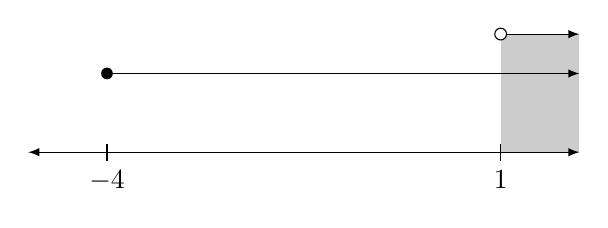
\begin{tikzpicture}
              \fill[black!20](1,0)rectangle(2,1.5);
              \draw[latex-latex] (-5,0) -- (2,0) ;
              \foreach \x in {-4, 1} \draw[shift={(\x,0)},color=black] (0pt,3pt) -- (0pt,-3pt) node[below] {$\x$};
              \node[circle,fill,inner sep=1.5pt](a)at(-4,1){};
              \node[circle,draw,fill=white,inner sep=1.5pt](b)at(1,1.5){};
              \draw[-latex,black](a)--(2,1);
              \draw[-latex,black](b)--(2,1.5);
            \end{tikzpicture}
          \end{center}

          \setcounter{equation}{0}
    \item \begin{numcases}{}
            5x -4 \leq{} 2x + 5\\
            7 -x < 3 + x
          \end{numcases}
          \sol{}
          \begin{flalign*}
            (1) : 3x       & \leq{} 9     \\
            x              & \leq{} 3     \\
            (2) : -2x      & < -4         \\
            x              & > 2          \\
            \\
            \therefore\  2 & < x \leq{} 3
          \end{flalign*}
          \begin{center}
            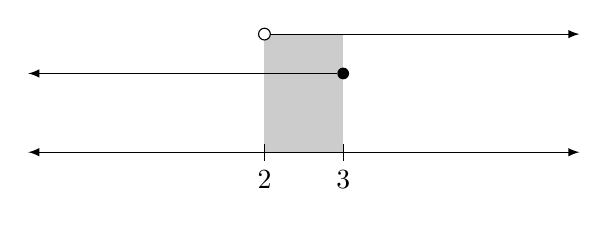
\begin{tikzpicture}
              \fill[black!20](2,0)rectangle(3,1.5);
              \draw[latex-latex] (-1,0) -- (6,0) ;
              \foreach \x in {2, 3} \draw[shift={(\x,0)},color=black] (0pt,3pt) -- (0pt,-3pt) node[below] {$\x$};
              \node[circle,fill,inner sep=1.5pt](a)at(3,1){};
              \node[circle,draw,fill=white,inner sep=1.5pt](b)at(2,1.5){};
              \draw[-latex,black](a)--(-1,1);
              \draw[-latex,black](b)--(6,1.5);
            \end{tikzpicture}
          \end{center}

          \setcounter{equation}{0}
    \item \begin{numcases}{}
            2 -x < 4 + x\\
            1 -2x \geq{} 3x + 11
          \end{numcases}
          \sol{}
          \begin{flalign*}
            (1) : -2x    & < 2                \\
            x            & > -1               \\
            (2) : -5x    & \geq{} 10          \\
            x            & \leq{} -2          \\
            \\
            \therefore\  & \text{No solution}
          \end{flalign*}
          \begin{center}
            \begin{tikzpicture}
              \draw[latex-latex] (-5,0) -- (2,0) ;
              \foreach \x in {-2, -1} \draw[shift={(\x,0)},color=black] (0pt,3pt) -- (0pt,-3pt) node[below] {$\x$};
              \node[circle,fill,inner sep=1.5pt](a)at(-2,1){};
              \node[circle,draw,fill=white,inner sep=1.5pt](b)at(-1,1){};
              \draw[-latex,black](a)--(-5,1);
              \draw[-latex,black](b)--(2,1);
            \end{tikzpicture}
          \end{center}

    \item $2-x < 2x-7 \leq{} x-9$
          \sol{}
          \setcounter{equation}{0}
          \begin{numcases}{}
            2-x < 2x-7 \\
            2x-7 \leq{} x-9
          \end{numcases}
          \begin{flalign*}
            (1) : -3x    & < -9               \\
            x            & \geq{} 3           \\
            (2) : x      & \leq{} -2          \\
            \\
            \therefore\  & \text{No solution}
          \end{flalign*}
          \begin{center}
            \begin{tikzpicture}
              \draw[latex-latex] (-3,0) -- (4,0) ;
              \foreach \x in {-2, 3} \draw[shift={(\x,0)},color=black] (0pt,3pt) -- (0pt,-3pt) node[below] {$\x$};
              \node[circle,fill,inner sep=1.5pt](a)at(-2,1){};
              \node[circle,draw,fill=white,inner sep=1.5pt](b)at(3,1){};
              \draw[-latex,black](a)--(-3,1);
              \draw[-latex,black](b)--(4,1);
            \end{tikzpicture}
          \end{center}
  \end{enumerate}

  \subsection{Exercise 15.2b}

  Solve the following system of linear inequalities.

  \begin{enumerate}

    \setcounter{equation}{0}
    \item \begin{numcases}{}
            5 -x < 6\\
            7 -3x \geq{} 4
          \end{numcases}
          \sol{}
          \begin{flalign*}
            (1) : -x        & < 1          \\
            x               & > -1         \\
            (2) : -3x       & \geq{} -3    \\
            x               & \leq{} 1     \\
            \\
            \therefore\  -1 & < x \leq{} 1
          \end{flalign*}
          \begin{center}
            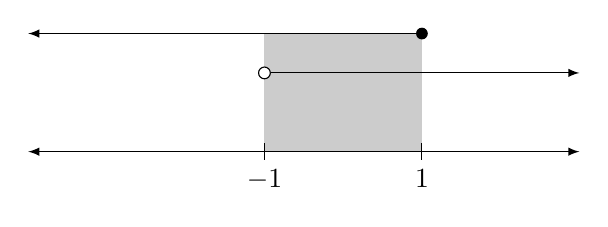
\begin{tikzpicture}
              \fill[black!20](-1,0)rectangle(1,1.5);
              \draw[latex-latex] (-4,0) -- (3,0) ;
              \foreach \x in {-1, 1} \draw[shift={(\x,0)},color=black] (0pt,3pt) -- (0pt,-3pt) node[below] {$\x$};
              \node[circle,fill,inner sep=1.5pt](a)at(1,1.5){};
              \node[circle,draw,fill=white,inner sep=1.5pt](b)at(-1,1){};
              \draw[-latex,black](a)--(-4,1.5);
              \draw[-latex,black](b)--(3,1);
            \end{tikzpicture}
          \end{center}

          \setcounter{equation}{0}
    \item \begin{numcases}{}
            x + 2 > 0\\
            2x + 1 \leq{} 4x -3
          \end{numcases}
          \sol{}
          \begin{flalign*}
            (1) : x        & > -2      \\
            (2) : -2x      & \leq{} -4 \\
            x              & \geq{} 2  \\
            \\
            \therefore\  x & \geq{} 2
          \end{flalign*}
          \begin{center}
            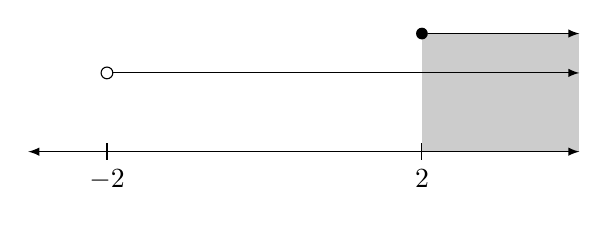
\begin{tikzpicture}
              \fill[black!20](2,0)rectangle(4,1.5);
              \draw[latex-latex] (-3,0) -- (4,0) ;
              \foreach \x in {-2, 2} \draw[shift={(\x,0)},color=black] (0pt,3pt) -- (0pt,-3pt) node[below] {$\x$};
              \node[circle,fill,inner sep=1.5pt](a)at(2,1.5){};
              \node[circle,draw,fill=white,inner sep=1.5pt](b)at(-2,1){};
              \draw[-latex,black](a)--(4,1.5);
              \draw[-latex,black](b)--(4,1);
            \end{tikzpicture}
          \end{center}

          \setcounter{equation}{0}
    \item \begin{numcases}{}
            3x -1 < 0\\
            1 -2x \geq{} 0
          \end{numcases}
          \sol{}
          \begin{flalign*}
            (1) : 3x       & < 1                \\
            x              & < \frac{1}{3}      \\
            (2) : -2x      & \geq{} -1          \\
            x              & \leq{} \frac{1}{2} \\
            \\
            \therefore\  x & < \frac{1}{3}
          \end{flalign*}
          \begin{center}
            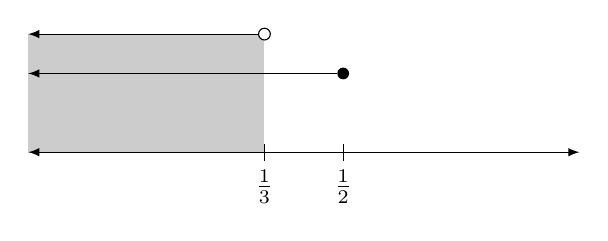
\begin{tikzpicture}
              \fill[black!20](-6,0)rectangle(-3,1.5);
              \draw[latex-latex] (-6,0) -- (1,0) ;
              \foreach \x in {2, 3} \draw[shift={(-\x,0)},color=black] (0pt,3pt) -- (0pt,-3pt) node[below] {$\frac{1}{\x}$};
              \node[circle,fill,inner sep=1.5pt](a)at(-2,1){};
              \node[circle,draw,fill=white,inner sep=1.5pt](b)at(-3,1.5){};
              \draw[-latex,black](a)--(-6,1);
              \draw[-latex,black](b)--(-6,1.5);
            \end{tikzpicture}
          \end{center}

          \setcounter{equation}{0}
    \item \begin{numcases}{}
            4x -6 \geq{} 5x\\
            3x + 5 \leq{} x + 9
          \end{numcases}
          \sol{}
          \begin{flalign*}
            (1) : -x       & \geq{} 6  \\
            x              & \leq{} -6 \\
            (2) : 2x       & \leq{} 4  \\
            x              & \geq{} 2  \\
            \\
            \therefore\  x & \leq{} -6
          \end{flalign*}
          \begin{center}
            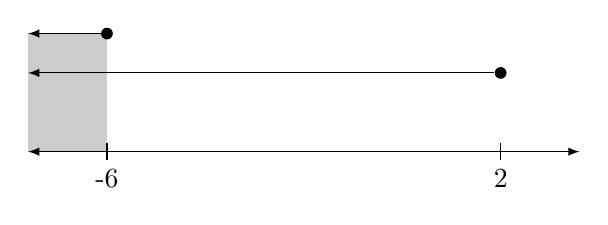
\begin{tikzpicture}
              \fill[black!20](-7,0)rectangle(-6,1.5);
              \draw[latex-latex] (-7,0) -- (0,0) ;
              \draw[shift={(-6,0)},color=black] (0pt,3pt) -- (0pt,-3pt) node[below] {-6};
              \draw[shift={(-1,0)},color=black] (0pt,3pt) -- (0pt,-3pt) node[below] {2};
              \node[circle,fill,inner sep=1.5pt](a)at(-6,1.5){};
              \node[circle,fill,inner sep=1.5pt](b)at(-1,1){};
              \draw[-latex,black](a)--(-7,1.5);
              \draw[-latex,black](b)--(-7,1);
            \end{tikzpicture}
          \end{center}

          \setcounter{equation}{0}
    \item \begin{numcases}{}
            2(x+2) > 3x\\
            6x -8 > 4(x+1)
          \end{numcases}
          \sol{}
          \begin{flalign*}
            (1): 2x + 4  & > 3x               \\
            -x           & > -4               \\
            x            & < 4                \\
            (2): 6x -  8 & > 4x + 4           \\
            2x           & > 12               \\
            x            & > 6                \\
            \\
            \therefore\  & \text{No solution}
          \end{flalign*}
          \begin{center}
            \begin{tikzpicture}
              \draw[latex-latex] (2,0) -- (9,0);
              \foreach \x in {4, 6} \draw[shift={(\x,0)},color=black] (0pt,3pt) -- (0pt,-3pt) node[below] {$\x$};
              \node[circle,fill,inner sep=1.5pt](a)at(4,1){};
              \node[circle,fill,inner sep=1.5pt](b)at(6,1){};
              \draw[-latex,black](a)--(2,1);
              \draw[-latex,black](b)--(9,1);
            \end{tikzpicture}
          \end{center}

          \setcounter{equation}{0}
    \item \begin{numcases}{}
            4x + 4 \leq{} 3x + 7\\
            \frac{5x}{2} -1 \leq{} 3x -2
          \end{numcases}
          \sol{}
          \begin{flalign*}
            (1): x        & \leq{} 3          \\
            (2): 5x - 2   & \leq{} 6x - 4     \\
            -x            & \leq{} -2         \\
            x             & \geq{} 2          \\
            \\
            \therefore\ 2 & \leq{} x \leq{} 3
          \end{flalign*}
          \begin{center}
            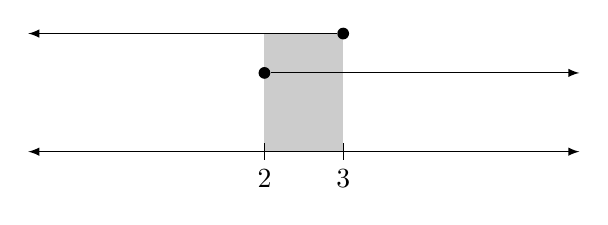
\begin{tikzpicture}
              \fill[black!20](2,0)rectangle(3,1.5);
              \draw[latex-latex] (-1,0) -- (6,0);
              \foreach \x in {2, 3} \draw[shift={(\x,0)},color=black] (0pt,3pt) -- (0pt,-3pt) node[below] {$\x$};
              \node[circle,fill,inner sep=1.5pt](a)at(2,1){};
              \node[circle,fill,inner sep=1.5pt](b)at(3,1.5){};
              \draw[-latex,black](a)--(6,1);
              \draw[-latex,black](b)--(-1,1.5);
            \end{tikzpicture}
          \end{center}

          \setcounter{equation}{0}
    \item \begin{numcases}{}
            3x + 4 > 1\\
            3x -1 \leq{} 2x + 2\\
            1 -2x > 5 -x
          \end{numcases}
          \sol{}
          \begin{flalign*}
            (1): 3x      & > -3               \\
            x            & > -1               \\
            (2): x       & \leq{} 3           \\
            (3): -x      & > 4                \\
            x            & < -4               \\
            \\
            \therefore\  & \text{No solution}
          \end{flalign*}
          \begin{center}
            \begin{tikzpicture}
              \draw[latex-latex] (-5,0) -- (2,0);
              \draw[shift={(-4,0)},color=black] (0pt,3pt) -- (0pt,-3pt) node[below] {-4};
              \draw[shift={(-2,0)},color=black] (0pt,3pt) -- (0pt,-3pt) node[below] {-1};
              \draw[shift={(1,0)},color=black] (0pt,3pt) -- (0pt,-3pt) node[below] {3};
              \node[circle,fill,inner sep=1.5pt](c)at(-4,1){};
              \node[circle,fill,inner sep=1.5pt](a)at(1,1.5){};
              \node[circle,draw,fill=white,inner sep=1.5pt](b)at(-2,2){};
              \draw[-latex,black](a)--(-5,1.5);
              \draw[-latex,black](b)--(2,2);
              \draw[-latex,black](c)--(-5,1);
            \end{tikzpicture}
          \end{center}

          \setcounter{equation}{0}
    \item \begin{numcases}{}
            2x -\frac{1}{3} < 3 -\frac{x}{2}\\
            2(1-x) \leq{} \frac{4x}{3}\\
            4(3x-1) > 1 + \frac{9x}{2}
          \end{numcases}
          \sol{}
          \begin{flalign*}
            (1): 12 -2               & < 18 -3x            \\
            15x                      & < 20                \\
            x                        & < \frac{4}{3}       \\
            (2): 2 -2x               & \leq{} \frac{4x}{3} \\
            6 - 6x                   & \leq{} 4x           \\
            -10x                     & \leq{} -6           \\
            x                        & \geq{} \frac{3}{5}  \\
            (3): 12x - 4             & > 1 + \frac{9x}{2}  \\
            24x - 8                  & > 2 + 9x            \\
            15x                      & > 10                \\
            x                        & > \frac{2}{3}       \\
            \\
            \therefore\  \frac{2}{3} & < x < \frac{4}{3}
          \end{flalign*}
          \begin{center}
            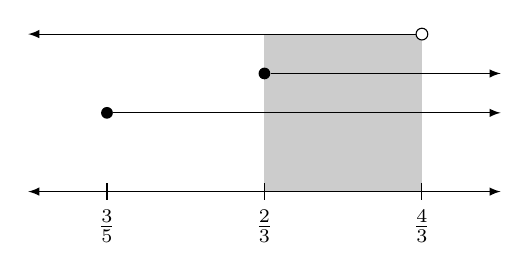
\begin{tikzpicture}
              \fill[black!20](3,0)rectangle(5,2);
              \draw[latex-latex] (0,0) -- (6,0);
              \draw[shift={(1,0)},color=black] (0pt,3pt) -- (0pt,-3pt) node[below] {$\frac{3}{5}$};
              \draw[shift={(3,0)},color=black] (0pt,3pt) -- (0pt,-3pt) node[below] {$\frac{2}{3}$};
              \draw[shift={(5,0)},color=black] (0pt,3pt) -- (0pt,-3pt) node[below] {$\frac{4}{3}$};
              \node[circle,fill,inner sep=1.5pt](c)at(1,1){};
              \node[circle,fill,inner sep=1.5pt](a)at(3,1.5){};
              \node[circle,draw,fill=white,inner sep=1.5pt](b)at(5,2){};
              \draw[-latex,black](c)--(6,1);
              \draw[-latex,black](a)--(6,1.5);
              \draw[-latex,black](b)--(0,2);
            \end{tikzpicture}
          \end{center}

    \item $-4 + x \leq{} 6 - x \leq{} 10$
          \sol{}
          \setcounter{equation}{0}
          \begin{numcases}{}
            -4 + x \leq{} 6 -x\\
            6 -x \leq{} 10
          \end{numcases}
          \begin{flalign*}
            (1): 2x       & \leq{} 10         \\
            x             & \leq{} 5          \\
            (2): -x       & \leq{} 4          \\
            x             & \geq{} 4          \\
            \\
            \therefore\ 4 & \leq{} x \leq{} 5
          \end{flalign*}

    \item $x - 2 \leq 2x + 5 < 3$
          \sol{}
          \setcounter{equation}{0}
          \begin{numcases}{}
            x -2 \leq{} 2x + 5\\
            2x + 5 < 3
          \end{numcases}
          \begin{flalign*}
            (1): -x        & \leq 7      \\
            x              & \geq -7     \\
            (2): 2x        & < -2        \\
            x              & < -1        \\
            \\
            \therefore\ -7 & \leq x < -1
          \end{flalign*}
          \begin{center}
            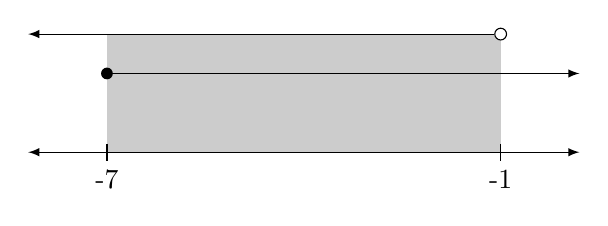
\begin{tikzpicture}
              \fill[black!20](-7,0)rectangle(-2,1.5);
              \draw[latex-latex] (-8,0) -- (-1,0);
              \draw[shift={(-7,0)},color=black] (0pt,3pt) -- (0pt,-3pt) node[below] {-7};
              \draw[shift={(-2,0)},color=black] (0pt,3pt) -- (0pt,-3pt) node[below] {-1};
              \node[circle,fill,inner sep=1.5pt](a)at(-7,1){};
              \node[circle,draw,fill=white,inner sep=1.5pt](b)at(-2,1.5){};
              \draw[-latex,black](a)--(-1,1);
              \draw[-latex,black](b)--(-8,1.5);
            \end{tikzpicture}
          \end{center}

  \end{enumerate}

  \section{Quadratic Inequalities}

  \subsection*{Solution of Quadratic Inequalities}

  The inequalities containing only one variable, and the highest exponent of the
  variable is 2, are called quadratic inequalities.

  We can solve the quadratic inequalities by first arraging the terms in the form
  of $ax^2+bx+c > 0$ or $ax^2+bx+c < 0$, where $a > 0$, then solve the quadratic
  equation $ax^2+bx+c = 0$, and finally, compare the solutions with the
  inequality sign.

  Note that for all real numbers, thier square is always positive.

  \subsection{Practice 5}

  Solve the following inequalities:

  \begin{enumerate}

    \item $x^2 + 3x \leq 54$
          \sol{}
          \begin{flalign*}
            x^2 + 3x       & \leq 54              \\
            x^2 + 3x - 54  & \leq 0               \\
            (x - 6)(x + 9) & \leq 0               \\
            x \leq -9      & \text{ or } x \geq 6
          \end{flalign*}
          \begin{center}
            \begin{tikzpicture}
              \draw[latex-latex] (0,0) -- (6,0);
              \draw[shift={(2,0)},color=black] (0pt,3pt) -- (0pt,-3pt) node[below] {$-9$};
              \draw[shift={(4,0)},color=black] (0pt,3pt) -- (0pt,-3pt) node[below] {6};
              \draw[shift={(3,0)},color=black] node[above] {$-$};
              \draw[shift={(1,0)},color=black] node[above] {$+$};
              \draw[shift={(5,0)},color=black] node[above] {$+$};
              \node[circle,fill,inner sep=1.5pt](a)at(4,1){};
              \node[circle,fill,inner sep=1.5pt](b)at(2,1){};
              \draw[-latex,black](a)--(6,1);
              \draw[-latex,black](b)--(0,1);
            \end{tikzpicture}
          \end{center}

    \item $4x^2 > 1$
          \sol{}
          \begin{flalign*}
            4x^2             & > 1                         \\
            4x^2 - 1         & > 0                         \\
            (2x - 1)(2x + 1) & > 0                         \\
            x < -\frac{1}{2} & \text{ or } x > \frac{1}{2}
          \end{flalign*}
          \begin{center}
            \begin{tikzpicture}
              \draw[latex-latex] (0,0) -- (6,0);
              \draw[shift={(2,0)},color=black] (0pt,3pt) -- (0pt,-3pt) node[below] {$-\frac{1}{2}$};
              \draw[shift={(4,0)},color=black] (0pt,3pt) -- (0pt,-3pt) node[below] {$\frac{1}{2}$};
              \draw[shift={(1,0)},color=black] node[above] {$+$};
              \draw[shift={(3,0)},color=black] node[above] {$-$};
              \draw[shift={(5,0)},color=black] node[above] {$+$};
              \node[circle,draw,fill=white,inner sep=1.5pt](a)at(2,1){};
              \node[circle,draw,fill=white,inner sep=1.5pt](b)at(4,1){};
              \draw[-latex,black](a)--(0,1);
              \draw[-latex,black](b)--(6,1);
            \end{tikzpicture}
          \end{center}

    \item $3 + 2x - x^2 \geq 0$
          \sol{}
          \begin{flalign*}
            3 + 2x - x^2   & \geq 0 \\
            -x^2 + 2x + 3  & \geq 0 \\
            x^2 - 2x - 3   & \leq 0 \\
            (x - 3)(x + 1) & \leq 0 \\
            -1 \leq x      & \leq 3
          \end{flalign*}
          \begin{center}
            \begin{tikzpicture}
              \draw[latex-latex] (0,0) -- (6,0);
              \draw[shift={(2,0)},color=black] (0pt,3pt) -- (0pt,-3pt) node[below] {$-1$};
              \draw[shift={(4,0)},color=black] (0pt,3pt) -- (0pt,-3pt) node[below] {3};
              \draw[shift={(1,0)},color=black] node[above] {$+$};
              \draw[shift={(3,0)},color=black] node[above] {$-$};
              \draw[shift={(5,0)},color=black] node[above] {$+$};
              \node[circle,fill,inner sep=1.5pt](a)at(2,1){};
              \draw (a)--(4,1);
              \node[circle,fill,inner sep=1.5pt](b)at(4,1){};
            \end{tikzpicture}
          \end{center}

    \item $2x^2 < 3x$
          \sol{}
          \begin{flalign*}
            2x^2 - 3x & < 0           \\
            x(2x - 3) & < 0           \\
            0 < x     & < \frac{3}{2}
          \end{flalign*}
          \begin{center}
            \begin{tikzpicture}
              \draw[latex-latex] (0,0) -- (6,0);
              \draw[shift={(2,0)},color=black] (0pt,3pt) -- (0pt,-3pt) node[below] {0};
              \draw[shift={(4,0)},color=black] (0pt,3pt) -- (0pt,-3pt) node[below] {$\frac{3}{2}$};
              \draw[shift={(1,0)},color=black] node[above] {$+$};
              \draw[shift={(3,0)},color=black] node[above] {$-$};
              \draw[shift={(5,0)},color=black] node[above] {$+$};
              \node[circle,draw,fill=white,inner sep=1.5pt](a)at(2,1){};
              \draw (a)--(4,1);
              \node[circle,draw,fill=white,inner sep=1.5pt](b)at(4,1){};
            \end{tikzpicture}
          \end{center}

  \end{enumerate}

  \subsection{Exercise 15.3a}

  Solve the following inequalities:

  \begin{enumerate}

    \item $x^4 + 4x + 3 > 0$
          \sol{}
          \begin{flalign*}
            x^2 + 4x + 3 & > 0                \\
            (x+3)(x+1)   & > 0                \\
            x < -3       & \text{ or } x > -1
          \end{flalign*}
          \begin{center}
            \begin{tikzpicture}
              \draw[latex-latex] (0,0) -- (6,0);
              \draw[shift={(2,0)},color=black] (0pt,3pt) -- (0pt,-3pt) node[below] {$-3$};
              \draw[shift={(4,0)},color=black] (0pt,3pt) -- (0pt,-3pt) node[below] {$-1$};
              \draw[shift={(1,0)},color=black] node[above] {$+$};
              \draw[shift={(3,0)},color=black] node[above] {$-$};
              \draw[shift={(5,0)},color=black] node[above] {$+$};
              \node[circle,draw,fill=white,inner sep=1.5pt](a)at(2,1){};
              \node[circle,draw,fill=white,inner sep=1.5pt](b)at(4,1){};
              \draw[-latex,black](a)--(0,1);
              \draw[-latex,black](b)--(6,1);
            \end{tikzpicture}
          \end{center}

    \item $x^2 + 2x - 8 \leq 0$
          \sol{}
          \begin{flalign*}
            x^2 + 2x - 8 & \leq 0 \\
            (x+4)(x-2)   & \leq 0 \\
            -4 \leq x    & \leq 2
          \end{flalign*}
          \begin{center}
            \begin{tikzpicture}
              \draw[latex-latex] (0,0) -- (6,0);
              \draw[shift={(2,0)},color=black] (0pt,3pt) -- (0pt,-3pt) node[below] {$-4$};
              \draw[shift={(4,0)},color=black] (0pt,3pt) -- (0pt,-3pt) node[below] {2};
              \draw[shift={(1,0)},color=black] node[above] {$+$};
              \draw[shift={(3,0)},color=black] node[above] {$-$};
              \draw[shift={(5,0)},color=black] node[above] {$+$};
              \node[circle,fill,inner sep=1.5pt](a)at(2,1){};
              \draw (a)--(4,1);
              \node[circle,fill,inner sep=1.5pt](b)at(4,1){};
            \end{tikzpicture}
          \end{center}

    \item $4x + 12 > x^2$
          \sol{}
          \begin{flalign*}
            4x + 12       & > x^2 \\
            x^2 - 4x - 12 & < 0   \\
            (x-6)(x+2)    & < 0   \\
            -2 < x        & < 6
          \end{flalign*}
          \begin{center}
            \begin{tikzpicture}
              \draw[latex-latex] (0,0) -- (6,0);
              \draw[shift={(2,0)},color=black] (0pt,3pt) -- (0pt,-3pt) node[below] {$-2$};
              \draw[shift={(4,0)},color=black] (0pt,3pt) -- (0pt,-3pt) node[below] {6};
              \draw[shift={(1,0)},color=black] node[above] {$+$};
              \draw[shift={(3,0)},color=black] node[above] {$-$};
              \draw[shift={(5,0)},color=black] node[above] {$+$};
              \node[circle,draw,fill=white,inner sep=1.5pt](a)at(2,1){};
              \draw (a)--(4,1);
              \node[circle,draw,fill=white,inner sep=1.5pt](b)at(4,1){};
            \end{tikzpicture}
          \end{center}

    \item $9x^2 \geq 16$
          \sol{}
          \begin{flalign*}
            9x^2 - 16           & \geq 0                         \\
            (3x+4)(3x-4)        & \geq 0                         \\
            x \leq -\frac{4}{3} & \text{ or } x \geq \frac{4}{3}
          \end{flalign*}
          \begin{center}
            \begin{tikzpicture}
              \draw[latex-latex] (0,0) -- (6,0);
              \draw[shift={(2,0)},color=black] (0pt,3pt) -- (0pt,-3pt) node[below] {$-\frac{4}{3}$};
              \draw[shift={(4,0)},color=black] (0pt,3pt) -- (0pt,-3pt) node[below] {$\frac{4}{3}$};
              \draw[shift={(1,0)},color=black] node[above] {$+$};
              \draw[shift={(3,0)},color=black] node[above] {$-$};
              \draw[shift={(5,0)},color=black] node[above] {$+$};
              \node[circle,fill,inner sep=1.5pt](a)at(2,1){};
              \node[circle,fill,inner sep=1.5pt](b)at(4,1){};
              \draw[-latex,black](a)--(0,1);
              \draw[-latex,black](b)--(6,1);
            \end{tikzpicture}
          \end{center}

    \item $(x+2)(x-3) \leq 6$
          \sol{}
          \begin{flalign*}
            (x+2)(x-3)   & \leq 6 \\
            x^2 - x - 6  & \leq 6 \\
            x^2 - x - 12 & \leq 0 \\
            (x-4)(x+3)   & \leq 0 \\
            -3 \leq x    & \leq 4
          \end{flalign*}
          \begin{center}
            \begin{tikzpicture}
              \draw[latex-latex] (0,0) -- (6,0);
              \draw[shift={(2,0)},color=black] (0pt,3pt) -- (0pt,-3pt) node[below] {-3};
              \draw[shift={(4,0)},color=black] (0pt,3pt) -- (0pt,-3pt) node[below] {4};
              \draw[shift={(1,0)},color=black] node[above] {$+$};
              \draw[shift={(3,0)},color=black] node[above] {$-$};
              \draw[shift={(5,0)},color=black] node[above] {$+$};
              \node[circle,fill,inner sep=1.5pt](a)at(2,1){};
              \draw (a)--(4,1);
              \node[circle,fill,inner sep=1.5pt](b)at(4,1){};
            \end{tikzpicture}
          \end{center}

    \item $x(x+2) < x(3-x) + 1$
          \sol{}
          \begin{flalign*}
            x(x+2)       & < x(3-x) + 1   \\
            x^2 + 2x     & < 3x - x^2 + 1 \\
            2x^2 - x - 1 & < 0            \\
            (x-1)(2x+1)  & < 0            \\
            -\frac{1}{2} & < x < 1
          \end{flalign*}
          \begin{center}
            \begin{tikzpicture}
              \draw[latex-latex] (0,0) -- (6,0);
              \draw[shift={(2,0)},color=black] (0pt,3pt) -- (0pt,-3pt) node[below] {$-\frac{1}{2}$};
              \draw[shift={(4,0)},color=black] (0pt,3pt) -- (0pt,-3pt) node[below] {1};
              \draw[shift={(1,0)},color=black] node[above] {$+$};
              \draw[shift={(3,0)},color=black] node[above] {$-$};
              \draw[shift={(5,0)},color=black] node[above] {$+$};
              \node[circle,draw,fill=white,inner sep=1.5pt](a)at(2,1){};
              \draw (a)--(4,1);
              \node[circle,draw,fill=white,inner sep=1.5pt](b)at(4,1){};
            \end{tikzpicture}
          \end{center}

    \item $16x^2 - 3x + 1 \geq 5x$
          \sol{}
          \begin{flalign*}
            16x^2 - 3x + 1 & \geq 5x        \\
            16x^2 - 8x + 1 & \geq 0         \\
            {(4x - 1)}^2   & \geq 0         \\
            x              & \in \mathbb{R} \\
          \end{flalign*}

    \item ${(x-4)}^2 + {(x-6)}^2 \leq 2$
          \sol{}
          \begin{flalign*}
            {(x-4)}^2 + {(x-6)}^2                  & \leq 2 \\
            x^2 - 8x + 16         + x^2 - 12x + 36 & \leq 2 \\
            2x^2 - 20x + 52                        & \leq 2 \\
            x^2 - 10x + 26                         & \leq 1 \\
            x^2 - 10x + 25                         & \leq 0 \\
            {(x-5)}^2                              & \leq 0 \\
            x                                      & = 5
          \end{flalign*}

    \item $1 < 4x(1-x)$
          \sol{}
          \begin{flalign*}
            1                & < 4x(1-x)         \\
            4x - 4x^2    - 1 & > 0               \\
            4x^2 - 4x + 1    & < 0               \\
            {(2x - 1)}^2     & < 0               \\
            \text{No}        & \ \text{solution}
          \end{flalign*}

    \item $x^2 - 3x + 9 > 3x(3-x)$
          \sol{}
          \begin{flalign*}
            x^2 - 3x + 9      & > 3x(3-x)            \\
            x^2 - 3x + 9      & > 9x - 3x^2          \\
            4x^2 - 12x + 9    & > 0                  \\
            {(2x - 3)}^2      & > 0                  \\
            x \in \mathbb{R}, & \ x \neq \frac{3}{2}
          \end{flalign*}
  \end{enumerate}

  \subsection*{Solution of System of Quadratic Inequalities}

  To solve a system of quadratic inequalities, we need to solve each inequality
  separately and then find the intersection of the solutions.

  \subsection{Practice 6}

  Solve the following system of inequalities:

  \begin{enumerate}

    \setcounter{equation}{0}
    \item \begin{numcases}{}
            x + 1 < 0\\
            x^2 -x -6 > 0
          \end{numcases}
          \sol{}
          \begin{flalign*}
             & (1): x           < 1                                                                          \\
             & (2): (x-3)(x+2)  > 0                                                                          \\
             & \ \ \ \ \ \ \ \ \ \ \ \ x < -2           \text{ or } x > 3
             & 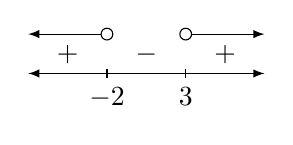
\begin{tikzpicture}[baseline={(current bounding box.center)},scale=0.5]
                 \draw[latex-latex] (0,0) -- (6,0);
                 \draw[shift={(2,0)},color=black] (0pt,3pt) -- (0pt,-3pt) node[below] {$-2$};
                 \draw[shift={(4,0)},color=black] (0pt,3pt) -- (0pt,-3pt) node[below] {3};
                 \draw[shift={(1,0)},color=black] node[above] {$+$};
                 \draw[shift={(3,0)},color=black] node[above] {$-$};
                 \draw[shift={(5,0)},color=black] node[above] {$+$};
                 \node[circle,draw,fill=white,inner sep=1.5pt](a)at(2,1){};
                 \node[circle,draw,fill=white,inner sep=1.5pt](b)at(4,1){};
                 \draw[-latex,black](a)--(0,1);
                 \draw[-latex,black](b)--(6,1);
               \end{tikzpicture} \\
             & \therefore\ x    < -2
          \end{flalign*}
          \begin{center}
            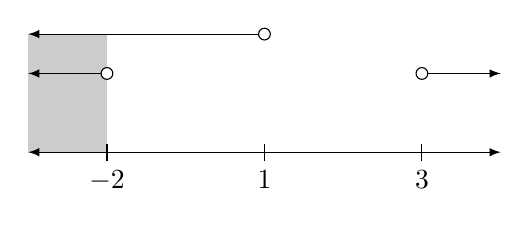
\begin{tikzpicture}
              \fill[black!20](0,0)rectangle(1,1.5);
              \draw[latex-latex] (0,0) -- (6,0);
              \draw[shift={(1,0)},color=black] (0pt,3pt) -- (0pt,-3pt) node[below] {$-2$};
              \draw[shift={(3,0)},color=black] (0pt,3pt) -- (0pt,-3pt) node[below] {1};
              \draw[shift={(5,0)},color=black] (0pt,3pt) -- (0pt,-3pt) node[below] {3};
              \node[circle,draw,fill=white,inner sep=1.5pt](a)at(1,1){};
              \node[circle,draw,fill=white,inner sep=1.5pt](b)at(5,1){};
              \node[circle,draw,fill=white,inner sep=1.5pt](c)at(3,1.5){};
              \draw[-latex,black](a)--(0,1);
              \draw[-latex,black](c)--(0,1.5);
              \draw[-latex,black](b)--(6,1);
            \end{tikzpicture}
          \end{center}

          \setcounter{equation}{0}
    \item \begin{numcases}{}
            x^2 -x -3 < 0\\
            x^2 + 3x -4 \leq 0
          \end{numcases}
          \sol{}
          \begin{flalign*}
             & (1): (x+1)(x-3)  < 0                                                                          \\
             & \ \ \ \ \ \ \ \ \ \ \ \ \ \ \ \ \ \ -1 < x < 3
             & 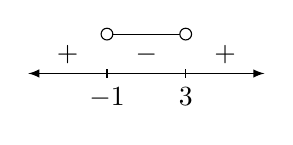
\begin{tikzpicture}[baseline={(current bounding box.center)},scale=0.5]
                 \draw[latex-latex] (0,0) -- (6,0);
                 \draw[shift={(2,0)},color=black] (0pt,3pt) -- (0pt,-3pt) node[below] {$-1$};
                 \draw[shift={(4,0)},color=black] (0pt,3pt) -- (0pt,-3pt) node[below] {3};
                 \draw[shift={(1,0)},color=black] node[above] {$+$};
                 \draw[shift={(3,0)},color=black] node[above] {$-$};
                 \draw[shift={(5,0)},color=black] node[above] {$+$};
                 \node[circle,draw,fill=white,inner sep=1.5pt](a)at(2,1){};
                 \draw(a)--(4,1);
                 \node[circle,draw,fill=white,inner sep=1.5pt](b)at(4,1){};
               \end{tikzpicture} \\
             & (2): (x+4)(x-1)  \leq 0                                                                       \\
             & \ \ \ \ \ \ \ \ \ \ \ \ \ \ \ \ \ \ -4 \leq x \leq 1
             & 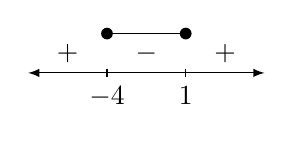
\begin{tikzpicture}[baseline={(current bounding box.center)},scale=0.5]
                 \draw[latex-latex] (0,0) -- (6,0);
                 \draw[shift={(2,0)},color=black] (0pt,3pt) -- (0pt,-3pt) node[below] {$-4$};
                 \draw[shift={(4,0)},color=black] (0pt,3pt) -- (0pt,-3pt) node[below] {1};
                 \draw[shift={(1,0)},color=black] node[above] {$+$};
                 \draw[shift={(3,0)},color=black] node[above] {$-$};
                 \draw[shift={(5,0)},color=black] node[above] {$+$};
                 \node[circle,fill,inner sep=1.5pt](a)at(2,1){};
                 \draw(a)--(4,1);
                 \node[circle,fill,inner sep=1.5pt](b)at(4,1){};
               \end{tikzpicture} \\
             & \therefore\ -1 < x \leq 1
          \end{flalign*}
          \begin{center}
            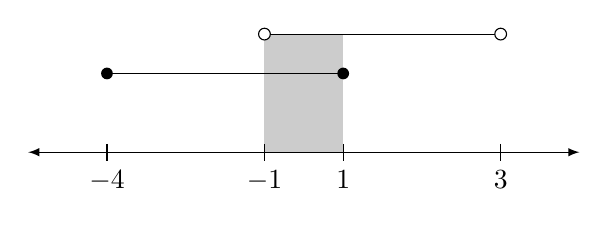
\begin{tikzpicture}
              \fill[black!20](3,0)rectangle(4,1.5);
              \draw[latex-latex] (0,0) -- (7,0);
              \draw[shift={(1,0)},color=black] (0pt,3pt) -- (0pt,-3pt) node[below] {$-4$};
              \draw[shift={(3,0)},color=black] (0pt,3pt) -- (0pt,-3pt) node[below] {$-1$};
              \draw[shift={(4,0)},color=black] (0pt,3pt) -- (0pt,-3pt) node[below] {1};
              \draw[shift={(6,0)},color=black] (0pt,3pt) -- (0pt,-3pt) node[below] {3};
              \node[circle,fill,inner sep=1.5pt](a)at(1,1){};
              \draw(a)--(4,1);
              \node[circle,fill,inner sep=1.5pt](b)at(4,1){};
              \node[circle,draw,fill=white,inner sep=1.5pt](c)at(3,1.5){};
              \draw(c)--(6,1.5);
              \node[circle,draw,fill=white,inner sep=1.5pt](d)at(6,1.5){};
            \end{tikzpicture}
          \end{center}

          \subsection{Exercise 15.3b}

          \setcounter{equation}{0}
    \item \begin{numcases}{}
            3x -4 \geq x -6\\
            x^2 -3x < 2x + 14
          \end{numcases}
          \sol{}
          \begin{flalign*}
             & (1): 2x \geq -2                                                                                \\
             & \ \ \ \ \ \ \ \ \ \ \ x \geq -1                                                                \\
             & (2): (x-7)(x+2) < 0                                                                            \\
             & \ \ \ \ \ \ \ \ \ \ \ \ \ \ \ \ \ \ -2 < x < 7
             & 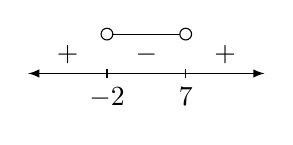
\begin{tikzpicture}[baseline={(current bounding box.center)},scale=0.5]
                 \draw[latex-latex] (0,0) -- (6,0);
                 \draw[shift={(2,0)},color=black] (0pt,3pt) -- (0pt,-3pt) node[below] {$-2$};
                 \draw[shift={(4,0)},color=black] (0pt,3pt) -- (0pt,-3pt) node[below] {$7$};
                 \draw[shift={(1,0)},color=black] node[above] {$+$};
                 \draw[shift={(3,0)},color=black] node[above] {$-$};
                 \draw[shift={(5,0)},color=black] node[above] {$+$};
                 \node[circle,draw,fill=white,inner sep=1.5pt](a)at(2,1){};
                 \draw(a)--(4,1);
                 \node[circle,draw,fill=white,inner sep=1.5pt](b)at(4,1){};
               \end{tikzpicture} \\
             & \therefore\ -1 \leq x < 7
          \end{flalign*}
          \begin{center}
            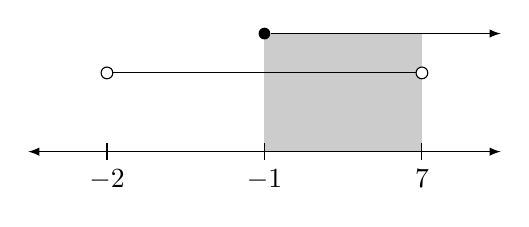
\begin{tikzpicture}
              \fill[black!20](3,0)rectangle(5,1.5);
              \draw[latex-latex] (0,0) -- (6,0);
              \draw[shift={(1,0)},color=black] (0pt,3pt) -- (0pt,-3pt) node[below] {$-2$};
              \draw[shift={(3,0)},color=black] (0pt,3pt) -- (0pt,-3pt) node[below] {$-1$};
              \draw[shift={(5,0)},color=black] (0pt,3pt) -- (0pt,-3pt) node[below] {$7$};
              \node[circle,draw,fill=white,inner sep=1.5pt](a)at(1,1){};
              \draw(a)--(5,1);
              \node[circle,draw,fill=white,inner sep=1.5pt](b)at(5,1){};
              \node[circle,fill,inner sep=1.5pt](c)at(3,1.5){};
              \draw[-latex,black](c)--(6,1.5);
            \end{tikzpicture}
          \end{center}

          \setcounter{equation}{0}
    \item \begin{numcases}{}
            x^2 + 5x + 4 > 0\\
            x^2 + 10x + 21 \geq 0
          \end{numcases}
          \sol{}
          \begin{flalign*}
             & (1): (x+4)(x+1) > 0                                                                            \\
             & \ \ \ \ \ \ \ \ \ \ \ \ x < -4 \text{ or } x > -1
             & 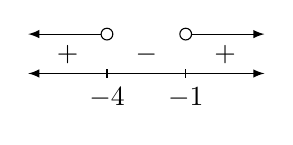
\begin{tikzpicture}[baseline={(current bounding box.center)},scale=0.5]
                 \draw[latex-latex] (0,0) -- (6,0);
                 \draw[shift={(2,0)},color=black] (0pt,3pt) -- (0pt,-3pt) node[below] {$-4$};
                 \draw[shift={(4,0)},color=black] (0pt,3pt) -- (0pt,-3pt) node[below] {$-1$};
                 \draw[shift={(1,0)},color=black] node[above] {$+$};
                 \draw[shift={(3,0)},color=black] node[above] {$-$};
                 \draw[shift={(5,0)},color=black] node[above] {$+$};
                 \node[circle,draw,fill=white,inner sep=1.5pt](a)at(2,1){};
                 \node[circle,draw,fill=white,inner sep=1.5pt](b)at(4,1){};
                 \draw[-latex,black](a)--(0,1);
                 \draw[-latex,black](b)--(6,1);
               \end{tikzpicture} \\
             & (2): (x+7)(x+3) \geq 0                                                                         \\
             & \ \ \ \ \ \ \ \ \ \ \ \ x \leq -7 \text{ or } x \geq -3
             & 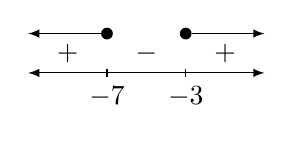
\begin{tikzpicture}[baseline={(current bounding box.center)},scale=0.5]
                 \draw[latex-latex] (0,0) -- (6,0);
                 \draw[shift={(2,0)},color=black] (0pt,3pt) -- (0pt,-3pt) node[below] {$-7$};
                 \draw[shift={(4,0)},color=black] (0pt,3pt) -- (0pt,-3pt) node[below] {$-3$};
                 \draw[shift={(1,0)},color=black] node[above] {$+$};
                 \draw[shift={(3,0)},color=black] node[above] {$-$};
                 \draw[shift={(5,0)},color=black] node[above] {$+$};
                 \node[circle,fill,inner sep=1.5pt](a)at(2,1){};
                 \node[circle,fill,inner sep=1.5pt](b)at(4,1){};
                 \draw[-latex,black](a)--(0,1);
                 \draw[-latex,black](b)--(6,1);
               \end{tikzpicture} \\
             & \therefore\ x \leq -7 \text{ or } x > -1
          \end{flalign*}
          \begin{center}
            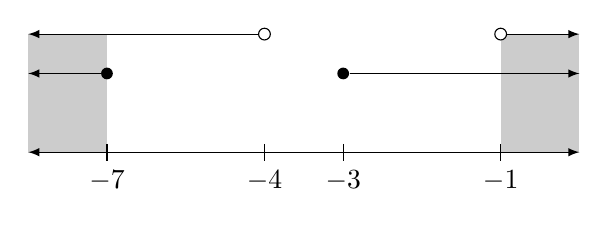
\begin{tikzpicture}
              \fill[black!20](0,0)rectangle(1,1.5);
              \fill[black!20](7,0)rectangle(6,1.5);
              \draw[latex-latex] (0,0) -- (7,0);
              \draw[shift={(1,0)},color=black] (0pt,3pt) -- (0pt,-3pt) node[below] {$-7$};
              \draw[shift={(3,0)},color=black] (0pt,3pt) -- (0pt,-3pt) node[below] {$-4$};
              \draw[shift={(4,0)},color=black] (0pt,3pt) -- (0pt,-3pt) node[below] {$-3$};
              \draw[shift={(6,0)},color=black] (0pt,3pt) -- (0pt,-3pt) node[below] {$-1$};
              \node[circle,fill,inner sep=1.5pt](a)at(1,1){};
              \node[circle,fill,inner sep=1.5pt](b)at(4,1){};
              \node[circle,draw,fill=white,inner sep=1.5pt](c)at(3,1.5){};
              \node[circle,draw,fill=white,inner sep=1.5pt](d)at(6,1.5){};
              \draw[-latex,black](a)--(0,1);
              \draw[-latex,black](b)--(7,1);
              \draw[-latex,black](c)--(0,1.5);
              \draw[-latex,black](d)--(7,1.5);
            \end{tikzpicture}
          \end{center}

          \setcounter{equation}{0}
    \item \begin{numcases}{}
            x^2 > 4\\
            4x (x-1) \leq 15
          \end{numcases}
          \sol{}
          \begin{flalign*}
             & \ \ \ (1): x^2 - 4 > 0                                                                                                \\
             & (x+2)(x-2) > 0                                                                                                        \\
             & \ \ \ \ x < -2 \text{ or } x > 2
             & 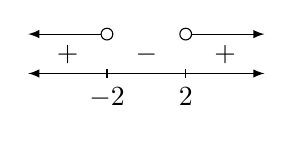
\begin{tikzpicture}[baseline={(current bounding box.center)},scale=0.5]
                 \draw[latex-latex] (0,0) -- (6,0);
                 \draw[shift={(2,0)},color=black] (0pt,3pt) -- (0pt,-3pt) node[below] {$-2$};
                 \draw[shift={(4,0)},color=black] (0pt,3pt) -- (0pt,-3pt) node[below] {$2$};
                 \draw[shift={(1,0)},color=black] node[above] {$+$};
                 \draw[shift={(3,0)},color=black] node[above] {$-$};
                 \draw[shift={(5,0)},color=black] node[above] {$+$};
                 \node[circle,draw,fill=white,inner sep=1.5pt](a)at(2,1){};
                 \node[circle,draw,fill=white,inner sep=1.5pt](b)at(4,1){};
                 \draw[-latex,black](a)--(0,1);
                 \draw[-latex,black](b)--(6,1);
               \end{tikzpicture}                        \\
             & (2): 4x^2 - 4x - 15 \leq 0                                                                                            \\
             & \ \ \ \ \ (2x + 3)(2x - 5) \leq 0                                                                                     \\
             & \ \ \ \ \ \ \ \ \ \ \ \ \ \ \ \ \ -\frac{3}{2} \leq x \leq \frac{5}{2}
             & 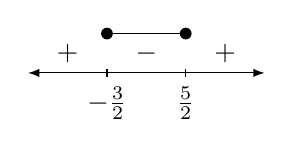
\begin{tikzpicture}[baseline={(current bounding box.center)},scale=0.5]
                 \draw[latex-latex] (0,0) -- (6,0);
                 \draw[shift={(2,0)},color=black] (0pt,3pt) -- (0pt,-3pt) node[below] {$-\frac{3}{2}$};
                 \draw[shift={(4,0)},color=black] (0pt,3pt) -- (0pt,-3pt) node[below] {$\frac{5}{2}$};
                 \draw[shift={(1,0)},color=black] node[above] {$+$};
                 \draw[shift={(3,0)},color=black] node[above] {$-$};
                 \draw[shift={(5,0)},color=black] node[above] {$+$};
                 \node[circle,fill,inner sep=1.5pt](a)at(2,1){};
                 \draw(a)--(4,1);
                 \node[circle,fill,inner sep=1.5pt](b)at(4,1){};
               \end{tikzpicture} \\
             & \therefore\ 2 < x \leq \frac{5}{2}
          \end{flalign*}
          \begin{center}
            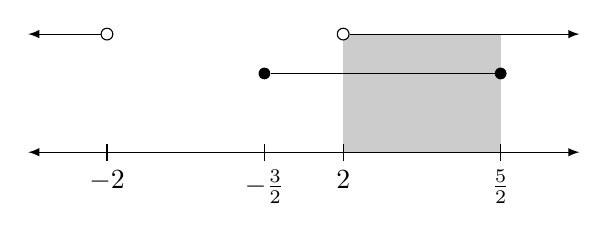
\begin{tikzpicture}
              \fill[black!20](4,0)rectangle(6,1.5);
              \draw[latex-latex] (0,0) -- (7,0);
              \draw[shift={(1,0)},color=black] (0pt,3pt) -- (0pt,-3pt) node[below] {$-2$};
              \draw[shift={(3,0)},color=black] (0pt,3pt) -- (0pt,-3pt) node[below] {$-\frac{3}{2}$};
              \draw[shift={(4,0)},color=black] (0pt,3pt) -- (0pt,-3pt) node[below] {$2$};
              \draw[shift={(6,0)},color=black] (0pt,3pt) -- (0pt,-3pt) node[below] {$\frac{5}{2}$};
              \node[circle,fill,inner sep=1.5pt](a)at(3,1){};
              \draw (a)--(6,1);
              \node[circle,fill,inner sep=1.5pt](b)at(6,1){};
              \node[circle,draw,fill=white,inner sep=1.5pt](c)at(1,1.5){};
              \node[circle,draw,fill=white,inner sep=1.5pt](d)at(4,1.5){};
              \draw[-latex,black](c)--(0,1.5);
              \draw[-latex,black](d)--(7,1.5);
            \end{tikzpicture}
          \end{center}

          \setcounter{equation}{0}
    \item \begin{numcases}{}
            x^2 + x < 6\\
            4(2x + 3) < (2-x)(1+x)
          \end{numcases}
          \sol{}
          \begin{flalign*}
             & (1): x^2 + x - 6 < 0                                                                           \\
             & \ \ \ (x+3)(x-2) < 0                                                                           \\
             & \ \ \ \ \ \ \ \ \ \ \ \ -3 < x < 2
             & 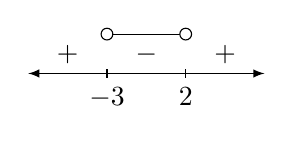
\begin{tikzpicture}[baseline={(current bounding box.center)},scale=0.5]
                 \draw[latex-latex] (0,0) -- (6,0);
                 \draw[shift={(2,0)},color=black] (0pt,3pt) -- (0pt,-3pt) node[below] {$-3$};
                 \draw[shift={(4,0)},color=black] (0pt,3pt) -- (0pt,-3pt) node[below] {$2$};
                 \draw[shift={(1,0)},color=black] node[above] {$+$};
                 \draw[shift={(3,0)},color=black] node[above] {$-$};
                 \draw[shift={(5,0)},color=black] node[above] {$+$};
                 \node[circle,draw,fill=white,inner sep=1.5pt](a)at(2,1){};
                 \draw(a)--(4,1);
                 \node[circle,draw,fill=white,inner sep=1.5pt](b)at(4,1){};
               \end{tikzpicture} \\
             & (2): 8x + 12 < 2 + x - x^2                                                                     \\
             & \ x^2 + 7x + 10 < 0                                                                            \\
             & (x+5)(x+2) < 0                                                                                 \\
             & \ \ \ \ \ \ \ \ \ \ -5 < x < -2
             & 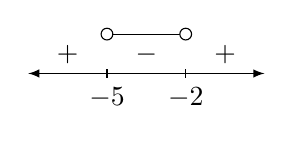
\begin{tikzpicture}[baseline={(current bounding box.center)},scale=0.5]
                 \draw[latex-latex] (0,0) -- (6,0);
                 \draw[shift={(2,0)},color=black] (0pt,3pt) -- (0pt,-3pt) node[below] {$-5$};
                 \draw[shift={(4,0)},color=black] (0pt,3pt) -- (0pt,-3pt) node[below] {$-2$};
                 \draw[shift={(1,0)},color=black] node[above] {$+$};
                 \draw[shift={(3,0)},color=black] node[above] {$-$};
                 \draw[shift={(5,0)},color=black] node[above] {$+$};
                 \node[circle,draw,fill=white,inner sep=1.5pt](a)at(2,1){};
                 \draw(a)--(4,1);
                 \node[circle,draw,fill=white,inner sep=1.5pt](b)at(4,1){};
               \end{tikzpicture} \\
             & \therefore\ -3 < x < -2
          \end{flalign*}
          \begin{center}
            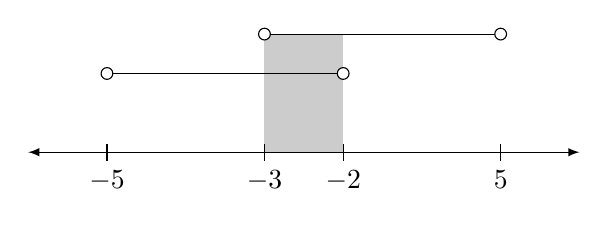
\begin{tikzpicture}
              \fill[black!20](3,0)rectangle(4,1.5);
              \draw[latex-latex] (0,0) -- (7,0);
              \draw[shift={(1,0)},color=black] (0pt,3pt) -- (0pt,-3pt) node[below] {$-5$};
              \draw[shift={(3,0)},color=black] (0pt,3pt) -- (0pt,-3pt) node[below] {$-3$};
              \draw[shift={(4,0)},color=black] (0pt,3pt) -- (0pt,-3pt) node[below] {$-2$};
              \draw[shift={(6,0)},color=black] (0pt,3pt) -- (0pt,-3pt) node[below] {5};
              \node[circle,draw,fill=white,inner sep=1.5pt](a)at(1,1){};
              \draw(a)--(4,1);
              \node[circle,draw,fill=white,inner sep=1.5pt](b)at(4,1){};
              \node[circle,draw,fill=white,inner sep=1.5pt](c)at(3,1.5){};
              \draw(c)--(6,1.5);
              \node[circle,draw,fill=white,inner sep=1.5pt](d)at(6,1.5){};
            \end{tikzpicture}
          \end{center}

          \setcounter{equation}{0}
    \item \begin{numcases}{}
            (x-1)(x+1) > 11 + 4x\\
            x^2 + 4 \leq 7x -2
          \end{numcases}
          \sol{}
          \begin{flalign*}
             & \ \ \ (1): x^2 - 1 > 11 + 4x                                                                   \\
             & \ x^2 - 4x - 12 > 0                                                                            \\
             & (x-6)(x+2) > 0                                                                                 \\
             & \ \ \ \ x < -2 \text{ or } x > 6
             & 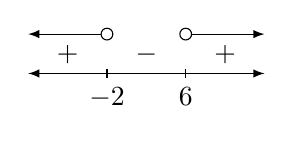
\begin{tikzpicture}[baseline={(current bounding box.center)},scale=0.5]
                 \draw[latex-latex] (0,0) -- (6,0);
                 \draw[shift={(2,0)},color=black] (0pt,3pt) -- (0pt,-3pt) node[below] {$-2$};
                 \draw[shift={(4,0)},color=black] (0pt,3pt) -- (0pt,-3pt) node[below] {$6$};
                 \draw[shift={(1,0)},color=black] node[above] {$+$};
                 \draw[shift={(3,0)},color=black] node[above] {$-$};
                 \draw[shift={(5,0)},color=black] node[above] {$+$};
                 \node[circle,draw,fill=white,inner sep=1.5pt](a)at(2,1){};
                 \node[circle,draw,fill=white,inner sep=1.5pt](b)at(4,1){};
                 \draw[-latex,black](a)--(0,1);
                 \draw[-latex,black](b)--(6,1);
               \end{tikzpicture} \\
             & (2): x^2 - 7x + 6 \leq 0                                                                       \\
             & \ \ \ \ \ \ (x-6)(x-1) \leq 0                                                                  \\
             & \ \ \ \ \ \ \ \ \ \ \ \ \ \ \ \ \ \ \ \ 1 \leq x \leq 6
             & 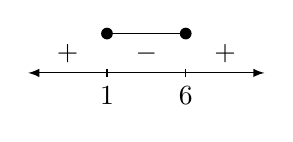
\begin{tikzpicture}[baseline={(current bounding box.center)},scale=0.5]
                 \draw[latex-latex] (0,0) -- (6,0);
                 \draw[shift={(2,0)},color=black] (0pt,3pt) -- (0pt,-3pt) node[below] {$1$};
                 \draw[shift={(4,0)},color=black] (0pt,3pt) -- (0pt,-3pt) node[below] {$6$};
                 \draw[shift={(1,0)},color=black] node[above] {$+$};
                 \draw[shift={(3,0)},color=black] node[above] {$-$};
                 \draw[shift={(5,0)},color=black] node[above] {$+$};
                 \node[circle,fill,inner sep=1.5pt](a)at(2,1){};
                 \draw(a)--(4,1);
                 \node[circle,fill,inner sep=1.5pt](b)at(4,1){};
               \end{tikzpicture}  \\
             & \therefore\ \text{No solution}
          \end{flalign*}
          \begin{center}
            \begin{tikzpicture}
              \draw[latex-latex] (0,0) -- (6,0);
              \draw[shift={(1,0)},color=black] (0pt,3pt) -- (0pt,-3pt) node[below] {$-2$};
              \draw[shift={(3,0)},color=black] (0pt,3pt) -- (0pt,-3pt) node[below] {$1$};
              \draw[shift={(5,0)},color=black] (0pt,3pt) -- (0pt,-3pt) node[below] {$6$};
              \node[circle,draw,fill=white,inner sep=1.5pt](a)at(1,1){};
              \node[circle,draw,fill=white,inner sep=1.5pt](b)at(5,1){};
              \node[circle,fill,inner sep=1.5pt](c)at(3,1.5){};
              \draw(c)--(5,1.5);
              \node[circle,fill,inner sep=1.5pt](c)at(5,1.5){};
              \draw[-latex,black](a)--(0,1);
              \draw[-latex,black](b)--(6,1);
            \end{tikzpicture}
          \end{center}

          \setcounter{equation}{0}
    \item \begin{numcases}{}
            x^2 -3x + 2 > 0\\
            x^2 + 3x \geq 0
          \end{numcases}
          \sol{}
          \begin{flalign*}
             & (1): (x-2)(x-1) > 0                                                                           \\
             & \ \ \ \ \ \ \ \ \ \ \ \ \ \ \ x < 1 \text{ or } x > 2
             & 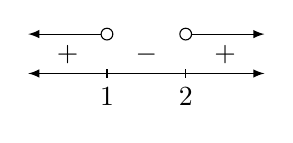
\begin{tikzpicture}[baseline={(current bounding box.center)},scale=0.5]
                 \draw[latex-latex] (0,0) -- (6,0);
                 \draw[shift={(2,0)},color=black] (0pt,3pt) -- (0pt,-3pt) node[below] {$1$};
                 \draw[shift={(4,0)},color=black] (0pt,3pt) -- (0pt,-3pt) node[below] {$2$};
                 \draw[shift={(1,0)},color=black] node[above] {$+$};
                 \draw[shift={(3,0)},color=black] node[above] {$-$};
                 \draw[shift={(5,0)},color=black] node[above] {$+$};
                 \node[circle,draw,fill=white,inner sep=1.5pt](a)at(2,1){};
                 \node[circle,draw,fill=white,inner sep=1.5pt](b)at(4,1){};
                 \draw[-latex,black](a)--(0,1);
                 \draw[-latex,black](b)--(6,1);
               \end{tikzpicture} \\
             & (2):  x(x+3) \geq 0                                                                           \\
             & \ \ \ x \leq -3 \text{ or } x \geq 0
             & 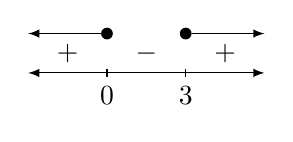
\begin{tikzpicture}[baseline={(current bounding box.center)},scale=0.5]
                 \draw[latex-latex] (0,0) -- (6,0);
                 \draw[shift={(2,0)},color=black] (0pt,3pt) -- (0pt,-3pt) node[below] {$0$};
                 \draw[shift={(4,0)},color=black] (0pt,3pt) -- (0pt,-3pt) node[below] {$3$};
                 \draw[shift={(1,0)},color=black] node[above] {$+$};
                 \draw[shift={(3,0)},color=black] node[above] {$-$};
                 \draw[shift={(5,0)},color=black] node[above] {$+$};
                 \node[circle,fill,inner sep=1.5pt](a)at(2,1){};
                 \node[circle,fill,inner sep=1.5pt](b)at(4,1){};
                 \draw[-latex,black](a)--(0,1);
                 \draw[-latex,black](b)--(6,1);
               \end{tikzpicture} \\
             & \therefore\ x < -3,\ 0 \leq x < 1,\ x > 2
          \end{flalign*}
          \begin{center}
            \begin{tikzpicture}
              \fill[black!20](0,0)rectangle(1,1.5);
              \fill[black!20](4,0)rectangle(3,1.5);
              \fill[black!20](7,0)rectangle(6,1.5);
              \draw[latex-latex] (0,0) -- (7,0);
              \draw[shift={(1,0)},color=black] (0pt,3pt) -- (0pt,-3pt) node[below] {$-3$};
              \draw[shift={(3,0)},color=black] (0pt,3pt) -- (0pt,-3pt) node[below] {$0$};
              \draw[shift={(4,0)},color=black] (0pt,3pt) -- (0pt,-3pt) node[below] {$1$};
              \draw[shift={(6,0)},color=black] (0pt,3pt) -- (0pt,-3pt) node[below] {$2$};
              \node[circle,fill,inner sep=1.5pt](a)at(1,1){};
              \node[circle,fill,inner sep=1.5pt](b)at(3,1){};
              \node[circle,draw,fill=white,inner sep=1.5pt](c)at(4,1.5){};
              \node[circle,draw,fill=white,inner sep=1.5pt](d)at(6,1.5){};
              \draw[-latex,black](a)--(0,1);
              \draw[-latex,black](b)--(7,1);
              \draw[-latex,black](c)--(0,1.5);
              \draw[-latex,black](d)--(7,1.5);
            \end{tikzpicture}
          \end{center}

          \setcounter{equation}{0}
    \item \begin{numcases}{}
            (x-3)(x+3) \geq 16\\
            x^2 + 3 \geq 13(x-3)
          \end{numcases}
          \sol{}
          \begin{flalign*}
             & \ \ \ \ \ \ \ \ \ \ \ \ x^2 - 9 \geq 16                                                        \\
             & \ \ \ \ \ \ \ \ \ \ x^2 - 25 \geq 0                                                            \\
             & (x+5)(x-5) \geq 0                                                                              \\
             & \ \ \ x \leq -5 \text{ or } x \geq 5
             & \begin{tikzpicture}[baseline={(current bounding box.center)},scale=0.5]
                 \draw[latex-latex] (0,0) -- (6,0);
                 \draw[shift={(2,0)},color=black] (0pt,3pt) -- (0pt,-3pt) node[below] {$-5$};
                 \draw[shift={(4,0)},color=black] (0pt,3pt) -- (0pt,-3pt) node[below] {$5$};
                 \draw[shift={(1,0)},color=black] node[above] {$+$};
                 \draw[shift={(3,0)},color=black] node[above] {$-$};
                 \draw[shift={(5,0)},color=black] node[above] {$+$};
                 \node[circle,fill,inner sep=1.5pt](a)at(2,1){};
                 \node[circle,fill,inner sep=1.5pt](b)at(4,1){};
                 \draw[-latex,black](a)--(0,1);
                 \draw[-latex,black](b)--(6,1);
               \end{tikzpicture} \\
             & (2): x^2 + 3 \geq 13x - 39                                                                     \\
             & x^2 - 13x + 42 \geq 0                                                                          \\
             & (x-7)(x-6) \geq 0                                                                              \\
             & \ \ \ \ \ \ x \leq 6 \text{ or } x \geq 7
             & \begin{tikzpicture}[baseline={(current bounding box.center)},scale=0.5]
                 \draw[latex-latex] (0,0) -- (6,0);
                 \draw[shift={(2,0)},color=black] (0pt,3pt) -- (0pt,-3pt) node[below] {$6$};
                 \draw[shift={(4,0)},color=black] (0pt,3pt) -- (0pt,-3pt) node[below] {$7$};
                 \draw[shift={(1,0)},color=black] node[above] {$+$};
                 \draw[shift={(3,0)},color=black] node[above] {$-$};
                 \draw[shift={(5,0)},color=black] node[above] {$+$};
                 \node[circle,fill,inner sep=1.5pt](a)at(2,1){};
                 \node[circle,fill,inner sep=1.5pt](b)at(4,1){};
                 \draw[-latex,black](a)--(0,1);
                 \draw[-latex,black](b)--(6,1);
               \end{tikzpicture}  \\
             & \therefore\ x \leq 5,\ 5 \leq x \leq 6,\ x \geq 7
          \end{flalign*}
          \begin{center}
            \begin{tikzpicture}
              \fill[black!20](0,0)rectangle(1,1.5);
              \fill[black!20](4,0)rectangle(3,1.5);
              \fill[black!20](7,0)rectangle(6,1.5);
              \draw[latex-latex] (0,0) -- (7,0);
              \draw[shift={(1,0)},color=black] (0pt,3pt) -- (0pt,-3pt) node[below] {$-5$};
              \draw[shift={(3,0)},color=black] (0pt,3pt) -- (0pt,-3pt) node[below] {$5$};
              \draw[shift={(4,0)},color=black] (0pt,3pt) -- (0pt,-3pt) node[below] {$6$};
              \draw[shift={(6,0)},color=black] (0pt,3pt) -- (0pt,-3pt) node[below] {$7$};
              \node[circle,fill,inner sep=1.5pt](a)at(1,1){};
              \node[circle,fill,inner sep=1.5pt](b)at(3,1){};
              \node[circle,fill,inner sep=1.5pt](c)at(4,1.5){};
              \node[circle,fill,inner sep=1.5pt](d)at(6,1.5){};
              \draw[-latex,black](a)--(0,1);
              \draw[-latex,black](b)--(7,1);
              \draw[-latex,black](c)--(0,1.5);
              \draw[-latex,black](d)--(7,1.5);
            \end{tikzpicture}
          \end{center}

          \setcounter{equation}{0}
    \item \begin{numcases}{}
            x^2 -x -1 \leq \frac{x-1}{6} \\
            (2x-1)(x-6) \geq 13
          \end{numcases}
          \sol{}
          \begin{flalign*}
             & (1): 6x^2 - 6x - 6 \leq x-1                                                                                           \\
             & \ \ \ \ \ \ \ \ \ 6x^2 -7x -5 \leq 0                                                                                  \\
             & \ \ \ (3x-5)(2x-1) \leq 0                                                                                             \\
             & \ \ \ \ \ \ \ \ \ \ \ \ \ \ \ -\frac{1}{2} \leq x \leq \frac{5}{3}
             & \begin{tikzpicture}[baseline={(current bounding box.center)},scale=0.5]
                 \draw[latex-latex] (0,0) -- (6,0);
                 \draw[shift={(2,0)},color=black] (0pt,3pt) -- (0pt,-3pt) node[below] {$-\frac{1}{2}$};
                 \draw[shift={(4,0)},color=black] (0pt,3pt) -- (0pt,-3pt) node[below] {$\frac{5}{3}$};
                 \draw[shift={(1,0)},color=black] node[above] {$+$};
                 \draw[shift={(3,0)},color=black] node[above] {$-$};
                 \draw[shift={(5,0)},color=black] node[above] {$+$};
                 \node[circle,fill,inner sep=1.5pt](a)at(2,1){};
                 \draw(a)--(4,1);
                 \node[circle,fill,inner sep=1.5pt](b)at(4,1){};
               \end{tikzpicture} \\
             & (2): 2x^2 - 13x + 6 \geq 13                                                                                           \\
             & \ \ \ \ \ \ \ \ \ 2x^2 - 13x - 7 \geq 0                                                                               \\
             & \ \ \ \ \ \ \ (2x+1)(x-7) \geq 0                                                                                      \\
             & \ \ \ \ \ \ \ \ \ \ \ \ \ \ x \leq -\frac{1}{2},\ x \geq 7                                                            \\
             & \therefore\ x = -\frac{1}{2}
          \end{flalign*}
          \begin{center}
            \begin{tikzpicture}
              \fill[black!20](0.9,0)rectangle(1.1,1.5);
              \draw[latex-latex] (0,0) -- (6,0);
              \draw[shift={(1,0)},color=black] (0pt,3pt) -- (0pt,-3pt) node[below] {$-\frac{1}{2}$};
              \draw[shift={(3,0)},color=black] (0pt,3pt) -- (0pt,-3pt) node[below] {$\frac{5}{3}$};
              \draw[shift={(5,0)},color=black] (0pt,3pt) -- (0pt,-3pt) node[below] {$7$};
              \node[circle,fill,inner sep=1.5pt](a)at(1,1){};
              \node[circle,fill,inner sep=1.5pt](b)at(5,1){};
              \node[circle,fill,inner sep=1.5pt](c)at(1,1.5){};
              \draw(c)--(3,1.5);
              \node[circle,fill,inner sep=1.5pt](c)at(3,1.5){};
              \draw[-latex,black](a)--(0,1);
              \draw[-latex,black](b)--(6,1);
            \end{tikzpicture}
          \end{center}
  \end{enumerate}

  \section{Solution of Linear Inequalities of Higher Degree}

  A linear inequality thay contains a variable raised to a power greater than 2
  is called a linear inequality of higher degree. To solve this type of
  inequality, we move all the terms with the variable to one side of the
  inequality, and make the coefficient of the polynomial to be positive.

  \subsection{Practice 7}

  Solve the following inequalities:

  \begin{enumerate}

    \item $x^3 - 7x - 6 \geq 0$
          \sol{}
          \begin{flalign*}
            x^3 - 7x - 6                    & \geq 0 \\
            (x+2)(x^2-2x-3)                 & \geq 0 \\
            (x+2)(x-3)(x+1)                 & \geq 0 \\
            -2 \leq x \leq -1 \text{ or } x & \geq 3
          \end{flalign*}
          \begin{center}
            \begin{tikzpicture}
              \draw[latex-latex] (0,0) -- (6,0);
              \draw[shift={(1,0)},color=black] (0pt,3pt) -- (0pt,-3pt) node[below] {$-2$};
              \draw[shift={(3,0)},color=black] (0pt,3pt) -- (0pt,-3pt) node[below] {$-1$};
              \draw[shift={(5,0)},color=black] (0pt,3pt) -- (0pt,-3pt) node[below] {$3$};
              \draw[shift={(0.5,0)},color=black] node[above] {$-$};
              \draw[shift={(2,0)},color=black] node[above] {$+$};
              \draw[shift={(4,0)},color=black] node[above] {$-$};
              \draw[shift={(5.5,0)},color=black] node[above] {$+$};
              \node[circle,fill,inner sep=1.5pt](a)at(1,1){};
              \draw (a)--(3,1);
              \node[circle,fill,inner sep=1.5pt](b)at(3,1){};
              \node[circle,fill,inner sep=1.5pt](c)at(5,1){};
              \draw[-latex,black] (c)--(6,1);
            \end{tikzpicture}
          \end{center}

    \item $3x^2 + 18x + 8 > 2x^3$
          \sol{}
          \begin{flalign*}
            3x^2 + 18x + 8 - 2x^3               & > 0 \\
            2x^3 - 3x^2 - 18x - 8               & < 0 \\
            (x+2)(2x^2 - 7x - 4)                & < 0 \\
            (x+2)(2x + 1)(x-4)                  & < 0 \\
            x < -2 \text{ or } -\frac{1}{2} < x & < 4
          \end{flalign*}
          \begin{center}
            \begin{tikzpicture}
              \draw[latex-latex] (0,0) -- (6,0);
              \draw[shift={(1,0)},color=black] (0pt,3pt) -- (0pt,-3pt) node[below] {$-2$};
              \draw[shift={(3,0)},color=black] (0pt,3pt) -- (0pt,-3pt) node[below] {$-\frac{1}{2}$};
              \draw[shift={(5,0)},color=black] (0pt,3pt) -- (0pt,-3pt) node[below] {$4$};
              \draw[shift={(0.5,0)},color=black] node[above] {$-$};
              \draw[shift={(2,0)},color=black] node[above] {$+$};
              \draw[shift={(4,0)},color=black] node[above] {$-$};
              \draw[shift={(5.5,0)},color=black] node[above] {$+$};
              \node[circle,draw,fill=white,inner sep=1.5pt](a)at(3,1){};
              \draw (a)--(5,1);
              \node[circle,draw,fill=white,inner sep=1.5pt](b)at(5,1){};
              \node[circle,draw,fill=white,inner sep=1.5pt](c)at(1,1){};
              \draw[-latex,black] (c)--(0,1);
            \end{tikzpicture}
          \end{center}

    \item $x^4 + x^3 \leq 3x^2 + x - 2$
          \sol{}
          \begin{flalign*}
            x^4 + x^3 - 3x^2 - x + 2             & \leq 0  \\
            (x+2)[x^2(x-1) - (x-1)]              & \leq 0  \\
            (x+2)(x+1){(x-1)}^2                  & \leq 0  \\
            \text{When } x \neq 1,\    {(x+1)}^2 & > 0     \\
            (x+2)(x+1)                           & \leq 0  \\
            -2 \leq x                            & \leq -1 \\
            \text{When } x = 1,\    {(x+1)}^2    & = 0     \\
            \therefore\ x \text{ is the solution}          \\
            \therefore\ -2 \leq x \leq -1
          \end{flalign*}
          \begin{center}
            \begin{tikzpicture}[baseline={(current bounding box.center)}]
              \draw[latex-latex] (0,0) -- (6,0);
              \draw[shift={(2,0)},color=black] (0pt,3pt) -- (0pt,-3pt) node[below] {$-3$};
              \draw[shift={(4,0)},color=black] (0pt,3pt) -- (0pt,-3pt) node[below] {$2$};
              \draw[shift={(1,0)},color=black] node[above] {$+$};
              \draw[shift={(3,0)},color=black] node[above] {$-$};
              \draw[shift={(5,0)},color=black] node[above] {$+$};
              \node[circle,fill,inner sep=1.5pt](a)at(2,1){};
              \draw(a)--(4,1);
              \node[circle,fill,inner sep=1.5pt](b)at(4,1){};
            \end{tikzpicture}
          \end{center}

    \item $x^4 - x^3 - 5x^2 - 3x > 0$
          \sol{}
          \begin{flalign*}
            x^4 - x^3 - 5x^2 - 3x                  & > 0     \\
            x(x+1)(x^2 - 2x - 3)                   & > 0     \\
            x(x-3){(x+1)}^2                        & > 0     \\
            \text{When } x \neq -1,\    {(x+1)}^2  & > 0     \\
            x(x-3)                                 & > 0     \\
            x < 0 \text{ or } x                    & > 3     \\
            \text{When } x = -1,\    {(x+1)}^2     & = 0     \\
            \therefore\ x \text{ is not the solution}        \\
            \therefore\ x < 0 \text{ or } x > 3, x & \neq -1
          \end{flalign*}
          \begin{center}
            \begin{tikzpicture}
              \draw[latex-latex] (0,0) -- (6,0);
              \draw[shift={(2,0)},color=black] (0pt,3pt) -- (0pt,-3pt) node[below] {$0$};
              \draw[shift={(4,0)},color=black] (0pt,3pt) -- (0pt,-3pt) node[below] {$3$};
              \draw[shift={(1,0)},color=black] node[above] {$+$};
              \draw[shift={(3,0)},color=black] node[above] {$-$};
              \draw[shift={(5,0)},color=black] node[above] {$+$};
              \node[circle,draw,fill=white,inner sep=1.5pt](a)at(2,1){};
              \node[circle,draw,fill=white,inner sep=1.5pt](b)at(4,1){};
              \draw[-latex,black](a)--(0,1);
              \draw[-latex,black](b)--(6,1);
            \end{tikzpicture}
          \end{center}
  \end{enumerate}

  \subsection{Exercise 15.4}

  Solve the following inequalities:

  \begin{enumerate}

    \item $(x-1)(x+1)(2x + 1) < 0$
          \sol{}
          \begin{flalign*}
            (x-1)(x+1)(2x + 1)                              & < 0 \\
            \therefore\ x < -1 \text{ or } -\frac{1}{2} < x & < 1
          \end{flalign*}
          \begin{center}
            \begin{tikzpicture}
              \draw[latex-latex] (0,0) -- (6,0);
              \draw[shift={(1,0)},color=black] (0pt,3pt) -- (0pt,-3pt) node[below] {$-1$};
              \draw[shift={(3,0)},color=black] (0pt,3pt) -- (0pt,-3pt) node[below] {$-\frac{1}{2}$};
              \draw[shift={(5,0)},color=black] (0pt,3pt) -- (0pt,-3pt) node[below] {$1$};
              \draw[shift={(0.5,0)},color=black] node[above] {$-$};
              \draw[shift={(2,0)},color=black] node[above] {$+$};
              \draw[shift={(4,0)},color=black] node[above] {$-$};
              \draw[shift={(5.5,0)},color=black] node[above] {$+$};
              \node[circle,draw,fill=white,inner sep=1.5pt](a)at(3,1){};
              \draw (a)--(5,1);
              \node[circle,draw,fill=white,inner sep=1.5pt](b)at(5,1){};
              \node[circle,draw,fill=white,inner sep=1.5pt](c)at(1,1){};
              \draw[-latex,black] (c)--(0,1);
            \end{tikzpicture}
          \end{center}

    \item $(3x+6)(x+3)(5-x) \leq 0$
          \sol{}
          \begin{flalign*}
            (3x+6)(x+3)(5-x)                            & \leq 0 \\
            -3(x+2)(x+3)(x-5)                           & \leq 0 \\
            (x+2)(x+3)(x-5)                             & \geq 0 \\
            \therefore\ -3 \leq x \leq -2 \text{ or } x & \geq 5
          \end{flalign*}
          \begin{center}
            \begin{tikzpicture}
              \draw[latex-latex] (0,0) -- (6,0);
              \draw[shift={(1,0)},color=black] (0pt,3pt) -- (0pt,-3pt) node[below] {$-3$};
              \draw[shift={(3,0)},color=black] (0pt,3pt) -- (0pt,-3pt) node[below] {$-2$};
              \draw[shift={(5,0)},color=black] (0pt,3pt) -- (0pt,-3pt) node[below] {$5$};
              \draw[shift={(0.5,0)},color=black] node[above] {$-$};
              \draw[shift={(2,0)},color=black] node[above] {$+$};
              \draw[shift={(4,0)},color=black] node[above] {$-$};
              \draw[shift={(5.5,0)},color=black] node[above] {$+$};
              \node[circle,fill,inner sep=1.5pt](a)at(1,1){};
              \draw (a)--(3,1);
              \node[circle,fill,inner sep=1.5pt](b)at(3,1){};
              \node[circle,fill,inner sep=1.5pt](c)at(5,1){};
              \draw[-latex,black] (c)--(6,1);
            \end{tikzpicture}
          \end{center}

    \item $4x^3 + 8x^2 - x - 2 \leq 0$
          \sol{}
          \begin{flalign*}
            4x^2(x + 2) - (x + 2)                                 & \leq 0           \\
            (4x^2 - 1)(x+2)                                       & \leq 0           \\
            (2x + 1)(2x - 1)(x + 2)                               & \leq 0           \\
            \therefore\ x \leq -2 \text{ or } -\frac{1}{2} \leq x & \leq \frac{1}{2}
          \end{flalign*}
          \begin{center}
            \begin{tikzpicture}
              \draw[latex-latex] (0,0) -- (6,0);
              \draw[shift={(1,0)},color=black] (0pt,3pt) -- (0pt,-3pt) node[below] {$-2$};
              \draw[shift={(3,0)},color=black] (0pt,3pt) -- (0pt,-3pt) node[below] {$-\frac{1}{2}$};
              \draw[shift={(5,0)},color=black] (0pt,3pt) -- (0pt,-3pt) node[below] {$\frac{1}{2}$};
              \draw[shift={(0.5,0)},color=black] node[above] {$-$};
              \draw[shift={(2,0)},color=black] node[above] {$+$};
              \draw[shift={(4,0)},color=black] node[above] {$-$};
              \draw[shift={(5.5,0)},color=black] node[above] {$+$};
              \node[circle,fill,inner sep=1.5pt](a)at(3,1){};
              \draw (a)--(5,1);
              \node[circle,fill,inner sep=1.5pt](b)at(5,1){};
              \node[circle,fill,inner sep=1.5pt](c)at(1,1){};
              \draw[-latex,black] (c)--(0,1);
            \end{tikzpicture}
          \end{center}

    \item $x^3 - 3x^2 + 3x - 1 \geq 0$
          \sol{}
          \begin{flalign*}
            x^3 - 3x^2 + 3x - 1        & \geq 0                          \\
            {(x-1)}^3                  & \geq 0                          \\
            (x-1){(x-1)}^2             & \geq 0                          \\
            \because\ {(x-1)}^2 \geq 0 & \text{ for all real numbers } x \\
            \therefore\ (x-1)          & \geq 0                          \\
            x                          & \geq 1
          \end{flalign*}
    \item $x^4 > 81$
          \sol{}
          \begin{flalign*}
            x^4                    & > 81                            \\
            x^4 - 81               & > 0                             \\
            (x^2 - 9)(x^2 + 9)     & > 0                             \\
            (x+3)(x-3)(x^2 + 9)    & > 0                             \\
            \because\ x^2 + 9 > 0  & \text{ for all real numbers } x \\
            \therefore\ (x+3)(x-3) & > 0                             \\
            x < -3 \text{ or } x   & > 3
          \end{flalign*}
          \begin{center}
            \begin{tikzpicture}
              \draw[latex-latex] (0,0) -- (6,0);
              \draw[shift={(2,0)},color=black] (0pt,3pt) -- (0pt,-3pt) node[below] {$-3$};
              \draw[shift={(4,0)},color=black] (0pt,3pt) -- (0pt,-3pt) node[below] {$3$};
              \draw[shift={(1,0)},color=black] node[above] {$+$};
              \draw[shift={(3,0)},color=black] node[above] {$-$};
              \draw[shift={(5,0)},color=black] node[above] {$+$};
              \node[circle,fill,inner sep=1.5pt](a)at(2,1){};
              \node[circle,fill,inner sep=1.5pt](b)at(4,1){};
              \draw[-latex,black](a)--(0,1);
              \draw[-latex,black](b)--(6,1);
            \end{tikzpicture}
          \end{center}

    \item $x^3{(x+2)}^2(x+3) > 0$
          \sol{}
          \begin{flalign*}
            x^3{(x+2)}^2(x+3)                                       & > 0              & \\
            x^2{(x+2)}^2[x(x+3)]                                    & > 0              & \\
            \text{For all real numbers }                            & x   \text{, }    & \\
            x^2 > 0 \text{ when } x                                 & \neq 0           & \\
            {(x+2)}^2 > 0 \text{ when } x                           & \neq -2          & \\
            x(x+3)                                                  & > 0              & \\
            \therefore\ x < -3 \text{ or } x                        & > 0              & \\
            \text{When } x = -2 \text{ or } x                       & = 0,             & \\
            x^3{(x+2)}^2(x+3)                                       & = 0              & \\
            \therefore\ x = 0 \text{ and } x = -2  \text{ are not } & \text{solution.} & \\
            \\
            \therefore\ x < -3 \text{ or } x                        & > 0,\ x \neq -2
          \end{flalign*}
          \begin{center}
            \begin{tikzpicture}
              \draw[latex-latex] (0,0) -- (6,0);
              \draw[shift={(2,0)},color=black] (0pt,3pt) -- (0pt,-3pt) node[below] {$-3$};
              \draw[shift={(4,0)},color=black] (0pt,3pt) -- (0pt,-3pt) node[below] {$0$};
              \draw[shift={(1,0)},color=black] node[above] {$+$};
              \draw[shift={(3,0)},color=black] node[above] {$-$};
              \draw[shift={(5,0)},color=black] node[above] {$+$};
              \node[circle,draw,fill=white,inner sep=1.5pt](a)at(2,1){};
              \node[circle,draw,fill=white,inner sep=1.5pt](b)at(4,1){};
              \draw[-latex,black](a)--(0,1);
              \draw[-latex,black](b)--(6,1);
            \end{tikzpicture}
          \end{center}

    \item ${(x-3)}^5{(x-1)}^3(x+2) < 0$
          \sol{}
          \begin{flalign*}
            {(x-3)}^4{(x-1)}^2[(x-3)(x-1)(x+2)]                   & < 0              &     \\
            \text{For all real numbers }                          & x \text{, }      &     \\
            {(x-3)}^4 > 0 \text{ when }                           & x \neq 3         &     \\
            {(x-1)}^2 > 0 \text{ when }                           & x \neq 1         &     \\
            (x-3)(x-1)(x+2)                                       & < 0              &     \\
            \therefore\ x < -2 \text{ or } 1 < x                  & < 3              &     \\
            \text{When } x = 3 \text{ or } x                      & = 1,             &     \\
            {(x-3)}^4{(x-1)}^2(x+2)                               & = 0              &     \\
            \therefore\ x = 1 \text{ and } x = 3 \text{ are not } & \text{solution.} &   & \\
            \\
            \therefore\ x < -2 \text{ or } 1 < x                  & < 3
          \end{flalign*}
          \begin{center}
            \begin{tikzpicture}
              \draw[latex-latex] (0,0) -- (6,0);
              \draw[shift={(1,0)},color=black] (0pt,3pt) -- (0pt,-3pt) node[below] {$-2$};
              \draw[shift={(3,0)},color=black] (0pt,3pt) -- (0pt,-3pt) node[below] {$1$};
              \draw[shift={(5,0)},color=black] (0pt,3pt) -- (0pt,-3pt) node[below] {$3$};
              \draw[shift={(0.5,0)},color=black] node[above] {$-$};
              \draw[shift={(2,0)},color=black] node[above] {$+$};
              \draw[shift={(4,0)},color=black] node[above] {$-$};
              \draw[shift={(5.5,0)},color=black] node[above] {$+$};
              \node[circle,draw,fill=white,inner sep=1.5pt](a)at(3,1){};
              \draw (a)--(5,1);
              \node[circle,draw,fill=white,inner sep=1.5pt](b)at(5,1){};
              \node[circle,draw,fill=white,inner sep=1.5pt](c)at(1,1){};
              \draw[-latex,black] (c)--(0,1);
            \end{tikzpicture}
          \end{center}

    \item $x^3(x-2) \geq x(2x-1)(x-2)$
          \sol{}
          \begin{flalign*}
            x^3(x-2) - x(2x-1)(x-2)                                                             & \geq 0 & \\
            x(x-2)(x^2 - 2x + 1)                                                                & \geq 0 & \\
            x(x-2){(x-1)^2}                                                                     & \geq 0 & \\
            \text{When } x \neq 1,\ {(x-1)^2}                                                   & > 0    & \\
            x(x-2)                                                                              & \geq 0 & \\
            \therefore\ x \leq 0 \text{ or } x                                                  & \geq 2 & \\
            \text{When } x = 1,\ x(x-2){(x-1)^2}                                                & = 0    & \\
            \therefore\ x                                           = 1 \text{ is the solution} &        & \\
            \therefore\ x \leq 0 \text{ or } x \geq 2 \text{ or } x                             & = 1
          \end{flalign*}
          \begin{center}
            \begin{tikzpicture}
              \draw[latex-latex] (0,0) -- (6,0);
              \draw[shift={(2,0)},color=black] (0pt,3pt) -- (0pt,-3pt) node[below] {$0$};
              \draw[shift={(4,0)},color=black] (0pt,3pt) -- (0pt,-3pt) node[below] {$2$};
              \draw[shift={(1,0)},color=black] node[above] {$+$};
              \draw[shift={(3,0)},color=black] node[above] {$-$};
              \draw[shift={(5,0)},color=black] node[above] {$+$};
              \node[circle,fill,inner sep=1.5pt](a)at(2,1){};
              \node[circle,fill,inner sep=1.5pt](b)at(4,1){};
              \draw[-latex,black](a)--(0,1);
              \draw[-latex,black](b)--(6,1);
            \end{tikzpicture}
          \end{center}

  \end{enumerate}

  \section{Fractional Inequalities}

  Inequalities that involve fractional expressions are called fractional
  inequalities. To solve a fractional inequality, we manipulate the inequality
  until the right side is zero.

  \subsection{Practice 8}

  Solve the following inequalities:

  \begin{enumerate}

    \item $\frac{x-5}{3x + 1} > 2$
          \sol{}
          \begin{flalign*}
            \frac{x-5}{3x + 1}               & > 2            \\
            \frac{x - 5}{3x + 1} - 2         & > 0            \\
            \frac{x - 5 - 2(3x + 1)}{3x + 1} & > 0            \\
            \frac{x - 5 - 6x - 2}{3x + 1}    & > 0            \\
            \frac{-5x - 7}{3x + 1}           & > 0            \\
            -\frac{5x + 7}{3x + 1}           & > 0            \\
            \frac{5x + 7}{3x + 1}            & < 0            \\
            -\frac{7}{5} < x                 & < -\frac{1}{3}
          \end{flalign*}
          \begin{center}
            \begin{tikzpicture}
              \draw[latex-latex] (0,0) -- (6,0);
              \draw[shift={(2,0)},color=black] (0pt,3pt) -- (0pt,-3pt) node[below] {$-\frac{7}{5}$};
              \draw[shift={(4,0)},color=black] (0pt,3pt) -- (0pt,-3pt) node[below] {$-\frac{1}{3}$};
              \draw[shift={(1,0)},color=black] node[above] {$+$};
              \draw[shift={(3,0)},color=black] node[above] {$-$};
              \draw[shift={(5,0)},color=black] node[above] {$+$};
              \node[circle,draw,fill=white,inner sep=1.5pt](a)at(2,1){};
              \draw (a)--(4,1);
              \node[circle,draw,fill=white,inner sep=1.5pt](b)at(4,1){};
            \end{tikzpicture}
          \end{center}

    \item $\frac{x + 22}{x - 2} < x + 1$
          \sol{}
          \begin{flalign*}
            \frac{x + 22}{x - 2}                  & < x + 1 \\
            \frac{x + 22 - (x - 2)(x + 1)}{x - 2} & < 0     \\
            \frac{x + 22 - x^2 + x + 2}{x - 2}    & < 0     \\
            \frac{-x^2 + 2x + 24}{x - 2}          & < 0     \\
            \frac{x^2 - 2x - 24}{x - 2}           & > 0     \\
            \frac{(x - 6)(x + 4)}{x-2}            & > 0     \\
            -4 < x < 2 \text{ or } x              & > 6
          \end{flalign*}
          \begin{center}
            \begin{tikzpicture}
              \draw[latex-latex] (0,0) -- (6,0);
              \draw[shift={(1,0)},color=black] (0pt,3pt) -- (0pt,-3pt) node[below] {$-4$};
              \draw[shift={(3,0)},color=black] (0pt,3pt) -- (0pt,-3pt) node[below] {$2$};
              \draw[shift={(5,0)},color=black] (0pt,3pt) -- (0pt,-3pt) node[below] {$6$};
              \draw[shift={(0.5,0)},color=black] node[above] {$-$};
              \draw[shift={(2,0)},color=black] node[above] {$+$};
              \draw[shift={(4,0)},color=black] node[above] {$-$};
              \draw[shift={(5.5,0)},color=black] node[above] {$+$};
              \node[circle,draw,fill=white,inner sep=1.5pt](a)at(1,1){};
              \draw (a)--(3,1);
              \node[circle,draw,fill=white,inner sep=1.5pt](b)at(3,1){};
              \node[circle,draw,fill=white,inner sep=1.5pt](c)at(5,1){};
              \draw[-latex,black] (c)--(6,1);
            \end{tikzpicture}
          \end{center}

    \item $\frac{1}{x - 3} \geq \frac{1}{2x-1}$
          \sol{}
          \begin{flalign*}
            \frac{1}{x - 3}                                   & \geq \frac{1}{2x-1}                          \\
            \frac{2x - 1 - x + 3}{(x - 3)(2x - 1)}            & \geq 0                                       \\
            \frac{x + 2}{(x - 3)(2x - 1)}                     & \geq 0                                       \\
            \text{When } \frac{x + 2}{(x - 3)(2x - 1)}        & = 0,\ x = -2                                 \\
            \text{When } \frac{x + 2}{(x - 3)(2x - 1)}        & > 0,\ -2 < x < \frac{1}{2} \text{ or } x > 3 \\
            \therefore\ -2 \leq x < \frac{1}{2} \text{ or } x & > 3
          \end{flalign*}
          \begin{center}
            \begin{tikzpicture}
              \draw[latex-latex] (0,0) -- (6,0);
              \draw[shift={(1,0)},color=black] (0pt,3pt) -- (0pt,-3pt) node[below] {$-2$};
              \draw[shift={(3,0)},color=black] (0pt,3pt) -- (0pt,-3pt) node[below] {$\frac{1}{2}$};
              \draw[shift={(5,0)},color=black] (0pt,3pt) -- (0pt,-3pt) node[below] {$3$};
              \draw[shift={(0.5,0)},color=black] node[above] {$-$};
              \draw[shift={(2,0)},color=black] node[above] {$+$};
              \draw[shift={(4,0)},color=black] node[above] {$-$};
              \draw[shift={(5.5,0)},color=black] node[above] {$+$};
              \node[circle,draw,fill=white,inner sep=1.5pt](a)at(1,1){};
              \draw (a)--(3,1);
              \node[circle,draw,fill=white,inner sep=1.5pt](b)at(3,1){};
              \node[circle,draw,fill=white,inner sep=1.5pt](c)at(5,1){};
              \draw[-latex,black] (c)--(6,1);
            \end{tikzpicture}
          \end{center}

    \item $\frac{x^2 - 7}{1 - x^2} \leq 1$
          \sol{}
          \begin{flalign*}
            \frac{x^2 - 7}{1 - x^2}                            & \leq 1                                               \\
            \frac{x^2 - 7 - 1 + x^2}{1 - x^2}                  & \leq 0                                               \\
            \frac{2x^2 - 8}{(1 + x)(1-x)}                      & \leq 0                                               \\
            \frac{2(x+2)(x-2)}{-(x+1)(x-1)}                    & \leq 0                                               \\
            \frac{(x + 2)(x - 2)}{(x + 1)(x - 1)}              & \geq 0                                               \\
            \text{When } \frac{(x + 2)(x - 2)}{(x + 1)(x - 1)} & = 0,\ x = -2 \text{ or } x = 2                       \\
            \text{When } \frac{(x + 2)(x - 2)}{(x + 1)(x - 1)} & > 0,                                                 \\
            x < -2 \text{ or } -1 < x                          & < 1                      \text{ or } x        > 2    \\
            \therefore\ x \leq -2 \text{ or } -1 \leq x        & < 1                      \text{ or } x        \geq 2
          \end{flalign*}
          \begin{center}
            \begin{tikzpicture}
              \draw[latex-latex] (0,0) -- (7,0);
              \draw[shift={(1,0)},color=black] (0pt,3pt) -- (0pt,-3pt) node[below] {$-2$};
              \draw[shift={(3,0)},color=black] (0pt,3pt) -- (0pt,-3pt) node[below] {$-1$};
              \draw[shift={(4,0)},color=black] (0pt,3pt) -- (0pt,-3pt) node[below] {$1$};
              \draw[shift={(6,0)},color=black] (0pt,3pt) -- (0pt,-3pt) node[below] {$2$};
              \draw[shift={(0.5,0)},color=black] node[above] {$+$};
              \draw[shift={(2,0)},color=black] node[above] {$-$};
              \draw[shift={(3.5,0)},color=black] node[above] {$+$};
              \draw[shift={(5,0)},color=black] node[above] {$-$};
              \draw[shift={(6.5,0)},color=black] node[above] {$+$};
              \node[circle,draw,fill=white,inner sep=1.5pt](a)at(3,1){};
              \draw (a)--(4,1);
              \node[circle,draw,fill=white,inner sep=1.5pt](b)at(4,1){};
              \node[circle,draw,fill=white,inner sep=1.5pt](c)at(6,1){};
              \draw[-latex,black] (c)--(7,1);
              \node[circle,draw,fill=white,inner sep=1.5pt](d)at(1,1){};
              \draw[-latex,black] (d)--(0,1);
            \end{tikzpicture}
          \end{center}

  \end{enumerate}

  \subsection{Exercise 15.5}

  Solve the following inequalities:

  \begin{enumerate}

    \item $\frac{7 - x}{9 - x} > \frac{1}{2}$
          \sol{}
          \begin{flalign*}
            \frac{7 - x}{9 - x}               & > \frac{1}{2} \\
            \frac{2(7 - x) - 9 + x}{2(9 - x)} & > 0           \\
            \frac{14 - 2x - 9 + x}{9 - x}     & > 0           \\
            \frac{5 - x}{9 - x}               & > 0           \\
            \frac{x - 5}{x - 9}               & > 0           \\
            \therefore\ x < 5 \text{ or } x   & > 9
          \end{flalign*}
          \begin{center}
            \begin{tikzpicture}
              \draw[latex-latex] (0,0) -- (6,0);
              \draw[shift={(2,0)},color=black] (0pt,3pt) -- (0pt,-3pt) node[below] {$5$};
              \draw[shift={(4,0)},color=black] (0pt,3pt) -- (0pt,-3pt) node[below] {$9$};
              \draw[shift={(1,0)},color=black] node[above] {$+$};
              \draw[shift={(3,0)},color=black] node[above] {$-$};
              \draw[shift={(5,0)},color=black] node[above] {$+$};
              \node[circle,draw,fill=white,inner sep=1.5pt](a)at(2,1){};
              \draw (a)--(4,1);
              \node[circle,draw,fill=white,inner sep=1.5pt](b)at(4,1){};
            \end{tikzpicture}
          \end{center}

    \item $\frac{5 - x}{2} \geq \frac{3 - x}{x}$
          \sol{}
          \begin{flalign*}
            \frac{5 - x}{2}                        & \geq \frac{3 - x}{x}             \\
            \frac{x(5-x) - 2(3-x)}{2x}             & \geq 0                           \\
            \frac{5x - x^2 - 6 + 2x}{x}            & \geq 0                           \\
            \frac{-x^2 + 7x - 6}{x}                & \geq 0                           \\
            \frac{(x-6)(x-1)}{x}                   & \leq 0                           \\
            \text{When } \frac{(x-6)(x-1)}{x}      & = 0,\ x = 6 \text{ or } x = 1    \\
            \text{When } \frac{(x-6)(x-1)}{x}      & < 0, x < 0 \text{ or } 1 < x < 6 \\
            \therefore\ x < 0 \text{ or } 1 \leq x & \leq 6
          \end{flalign*}
          \begin{center}
            \begin{tikzpicture}
              \draw[latex-latex] (0,0) -- (6,0);
              \draw[shift={(1,0)},color=black] (0pt,3pt) -- (0pt,-3pt) node[below] {$0$};
              \draw[shift={(3,0)},color=black] (0pt,3pt) -- (0pt,-3pt) node[below] {$1$};
              \draw[shift={(5,0)},color=black] (0pt,3pt) -- (0pt,-3pt) node[below] {$6$};
              \draw[shift={(0.5,0)},color=black] node[above] {$-$};
              \draw[shift={(2,0)},color=black] node[above] {$+$};
              \draw[shift={(4,0)},color=black] node[above] {$-$};
              \draw[shift={(5.5,0)},color=black] node[above] {$+$};
              \node[circle,draw,fill=white,inner sep=1.5pt](a)at(3,1){};
              \draw (a)--(5,1);
              \node[circle,draw,fill=white,inner sep=1.5pt](b)at(5,1){};
              \node[circle,draw,fill=white,inner sep=1.5pt](c)at(1,1){};
              \draw[-latex,black] (c)--(0,1);
            \end{tikzpicture}
          \end{center}

    \item $\frac{x - 4}{x + 6} > \frac{1}{x}$
          \sol{}
          \begin{flalign*}
            \frac{x(x-4) - x - 6}{x(x+6)}                & > 0 \\
            \frac{x^2 - 4x - x - 6}{x(x+6)}              & > 0 \\
            \frac{x^2 - 5x - 6}{x(x+6)}                  & > 0 \\
            \frac{(x-6)(x+1)}{x(x+6)}                    & > 0 \\
            \therefore x < -6,\ -1 < x < 0 \text{ or } x & > 6
          \end{flalign*}
          \begin{center}
            \begin{tikzpicture}
              \draw[latex-latex] (0,0) -- (7,0);
              \draw[shift={(1,0)},color=black] (0pt,3pt) -- (0pt,-3pt) node[below] {$-6$};
              \draw[shift={(3,0)},color=black] (0pt,3pt) -- (0pt,-3pt) node[below] {$-1$};
              \draw[shift={(4,0)},color=black] (0pt,3pt) -- (0pt,-3pt) node[below] {$0$};
              \draw[shift={(6,0)},color=black] (0pt,3pt) -- (0pt,-3pt) node[below] {$6$};
              \draw[shift={(0.5,0)},color=black] node[above] {$+$};
              \draw[shift={(2,0)},color=black] node[above] {$-$};
              \draw[shift={(3.5,0)},color=black] node[above] {$+$};
              \draw[shift={(5,0)},color=black] node[above] {$-$};
              \draw[shift={(6.5,0)},color=black] node[above] {$+$};
              \node[circle,draw,fill=white,inner sep=1.5pt](a)at(3,1){};
              \draw (a)--(4,1);
              \node[circle,draw,fill=white,inner sep=1.5pt](b)at(4,1){};
              \node[circle,draw,fill=white,inner sep=1.5pt](c)at(6,1){};
              \draw[-latex,black] (c)--(7,1);
              \node[circle,draw,fill=white,inner sep=1.5pt](d)at(1,1){};
              \draw[-latex,black] (d)--(0,1);
            \end{tikzpicture}
          \end{center}

    \item $\frac{1}{x - 3} \geq \frac{1}{2x + 2}$
          \sol{}
          \begin{flalign*}
            \frac{1}{x - 3}                          & \geq \frac{1}{2x + 2} \\
            \frac{2x + 2 - x + 3}{2(x+1)(x-3)}       & \geq 0                \\
            \frac{x + 5}{(x+1)(x-3)}                 & \geq 0                \\
            \text{When } \frac{x + 5}{(x+1)(x-3)}    & = 0,\ x = -5          \\
            \therefore\ -5 \leq x < -1 \text{ or } x & > 3
          \end{flalign*}
          \begin{center}
            \begin{tikzpicture}
              \draw[latex-latex] (0,0) -- (6,0);
              \draw[shift={(1,0)},color=black] (0pt,3pt) -- (0pt,-3pt) node[below] {$-5$};
              \draw[shift={(3,0)},color=black] (0pt,3pt) -- (0pt,-3pt) node[below] {$-1$};
              \draw[shift={(5,0)},color=black] (0pt,3pt) -- (0pt,-3pt) node[below] {$3$};
              \draw[shift={(0.5,0)},color=black] node[above] {$-$};
              \draw[shift={(2,0)},color=black] node[above] {$+$};
              \draw[shift={(4,0)},color=black] node[above] {$-$};
              \draw[shift={(5.5,0)},color=black] node[above] {$+$};
              \node[circle,draw,fill=white,inner sep=1.5pt](a)at(1,1){};
              \draw (a)--(3,1);
              \node[circle,draw,fill=white,inner sep=1.5pt](b)at(3,1){};
              \node[circle,draw,fill=white,inner sep=1.5pt](c)at(5,1){};
              \draw[-latex,black] (c)--(6,1);
            \end{tikzpicture}
          \end{center}

    \item $\frac{x - 1}{x + 1} - \frac{1}{x - 1} \leq 1$
          \sol{}
          \begin{flalign*}
            \frac{x^2 - 2x - 1 - x - 1}{(x+1)(x-1)}           & \leq 1                                       \\
            \frac{x^2 - 3x - 2 - x^2 + 1}{(x+1)(x-1)}         & \leq 0                                       \\
            \frac{-3x + 1}{(x+1)(x-1)}                        & \leq 0                                       \\
            \frac{3x - 1}{(x+1)(x-1)}                         & \geq 0                                       \\
            \text{When } \frac{3x - 1}{(x+1)(x-1)}            & = 0,\ x = \frac{1}{3}                        \\
            \text{When } \frac{3x - 1}{(x+1)(x-1)}            & > 0,\ -1 < x < \frac{1}{3} \text{ or } x > 1 \\
            \therefore\ -1 < x \leq \frac{1}{3} \text{ or } x & > 1
          \end{flalign*}
          \begin{center}
            \begin{tikzpicture}
              \draw[latex-latex] (0,0) -- (6,0);
              \draw[shift={(1,0)},color=black] (0pt,3pt) -- (0pt,-3pt) node[below] {$-1$};
              \draw[shift={(3,0)},color=black] (0pt,3pt) -- (0pt,-3pt) node[below] {$\frac{1}{3}$};
              \draw[shift={(5,0)},color=black] (0pt,3pt) -- (0pt,-3pt) node[below] {$1$};
              \draw[shift={(0.5,0)},color=black] node[above] {$-$};
              \draw[shift={(2,0)},color=black] node[above] {$+$};
              \draw[shift={(4,0)},color=black] node[above] {$-$};
              \draw[shift={(5.5,0)},color=black] node[above] {$+$};
              \node[circle,draw,fill=white,inner sep=1.5pt](a)at(1,1){};
              \draw (a)--(3,1);
              \node[circle,draw,fill=white,inner sep=1.5pt](b)at(3,1){};
              \node[circle,draw,fill=white,inner sep=1.5pt](c)at(5,1){};
              \draw[-latex,black] (c)--(6,1);
            \end{tikzpicture}
          \end{center}

    \item $1 + \frac{1}{x - 2} \leq \frac{x - 2}{x - 1}$
          \sol{}
          \begin{flalign*}
            \frac{x-2 + 1}{x-2}                               & \leq \frac{x-2}{x-1}                        & \\
            \frac{x-1}{x-2} - \frac{x-2}{x-1}                 & \leq 0                                      & \\
            \frac{x^2 - 2x + 1 - x^2 + 4x - 4}{(x-2)(x-1)}    & \leq 0                                      & \\
            \frac{2x - 3}{(x-2)(x-1)}                         & \leq 0                                      & \\
            \text{When } \frac{2x - 3}{(x-2)(x-1)} \leq 0,\ x & = \frac{3}{2}                               & \\
            \text{When } \frac{2x - 3}{(x-2)(x-1)}            & < 0,\ x < 1 \text{ or } \frac{3}{2} < x < 2 & \\
            \therefore\ x < 1 \text{ or } \frac{3}{2} \leq x  & < 2                                         &
          \end{flalign*}

    \item $\frac{x^2 + x - 6}{x^2 + 4x + 4} \leq 0$
          \sol{}
          \begin{flalign*}
            \frac{x^2 + x - 6}{x^2 + 4x + 4} & \leq 0                             \\
            \frac{(x + 3)(x - 2)}{{(x+2)}^2} & \leq 0                             \\
            \because\ {(x+2)}^2              & \geq 0 \text{ for all numbers } x, \\
            (x + 3)(x - 2)                   & \leq 0\ (x \geq -2)                \\
            \therefore -3 \leq x \leq 2,\ x  & \neq -2
          \end{flalign*}
          \begin{center}
            \begin{tikzpicture}
              \draw[latex-latex] (0,0) -- (6,0);
              \draw[shift={(2,0)},color=black] (0pt,3pt) -- (0pt,-3pt) node[below] {$-3$};
              \draw[shift={(4,0)},color=black] (0pt,3pt) -- (0pt,-3pt) node[below] {$-2$};
              \draw[shift={(1,0)},color=black] node[above] {$+$};
              \draw[shift={(3,0)},color=black] node[above] {$-$};
              \draw[shift={(5,0)},color=black] node[above] {$+$};
              \node[circle,fill,inner sep=1.5pt](a)at(2,1){};
              \draw (a)--(4,1);
              \node[circle,fill,inner sep=1.5pt](b)at(4,1){};
            \end{tikzpicture}
          \end{center}

    \item $\frac{2x^2 - 3x + 1}{x^2 + 5x + 6} \geq 0$
          \sol{}
          \begin{flalign*}
            \frac{2x^2 - 3x + 1}{x^2 + 5x + 6}              & \geq 0                                  \\
            \frac{(x - 1)(2x - 1)}{(x+2)(x+3)}              & \geq 0                                  \\
            \text{When } \frac{(x - 1)(2x - 1)}{(x+2)(x+3)} & = 0,\ x = 1 \text{ or } x = \frac{1}{2} \\
            \text{When } \frac{(x - 1)(2x - 1)}{(x+2)(x+3)} & > 0,                                    \\
            x < -3 \text{ or } -2 < x                       & < \frac{1}{2} \text{ or } x > 1         \\
            \therefore\ x < -3 \text{ or } -2 < x           & \leq \frac{1}{2} \text{ or } x \geq 1
          \end{flalign*}
          \begin{center}
            \begin{tikzpicture}
              \draw[latex-latex] (0,0) -- (7,0);
              \draw[shift={(1,0)},color=black] (0pt,3pt) -- (0pt,-3pt) node[below] {$-3$};
              \draw[shift={(3,0)},color=black] (0pt,3pt) -- (0pt,-3pt) node[below] {$-2$};
              \draw[shift={(4,0)},color=black] (0pt,3pt) -- (0pt,-3pt) node[below] {$\frac{1}{2}$};
              \draw[shift={(6,0)},color=black] (0pt,3pt) -- (0pt,-3pt) node[below] {$1$};
              \draw[shift={(0.5,0)},color=black] node[above] {$+$};
              \draw[shift={(2,0)},color=black] node[above] {$-$};
              \draw[shift={(3.5,0)},color=black] node[above] {$+$};
              \draw[shift={(5,0)},color=black] node[above] {$-$};
              \draw[shift={(6.5,0)},color=black] node[above] {$+$};
              \node[circle,draw,fill=white,inner sep=1.5pt](a)at(3,1){};
              \draw (a)--(4,1);
              \node[circle,draw,fill=white,inner sep=1.5pt](b)at(4,1){};
              \node[circle,draw,fill=white,inner sep=1.5pt](c)at(6,1){};
              \draw[-latex,black] (c)--(7,1);
              \node[circle,draw,fill=white,inner sep=1.5pt](d)at(1,1){};
              \draw[-latex,black] (d)--(0,1);
            \end{tikzpicture}
          \end{center}

  \end{enumerate}

  \section{Intequalities containing absolute values}

  Given a positive real number $x$, its absolute value is denoted by $|x|$.
  \begin{cequation}
    {|x|=}\begin{cases}
      x,  & \text{for } x \geq 0 \\
      -x, & \text{for } x < 0
    \end{cases}
  \end{cequation}

  \noindent Given a real number $a$,
  \begin{itemize}
    \item When $a > 0$,
          \begin{flalign*}
            |x| < a    & \Longleftrightarrow -a < x < a                     \\
            |x| \leq a & \Longleftrightarrow -a \leq x \leq a               \\
            |x| > a    & \Longleftrightarrow x < -a \text{ or } x > a       \\
            |x| \geq a & \Longleftrightarrow x \leq -a \text{ or } x \geq a
          \end{flalign*}

    \item When $a < 0$,
          \begin{flalign*}
            |x| < a    & \Longleftrightarrow \text{no solution}      \\
            |x| \leq a & \Longleftrightarrow \text{no solution}      \\
            |x| > a    & \Longleftrightarrow \text{all real numbers} \\
            |x| \geq a & \Longleftrightarrow \text{all real numbers}
          \end{flalign*}

    \item When $a = 0$, $n$ is an integer,
          \begin{flalign*}
            |x - n| < 0    & \Longleftrightarrow \text{no solution}                \\
            |x - n| \leq 0 & \Longleftrightarrow x = n                             \\
            |x - n| > 0    & \Longleftrightarrow \text{all real numbers except } n \\
            |x - n| \geq 0 & \Longleftrightarrow \text{all real numbers}
          \end{flalign*}
  \end{itemize}

  \subsection{Practice 9}

  Solve the following inequalities:

  \begin{enumerate}

    \item $|x| > 5$
          \sol{}
          \begin{flalign*}
            |x|      & > 5               \\
            x   < -5 & \text{ or } x > 5
          \end{flalign*}

    \item $|x| < 9$
          \sol{}
          \begin{flalign*}
            |x|    & < 9   \\
            -9 <\  & x < 9
          \end{flalign*}

    \item $|x + 4| \geq 7$
          \sol{}
          \begin{flalign*}
            |x + 4|    & \geq 7                           \\
            x + 4      & \geq 7 \text{ or } x + 4 \leq -7 \\
            x \leq -11 & \text{ or } x \geq 3
          \end{flalign*}

    \item $-1 \leq |2x - 3| < 3$
          \sol{}
          \setcounter{equation}{0}
          \begin{numcases}{}
            -1 \leq |2x -3|\\
            |2x -3| < 3
          \end{numcases}
          \begin{flalign*}
            (1): |2x - 3|      & \geq -1             \\
            x \text{ is any}   & \text{ real number} \\
            \\
            (2): |2x - 3|      & < 3                 \\
            -3 < 2x - 3        & < 3                 \\
            0 < 2x             & < 6                 \\
            0 < x              & < 3                 \\
            \\
            \therefore\ 0  < x & < 3
          \end{flalign*}
  \end{enumerate}

  \subsection{Exercise 15.6}

  Solve the following inequalities:

  \begin{enumerate}
    \item $|x - 5| > 3$
          \sol{}
          \begin{flalign*}
            |x - 5|    & > 3                   \\
            x - 5 < -3 & \text{ or } x - 5 > 3 \\
            x < 2      & \text{ or } x > 8
          \end{flalign*}

    \item $2|x + 1| - 3 > 7$
          \sol{}
          \begin{flalign*}
            2|x + 1|   & > 10                  \\
            |x + 1|    & > 5                   \\
            x + 1 < -5 & \text{ or } x + 1 > 5 \\
            x < -6     & \text{ or } x > 4
          \end{flalign*}

    \item $|2x - 5| < 7$
          \sol{}
          \begin{flalign*}
            |2x - 5|    & < 7  \\
            -7 < 2x - 5 & < 7  \\
            -2 < 2x     & < 12 \\
            -1 < x      & < 6
          \end{flalign*}

    \item $|5x - 3| \leq 1$
          \sol{}
          \begin{flalign*}
            |5x - 3|            & \leq 1             \\
            -1 \leq 5         x & - 3 \leq 1         \\
            2 \leq 5            & x \leq 4           \\
            \frac{2}{5} \leq\   & x \leq \frac{4}{5}
          \end{flalign*}

    \item $|2 - 3x| \geq 8$
          \sol{}
          \begin{flalign*}
            |2 - 3x|       & \geq 8                          \\
            2 - 3x \leq -8 & \text{ or } 2 - 3x \geq 8       \\
            -3x \leq -10   & \text{ or } -3x \geq 6          \\
            x \leq -2      & \text{ or } x \geq \frac{10}{3}
          \end{flalign*}
    \item $1 < |3 - 2x| \leq 9$
          \sol{}
          \setcounter{equation}{0}
          \begin{numcases}{}
            |3 -2x| > 1\\
            |3 -2x| \leq 9
          \end{numcases}
          \begin{flalign*}
            (1): 3 - 2x < -1          & \text{ or } 3 - 2x > 1   \\
            -2x < -4                  & \text{ or } -2x > -2     \\
            x > 2                     & \text{ or } x < 1        \\
            \\
            (2): -9 \leq              & \ 3 - 2x \leq 9          \\
            -12 \leq                  & -2x \leq 6               \\
            -3 \leq                   & \ x \leq 6               \\
            \\
            \therefore\ -3 \leq x < 1 & \text{ or } 2 < x \leq 6
          \end{flalign*}
          \begin{center}
            \begin{tikzpicture}
              \fill[black!20](1,0)rectangle(3,1.5);
              \fill[black!20](4,0)rectangle(6,1.5);
              \draw[latex-latex] (0,0) -- (7,0);
              \draw[shift={(1,0)},color=black] (0pt,3pt) -- (0pt,-3pt) node[below] {$-3$};
              \draw[shift={(3,0)},color=black] (0pt,3pt) -- (0pt,-3pt) node[below] {$1$};
              \draw[shift={(4,0)},color=black] (0pt,3pt) -- (0pt,-3pt) node[below] {$2$};
              \draw[shift={(6,0)},color=black] (0pt,3pt) -- (0pt,-3pt) node[below] {$6$};
              \node[circle,draw,fill=white,inner sep=1.5pt](a)at(3,1){};
              \node[circle,draw,fill=white,inner sep=1.5pt](b)at(4,1){};
              \node[circle,fill,inner sep=1.5pt](c)at(1,1.5){};
              \draw (c)--(6,1.5);
              \node[circle,fill,inner sep=1.5pt](d)at(6,1.5){};
              \draw[-latex,black](a)--(0,1);
              \draw[-latex,black](b)--(7,1);
            \end{tikzpicture}
          \end{center}

    \item $9 \leq 2|x+2| \leq 19$
          \sol{}
          \begin{numcases}{}
            2|x+2| \geq 9\\
            2|x+2| \leq 19
          \end{numcases}
          \begin{flalign*}
            (1): |x+2|              & \geq \frac{9}{2}                   \\
            x + 2 \leq -\frac{9}{2} & \text{ or } x + 2 \geq \frac{9}{2} \\
            x \leq -\frac{13}{2}    & \text{ or } x \geq \frac{5}{2}     \\
            \\
            (2): |x+2|              & \leq \frac{19}{2}                  \\
            -\frac{19}{2} \leq  x   & + 2 \leq \frac{19}{2}              \\
            -\frac{23}{2} \leq      & \ x \leq \frac{15}{2}              \\
          \end{flalign*}
          \begin{center}
            \begin{tikzpicture}
              \fill[black!20](1,0)rectangle(3,1.5);
              \fill[black!20](4,0)rectangle(6,1.5);
              \draw[latex-latex] (0,0) -- (7,0);
              \draw[shift={(1,0)},color=black] (0pt,3pt) -- (0pt,-3pt) node[below] {$-\frac{23}{2}$};
              \draw[shift={(3,0)},color=black] (0pt,3pt) -- (0pt,-3pt) node[below] {$-\frac{13}{2}$};
              \draw[shift={(4,0)},color=black] (0pt,3pt) -- (0pt,-3pt) node[below] {$\frac{5}{2}$};
              \draw[shift={(6,0)},color=black] (0pt,3pt) -- (0pt,-3pt) node[below] {$\frac{15}{2}$};
              \node[circle,fill,inner sep=1.5pt](a)at(3,1){};
              \node[circle,fill,inner sep=1.5pt](b)at(4,1){};
              \node[circle,fill,inner sep=1.5pt](c)at(1,1.5){};
              \draw (c)--(6,1.5);
              \node[circle,fill,inner sep=1.5pt](d)at(6,1.5){};
              \draw[-latex,black](a)--(0,1);
              \draw[-latex,black](b)--(7,1);
            \end{tikzpicture}
          \end{center}

    \item $\frac{2}{|x+1|} - 3 \geq 4$
          \sol{}
          \begin{flalign*}
            \frac{2}{|x+1|}          & \geq 7                                   \\
            2                        & \geq 7|x+1|                              \\
            |x+1|                    & \leq \frac{2}{7}                         \\
            -\frac{2}{7}             & \leq x + 1 \leq \frac{2}{7}              \\
            -\frac{9}{7}             & \leq x \leq -\frac{5}{7}                 \\
            \text{When } x           & = -1, \text{ the fraction is undefined.} \\
            \therefore\ -\frac{9}{7} & \leq x \leq -\frac{5}{7},\ x \neq -1
          \end{flalign*}
  \end{enumerate}

  \section{Linear Inequalities of Two Variables}

  \subsection*{Solution of Linear Inequalities of Two Variables}

  A linear inequality of two variables is inequality with two variables involved.

  For any linear equation of two variables, there are infinitely many solutions.
  These solutions can be graphed in the appropriate half of a rectangular
  coordinate plane.

  \subsection{Practice 10}

  Express the solution of the following linear inequalities in graph form:

  \begin{enumerate}
    \item $x + 3y < 6$
          \sol{}
          \begin{center}
            \begin{tikzpicture}[transform shape,scale=0.7]
              \draw[draw=none,fill, color=black!20](-2,5)--(-2,2.6666666)--(7,-0.3333)--(7,5)--cycle;
              \draw [-latex,thick](-2,0) -- (7,0) node[right] {$x$} coordinate(x axis);
              \foreach \x in {-1,1,2,3,4,5,6}
              \draw (\x,0.1) -- (\x,-0.1) node [below] {$\x$};
              \foreach \y in {-1,1,2,3,4}
              \draw (0.1,\y) -- (-0.1,\y) node [left] {$\y$};
              \draw [-latex,thick](0,-2) -- (0,5) node[above] {$y$} coordinate(y axis);
              \node at (-0.25,-0.3375) {0};
              \draw[color=black,dashed,domain=-2:7] plot (\x,-1/3*\x+2);
              \node at (1.5, 0.7) {$x + 3y = 6$};
              \node[circle,draw,fill=white,inner sep=1.5pt]() at (0,2){};
              \node[circle,draw,fill=white,inner sep=1.5pt]() at (6,0){};
            \end{tikzpicture}
          \end{center}

    \item $2x - 5y \leq 10$
          \sol{}
          \begin{center}
            \begin{tikzpicture}[transform shape,scale=0.8]
              \draw[draw=none,fill, color=black!20](-2,3)--(-2,-2.8)--(6,0.4)--(6,3)--cycle;
              \draw [-latex,thick](-2,0) -- (6,0) node[right] {$x$} coordinate(x axis);
              \foreach \x in {-1,1,2,3,4,5}
              \draw (\x,0.1) -- (\x,-0.1) node [below] {$\x$};
              \foreach \y in {-2,-1,1,2}
              \draw (0.1,\y) -- (-0.1,\y) node [left] {$\y$};
              \draw [-latex,thick](0,-3) -- (0,3) node[above] {$y$} coordinate(y axis);
              \node at (-0.25,-0.3375) {0};
              \draw[color=black,domain=-2:6] plot (\x,2/5*\x-2);
              \node at (2, -2) {$2x - 5y = 10$};
              \filldraw[black] (0,-2) circle (2pt);
              \filldraw[black] (5,0) circle (2pt);
            \end{tikzpicture}
          \end{center}

    \item $4y - x + 8 > 0$
          \sol{}
          \begin{center}
            \begin{tikzpicture}[transform shape,scale=0.7]
              \draw[draw=none,fill, color=black!20](-1,1)--(-1,-2.25)--(9,0.25)--(9,1)--cycle;
              \draw [-latex,thick](-1,0) -- (9,0) node[right] {$x$} coordinate(x axis);
              \foreach \x in {1,2,3,4,5,6,7,8}
              \draw (\x,0.1) -- (\x,-0.1) node [below] {$\x$};
              \foreach \y in {-2,-1}
              \draw (0.1,\y) -- (-0.1,\y) node [left] {$\y$};
              \draw [-latex,thick](0,-3) -- (0,1) node[above] {$y$} coordinate(y axis);
              \node at (-0.25,-0.3375) {0};
              \draw[color=black,dashed,domain=-1:9] plot (\x,1/4*\x-2);
              \node at (4, -1.6) {$4y-x+8 = 0$};
              \node[circle,draw,fill=white,inner sep=1.5pt]() at (0,-2){};
              \node[circle,draw,fill=white,inner sep=1.5pt]() at (8,0){};
            \end{tikzpicture}
          \end{center}

    \item $3x + 2y \leq 9$
          \begin{center}
            \begin{tikzpicture}[transform shape,scale=0.7]
              \draw[draw=none,fill, color=black!20](-1,6)--(-1,-2)--(13/3,-2)--(4,-1.5)--cycle;
              \draw [-latex,thick](-1,0) -- (5,0) node[right] {$x$} coordinate(x axis);
              \foreach \x in {1,2,3,4}
              \draw (\x,0.1) -- (\x,-0.1) node [below] {$\x$};
              \foreach \y in {-1, 1, 2, 3, 4, 5, 6}
              \draw (0.1,\y) -- (-0.1,\y) node [left] {$\y$};
              \draw [-latex,thick](0,-2) -- (0,7) node[above] {$y$} coordinate(y axis);
              \node at (-0.25,-0.3375) {0};
              \draw[color=black,domain=-1:13/3] plot (\x,-3/2*\x+9/2);
              \node at (2.3,3) {$3x + 2y = 9$};
              \filldraw[black] (0,4.5) circle (2pt);
              \filldraw[black] (3,0) circle (2pt);
            \end{tikzpicture}
          \end{center}

  \end{enumerate}

  \subsection*{Solution of System of Linear Inequalities of Two Variables}

  The solution of the system of linear inequalities of two variables is the
  intersection of the solution of individual inequalities. That is, the region
  bounded by the lines representing each inequalitiy.

  \subsection{Practice 11}

  Solve the following system of inequalities:

  \begin{enumerate}
    \item $\begin{cases}
              x \geq 0 \\
              x + y - 5 \leq 0
            \end{cases}$
          \sol{}
          \begin{center}
            \begin{tikzpicture}[transform shape,scale=0.7]
              \draw[draw=none,fill, color=black!20](0,5)--(0,-1)--(6,-1)--cycle;
              \draw [-latex,thick](-1,0) -- (6,0) node[right] {$x$} coordinate(x axis);
              \foreach \x in {1,2,3,4,5}
              \draw (\x,0.1) -- (\x,-0.1) node [below] {$\x$};
              \foreach \y in {1, 2, 3, 4, 5}
              \draw (0.1,\y) -- (-0.1,\y) node [left] {$\y$};
              \draw [-latex,thick](0,-1) -- (0,6) node[above] {$y$} coordinate(y axis);
              \node at (-0.25,-0.3375) {0};
              \draw[color=black,domain=-1:6] plot (\x,-\x+5);
              \node at (3.5,3) {$x+y-5 = 0$};
            \end{tikzpicture}
          \end{center}

    \item $\begin{cases}
              x + y - 3 > 0 \\
              x - 2y + 4 < 0
            \end{cases}$
          \sol{}
          \begin{center}
            \begin{tikzpicture}[transform shape,scale=0.7]
              \draw[draw=none,fill, color=black!20](-1,6)--(-1,4)--(0.66666666,2.333333333)--(5,4.5)--(5,6)--cycle;
              \draw [-latex,thick](-1,0) -- (5,0) node[right] {$x$} coordinate(x axis);
              \foreach \x in {1,2,3,4}
              \draw (\x,0.1) -- (\x,-0.1) node [below] {$\x$};
              \foreach \y in {1, 2, 3, 4, 5}
              \draw (0.1,\y) -- (-0.1,\y) node [left] {$\y$};
              \draw [-latex,thick](0,-1) -- (0,6) node[above] {$y$} coordinate(y axis);
              \node at (-0.25,-0.3375) {0};
              \draw[color=black,dashed,domain=-1:4] plot (\x,-\x+3);
              \draw[color=black,dashed,domain=-1:5] plot (\x,1/2*\x+2);
              \node at (3.5,3) {$x-2y+4 = 0$};
              \node at (3.5,1) {$x+y-3 = 0$};
              \node[circle,draw,fill=white,inner sep=1.5pt](b)at(0.66666666,2.333333333){};
            \end{tikzpicture}
          \end{center}

    \item $\begin{cases}
              3x + 7y \leq 21 \\
              5x + 4y > 20
            \end{cases}$
          \sol{}
          \begin{center}
            \begin{tikzpicture}[transform shape,scale=0.7]
              \draw[draw=none,fill, color=black!20](2.435,1.957)--(9,-0.857)--(4.8,-1)--cycle;
              \draw [-latex,thick](-1,0) -- (9,0) node[right] {$x$} coordinate(x axis);
              \foreach \x in {1,2,3,4,5,6,7,8}
              \draw (\x,0.1) -- (\x,-0.1) node [below] {$\x$};
              \foreach \y in {1, 2, 3, 4, 5, 6}
              \draw (0.1,\y) -- (-0.1,\y) node [left] {$\y$};
              \draw [-latex,thick](0,-1) -- (0,7) node[above] {$y$} coordinate(y axis);
              \node at (-0.25,-0.3375) {0};
              \draw[color=black,domain=-1:9] plot (\x,-3/7*\x+3);
              \draw[color=black,dashed,domain=-1:4.8] plot (\x,-5/4*\x+5);
              \node at (6,1.2) {$3x+7y = 21$};
              \node at (2,4) {$5x+4y = 20$};
              \node[circle,draw,fill=white,inner sep=1.5pt](b)at(2.435,1.957){};
            \end{tikzpicture}
          \end{center}

    \item $\begin{cases}
              5x + 6y \leq 30 \\
              3x + 2y \leq 12 \\
              x \geq 0        \\
              y \geq 0
            \end{cases}$
          \sol{}
          \begin{center}
            \begin{tikzpicture}[transform shape,scale=0.7]
              \draw[draw=none,fill, color=black!20](0,5)--(0,0)--(4,0)--(1.5,3.75)--cycle;
              \draw [-latex,thick](-1,0) -- (9,0) node[right] {$x$} coordinate(x axis);
              \foreach \x in {1,2,3,4,5,6,7,8}
              \draw (\x,0.1) -- (\x,-0.1) node [below] {$\x$};
              \foreach \y in {1, 2, 3, 4, 5, 6, 7}
              \draw (0.1,\y) -- (-0.1,\y) node [left] {$\y$};
              \draw [-latex,thick](0,-1) -- (0,8) node[above] {$y$} coordinate(y axis);
              \node at (-0.25,-0.3375) {0};
              \draw[color=black,domain=-1:7] plot (\x,-5/6*\x+5);
              \draw[color=black,domain=-1:4.6666666666] plot (\x,-3/2*\x+6);
              \node at (6,1.2) {$5x+6y = 30$};
              \node at (2,5) {$3x+2y = 12$};
            \end{tikzpicture}
          \end{center}

  \end{enumerate}

  \subsection{Exercise 15.7}

  Solve the following system of inequalities:

  \begin{enumerate}

    \item $\begin{cases}
              y \geq 2x+1 \\
              x + 2y < 4
            \end{cases}$
          \sol{}
          \begin{center}
            \begin{tikzpicture}[transform shape,scale=0.7]
              \draw[draw=none,fill, color=black!20](-4,4)--(-4,-5)--(-3,-5)--(0.4,1.8)--cycle;
              \draw [-latex,thick](-4,0) -- (1,0) node[right] {$x$} coordinate(x axis);
              \foreach \x in {-1,-2,-3}
              \draw (\x,0.1) -- (\x,-0.1) node [below] {$\x$};
              \foreach \y in {-4, -3, -2, -1, 1, 2, 3}
              \draw (0.1,\y) -- (-0.1,\y) node [left] {$\y$};
              \draw [-latex,thick](0,-5) -- (0,4) node[above] {$y$} coordinate(y axis);
              \node at (-0.25,-0.3375) {0};
              \draw[color=black,domain=-3:1] plot (\x,2*\x+1);
              \draw[color=black,dashed,domain=-4:1] plot (\x,-1/2*\x+2);
              \node at (-1.7,-4.5) {$y = 2x+1$};
              \node at (-2,3.8) {$3x+2y = 12$};
              \node[circle,draw,fill=white,inner sep=1.5pt](b)at(0.4,1.8){};
            \end{tikzpicture}
          \end{center}

    \item $\begin{cases}
              x + y \leq 4 \\
              x + 2y \leq 6
            \end{cases}$
          \sol{}
          \begin{center}
            \begin{tikzpicture}[transform shape,scale=0.7]
              \draw[draw=none,fill, color=black!20](-1,3.5)--(-1,-1)--(5,-1)--(2,2)--cycle;
              \draw [-latex,thick](-1,0) -- (7,0) node[right] {$x$} coordinate(x axis);
              \foreach \x in {1, 2, 3, 4, 5, 6}
              \draw (\x,0.1) -- (\x,-0.1) node [below] {$\x$};
              \foreach \y in {1, 2, 3, 4}
              \draw (0.1,\y) -- (-0.1,\y) node [left] {$\y$};
              \draw [-latex,thick](0,-1) -- (0,5) node[above] {$y$} coordinate(y axis);
              \node at (-0.25,-0.3375) {0};
              \draw[color=black,domain=-1:5] plot (\x,-\x+4);
              \draw[color=black,domain=-1:7] plot (\x,-1/2*\x+3);
              \node at (5,1.2) {$2x+y = 6$};
              \node at (5.8,-0.7) {$x+y = 4$};
            \end{tikzpicture}
          \end{center}

    \item $\begin{cases}
              y \geq 3 - x \\
              y \leq \frac{x}{2} - 2
            \end{cases}$
          \sol{}
          \begin{center}
            \begin{tikzpicture}[transform shape,scale=0.7]
              \draw[draw=none,fill, color=black!20](3.333333,-0.33333)--(7,1.5)--(7,-4)--cycle;
              \draw [-latex,thick](-1,0) -- (7,0) node[right] {$x$} coordinate(x axis);
              \foreach \x in {1,2,3,4,5,6}
              \draw (\x,0.1) -- (\x,-0.1) node [below] {$\x$};
              \foreach \y in {-3, -2, -1, 1, 2, 3}
              \draw (0.1,\y) -- (-0.1,\y) node [left] {$\y$};
              \draw [-latex,thick](0,-4) -- (0,4) node[above] {$y$} coordinate(y axis);
              \node at (-0.25,-0.3375) {0};
              \draw[color=black,domain=-1:7] plot (\x,3-\x);
              \draw[color=black,domain=-1:7] plot (\x,1/2*\x-2);
              \node at (2.2,2) {$y = 3-x$};
              \node at (2,-1.8) {$y = \frac{x}{2}-2$};
            \end{tikzpicture}
          \end{center}

    \item $\begin{cases}
              x + 3y - 6 > 0 \\
              2x + y + 2 < 0
            \end{cases}$
          \sol{}
          \begin{center}
            \begin{tikzpicture}[transform shape,scale=0.7]
              \draw[draw=none,fill, color=black!20](-2.4,2.8)--(-6,4)--(-6,6)--(-4,6)--cycle;
              \draw [-latex,thick](-6,0) -- (1,0) node[right] {$x$} coordinate(x axis);
              \foreach \x in {-1, -2, -3, -4, -5}
              \draw (\x,0.1) -- (\x,-0.1) node [below] {$\x$};
              \foreach \y in {-3, -2, -1, 1, 2, 3, 4, 5}
              \draw (0.1,\y) -- (-0.1,\y) node [left] {$\y$};
              \draw [-latex,thick](0,-4) -- (0,6) node[above] {$y$} coordinate(y axis);
              \node at (-0.25,-0.3375) {0};
              \draw[color=black,dashed,domain=-6:1] plot (\x,-1/3*\x+2);
              \draw[color=black,dashed,domain=-4:1] plot (\x,-2*\x-2);
              \node at (-5,3) {$x + 3y - 6 = 0$};
              \node at (-3,1) {$2x + y + 2 = 0$};
              \node[circle,draw,fill=white,inner sep=1.5pt](b)at(-2.4,2.8){};
            \end{tikzpicture}
          \end{center}

    \item $\begin{cases}
              x > 0          \\
              2x + y \leq 10 \\
              y \leq 6
            \end{cases}$
          \sol{}
          \begin{center}
            \begin{tikzpicture}[transform shape,scale=0.7]
              \draw[draw=none,fill, color=black!20](0,6)--(2,6)--(6,-2)--(0,-2)--cycle;
              \draw [-latex,thick](-1,0) -- (7,0) node[right] {$x$} coordinate(x axis);
              \foreach \x in {1,2,3,4,5,6}
              \draw (\x,0.1) -- (\x,-0.1) node [below] {$\x$};
              \foreach \y in {-1, 1, 2, 3, 4, 5, 6}
              \draw (0.1,\y) -- (-0.1,\y) node [left] {$\y$};
              \draw [-latex,thick](0,-2) -- (0,7) node[above] {$y$} coordinate(y axis);
              \node at (-0.25,-0.3375) {0};
              \draw[color=black,domain=1.5:6] plot (\x,-2*\x+10);
              \draw[color=black,dashed,domain=-2:7] plot (0.02,\x);
              \draw[color=black,domain=-1:7] plot (\x,6);
              \node at (5.1,2) {$2x + y = 10$};
              \node at (5,6.3) {$y = 6$};
              \node[circle,draw,fill=white,inner sep=1.5pt](b)at(0,6){};
            \end{tikzpicture}
          \end{center}

    \item $\begin{cases}
              x + 2y \leq 12  \\
              3x - y \leq 6   \\
              0 \leq x \leq 3 \\
            \end{cases}$
          \sol{}
          \begin{center}
            \begin{tikzpicture}[transform shape,scale=0.7]
              \draw[draw=none,fill, color=black!20](0,3)--(1.5,2.25)--(1.5,1.5)--(0,-3)--cycle;
              \draw [-latex,thick](-1,0) -- (7,0) node[right] {$x$} coordinate(x axis);
              \foreach \x in {2,4,6,8,10,12}
              \draw (\x/2,0.1) -- (\x/2,-0.1) node [below] {$\x$};
              \foreach \y in {-8, -6, -4, -2, 2, 4, 6}
              \draw (0.1,\y/2) -- (-0.1,\y/2) node [left] {$\y$};
              \draw [-latex,thick](0,-5) -- (0,4) node[above] {$y$} coordinate(y axis);
              \node at (-0.25,-0.3375) {0};
              \draw[color=black,domain=-2:14] plot (\x/2,{(-1/2*\x+6)/2});
              \draw[color=black,domain=-1.33333:4.6666666] plot (\x/2,{(3*\x-6)/2});
              \draw[color=black,domain=-10:8] plot (1.5,\x/2);
              \node at (5,1.3) {$x + 2y = 12$};
              \node at (3,3) {$3x - y = 6$};
              \node at (2.1,-3) {$x = 3$};
            \end{tikzpicture}
          \end{center}

    \item $\begin{cases}
              x + y \geq 2  \\
              x + 2y \leq 6 \\
              x \geq 0      \\
              y \geq 0
            \end{cases}$
          \sol{}
          \begin{center}
            \begin{tikzpicture}[transform shape,scale=0.7]
              \draw[draw=none,fill, color=black!20](0,3)--(0,2)--(1,0)--(3,0)--cycle;
              \draw [-latex,thick](-2,0) -- (4,0) node[right] {$x$} coordinate(x axis);
              \foreach \x in {-2, 2, 4, 6}
              \draw (\x/2,0.1) -- (\x/2,-0.1) node [below] {$\x$};
              \foreach \y in {-4, -3, -2, -1, 1, 2, 3, 4}
              \draw (0.1,\y) -- (-0.1,\y) node [left] {$\y$};
              \draw [-latex,thick](0,-5) -- (0,5) node[above] {$y$} coordinate(y axis);
              \node at (-0.25,-0.3375) {0};
              \draw[color=black,domain=-3:7] plot (\x/2,-\x+2);
              \draw[color=black,domain=-4:8] plot (\x/2,-1/2*\x+3);
              \node at (2,2) {$x + y = 2$};
              \node at (3.5,-3) {$x + 2y = 6$};
            \end{tikzpicture}
          \end{center}

    \item $\begin{cases}
              x - y \leq 1   \\
              2x + 3y \geq 6 \\
              x \geq 0       \\
              y \geq 0
            \end{cases}$
          \begin{center}
            \begin{tikzpicture}[transform shape,scale=0.7]
              \draw[draw=none,fill, color=black!20](0,5)--(0,2)--(1.8,0.8)--(6,5)--cycle;
              \draw [-latex,thick](-2,0) -- (7,0) node[right] {$x$} coordinate(x axis);
              \foreach \x in {-1, 1, 2, 3, 4, 5, 6}
              \draw (\x,0.1) -- (\x,-0.1) node [below] {$\x$};
              \foreach \y in {-1, 1, 2, 3, 4}
              \draw (0.1,\y) -- (-0.1,\y) node [left] {$\y$};
              \draw [-latex,thick](0,-2) -- (0,5) node[above] {$y$} coordinate(y axis);
              \node at (-0.25,-0.3375) {0};
              \draw[color=black,domain=-1:6] plot (\x,\x-1);
              \draw[color=black,domain=-1:6] plot (\x,-2/3*\x+2);
              \node at (4,2) {$x-y = 1$};
              \node at (3.5,-1.2) {$2x+3y = 6$};
            \end{tikzpicture}
          \end{center}

  \end{enumerate}

  \noindent Write a system of inequalities that represents the region bounded by the
  following graphs:

  \begin{enumerate}
    \setcounter{enumi}{8}

    \item \begin{tikzpicture}[transform shape,scale=0.7]
            \draw[draw=none,fill, color=black!20](0,6)--(0,3)--(0.909,1.636)--(5,0)--(6,0)--(6,6)--cycle;
            \draw [-latex,thick](-3,0) -- (6,0) node[right] {$x$} coordinate(x axis);
            \foreach \x in {-2, -1, 1, 2, 3, 4, 5}
            \draw (\x,0.1) -- (\x,-0.1) node [below] {$\x$};
            \foreach \y in {-2, -1, 1, 2, 3, 4, 5}
            \draw (0.1,\y) -- (-0.1,\y) node [left] {$\y$};
            \draw [-latex,thick](0,-3) -- (0,6) node[above] {$y$} coordinate(y axis);
            \node at (-0.25,-0.3375) {0};
            \draw[color=black,domain=-2:4] plot (\x,-3/2*\x+3);
            \draw[color=black,domain=-3:6] plot (\x,-2/5*\x+2);
            \node at (-2,2) {$2x+5y = 10$};
            \node at (4.5,-2) {$3x+2y = 6$};
          \end{tikzpicture}
          \sol{}
          \begin{flalign*}
            \begin{cases}
              2x + 5y \geq 10 \\
              3x - 2y \geq 6  \\
              x \geq 0        \\
              y \geq 0
            \end{cases}
          \end{flalign*}

    \item \begin{tikzpicture}[transform shape,scale=0.7]
            \draw[draw=none,fill, color=black!20](2,5)--(-3,-2)--(5,0)--cycle;
            \draw [-latex,thick](-4,0) -- (6,0) node[right] {$x$} coordinate(x axis);
            \foreach \x in {-3, -2, -1, 1, 2, 3, 4, 5}
            \draw (\x,0.1) -- (\x,-0.1) node [below] {$\x$};
            \foreach \y in {-3, -2, -1, 1, 2, 3, 4, 5}
            \draw (0.1,\y) -- (-0.1,\y) node [left] {$\y$};
            \draw [-latex,thick](0,-4) -- (0,6) node[above] {$y$} coordinate(y axis);
            \node at (-0.25,-0.3375) {0};
            \draw[color=black,dashed,domain=-4:2.7144] plot (\x,7/5*\x+11/5);
            \draw[color=black,domain=-4:6] plot (\x,1/4*\x-5/4);
            \draw[color=black,domain=1.4:6] plot (\x,-5/3*\x+25/3);
            \node at (-2.4,1.3) {$7x-5y+11 = 0$};
            \node at (4.4,3) {$5x+3y = 25$};
            \node at (3,-1.2) {$x-4y = 5$};
            \node[circle,draw,fill=white,inner sep=1.5pt](b)at(2,5){};
            \node[circle,draw,fill=white,inner sep=1.5pt](b)at(-3,-2){};
          \end{tikzpicture}
          \sol{}
          \begin{flalign*}
            \begin{cases}
              7x - 5y + 11 > 0 \\
              5x + 3y \leq 25  \\
              x - 4y \leq 5    \\
            \end{cases}
          \end{flalign*}

  \end{enumerate}

  \section{Linear Programming}

    \subsection{Practice 12}
    Find the maximum and minimum value of $z = 8x - 10y$ subject to the following
    constraints: \[\begin{cases}
            x + 2y \leq 40  \\
            3x + 2y \leq 90 \\
            x \geq 0        \\
            y \geq 0
        \end{cases}\]
    \sol{}
    \begin{flalign*}
        \text{Objective function: } z & = 8x - 10y                    \\
        10y                           & = 8x - z                      \\
        y                             & = \frac{4}{5}x - \frac{z}{10}
    \end{flalign*}
    \begin{center}
        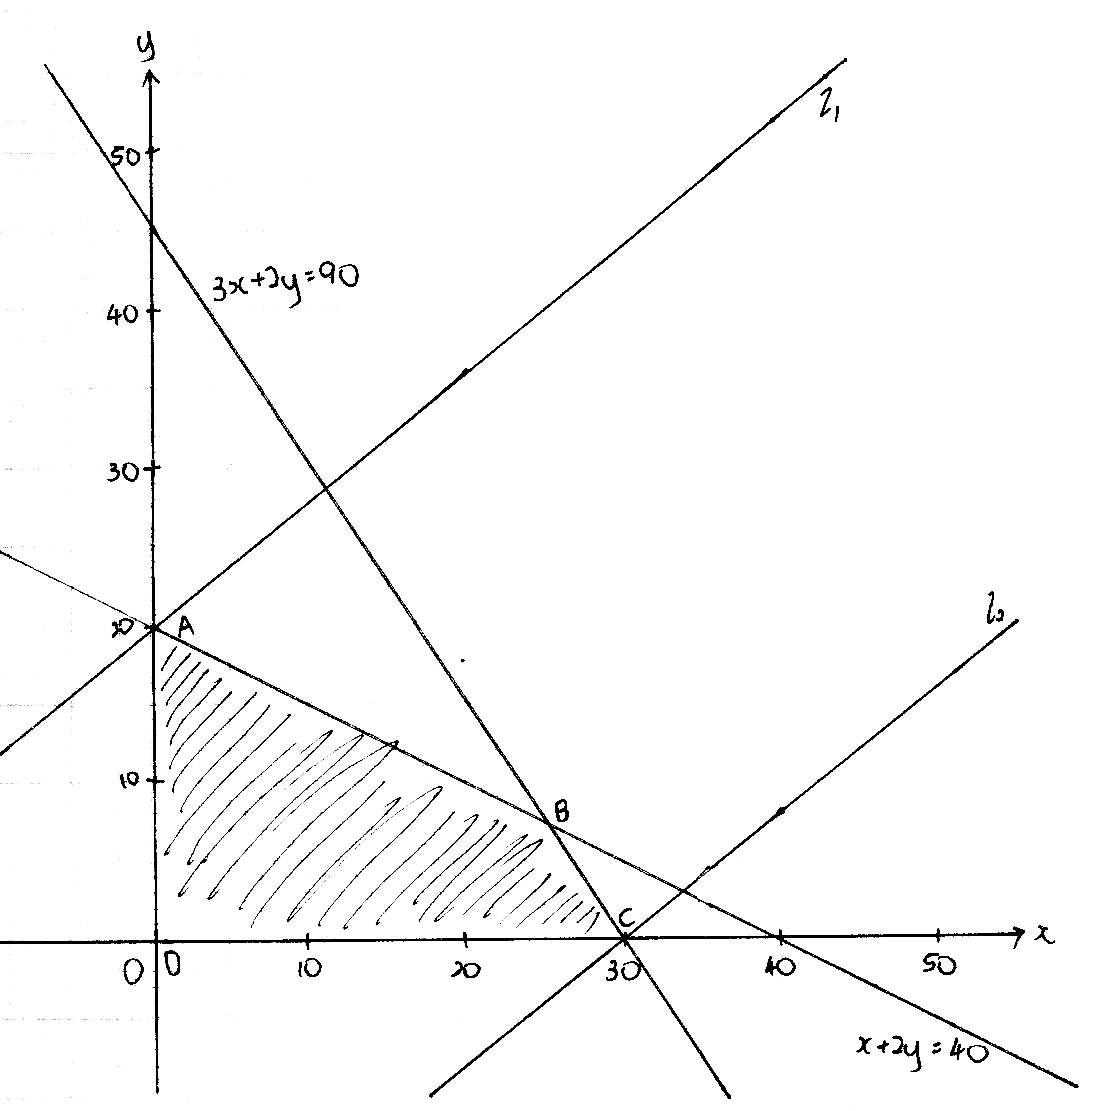
\includegraphics[scale=0.5]{g2}
    \end{center}
    When $y = \frac{4}{5}x - \frac{z}{10}$ translates towards bottom right of the feasible region, the value of $z$ increases. Therefore, the maximum value of the objective function is the value of $z$ in $l_2$. The point of intersection $C$ of $l_2$ and the feasible region makes the objective function to have its maximum value. Since $C$ is also the point of intersection of $3x + 2y = 90$ and $y = 0$,
    \begin{flalign*}
         & \begin{cases}
               3x + 2y = 90 \\
               y = 0
           \end{cases}               \\
         & D = (30, 0)                \\
         & z_{\max} = 8(30) - 0 = 240
    \end{flalign*}
    When $y = x - z$ translates towards top left of the feasible region, the value of $z$ decreases. Therefore, the minimum value of the objective function is the value of $z$ in $l_1$. The point of intersection $A$ of $l_1$ and the feasible region makes the objective function to have its minimum value. Since $A$ is also the point of intersection of $x + 2y = 40$ and $x = 0$,
    \begin{flalign*}
         & \begin{cases}
               x + 2y = 40 \\
               x = 0
           \end{cases}                 \\
         & A = (0, 20)                  \\
         & z_{\min} = 0 - 10(20) = -200
    \end{flalign*}

    \subsection{Exercise 15.8}
    \begin{enumerate}
        \item Find the minimum value of $z = 10x + 12y$, subject to the following
              constraints: \[\begin{cases}
                      3x + y \geq 8   \\
                      2x + 3y \geq 15 \\
                      x + 5y \geq 9   \\
                      x \geq 0        \\
                      y \geq 0
                  \end{cases}\]
              \sol{}
              \begin{flalign*}
                  \text{Objective function: } z & = 10x + 12y                    \\
                  12y                           & = -10x + z                     \\
                  y                             & = -\frac{5}{6}x + \frac{z}{12}
              \end{flalign*}
              \begin{center}
                  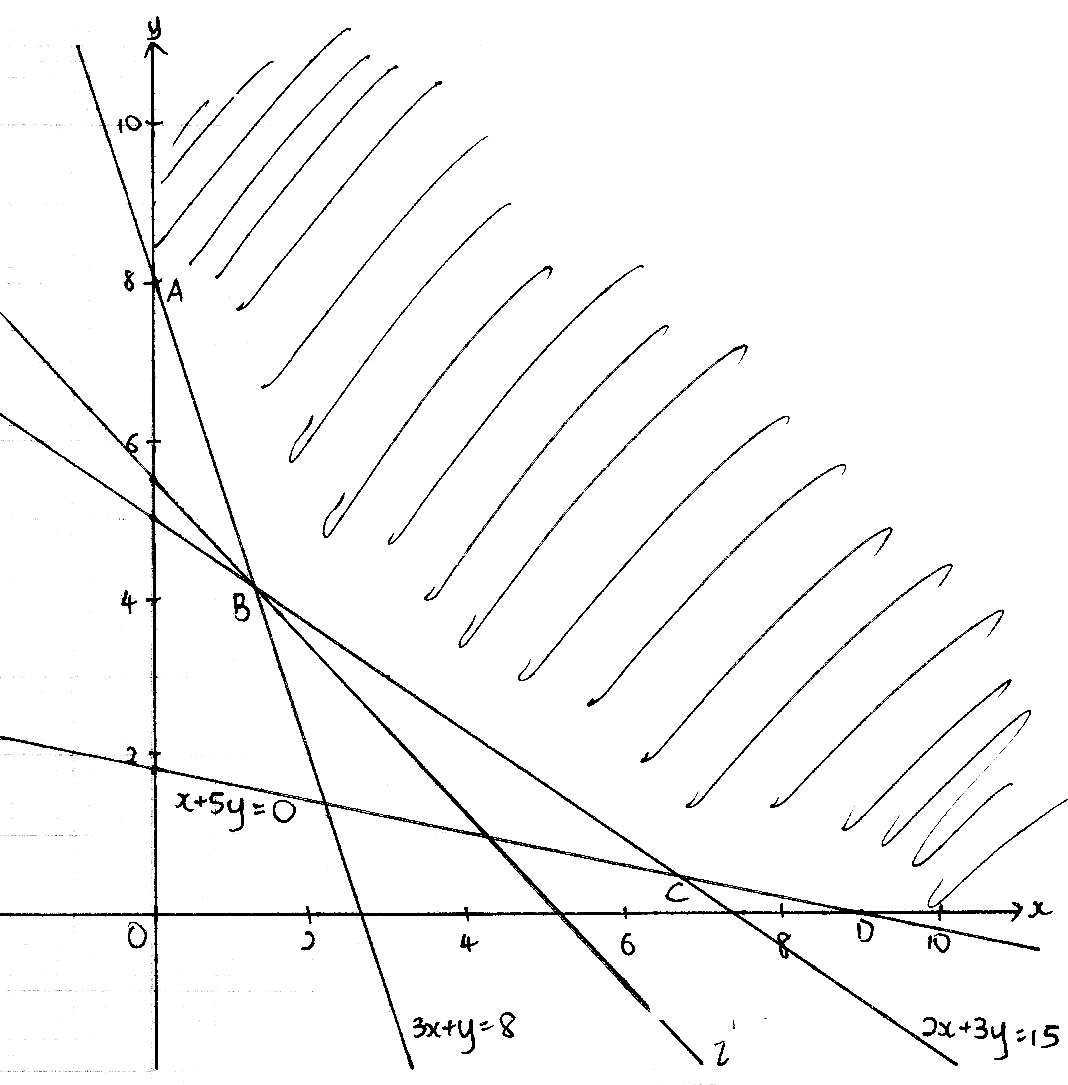
\includegraphics[scale=0.5]{g3}
              \end{center}
              The minimum value of the objective function is the value of $z$ in $l$. The point of intersection $B$ of $l$ and the feasible region makes the objective function to have its minimum value. Since $B$ is also the point of intersection of $3x+y=8$ and $2x+3y=15$,
              \begin{flalign*}
                   & \begin{cases}
                         3x + y = 8 \\
                         2x + 3y = 15
                     \end{cases}
              \end{flalign*}
              \begin{flalign*}
                  2x + 3(8-3x)         & = 15                                 \\
                  2x + 24 - 9x         & = 15                                 \\
                  -7x                  & = -9                                 \\
                  x                    & = \frac{9}{7}                        \\
                  \frac{27}{7} + y     & = 8                                  \\
                  y = 8 - \frac{27}{7} & = \frac{29}{7}                       \\
                  B                    & = (\frac{9}{7}, \frac{29}{7})        \\
                  z_{\min}             & = 10(\frac{9}{7}) + 12(\frac{29}{7}) \\
                                       & = 62\frac{4}{7}
              \end{flalign*}
        \item A housing developer owns a tract of land that is $2,400 m^2$ in area and a
              construction capital of $\$4,600,000$. The developer wishes to build two types
              of houses: type A and type B. Given that each type A house requires $150 m^2$
              of land and $\$250,000$ of construction fees, can earn $\$55,000$ in profit;
              and each type B house requires $200 m^2$ of land and $\$400,000$ of
              construction fees, can earn $\$80,000$ in profit. Assume that all houses built
              can be sold, how many of each type of house should be built to maximize the
              profit? Find the maximum profit. \sol{}

              Let $x$ be the number of type A houses and $y$ be the number of type B houses.
              \begin{center}
                  \begin{tabular}{|c|c|c|c|}
                      \hline
                                   & \textbf{A ($x$ units)} & \textbf{B ($y$ units)} & \textbf{Limit} \\
                      \hline
                      Area ($m^2$) & $150x$                 & $200x$                 & $2,400$        \\
                      Cost(\$)     & $250,000x$             & $400,000y$             & $4,600,000$    \\
                      Profit(\$)   & $55,000x$              & $80,000y$              &                \\
                      \hline
                  \end{tabular}
              \end{center}
              The total profit is $z = 55,000x + 80,000y$, this is the objective function. According to the descriptions above, we find the maximum value of it.

              The constraints are:
              \begin{flalign*}
                  \begin{cases}
                      150x + 200y         \leq 2,400     \\
                      250,000x + 400,000y \leq 4,600,000 \\
                      x                    \geq 0        \\
                      y                   \geq 0
                  \end{cases}
              \end{flalign*}

              After simplifying the constraints, we get:
              \begin{flalign*}
                  \begin{cases}
                      3x + 4y         \leq 48     \\
                      5x + 8y \leq 92             \\
                      x                    \geq 0 \\
                      y                   \geq 0
                  \end{cases}
              \end{flalign*}

              The feasible region is as follows:

              \begin{center}
                  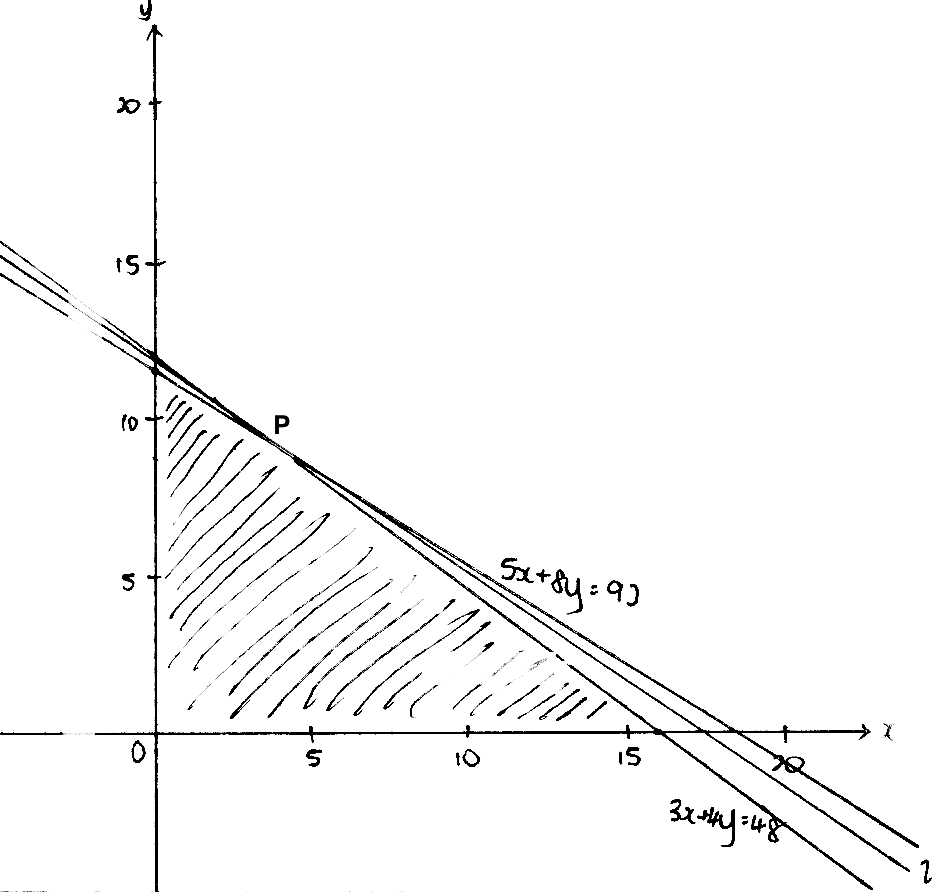
\includegraphics[scale=0.5]{g4}
              \end{center}

              Let $l: 55,000x + 80,000y = z$.

              When the line is at $l$, the value of $z$ is at its maximum. The point of
              intersection $P$ of $l$ and the feasible region makes the objective function to
              have its maximum value. Since $P$ is also the point of intersection of
              $3x+4y=48$ and $5x+8y=92$,

              \setcounter{equation}{0}

              \begin{numcases}{}
                  3x + 4y = 48 \\
                  5x + 8y = 92
              \end{numcases}
              \begin{flalign*}
                  (1) \times 2                       & : 6x + 8y = 96                      \\
                  (1) - (2)                          & : x = 4                             \\
                  \text{Sub } x = 4 \text{ into (1)} & : 12 + 4y = 48                      \\
                                                     & \ \ \ \ \ \ \ \ \ \ \ \ \ \ \ y = 9 \\
                  P                                  & = (4, 9)                            \\
                  z_{\max}                           & = 55,000(4) + 80,000(9)             \\
                                                     & = 940,000
              \end{flalign*}

              Thus, the maximum profit of $\$940,000$ can be obtained by building 4 type A
              houses and 9 type B houses.

        \item One has a building lot that is $180 m^2$ in area. He plans to pay $\$7,000$ to
              split the lot into two type of rooms and rent them out to students: each bigger
              room is $20 m^2$ in area and can accommodate 5 students with a monthly rent of
              $\$225$ per student; each smaller room is $15 m^2$ in area and can accommodate
              3 students with a monthly rent of $\$250$ per student. The renovation cost for
              each bigger room is $\$700$ and for each smaller room is $\$600$. Assume that
              the source of tenants is stable, how many of each type of room should be
              divided into to maximize the profit? Find the maximum profit.

              \sol{}

              Let $x$ be the number of bigger rooms and $y$ be the number of smaller rooms.

              \begin{center}
                  \begin{tabular}{|c|c|c|c|}
                      \hline
                                   & \textbf{Big ($x$ unit)} & \textbf{Small ($y$ unit)} & \textbf{Limit} \\
                      \hline
                      Area ($m^2$) & $20x$                   & $15y$                     & $180$          \\
                      Cost(\$)     & $700x$                  & $600y$                    & $7,000$        \\
                      Profit(\$)   & $1125x$                 & $750y$                    &                \\
                      \hline
                  \end{tabular}
              \end{center}

              The total profit is $z = 1125x + 750y$, this is the objective function.
              According to the descriptions above, we find the maximum value of it.

              The constraints are:

              \begin{flalign*}
                  \begin{cases}
                      20x + 15y \leq 180     \\
                      700x + 600y \leq 7,000 \\
                      x \geq 0               \\
                      y \geq 0
                  \end{cases}
              \end{flalign*}

              After simplifying the constraints, we get:

              \begin{flalign*}
                  \begin{cases}
                      4x + 3y \leq 36 \\
                      7x + 6y \leq 70 \\
                      x \geq 0        \\
                      y \geq 0
                  \end{cases}
              \end{flalign*}

              The feasible region is as follows:

              \begin{center}
                  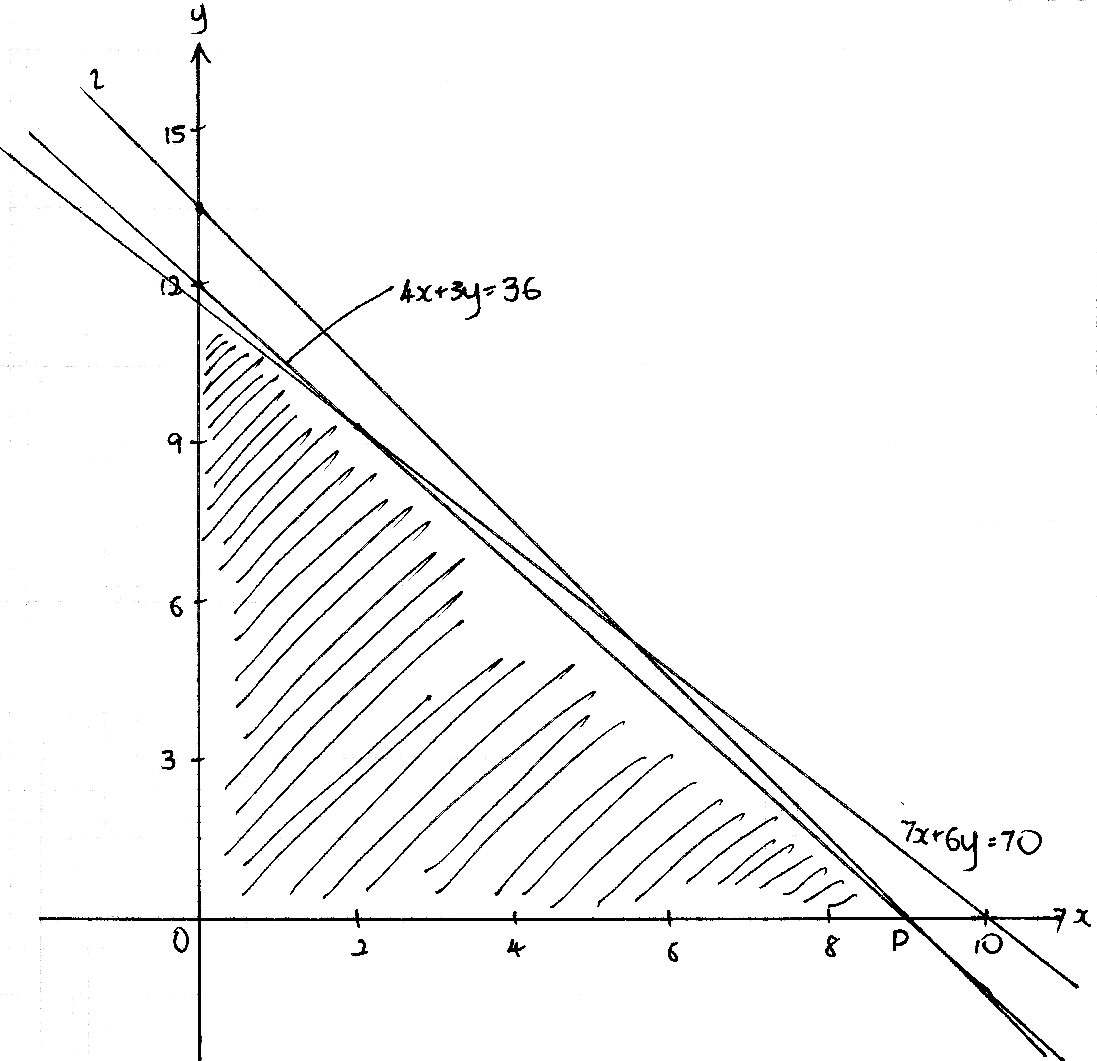
\includegraphics[scale=0.5]{g5}
              \end{center}

              Let $l: 1125x + 750y = z$.

              When the line is at $l$, the value of $z$ is at its maximum. The point of
              intersection $P$ of $l$ and the feasible region makes the objective function to
              have its maximum value. Since $P$ is also the point of intersection of
              $4x+3y=36$ and $y=0$,

              \begin{flalign*}
                   & \begin{cases}
                         4x + 3y = 36 \\
                         y = 0
                     \end{cases}                         \\
                   & P = (9, 0)                           \\
                   & z_{\max} = 1125(9) + 750(0) = 10,125 \\
              \end{flalign*}

              Thus, the maximum profit of $\$10,125$ can be obtained by spliting the building
              lot into 9 bigger rooms.

        \item Ms. Tan is a tuition teacher who teaches Mathematic subject to junior 3 and
              senior 3 students. There are a total of 5 students in each junior 3 class, each
              student pays tuition fees of $\$50$ per month, and each class is held for 4
              hours per week. There are a total of 3 students in each senior 3 class, each
              student pays tuition fees of $\$120$ per month, and each class is held for 6
              hours per week. Assume that here is a stable source of students, but the number
              of junior 3 students cannot exceed 2 times the number of senior 3 students. If
              Ms. Tan is wiling to earn at least $\$6,600$ per month, how many junior 3 and
              senior 3 classes should she held per week to minimize the number hours she has
              to teach? What's the mimimum number of hours she has to teach?

              \sol{}

              Let $x$ be the number of junior 3 classes and $y$ be the number of senior 3
              classes.

              The number of hours she has to teach is $z = 4x + 6y$, this is the objective
              function. According to the descriptions above, we find the minimum value of it.

              The constraints are:

              \begin{flalign*}
                  \begin{cases}
                      5\times 50\times x + 3\times 120\times y \geq 6,600 \\
                      5x \leq 2\times 3y                                  \\
                      x \geq 0                                            \\
                      y \geq 0
                  \end{cases}
              \end{flalign*}

              After simplifying the constraints, we get:

              \begin{flalign*}
                  \begin{cases}
                      25x + 36y \geq 660 \\
                      5x \leq 6y         \\
                      x \geq 0           \\
                      y \geq 0
                  \end{cases}
              \end{flalign*}

              The feasible region is as follows:

              \begin{center}
                  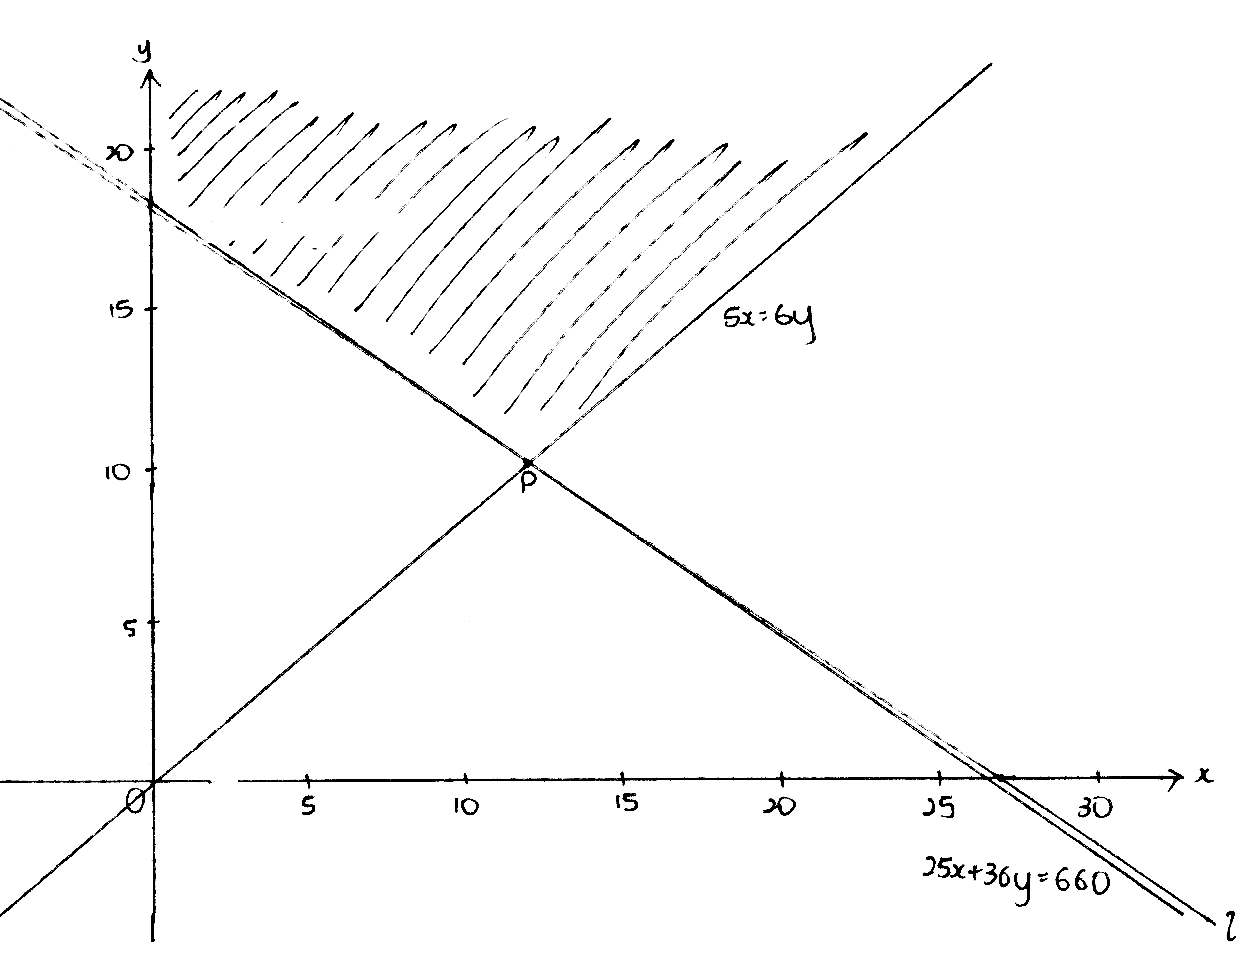
\includegraphics[scale=0.5]{g6}
              \end{center}

              Let $l: 4x + 6y = z$.

              When the line is at $l$, the value of $z$ is at its minimum. The point of
              intersection $P$ of $l$ and the feasible region makes the objective function to
              have its minimum value. Since $P$ is also the point of intersection of $25x +
                  36y = 660$ and $5x = 6y$,

              \setcounter{equation}{0}
              \begin{numcases}{}
                  25x + 36y = 660 \\
                  5x = 6y
              \end{numcases}

              \begin{flalign*}
                  \text{Sub } (2) \text{ into } (1):\     & 25x + 30x = 660                      \\
                                                          & \ \ \ \ \ \ \ \ \ \ \ 55x = 660      \\
                                                          & \ \ \ \ \ \ \ \ \ \ \ \ \ \ \ x = 12 \\
                  \text{Sub } x = 12 \text{ into } (2):\  & 60 = 6y                              \\
                                                          & \ \ y = 10                           \\
                  \\
                  P                                       & = (12, 10)                           \\
                  z_{\min}                                & = 4(12) + 6(10) = 108
              \end{flalign*}

              Thus, Ms. Tan should hold 12 junior 3 classes and 10 senior 3 classes per week,
              and she has to teach for at lest 108 hours per week.

        \item A company can produce a product with two types of raw materials. Each ton of
              the first type of raw material cost $\$300$, freight cost $\$50$, and can
              produce $90kg$ of the product; each ton of the second type of raw material cost
              $\$700$, freight cost $\$40$, and can produce $100kg$ of the product. If the
              company has a total of $\$2,100$ to spend on raw materials and $\$200$ to spend
              on freight every day, what's the maximum amount of product that can be produced
              every day? How many tons of each type of raw material should be used?

              \sol{}

              Let $x$ be the number of tons of the first type of raw material and $y$ be the
              number of tons of the second type of raw material.

              \begin{center}
                  \begin{tabular}{|c|c|c|c|}
                      \hline
                                    & \textbf{M1 ($x$ t)} & \textbf{M2 ($y$ t)} & \textbf{Limit} \\
                      \hline
                      Cost (\$)     & $300x$              & $700y$              & $2,100$        \\
                      Freight(\$)   & $50x$               & $40y$               & $200$          \\
                      Product($kg$) & $90x$               & $100y$              &                \\
                      \hline
                  \end{tabular}
              \end{center}

              The objective function is $z = 90x + 100y$, which is the amount of product that
              can be produced every day. According to the descriptions above, we find the
              maximum value of it.

              The constraints are:

              \begin{flalign*}
                  \begin{cases}
                      300x + 700y \leq 2,100 \\
                      50x + 40y \leq 200     \\
                      x \geq 0               \\
                      y \geq 0
                  \end{cases}
              \end{flalign*}

              After simplifying the constraints, we get:

              \begin{flalign*}
                  \begin{cases}
                      3x + 7y \leq 21 \\
                      5x + 4y \leq 20 \\
                      x \geq 0        \\
                      y \geq 0
                  \end{cases}
              \end{flalign*}

              The feasible region is as follows:

              \begin{center}
                  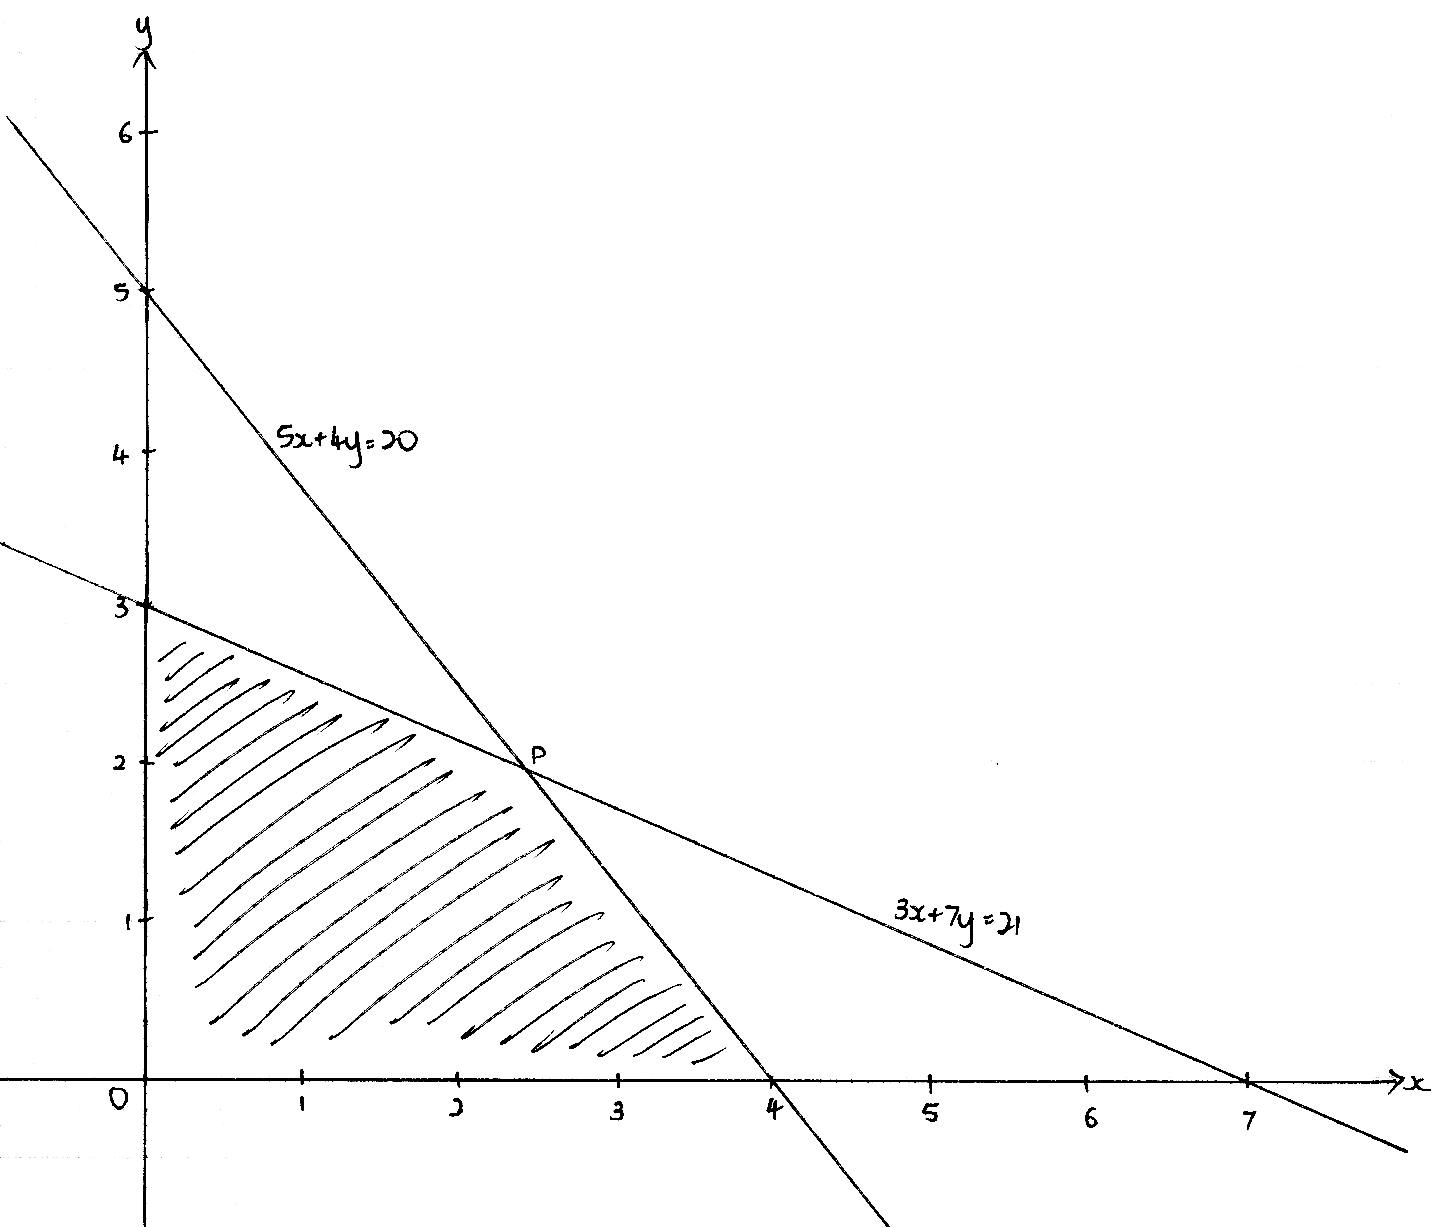
\includegraphics[scale=0.5]{g7}
              \end{center}

              Let $l: 90x + 100y = z$.

              When the line is at $l$, the value of $z$ is at its maximum. The point of
              intersection $P$ of $l$ and the feasible region makes the objective function to
              have its maximum value. Since $P$ is also the point of intersection of $3x + 7y
                  = 21$ and $5x + 4y = 20$,

              \setcounter{equation}{0}
              \begin{numcases}{}
                  3x + 7y = 21 \\
                  5x + 4y = 20
              \end{numcases}

              \begin{flalign*}
                  (1) \times 5:                                    & \ 15x + 35y = 105                                              \\
                  (2) \times 3:                                    & \ 15x + 12y = 60                                               \\
                  (1) - (2):                                       & \ 23y = 45                                                     \\
                                                                   & \ \ \ \ \  y = \frac{45}{23}                                   \\
                                                                   & \ \ \ \ \ \ \  = 1.96                                          \\
                  \text{Sub } y = \frac{45}{23} \text{ into } (2): & \ 5x + \frac{180}{23} = 20                                     \\
                                                                   & \ \ \ \ \ \ \ \ \ \ \ \ \ 5x = \frac{280}{23}                  \\
                                                                   & \ \ \ \ \ \ \ \ \ \ \ \ \ \ \ x = \frac{56}{23}                \\
                                                                   & \ \ \ \ \ \ \ \ \ \ \ \ \ \ \ \ \ = 2.43                       \\
                  \\
                  P                                                & = (2.43, 1.96)                                                 \\
                  z_{\max}                                         & = 90\left(\frac{56}{23}\right) + 100\left(\frac{45}{23}\right) \\
                                                                   & = 414.78
              \end{flalign*}

              Thus, the company should use $2.43$ tons of the first type of raw material and
              $1.96$ tons of the second type of raw material, and the maximum amount of
              product that can be produced every day is $414.78 kg$.

        \item A factory uses four types of raw materials: $a$, $b$, $c$, and $d$ to produce
              two types of products: $A$ and $B$, the stock of raw materials $a$, $b$, $c$,
              and $d$ are 22, 14, 15, and 18 units respectively. Given that the required
              amount of raw materials $a$, $b$, $c$, and $d$ for producing one unit of
              product $A$ is 3, 2, 0, 3 units respectively, and the required amount of raw
              materials $a$, $b$, $c$, and $d$ for producing one unit of product $B$ is 2, 1,
              3, 0 units respectively. If each product $A$ can make a profit of $\$7,000$ and
              each product $B$ can make a profit of $\$5,000$, how many units of each product
              should be produced to maximize the profit with the current stock of raw
              materials?

              \sol{}

              Let $x$ be the number of units of product $A$ and $y$ be the number of units of
              product $B$.

              \begin{center}
                  \begin{tabular}{|c|c|c|c|}
                      \hline
                                  & \textbf{A ($x$ unit)} & \textbf{B ($y$ unit)} & \textbf{Limit} \\
                      \hline
                      $a$ (unit)  & $3x$                  & $2y$                  & $22$           \\
                      $b$ (unit)  & $2x$                  & $y$                   & $14$           \\
                      $c$ (unit)  & $0x$                  & $3y$                  & $15$           \\
                      $d$ (unit)  & $3x$                  & $0y$                  & $18$           \\
                      Profit (\$) & $7,000x$              & $5,000y$              &                \\
                      \hline
                  \end{tabular}
              \end{center}

              The objective function is $z = 7,000x + 5,000y$, which is the profit. According
              to the descriptions above, we find the maximum value of it. The constraints
              are:

              \begin{flalign*}
                  \begin{cases}
                      3x + 2y \leq 22 \\
                      2x + y \leq 14  \\
                      3y \leq 15      \\
                      3x \leq 18      \\
                      x \geq 0        \\
                      y \geq 0
                  \end{cases}
              \end{flalign*}

              After simplifying the constraints, we get:

              \begin{flalign*}
                  \begin{cases}
                      3x + 2y \leq 22 \\
                      2x + y \leq 14  \\
                      0 \leq y \leq 5 \\
                      0 \leq x \leq 6 \\
                  \end{cases}
              \end{flalign*}

              The feasible region is as follows:

              \begin{center}
                  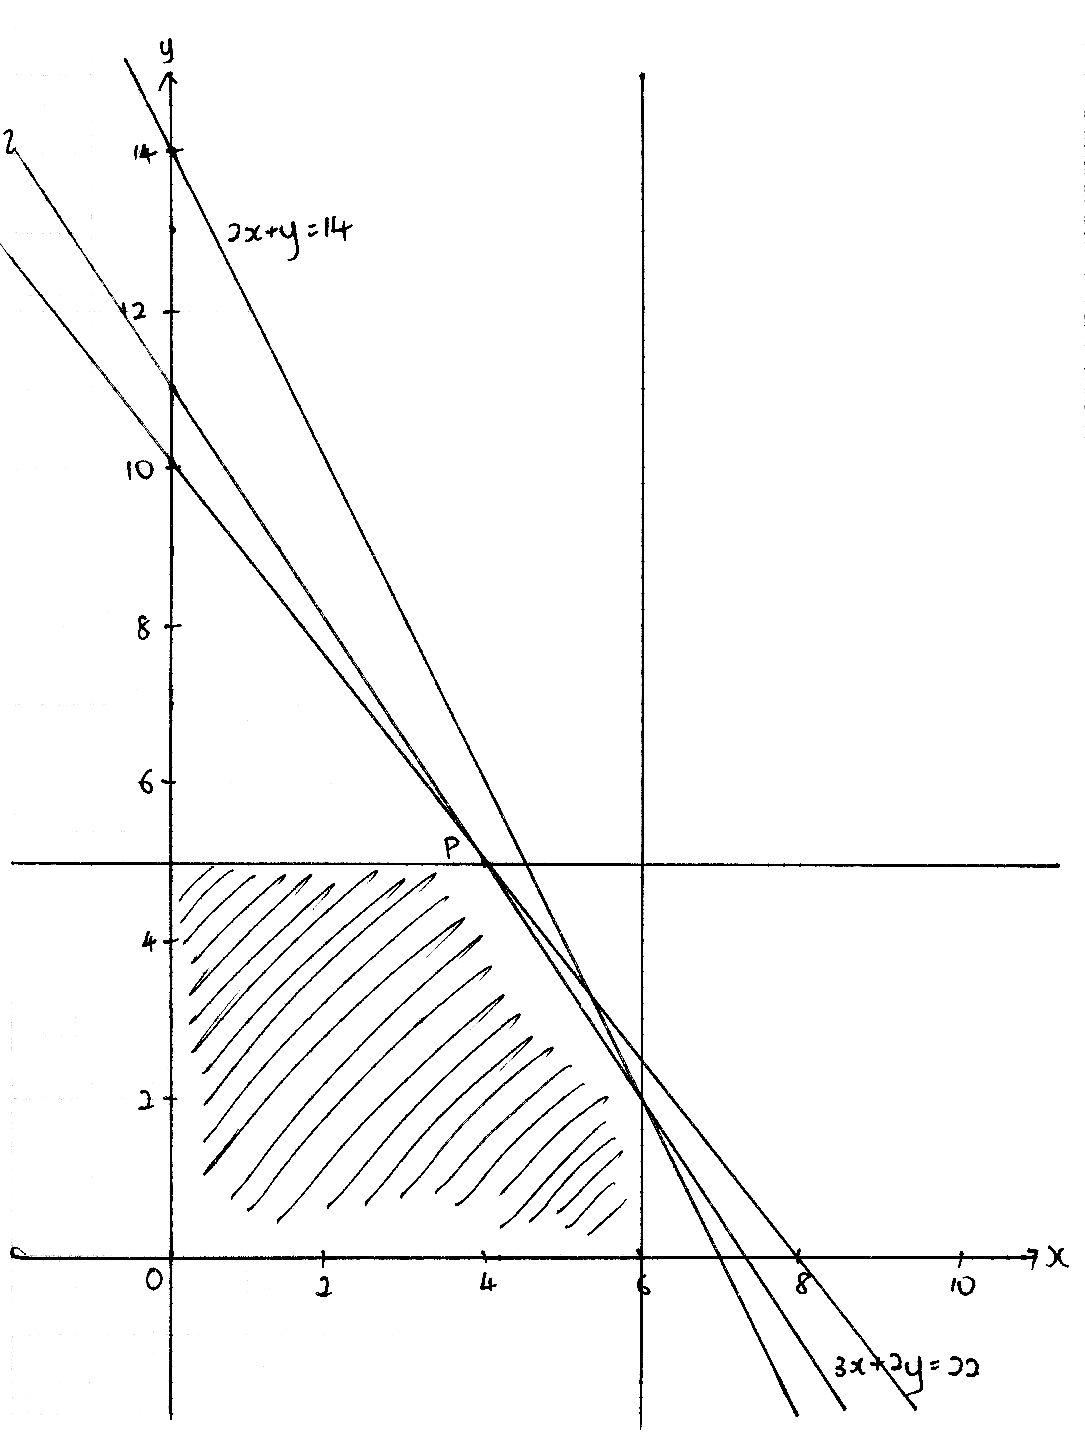
\includegraphics[scale=0.5]{g8}
              \end{center}

              Let $l: 7,000x + 5,000y = z$.

              When the line is at $l$, the value of $z$ is at its maximum. The point of
              intersection $P$ of $l$ and the feasible region makes the objective function to
              have its maximum value. Since $P$ is also the point of intersection of $3x + 2y
                  = 22$ and $y = 5$,

              \begin{flalign*}
                   & \begin{cases}
                         3x + 2y = 22 \\
                         y = 5
                     \end{cases} \\
                   & P = (4, 5)
              \end{flalign*}

              Thus, the company should produce $4$ units of product $A$ and $5$ units of
              product $B$ to maximize the profit.

        \item Mr. Wong is willing to mix two types of drinks: $A$ and $B$ to produce a new
              drink. Drink $A$ cost $\$2$ per litre, contains $20mg$ of vitamin $C$, $3mg$ of
              coloring agent, and $150g$ of sugar; drink $B$ cost $\$4$ per litre, contains
              $35mg$ of vitamin $C$, $2mg$ of coloring agent, and $100g$ of sugar. Mr. Tan is
              willing to mix at least $50$ litres of the new drink, but each litre of the new
              drink has to contain at least $30mg$ of vitamin $C$, the total amount of sugar
              cannot exceed $6kg$, and the total cost cannot exceed $\$180$. How many litres
              of each type of drink should be mixed to minimize the amount of coloring agent?

              \sol{}

              Let $x$ be the number of litres of drink $A$ and $y$ be the number of litres of
              drink $B$.

              The objective function is $z = 3x + 2y$, which is the amount of coloring agent.
              According to the descriptions above, we find the minimum value of it. The
              constraints are:

              \begin{flalign*}
                  \begin{cases}
                      x + y \geq 50          \\
                      20x + 35y \geq 30(x+y) \\
                      150x + 100y \leq 6,000 \\
                      2x + 4y \leq 180       \\
                      x \geq 0               \\
                      y \geq 0
                  \end{cases}
              \end{flalign*}

              After simplifying the constraints, we get:

              \begin{flalign*}
                  \begin{cases}
                      x + y \geq 50    \\
                      -2x + y \geq 0   \\
                      3x + 2y \leq 120 \\
                      x + 2y \leq 90   \\
                      x \geq 0         \\
                      y \geq 0
                  \end{cases}
              \end{flalign*}

              The feasible region is as follows:

              \begin{center}
                  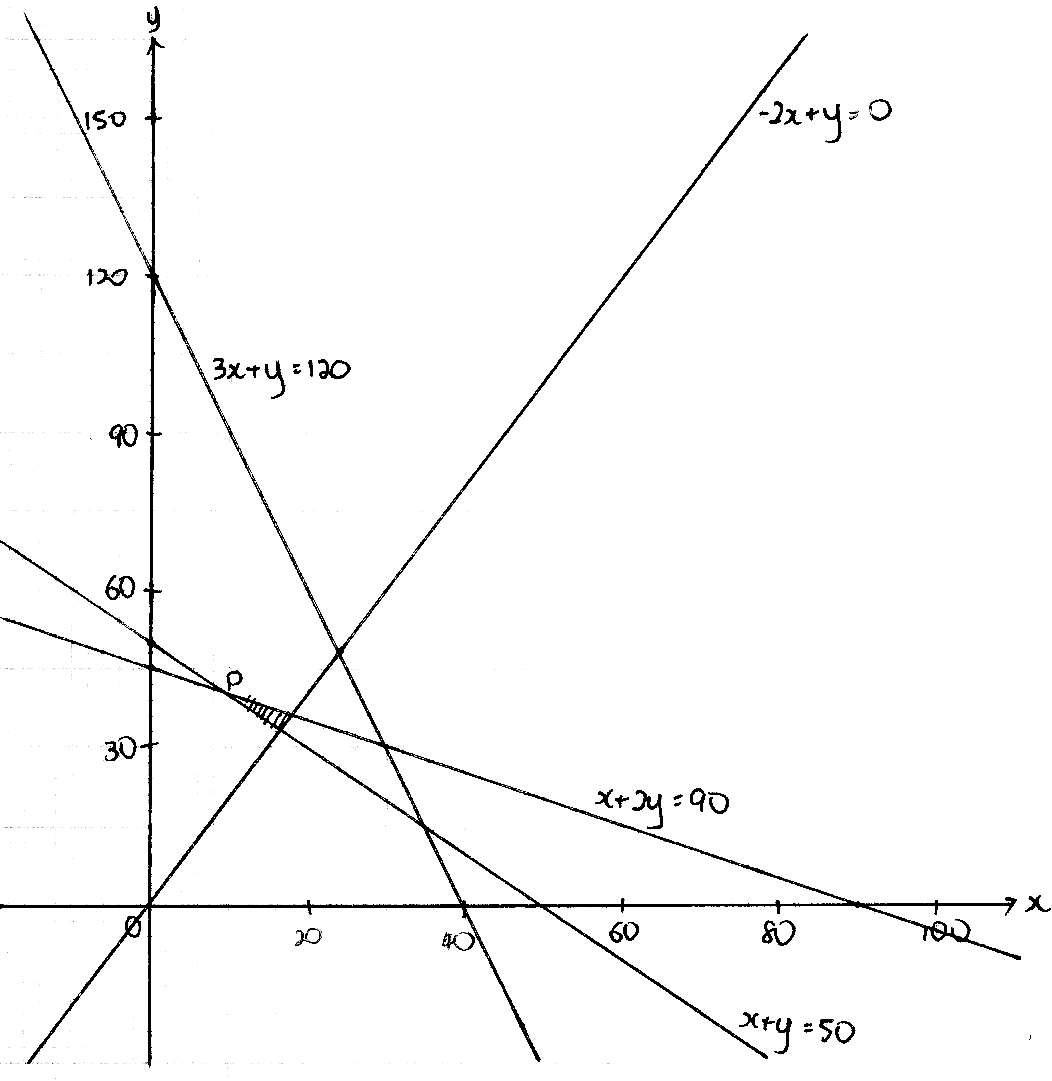
\includegraphics[scale=0.5]{g9}
              \end{center}

              Let $l: 3x + 2y = z$.

              When the line is at $l$, the value of $z$ is at its minimum. The point of
              intersection $P$ of $l$ and the feasible region makes the objective function to
              have its minimum value. Since $P$ is also the point of intersection of $x + y =
                  50$ and $x + 2y = 90$,

              \begin{flalign*}
                   & \begin{cases}
                         x + y = 50 \\
                         x + 2y = 90
                     \end{cases} \\
                   & P = (10, 40)
              \end{flalign*}

              Thus, the company should produce $10$ litres of drink $A$ and $40$ litres of
              drink $B$ to minimize the amount of coloring agent.

        \item A bakery bakes two types of cake: $A$ and $B$. The ingredients required for
              baking one cake of type $A$ is $1kg$ of flour, 5 eggs, and $300g$ of sugar; the
              ingredients required for baking one cake of type $B$ is $800g$ of flour, 8
              eggs, and $200g$ of sugar. The bakery has 3 bakers, each of them works for at
              least 8 hours per day, and the total time required for each baker to bake one
              cake of type $A$ and $B$ is 40 minutes and 50 minutes respectively. If the
              bakery has to bake at least 32 cakes every day, and the everyday supply of
              ingredients is limited to 220 eggs and $9kg$ of sugar. Due to the shortage of
              flour, the bakery needs to lower the usage of it. How many cakes of each type
              should be baked to minimize the usage of flour? What's the minimum amount of
              flour used?

              \sol{}

              Let $x$ be the number of cakes of type $A$ and $y$ be the number of cakes of
              type $B$.

              The objective function is $z = x + 0.8y$, which is the amount of flour used.
              According to the descriptions above, we find the minimum value of it. The
              constraints are:

              \begin{flalign*}
                  \begin{cases}
                      5x + 8y \leq 220       \\
                      300x + 200y \leq 9,000 \\
                      40x + 50y \geq 480     \\
                      x + y \geq 32          \\
                      x \geq 0               \\
                      y \geq 0
                  \end{cases}
              \end{flalign*}

              After simplifying the constraints, we get:
              \begin{flalign*}
                  \begin{cases}
                      5x + 8y \leq 220 \\
                      3x + 2y \leq 90  \\
                      4x + 5y \geq 120 \\
                      x + y \geq 32    \\
                      x \geq 0         \\
                      y \geq 0
                  \end{cases}
              \end{flalign*}

              The feasible region is as follows:

              \begin{center}
                  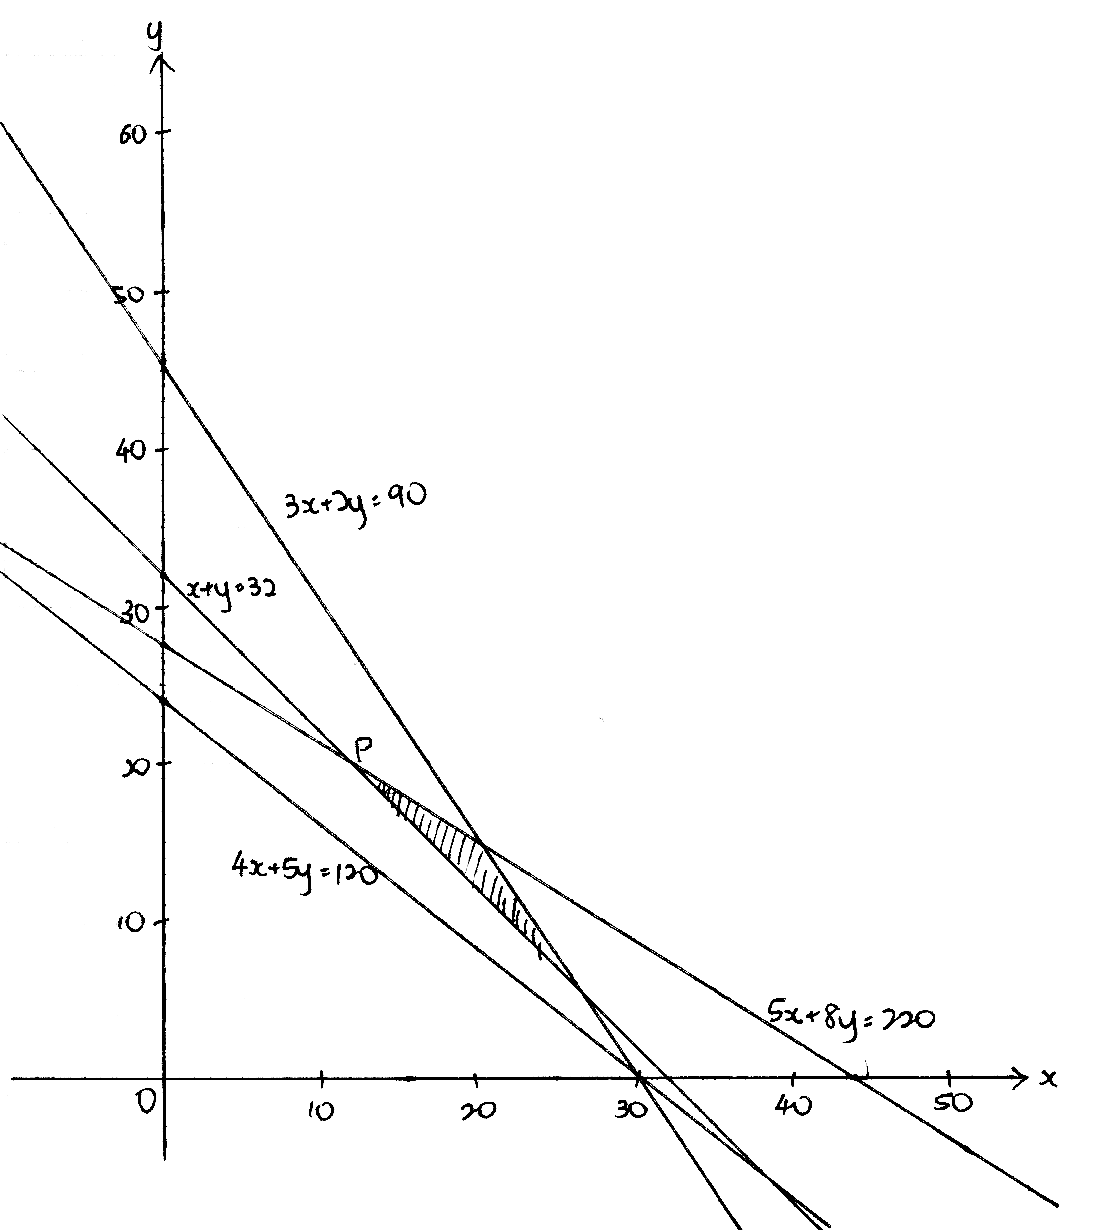
\includegraphics[scale=0.5]{g10}
              \end{center}

              Let $l: 4x + 5y = z$.

              When the line is at $l$, the value of $z$ is at its minimum. The point of
              intersection $P$ of $l$ and the feasible region makes the objective function to
              have its minimum value. Since $P$ is also the point of intersection of $x + y =
                  32$ and $5x + 8y = 220$,

              \setcounter{equation}{0}
              \begin{numcases}{}
                  x + y = 32 \\
                  5x + 8y = 220
              \end{numcases}

              \begin{flalign*}
                  (1):                               & \ y = 32 - x (3)                                       \\
                  \text{Sub } (3) \text{ into } (2): & \ 5x + 8(32-x) = 220                                   \\
                                                     & \ \ 5x + 256 - 8x = 220                                \\
                                                     & \ \ \ \ \ \ \ \ \ \ \ \ \ \ \ \ \ -3x = -36            \\
                                                     & \ \ \ \ \ \ \ \ \ \ \ \ \ \ \ \ \ \ \ \ \ \ \ \ x = 12 \\
                                                     & \ \ \ \ \ \ \ \ \ \ \ \ \ \ \ \ \ \ \ \ \ \ \ \ y = 20 \\
                  \\
                  P                                  & = (12, 20)                                             \\
                  z                                  & = 12 + 0.8(20) = 28
              \end{flalign*}

              Thus, the bakery should bake $12$ cakes of type $A$ and $20$ cakes of type $B$
              to minimize the amount of flour used. The minimum amount of flour used is
              $28kg$
    \end{enumerate}

    \section{Revision Exercise 15}

    Compare the algebraic expressions in the following questions (Question 1 to 2):
    \begin{enumerate}
        \item $(x-3)(4-x)$ and $(6-x)(x-1)$
              \sol{}
              \begin{flalign*}
                             & (x-3)(4-x) - (6-x)(x-1)            \\
                             & = -x^2 + 7x - 12 - (-x^2 + 7x - 6) \\
                             & = -x^2 + 7x - 12 + x^2 - 7x + 6    \\
                             & = -6 < 0                           \\
                  \therefore & \  (x-3)(4-x) < (6-x)(x-1)
              \end{flalign*}
        \item $6 - x^2$ and $4x - 2x^2$
              \sol{}
              \begin{flalign*}
                             & 6 - x^2 - (4x - 2x^2)  \\
                             & = 6x - x^2 - 4x + 2x^2 \\
                             & = x^2 - 2x             \\
                             & = {(x - 1)}^2 + 1      \\
                  \because   & \ {(x - 1)}^2 + 1 > 0  \\
                  \therefore & \ {(x - 1)}^2 + 1 > 0  \\
                  \therefore & \ 6 - x^2 > 4x - 2x^2
              \end{flalign*}
    \end{enumerate}

    \noindent Solve the following inequalities (Question 3 to 16):
    \begin{enumerate}
        \setcounter{enumi}{2}
        \item $4(x-1) > x+6$
              \sol{}
              \begin{flalign*}
                  4(x-1) & > x+6          \\
                  4x - 4 & > x+6          \\
                  3x     & > 10           \\
                  x      & > \frac{10}{3}
              \end{flalign*}
        \item $3(3-x) \geq 2(x+3)$
              \sol{}
              \begin{flalign*}
                  3(3-x) & \geq 2(x+3)      \\
                  9 - 3x & \geq 2x + 6      \\
                  -5x    & \geq -3          \\
                  5x     & \leq 3           \\
                  x      & \leq \frac{3}{5}
              \end{flalign*}
        \item $3-\frac{x-1}{4} \geq 2+\frac{3(x+1)}{8}$
              \sol{}
              \begin{flalign*}
                  3 - \frac{x-1}{4} & \geq 2 + \frac{3(x+1)}{8} \\
                  24 - 2(x-1)       & \geq 16 + 3(x+1)          \\
                  24 - 2x + 2       & \geq 16 + 3x + 3          \\
                  26 - 2x           & \geq 19 + 3x              \\
                  -5x               & \geq -7                   \\
                  5x                & \leq 7                    \\
                  x                 & \leq \frac{7}{5}
              \end{flalign*}
        \item $x-\frac{x-1}{2} \leq \frac{2x-1}{3} + \frac{x+1}{2}$
              \sol{}
              \begin{flalign*}
                  x - \frac{x-1}{2} & \leq \frac{2x-1}{3} + \frac{x+1}{2} \\
                  6x - 3(x-1)       & \leq 2(2x-1) + 3(x+1)               \\
                  6x - 3x + 3       & \leq 4x - 2 + 3x + 3                \\
                  3x + 3            & \leq 7x + 1                         \\
                  -4x               & \leq -2                             \\
                  4x                & \geq 2                              \\
                  x                 & \geq \frac{1}{2}
              \end{flalign*}
        \item $-1 < \frac{1}{2}x + 3 < 7$
              \sol{}
              \begin{flalign*}
                  -1 < \frac{1}{2}x & + 3 < 7  \\
                  -2 < x            & + 6 < 14 \\
                  -8 <              & \ x < 8
              \end{flalign*}
        \item $-\frac{3}{2} < 1 - 3x \leq 8$
              \sol{}
              \begin{flalign*}
                  -\frac{3}{2} & < 1 - 3x \leq 8      \\
                  -3           & < 2 - 6x \leq 16     \\
                  -5           & < -6x \leq 14        \\
                  -14          & \leq 6x < 5          \\
                  -\frac{7}{3} & \leq x < \frac{5}{6}
              \end{flalign*}
        \item $x^2 < 7$
              \sol{}
              \begin{flalign*}
                  x^2                      & < 7        \\
                  x^2 - 7                  & < 0        \\
                  (x+\sqrt{7})(x-\sqrt{7}) & < 0        \\
                  -\sqrt{7} < x            & < \sqrt{7}
              \end{flalign*}
              \begin{center}
                  \begin{tikzpicture}
                      \draw[latex-latex] (0,0) -- (6,0);
                      \draw[shift={(2,0)},color=black] (0pt,3pt) -- (0pt,-3pt) node[below] {$-\sqrt{7}$};
                      \draw[shift={(4,0)},color=black] (0pt,3pt) -- (0pt,-3pt) node[below] {$\sqrt{7}$};
                      \draw[shift={(1,0)},color=black] node[above] {$+$};
                      \draw[shift={(3,0)},color=black] node[above] {$-$};
                      \draw[shift={(5,0)},color=black] node[above] {$+$};
                      \node[circle,draw,fill=white,inner sep=1.5pt](a)at(2,1){};
                      \draw (a)--(4,1);
                      \node[circle,draw,fill=white,inner sep=1.5pt](b)at(4,1){};
                  \end{tikzpicture}
              \end{center}
        \item $x^2 + 10x - 200 \geq 0$
              \sol{}
              \begin{flalign*}
                  x^2 + 10x - 200               & \geq 0  \\
                  (x+20)(x-10)                  & \geq 0  \\
                  x \leq -20      \text{ or } x & \geq 10
              \end{flalign*}
              \begin{center}
                  \begin{tikzpicture}
                      \draw[latex-latex] (0,0) -- (6,0);
                      \draw[shift={(2,0)},color=black] (0pt,3pt) -- (0pt,-3pt) node[below] {$-20$};
                      \draw[shift={(4,0)},color=black] (0pt,3pt) -- (0pt,-3pt) node[below] {$10$};
                      \draw[shift={(3,0)},color=black] node[above] {$-$};
                      \draw[shift={(1,0)},color=black] node[above] {$+$};
                      \draw[shift={(5,0)},color=black] node[above] {$+$};
                      \node[circle,fill,inner sep=1.5pt](a)at(4,1){};
                      \node[circle,fill,inner sep=1.5pt](b)at(2,1){};
                      \draw[-latex,black](a)--(6,1);
                      \draw[-latex,black](b)--(0,1);
                  \end{tikzpicture}
              \end{center}
        \item $4 < 3x^2 + 4x$
              \sol{}
              \begin{flalign*}
                  4             & < 3x^2 + 4x                 \\
                  3x^2 + 4x - 4 & > 0                         \\
                  (3x-2)(x+2)   & > 0                         \\
                  x < -2        & \text{ or } x > \frac{2}{3}
              \end{flalign*}
              \begin{center}
                  \begin{tikzpicture}
                      \draw[latex-latex] (0,0) -- (6,0);
                      \draw[shift={(2,0)},color=black] (0pt,3pt) -- (0pt,-3pt) node[below] {$-2$};
                      \draw[shift={(4,0)},color=black] (0pt,3pt) -- (0pt,-3pt) node[below] {$\frac{2}{3}$};
                      \draw[shift={(1,0)},color=black] node[above] {$+$};
                      \draw[shift={(3,0)},color=black] node[above] {$-$};
                      \draw[shift={(5,0)},color=black] node[above] {$+$};
                      \node[circle,draw,fill=white,inner sep=1.5pt](a)at(2,1){};
                      \node[circle,draw,fill=white,inner sep=1.5pt](b)at(4,1){};
                      \draw[-latex,black](a)--(0,1);
                      \draw[-latex,black](b)--(6,1);
                  \end{tikzpicture}
              \end{center}
        \item $5x - 3 \geq 2x^2$
              \sol{}
              \begin{flalign*}
                  5x - 3        & \geq 2x^2        \\
                  2x^2 - 5x + 3 & \leq 0           \\
                  (2x-3)(x-1)   & \leq 0           \\
                  1 \leq x      & \leq \frac{3}{2}
              \end{flalign*}
              \begin{center}
                  \begin{tikzpicture}
                      \draw[latex-latex] (0,0) -- (6,0);
                      \draw[shift={(2,0)},color=black] (0pt,3pt) -- (0pt,-3pt) node[below] {$1$};
                      \draw[shift={(4,0)},color=black] (0pt,3pt) -- (0pt,-3pt) node[below] {$\frac{3}{2}$};
                      \draw[shift={(1,0)},color=black] node[above] {$+$};
                      \draw[shift={(3,0)},color=black] node[above] {$-$};
                      \draw[shift={(5,0)},color=black] node[above] {$+$};
                      \node[circle,fill,inner sep=1.5pt](a)at(2,1){};
                      \draw (a)--(4,1);
                      \node[circle,fill,inner sep=1.5pt](b)at(4,1){};
                  \end{tikzpicture}
              \end{center}
        \item $x^2 - x(x-6) > 5(x-1)$
              \sol{}
              \begin{flalign*}
                  x^2 - x(x-6)   & > 5(x-1) \\
                  x^2 - x^2 + 6x & > 5x - 5 \\
                  6x             & > 5x - 5 \\
                  x              & > -5
              \end{flalign*}
        \item ${(2x+1)}^2 + 5 \leq 4{(x+2)}^2$
              \sol{}
              \begin{flalign*}
                  {(2x+1)}^2 + 5    & \leq 4{(x+2)}^2      \\
                  4x^2 + 4x + 1 + 5 & \leq 4(x^2 + 4x + 4) \\
                  4x^2 + 4x + 6     & \leq 4x^2 + 16x + 16 \\
                  -12x              & \leq 10              \\
                  12x               & \geq -10             \\
                  x                 & \geq -\frac{5}{6}
              \end{flalign*}
        \item $9x^2 + 2 \leq 12x - 2$
              \sol{}
              \begin{flalign*}
                  9x^2 + 2       & \leq 12x - 2  \\
                  9x^2 - 12x + 4 & \leq 0        \\
                  {(3x - 2)}^2   & \leq 0        \\
                  x              & = \frac{2}{3}
              \end{flalign*}
        \item $4(x^2 + 7) > 3 - 20x$
              \sol{}
              \begin{flalign*}
                  4(x^2 + 7)         & > 3 - 20x             \\
                  4x^2 + 28          & > 3 - 20x             \\
                  4x^2 + 20x - 25    & > 0                   \\
                  {(2x + 5)}^2       & > 0                   \\
                  x \in \mathbb{R} , & \ x \neq -\frac{5}{2}
              \end{flalign*}
    \end{enumerate}

    \noindent Solve the following system of inequalities (Question 17 to 28):

    \begin{enumerate}
        \setcounter{enumi}{16}
        \setcounter{equation}{0}
        \item \begin{numcases}{}
                  3x + 2 \leq{0} \\
                  4-x < x
              \end{numcases}
              \sol{}
              \begin{flalign*}
                  (1):\        & 3x \leq -2          \\
                               & x \leq -\frac{2}{3} \\
                  (2):\        & -2x < -4            \\
                               & x > 2               \\
                  \\
                  \therefore\  & \text{No solution.}
              \end{flalign*}
              \begin{center}
                  \begin{tikzpicture}
                      \draw[latex-latex] (0,0) -- (6,0);
                      \draw[shift={(2,0)},color=black] (0pt,3pt) -- (0pt,-3pt) node[below] {$-\frac{2}{3}$};
                      \draw[shift={(4,0)},color=black] (0pt,3pt) -- (0pt,-3pt) node[below] {2};
                      \node[circle,fill=black,inner sep=1.5pt](a)at(2,1){};
                      \draw[-latex] (a)--(0,1);
                      \node[circle,draw,fill=white,inner sep=1.5pt](b)at(4,1){};
                      \draw[-latex] (b) -- (6, 1);
                  \end{tikzpicture}
              \end{center}

              \setcounter{equation}{0}
        \item \begin{numcases}{}
                  x + 4 > -x \\
                  \frac{3x -1}{2} < 2(x+1)
              \end{numcases}
              \sol{}
              \begin{flalign*}
                  (1):\        & 2x > -4         \\
                               & x > -2          \\
                  (2):\        & 3x - 1 < 4(x+1) \\
                               & 3x - 1 < 4x + 4 \\
                               & -x < 5          \\
                               & x > -5          \\
                  \\
                  \therefore\  & x > -2
              \end{flalign*}
              \begin{center}
                  \begin{tikzpicture}
                      \fill[gray!40] (4,0) rectangle (6,1.5);
                      \draw[latex-latex] (0,0) -- (6,0);
                      \draw[shift={(2,0)},color=black] (0pt,3pt) -- (0pt,-3pt) node[below] {$-5$};
                      \draw[shift={(4,0)},color=black] (0pt,3pt) -- (0pt,-3pt) node[below] {$-2$};
                      \node[circle,draw,fill=white,inner sep=1.5pt](a)at(2,1){};
                      \draw[-latex] (a)--(6,1);
                      \node[circle,draw,fill=white,inner sep=1.5pt](b)at(4,1.5){};
                      \draw[-latex] (b) -- (6, 1.5);
                  \end{tikzpicture}
              \end{center}

              \setcounter{equation}{0}
        \item \begin{numcases}{}
                  x -3 \leq{5 -3x} \\
                  4 + (2x -1) \leq{4x + 7}
              \end{numcases}
              \sol{}
              \begin{flalign*}
                  (1):\        & 4x \leq 8          \\
                               & x \leq 2           \\
                  (2):\        & 3 + 2x \leq 4x + 7 \\
                               & -2x \leq 4         \\
                               & x \geq -2          \\
                  \\
                  \therefore\  & -2 \leq x \leq 2
              \end{flalign*}
              \begin{center}
                  \begin{tikzpicture}
                      \fill[black!20](2,0)rectangle(4,1.5);
                      \draw[latex-latex] (0,0) -- (6,0) ;
                      \draw[shift={(2,0)},color=black] (0pt,3pt) -- (0pt,-3pt) node[below] {$-2$};
                      \draw[shift={(4,0)},color=black] (0pt,3pt) -- (0pt,-3pt) node[below] {$2$};
                      \node[circle,fill,inner sep=1.5pt](a)at(4,1.5){};
                      \node[circle,fill,inner sep=1.5pt](b)at(2,1){};
                      \draw[-latex,black](a)--(0,1.5);
                      \draw[-latex,black](b)--(6,1);
                  \end{tikzpicture}
              \end{center}

              \setcounter{equation}{0}
        \item \begin{numcases}{}
                  4x -5 \geq{2x + 1} \\
                  x + \frac{2}{3} \leq{\frac{2x + 5}{3}}
              \end{numcases}
              \sol{}
              \begin{flalign*}
                  (1): \       & 2x \geq 6          \\
                               & x \geq 3           \\
                  (2): \       & 3x + 2 \leq 2x + 5 \\
                               & x \leq 3           \\
                  \\
                  \therefore\  & x = 3
              \end{flalign*}
              \begin{center}
                  \begin{tikzpicture}
                      \fill[black!20](2.9,0)rectangle(3.1,1.5);
                      \draw[latex-latex] (0,0) -- (6,0) ;
                      \draw[shift={(3,0)},color=black] (0pt,3pt) -- (0pt,-3pt) node[below] {$3$};
                      \node[circle,fill,inner sep=1.5pt](a)at(3,1.5){};
                      \node[circle,fill,inner sep=1.5pt](b)at(3,1){};
                      \draw[-latex,black](a)--(0,1.5);
                      \draw[-latex,black](b)--(6,1);
                  \end{tikzpicture}
              \end{center}

              \setcounter{equation}{0}
        \item $5 < 2x - 7 < x + 1$
              \sol{}
              \begin{numcases}{}
                  5 < 2x -7\\
                  2x -7 < x + 1
              \end{numcases}
              \begin{flalign*}
                  (1): \       & 12 < 2x   \\
                               & x > 6     \\
                  (2): \       & x < 8     \\
                  \\
                  \therefore\  & 6 < x < 8
              \end{flalign*}
              \begin{center}
                  \begin{tikzpicture}
                      \fill[black!20](2,0)rectangle(4,1.5);
                      \draw[latex-latex] (0,0) -- (6,0) ;
                      \draw[shift={(2,0)},color=black] (0pt,3pt) -- (0pt,-3pt) node[below] {$6$};
                      \draw[shift={(4,0)},color=black] (0pt,3pt) -- (0pt,-3pt) node[below] {$8$};
                      \node[circle,draw,fill=white,inner sep=1.5pt](a)at(4,1.5){};
                      \node[circle,draw,fill=white,inner sep=1.5pt](b)at(2,1){};
                      \draw[-latex,black](a)--(0,1.5);
                      \draw[-latex,black](b)--(6,1);
                  \end{tikzpicture}
              \end{center}

              \setcounter{equation}{0}
        \item $4 < 6 + 2x \leq 4x$
              \sol{}
              \begin{numcases}{}
                  4 < 6 + 2x \\
                  6 + 2x \leq{4x}
              \end{numcases}
              \begin{flalign*}
                  (1): \       & -2 < 2x   \\
                               & x > -1    \\
                  (2): \       & 6 \leq 2x \\
                               & x \geq 3  \\
                  \\
                  \therefore\  & x \geq 3
              \end{flalign*}
              \begin{center}
                  \begin{tikzpicture}
                      \fill[gray!40] (4,0) rectangle (6,1.5);
                      \draw[latex-latex] (0,0) -- (6,0);
                      \draw[shift={(2,0)},color=black] (0pt,3pt) -- (0pt,-3pt) node[below] {$-1$};
                      \draw[shift={(4,0)},color=black] (0pt,3pt) -- (0pt,-3pt) node[below] {$3$};
                      \node[circle,draw,fill=white,inner sep=1.5pt](a)at(2,1){};
                      \draw[-latex] (a)--(6,1);
                      \node[circle,fill,inner sep=1.5pt](b)at(4,1.5){};
                      \draw[-latex] (b) -- (6, 1.5);
                  \end{tikzpicture}
              \end{center}

              \setcounter{equation}{0}
        \item \begin{numcases}{}
                  x -\frac{1}{2} \geq{1 -\frac{x}{2}} \\
                  2 -\frac{x}{3} < \frac{2x}{3} -3    \\
                  \frac{x}{3} + \frac{1}{4} \geq{\frac{x}{2} -\frac{3}{4}}
              \end{numcases}
              \sol{}
              \begin{flalign*}
                  (1): \       & 2x - 1 \geq 2 - x  \\
                               & 3x \geq 3          \\
                               & x \geq 1           \\
                  (2): \       & 6 - x < 2x - 9     \\
                               & -3x < -15          \\
                               & x > 5              \\
                  (3): \       & 4x + 3 \geq 6x - 9 \\
                               & -2x \geq -12       \\
                               & x \leq 6           \\
                  \\
                  \therefore\  & 5 < x \leq 6
              \end{flalign*}
              \begin{center}
                  \begin{tikzpicture}
                      \fill[gray!40] (3,0) rectangle (5,2);
                      \draw[latex-latex] (0,0) -- (6,0);
                      \draw[shift={(1,0)},color=black] (0pt,3pt) -- (0pt,-3pt) node[below] {$1$};
                      \draw[shift={(3,0)},color=black] (0pt,3pt) -- (0pt,-3pt) node[below] {$5$};
                      \draw[shift={(5,0)},color=black] (0pt,3pt) -- (0pt,-3pt) node[below] {$6$};
                      \node[circle,fill,inner sep=1.5pt](a)at(1,1){};
                      \draw[-latex] (a)--(6,1);
                      \node[circle,draw,fill=white,inner sep=1.5pt](b)at(3 ,1.5){};
                      \draw[-latex] (b) -- (6, 1.5);
                      \node[circle,fill,inner sep=1.5pt](b)at(5 ,2){};
                      \draw[-latex] (b) -- (0, 2);
                  \end{tikzpicture}
              \end{center}

              \setcounter{equation}{0}
        \item \begin{numcases}{}
                  x + \frac{13}{2} > \frac{7 -x}{2}  \\
                  2\left(x+\frac{1}{3}\right) < 2 -x \\
                  x^2 \geq{\frac{5x}{2}}
              \end{numcases}
              \sol{}
              \begin{flalign*}
                  (1): \        & 2x + 13 > 7 - x                                                                                                    \\
                                & 3x > -6                                                                                                            \\
                                & x > -2                                                                                                             \\
                  (2): \        & 2x + \frac{2}{3} < 2 - x                                                                                           \\
                                & 6x + 2 < 6 - 3x                                                                                                    \\
                                & 9x < 4                                                                                                             \\
                                & x < \frac{4}{9}                                                                                                    \\
                  (3): \        & 2x^2 \geq 5x                                                                                                       \\
                                & 2x^2 - 5x \geq 0                                                                                                   \\
                                & x(2x - 5) \geq 0                                                                                                   \\
                                & x \leq 0 \text{ or } x \geq \frac{5}{2}
                                & \begin{tikzpicture}[baseline={(current bounding box.center)},scale=0.5]
                                      \draw[latex-latex] (0,0) -- (6,0);
                                      \draw[shift={(2,0)},color=black] (0pt,3pt) -- (0pt,-3pt) node[below] {$0$};
                                      \draw[shift={(4,0)},color=black] (0pt,3pt) -- (0pt,-3pt) node[below] {$\frac{5}{2}$};
                                      \draw[shift={(1,0)},color=black] node[above] {$+$};
                                      \draw[shift={(3,0)},color=black] node[above] {$-$};
                                      \draw[shift={(5,0)},color=black] node[above] {$+$};
                                      \node[circle,fill,inner sep=1.5pt](a)at(2,1){};
                                      \draw[-latex](a)--(0,1);
                                      \node[circle,fill,inner sep=1.5pt](b)at(4,1){};
                                      \draw[-latex](b)--(6,1);
                                  \end{tikzpicture} \\
                  \therefore \  & -2 < x \leq 0
              \end{flalign*}
              \begin{center}
                  \begin{tikzpicture}
                      \fill[gray!40] (3,0) rectangle (1,2);
                      \draw[latex-latex] (0,0) -- (7,0);
                      \draw[shift={(1,0)},color=black] (0pt,3pt) -- (0pt,-3pt) node[below] {$-2$};
                      \draw[shift={(3,0)},color=black] (0pt,3pt) -- (0pt,-3pt) node[below] {$0$};
                      \draw[shift={(4,0)},color=black] (0pt,3pt) -- (0pt,-3pt) node[below] {$\frac{4}{9}$};
                      \draw[shift={(6,0)},color=black] (0pt,3pt) -- (0pt,-3pt) node[below] {$\frac{5}{2}$};
                      \node[circle,draw,fill=white,inner sep=1.5pt](a)at(1,1){};
                      \draw[-latex] (a)--(7,1);
                      \node[circle,draw,fill=white,inner sep=1.5pt](b)at(4 ,1.5){};
                      \draw[-latex] (b) -- (0, 1.5);
                      \node[circle,fill,inner sep=1.5pt](b)at(3,2){};
                      \draw[-latex] (b) -- (0, 2);
                      \node[circle,fill,inner sep=1.5pt](b)at(6,2){};
                      \draw[-latex] (b) -- (7, 2);
                  \end{tikzpicture}
              \end{center}

              \setcounter{equation}{0}
        \item \begin{numcases}{}
                  x^2 -3x -4 \geq{0} \\
                  2x^2 -x -6 > 0
              \end{numcases}
              \sol{}
              \begin{flalign*}
                  (1): \       & (x-4)(x+1) \geq 0                                                                                                   \\
                               & x \leq -1 \text{ or } x \geq 4
                               & \begin{tikzpicture}[baseline={(current bounding box.center)},scale=0.5]
                                     \draw[latex-latex] (0,0) -- (6,0);
                                     \draw[shift={(2,0)},color=black] (0pt,3pt) -- (0pt,-3pt) node[below] {$-1$};
                                     \draw[shift={(4,0)},color=black] (0pt,3pt) -- (0pt,-3pt) node[below] {$4$};
                                     \draw[shift={(1,0)},color=black] node[above] {$+$};
                                     \draw[shift={(3,0)},color=black] node[above] {$-$};
                                     \draw[shift={(5,0)},color=black] node[above] {$+$};
                                     \node[circle,fill,inner sep=1.5pt](a)at(2,1){};
                                     \draw[-latex](a)--(0,1);
                                     \node[circle,fill,inner sep=1.5pt](b)at(4,1){};
                                     \draw[-latex](b)--(6,1);
                                 \end{tikzpicture}                       \\
                  (2): \       & (2x+3)(x-2) > 0                                                                                                     \\
                               & x < -\frac{3}{2} \text{ and } x > 2
                               & \begin{tikzpicture}[baseline={(current bounding box.center)},scale=0.5]
                                     \draw[latex-latex] (0,0) -- (6,0);
                                     \draw[shift={(2,0)},color=black] (0pt,3pt) -- (0pt,-3pt) node[below] {$-\frac{3}{2}$};
                                     \draw[shift={(4,0)},color=black] (0pt,3pt) -- (0pt,-3pt) node[below] {$2$};
                                     \draw[shift={(1,0)},color=black] node[above] {$+$};
                                     \draw[shift={(3,0)},color=black] node[above] {$-$};
                                     \draw[shift={(5,0)},color=black] node[above] {$+$};
                                     \node[circle,draw,fill=white,inner sep=1.5pt](a)at(2,1){};
                                     \draw[-latex](a)--(0,1);
                                     \node[circle,draw,fill=white,inner sep=1.5pt](b)at(4,1){};
                                     \draw[-latex](b)--(6,1);
                                 \end{tikzpicture}
                  \\
                  \\
                  \therefore\  & x < -\frac{3}{2} \text{ or } x \geq 4
              \end{flalign*}
              \begin{center}
                  \begin{tikzpicture}
                      \fill[gray!40] (1,0) rectangle (0,1.5);
                      \fill[gray!40] (6,0) rectangle (7,1.5);
                      \draw[latex-latex] (0,0) -- (7,0);
                      \draw[shift={(1,0)},color=black] (0pt,3pt) -- (0pt,-3pt) node[below] {$-\frac{3}{2}$};
                      \draw[shift={(3,0)},color=black] (0pt,3pt) -- (0pt,-3pt) node[below] {$-1$};
                      \draw[shift={(4,0)},color=black] (0pt,3pt) -- (0pt,-3pt) node[below] {$2$};
                      \draw[shift={(6,0)},color=black] (0pt,3pt) -- (0pt,-3pt) node[below] {$4$};
                      \node[circle,draw,fill=white,inner sep=1.5pt](a)at(1,1){};
                      \draw[-latex] (a)--(0,1);
                      \node[circle,draw,fill=white,inner sep=1.5pt](b)at(4 ,1){};
                      \draw[-latex] (b) -- (7, 1);
                      \node[circle,fill,inner sep=1.5pt](c)at(3, 1.5){};
                      \draw[-latex] (c) -- (0, 1.5);
                      \node[circle,fill,inner sep=1.5pt](d)at(6,1.5){};
                      \draw[-latex] (d) -- (7, 1.5);
                  \end{tikzpicture}
              \end{center}

              \setcounter{equation}{0}
        \item \begin{numcases}{}
                  (2x -1) (x-2) \leq{8x -9} \\
                  3(x^2 -2) < 7x
              \end{numcases}
              \sol{}
              \begin{flalign*}
                  (1): \       & 2x^2 - 5x + 2 \leq 8x - 9                                                                                           \\
                               & 2x^2 - 13x + 11 \leq 0                                                                                              \\
                               & (2x - 11)(x - 1) \leq 0                                                                                             \\
                               & 1 \leq x \leq \frac{11}{2}
                               & \begin{tikzpicture}[baseline={(current bounding box.center)},scale=0.5]
                                     \draw[latex-latex] (0,0) -- (6,0);
                                     \draw[shift={(2,0)},color=black] (0pt,3pt) -- (0pt,-3pt) node[below] {$1$};
                                     \draw[shift={(4,0)},color=black] (0pt,3pt) -- (0pt,-3pt) node[below] {$\frac{11}{2}$};
                                     \draw[shift={(1,0)},color=black] node[above] {$+$};
                                     \draw[shift={(3,0)},color=black] node[above] {$-$};
                                     \draw[shift={(5,0)},color=black] node[above] {$+$};
                                     \node[circle,fill,inner sep=1.5pt](a)at(2,1){};
                                     \node[circle,fill,inner sep=1.5pt](b)at(4,1){};
                                     \draw(b)--(a);
                                 \end{tikzpicture}  \\
                  (2): \       & 3x^2 - 6 < 7x                                                                                                       \\
                               & 3x^2 - 7x - 6 < 0                                                                                                   \\
                               & (3x + 2)(x - 3) < 0                                                                                                 \\
                               & -\frac{2}{3} < x < 3
                               & \begin{tikzpicture}[baseline={(current bounding box.center)},scale=0.5]
                                     \draw[latex-latex] (0,0) -- (6,0);
                                     \draw[shift={(2,0)},color=black] (0pt,3pt) -- (0pt,-3pt) node[below] {$-\frac{2}{3}$};
                                     \draw[shift={(4,0)},color=black] (0pt,3pt) -- (0pt,-3pt) node[below] {$3$};
                                     \draw[shift={(1,0)},color=black] node[above] {$+$};
                                     \draw[shift={(3,0)},color=black] node[above] {$-$};
                                     \draw[shift={(5,0)},color=black] node[above] {$+$};
                                     \node[circle,draw,fill=white,inner sep=1.5pt](a)at(2,1){};
                                     \node[circle,draw,fill=white,inner sep=1.5pt](b)at(4,1){};
                                     \draw(b)--(a);
                                 \end{tikzpicture} \\
                  \\
                  \therefore\  & 1 \leq x < 3
              \end{flalign*}
              \begin{center}
                  \begin{tikzpicture}
                      \fill[gray!40] (3,0) rectangle (4,1.5);
                      \draw[latex-latex] (0,0) -- (7,0);
                      \draw[shift={(1,0)},color=black] (0pt,3pt) -- (0pt,-3pt) node[below] {$-\frac{2}{3}$};
                      \draw[shift={(3,0)},color=black] (0pt,3pt) -- (0pt,-3pt) node[below] {$1$};
                      \draw[shift={(4,0)},color=black] (0pt,3pt) -- (0pt,-3pt) node[below] {$3$};
                      \draw[shift={(6,0)},color=black] (0pt,3pt) -- (0pt,-3pt) node[below] {$\frac{11}{2}$};
                      \node[circle,draw,fill=white,inner sep=1.5pt](a)at(1,1){};
                      \node[circle,draw,fill=white,inner sep=1.5pt](b)at(4 ,1){};
                      \draw (b) -- (a);
                      \node[circle,fill,inner sep=1.5pt](c)at(3, 1.5){};
                      \node[circle,fill,inner sep=1.5pt](d)at(6,1.5){};
                      \draw (d) -- (c);
                  \end{tikzpicture}
              \end{center}

              \setcounter{equation}{0}
        \item \begin{numcases}{}
                  2(x^2 + 3) \geq{7 -x} \\
                  {(x+3)}^2 > 1
              \end{numcases}
              \sol{}
              \begin{flalign*}
                  (1): \                                                                                                              & 2x^2 + 6 \geq 7 - x                                              & \\
                                                                                                                                      & 2x^2 + x - 1 \geq 0                                              & \\
                                                                                                                                      & (2x - 1)(x + 1) \geq 0                                           & \\
                                                                                                                                      & x \leq -1 \text{ or } x \geq \frac{1}{2}\ \ \ \ \ \ \ \ \
                  \begin{tikzpicture}[baseline={(current bounding box.center)},scale=0.5]
                      \draw[latex-latex] (0,0) -- (6,0);
                      \draw[shift={(2,0)},color=black] (0pt,3pt) -- (0pt,-3pt) node[below] {$-1$};
                      \draw[shift={(4,0)},color=black] (0pt,3pt) -- (0pt,-3pt) node[below] {$\frac{1}{2}$};
                      \draw[shift={(1,0)},color=black] node[above] {$+$};
                      \draw[shift={(3,0)},color=black] node[above] {$-$};
                      \draw[shift={(5,0)},color=black] node[above] {$+$};
                      \node[circle,fill,inner sep=1.5pt](a)at(2,1){};
                      \draw[-latex](a)--(0,1);
                      \node[circle,fill,inner sep=1.5pt](b)at(4,1){};
                      \draw[-latex](b)--(6,1);
                  \end{tikzpicture} &
                  \\
                  (2): \                                                                                                              & x^2 + 6x + 9 > 1                                                 & \\
                                                                                                                                      & x^2 + 6x + 8 > 0                                                 & \\
                                                                                                                                      & (x + 4)(x + 2) > 0                                               & \\
                                                                                                                                      & x < -4 \text{ or } x > -2\ \ \ \ \ \ \ \ \
                  \begin{tikzpicture}[baseline={(current bounding box.center)},scale=0.5]
                      \draw[latex-latex] (0,0) -- (6,0);
                      \draw[shift={(2,0)},color=black] (0pt,3pt) -- (0pt,-3pt) node[below] {$-4$};
                      \draw[shift={(4,0)},color=black] (0pt,3pt) -- (0pt,-3pt) node[below] {$-2$};
                      \draw[shift={(1,0)},color=black] node[above] {$+$};
                      \draw[shift={(3,0)},color=black] node[above] {$-$};
                      \draw[shift={(5,0)},color=black] node[above] {$+$};
                      \node[circle,draw,fill=white,inner sep=1.5pt](a)at(2,1){};
                      \draw[-latex](a)--(0,1);
                      \node[circle,draw,fill=white,inner sep=1.5pt](b)at(4,1){};
                      \draw[-latex](b)--(6,1);
                  \end{tikzpicture}
                                                                                                                                      &
                  \\
                  \\
                  \therefore\                                                                                                         & x < -4 \text{ or } -2 < x \leq -1 \text{ or } x \geq \frac{1}{2}
              \end{flalign*}
              \begin{center}
                  \begin{tikzpicture}
                      \fill[gray!40] (1,0) rectangle (0,1.5);
                      \fill[gray!40] (6,0) rectangle (7,1.5);
                      \fill[gray!40] (3,0) rectangle (4,1.5);
                      \draw[latex-latex] (0,0) -- (7,0);
                      \draw[shift={(1,0)},color=black] (0pt,3pt) -- (0pt,-3pt) node[below] {$-4$};
                      \draw[shift={(3,0)},color=black] (0pt,3pt) -- (0pt,-3pt) node[below] {$-2$};
                      \draw[shift={(4,0)},color=black] (0pt,3pt) -- (0pt,-3pt) node[below] {$-1$};
                      \draw[shift={(6,0)},color=black] (0pt,3pt) -- (0pt,-3pt) node[below] {$\frac{1}{2}$};
                      \node[circle,fill,inner sep=1.5pt](a)at(4,1){};
                      \draw[-latex] (a)--(0,1);
                      \node[circle,fill,inner sep=1.5pt](b)at(6 ,1){};
                      \draw[-latex] (b) -- (7, 1);
                      \node[circle,draw,fill=white,inner sep=1.5pt](c)at(1, 1.5){};
                      \draw[-latex] (c) -- (0, 1.5);
                      \node[circle,draw,fill=white,inner sep=1.5pt](d)at(3,1.5){};
                      \draw[-latex] (d) -- (7, 1.5);
                  \end{tikzpicture}
              \end{center}

              \setcounter{equation}{0}
        \item \begin{numcases}{}
                  x (x-1) \leq{2} \\
                  x (x+1) \geq{6}
              \end{numcases}
              \sol{}
              \begin{flalign*}
                  (1): \       & x^2 - x \leq 2                                                                                 \\
                               & x^2 - x - 2 \leq 0                                                                             \\
                               & (x - 2)(x + 1) \leq 0                                                                          \\
                               & -1 \leq x \leq 2
                               & \begin{tikzpicture}[baseline={(current bounding box.center)},scale=0.5]
                                     \draw[latex-latex] (0,0) -- (6,0);
                                     \draw[shift={(2,0)},color=black] (0pt,3pt) -- (0pt,-3pt) node[below] {$-1$};
                                     \draw[shift={(4,0)},color=black] (0pt,3pt) -- (0pt,-3pt) node[below] {$2$};
                                     \draw[shift={(1,0)},color=black] node[above] {$+$};
                                     \draw[shift={(3,0)},color=black] node[above] {$-$};
                                     \draw[shift={(5,0)},color=black] node[above] {$+$};
                                     \node[circle,fill,inner sep=1.5pt](a)at(2,1){};
                                     \node[circle,fill,inner sep=1.5pt](b)at(4,1){};
                                     \draw(b)--(a);
                                 \end{tikzpicture}
                  \\
                  (2): \       & x^2 + x \geq 6                                                                                 \\
                               & x^2 + x - 6 \geq 0                                                                             \\
                               & (x + 3)(x - 2) \geq 0                                                                          \\
                               & x \leq -3 \text{ or } x \geq 2
                               & \begin{tikzpicture}[baseline={(current bounding box.center)},scale=0.5]
                                     \draw[latex-latex] (0,0) -- (6,0);
                                     \draw[shift={(2,0)},color=black] (0pt,3pt) -- (0pt,-3pt) node[below] {$-3$};
                                     \draw[shift={(4,0)},color=black] (0pt,3pt) -- (0pt,-3pt) node[below] {$2$};
                                     \draw[shift={(1,0)},color=black] node[above] {$+$};
                                     \draw[shift={(3,0)},color=black] node[above] {$-$};
                                     \draw[shift={(5,0)},color=black] node[above] {$+$};
                                     \node[circle,fill,inner sep=1.5pt](a)at(2,1){};
                                     \node[circle,fill,inner sep=1.5pt](b)at(4,1){};
                                     \draw[-latex] (b)--(6,1);
                                     \draw[-latex] (a)--(0,1);
                                 \end{tikzpicture}
                  \\
                  \\
                  \therefore\  & x = 2
              \end{flalign*}
              \begin{center}
                  \begin{tikzpicture}
                      \fill[gray!40] (3.9,0) rectangle (4.1,1.5);
                      \draw[latex-latex] (0,0) -- (7,0);
                      \draw[shift={(1,0)},color=black] (0pt,3pt) -- (0pt,-3pt) node[below] {$-3$};
                      \draw[shift={(3,0)},color=black] (0pt,3pt) -- (0pt,-3pt) node[below] {$-1$};
                      \draw[shift={(4,0)},color=black] (0pt,3pt) -- (0pt,-3pt) node[below] {$-2$};
                      \node[circle,fill,inner sep=1.5pt](a)at(3,1){};
                      \node[circle,fill,inner sep=1.5pt](b)at(4 ,1){};
                      \draw (b) -- (a);
                      \node[circle,fill,inner sep=1.5pt](c)at(1, 1.5){};
                      \draw[-latex] (c) -- (0, 1.5);
                      \node[circle,fill,inner sep=1.5pt](d)at(4,1.5){};
                      \draw[-latex] (d) -- (7, 1.5);
                  \end{tikzpicture}
              \end{center}
    \end{enumerate}

    \noindent Solve the following inequalities (Question 29 to 40):

    \begin{enumerate}
        \setcounter{enumi}{28}
        \item $x^4 - 5x^2 + 4 \leq 0$
              \sol{}
              \begin{flalign*}
                  x^4 - 5x^2 + 4                         & \leq 0 \\
                  (x-1)(x^3 + x^2 - 4x - 4)              & \leq 0 \\
                  (x-1)(x+1)(x^2 - 4)                    & \leq 0 \\
                  (x-1)(x+1)(x-2)(x+2)                   & \leq 0 \\
                  -2 \leq x \leq -1 \text{ or } 1 \leq x & \leq 2
              \end{flalign*}
              \begin{center}
                  \begin{tikzpicture}
                      \draw[latex-latex] (0,0) -- (7,0);
                      \draw[shift={(1,0)},color=black] (0pt,3pt) -- (0pt,-3pt) node[below] {$-2$};
                      \draw[shift={(2.5,0)},color=black] (0pt,3pt) -- (0pt,-3pt) node[below] {$-1$};
                      \draw[shift={(4.5,0)},color=black] (0pt,3pt) -- (0pt,-3pt) node[below] {$1$};
                      \draw[shift={(6,0)},color=black] (0pt,3pt) -- (0pt,-3pt) node[below] {$2$};
                      \draw[shift={(0.5,0)},color=black] node[above] {$+$};
                      \draw[shift={(1.75,0)},color=black] node[above] {$-$};
                      \draw[shift={(3.5,0)},color=black] node[above] {$+$};
                      \draw[shift={(5.25,0)},color=black] node[above] {$-$};
                      \draw[shift={(6.5,0)},color=black] node[above] {$+$};
                      \node[circle,fill,inner sep=1.5pt](a)at(4.5,1){};
                      \node[circle,fill,inner sep=1.5pt](b)at(6,1){};
                      \draw (a)--(b);
                      \node[circle,fill,inner sep=1.5pt](c)at(1,1){};
                      \node[circle,fill,inner sep=1.5pt](d)at(2.5,1){};
                      \draw (c)--(d);
                  \end{tikzpicture}
              \end{center}
        \item $(x^2 + 2x - 8)(x^2 + 2x - 3) > 0$
              \sol{}
              \begin{flalign*}
                  (x+4)(x-2)(x+3)(x-1)                         & > 0 \\
                  x < -4 \text{ or } -3 < x < -1 \text{ or } x & > 2
              \end{flalign*}
              \begin{center}
                  \begin{tikzpicture}
                      \draw[latex-latex] (0,0) -- (7,0);
                      \draw[shift={(1,0)},color=black] (0pt,3pt) -- (0pt,-3pt) node[below] {$-4$};
                      \draw[shift={(2.5,0)},color=black] (0pt,3pt) -- (0pt,-3pt) node[below] {$-3$};
                      \draw[shift={(4.5,0)},color=black] (0pt,3pt) -- (0pt,-3pt) node[below] {$1$};
                      \draw[shift={(6,0)},color=black] (0pt,3pt) -- (0pt,-3pt) node[below] {$2$};
                      \draw[shift={(0.5,0)},color=black] node[above] {$+$};
                      \draw[shift={(1.75,0)},color=black] node[above] {$-$};
                      \draw[shift={(3.5,0)},color=black] node[above] {$+$};
                      \draw[shift={(5.25,0)},color=black] node[above] {$-$};
                      \draw[shift={(6.5,0)},color=black] node[above] {$+$};
                      \node[circle,fill,inner sep=1.5pt](a)at(4.5,1){};
                      \node[circle,fill,inner sep=1.5pt](b)at(6,1){};
                      \node[circle,fill,inner sep=1.5pt](c)at(1,1){};
                      \node[circle,fill,inner sep=1.5pt](d)at(2.5,1){};
                      \draw [-latex] (b) -- (7, 1);
                      \draw (a)--(d);
                      \draw [-latex] (c) -- (0, 1);
                  \end{tikzpicture}
              \end{center}

        \item ${(2x + 1)}^2(x^2 + 3x - 10) < 0$
              \sol{}
              \begin{flalign*}
                  \text{For all real numbers }x                          & ,                 \\
                  {(2x+1)}^2                     > 0 \text{ when } x     & \neq -\frac{1}{2} \\
                  x^2 + 3x - 10                                          & < 0               \\
                  (x+5)(x-2)                                             & < 0               \\
                  \therefore\ -5 < x                                     & < -2              \\
                  \text{When } x = -\frac{1}{2}                          & ,                 \\
                  {(2x + 1)}^2(x^2 + 3x - 10)                            & = 0               \\
                  \therefore\ x = -\frac{1}{2} \text{ is not a }         & \text{solution.}  \\
                  \\
                  \therefore\ -5 < x < -2                           ,\ x & \neq -\frac{1}{2}
              \end{flalign*}
              \begin{center}
                  \begin{tikzpicture}
                      \draw[latex-latex] (0,0) -- (6,0);
                      \draw[shift={(2,0)},color=black] (0pt,3pt) -- (0pt,-3pt) node[below] {$-5$};
                      \draw[shift={(4,0)},color=black] (0pt,3pt) -- (0pt,-3pt) node[below] {$-2$};
                      \draw[shift={(1,0)},color=black] node[above] {$+$};
                      \draw[shift={(3,0)},color=black] node[above] {$-$};
                      \draw[shift={(5,0)},color=black] node[above] {$+$};
                      \node[circle,draw,fill=white,inner sep=1.5pt](a)at(2,1){};
                      \draw (a)--(4,1);
                      \node[circle,draw,fill=white,inner sep=1.5pt](b)at(4,1){};
                  \end{tikzpicture}
              \end{center}

        \item ${(x-1)}^2(6x^2 + 13x + 6) \leq 0$
              \sol{}
              \begin{flalign*}
                  \text{For all real numbers }x                                                         & ,                 \\
                  {(x-1)}^2                     > 0 \text{ when } x                                     & \neq 1            \\
                  6x^2 + 13x + 6                                                                        & \leq 0            \\
                  (3x+2)(2x+3)                                                                          & \leq 0            \\
                  \therefore\ -\frac{3}{2} \leq x                                                       & \leq -\frac{2}{3} \\
                  \text{When } x = 1                                                                    & ,                 \\
                  {(x-1)}^2(6x^2 + 13x + 6)                                                             & = 0               \\
                  \therefore\ x = 1 \text{ is a }                                                       & \text{solution.}  \\
                  \\
                  \therefore\ -\frac{3}{2} \leq x                       \leq -\frac{2}{3} \text{ or } x & = 1
              \end{flalign*}
              \begin{center}
                  \begin{tikzpicture}
                      \draw[latex-latex] (0,0) -- (6,0);
                      \draw[shift={(2,0)},color=black] (0pt,3pt) -- (0pt,-3pt) node[below] {$-\frac{3}{2}$};
                      \draw[shift={(4,0)},color=black] (0pt,3pt) -- (0pt,-3pt) node[below] {$-\frac{2}{3}$};
                      \draw[shift={(1,0)},color=black] node[above] {$+$};
                      \draw[shift={(3,0)},color=black] node[above] {$-$};
                      \draw[shift={(5,0)},color=black] node[above] {$+$};
                      \node[circle,fill,inner sep=1.5pt](a)at(2,1){};
                      \draw (a)--(4,1);
                      \node[circle,fill,inner sep=1.5pt](b)at(4,1){};
                  \end{tikzpicture}
              \end{center}

        \item $\frac{2x - 7}{x + 6} \geq 4$
              \sol{}
              \begin{flalign*}
                  \frac{2x - 7 - 4(x + 6)}{x + 6} & \geq 0  \\
                  \frac{2x - 7 - 4x - 24}{x + 6}  & \geq 0  \\
                  \frac{-2x - 31}{x + 6}          & \geq 0  \\
                  -\frac{2x + 31}{x + 6}          & \geq 0  \\
                  \frac{2x + 31}{x + 6}           & \leq 0  \\
                  -\frac{31}{2} \leq x            & \leq -6
              \end{flalign*}
              \begin{center}
                  \begin{tikzpicture}
                      \draw[latex-latex] (0,0) -- (6,0);
                      \draw[shift={(2,0)},color=black] (0pt,3pt) -- (0pt,-3pt) node[below] {$-\frac{31}{2}$};
                      \draw[shift={(4,0)},color=black] (0pt,3pt) -- (0pt,-3pt) node[below] {$-6$};
                      \draw[shift={(1,0)},color=black] node[above] {$+$};
                      \draw[shift={(3,0)},color=black] node[above] {$-$};
                      \draw[shift={(5,0)},color=black] node[above] {$+$};
                      \node[circle,fill,inner sep=1.5pt](a)at(2,1){};
                      \draw (a)--(4,1);
                      \node[circle,fill,inner sep=1.5pt](b)at(4,1){};
                  \end{tikzpicture}
              \end{center}
        \item $\frac{x}{2x + 1} > \frac{6}{x + 7}$
              \sol{}
              \begin{flalign*}
                  \frac{x}{2x + 1}                                                                 & > \frac{6}{x + 7} \\
                  \frac{x}{2x + 1} - \frac{6}{x + 7}                                               & > 0               \\
                  \frac{x(x+7) - 6(2x+1)}{(2x+1)(x+7)}                                             & > 0               \\
                  \frac{x^2 + 7x - 12x - 6}{(2x+1)(x+7)}                                           & > 0               \\
                  \frac{x^2 - 5x - 6}{(2x+1)(x+7)}                                                 & > 0               \\
                  \frac{(x-6)(x+1)}{(2x+1)(x+7)}                                                   & > 0               \\
                  x < -7                                 \text{ or }         -1 < x < -\frac{1}{2} & \text{ or } x > 6
              \end{flalign*}
              \begin{center}
                  \begin{tikzpicture}
                      \draw[latex-latex] (0,0) -- (7,0);
                      \draw[shift={(1,0)},color=black] (0pt,3pt) -- (0pt,-3pt) node[below] {$-7$};
                      \draw[shift={(2.5,0)},color=black] (0pt,3pt) -- (0pt,-3pt) node[below] {$-1$};
                      \draw[shift={(4.5,0)},color=black] (0pt,3pt) -- (0pt,-3pt) node[below] {$-\frac{1}{2}$};
                      \draw[shift={(6,0)},color=black] (0pt,3pt) -- (0pt,-3pt) node[below] {$6$};
                      \draw[shift={(0.5,0)},color=black] node[above] {$+$};
                      \draw[shift={(1.75,0)},color=black] node[above] {$-$};
                      \draw[shift={(3.5,0)},color=black] node[above] {$+$};
                      \draw[shift={(5.25,0)},color=black] node[above] {$-$};
                      \draw[shift={(6.5,0)},color=black] node[above] {$+$};
                      \node[circle,draw,fill=white,inner sep=1.5pt](a)at(4.5,1){};
                      \node[circle,draw,fill=white,inner sep=1.5pt](b)at(6,1){};
                      \node[circle,draw,fill=white,inner sep=1.5pt](c)at(1,1){};
                      \node[circle,draw,fill=white,inner sep=1.5pt](d)at(2.5,1){};
                      \draw [-latex] (b) -- (7, 1);
                      \draw (a)--(d);
                      \draw [-latex] (c) -- (0, 1);
                  \end{tikzpicture}
              \end{center}
        \item $\frac{(x+3){(x-2)}^2}{x^2 - 1} \leq 0$
              \sol{}
              \begin{flalign*}
                  \text{For all real number x,}                       &                  \\
                  {(x-2)}^2 > 0 \text{ when } x                       & \neq 2           \\
                  \frac{x+3}{x^2 - 1}                                 & \leq 0           \\
                  \frac{x+3}{(x+1)(x-1)}                              & \leq 0           \\
                  \therefore\ x \leq -3 \text{ or } -1 \leq x         & \leq 1           \\
                  \text{When } x = 2,\ \frac{(x+3){(x-2)}^2}{x^2 - 1} & = 0              \\
                  \therefore\ x= 2 \text{ is a }                      & \text{solution.} \\
                  \\
                  \therefore\ x \leq -3 \text{ or } -1 \leq x \leq 1  & \text{ or } x=2
              \end{flalign*}
              \begin{center}
                  \begin{tikzpicture}
                      \draw[latex-latex] (0,0) -- (6,0);
                      \draw[shift={(1,0)},color=black] (0pt,3pt) -- (0pt,-3pt) node[below] {$-3$};
                      \draw[shift={(3,0)},color=black] (0pt,3pt) -- (0pt,-3pt) node[below] {$-1$};
                      \draw[shift={(5,0)},color=black] (0pt,3pt) -- (0pt,-3pt) node[below] {$1$};
                      \draw[shift={(0.5,0)},color=black] node[above] {$-$};
                      \draw[shift={(2,0)},color=black] node[above] {$+$};
                      \draw[shift={(4,0)},color=black] node[above] {$-$};
                      \draw[shift={(5.5,0)},color=black] node[above] {$+$};
                      \node[circle,fill,inner sep=1.5pt](a)at(3,1){};
                      \draw (a)--(5,1);
                      \node[circle,fill,inner sep=1.5pt](b)at(5,1){};
                      \node[circle,fill,inner sep=1.5pt](c)at(1,1){};
                      \draw[-latex,black] (c)--(0,1);
                  \end{tikzpicture}
              \end{center}
        \item $4 + \frac{7}{x+6} \leq \frac{15}{x+2}$
              \sol{}
              \begin{flalign*}
                  4 + \frac{7}{x+6}                                        & \leq \frac{15}{x+2} & \\
                  4 + \frac{7}{x+6} - \frac{15}{x+2}                       & \leq 0              & \\
                  \frac{4(x+6)(x+2) + 7(x+2) - 15(x+6)}{(x+6)(x+2)}        & \leq 0              & \\
                  \frac{4(x^2 + 8x + 12) + 7x + 14 - 15x - 90}{(x+6)(x+2)} & \leq 0              & \\
                  \frac{4x^2 + 32x + 48 + 7x + 14 - 15x - 90}{(x+6)(x+2)}  & \leq 0              & \\
                  \frac{4x^2 + 24x - 28}{(x+6)(x+2)}                       & \leq 0              & \\
                  \frac{x^2 + 6x - 7}{(x+6)(x+2)}                          & \leq 0              & \\
                  \frac{(x+7)(x-1)}{(x+6)(x+2)}                            & \leq 0              & \\
                  -7 \leq x \leq -6 \text{ or } -2 \leq x                  & \leq 1              & \\
                  \because\ x \neq -6 \text{ and } x                       & \neq 2,             & \\
                  \therefore\ -7 \leq x < -6 \text{ or } -2 < x            & \leq 1
              \end{flalign*}
              \begin{center}
                  \begin{tikzpicture}
                      \draw[latex-latex] (0,0) -- (7,0);
                      \draw[shift={(1,0)},color=black] (0pt,3pt) -- (0pt,-3pt) node[below] {$-7$};
                      \draw[shift={(2.5,0)},color=black] (0pt,3pt) -- (0pt,-3pt) node[below] {$-6$};
                      \draw[shift={(4.5,0)},color=black] (0pt,3pt) -- (0pt,-3pt) node[below] {$-2$};
                      \draw[shift={(6,0)},color=black] (0pt,3pt) -- (0pt,-3pt) node[below] {$1$};
                      \draw[shift={(0.5,0)},color=black] node[above] {$+$};
                      \draw[shift={(1.75,0)},color=black] node[above] {$-$};
                      \draw[shift={(3.5,0)},color=black] node[above] {$+$};
                      \draw[shift={(5.25,0)},color=black] node[above] {$-$};
                      \draw[shift={(6.5,0)},color=black] node[above] {$+$};
                      \node[circle,fill,inner sep=1.5pt](a)at(4.5,1){};
                      \node[circle,fill,inner sep=1.5pt](b)at(6,1){};
                      \node[circle,fill,inner sep=1.5pt](c)at(1,1){};
                      \node[circle,fill,inner sep=1.5pt](d)at(2.5,1){};
                      \draw (a)--(b);
                      \draw (c)--(d);
                  \end{tikzpicture}
              \end{center}
        \item $|3 - 5x| \geq 7$
              \sol{}
              \begin{flalign*}
                  |3 - 5x|            & \geq 7                      \\
                  3 - 5x    \geq 7    & \text{ or } 3 - 5x  \leq -7 \\
                  - 5x    \geq 4      & \text{ or } - 5x  \leq -10  \\
                  5x \leq -4          & \text{ or } 5x  \geq 10     \\
                  x \leq -\frac{4}{5} & \text{ or } x \geq 2
              \end{flalign*}
        \item $2 < |x-5| < 9$
              \sol{}
              \setcounter{equation}{0}
              \begin{numcases}{}
                  |x-5| > 2 \\
                  |x-5| < 9
              \end{numcases}
              \begin{flalign*}
                  (1): x-5 < -2          & \text{ or } x-5 > 2    \\
                  x < 3                  & \text{ or }  x > 7     \\
                  \\
                  (2): -9 < x            & -5  < 9                \\
                  -4 <                   & \ x < 14               \\
                  \\
                  \therefore\ -4 < x < 3 & \text{ or } 7 < x < 14
              \end{flalign*}
              \begin{center}
                  \begin{tikzpicture}
                      \fill[black!20](1,0)rectangle(3,1.5);
                      \fill[black!20](4,0)rectangle(6,1.5);
                      \draw[latex-latex] (0,0) -- (7,0);
                      \draw[shift={(1,0)},color=black] (0pt,3pt) -- (0pt,-3pt) node[below] {$-4$};
                      \draw[shift={(3,0)},color=black] (0pt,3pt) -- (0pt,-3pt) node[below] {$3$};
                      \draw[shift={(4,0)},color=black] (0pt,3pt) -- (0pt,-3pt) node[below] {$7$};
                      \draw[shift={(6,0)},color=black] (0pt,3pt) -- (0pt,-3pt) node[below] {$14$};
                      \node[circle,draw,fill=white,inner sep=1.5pt](a)at(3,1){};
                      \node[circle,draw,fill=white,inner sep=1.5pt](b)at(4,1){};
                      \node[circle,draw,fill=white,inner sep=1.5pt](c)at(1,1.5){};
                      \draw (c)--(6,1.5);
                      \node[circle,draw,fill=white,inner sep=1.5pt](d)at(6,1.5){};
                      \draw[-latex,black](a)--(0,1);
                      \draw[-latex,black](b)--(7,1);
                  \end{tikzpicture}
              \end{center}
        \item $1 \leq \left|\frac{3x - 1}{4} - 2\right| < 4$
              \setcounter{equation}{0}
              \begin{numcases}{}
                  \left|\frac{3x -1}{4} -2\right| \geq 1\\
                  \left|\frac{3x -1}{4} -2\right| < 4
              \end{numcases}
              \begin{flalign*}
                  (1): \frac{3x -1}{4} -2 \leq -1               & \text{ or } \frac{3x -1}{4} -2 \geq 1          \\
                  \frac{3x -1}{4} \leq 1                        & \text{ or } \frac{3x -1}{4} \geq 3             \\
                  3x -1 \leq 4                                  & \text{ or } 3x -1 \geq 12                      \\
                  3x \leq 5                                     & \text{ or } 3x \geq 13                         \\
                  x \leq \frac{5}{3}                            & \text{ or } x \geq \frac{13}{3}                \\
                  \\
                  (2): -4 < \frac{3x -1}{4}                     & -2 < 4                                         \\
                  -2 <                                          & \ \frac{3x -1}{4} < 6                          \\
                  -8 < 3x                                       & -1 < 24                                        \\
                  -7 <                                          & \ 3x < 25                                      \\
                  -\frac{7}{3} <                                & \ x < \frac{25}{3}                             \\
                  \\
                  \therefore\ -\frac{7}{3} < x \leq \frac{5}{3} & \text{ or } \frac{13}{3} \leq x < \frac{25}{3}
              \end{flalign*}
              \begin{center}
                  \begin{tikzpicture}
                      \fill[black!20](1,0)rectangle(3,1.5);
                      \fill[black!20](4,0)rectangle(6,1.5);
                      \draw[latex-latex] (0,0) -- (7,0);
                      \draw[shift={(1,0)},color=black] (0pt,3pt) -- (0pt,-3pt) node[below] {$-\frac{7}{3}$};
                      \draw[shift={(3,0)},color=black] (0pt,3pt) -- (0pt,-3pt) node[below] {$\frac{5}{3}$};
                      \draw[shift={(4,0)},color=black] (0pt,3pt) -- (0pt,-3pt) node[below] {$\frac{13}{3}$};
                      \draw[shift={(6,0)},color=black] (0pt,3pt) -- (0pt,-3pt) node[below] {$\frac{25}{3}$};
                      \node[circle,fill,inner sep=1.5pt](a)at(3,1){};
                      \node[circle,fill,inner sep=1.5pt](b)at(4,1){};
                      \node[circle,draw,fill=white,inner sep=1.5pt](c)at(1,1.5){};
                      \draw (c)--(6,1.5);
                      \node[circle,draw,fill=white,inner sep=1.5pt](d)at(6,1.5){};
                      \draw[-latex,black](a)--(0,1);
                      \draw[-latex,black](b)--(7,1);
                  \end{tikzpicture}
              \end{center}
        \item $\frac{4}{|x+3|} - 5 \leq 3$
              \sol{}
              \begin{flalign*}
                  \frac{4}{|x+3|} - 5 \leq 3                                   \\
                  \frac{4}{|x+3|} \leq 8                                       \\
                  4 \leq 8|x+3|                                                \\
                  |x+3| \geq \frac{1}{2}                                       \\
                  x + 3 \leq -\frac{1}{2} & \text{ or } x + 3 \geq \frac{1}{2} \\
                  x \leq -\frac{7}{2}     & \text{ or } x \geq -\frac{5}{2}    \\
              \end{flalign*}
    \end{enumerate}

    \noindent Solve the following system of inequalities with graphs (Question 41 to 42):

    \begin{enumerate}
        \setcounter{enumi}{40}
        \setcounter{equation}{0}
        \item $\begin{cases}
                      x + y - 3 > 0  \\
                      x - 2y + 4 > 0 \\
                      0 \leq y \leq 8
                  \end{cases}$
              \sol{}
              \begin{center}
                  \begin{tikzpicture}[transform shape,scale=0.8]
                      \draw[draw=none,fill, color=black!20](7,4) -- (6,4) --(0.3333333, 1.1666666666666)--(1.5, 0) -- (7,0) --cycle;
                      \draw [-latex,thick](-1,0) -- (7,0) node[right] {$x$} coordinate(x axis);
                      \foreach \x in {2, 4, 6, 8, 10, 12}
                      \draw (\x/2,0.1) -- (\x/2,-0.1) node [below] {$\x$};
                      \foreach \y in {2, 4, 6, 8}
                      \draw (0.1,\y/2) -- (-0.1,\y/2) node [left] {$\y$};
                      \draw [-latex,thick](0,-1) -- (0,5) node[above] {$y$} coordinate(y axis);
                      \node at (-0.25,-0.3375) {0};
                      \draw[dashed, color=black,domain=-2:5] plot (\x/2,{(-\x+3)/2});
                      \draw[dashed, color=black,domain=-2:14] plot (\x/2,{(\x/2+2)/2});
                      \draw[color=black,domain=-2:14] plot (\x/2,4);
                      \draw[fill=white] (6,4) circle (2pt);
                      \draw[fill=white] (0.3333333, 1.1666666666666) circle (2pt);
                      \node at (2.5,3) {$x - 2y + 4 = 0$};
                      \node at (3.6,-0.8) {$x+y-3 = 0$};
                      \node at (3,4.4) {$y = 8$};
                  \end{tikzpicture}
              \end{center}
        \item $\begin{cases}
                      3x + y \geq 20  \\
                      2x + 3y \leq 48 \\
                      x \geq 0        \\
                      y \geq 0
                  \end{cases}$
              \begin{center}
                  \begin{tikzpicture}[transform shape,scale=0.9]
                      \draw[draw=none,fill, color=black!20](1.714/5, 14.857/5) -- (6.6666667/5, 0) --(24/5, 0) --cycle;
                      \draw [-latex,thick](-1,0) -- (6,0) node[right] {$x$} coordinate(x axis);
                      \foreach \x in {5, 10, 15, 20, 25}
                      \draw (\x/5,0.1) -- (\x/5,-0.1) node [below] {$\x$};
                      \foreach \y in {5, 10, 15, 20}
                      \draw (0.1,\y/5) -- (-0.1,\y/5) node [left] {$\y$};
                      \draw [-latex,thick](0,-1) -- (0,5) node[above] {$y$} coordinate(y axis);
                      \node at (-0.25,-0.3375) {0};
                      \draw[color=black,domain=-1.6666:8.333333] plot (\x/5,{(-3*\x+20)/5});
                      \draw[color=black,domain=-5:30] plot (\x/5,{(-2/3*\x+16)/5});
                      \node at (2.5,2.5) {$2x + 3y = 48$};
                      \node at (2.65,-0.8) {$3x + y = 20$};
                  \end{tikzpicture}
              \end{center}
    \end{enumerate}

    \begin{enumerate}
        \setcounter{enumi}{42}
        \item Find the maximum and minimum value of $z = x - y$, subject to the following
              constraints: \[\begin{cases}
                      3x + y \leq 3  \\
                      2x + 3y \leq 6 \\
                      3x - 2y \leq 1 \\
                      x \geq 0       \\
                      y \geq 0
                  \end{cases}\]
              \sol{}
              \begin{flalign*}
                  \text{Objective function: } & z = x - y \\
                                              & y = x - z \\
              \end{flalign*}
              \begin{center}
                  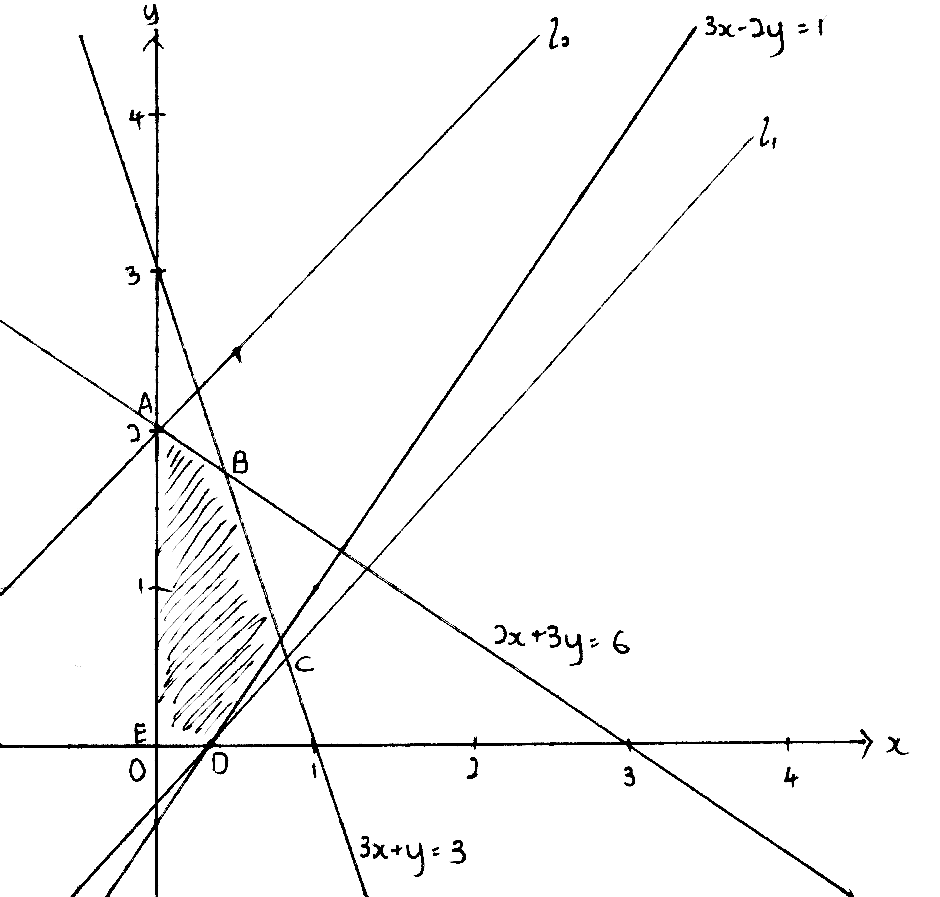
\includegraphics[scale=0.5]{g1}
              \end{center}
              When $y = x - z$ translates towards bottom right of the feasible region, the value of $z$ increases. Therefore, the maximum value of the objective function is the value of $z$ in $l_1$. The point of intersection $D$ of $l_1$ and the feasible region makes the objective function to have its maximum value. Since $D$ is also the point of intersection of $3x - 2y = 1$ and $y = 0$,
              \begin{flalign*}
                   & \begin{cases}
                         3x - 2y = 1 \\
                         y = 0
                     \end{cases}                             \\
                   & D = \left(\frac{1}{3}, 0\right)          \\
                   & z_{\max} = \frac{1}{3} - 0 = \frac{1}{3}\end{flalign*}
              When $y = x - z$ translates towards top left of the feasible region, the value of $z$ decreases. Therefore, the minimum value of the objective function is the value of $z$ in $l_2$. The point of intersection $A$ of $l_2$ and the feasible region makes the objective function to have its minimum the point of intersection of $2x + 3y = 6$ and $x = 0$,
              \begin{flalign*}
                   & \begin{cases}
                         2x + 3y = 6 \\
                         x = 0
                     \end{cases}          \\
                   & A = (0, 2)            \\
                   & z_{\min} = 0 - 2 = -2
              \end{flalign*}

        \item A factory produces two types of products: $A$ and $B$. The ingredients used in
              each kilogram of these two products are as follows:

              \begin{center}
                  \begin{tabular}{|c|c|c|}
                      \hline
                      \textbf{Product (per kg)} & \textbf{Ingr. X (kg)} & \textbf{Ingr. Y (kg)} \\
                      \hline
                      $A$                       & $0.6$                 & $0.5$                 \\
                      $B$                       & $0.3$                 & $0.7$                 \\
                      \hline
                  \end{tabular}
              \end{center}

              The profit of each kilogram of product $A$ and $B$ is $\$3$ and $\$5$
              respectively. The factory has $24kg$ of ingredient $X$ and $28kg$ of ingredient
              $Y$. How many kilograms of each product should be produced to maximize the
              profit?

              \sol{}

              Let $x$ be the number of kilograms of product $A$ and $y$ be the number of
              kilograms of product $B$.

              The objective function is $z = 3x + 5y$, which is the profit of the factory.
              According to the given information, we find the maximum of it.

              \begin{flalign*}
                  \begin{cases}
                      0.6x + 0.3y \leq 24 \\
                      0.5x + 0.7y \leq 28 \\
                      x \geq 0            \\
                      y \geq 0
                  \end{cases}
              \end{flalign*}

              After simplifying, we get:

              \begin{flalign*}
                  \begin{cases}
                      2x + y \leq 80   \\
                      5x + 7y \leq 280 \\
                      x \geq 0         \\
                      y \geq 0
                  \end{cases}
              \end{flalign*}

              The feasible region is as follows:

              \begin{center}
                  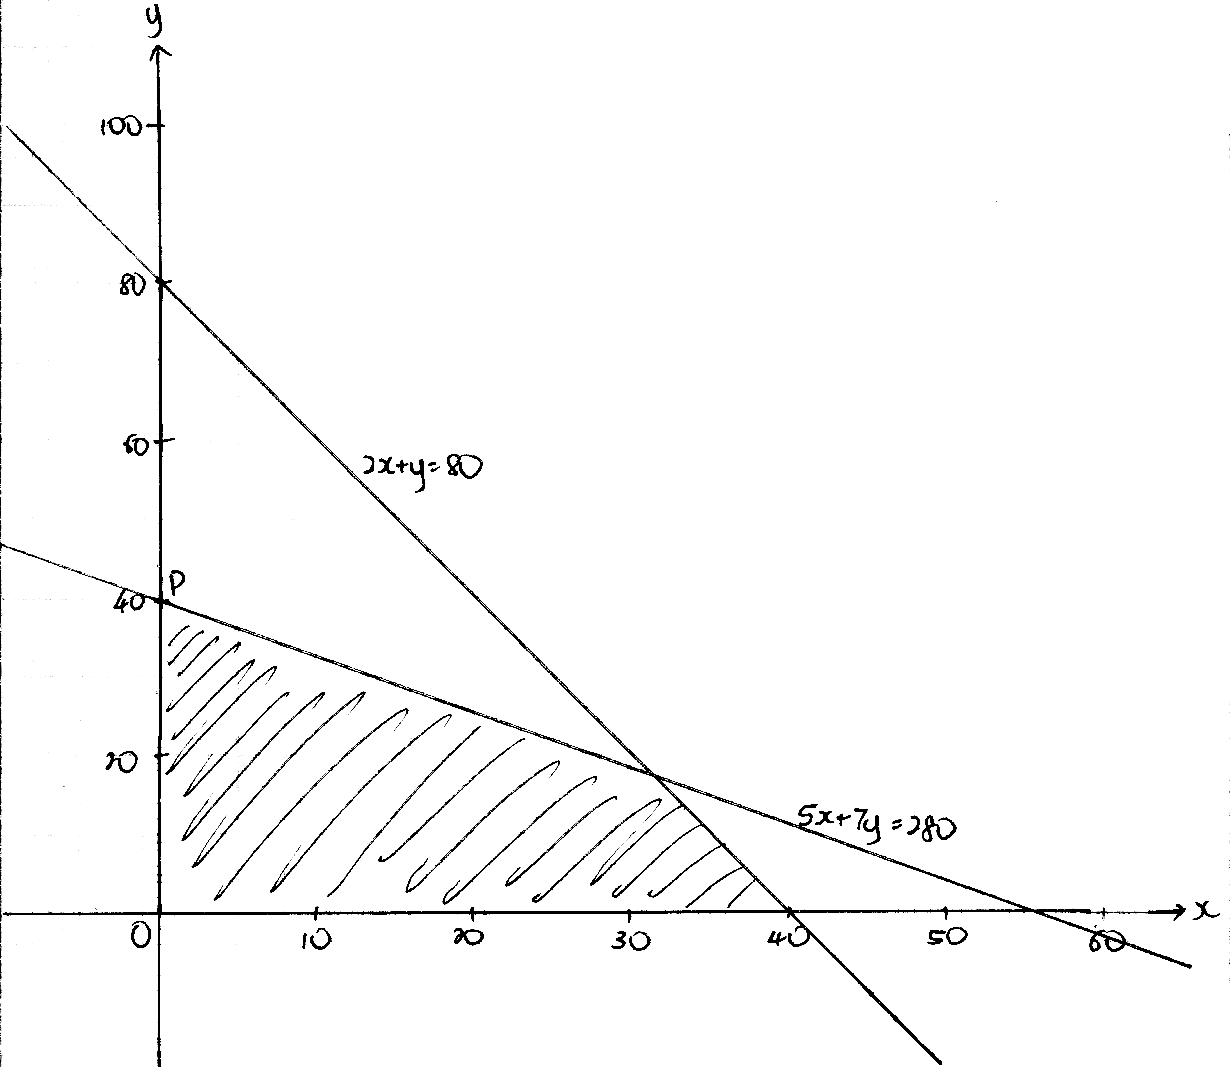
\includegraphics[scale=0.5]{g11}
              \end{center}

              When the line is at $l$, the value of $z$ is at its maximum. The point of
              intersection $P$ of $l$ and the feasible region makes the objective function to
              have its maximum value. Since $P$ is also the point of intersection of $5x + 7y
                  = 280$ and $x = 0$,

              \begin{flalign*}
                   & \begin{cases}
                         5x + 7y = 280 \\
                         x = 0
                     \end{cases} \\
                   & P = (0, 40)
              \end{flalign*}

              Thus, only $40kg$ of product $B$ should be produced to maximize the profit.

        \item An animal must consume three different kind of nutrients: $X$, $Y$ and $Z$ at
              least $11 units$, $13 units$ and $15 units$ respectively every day. There are
              two types of animal food: $A$ and $B$ that contain the following nutrients:

              \begin{center}
                  \begin{tabular}{|c|c|c|c|}
                      \hline
                      \textbf{Food} & \textbf{X (unit)} & \textbf{Y (unit)} & \textbf{Z (unit)} \\
                      \hline
                      $A$           & $1$               & $3$               & $2$               \\
                      $B$           & $2$               & $1$               & $2$               \\
                      \hline
                  \end{tabular}
              \end{center}

              The animal food $A$ costs $\$300$ per kilogram and the animal food $B$ costs
              $\$400$ per kilogram. How many kilograms of each food should be consumed to
              meet the daily nutrient requirement at the minimum cost? Find the minimum cost.

              \sol{}

              Let $x$ be the number of kilograms of food $A$ and $y$ be the number of
              kilograms of animal food $B$.

              The objective function is $z = 300x + 400y$, which is the cost of the food.
              According to the given information, we find the minimum of it. The constraints
              are:

              \begin{flalign*}
                  \begin{cases}
                      x + 2y \geq 11  \\
                      3x + y \geq 13  \\
                      2x + 2y \geq 15 \\
                      x \geq 0        \\
                      y \geq 0
                  \end{cases}
              \end{flalign*}

              The feasible region is as follows:

              \begin{center}
                  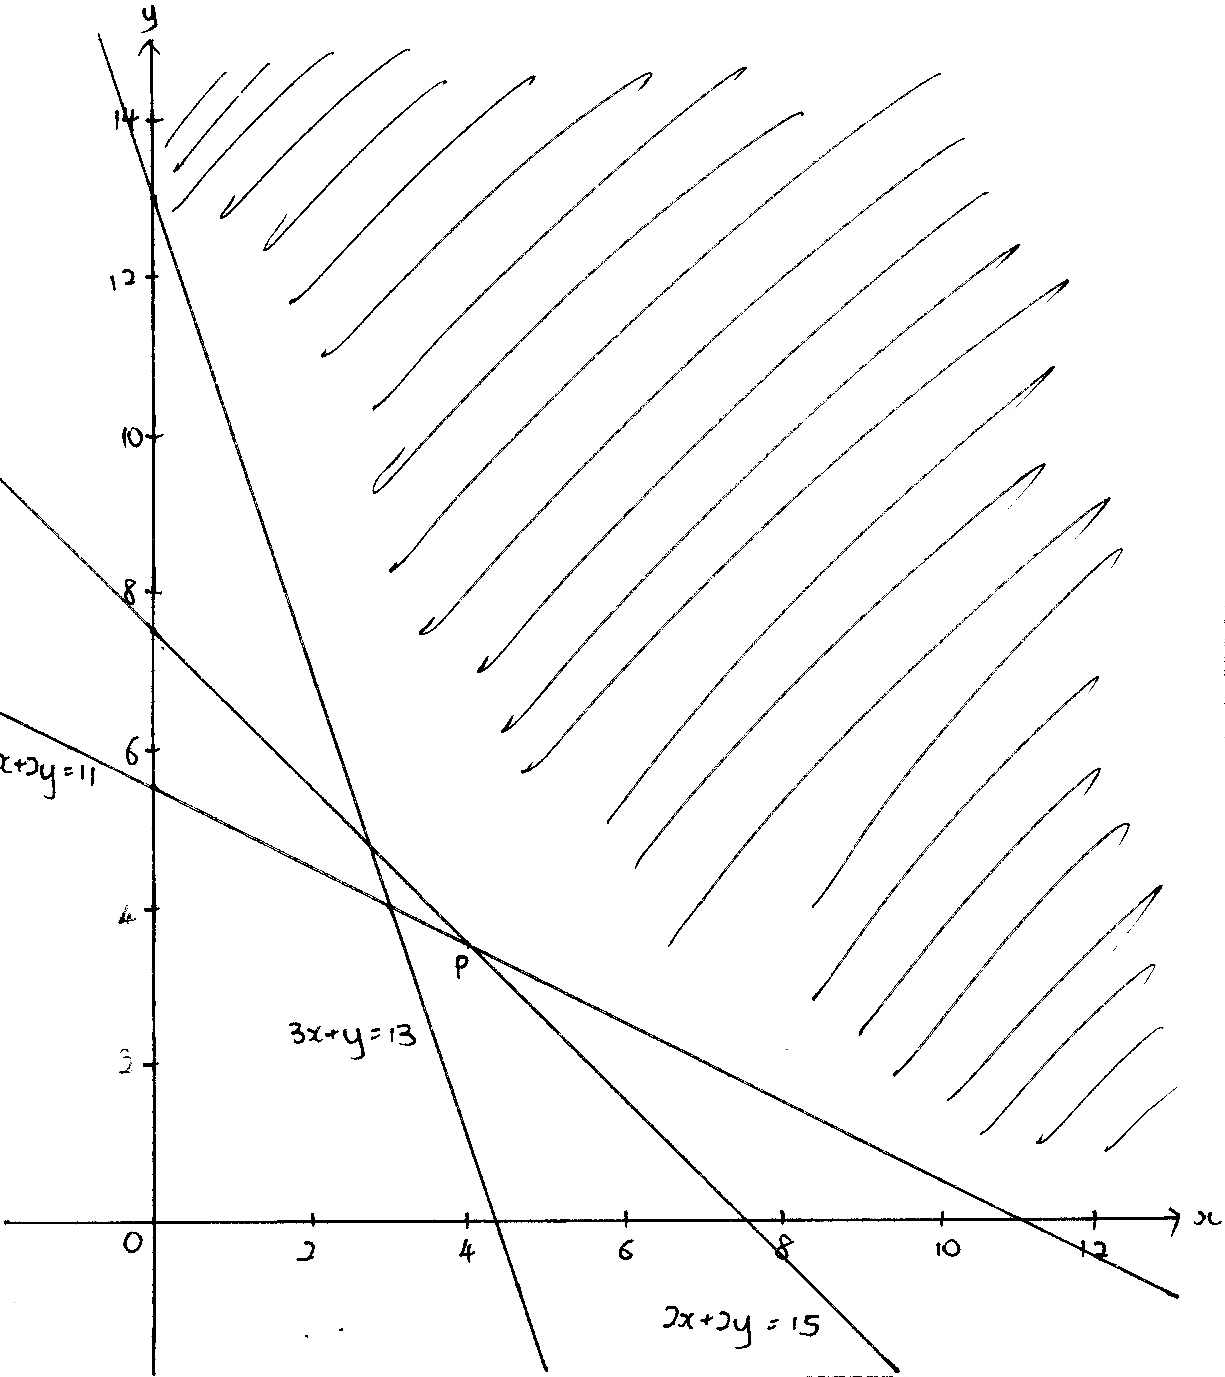
\includegraphics[scale=0.5]{g12}
              \end{center}

              When the line is at $l$, the value of $z$ is at its minimum. The point of
              intersection $P$ of $l$ and the feasible region makes the objective function to
              have its minimum value. Since $P$ is also the point of intersection of $x + 2y
                  = 11$ and $2x+2y = 15$,

              \setcounter{equation}{0}
              \begin{numcases}{}
                  x + 2y = 11 \\
                  2x + 2y = 15
              \end{numcases}

              \begin{flalign*}
                  (1):                               & \ 2y = 11 - x                                 \\
                  \text{Sub } (1) \text{ into } (2): & \ 2x + 11 - x = 15                            \\
                                                     & \ \ \ \ \ \ \ \ \ \ \ \ \ \ \ \ \ \ \ x = 4   \\
                                                     & \ \ \ \ \ \ \ \ \ \ \ \ \ \ \ \ \ \ \ y = 3.5 \\
                  \\
                  P                                  & = (4, 3.5)                                    \\
                  z_{\min}                           & = 300(4) + 400(3.5) = 2,600
              \end{flalign*}

              Thus, $4kg$ of food $A$ and $3.5kg$ of food $B$ should be consumed to meet the
              daily nutrient requirement at a minimum cost of $\$2,600$.
    \end{enumerate}

    \chapter{Circle}

      \section{Standard Equation of a Circle}

      The circle is a locus of points in a plane that are equidistant from a fixed
      point called the centre of the circle. The length from the centre to the points
      on the circle is called the radius of the circle.

      \begin{center}
            \begin{tikzpicture}
                  \draw[->] (-1,0) -- (5,0) node[right] {$x$};
                  \draw[->] (0,-1) -- (0,5) node[above] {$y$};
                  \draw (2,2) circle (1.5);
                  \filldraw[black] (2,2) circle (0.05);
                  \draw[black] (2,1.9) node[below] {\footnotesize$C(h,k)$};
                  \filldraw[black] (3.061, 3.061) circle (0.05);
                  \draw[black] (2.9, 2.9) node[above right] {\footnotesize$P(x,y)$};
                  \draw[black, densely dashed] (2,2) -- (3.061, 3.061);
                  \draw[black] (0,0) node[below left] {\footnotesize$O$};
            \end{tikzpicture}
      \end{center}

      The standard equation of a circle is given by
      \begin{cequation}
            (x-h)^2+{(y-k)}^2=r^2
      \end{cequation}
      where $(h,k)$ is the centre of the circle and $r$ is the radius of the circle.

      If the centre of the circle is at the origin, then the equation of the circle
      is
      \begin{cequation}
            x^2+y^2=r^2\ \ \ \ \ (r>0)
      \end{cequation}

      \subsection{Practice 1}

      \begin{enumerate}
            \item Find the equation of the circle with centre $(3, -1)$ and radius $2$. \sol{}
                  \begin{flalign*}
                        \text{Equation}: {(x-3)}^2+{[y+(-1)]}^2 & =2^2 \\
                        {(x-3)}^2+{(y+1)}^2                     & =4
                  \end{flalign*}

            \item Find the equation of the circle with centre $(-2, 9)$ and passing through the
                  point $(1, 5)$. \sol{}
                  \begin{flalign*}
                        r & = \sqrt{{(1-(-2))}^2+{(5-9)}^2} \\
                          & = \sqrt{9+16}                   \\
                          & = \sqrt{25}                     \\
                          & = 5
                  \end{flalign*}
                  \begin{flalign*}
                        \therefore\ \text{Equation}: {[x-(-2)]}^2+{(y-9)}^2 & =5^2 \\
                        {(x+2)}^2+{(y-9)}^2                                 & =25
                  \end{flalign*}
      \end{enumerate}

      \subsection{Exercise 16.1}

      \begin{enumerate}
            \item Find the equation of the circle with centre at the origin and radius $7$.
                  \sol{}
                  \begin{flalign*}
                        \text{Equation}: x^2+y^2 & =7^2 \\
                        x^2+y^2                  & =49  \\
                  \end{flalign*}

            \item Find the equation of circle of each of the following description:
                  \begin{enumerate}
                        \item Passing through the points $(5, -3)$ and centre at $(2, 1)$. \sol{}
                              \begin{flalign*}
                                    r & = \sqrt{{(5-2)}^2+{(-3-1)}^2} \\
                                      & = \sqrt{9+16}                 \\
                                      & = \sqrt{25}                   \\
                                      & = 5
                              \end{flalign*}
                              \begin{flalign*}
                                    \therefore\ \text{Equation}: {(x-2)}^2+{(y-1)}^2 & =5^2 \\
                                    {(x-2)}^2+{(y-1)}^2                              & =25
                              \end{flalign*}

                        \item Centre at $(3, 2)$ and radius $4$. \sol{}
                              \begin{flalign*}
                                    \text{Equation}: {(x-3)}^2+{(y-2)}^2 & =4^2 \\
                                    {(x-3)}^2+{(y-2)}^2                  & =16
                              \end{flalign*}
                        \item Centre at $(a, b)$ and radius $a+b$. \sol{}
                              \begin{flalign*}
                                    \text{Equation}: {(x-a)}^2+{(y-b)}^2 & ={(a+b)}^2 \\
                              \end{flalign*}
                  \end{enumerate}
            \item Given that the coordinates of two points on the end of the diameter of a circle
                  are $(5, -3)$ and $(3, 1)$, find the equation of the circle. \sol{}
                  \begin{flalign*}
                        C & = \left(\frac{5+3}{2}, \frac{-3+1}{2}\right) \\
                          & = \left(\frac{8}{2}, \frac{-2}{2}\right)     \\
                          & = \left(4, -1\right)                         \\
                        \\
                        r & = \sqrt{{(5-4)}^2+{(-3-(-1))}^2}             \\
                          & = \sqrt{1+4}                                 \\
                          & = \sqrt{5}
                  \end{flalign*}
                  \begin{flalign*}
                        \therefore\ \text{Equation}: {(x-4)}^2+{[y-(-1)]}^2 & = {(\sqrt{5})}^2 \\
                        {(x-4)}^2+{(y+1)}^2                                 & =5
                  \end{flalign*}
            \item Find the equation of the circle with a diameter connected by the points $(-3,
                        4)$ and $(9, 2)$. \sol{}
                  \begin{flalign*}
                        C & = \left(\frac{-3+9}{2}, \frac{4+2}{2}\right) \\
                          & = \left(\frac{6}{2}, \frac{6}{2}\right)      \\
                          & = \left(3, 3\right)                          \\
                        \\
                        r & = \sqrt{{(-3-3)}^2+{(4-3)}^2}                \\
                          & = \sqrt{36+1}                                \\
                          & = \sqrt{37}
                  \end{flalign*}
                  \begin{flalign*}
                        \therefore\ \text{Equation}: {(x-3)}^2+{(y-3)}^2 & = {(\sqrt{37})}^2 \\
                        {(x-3)}^2+{(y-3)}^2                              & =37
                  \end{flalign*}
            \item Given two points $P(-2, 2)$ and $Q(4, 6)$, find the equation of the circle wuth
                  line $PQ$ as its diameter. \sol{}
                  \begin{flalign*}
                        C & = \left(\frac{-2+4}{2}, \frac{2+6}{2}\right) \\
                          & = \left(\frac{2}{2}, \frac{8}{2}\right)      \\
                          & = \left(1, 4\right)                          \\
                        \\
                        r & = \sqrt{{(-2-1)}^2+{(2-4)}^2}                \\
                          & = \sqrt{9+4}                                 \\
                          & = \sqrt{13}
                  \end{flalign*}
                  \begin{flalign*}
                        \therefore\ \text{Equation}: {(x-1)}^2+{(y-4)}^2 & = {(\sqrt{13})}^2 \\
                        {(x-1)}^2+{(y-4)}^2                              & =13
                  \end{flalign*}
            \item Turn the equation $x^2+y^2-6x+12y+41=0$ into the standard form, and find the
                  centre and radius of the circle. \sol{}
                  \begin{flalign*}
                        x^2 + y^2 - 6x + 12y + 41                  & = 0   & \\
                        x^2 + y^2 - 6x + 12y                       & = -41 & \\
                        (x^2 - 6x + 9) - 9 + (y^2 + 12y + 36) - 36 & = -41 & \\
                        {(x-3)}^2 + {(y-6)}^2                      & = 4   &
                  \end{flalign*}
                  \begin{flalign*}
                        \therefore\ \text{Centre}: (3, 6),\ \text{Radius}: 2
                  \end{flalign*}
      \end{enumerate}

      \section{General Equation of a Circle}

      Expand the standard equation of a circle, we get
      \begin{cequation}
            x^2+y^2 -2hx-2ky+h^2+k^2-r^2=0
      \end{cequation}
      \setlength{\belowdisplayskip}{0pt} \setlength{\belowdisplayshortskip}{0pt}
      \setlength{\abovedisplayskip}{0pt} \setlength{\abovedisplayshortskip}{0pt}
      Let $g=-h$, $f=-k$, $c=h^2+k^2-r^2$, we get the general equation of a circle
      \begin{cequation}
            x^2+y^2+2gx+2fy+c=0
      \end{cequation}
      \begin{flalign*}
            \text{From }c=h^2+k^2-r^2\text{, we have }r^2 & =h^2+k^2-c                  & \\
            r                                             & =\sqrt{h^2+k^2-c}           & \\
                                                          & =\sqrt{{(-g)}^2+{(-f)}^2-c} & \\
                                                          & =\sqrt{g^2+f^2-c}
      \end{flalign*}
      \setlength{\belowdisplayskip}{10pt} \setlength{\belowdisplayshortskip}{10pt}
      \setlength{\abovedisplayskip}{10pt} \setlength{\abovedisplayshortskip}{10pt}
      \noindent Thus,
      \begin{enumerate}
            \item When $g^2+f^2-c>0$, the image is a real circle with centre $(g,f)$ and radius
                  $\sqrt{g^2+f^2-c}$.
            \item When $g^2+f^2-c=0$, the image is point $(g,f)$.
            \item When $g^2+f^2-c<0$, the image does not exist.
      \end{enumerate}

      \subsection{Practice 2}

      \begin{enumerate}
            \item Find the centre and radius of the circle with equation $x^2+y^2-6x-8y+21=0$.
                  \sol{}
                  \begin{flalign*}
                        x^2+y^2-6x-8y+21                  & =0   \\
                        \therefore\ 2g = -6,\ 2f = -8,\ c & = 21 \\
                        g = -3,\ f = -4,\ c               & = 21
                  \end{flalign*}
                  \begin{flalign*}
                        \therefore\ C & = (3, 4)                      \\
                        r             & = \sqrt{{(-3)}^2+{(-4)}^2-21} \\
                                      & = \sqrt{9+16-21}              \\
                                      & = \sqrt{4}                    \\
                                      & = 2
                  \end{flalign*}
            \item Find the equaton of the circle that passes through the following points:
                  \begin{enumerate}
                        \item $A(0, 0)$, $B(2, 0)$, $C(0, -3)$.
                              \sol{}

                              Let the equation of the circle be $x^2+y^2+2gx+2fy+c=0$,
                              \begin{flalign*}
                                     & \begin{cases}
                                             0 + 0 + 0g + 0f + c = 0 \\
                                             4 + 0 + 4g + 0f + c = 0 \\
                                             0 + 9 + 0g -6f + c = 0
                                       \end{cases} \\
                                     & \begin{cases}
                                             c = 0          \\
                                             4 + 4g + c = 0 \\
                                             9 - 6f + c = 0
                                       \end{cases}          \\
                                     & \begin{cases}
                                             c = 0      \\
                                             4 + 4g = 0 \\
                                             9 - 6f = 0
                                       \end{cases}              \\
                                     & \begin{cases}
                                             c = 0   \\
                                             4g = -4 \\
                                             -6f = -9
                                       \end{cases}                 \\
                                     & \begin{cases}
                                             c = 0  \\
                                             g = -1 \\
                                             f = \frac{3}{2}
                                       \end{cases}
                              \end{flalign*}
                              \begin{flalign*}
                                    \therefore\ \text{Equation}: x^2+y^2+2(-1)+2(\frac{3}{2}) + 0 & =0 & \\
                                    x^2+y^2-2+3                                                   & =0 & \\
                                    x^2+y^2+1                                                     & =0 &
                              \end{flalign*}
                        \item $K(0, 3)$, $L(1, 2)$, $M(2, -1)$.
                              \sol{}

                              Let the equation of the circle be $x^2+y^2+2gx+2fy+c=0$,
                              \begin{flalign*}
                                     & \begin{cases}
                                             0 + 9 + 0g + 6f + c = 0 \\
                                             1 + 4 + 2g + 4f + c = 0 \\
                                             4 + 1 + 4g -2f + c = 0
                                       \end{cases} \\
                                     & \begin{cases}
                                             6f + c = -9      \\
                                             2g + 4f + c = -5 \\
                                             4g - 2f + c = -5
                                       \end{cases}
                              \end{flalign*}
                              \begin{flalign*}
                                    g = 3,\ f = 1,\ c = -15
                              \end{flalign*}
                              \begin{flalign*}
                                    \therefore\ \text{Eq.}: x^2+y^2+2(3)x+2(1)y + (-15) & =0 & \\
                                    x^2+y^2+6x+2y-15                                    & =0 &
                              \end{flalign*}
                  \end{enumerate}
            \item Given that the vertices of $\Delta ABC$ are $(1, 2)$, $(2, 5)$ and $(-1, 2)$,
                  find the equation of the circumcircle of $\Delta ABC$. \sol{}

                  Let the equation of the circumcircle be $x^2+y^2+2gx+2fy+c=0$,
                  \begin{flalign*}
                         & \begin{cases}
                                 1 + 4 + 2g + 4f + c = 0   \\
                                 4 + 25 + 8g + 10f + c = 0 \\
                                 1 + 4 - 2g + 4f + c = 0
                           \end{cases} \\
                         & \begin{cases}
                                 2g + 4f + c = -5   \\
                                 8g + 10f + c = -29 \\
                                 -2g + 4f + c = -5
                           \end{cases}
                  \end{flalign*}
                  \begin{flalign*}
                        g = 0,\ f = -4,\ c = 11
                  \end{flalign*}
                  \begin{flalign*}
                        \therefore\ \text{Eq.}: x^2+y^2+2(0)x+2(-4)y + 11 & =0 & \\
                        x^2+y^2-8y+11                                     & =0 &
                  \end{flalign*}
      \end{enumerate}

      \subsection{Exercise 16.2}

      \begin{enumerate}
            \item Find the centre and radius of the circle with the following equation:
                  \begin{enumerate}
                        \item $x^2+y^2-64=0$
                              \sol{}
                              \begin{flalign*}
                                    x^2+y^2-64          & =0    \\
                                    2g = 0,\ 2f = 0,\ c & = -64 \\
                                    g = 0,\ f = 0,\ c   & = -64 \\
                              \end{flalign*}
                              \begin{flalign*}
                                    \therefore\ C & = (0, 0)               \\
                                    r             & = \sqrt{0^2+0^2-(-64)} \\
                                                  & = 8
                              \end{flalign*}

                        \item $x^2+y^2-4x-8y=44$
                              \sol{}
                              \begin{flalign*}
                                    x^2+y^2-4x-8y         & =44   \\
                                    x^2+y^2-4x-8y-44      & =0    \\
                                    2g = -4,\ 2f = -8,\ c & = -44 \\
                                    g = -2,\ f = -4,\ c   & = -44 \\
                              \end{flalign*}
                              \begin{flalign*}
                                    \therefore\ C & = (2, 4)                         \\
                                    r             & = \sqrt{{(-2)}^2+{(-4)}^2-(-44)} \\
                                                  & = \sqrt{4 + 16 + 44}             \\
                                                  & = \sqrt{64}                      \\
                                                  & = 8
                              \end{flalign*}

                        \item $x^2+y^2-8x=0$
                              \sol{}
                              \begin{flalign*}
                                    x^2+y^2-8x           & =0  \\
                                    2g = -8,\ 2f = 0,\ c & = 0 \\
                                    g = -4,\ f = 0,\ c   & = 0 \\
                              \end{flalign*}
                              \begin{flalign*}
                                    \therefore\ C & = (4, 0)                    \\
                                    r             & = \sqrt{{(-4)}^2+{0}^2-{0}} \\
                                                  & = 4
                              \end{flalign*}

                        \item $9x^2+9y^2+2x-6y-6=0$
                              \sol{}
                              \begin{flalign*}
                                    9x^2+9y^2+2x-6y-6                             & =0             \\
                                    x^2+y^2+\frac{2}{9}x-\frac{2}{3}y-\frac{2}{3} & =0             \\
                                    2g = \frac{2}{9},\ 2f = -\frac{2}{3},\ c      & = -\frac{2}{3} \\
                                    g = \frac{1}{9},\ f = -\frac{1}{3},\ c        & = -\frac{2}{3} \\
                              \end{flalign*}
                              \begin{flalign*}
                                    \therefore\ C & = \left(-\frac{1}{9}, \frac{1}{3}\right)                                                          \\
                                    r             & = \sqrt{{\left(\frac{1}{9}\right)}^2 + {\left(-\frac{1}{3}\right)}^2 - \left(-\frac{2}{3}\right)} \\
                                                  & = \sqrt{\frac{64}{81}}                                                                            \\
                                                  & = \frac{8}{9}
                              \end{flalign*}
                  \end{enumerate}

            \item Find the equation of the circle that passes through the following points:
                  \begin{enumerate}
                        \item $A(1, 1)$, $B(1, -1)$, $C(-2, 1)$
                              \sol{}
                              Let the equation of the circle be $x^2+y^2+2gx+2fy+c=0$,
                              \begin{flalign*}
                                     & \begin{cases}
                                             1 + 1 + 2g + 2f + c = 0 \\
                                             1 + 1 + 2g - 2f + c = 0 \\
                                             4 + 1 - 4g + 2f + c = 0
                                       \end{cases} \\
                                     & \begin{cases}
                                             2g + 2f + c = -2 \\
                                             2g - 2f + c = -2 \\
                                             -4g + 2f + c = -5
                                       \end{cases}
                              \end{flalign*}
                              \begin{flalign*}
                                    g = \frac{1}{2},\ f = 0,\ c & = -3
                              \end{flalign*}
                              \begin{flalign*}
                                    \therefore\ \text{Eq} : x^2+y^2+2\left(\frac{1}{2}\right)x+2(0)y+(-3) & =0 & \\
                                    x^2+y^2+x-3                                                           & =0 & \\
                              \end{flalign*}

                        \item $F(0, 0)$, $G(3, -3)$, $H(-1, 0)$
                              \sol{}
                              Let the equation of the circle be $x^2+y^2+2gx+2fy+c=0$,
                              \begin{flalign*}
                                     & \begin{cases}
                                             0 + 0 + 0g + 0f + c = 0 \\
                                             9 + 9 + 6g - 6f + c = 0 \\
                                             1 + 0 - 2g + 0f + c = 0
                                       \end{cases} \\
                                     & \begin{cases}
                                             c = 0         \\
                                             6g - 6f = -18 \\
                                             -2g = -1
                                       \end{cases}           \\
                                     & \begin{cases}
                                             c = 0      \\
                                             g - f = -3 \\
                                             g = \frac{1}{2}
                                       \end{cases}              \\
                                     & \begin{cases}
                                             c = 0           \\
                                             f = \frac{7}{2} \\
                                             g = \frac{1}{2}
                                       \end{cases}
                              \end{flalign*}
                              \begin{flalign*}
                                    \therefore\ \text{Eq} : x^2+y^2+2\left(\frac{1}{2}\right)x+2\left(\frac{7}{2}\right)y+0 & =0 & \\
                                    x^2+y^2+x+7y                                                                            & =0 &
                              \end{flalign*}

                        \item $P(1, 0)$, $Q(0, -3)$, $R(3, 4)$
                              \sol{}
                              Let the equation of the circle be $x^2+y^2+2gx+2fy+c=0$,
                              \begin{flalign*}
                                     & \begin{cases}
                                             1 + 0 + 2g + 0f + c = 0 \\
                                             0 + 9 + 0g - 6f + c = 0 \\
                                             9 + 16 + 6g + 8f + c = 0
                                       \end{cases} \\
                                     & \begin{cases}
                                             2g + c = -1  \\
                                             -6f + c = -9 \\
                                             6g + 8f + c = -25
                                       \end{cases}
                              \end{flalign*}
                              \begin{flalign*}
                                    g = -26,\ f = 10,\ c = 51
                              \end{flalign*}
                              \begin{flalign*}
                                    \therefore\ \text{Eq} : x^2+y^2+2(-26)x+2(10)y+51 & =0 & \\
                                    x^2+y^2-52x+20y+51                                & =0 &
                              \end{flalign*}
                  \end{enumerate}
            \item A circle passes through point $A(2, 2)$ and $B(5, 3)$ while intersecting the
                  line $x+y=4$ at y-axis. Find the equation of the circle. \sol{}
                  \begin{flalign*}
                        x + y                              & = 4     \\
                        \text{When } x = 0, \ y            & = 4     \\
                        \therefore\ \text{Another point: } & C(0, 4)
                  \end{flalign*}
                  Let the equation of the circle be $x^2+y^2+2gx+2fy+c=0$,
                  \begin{flalign*}
                         & \begin{cases}
                                 4 + 4 + 4g + 4f + c = 0   \\
                                 25 + 9 + 10g + 6f + c = 0 \\
                                 0 + 16 + 0g + 8f + c = 0
                           \end{cases} \\
                         & \begin{cases}
                                 4g + 4f + c = -8   \\
                                 10g + 6f + c = -34 \\
                                 8f + c = -16
                           \end{cases}
                  \end{flalign*}
                  \begin{flalign*}
                        g = -\frac{11}{4},\ f = -\frac{19}{4}, c = 22
                  \end{flalign*}
                  \begin{flalign*}
                        \therefore\ \text{Eq} : x^2+y^2+2\left(-\frac{11}{4}\right)x+2\left(-\frac{19}{4}\right)y+22 & =0 & \\
                        x^2+y^2-\frac{11}{2}x-\frac{19}{2}y+22                                                       & =0 &
                  \end{flalign*}
      \end{enumerate}

      \section{Problems Related to Circles}

      \subsection*{Tangent to a Circle}

      When a straight line $l$ and a circle intersect at a point $P$, the line $l$ is
      called a tangent to the circle, and the point $P$ is called the point of
      contact. The tangent line is perpendicular to the radius at the point of
      contact. That is to say, when the length from the point of tangency to the
      centre of the circle is equal to the radius of the circle, the line is a
      tangent to the circle.

      \begin{center}
            \begin{tikzpicture}
                  % draw a circle and its tangent 
                  \draw (0, 0) circle (2);
                  \draw (2.828, 0) -- (0, -2.828);
                  \node at (2.828, 0) [above right] {$l$};
                  \filldraw (0, 0) circle (0.05);
                  \node at (0, 0) [above left] {$O$};
                  \draw (0, 0) -- (1.4142, -1.4142);
                  \filldraw (1.4142, -1.4142) circle (0.05);
                  \node at (1.4142, -1.4142) [below right] {$P$};
                  \node (A) at (0.74, -2.088) {};
                  \node (B) at (2.35, -0.478) {};
                  \node (P) at (0.84, -0.84) {};
                  \draw [black,right angle symbol={A}{B}{P}];

            \end{tikzpicture}
      \end{center}

      \subsection*{Length of a Tangent}

      According to the theorem of length of tangent, the lengths of tangents drawn
      from an external point to a circle are equal.

      \begin{center}
            \begin{tikzpicture}
                  % draw a circle and its tangent 
                  \draw (0, 0) circle (2);
                  \draw (-1, -2.736) -- (4.472, 0);
                  \draw (-1, 2.736) -- (4.472, 0);
                  \filldraw (0.8894, 1.7889) circle (0.05);
                  \node at (0.8894, 1.7889) [above] {$A$};
                  \filldraw (0.8894, -1.7889) circle (0.05);
                  \node at (0.8894, -1.7889) [below] {$B$};
                  \filldraw (0, 0) circle (0.05);
                  \node at (0, 0) [left] {$C$};
                  \filldraw (4.472, 0) circle (0.05);
                  \node at (4.472, 0) [right] {$P$};
                  \draw [dashed] (0, 0) -- (4.472, 0);
                  \draw [dashed] (0, 0) -- (0.8894, 1.7889);
                  \node (A) at (0, 2.236) {};
                  \node (B) at (4.472, 0) {};
                  \node (P) at (0, 0) {};
                  \draw [black,right angle symbol={A}{B}{P}];
            \end{tikzpicture}
      \end{center}

      Let the equation of the circle be $x^2+y^2+2gx+2fy+c=0$, the external point P
      be $(x_1, y_1)$. Connect $PC$ and $CA$, $\angle CPA=90^{\circ}$, the coordinate
      of centre of the circle $C$ be $(-g, -f)$.
      \begin{flalign*}
            \therefore\ CA = \sqrt{g^2+f^2 - c},\ PC = \sqrt{{(x_1+g)}^2+{(y_1+f)}^2}
      \end{flalign*}
      \noindent From the Pythagorean theorem,
      \begin{flalign*}
            {PA}^2 & = PC^2 - CA^2                             \\
                   & = {(x_1+g)}^2+{(y_1+f)}^2 - (g^2+f^2 - c) \\
                   & = x_1^2 + y_1^2 + 2gx_1 + 2fy_1 + c
      \end{flalign*}
      Thus, the length of the tangent is given by
      \begin{flalign*}
            PA = \sqrt{x_1^2 + y_1^2 + 2gx_1 + 2fy_1 + c}
      \end{flalign*}
      Note that the coefficient of $x_1$ and $y_1$ in the above equation must be 1.
      \subsection*{Maximum and Minimum Distance of a Point from a Circle}

      Given a circle with centre $C$ and radius $r$ and a point $P$ anywhere on the
      plane,

      When $PC > r$, point $P$ is said to be outside the circle, the maximum distance
      of $P$ from the circle is $M = PC + r$, and the minimum distance of $P$ from
      the circle is $m = PC - r$.
      \begin{center}
            \begin{tikzpicture}
                  % draw a circle 
                  \draw (0, 0) circle (2);
                  \filldraw (0, 0) circle (0.05);
                  \node at (0, 0) [below] {$C$};
                  \filldraw (2, 0) circle (0.05);
                  \node at (2, 0) [below left] {$R$};
                  \filldraw (3.5, 0) circle (0.05);
                  \node at (3.5, 0) [right] {$P$};
                  \filldraw (-2, 0) circle (0.05);
                  \node at (-2, 0) [left] {$Q$};
                  \draw [dashed] (0, 0) -- (-2, 0) node[pos=0.5,below,black]{$r$};
                  \draw (0, 0) -- (3.5, 0);
                  \draw [decorate, decoration = {calligraphic brace,amplitude=5pt}] (-2,0.2) --  (3.5,0.2) node[pos=0.5,above=5pt,black]{$M$};
                  \draw [decorate, decoration = {calligraphic brace, mirror, amplitude=5pt}] (2,-0.2) --  (3.5,-0.2) node[pos=0.5,below=5pt,black]{$m$};
            \end{tikzpicture}
      \end{center}

      When $PC < r$, point $P$ is said to be inside the circle, the maximum distance
      of $P$ from the circle is $M = PC + r$, and the minimum distance of $P$ from
      the circle is $m = r - PC$.
      \begin{center}
            \begin{tikzpicture}
                  % draw a circle 
                  \draw (0, 0) circle (2);
                  \filldraw (0, 0) circle (0.05);
                  \node at (0, 0) [below] {$C$};
                  \filldraw (2, 0) circle (0.05);
                  \node at (2, 0) [right] {$R$};
                  \filldraw (1, 0) circle (0.05);
                  \node at (1, 0) [above] {$P$};
                  \filldraw (-2, 0) circle (0.05);
                  \node at (-2, 0) [left] {$Q$};
                  \draw [dashed] (0, 0) -- (-2, 0) node[pos=0.5,below,black]{$r$};
                  \draw (0, 0) -- (2, 0);
                  \draw [decorate, decoration = {calligraphic brace,amplitude=5pt}] (-2,0.2) --  (1,0.2) node[pos=0.5,above=5pt,black]{$M$};
                  \draw [decorate, decoration = {calligraphic brace, mirror, amplitude=5pt}] (1,-0.2) --  (2,-0.2) node[pos=0.5,below=5pt,black]{$m$};
            \end{tikzpicture}
      \end{center}

      \subsection{Practice 3}

      \begin{enumerate}
            \item Find the euqaiton of the circle with centre $(3, 4)$ and is tangent to the line
                  $x + 2y - 6 = 0$. \sol{}
                  \begin{flalign*}
                        r & = \left|\frac{1(3) + 2(4) - 6}{\sqrt{1^2 + 2^2}}\right| \\
                          & = \left|\frac{3 + 8 - 6}{\sqrt{5}}\right|               \\
                          & = \left|\frac{5}{\sqrt{5}}\right|                       \\
                          & = \frac{5\sqrt{5}}{5}                                   \\
                          & = \sqrt{5}
                  \end{flalign*}
                  \begin{flalign*}
                        g = -3,\ f = -4,\ c & = {(-3)}^2 + {(-4)}^2 - {(\sqrt{5})}^2 \\
                                            & = 9 + 16 - 5                           \\
                                            & = 20
                  \end{flalign*}
                  \begin{flalign*}
                        \therefore\ \text{Eq}: x^2 + y^2 + 2(-3)x + 2(-4)y - 20 & = 0 \\
                        x^2 + y^2 - 6x - 8y - 20                                & = 0
                  \end{flalign*}

            \item A circle passes through the points $(2, -3)$ and $(-2, -5)$, and its centre is
                  on the line $x - 2y = 3$. Find the equation of the circle. \sol{}

                  Let the centre of the circle be $C(h, k)$, point (2, -3) be $A$ and point (-2,
                  -5) be $B$.
                  \begin{flalign*}
                        \because\ C \text{ is on the line } x - 2y & = 3                                  & \\
                        h - 2k                                     & = 3\ \ \ \ \ \ \ \ \ \  (1)          & \\
                        \\
                        CA                                         & = CB                                 & \\
                        \sqrt{{(2 - h)}^2 + {(-3 - k)}^2}          & = \sqrt{{(-2 - h)}^2 + {(-5 - k)}^2} & \\
                        h^2 - 4h + 4 + k^2                         & = h^2 + 4h + 4 + k^2                 & \\
                        + 6k + 9                                   & \ \ \ \ + 10k + 25                   & \\
                        -4h + 6k + 13                              & = 4h + 10k + 29                      & \\
                        -8h - 4k                                   & = 16                                 & \\
                        2h + k                                     & = -4\ \ \ \ \ \ \ \ \ \  (2)         & \\
                        \\
                        \text{Solving } (1) \text{ and } (2),\     & h = -1,\ k = -2
                  \end{flalign*}
                  \begin{flalign*}
                        \therefore\ C = (-1, -2) ,\        r & = \sqrt{{(2 - (-1))}^2 + {(-3 - (-2))}^2} & \\
                                                             & = \sqrt{3^2 + 1^2}                        & \\
                                                             & = \sqrt{10}                               & \\
                        g = 1,\ f = -2,\ c                   & = {(-1)}^2 + {(-2)}^2 - {(\sqrt{10})}^2   & \\
                                                             & = 1 + 4 - 10                              & \\
                                                             & = -5
                  \end{flalign*}
                  \begin{flalign*}
                        \therefore\ \text{Eq}: x^2 + y^2 + 2(-1)x + 2(-2)y - 5 & = 0 \\
                        x^2 + y^2 - 2x - 4y - 5                                & = 0
                  \end{flalign*}

            \item A circle with radius $\sqrt{5}$ are tangent with the line $x - 2y - 1 = 0$ at
                  the point $(3, 1)$. Find the equation of the circle. \sol{}

                  Let the centre of the circle be $C(h, k)$, point (3, 1) be $P$.
                  \begin{flalign*}
                        x - 2y - 1 & = 0                          \\
                        2y         & = x - 1                      \\
                        y          & = \frac{1}{2}x - \frac{1}{2} \\
                        m          & = \frac{1}{2}
                  \end{flalign*}
                  Let the line that passes through $P$ and is perpendicular to $x - 2y - 1 = 0$ be $l$.
                  \begin{flalign*}
                        m_l \times m & = -1        \\
                        m_l          & = -2        \\
                        l: y - 1     & = -2(x - 3) \\
                        y - 1        & = -2x + 6   \\
                        y            & = -2x + 7
                  \end{flalign*}
                  \begin{flalign*}
                        \because\ C(h, k) \text{ is on the line } l & \\
                        k = -2h + 7 \ \ \ \ \ \ \ \ \ \  (1)
                  \end{flalign*}
                  \begin{flalign*}
                        \sqrt{{(3 - h)}^2 + {(1 - k)}^2} & = \sqrt{5}                   \\
                        h^2 - 6h + 9 + k^2 - 2k + 1      & = 5 \ \ \ \ \ \ \ \ \ \  (2)
                  \end{flalign*}
                  \begin{flalign*}
                        \text{Sub } (1) \text{ in } (2),                                  &     \\
                        h^2 - 6h + 9 + {(-2h + 7)}^2 - 2(-2h + 7) + 1                     & = 5 \\
                        h^2 - 6h + 9 + 4h^2 - 28h + 49 + 4h - 14 + 1                      & = 5 \\
                        5h^2 - 30h + 40                                                   & = 0 \\
                        h^2 - 6h + 8                                                      & = 0 \\
                        (h-4)(h-2)                                                        & = 0 \\
                        h                                               = 4 \text{ or } h & = 2
                  \end{flalign*}
                  \begin{flalign*}
                        \text{Sub } h = 4 \text{ in } (1),\ k & = -2(4) + 7 = -1 \\
                        \text{Sub } h = 2 \text{ in } (1),\ k & = -2(2) + 7 = 3
                  \end{flalign*}
                  \begin{flalign*}
                        \therefore\ C = (4, -1) \text{ or } C = (2, 3)
                  \end{flalign*}
                  \begin{flalign*}
                        \text{When } C     & = (4, -1),                        \\
                        g = -4,\ f = 1,\ c & = 4^2 + {(-1)}^2 - {(\sqrt{5})}^2 \\
                                           & = 16 + 1 - 5                      \\
                                           & = 12
                  \end{flalign*}
                  \begin{flalign*}
                        \therefore\ \text{Eq}: x^2 + y^2 + 2(-4)x + 2(1)y + 12 & = 0 \\
                        x^2 + y^2 - 8x + 2y + 12                               & = 0
                  \end{flalign*}
                  \begin{flalign*}
                        \text{When } C      & = (2, 3),                    \\
                        g = -2,\ f = -3,\ c & = 2^2 + 3^2 - {(\sqrt{5})}^2 \\
                                            & = 4 + 9 - 5                  \\
                                            & = 8
                  \end{flalign*}
                  \begin{flalign*}
                        \therefore\ \text{Eq}: x^2 + y^2 + 2(-2)x + 2(-3)y + 8 & = 0 \\
                        x^2 + y^2 - 4x - 6y + 8                                & = 0
                  \end{flalign*}

            \item Prove the following lines are tangent to the following circles:
                  \begin{enumerate}
                        \item $3x - y - 5 = 0$, $x^2 + y^2 - 16x + 2y + 25 = 0$
                              \prooff{}
                              \begin{flalign*}
                                    C & = (8, -1)                                                     \\
                                    r & = \sqrt{{(-8)}^2 + 1^2 - 25} = 2\sqrt{10}                     \\
                                    d & = \left|\frac{3(8) - 1(-1) - 5}{\sqrt{3^2 + {(-1)}^2}}\right| \\
                                      & = \left|\frac{20}{\sqrt{10}}\right|                           \\
                                      & = \frac{20\sqrt{10}}{10}                                      \\
                                      & = 2\sqrt{10}
                              \end{flalign*}
                              \begin{flalign*}
                                    \because\    & d = r                                       \\
                                    \therefore\  & \text{The line} \ 3x - y - 5 = 0 \ \text{is
                                    tangent to}                                                \\
                                                 & \text{the circle} \ x^2 + y^2 - 16x + 2y +
                                    25 = 0
                              \end{flalign*}
                        \item $2x - y - 1 = 0$, $x^2 + y^2 + 2x - 4y = 0$
                              \prooff{}
                              \begin{flalign*}
                                    C & = (-1, 2)                                                     \\
                                    r & = \sqrt{1^2 + {(-2)}^2} = \sqrt{5}                            \\
                                    d & = \left|\frac{2(-1) - 1(2) - 1}{\sqrt{2^2 + {(-1)}^2}}\right| \\
                                      & = \left|\frac{-5}{\sqrt{5}}\right|                            \\
                                      & = \frac{5\sqrt{5}}{5}                                         \\
                                      & = \sqrt{5}
                              \end{flalign*}
                              \begin{flalign*}
                                    \because\    & d = r                                       \\
                                    \therefore\  & \text{The line} \ 2x - y - 1 = 0 \ \text{is
                                    tangent to}                                                \\
                                                 & \text{the circle} \ x^2 + y^2 + 2x - 4y = 0
                              \end{flalign*}
                  \end{enumerate}
            \item Find the length of the tangent from the point $P(8, 3)$ to the circle $x^2 +
                        y^2 - 8 = 0$. \sol{}
                  \begin{flalign*}
                        d = \sqrt{8^2 + 3^2 + 2(0)(8) + 2(0)(3) -8} = \sqrt{65}
                  \end{flalign*}
      \end{enumerate}

      \subsection{Exercise 16.3}

      \begin{enumerate}
            \item Find the equation of the circle that passes through the points $(1, 4)$ and
                  $(0, -3)$, and its centre is on the line $x - 2y = 4$. \sol{}

                  Let the centre of the circle be $C(h, k)$, point (1, 4) be $A$ and point (0,
                  -3) be $B$.
                  \begin{flalign*}
                        \because\ C \text{ is on the line } x - 2y & = 4                                 & \\
                        h - 2k                                     & = 4\ \ \ \ \ \ \ \ \ \  (1)         & \\
                        \\
                        CA                                         & = CB                                & \\
                        \sqrt{{(1 - h)}^2 + {(4 - k)}^2}           & = \sqrt{{(0 - h)}^2 + {(-3 - k)}^2} & \\
                        h^2 - 2h + 1 + k^2 - 8k + 16               & = h^2 + k^2+ 6k + 9                 & \\
                        -2h + -14k                                 & = -8                                & \\
                        h + 7k                                     & = 4\ \ \ \ \ \ \ \ \ \  (2)         & \\
                        \\
                        \text{Solving } (1) \text{ and } (2),\     & h = 4,\ k = 0
                  \end{flalign*}
                  \begin{flalign*}
                        \therefore\ C = (4, 0) ,\        r & = \sqrt{{(1 - 4)}^2 + {(4 - 0)}^2} & \\
                                                           & = \sqrt{{(-3)}^2 + 4^2}            & \\
                                                           & = \sqrt{25}                        & \\
                                                           & = 5                                & \\
                        g = -4,\ f = 0,\ c                 & = {(-4)}^2 + 0^2 - 5^2             & \\
                                                           & = 16 - 25                          & \\
                                                           & = -9
                  \end{flalign*}
                  \begin{flalign*}
                        \therefore\ \text{Eq}: x^2 + y^2 + 2(-4)x + 2(0)y - 9 & = 0 \\
                        x^2 + y^2 - 8x - 9                                    & = 0
                  \end{flalign*}

            \item Find the equation of the circle that passes through the points $(3, 2)$ and
                  $(-4, -5)$, and its centre is on the line $3x + y + 6 = 0$. \sol{}

                  Let the centre of the circle be $C(h, k)$, point (3, 2) be $A$ and point (-4,
                  -5) be $B$.
                  \begin{flalign*}
                        \because\ C \text{ is on the line } 3x + y + 6 & = 0                         & \\
                        3h + k + 6                                     & = 0\ \ \ \ \ \ \ \ \ \  (1)
                  \end{flalign*}
                  \begin{flalign*}
                        CA                                      & = CB                                 & \\
                        \sqrt{{(3 - h)}^2 + {(2 - k)}^2}        & = \sqrt{{(-4 - h)}^2 + {(-5 - k)}^2} & \\
                        h^2 - 6h + 9 + k^2                      & = h^2 + 8h + 16 + k^2                & \\
                        - 4k + 4                                & \ \ \ \ + 10k + 25                   & \\
                        -14h -14k                               & = 28                                 & \\
                        h + k                                   & = -2\ \ \ \ \ \ \ \ \ \  (2)         & \\
                        \\
                        \text{Solving } (1) \text{ and } (2),\  & h = -2,\ k = 0
                  \end{flalign*}
                  \begin{flalign*}
                        \therefore\ C = (-2, 0) ,\        r & = \sqrt{{[3 - (-2)]}^2 + {(2 - 0)}^2} & \\
                                                            & = \sqrt{5^2 + 2^2}                    & \\
                                                            & = \sqrt{29}                           & \\
                        g = 2,\ f = 0,\ c                   & = {(-2)}^2 + 0^2 - {\sqrt{29}}^2      & \\
                                                            & = 4 - 29                              & \\
                                                            & = -25
                  \end{flalign*}
                  \begin{flalign*}
                        \therefore\ \text{Eq}: x^2 + y^2 + 2(2)x + 2(0)y - 25 & = 0 \\
                        x^2 + y^2 + 4x - 25                                   & = 0
                  \end{flalign*}
            \item Find the equation of the circle that passes through the points $A(5, 2)$ and
                  $B(-3, 0)$, and its centre is on the y-axis. \sol{}

                  Let the centre of the circle be $C(0, k)$, point (5, 2) be $A$ and point (-3,
                  0) be $B$.
                  \begin{flalign*}
                        CA                               & = CB                                & \\
                        \sqrt{{(5 - 0)}^2 + {(2 - k)}^2} & = \sqrt{{(-3 - 0)}^2 + {(0 - k)}^2} & \\
                        25 + k^2 - 4k + 4                & = 9 + k^2                           & \\
                        -4k                              & = -20                               & \\
                        k                                & = 5
                  \end{flalign*}
                  \begin{flalign*}
                        \therefore\ C = (0, 5) ,\        r & = \sqrt{{(5 - 0)}^2 + {(2 - 5)}^2} & \\
                                                           & = \sqrt{36}                        & \\
                                                           & = 6                                & \\
                        g = 0,\ f = -5,\ c                 & = 0^2 + {(-5)}^2 - 6^2             & \\
                                                           & = 25 - 36                          & \\
                                                           & = -9
                  \end{flalign*}
                  \begin{flalign*}
                        \therefore\ \text{Eq}: x^2 + y^2 + 2(0)x + 2(-5)y - 9 & = 0 \\
                        x^2 + y^2 - 10y - 9                                   & = 0
                  \end{flalign*}

            \item Find the equation of the circle with centre at the origin and is tangent to the
                  line $3x - 4y + 20 = 0$. \sol{}
                  \begin{flalign*}
                        r                 & = \left|\frac{3(-0) - 4(-0) + 20}{\sqrt{3^2 + {(-4)}^2}}\right| \\
                                          & = \frac{20}{5}                                                  \\
                                          & = 4                                                             \\
                        g = 0,\ f = 0,\ c & = 0^2 + 0^2 - 4^2                                               \\
                                          & = -16
                  \end{flalign*}
                  \begin{flalign*}
                        \therefore\ \text{Eq}: x^2 + y^2 + 2(0)x + 2(0)y - 16 & = 0 \\
                        x^2 + y^2 - 16                                        & = 0
                  \end{flalign*}

            \item Find the equation of the circle with centre $A(-5, 4)$, and is tangent to the
                  x-axis. \sol{}
                  \begin{flalign*}
                        r                  & = \left|\frac{0(-5) + 1(4) + 0}{\sqrt{0^2 + 1^2}}\right| \\
                                           & = \left|\frac{4}{1}\right|                               \\
                                           & = 4                                                      \\
                        g = 5,\ f = -4,\ c & = 5^2 + {(-4)}^2 - 4^2                                   \\
                                           & = 25
                  \end{flalign*}
                  \begin{flalign*}
                        \therefore\ \text{Eq}: x^2 + y^2 + 2(5)x + 2(-4)y + 25 & = 0 \\
                        x^2 + y^2 + 10x - 8y + 25                              & = 0
                  \end{flalign*}

            \item Find the equation of the circle with centre $(-4, 2)$, and is tangent to the
                  line $3x + 2y = 5$. \sol{}

                  \begin{flalign*}
                        r                  & = \left|\frac{3(-4) + 2(2) - 5}{\sqrt{3^2 + 2^2}}\right| \\
                                           & = \left|\frac{-13}{\sqrt{13}}\right|                     \\
                                           & =\frac{13\sqrt{13}}{13}                                  \\
                                           & = \sqrt{13}                                              \\
                        g = 4,\ f = -2,\ c & = 4^2 + {(-2)}^2 - \sqrt{13}^2                           \\
                                           & = 16 + 4 - 13                                            \\
                                           & = 7
                  \end{flalign*}
                  \begin{flalign*}
                        \therefore\ \text{Eq}: x^2 + y^2 + 2(4)x + 2(-2)y + 7 & = 0 \\
                        x^2 + y^2 + 8x - 4y + 7                               & = 0
                  \end{flalign*}

            \item Find the equation of the circle that passes through the point $(3, 0)$, and is
                  tangent to the line $2x - 3y - 24 = 0$ at point $(3, -6)$. \sol{}

                  Let the centre of the circle be $C(h, k)$, point (3, -6) be $P$.
                  \begin{flalign*}
                        2x - 3y - 24 = 0        \\
                        3y & = 2x - 24          \\
                        y  & = \frac{2}{3}x - 8 \\
                        m  & = \frac{2}{3}
                  \end{flalign*}
                  Let the line that passes through $P$ and is perpendicular to $2x - 3y - 24 = 0$ be $l$.
                  \begin{flalign*}
                        m_l \times m & = -1                  \\
                        m_l          & = -\frac{3}{2}        \\
                        l: y + 6     & = -\frac{3}{2}(x - 3) \\
                        2y + 12      & = -3x + 9             \\
                        3x + 2y      & = -3
                  \end{flalign*}
                  \begin{flalign*}
                        \because\ C(h, k) \text{ is on the line } l &                               \\
                        3h + 2k                                     & = -3 \ \ \ \ \ \ \ \ \ \  (1)
                  \end{flalign*}
                  \begin{flalign*}
                        \sqrt{{(3 - h)}^2 + {(0 - k)}^2} & = \sqrt{{(3 - h)}^2 + {(-6 - k)}^2}                & \\
                        h^2 - 6h + 9 + k^2               & = h^2 - 6h + 9 + k^2 + 12k + 36                    & \\
                        12k + 36                         & =0                                                 & \\
                        k                                & = -3                                                 \\
                        \text{Sub } k                    & = -3                            \text{ into } (1), & \\
                        3h                               & = 3                            \text{ into } (1),  & \\
                        h                                & = 1
                  \end{flalign*}
                  \begin{flalign*}
                        \therefore\ C = (1, -3) ,\        r & = \sqrt{{(3 - 1)}^2 + {[0 - (-3)]}^2} & \\
                                                            & = \sqrt{2^2 + 3^2}                    & \\
                                                            & = \sqrt{13}                           & \\
                        g = -1,\ f = 3,\ c                  & = {(-1)}^2 + 3^2 - {\sqrt{13}}^2      & \\
                                                            & = 1 + 9 - 13                          & \\
                                                            & = -3
                  \end{flalign*}
                  \begin{flalign*}
                        \therefore\ \text{Eq}: x^2 + y^2 + 2(-1)x + 2(3)y - 3 & = 0 \\
                        x^2 + y^2 - 2x + 6y - 3                               & = 0
                  \end{flalign*}

            \item Given a circle $C_1$ and another circle $C_2: x^2 + y^2 - 4x - 6y + 8 = 0$
                  shares the same centre, and $C_1$ is tangent to the line $3x + 4y - 13 = 0$.
                  Find the equation of the circle $C_1$. \sol{}
                  \begin{flalign*}
                        C_{C1} & = C_{C2} = (2, 3)                                        \\
                        r_{C1} & = \left|\frac{3(2) + 4(3) - 13}{\sqrt{3^2 + 4^2}}\right| \\
                               & = \left|\frac{5}{\sqrt{25}}\right|                       \\
                               & = 1
                  \end{flalign*}
                  \begin{flalign*}
                        g = -2,\ f = -3,\ c & = {(-2)}^2 + {(-3)}^2 - 1^2 \\
                                            & = 4 + 9 - 1                 \\
                                            & = 12
                  \end{flalign*}
                  \begin{flalign*}
                        \therefore\ \text{Eq}: x^2 + y^2 + 2(-2)x + 2(-3)y + 12 & = 0 \\
                        x^2 + y^2 - 4x - 6y + 12                                & = 0
                  \end{flalign*}
            \item Prove the following lines are tangent to the following circles:
                  \begin{enumerate}
                        \item $6x + 5y - 31 = 0$, $x^2 + y^2 + 4x - 5y - 5 = 0$
                              \sol{}
                              \begin{flalign*}
                                    C & = \left(-2, \frac{5}{2}\right)                                                 \\
                                    r & = \sqrt{2^2 + {\left(-\frac{5}{2}\right)}^2 + 5}                               \\
                                      & = \frac{\sqrt{61}}{2}                                                          \\
                                    d & = \left|\frac{6(-2) + 5\left(\frac{5}{2}\right) - 31}{\sqrt{6^2 + 5^2}}\right| \\
                                      & = \left|\frac{-12 + \frac{25}{2} - 31}{\sqrt{61}}\right|                       \\
                                      & = \frac{61}{2\sqrt{61}}                                                        \\
                                      & = \frac{61\sqrt{61}}{2\times 61}                                               \\
                                      & = \frac{\sqrt{61}}{2}
                              \end{flalign*}
                              \begin{flalign*}
                                    \because\    & d = r                                           \\
                                    \therefore\  & \text{The line} \ 6x + 5y - 31 = 0 \ \text{is
                                    tangent to}                                                    \\
                                                 & \text{the circle} \ x^2 + y^2 + 4x - 5y - 5 = 0
                              \end{flalign*}
                        \item $3x + 1 = 0$, $9x^2 + 9y^2 + 3x + 6y + 1 = 0$
                              \sol{}
                              \begin{flalign*}
                                    9x^2 + 9y^2 + 3x + 6y + 1                             & = 0 \\
                                    x^2 + y^2 + \frac{1}{3}x + \frac{2}{3}y + \frac{1}{9} & = 0
                              \end{flalign*}
                              \begin{flalign*}
                                    C & = \left(-\frac{1}{6}, -\frac{1}{3}\right)                                                \\
                                    r & = \sqrt{{\left(\frac{1}{6}\right)}^2 + {\left(\frac{1}{3}\right)}^2 - \frac{1}{9}}       \\
                                      & = \frac{1}{6}                                                                            \\
                                    d & = \left|\frac{3(-\frac{1}{6}) + 0\left(-\frac{1}{3}\right) + 1}{\sqrt{3^2 + 0^2}}\right| \\
                                      & = \left|\frac{-\frac{1}{2} + 1}{3}\right|                                                \\
                                      & = \frac{1}{6}
                              \end{flalign*}
                              \begin{flalign*}
                                    \because\    & d = r                                           \\
                                    \therefore\  & \text{The line} \ 3x + 1 = 0 \ \text{is tangent
                                    to}                                                            \\
                                                 & \text{the circle} \ x^2 + y^2 + \frac{1}{3}x +
                                    \frac{2}{3}y + \frac{1}{9} = 0
                              \end{flalign*}
                  \end{enumerate}
            \item Find the length of the tangent from the following circles to the following
                  circles:
                  \begin{enumerate}
                        \item $(-2, 3)$, $x^2 + y^2 - 6x - 2y = 0$
                              \sol{}
                              \begin{flalign*}
                                    d & = \sqrt{{(-2)}^2 + {(3)}^2 + 2(-3)(-2) + 2(-1)(3) + 0} & \\
                                      & = \sqrt{4 + 9 + 12 - 6}                                & \\
                                      & = \sqrt{19}                                            & \\
                              \end{flalign*}
                        \item $(-6, 0)$, $x^2 + y^2 - 6x + 2y + 8 = 0$
                              \sol{}
                              \begin{flalign*}
                                    d & = \sqrt{{(-6)}^2 + {(0)}^2 + 2(-6)(-3) + 2(0)(1) + 8} & \\
                                      & = \sqrt{36 + 0 + 36 + 0 + 8}                          & \\
                                      & = \sqrt{80}                                           & \\
                                      & = 4\sqrt{5}                                           & \\
                              \end{flalign*}
                        \item $(2, 2)$, $2x^2 + 2y^2 + 2x + 4y - 3 = 0$
                              \sol{}
                              \begin{flalign*}
                                    2x^2 + 2y^2 + 2x + 4y - 3        & = 0 \\
                                    x^2 + y^2 + x + 2y - \frac{3}{2} & = 0
                              \end{flalign*}
                              \begin{flalign*}
                                    d & = \sqrt{{(2)}^2 + {(2)}^2 + 2(2)\left(\frac{1}{2}\right) + 2(2)(1) - \frac{3}{2}} & \\
                                      & = \sqrt{4 + 4 + 2 + 4 - \frac{3}{2}}                                              & \\
                                      & = \sqrt{\frac{25}{2}}                                                             & \\
                                      & = \frac{5\sqrt{2}}{2}
                              \end{flalign*}
                  \end{enumerate}
            \item If the following lines and circles are tengant to each other, find the value of
                  $k$:
                  \begin{enumerate}
                        \item $4x + 3y - k = 0$, $x^2 + y^2 - 6x + 4y - 12 = 0$
                              \sol{}
                              \begin{flalign*}
                                    C & = (3, -2)                         \\
                                    r & = \sqrt{{(-3)}^2 + 2^2 - (-12)} & \\
                                      & = \sqrt{9 + 4 + 12}             & \\
                                      & = \sqrt{25}                     & \\
                                      & = 5
                              \end{flalign*}
                              \begin{flalign*}
                                    \left|\frac{4(3) + 3(-2) - k}{\sqrt{4^2 + 3^2}}\right| & = 5                    \\
                                    \frac{6-k}{5}                                          & = \pm 5                \\
                                    6 - k                                                  & = \pm 25               \\
                                    k = 6 \pm 25                                           & = \pm 19               \\
                                    k = 6 + 25                                             & \text{ or } k = 6 - 25 \\
                                    k =  31                                                & \text{ or } k = -19
                              \end{flalign*}
                        \item $x + 3y + k = 0$, $2x^2 + 2y^2 + 12y + 13 = 0$
                              \sol{}
                              \begin{flalign*}
                                    2x^2 + 2y^2 + 12y + 13        & = 0 \\
                                    x^2 + y^2 + 6y + \frac{13}{2} & = 0
                              \end{flalign*}
                              \begin{flalign*}
                                    C & = (0, -3)                         & \\
                                    r & = \sqrt{0^2 + 3^2 - \frac{13}{2}} & \\
                                      & = \sqrt{9 - \frac{13}{2}}         & \\
                                      & = \sqrt{\frac{5}{2}}
                              \end{flalign*}
                              \begin{flalign*}
                                    \left|\frac{1(0) + 3(-3) + k}{\sqrt{1^2 + 3^2}}\right| & = \sqrt{\frac{5}{2}}     & \\
                                    \frac{k-9}{\sqrt{10}}                                  & = \pm \sqrt{\frac{5}{2}} & \\
                                    \frac{{(k-9)}^2}{10}                                   & = \frac{5}{2}            & \\
                                    {(k-9)}^2                                              & = 25                       \\
                                    k-9                                                    & = \pm 5                    \\
                                    k                                                      & = 9 \pm 5                  \\
                                    k = 9 + 5                                              & \text{ or } k = 9 - 5      \\
                                    k = 14                                                 & \text{ or } k = 4
                              \end{flalign*}
                  \end{enumerate}
            \item Find the maximum and minimum distance of the point $P(-2, 5)$ from the circle
                  $x^2 + y^2 - 2x - 2y + 1 = 0$. \sol{}
                  \begin{flalign*}
                        C                        & = (1, 1)                         \\
                        r                        & = \sqrt{{(-1)}^2 + {(-1)}^2 - 1} \\
                                                 & = 1                              \\
                        PC                       & = \sqrt{{(-2-1)}^2 + {(5-1)}^2}  \\
                                                 & = \sqrt{9 + 16}                  \\
                                                 & = \sqrt{25}                      \\
                                                 & = 5                              \\
                        \\
                        \because\ PC             & > r                              \\
                        \therefore\ P \text{ is} & \text{ outside the circle}       \\
                        d_{\max}                 & = PC + r = 5 + 1 = 6             \\
                        d_{\min}                 & = PC - r = 5 - 1 = 4
                  \end{flalign*}

            \item Find the maximum and minimum distance of the point $Q(0, 1)$ from the circle
                  $x^2 + y^2 - 6x - 10y - 2 = 0$. \sol{}
                  \begin{flalign*}
                        C                        & = (3, 5)                            \\
                        r                        & = \sqrt{{(-3)}^2 + {(-5)}^2 - (-2)} \\
                                                 & = \sqrt{9 + 25 + 2}                 \\
                                                 & = \sqrt{36}                         \\
                                                 & = 6                                 \\
                        QC                       & = \sqrt{{(0-3)}^2 + {(1-5)}^2}      \\
                                                 & = \sqrt{9 + 16}                     \\
                                                 & = \sqrt{25}                         \\
                                                 & = 5                                 \\
                        \\
                        \because\ PC             & < r                                 \\
                        \therefore\ P \text{ is} & \text{ inside the circle}           \\
                        d_{\max}                 & = QC + r = 5 + 6 = 11               \\
                        d_{\min}                 & = r - QC = 6 - 5 = 1
                  \end{flalign*}

            \item Assume that the maximum and minimum distance of the point $R(5, 2)$ from the
                  circle $x^2 + y^2 - 4x + 4y - 1 = 0$ are $M$ and $N$ respectively, find the
                  product of $M$ and $N$. \sol{}
                  \begin{flalign*}
                        C                        & = (2, -2)                         \\
                        r                        & = \sqrt{{(-2)}^2 + 2^2 - (-1)}    \\
                                                 & = \sqrt{4 + 4 + 1}                \\
                                                 & = \sqrt{9}                        \\
                                                 & = 3                               \\
                        RC                       & = \sqrt{{(5-2)}^2 + {[2-(-2)]}^2} \\
                                                 & = \sqrt{9 + 16}                   \\
                                                 & = \sqrt{25}                       \\
                                                 & = 5                               \\
                        \\
                        \because\ RC             & > r                               \\
                        \therefore\ R \text{ is} & \text{ outside the circle}        \\
                        d_{\max}                 & = RC + r = 5 + 3 = 8              \\
                        d_{\min}                 & = RC - r = 5 - 3 = 2              \\
                        \\
                        \therefore\ MN           & = 8 \times 2 = 16
                  \end{flalign*}
      \end{enumerate}

      \section{Revision Exercise 16}

      \begin{enumerate}
            \item Find the euqation of the following circles:
                  \begin{enumerate}
                        \item A circle with centre $(1, -1)$ and radius $3$. \sol{}
                              \begin{flalign*}
                                    g = -1,\ f = 1,\ c = 1^2 + {(-1)}^2 - 3^2              & = -7 & \\
                                    \\
                                    \therefore\ \text{Eq}: x^2 + y^2 + 2(-1)x + 2(-1)y - 7 & = 0    \\
                                    x^2 + y^2 - 2x + 2y - 7                                & = 0
                              \end{flalign*}

                        \item A circle with centre $(2, -3)$ and radius $7$. \sol{}
                              \begin{flalign*}
                                    g = -2,\ f = 3,\ c = {(-2)}^2 + 3^2 - 7^2              & = -36 & \\
                                    \\
                                    \therefore\ \text{Eq}: x^2 + y^2 + 2(-2)x + 2(3)y - 36 & = 0     \\
                                    x^2 + y^2 - 4x + 6y - 36                               & = 0
                              \end{flalign*}
                  \end{enumerate}

            \item Find the equation of the circle with centre at the origin and passes through
                  the point $(2, -1)$. \sol{}
                  \begin{flalign*}
                        r & = \sqrt{{(2 - 0)}^2 + {(-1 - 0)}^2} = \sqrt{5}    \\
                        g & = 0,\ f = 0,\ c = 0^2 + 0^2 - {(\sqrt{5})}^2 = -5
                  \end{flalign*}
                  \begin{flalign*}
                        \therefore\ \text{Eq}: x^2 + y^2 2(0)x + 2(0)y - 5 & = 0 \\
                        x^2 + y^2 - 5                                      & = 0
                  \end{flalign*}

            \item Find the equation of the circle with centre at $(2, 3)$ and passes through the
                  point $(-5, 6)$. \sol{}
                  \begin{flalign*}
                        r & = \sqrt{{(2 - (-5))}^2 + {(3 - 6)}^2} = \sqrt{58}               & \\
                        g & = -2,\ f = -3,\ c = {(-2)}^2 + {(-3)}^2 - {(\sqrt{58})}^2 = -45
                  \end{flalign*}
                  \begin{flalign*}
                        \therefore\ \text{Eq}: x^2 + y^2 + 2(-2)x + 2(-3)y - 45 & = 0 \\
                        x^2 + y^2 - 4x - 6y - 45                                & = 0
                  \end{flalign*}

            \item Find the equation of the circle with diameter connecting the points $(2, -5)$
                  and $(8, -1)$. \sol{}
                  \begin{flalign*}
                        M & = \left(\frac{2 + 8}{2}, \frac{-5 - 1}{2}\right)           \\
                          & = (5, -3)                                                  \\
                        r & = \sqrt{{(5 - 2)}^2 + {(-3 - (-5))}^2} = \sqrt{13}       & \\
                        \\
                        g & = -5,\ f = 3,\ c = {(-5)}^2 + 3^2 - {(\sqrt{13})}^2 = 21
                  \end{flalign*}
                  \begin{flalign*}
                        \therefore\ \text{Eq}: x^2 + y^2 + 2(-5)x + 2(3)y + 21 & = 0 \\
                        x^2 + y^2 - 10x + 6y + 21                              & = 0
                  \end{flalign*}

            \item Find the centre and radius of the following circle:
                  \begin{enumerate}
                        \item $x^2 + y^2 - 6x + 14y + 50 = 0$
                              \sol{}
                              \begin{flalign*}
                                    2g & = -6,\ 2f = 14,\ c = 50      \\
                                    g  & = -3,\ f = 7,\ c = 50        \\
                                    \\
                                    C  & = (3, -7)                    \\
                                    r  & = \sqrt{{(-3)}^2 + 7^2 - 50} \\
                                       & = \sqrt{8}                   \\
                                       & = 2\sqrt{2}
                              \end{flalign*}

                        \item $x^2 + y^2 + 5x - 2y + 1 = 0$
                              \sol{}
                              \begin{flalign*}
                                    2g & = 5,\ 2f = -2,\ c = 1                 \\
                                    g  & = \frac{5}{2},\ f = -1,\ c = 1        \\
                                    \\
                                    C  & = \left(-\frac{5}{2}, 1\right)        \\
                                    r  & = \sqrt{\frac{5}{2}^2 + {(-1)}^2 - 1} \\
                                       & = \frac{\sqrt{25}}{2}
                              \end{flalign*}

                        \item $3x^2 + 3y^2 + 6x - 12y + 1 = 0$
                              \sol{}
                              \begin{flalign*}
                                    3x^2 + 3y^2 + 6x - 12y + 1        & = 0 \\
                                    x^2 + y^2 + 2x - 4y + \frac{1}{3} & = 0
                              \end{flalign*}
                              \begin{flalign*}
                                    2g & = 2,\ 2f = -4,\ c = \frac{1}{3}       \\
                                    g  & = 1,\ f = -2,\ c = \frac{1}{3}        \\
                                    \\
                                    C  & = (-1, 2)                             \\
                                    r  & = \sqrt{1^2 + {(-2)}^2 - \frac{1}{3}} \\
                                       & = \sqrt{\frac{14}{3}}                 \\
                                       & = \frac{\sqrt{14}\sqrt{3}}{3}         \\
                                       & = \frac{\sqrt{42}}{3}
                              \end{flalign*}

                        \item $4x^2 + 4y^2 - 12x + 16y - 7 = 0$
                              \sol{}
                              \begin{flalign*}
                                    4x^2 + 4y^2 - 12x + 16y - 7       & = 0 \\
                                    x^2 + y^2 - 3x + 4y - \frac{7}{4} & = 0
                              \end{flalign*}
                              \begin{flalign*}
                                    2g & = -3,\ 2f = 4,\ c = -\frac{7}{4}                   \\
                                    g  & = -\frac{3}{2},\ f = 2,\ c = -\frac{7}{4}          \\
                                    \\
                                    C  & = \left(\frac{3}{2}, -2\right)                     \\
                                    r  & = \sqrt{{(-\frac{3}{2})}^2 + 2^2 - (-\frac{7}{4})} \\
                                       & = \sqrt{8}                                         \\
                                       & = 2\sqrt{2}
                              \end{flalign*}
                  \end{enumerate}

            \item Find the equation of the circle that passes through the following three points:
                  \begin{enumerate}
                        \item $(-1, -1)$, $(-3, 5)$, $(1, 3)$
                              \sol{}
                              Let the equation of the circle be $x^2+y^2+2gx+2fy+c=0$,
                              \begin{flalign*}
                                     & \begin{cases}
                                             1 + 1 - 2g - 2f + c = 0   \\
                                             9 + 25 - 6g + 10f + c = 0 \\
                                             1 + 9 + 2g + 6f + c = 0
                                       \end{cases} \\
                                     & \begin{cases}
                                             2g + 2f - c = 2   \\
                                             6g - 10f - c = 34 \\
                                             2g + 6f + c = -10
                                       \end{cases}
                              \end{flalign*}
                              \begin{flalign*}
                                    g = 2,\ f = -2,\ c = -2
                              \end{flalign*}
                              \begin{flalign*}
                                    \text{Eq}: x^2 + y^2 + 2(2)x + 2(-2)y - 2 & = 0 \\
                                    x^2 + y^2 + 4x - 4y - 2                   & = 0
                              \end{flalign*}

                        \item $(2, 1)$, $(2, -4)$, $(3, -5)$
                              \sol{}
                              Let the equation of the circle be $x^2+y^2+2gx+2fy+c=0$,
                              \begin{flalign*}
                                     & \begin{cases}
                                             4 + 1 + 4g + 2f + c = 0  \\
                                             4 + 16 + 4g - 8f + c = 0 \\
                                             9 + 25 + 6g - 10f + c = 0
                                       \end{cases} \\
                                     & \begin{cases}
                                             4g + 2f + c = -5  \\
                                             4g - 8f + c = -20 \\
                                             6g - 10f + c = -34
                                       \end{cases}
                              \end{flalign*}
                              \begin{flalign*}
                                    g = -\frac{11}{2}, f = \frac{3}{2}, c = 14
                              \end{flalign*}
                              \begin{flalign*}
                                    \text{Eq}: x^2 + y^2 - 2\frac{11}{2}x + \frac{3}{2}y + 14 & = 0 \\
                                    x^2 + y^2 - 11x + \frac{3}{2}y + 14                       & = 0
                              \end{flalign*}

                        \item $(0, 0)$, $(0, a)$, $(b, 0)$
                              \sol{}
                              Let the equation of the circle be $x^2+y^2+2gx+2fy+c=0$,
                              \begin{flalign*}
                                     & \begin{cases}
                                             0 + 0 + 0g + 0f + c = 0    \\
                                             0 + a^2 + 0g + 2af + c = 0 \\
                                             b^2 + 0 + 2bg + 0f + c = 0
                                       \end{cases} \\
                                     & \begin{cases}
                                             c = 0      \\
                                             2af = -a^2 \\
                                             2bg = -b^2
                                       \end{cases}                 \\
                                     & \begin{cases}
                                             c = 0            \\
                                             f = -\frac{a}{2} \\
                                             g = -\frac{b}{2}
                                       \end{cases}
                              \end{flalign*}
                              \begin{flalign*}
                                    \text{Eq}: x^2 + y^2 - 2\left(\frac{b}{2}\right)x - 2\left(\frac{a}{2}\right)y + 0 & = 0 \\
                                    x^2 + y^2 - bx - ay                                                                & = 0
                              \end{flalign*}
                  \end{enumerate}

            \item Given the radius of of the circle $x^2 + y^2 - 8x + 10y + c$ is $9$, find the
                  value of $c$. \sol{}
                  \begin{flalign*}
                        g = -4,\ f = 5,\ c = {(-4)}^2 + 5^2 - 9^2 = -40
                  \end{flalign*}

            \item Given two circles $x^2 + y^2 - 2x - 4y - 95 = 0$ and $x^2 + y^2 - 8x - 12y + 48
                        = 0$, find the distance between their centres. \sol{}
                  \begin{flalign*}
                        C_1 & = (1, 2)                           \\
                        C_2 & = (4, 6)                           \\
                        \\
                        d   & = \sqrt{{(4 - 1)}^2 + {(6 - 2)}^2} \\
                            & = \sqrt{25}                        \\
                            & = 5
                  \end{flalign*}

            \item Find the equation of the circle with centre at $(1, -1)$ and is tangent to the
                  line $5x - 12y + 9 = 0$. \sol{}
                  \begin{flalign*}
                        r & = \left|\frac{5(1) - 12(-1) + 9}{\sqrt{5^2 + 12^2}}\right| \\
                          & = \left|\frac{5 + 12 + 9}{\sqrt{169}}\right|               \\
                          & = \left|\frac{26}{13}\right|                               \\
                          & = 2
                        \\
                        g & = -1,\ f = 1,\ c = {(-1)}^2 + 1^2 - 2^2 = -2
                  \end{flalign*}
                  \begin{flalign*}
                        \therefore\ \text{Eq}: x^2 + y^2 + 2(-1)x + 2(1)y - 2 & = 0 \\
                        x^2 + y^2 - 2x + 2y - 2                               & = 0
                  \end{flalign*}

            \item Find the equation of the circle that passes through the points $(1, -1)$ and
                  $(1, 1)$, and is tangent to the line $x - 2 = 0$. \sol{}

                  Let the centre of the circle be $C(h, k)$,
                  \begin{flalign*}
                        \sqrt{{(1 - h)}^2 + {(-1 - k)}^2}                     & = \sqrt{{(1 - h)}^2 + {(1 - k)}^2} & \\
                        h^2 - 2h + 1 + k^2                                    & = h^2 - 2h + 1 + k^2                 \\
                        + 2k + 1                                              & \ \ \ \ - 2k + 1                     \\
                        k                                                     & = 0
                        \\
                        \left|\frac{1(h) + 0(0) - 2}{\sqrt{1^2 + 0^2}}\right| & = \sqrt{{(1 - h)}^2 + {(1 - k)}^2}   \\
                        {(h - 2)}^2                                           & = h^2 - 2h + 1 + k^2 - 2k + 1        \\
                        h^2 - 4h + 4                                          & = h^2 - 2h + 2                       \\
                        -2h                                                   & = -2                                 \\
                        h                                                     & = 1
                  \end{flalign*}
                  \begin{flalign*}
                        C & = (1, 0)                                    \\
                        r & = \sqrt{{(1 - 1)}^2 + {(1 - 0)}^2} = 1      \\
                        g & = -1,\ f = 0,\ c = {(-1)}^2 + 0^2 - 1^2 = 0
                  \end{flalign*}
                  \begin{flalign*}
                        \therefore\ \text{Eq}: x^2 + y^2 + 2(-1)x + 2(0)y + 0 & = 0 \\
                        x^2 + y^2 - 2x + 0                                    & = 0
                  \end{flalign*}

            \item Find the equation of the circle that passes through the points $(6, -4)$ and
                  $(1, 7)$, and its centre is on the line $2x - 3y = 6$. \sol{}

                  Let the centre of the circle be $C(h, k)$, point (6, -4) be $A$ and point (1,
                  7) be $B$.
                  \begin{flalign*}
                        \because\ C \text{ is on the line } 2x - 3y & = 6                                  \\
                        2h - 3k                                     & = 6 \ \ \ \ \ \ \ \ \ \  (1)         \\
                        \\
                        \sqrt{{(6 - h)}^2 + {(-4 - k)}^2}           & = \sqrt{{(1 - h)}^2 + {(7 - k)}^2} & \\
                        h^2 - 12h + 36 + k^2                        & = h^2 - 2h + 1 + k^2                 \\
                        + 8k + 16                                   & \ \ \ \ - 14k + 49                   \\
                        8k - 12h + 52                               & = -2h - 14k + 50                     \\
                        -10h + 22k                                  & = -2                                 \\
                        5h - 11k                                    & = 1 \ \ \ \ \ \ \ \ \ \  (2)         \\
                        \\
                        \text{Solving } (1) \text{ and } (2),\      & h = 9,\ k = 4
                  \end{flalign*}
                  \begin{flalign*}
                        C & = (9, 4)                                                       & \\
                        r & = \sqrt{{(6 - 9)}^2 + {(-4 - 4)}^2} = \sqrt{73}                  \\
                        g & = -9,\ f = -4,\ c = {(-9)}^2 + {(-4)}^2 - {(\sqrt{73})}^2 = 24
                  \end{flalign*}
                  \begin{flalign*}
                        \therefore\ \text{Eq}: x^2 + y^2 + 2(-9)x + 2(-4)y + 24 & = 0 \\
                        x^2 + y^2 - 18x - 8y + 24                               & = 0
                  \end{flalign*}

            \item Find the equation of the circle that passes through the points $(-1, 1)$ and
                  $(1, 3)$, and its centre is on x-axis. \sol{}

                  Let the centre of the circle be $C(h, 0)$, point (-1, 1) be $A$ and point (1,
                  3) be $B$.
                  \begin{flalign*}
                        \sqrt{{(-1 - h)}^2 + {(1 - 0)}^2} & = \sqrt{{(1 - h)}^2 + {(3 - 0)}^2} & \\
                        h^2 + 2h + 1 + 1                  & = h^2 - 2h + 1 + 9                   \\
                        4h                                & = 8                                  \\
                        h                                 & = 2
                  \end{flalign*}
                  \begin{flalign*}
                        C & = (2, 0)                                                 & \\
                        r & = \sqrt{{(-1 - 2)}^2 + {(1 - 0)}^2} = \sqrt{10}            \\
                        g & = -2,\ f = 0,\ c = {(-2)}^2 + 0^2 - {(\sqrt{10})}^2 = -6
                  \end{flalign*}
                  \begin{flalign*}
                        \therefore\ \text{Eq}: x^2 + y^2 + 2(-2)x + 2(0)y - 6 & = 0 \\
                        x^2 + y^2 - 4x -6                                     & = 0
                  \end{flalign*}

            \item Find the equation of the circle that is tangent to the line $3x + 4y + 18 = 0$
                  at point $(-2, -3)$, and its centre is on the line $x - y = 0$. \sol{}

                  Let the centre of the circle be $C(h, k)$,
                  \begin{flalign*}
                        \because\ C \text{ is on the line } x - y          & = 0                                    \\
                        h - k                                              & = 0                                    \\
                        h                                                  & = k \ \ \ \ \ \ \ \ \ \  (1)           \\
                        \\
                        \left|\frac{3h + 4k + 18}{\sqrt{3^2 + 4^2}}\right| & = \sqrt{{(-2 - h)}^2 + {(-3 - k)}^2} & \\
                        \text{Sub } (1),                                   &                                        \\
                        \left|\frac{3h + 4h + 18}{5}\right|                & = \sqrt{{(-2 - h)}^2 + {(-3 - h)}^2}   \\
                        {(7h + 18)}^2                                      & = 25(h^2 + 4h + 4 + h^2 + 6h + 9)      \\
                        49h^2 + 252h + 324                                 & = 25(2h^2 + 10h + 13)                  \\
                        49h^2 + 252h + 324                                 & = 50h^2 + 250h + 325                   \\
                        h^2 - 2h + 1                                       & = 0                                    \\
                        {(h-1)}^2                                          & =0                                     \\
                        h                                                  & = 1                                    \\
                        k = h                                              & = 1
                  \end{flalign*}
                  \begin{flalign*}
                        C & = (1, 1)                                              & \\
                        r & = \sqrt{{(-2 - 1)}^2 + {(-3 - 1)}^2} = 5                \\
                        g & = -1,\ f = -1,\ c = {(-1)}^2 + {(-1)}^2 - {5}^2 = -23
                  \end{flalign*}
                  \begin{flalign*}
                        \therefore\ \text{Eq}: x^2 + y^2 + 2(-1)x + 2(-1)y - 23 & = 0 \\
                        x^2 + y^2 - 2x - 2y - 23                                & = 0
                  \end{flalign*}

            \item If the following lines and circles are tangent to each other, find the value of
                  $k$:
                  \begin{enumerate}
                        \item $2x - y + k = 0$, $x^2 + y^2 - 1 = 0$
                              \sol{}
                              \begin{flalign*}
                                    C & = (0, 0) \\
                                    r & = 1
                              \end{flalign*}
                              \begin{flalign*}
                                    \left|\frac{2(0) - 1(0) + k}{\sqrt{2^2 + {(-1)}^2}}\right| & = 1            \\
                                    \frac{k^2}{5}                                              & = 1            \\
                                    k                                                          & = \pm \sqrt{5}
                              \end{flalign*}

                        \item $2x + 3y + 3\sqrt{13} = 0$, $x^2 + y^2 = k$
                              \sol{}
                              \begin{flalign*}
                                    C & = (0, 0)   \\
                                    r & = \sqrt{k}
                              \end{flalign*}
                              \begin{flalign*}
                                    \frac{2(0) + 3(0) + 3\sqrt{13}}{\sqrt{2^2 + 3^2}} & = \sqrt{k} \\
                                    \frac{117}{13}                                    & = k        \\
                                    k                                                 & = 9
                              \end{flalign*}

                        \item $y = x + k$, $x^2 + y^2 = 9$
                              \sol{}
                              \begin{flalign*}
                                    C & = (0, 0) \\
                                    r & = 3
                              \end{flalign*}
                              \begin{flalign*}
                                    \frac{1(0) - 1(0) + k}{\sqrt{1^2 + {(-1)}^2}} & = 3             \\
                                    \frac{k^2}{2}                                 & = 9             \\
                                    k^2                                           & = 18            \\
                                    k                                             & = \pm 3\sqrt{2}
                              \end{flalign*}
                  \end{enumerate}

            \item If the circle $x^2 + y^2 - 6y - 4y + k = 0$ is tangent to the x-axis, find the
                  value of $k$ and the coordinates of the point of tangency. \sol{}

                  Let the point of tangency be $P(h, 0)$,
                  \begin{flalign*}                        \\
                        C                                                     & = (3, 2)        \\
                        \left|\frac{0(3) + 1(2) + 0}{\sqrt{0^2 + 1^2}}\right| & = \sqrt{13 - k} \\
                        4                                                     & = 13 - k        \\
                        k                                                     & = 9
                  \end{flalign*}
                  \begin{flalign*}
                        r & = \sqrt{{(-3)}^2 + {(-2)}^2 - k} \\
                          & = \sqrt{13 - 9}                  \\
                          & = 2
                  \end{flalign*}
                  \begin{flalign*}
                        \sqrt{{(3-h)}^2 + {(2-0)}^2} & = 2      \\
                        h^2 - 6h + 9 + 4             & = 4      \\
                        {(h-3)}^2                    & = 0      \\
                        h                            & = 3      \\
                        \therefore\ P                & = (3, 0)
                  \end{flalign*}

            \item Given the coordinates and equations of the following points and circles
                  respectively, find the length of the tangent from the point to the circle:
                  \begin{enumerate}
                        \item $(1, 6)$, $x^2 + y^2 + 2x - 19 = 0$
                              \sol{}
                              \begin{flalign*}
                                    d & = \sqrt{1^2 + 6^2 + 2(1)(1) + 2(0)(6) + (-19)} \\
                                      & = \sqrt{1 + 36 + 2 + 0 - 19}                   \\
                                      & = \sqrt{20}                                    \\
                                      & = 2\sqrt{5}
                              \end{flalign*}
                        \item $(2, 4)$, $x^2 + y^2 - 2x + 6y + 9 = 0$
                              \sol{}
                              \begin{flalign*}
                                    d & = \sqrt{2^2 + 4^2 + 2(-1)(2) + 2(3)(4) + 9} \\
                                      & = \sqrt{4 + 16 - 4 + 24 + 9}                \\
                                      & = \sqrt{49}                                 \\
                                      & = 7
                              \end{flalign*}

                        \item $(3, 2)$, $2x^2 + 2y^2 + 10x + 11y - 52 = 0$
                              \sol{}
                              \begin{flalign*}
                                    2x^2 + 2y^2 + 10x + 11y - 52        & = 0 \\
                                    x^2 + y^2 + 5x + \frac{11}{2}y - 26 & = 0
                              \end{flalign*}
                              \begin{flalign*}
                                    d & = \sqrt{3^2 + 2^2 + 2\left(\frac{5}{2}\right)(3) + 2\left(\frac{11}{4}\right)(2) -26} & \\
                                      & = \sqrt{9 + 4 + 15 + 11 - 26}                                                           \\
                                      & = \sqrt{13}                                                                             \\
                              \end{flalign*}

                        \item $(0, 0)$, $x^2 + y^2 - 2ax + 4ay + 4a^2 = 0$
                              \sol{}
                              \begin{flalign*}
                                    d & = \sqrt{0^2 + 0^2 + 2(-a)(0) + 2(2a)(0) + 4a^2} & \\
                                      & = \sqrt{4a^2}                                     \\
                                      & = 2|a| \text{\ \ since $a$ must >= 0}             \\
                              \end{flalign*}
                  \end{enumerate}

            \item Prove that the distance of the tangent from the point $A(3, -4)$ to the circle
                  $C_1: x^2 + y^2 - 10x - 7y + 13 = 0$ is equal to the distance of the tangent to
                  the circle $C_2: 2x^2 + 2y^2 - 3x - 12y -17 = 0$. \sol{}
                  \begin{flalign*}
                        d_1             & = \sqrt{3^2 + {(-4)}^2 + 2(-5)(3) + 2(-\frac{7}{2})(-4) + 13}           & \\
                                        & = \sqrt{9 + 16 - 30 + 28 + 13}                                            \\
                                        & = \sqrt{36}                                                               \\
                                        & = 6
                        \\
                        C_2             & : 2x^2 + 2y^2 - 3x - 12y -17 = 0                                          \\
                                        & \ \ \ \ \ \ \ \ \ \ x^2 + y^2 - \frac{3}{2}x - 6y - \frac{17}{2} = 0      \\
                        \\
                        d_2             & = \sqrt{3^2 + {(-4)}^2 + 2(-\frac{3}{4})(3) + 2(-3)(-4) - \frac{17}{2}} & \\
                                        & = \sqrt{9 + 16 - \frac{9}{2} + 24 - \frac{17}{2}}                         \\
                                        & = \sqrt{36}                                                               \\
                                        & = 6                                                                       \\
                        \\
                        \therefore\ d_1 & = d_2
                  \end{flalign*}

            \item Prove that line $Y = 2x$ is tangent to the circle $x^2 + y^2+ 16x + 12y + 80 =
                        0$, and find the coordinate of its point of tangency.

            \item Find the longest and the shortest distance of the point $P(-5, -12)$ to the
                  circle $x^2 + y^2 - 25 = 0$. \sol{}
                  \begin{flalign*}
                        C  & = (0, 0)                          \\
                        r  & = 5                               \\
                        PC & = \sqrt{{(-5-0)}^2 + {(-12-0)}^2} \\
                           & = \sqrt{169}                      \\
                           & = 13                              \\
                  \end{flalign*}
                  \begin{flalign*}
                        \because\ PC             & > r                                             \\
                        \therefore\ P \text{ is} & \text{ outside the circle}                      \\
                        d_{\max}                 & = PC + r                          = 13 + 5 = 18 \\
                        d_{\min}                 & = PC - r                          = 13 - 5 = 8
                  \end{flalign*}

            \item Given the equation of circle $x^2 + y^2 + 8y - 6y = 0$.
                  \begin{enumerate}
                        \item Find the centre and radius of the circle. \sol{}
                              \begin{flalign*}
                                    2g            & = 8,\ 2f = -6,\ c = 0       \\
                                    g             & = 4,\ f = -3,\ c = 0        \\
                                    \\
                                    \therefore\ C & = (-4, 3)                   \\
                                    r             & = \sqrt{4^2 + {(-3)}^2 - 0} \\
                                                  & = 5
                              \end{flalign*}

                        \item Prove that $P(-2, 7)$ is inside the circle. \sol{}
                              \begin{flalign*}
                                    PC                       & = \sqrt{{(-2-(-4))}^2 + {(7-3)}^2} \\
                                                             & = \sqrt{4 + 16}                    \\
                                                             & = \sqrt{20}                        \\
                                                             & = 2\sqrt{5}                        \\
                                    \\
                                    \because\ PC             & < r                                \\
                                    \therefore\ P \text{ is} & \text{ inside the circle}
                              \end{flalign*}
                        \item Find the equation of chord of the circle that is split into two equal parts by
                              the point $P(-2, 7)$. \sol{}

                              Let the equation of the chord be $l$.
                              \begin{flalign*}
                                    \because\    & l\text{ is split into two equal parts by }P & \\
                                    \therefore\  & l\text{ is perpendicular to PC}
                              \end{flalign*}
                              \begin{flalign*}
                                    m_{PC}               & = \frac{7 - 3}{-2 - (-4)} & \\
                                                         & = 2                         \\
                                    M_{l}M_{PC}          & = -1                        \\
                                    M_{l}                & = -\frac{1}{2}              \\
                                    \\
                                    \therefore\ l: y - 7 & = -\frac{1}{2}(x + 2)       \\
                                    2y - 14              & = -x - 2                    \\
                                    x + 2y - 12          & = 0                         \\
                              \end{flalign*}
                  \end{enumerate}
      \end{enumerate}

      \chapter{Solid Geometry, Longitude and Latitude}

    \section{Solid Geometry}

    \subsection*{Polyhedron}

    A polyhedron is a solid bounded by a finite amount of flat polygon, and each
    side of the polygons must be the common edge of two polygons. Polyhedron can be
    classified into tetrahedron, pentahedron, hexahedron, etc. based on the number
    of flat surfaces, aka the \emph{faces} of the polyhedron. The common side of
    two faces of a polyhedron is called an edge, and the common vertex of three
    edges is called an \emph{apex}.

    Besides, the angles formed by the faces intersecting at the same apex are
    called \emph{polyhedral angles} or \emph{solid angles}. The line segment
    connecting two apexes at different faces is called a \emph{diagonal}.

    \begin{center}
        \tdplotsetmaincoords{70}{70}
        \begin{tikzpicture}[scale=0.6,tdplot_main_coords,declare function={d=6;}]
            \path (0,0,0)       coordinate (A)
            (d/2,d/2,0)     coordinate (H)
            (d,0,0)        coordinate (C)
            (d/2,{d*sqrt(3)/2},0)    coordinate (B)
            (d/2,d/2,{d/sqrt(2)}) coordinate (D)
            ($ (A)!0.5!(C) $) coordinate (M);
            \foreach \p/\g in {A/-90,B/-90,C/-90,D/90}
            \path (\p)+(\g:3mm);
            \draw (D) -- (A) (D) -- (B) (D) -- (C) (A) -- (C) -- (B);
            \draw [dashed] (A) -- (B);
            \node at (C) [below=10pt] {Tetrahedron};
        \end{tikzpicture}
        \begin{tikzpicture}
            \tikzstyle{point}=[circle,thick,draw=black,fill=black,inner sep=0pt,minimum width=4pt,minimum height=4pt]
            \node (a) at (0,0) {};
            \node (b) at (2,0) {};
            \node (c) at (3,1) {};
            \node (d) at (1,1) {};
            \node (e) at (1.5,3) {};
            \draw (a.center) -- (b.center) -- (c.center) -- (e.center) -- (b.center);
            \draw (a.center) -- (e.center);
            \draw[dashed] (a.center) -- (d.center) -- (c.center);
            \draw[dashed] (d.center) -- (e.center);
            \node at (1.5,0) [below=10pt] {Pentahedron};
        \end{tikzpicture}
    \end{center}
    \begin{center}
        \begin{tikzpicture}
            \draw (0,0)--(3,0);
            \draw (3,0)--(3.5,1);
            \draw[dashed] (3.5,1)--(1,1)--(0,0);
            \draw (0,0)--(0,2)--(3,2)--(3,0);
            \draw (0,2)--(1,2.5)--(3.5,2.5);
            \draw[] (3,2)--(3.5,2.5)--(3.5,1);
            \draw[dashed] (1,2.5)--(1,1);
            \node at (1.5,0) [below=10pt] {Hexahedron};
        \end{tikzpicture}
    \end{center}

    \subsection*{Regular Polyhedron}

    A \emph{regular polyhedron} is a polyhedron with all faces being regular
    polygons, and all polyhedral angles being equal. The regular polyhedron can be
    classified into 5 types: \emph{regular tetrahedron}, \emph{regular octahedron},
    \emph{regular hexahedron}, \emph{regular dodecahedron} and \emph{regular
        icosahedron}.

    \begin{center}
        \tdplotsetmaincoords{70}{100}
        \begin{tikzpicture}[scale=0.7,line join=round,tdplot_main_coords,declare function={a=5;}]
            \begin{scope}[canvas is xy plane at z=0,transform shape]
                \path foreach \X [count=\Y] in {A,B,C}
                    {(\Y*120:{a/(2*cos(30))}) coordinate(\X)};
            \end{scope}
            \path (0,0,{a*cos(30)}) coordinate (D);
            \draw [dashed] (A) -- (D) -- (B) -- (A);
            \draw (B) -- (D) -- (C) -- (B);
            \draw (C) -- (D) -- (A) -- (C);
            \node at (0,0,0) [below=30pt] {Regular Tetrahedron};
        \end{tikzpicture}
        \hspace*{1cm}
        \begin{tikzpicture}[scale=1.1]
            \draw (2,2,0)--(0,2,0)--(0,2,2)--(2,2,2)--(2,2,0)--(2,0,0)--(2,0,2)--(0,0,2)--(0,2,2);
            \draw (2,2,2)--(2,0,2);
            \draw[dashed](2,0,0)--(0,0,0)--(0,2,0);
            \draw[dashed](0,0,0)--(0,0,2);
            \node at (1,1,1) [below=56pt] {Regular Hexahedron};
        \end{tikzpicture}
    \end{center}

    \begin{center}
        \begin{tikzpicture}[scale=3.5]

            \coordinate (A1) at (0,0);
            \coordinate (A2) at (0.6,0.2);
            \coordinate (A3) at (1,0);
            \coordinate (A4) at (0.4,-0.2);
            \coordinate (B1) at (0.5,0.5);
            \coordinate (B2) at (0.5,-0.5);

            \begin{scope}[dashed,opacity=0.6]
                \draw (A1) -- (A2) -- (A3);
                \draw (B1) -- (A2) -- (B2);
            \end{scope}
            \draw (A1) -- (A4) -- (B1);
            \draw (A1) -- (A4) -- (B2);
            \draw (A3) -- (A4) -- (B1);
            \draw (A3) -- (A4) -- (B2);
            \draw (B1) -- (A1) -- (B2) -- (A3) --cycle;
            \node at (0.5,-0.5) [below=10pt] {Regular Octahedron};
        \end{tikzpicture}
        \hspace*{1cm}
        \begin{tikzpicture}[scale=1]
            [   x={(\xx cm,\xy cm)},
                y={(\yx cm,\yy cm)},
                z={(\zx cm,\zy cm)},
                scale=2,
            ]

            % vertices of inscribed cube
            \coordinate (pd1) at (-1,-1,-1);
            \coordinate (pd2) at (-1,-1,1);
            \coordinate (pd3) at (-1,1,-1);
            \coordinate (pd4) at (-1,1,1);
            \coordinate (pd5) at (1,-1,-1);
            \coordinate (pd6) at (1,-1,1);
            \coordinate (pd7) at (1,1,-1);
            \coordinate (pd8) at (1,1,1);
            % "front/back" "outside of cube" points
            \coordinate (pd9) at (0,-\igr,-\gr);
            \coordinate (pd10) at (0,-\igr,\gr);
            \coordinate (pd11) at (0,\igr,-\gr);
            \coordinate (pd12) at (0,\igr,\gr);
            % "top/bottom" "outside of cube" points
            \coordinate (pd13) at (-\igr,-\gr,0);
            \coordinate (pd14) at (-\igr,\gr,0);
            \coordinate (pd15) at (\igr,-\gr,0);
            \coordinate (pd16) at (\igr,\gr,0);
            % "left/right" "outside of cube" points
            \coordinate (pd17) at (-\gr,0,-\igr);
            \coordinate (pd18) at (-\gr,0,\igr);
            \coordinate (pd19) at (\gr,0,-\igr);
            \coordinate (pd20) at (\gr,0,\igr);

            % edges on "back"    face of inscribes cube; red
            \draw[dashed] (pd9) -- (pd11);
            \draw[dashed] (pd11) -- (pd3);
            \draw[dashed] (pd11) -- (pd7);
            \draw[dashed] (pd9) -- (pd1);
            \draw[dashed] (pd9) -- (pd5);
            % edges on "top"     face of inscribes cube
            \draw[] (pd14) -- (pd16);
            \draw[] (pd16) -- (pd8);
            \draw[] (pd16) -- (pd7);
            \draw[dashed] (pd14) -- (pd3);
            \draw[] (pd14) -- (pd4);
            % edges on "left"    face of inscribes cube
            \draw[dashed] (pd17) -- (pd18);
            \draw[dashed] (pd17) -- (pd3);
            \draw[dashed] (pd17) -- (pd1);
            \draw[] (pd18) -- (pd2);
            \draw[] (pd18) -- (pd4);
            % edges on "bottom"  face of inscribes cube
            \draw[] (pd13) -- (pd15);
            \draw[dashed] (pd13) -- (pd1);
            \draw[] (pd13) -- (pd2);
            \draw[] (pd15) -- (pd5);
            \draw[] (pd15) -- (pd6);
            % edges on "front"   face of inscribes cube
            \draw[] (pd10) -- (pd12);
            \draw[] (pd12) -- (pd4);
            \draw[] (pd12) -- (pd8);
            \draw[] (pd10) -- (pd2);
            \draw[] (pd10) -- (pd6);
            % edges on "right"   face of inscribes cube 
            \draw[] (pd20) -- (pd19);
            \draw[] (pd19) -- (pd7);
            \draw[] (pd19) -- (pd5);
            \draw[] (pd20) -- (pd8);
            \draw[] (pd20) -- (pd6);

            \node at (0,-2.4,0) {Regular Dodecahedron};
        \end{tikzpicture}
    \end{center}
    \begin{center}
        \def \phi{1.617}
        \begin{tikzpicture}[
                x={(-0.86in, -0.5in)}, y = {(0.86in, -0.5in)}, z = {(0, 1in)},
                rotate = 22,
                scale = 0.2,
                foreground/.style = {  },
                background/.style = { dashed }
            ]
            \coordinate (9) at (0, -\phi*\phi,  \phi);
            \coordinate (8) at (0,  \phi*\phi,  \phi);
            \coordinate (12) at (0,  \phi*\phi, -\phi);
            \coordinate (5) at (0, -\phi*\phi, -\phi);
            \coordinate (7) at ( \phi, 0,  \phi*\phi);
            \coordinate (3) at (-\phi, 0,  \phi*\phi);
            \coordinate (6) at (-\phi, 0, -\phi*\phi);
            \coordinate (4) at ( \phi, 0, -\phi*\phi);
            \coordinate (2) at ( \phi*\phi,  \phi, 0);
            \coordinate (10) at (-\phi*\phi,  \phi, 0);
            \coordinate (1) at (-\phi*\phi, -\phi, 0);
            \coordinate (11) at ( \phi*\phi, -\phi, 0);

            \draw[foreground] (10) -- (3) -- (8) -- (10) -- (12) -- (8);
            \draw[foreground] (4) -- (12) -- (2) -- (4) -- (11) -- (2);
            \draw[foreground] (9) -- (3) -- (7) -- (9) -- (11) -- (7);
            \draw[foreground] (7) -- (8) -- (2) -- cycle;
            \draw[background] (12) -- (6) -- (10) -- (1) -- (6) -- (5) -- (1)
            -- (9) -- (5) -- (11);
            \draw[background] (5) -- (4) -- (6);
            \draw[background] (3) -- (1);

            \node at (6,3.8,0) {Regular Icosahedron};
        \end{tikzpicture}
    \end{center}

    \subsection*{Prism}

    If two faces of a polyhedron are parallel, while the other faces intersect in
    sequence to form parallel lines, then the polyhedron is called a \emph{prism}.
    The two faces which are parallel to each other are called the \emph{bases of
        the prism}, and the other faces are called the \emph{lateral faces of the
        prism}. The common sides that two adjacent lateral faces share is called the
    \emph{lateral edges of the prism}. The distance between two bases is called the
    \emph{height of the prism}.

    Prism with lateral edges that aren't parallel to each other are called
    \emph{oblique prism}; prism with lateral edges that are parallel to each other
    are called \emph{right prism}; regular prism with regular bases are called
    \emph{regular prism}.

    \begin{center}
        \begin{tikzpicture}[scale=1.5]
            \draw  [dashed] (-1,0) -- (-0.5,0.4) -- (0.5,0.5) edge (0.9,2.5) -- (1,0);
            \draw [dashed] (-0.1, 2.4) -- (-0.5,0.4);
            \draw (-1,0) -- (1, 0) -- (1.4, 2) -- (0.9,2.5) -- (-0.1, 2.4) -- (-0.6,2) -- (1.4, 2);
            \draw (-0.6, 2) -- (-1, 0);
            \node at (0,-0.45) {Oblique Prism};
        \end{tikzpicture}
        \hspace*{1cm}
        \begin{tikzpicture}[scale=1.5]
            \draw[dashed] (-1,0) -- (-0.5,0.4) -- (0.5,0.5) edge (0.5,2.5) -- (1,0);
            \draw [dashed] (-0.5, 2.4) -- (-0.5,0.4);
            \draw (-1,0)  rectangle (1,2) -- (0.5,2.5) -- (-0.5, 2.4) -- (-1,2);
            \node at (0,-0.45) {Right Prism};
        \end{tikzpicture}

    \end{center}
    \begin{center}
        \begin{tikzpicture}[scale=1.5]
            \draw[dashed] (-1,0) -- (0,0.5) edge (0,2.5) -- (1,0) coordinate(BR);
            \draw (-1,0) coordinate(BL)  rectangle (1,2) coordinate(TR)
            -- (0,2.5) coordinate(T) -- (-1,2) coordinate(TL);
            \node at (0,-0.45) {Regular Prism};
        \end{tikzpicture}
    \end{center}

    Prism with bases of parallelogram are called \emph{parallelepiped}.
    Parallelepiped with lateral edges that are parallel to each other are called
    \emph{right parallelepiped}. Right parallelepiped with regular bases are called
    \emph{cuboid}, and a cuboid with equal width, height, and depth is called a
    \emph{cube}.

    \begin{center}
        \begin{tikzpicture}
            \draw (0,0)--(3,0);
            \draw (3,0)--(3.5,1);
            \draw[dashed] (3.5,1)--(1,1)--(0,0);
            \draw (0,0)--(0,2)--(3,2)--(3,0);
            \draw (0,2)--(1,2.5)--(3.5,2.5);
            \draw[] (3,2)--(3.5,2.5)--(3.5,1);
            \draw[dashed] (1,2.5)--(1,1);
            \node at (1.5,0) [below=10pt] {Cuboid};
        \end{tikzpicture}
        \hspace*{1cm}
        \begin{tikzpicture}[scale=1.1]
            \draw (2,2,0)--(0,2,0)--(0,2,2)--(2,2,2)--(2,2,0)--(2,0,0)--(2,0,2)--(0,0,2)--(0,2,2);
            \draw (2,2,2)--(2,0,2);
            \draw[dashed](2,0,0)--(0,0,0)--(0,2,0);
            \draw[dashed](0,0,0)--(0,0,2);
            \node at (1,1,1) [below=56pt] {Cube};
        \end{tikzpicture}
    \end{center}

    \subsection*{Pyramid}

    If a polyhedron has a polygonal base and all its lateral faces are triangles
    that shares a common apex, then the polyhedron is called a \emph{pyramid}.

    If the foot point of a pyramid is the centre of its base, then the pyramid is
    called a \emph{right pyramid}. If the base of a right pyramid is a regular
    polygon, then the pyramid is called a \emph{regular pyramid}.

    \begin{center}
        \tdplotsetmaincoords{70}{120}
        \begin{tikzpicture}[scale=0.7,tdplot_main_coords,line cap=butt,line join=round,c/.style={circle,fill,inner sep=1pt},
                declare function={a=4;h=3;}]
            \path
            (0,0,0) coordinate (A)
            (a,0,0) coordinate (B)
            (a+2,a+2,0) coordinate (C)
            (0,a,0) coordinate (D)
            (a/2 + 1,a/2 + 1,0) coordinate (O)
            (a/2 + 1,a/2 + 1,h)  coordinate (S);
            \draw (S) -- (D) -- (C) -- (B) -- cycle (S) -- (C);
            \draw[dashed] (S) -- (A) --(D) (A) -- (B) ;

            \node at (a/2 + 1,a/2+0.5,0) [below=40pt] {Right Pyramid};
        \end{tikzpicture}
        \hspace*{1cm}
        \begin{tikzpicture}[scale=0.8,3d view={55}{20},declare function={a=2;b=3;l=5;},
                >=stealth,line cap=round,line join=round]
            \draw  (tpp cs:x=0,y=0,z=0) coordinate (O) -- (O);
            \path foreach \X in {1,...,6}
            {(tpp cs:x={a*cos(\X*60-30)},y={a*sin(\X*60-30)},z=0) coordinate (p\X)}
            (tpp cs:x=0,y=0,z=b) coordinate (tip);
            \draw (p1) -- (p2);
            \draw [dashed] (p2) -- (p3);
            \draw [dashed] (p3) -- (p4);
            \draw (p4) -- (p5);
            \draw (p5) -- (p6);
            \draw (p6) -- (p1);
            \draw (p1) -- (tip);
            \draw (p2) -- (tip);
            \draw [dashed] (p3) -- (tip);
            \draw (p4) -- (tip);
            \draw (p5) -- (tip);
            \draw (p6) -- (tip);

            \node at (0,0,0) [below=30pt] {Regular Pyramid};
        \end{tikzpicture}
    \end{center}

    \subsection*{Right Circular Cylinder}

    A \emph{right circular cylinder} is the solid of revolution generated by
    rotating a rectangle about one of its sides.

    \begin{center}
        \def\myr{2}
        \def\h{5}
        \def\angA{0}
        \def\angB{60}
        \tdplotsetmaincoords{80}{60}
        \begin{tikzpicture}[tdplot_main_coords,scale=0.6]
            %    \draw[-latex] (0,0,0) -- (1,0,0) node[pos=1.1]{$x$};
            %    \draw[-latex] (0,0,0) -- (0,1,0) node[pos=1.1]{$y$};
            %    \draw[-latex] (0,0,0) -- (0,0,1) node[pos=1.1]{$z$};
            \begin{scope}[canvas is xy plane at z=0]
                \path (0,0) (O);
                \draw[dashed] (\tdplotmainphi:\myr) arc(\tdplotmainphi:\tdplotmainphi+180:\myr);
                \path (\angA:\myr) coordinate (A) -- (\angB:\myr) coordinate (B);
                \draw (\tdplotmainphi:\myr) coordinate(BR) arc(\tdplotmainphi:\tdplotmainphi-180:\myr)
                coordinate(BL);
            \end{scope}
            %
            \begin{scope}[canvas is xy plane at z=\h]
                \draw (0,0) coordinate (O') circle[radius=\myr];
                \path (\angA:\myr) coordinate (A') -- (\angB:\myr) coordinate (B');
                \draw (BR) -- (\tdplotmainphi:\myr) (BL) -- (\tdplotmainphi-180:\myr);
                \draw (B) -- (B');
            \end{scope}
        \end{tikzpicture}
    \end{center}

    \subsection*{Right Circular Cone}

    A \emph{right circular cone} is the solid of revolution generated by rotating a
    right-angled triangle about one of its sides.

    \begin{center}
        \begin{tikzpicture}[scale=0.8]
            \draw[dashed] (0,0) arc (170:10:2cm and 0.4cm)coordinate[pos=0] (a);
            \draw (0,0) arc (-170:-10:2cm and 0.4cm)coordinate (b);
            \draw (a) -- ([yshift=4cm]$(a)!0.5!(b)$) -- (b);
        \end{tikzpicture}
    \end{center}

    \subsection*{Sphere}

    The surface of revolution generated by rotating a semicircle about its diameter
    is called a \emph{spherical surface}, and the solid covered by it is called a
    \emph{sphere}.

    \begin{center}
        \begin{tikzpicture}
            \draw (0,0) circle (2cm);
            \draw (-2,0) arc (180:360:2 and 0.6);
            \draw[dashed] (2,0) arc (0:180:2 and 0.6);
            \fill[fill=black] (0,0) circle (1pt) node [above] {$O$};
            \draw[dashed] (0,0 ) -- (2,0);
        \end{tikzpicture}
    \end{center}

    If the circle is cut with a plane, the plane has the following properties:
    \begin{enumerate}
        \item The line joining the centre of the sphere to the centre of the plane are
              perpendicular to the plane.
        \item The distance of the plane from the centre of the sphere $d$, the radius of the
              sphere $R$ and the radius of the plane $r$ has the following relation:
              \begin{cequation}
                  r = \sqrt{R^2-d^2}
              \end{cequation}
    \end{enumerate}

    \begin{center}
        \def\myangle{70}%
        \tdplotsetmaincoords{\myangle}{0}%
        \begin{tikzpicture}[scale=0.5,tdplot_main_coords]
            \pgfmathsetmacro{\r}{2*sqrt(3)}% sphere radius=4, cylendar height=4
            \path% common coordinates
            (0,0,-2) coordinate (O)
            (0,0,0) coordinate (I)
            (0,0,2) coordinate (O')
            (O) ++(0:\r) coordinate (C)% right edge
            (O) ++(180:\r) coordinate (D);% left edge
            \draw[dashed] (O)--(I) node [midway, left] {$d$};
            \begin{scope}[tdplot_screen_coords, on background layer]
                \draw (I) circle (4);
            \end{scope}

            \pgfmathsetmacro{\mynumer}{2*cos(\myangle)}
            \pgfmathsetmacro{\mydenom}{\r*sin(\myangle)}
            \pgfmathsetmacro{\quadrant}{ifthenelse(abs(\mynumer)<abs(\mydenom), 0,
                ifthenelse(\mynumer>0, 1, 2))}% 0=side, 1=top, 2=bottom

            \ifcase\quadrant
            \pgfmathsetmacro{\intercept}{asin(\mynumer/\mydenom)}
            \path
            (O) ++(-\intercept:\r) coordinate (A)
            (O) ++(-180+\intercept:\r) coordinate (B)
            (O') ++(\intercept:\r) coordinate (A')
            (O') ++(180-\intercept:\r) coordinate (B');
            \draw [thick] (B) arc (-180+\intercept:-\intercept:\r);
            \draw [thick, dashed] (A) arc (-\intercept:180+\intercept:\r);

            \draw[dashed] (O) --(A) node [midway, below] {$r$} (I) node [above] {$O$} --(A) node [midway, above] {$R$};
            \filldraw (I) circle (1.2pt);
            \tkzMarkRightAngle[size = 0.3](I,O,A);
        \end{tikzpicture}
    \end{center}

    The circle cut by a plane passing through the centre of the sphere is called a
    \emph{great circle}; the circle cut by a plane that does not pass through the
    centre of the sphere is called a \emph{small circle}.

    \section{Angle Formed by Planes and Straight Lines}

    There are three types of positional relationship between a plane and a straight
    line:

    \begin{enumerate}
        \item The line is on the plane
              \begin{center}
                  \begin{tikzpicture}
                      \draw (0,0)--(3,0);
                      \draw (3,0)--(4,1);
                      \draw (4,1)--(1,1)--(0,0);
                      \draw (1, 0.5) -- (3, 0.5);
                  \end{tikzpicture}
              \end{center}
        \item The line only intersects the plane at one point
              \begin{center}
                  \begin{tikzpicture}
                      \draw (0,0)--(3,0);
                      \draw (3,0)--(4,1);
                      \draw (4,1)--(1,1)--(0,0);
                      \draw (1.5, 2) -- (2, 0.5);
                      \draw [dashed] (2, 0.5) -- (2.5, -1);
                      \filldraw (2, 0.5) circle (1pt);
                  \end{tikzpicture}
              \end{center}
        \item The line does not intersect the plane
              \begin{center}
                  \begin{tikzpicture}
                      \draw (0,0)--(3,0);
                      \draw (3,0)--(4,1);
                      \draw (4,1)--(1,1)--(0,0);
                      \draw (1.3, 1.3) -- (3.7, 1.3);
                  \end{tikzpicture}
              \end{center}
    \end{enumerate}

    The angle formed by a line and the orthoprojection of the line on the plane is
    called \emph{the angle formed by the line and the plane}. This angle represents
    the inclination of the line with respect to the plane, thus it is called
    \emph{the tilt angle of the line with respect to the plane}.

    \subsection{Practice 1}

    \begin{enumerate}
        \item In the diagram below, $AB = 9cm$, $BC = 7cm$, $CG = 5cm$. Find:\begin{center}
                  \begin{tikzpicture}
                      \draw (0,0) node [below] {$A$} --(3,0) node [below] {$B$} node[midway, below] {$9cm$};
                      \draw (3,0)--(3.5,1) node [right] {$C$} node [midway, right] {$7cm$};
                      \draw[dashed] (3.5,1)--(1,1) node [above=2pt, left] {$D$} --(0,0);
                      \draw (0,0)--(0,2) node[left] {$E$}--(3,2) node[above] {$F$} --(3,0);
                      \draw (0,2)--(1,2.5)--(3.5,2.5) node[above=2pt, right] {$G$};
                      \draw (3,2)--(3.5,2.5)--(3.5,1) node [midway, right] {$5cm$};
                      \draw[dashed] (1,2.5) node [above] {$H$} --(1,1);
                      \draw[dash pattern=on 1pt off 1pt] (3,2) -- (1,1);
                      \draw[dash pattern=on 1pt off 1pt] (3,2) -- (3.5,1);
                  \end{tikzpicture}
              \end{center}

              \begin{enumerate}
                  \item The angle formed by line $CF$ and plane $GHDC$. \sol{}

                        The angle formed by line $CF$ and plane $GHDC$ is $\angle FCG$.
                        \begin{center}
                            \begin{tikzpicture}[scale=1.2]%,cap=round,>=latex]

                                \coordinate [label=left:$C$] (A) at (-1.5cm,-1.cm);
                                \coordinate [label=right:$G$] (C) at (1.5cm,-1.0cm);
                                \coordinate [label=above:$F$] (B) at (1.5cm,1.0cm);
                                \draw (A) -- node[midway,above] {} (B) -- node[midway, right] {$7cm$} (C) -- node[below] {$5cm$} (A);

                                \draw (1.25cm,-1.0cm) rectangle (1.5cm,-0.75cm);
                                \tkzMarkAngle[size=0.5cm,color=black,mark=](C,A,B)
                            \end{tikzpicture}
                        \end{center}
                        \begin{flalign*}
                            \tan{\angle{FCG}} & = \frac{FG}{CG}     \\
                                              & = \frac{7}{5}       \\
                            \angle{FCG}       & \approx 54.46^\circ
                        \end{flalign*}

                  \item The angle formed by line $DF$ and plane $EFGH$. \sol{}
                        \begin{flalign*}
                            \text{In } EFGH,\ HF & = \sqrt{EF^2 + EH^2} \\
                                                 & = \sqrt{9^2 + 7^2}   \\
                                                 & = \sqrt{130}cm       \\
                        \end{flalign*}
                        The angle formed by line $DF$ and plane $EFGH$ is $\angle DFH$.
                        \begin{center}
                            \begin{tikzpicture}[scale=1.2]%,cap=round,>=latex]

                                \coordinate [label=left:$F$] (A) at (-1.5cm,-1.cm);
                                \coordinate [label=right:$H$] (C) at (1.5cm,-1.0cm);
                                \coordinate [label=above:$D$] (B) at (1.5cm,1.0cm);
                                \draw (A) -- node[midway,above] {} (B) -- node[midway, right] {$5cm$} (C) -- node[below] {$\sqrt{130}cm$} (A);

                                \draw (1.25cm,-1.0cm) rectangle (1.5cm,-0.75cm);
                                \tkzMarkAngle[size=0.5cm,color=black,mark=](C,A,B)
                            \end{tikzpicture}
                        \end{center}
                        \begin{flalign*}
                            \tan{\angle{DFH}} & = \frac{DH}{FH}        \\
                                              & = \frac{5}{\sqrt{130}} \\
                            \angle{DFH}       & \approx 23.68^\circ
                        \end{flalign*}
              \end{enumerate}

        \item The diagram below shows a right prism, its base $KQL$ is a right-angled
              triangle, $JKLM$ is a square. Given that $JK = 12cm$, $LQ = 5cm$, find the
              angle formed by line $JQ$ and plane $PQLM$.
              \begin{center}
                  \begin{tikzpicture}
                      \draw (0,0) node [left] {$J$} --(3,0) node [below] {$K$} node [midway, below] {$12cm$};
                      \draw (3,0)--(4,1) node [below] {$L$};
                      \draw [dashed] (4,1)--(1,1) node [above=2pt, left] {$M$}--(0,0);
                      \draw [dashed] (1,1) -- (1,2) node [above] {$P$};
                      \draw (1,2)--(4,2) node [above] {$Q$} --(3,0);
                      \draw (4,2) -- (4,1) node [midway, right] {$5cm$};
                      \draw (1,2) -- (0,0);
                      \draw[dash pattern=on 1pt off 1pt] (4,2) -- (0,0);
                      \draw (4, 1.2) -- (3.9, 1.1) -- (3.9, 0.9);
                  \end{tikzpicture}
              \end{center}
              \sol{}
              \begin{flalign*}
                  \text{In } PQLM,\ QM & = \sqrt{JK^2 + KL^2} \\
                                       & = \sqrt{12^2 + 5^2}  \\
                                       & = 13cm
              \end{flalign*}
              The angle formed by line $JQ$ and plane $PQLM$ is $\angle JQM$.
              \begin{center}
                  \begin{tikzpicture}[scale=1.2]%,cap=round,>=latex]

                      \coordinate [label=left:$Q$] (A) at (-1.5cm,-1.cm);
                      \coordinate [label=right:$M$] (C) at (1.5cm,-1.0cm);
                      \coordinate [label=above:$J$] (B) at (1.5cm,1.0cm);
                      \draw (A) -- node[midway,above] {} (B) -- node[midway, right] {$12cm$} (C) -- node[below] {$13cm$} (A);

                      \draw (1.25cm,-1.0cm) rectangle (1.5cm,-0.75cm);
                      \tkzMarkAngle[size=0.5cm,color=black,mark=](C,A,B)
                  \end{tikzpicture}
              \end{center}
              \begin{flalign*}
                  \tan{\angle{JQM}} & = \frac{JM}{QM}     \\
                                    & = \frac{12}{13}     \\
                  \angle{JQM}       & \approx 42.71^\circ
              \end{flalign*}
    \end{enumerate}

    \subsection{Exercise 17.2}

    \begin{enumerate}
        \item The diagram below shows a cube with side length of $8.5cm$. Find:
              \begin{center}
                  \begin{tikzpicture}[scale=1.1]
                      \draw (2,2,0) node [above] {$N$} --(0,2,0) node [above] {$K$} --(0,2,2) node [left] {$L$} --(2,2,2) node [above=6pt, left=-6pt] {$M$} --(2,2,0)--(2,0,0) node [right] {$R$}--(2,0,2)node [below] {$Q$} node [midway, right=16pt, below=-4pt] {$8.5cm$}--(0,0,2) node [below] {$P$}--(0,2,2);
                      \draw (2,2,2)--(2,0,2);
                      \draw[dashed](2,0,0)--(0,0,0)node [above=2pt, left] {$S$}--(0,2,0);
                      \draw[dashed](0,0,0)--(0,0,2);
                      \draw[dash pattern=on 1pt off 1pt] (0, 0, 0) -- (2,0,2);
                      \draw[dash pattern=on 1pt off 1pt] (0, 2, 0) -- (2,0,2);
                  \end{tikzpicture}
              \end{center}
              \begin{enumerate}
                  \item The angle formed by line $QS$ and plane $MNRQ$. \sol{}

                        The angle formed by line $QS$ and plane $MNRQ$ is $\angle SQR$.
                        \begin{center}
                            \begin{tikzpicture}[scale=1.2]%,cap=round,>=latex]

                                \coordinate [label=left:$Q$] (A) at (-1.5cm,-1.cm);
                                \coordinate [label=right:$R$] (C) at (1.5cm,-1.0cm);
                                \coordinate [label=above:$S$] (B) at (1.5cm,1.0cm);
                                \draw (A) -- node[midway,above] {} (B) -- node[midway, right] {$8.5cm$} (C) -- node[below] {$8.5cm$} (A);

                                \draw (1.25cm,-1.0cm) rectangle (1.5cm,-0.75cm);
                                \tkzMarkAngle[size=0.5cm,color=black,mark=](C,A,B)
                            \end{tikzpicture}
                        \end{center}
                        \begin{flalign*}
                            \tan{\angle{SQR}} & =\frac{SR}{QR}   \\
                                              & =\frac{8.5}{8.5} \\
                                              & =1               \\
                            \angle{SQR}       & =45^\circ
                        \end{flalign*}

                  \item The angle formed by line $KQ$ and plane $PQML$. \sol{}
                        \begin{flalign*}
                            \text{In } KLMN,\ KM & = \sqrt{8.5^2 + 8.5^2}  \\
                                                 & = \sqrt{144.5}\text{cm} \\
                        \end{flalign*}
                        The angle formed by line $KQ$ and plane $PQML$ is $\angle KQL$.
                        \begin{center}
                            \begin{tikzpicture}[scale=1.2]%,cap=round,>=latex]

                                \coordinate [label=left:$Q$] (A) at (-1.5cm,-1.cm);
                                \coordinate [label=right:$L$] (C) at (1.5cm,-1.0cm);
                                \coordinate [label=above:$K$] (B) at (1.5cm,1.0cm);
                                \draw (A) -- node[midway,above] {} (B) -- node[midway, right] {$8.5cm$} (C) -- node[below] {$\sqrt{144.5}cm$} (A);

                                \draw (1.25cm,-1.0cm) rectangle (1.5cm,-0.75cm);
                                \tkzMarkAngle[size=0.5cm,color=black,mark=](C,A,B)
                            \end{tikzpicture}
                        \end{center}
                        \begin{flalign*}
                            \tan{\angle{KQL}} & =\frac{KL}{QL}            \\
                                              & =\frac{8.5}{\sqrt{144.5}} \\
                            \angle{KQL}       & \approx 35.26^\circ
                        \end{flalign*}
              \end{enumerate}

        \item THe diagram below shows a cuboid, $AB = 8cm$, $BC = 6cm$, $AP = 10cm$. Find:
              \begin{center}
                  \begin{tikzpicture}[scale=1.1]
                      \draw (2,3,0) node [above] {$R$} --(0,3,0) node [above] {$S$} --(0,3,2) node [left] {$P$} --(2,3,2) node [above=6pt, left=-6pt] {$Q$} --(2,3,0)--(2,0,0) node [right] {$C$}--(2,0,2)node [below] {$B$} node [midway, right=12pt, below=-4pt] {$6cm$}--(0,0,2) node [below] {$A$} node [midway, below] {$8cm$} --(0,3,2) node [midway, left] {$10cm$};
                      \draw (2,3,2)--(2,0,2);
                      \draw[dashed](2,0,0)--(0,0,0)node [above=2pt, left] {$D$}--(0,3,0);
                      \draw[dashed](0,0,0)--(0,0,2);
                      \draw[dash pattern=on 1pt off 1pt] (0, 3, 2) -- (2,3,0);
                      \draw[dash pattern=on 1pt off 1pt] (0, 3, 0) -- (2,0,2);
                  \end{tikzpicture}
              \end{center}
              \begin{enumerate}
                  \item The length of PR. \sol{}
                        \begin{flalign*}
                            PR & = \sqrt{PQ^2 + QR^2} \\
                               & = \sqrt{8^2 + 6^2}   \\
                               & = 10cm
                        \end{flalign*}

                  \item The angle formed by line $SB$ and plane $APQB$. \sol{}
                        \begin{flalign*}
                            \text{In } APQB,\ PB & = \sqrt{PA^2 + AB^2} \\
                                                 & = \sqrt{10^2 + 8^2}  \\
                                                 & = \sqrt{164}cm
                        \end{flalign*}
                        The angle formed by line $SB$ and plane $APQB$ is $\angle SBP$.
                        \begin{center}
                            \begin{tikzpicture}[scale=1.2]%,cap=round,>=latex]

                                \coordinate [label=left:$B$] (A) at (-1.5cm,-1.cm);
                                \coordinate [label=right:$P$] (C) at (1.5cm,-1.0cm);
                                \coordinate [label=above:$S$] (B) at (1.5cm,1.0cm);
                                \draw (A) -- node[midway,above] {} (B) -- node[midway, right] {$6cm$} (C) -- node[below] {$\sqrt{164}cm$} (A);

                                \draw (1.25cm,-1.0cm) rectangle (1.5cm,-0.75cm);
                                \tkzMarkAngle[size=0.5cm,color=black,mark=](C,A,B)
                            \end{tikzpicture}
                        \end{center}
                        \begin{flalign*}
                            \tan{\angle{SBP}} & =\frac{SP}{BP}        \\
                                              & =\frac{6}{\sqrt{164}} \\
                            \angle{SBP}       & \approx 25.10^\circ
                        \end{flalign*}
              \end{enumerate}

        \item The diagram below shows a pyramid. Given that its base $PQRS$ is a square, $TR$
              is perpendicular to the base, $TS = 15cm$, $TR = 9cm$. Find:
              \begin{center}
                  \tdplotsetmaincoords{70}{-20}
                  \begin{tikzpicture}[scale=0.7,tdplot_main_coords,line cap=butt,line join=bevel]
                      \draw (-2, 2, 0) node [left] {$S$} -- (-1,-3,0) node [below] {$P$} -- (3,-3,0) node [right] {$Q$};
                      \draw [dashed] (3, -3, 0) -- (2,2,0) node [below=8pt, left=-6pt] {$R$} -- (-2,2,0);
                      \draw [dashed] (2,2,0) -- (2,2,2.5) node [above] {$T$}  node [midway, right=12pt, below=4pt] {$9cm$};
                      \draw (-1,-3,0) -- (2,2,2.5) -- (3,-3,0);
                      \draw (2,2,2.5) -- (-2,2,0) node [midway, above left] {$15cm$};
                      \draw (1.71, 2, 0) -- (2, 2.8, 0) -- (2, 2, 0.32);
                  \end{tikzpicture}
              \end{center}
              \begin{enumerate}
                  \item The length of $RS$. \sol{}
                        \begin{flalign*}
                            RS & = \sqrt{ST^2 - TR^2} \\
                               & = \sqrt{15^2 - 9^2}  \\
                               & = 12cm
                        \end{flalign*}

                  \item The angle formed by line $PT$ and plane $PQRS$. \sol{}
                        \begin{flalign*}
                            \text{In } PQRS,\ PR & = \sqrt{PQ^2 + RQ^2} \\
                                                 & = \sqrt{12^2 + 12^2} \\
                                                 & = \sqrt{288}cm
                        \end{flalign*}
                        The angle formed by line $PT$ and plane $PQRS$ is $\angle TPR$.
                        \begin{center}
                            \begin{tikzpicture}[scale=1.2]%,cap=round,>=latex]

                                \coordinate [label=left:$P$] (A) at (-1.5cm,-1.cm);
                                \coordinate [label=right:$R$] (C) at (1.5cm,-1.0cm);
                                \coordinate [label=above:$T$] (B) at (1.5cm,1.0cm);
                                \draw (A) -- node[midway,above] {} (B) -- node[midway, right] {$9cm$} (C) -- node[below] {$\sqrt{288}cm$} (A);

                                \draw (1.25cm,-1.0cm) rectangle (1.5cm,-0.75cm);
                                \tkzMarkAngle[size=0.5cm,color=black,mark=](C,A,B)
                            \end{tikzpicture}
                        \end{center}
                        \begin{flalign*}
                            \tan{\angle{TPR}} & =\frac{TR}{PR}        \\
                                              & =\frac{9}{\sqrt{288}} \\
                            \angle{TPR}       & \approx 27.94^\circ
                        \end{flalign*}
              \end{enumerate}

        \item The diagram below shows a right pyramid with height of $8cm$, its base is a
              rectangle, $E$ is the foot point from $V$ to the base. Given that $CD = 5cm$,
              $BC = 6cm$. Find:
              \begin{center}
                  \begin{tikzpicture}
                      \tikzstyle{point}=[circle,thick,draw=black,fill=black,inner sep=0pt,minimum width=4pt,minimum height=4pt]
                      \node (a) at (0,0) {};
                      \node (b) at (2.5,0) {};
                      \node (c) at (3.5,1) {};
                      \node (d) at (1,1) {};
                      \node (e) at (1.75,3) {};
                      \draw (a.center) node [below left] {$B$} -- (b.center) node [below] {$C$} node [midway, below] {$6cm$} -- (c.center) node [ right] {$D$} node [midway, right=12pt, below=-4pt] {$5cm$} -- (e.center) node [above] {$V$} -- (b.center);
                      \draw (a.center) -- (e.center);
                      \draw[dashed] (a.center) -- (d.center) -- (c.center);
                      \draw[dashed] (d.center) node [below] {$A$} -- (e.center);
                      \node (f) at (1.75, 0.5) {};
                      \draw (f.center) circle (1pt);
                      \draw[dash pattern=on 1pt off 1pt] (e.center) -- (f.center) node [below] {$E$};
                  \end{tikzpicture}
              \end{center}
              \begin{enumerate}
                  \item The angle formed by line $VA$ and line $VE$. \sol{}
                        \begin{flalign*}
                            \text{In } ABCD,\ AC & = \sqrt{AB^2 + BC^2}    \\
                                                 & = \sqrt{5^2 + 6^2}      \\
                                                 & = \sqrt{61}cm           \\
                            AE                   & = \frac{AC}{2}          \\
                                                 & = \frac{\sqrt{61}}{2}cm
                        \end{flalign*}
                        The angle formed by line $VA$ and line $VE$ is $\angle AVE$.
                        \begin{center}
                            \begin{tikzpicture}[scale=1.2]%,cap=round,>=latex]

                                \coordinate [label=left:$V$] (A) at (-1.5cm,-1.cm);
                                \coordinate [label=right:$E$] (C) at (1.5cm,-1.0cm);
                                \coordinate [label=above:$A$] (B) at (1.5cm,1.0cm);
                                \draw (A) -- node[midway,above] {} (B) -- node[midway, right] {$\frac{\sqrt{61}}{2}cm$} (C) -- node[below] {$8cm$} (A);

                                \draw (1.25cm,-1.0cm) rectangle (1.5cm,-0.75cm);
                                \tkzMarkAngle[size=0.5cm,color=black,mark=](C,A,B)
                            \end{tikzpicture}
                        \end{center}
                        \begin{flalign*}
                            \tan{\angle{AVE}} & =\frac{AE}{VE}                 \\
                                              & =\frac{\frac{\sqrt{61}}{2}}{8} \\
                            \angle{AVE}       & \approx 26.02^\circ
                        \end{flalign*}

                  \item The angle formed by line $VC$ and plane $ABCD$. \sol{}
                        \begin{flalign*}
                            \text{In } ABCD,\ EC & = \frac{AC}{2}          \\
                                                 & = \frac{\sqrt{61}}{2}cm
                        \end{flalign*}
                        The angle formed by line $VC$ and plane $ABCD$ is $\angle VCE$.
                        \begin{center}
                            \begin{tikzpicture}[scale=1.2]%,cap=round,>=latex]

                                \coordinate [label=left:$C$] (A) at (-1.5cm,-1.cm);
                                \coordinate [label=right:$E$] (C) at (1.5cm,-1.0cm);
                                \coordinate [label=above:$V$] (B) at (1.5cm,1.0cm);
                                \draw (A) -- node[midway,above] {} (B) -- node[midway, right] {$8cm$} (C) -- node[below] {$\frac{\sqrt{61}}{2}cm$} (A);

                                \draw (1.25cm,-1.0cm) rectangle (1.5cm,-0.75cm);
                                \tkzMarkAngle[size=0.5cm,color=black,mark=](C,A,B)
                            \end{tikzpicture}
                        \end{center}
                        \begin{flalign*}
                            \tan{\angle{VCE}} & =\frac{VE}{CE}                 \\
                                              & =\frac{8}{\frac{\sqrt{61}}{2}} \\
                            \angle{VCE}       & \approx 63.98^\circ
                        \end{flalign*}
              \end{enumerate}

        \item The diagram below shows a right pyramid, its base $PQRS$ is a regtangle. Given
              that $SR = 6cm$, $QR = 8cm$, $VS = 13cm$. Find:
              \begin{center}
                  \begin{tikzpicture}
                      \tikzstyle{point}=[circle,thick,draw=black,fill=black,inner sep=0pt,minimum width=4pt,minimum height=4pt]
                      \node (a) at (0,0) {};
                      \node (b) at (2.5,0) {};
                      \node (c) at (3.5,1) {};
                      \node (d) at (1,1) {};
                      \node (e) at (1.75,3) {};
                      \node (f) at (1.75,0.5) {};
                      \node [below] at (f) {$E$};
                      \draw (f) circle (1pt);
                      \draw (a.center) node [below left] {$S$} -- (b.center) node [below] {$R$} node [midway, below] {$6cm$} -- (c.center) node [ right] {$Q$} node [midway, right=12pt, below=-4pt] {$8cm$} -- (e.center) node [above] {$V$} -- (b.center);
                      \draw (a.center) -- (e.center) node [midway, left=4pt] {$13cm$};
                      \draw[dashed] (a.center) -- (d.center) -- (c.center);
                      \draw[dashed] (d.center) node [below] {$P$} -- (e.center);
                      \draw[dash pattern=on 1pt off 1pt] (d.center) -- (b.center);
                      \draw[dash pattern=on 1pt off 1pt] (e.center) -- (f.center);
                  \end{tikzpicture}
              \end{center}
              \begin{enumerate}
                  \item The length of $PR$. \sol{}
                        \begin{flalign}
                            PR & = \sqrt{SR^2 + SP^2} \\
                               & = \sqrt{6^2 + 8^2}   \\
                               & = 10cm
                        \end{flalign}

                  \item The height of the pyramid. \sol{}

                        Let the foot point of the pyramid be $E$. \sol{}
                        \begin{flalign*}
                            \text{In } PQRS,\ PE & = \frac{PR}{2}       \\
                                                 & = \frac{10}{2}       \\
                                                 & = 5cm                \\
                            \\
                            VE                   & = \sqrt{VP^2 - PE^2} \\
                                                 & = \sqrt{13^2 - 5^2}  \\
                                                 & = 12cm
                        \end{flalign*}

                  \item The angle of the line $VP$ and plane $PQRS$. \sol{} The angle of the line $VP$
                        and plane $PQRS$ is $\angle VPE$.
                        \begin{center}
                            \begin{tikzpicture}[scale=1.2]%,cap=round,>=latex]

                                \coordinate [label=left:$P$] (A) at (-1.5cm,-1.cm);
                                \coordinate [label=right:$E$] (C) at (1.5cm,-1.0cm);
                                \coordinate [label=above:$V$] (B) at (1.5cm,1.0cm);
                                \draw (A) -- node[midway,above] {} (B) -- node[midway, right] {$12cm$} (C) -- node[below] {$5cm$} (A);

                                \draw (1.25cm,-1.0cm) rectangle (1.5cm,-0.75cm);
                                \tkzMarkAngle[size=0.5cm,color=black,mark=](C,A,B)
                            \end{tikzpicture}
                        \end{center}
                        \begin{flalign*}
                            \tan{\angle{VPE}} & =\frac{VE}{PE}      \\
                                              & =\frac{12}{5}       \\
                            \angle{VPE}       & \approx 67.38^\circ
                        \end{flalign*}
              \end{enumerate}

        \item The diagram below shows a regular pyramid, the length of its lateral edge is
              $12cm$, its base $ABCD$ is a square with side length of $8cm$, $M$ is the
              midpoint of $BC$. Find:
              \begin{center}
                  \begin{tikzpicture}
                      \tikzstyle{point}=[circle,thick,draw=black,fill=black,inner sep=0pt,minimum width=4pt,minimum height=4pt]
                      \node (a) at (0,0) {};
                      \node (b) at (2.5,0) {};
                      \node (c) at (3.5,1) {};
                      \node (d) at (1,1) {};
                      \node (e) at (1.75,3) {};
                      \draw (a.center) node [below left] {$C$} -- (b.center) node [below] {$B$} -- (c.center) node [right] {$D$} node [midway, right=12pt, below=-4pt] {$8cm$} -- (e.center) node [above] {$V$} node [midway, right=2pt] {$12cm$} -- (b.center);
                      \draw (a.center) -- (e.center);
                      \draw[dashed] (a.center) -- (d.center) -- (c.center);
                      \draw[dashed] (d.center) node [below] {$A$} -- (e.center);
                      \coordinate (m) at ($(a.center)!0.5!(b.center)$);
                      \filldraw (m) circle (1pt);
                      \node [below] at (m) {$M$};
                      \tkzMarkSegment[pos=.5,mark=||](a.center,m);
                      \tkzMarkSegment[pos=.5,mark=||](b.center,m);
                  \end{tikzpicture}
              \end{center}
              \begin{enumerate}
                  \item The angle formed by the lateral edge and the base of the pyramid. \sol{}

                        Let the foot point of the pyramid be $E$.
                        \begin{flalign*}
                            \text{In } ABCD,\ AB & = \sqrt{AD^2 + BD^2} \\
                                                 & = \sqrt{8^2 + 8^2}   \\
                                                 & = \sqrt{128}cm       \\
                                                 & = 8\sqrt{2}          \\
                            AE                   & = \frac{AB}{2}       \\
                                                 & = 4\sqrt{2}cm        \\
                        \end{flalign*}
                        The angle formed by the lateral edge and the base of the pyramid is $\angle VAE$.
                        \begin{center}
                            \begin{tikzpicture}[scale=1.2]%,cap=round,>=latex]

                                \coordinate [label=left:$A$] (A) at (-1.5cm,-1.cm);
                                \coordinate [label=right:$E$] (C) at (1.5cm,-1.0cm);
                                \coordinate [label=above:$V$] (B) at (1.5cm,1.0cm);
                                \draw (A) -- node[midway,above left] {$12cm$} (B) -- node[midway, right] {} (C) -- node[below] {$4\sqrt{2}cm$} (A);

                                \draw (1.25cm,-1.0cm) rectangle (1.5cm,-0.75cm);
                                \tkzMarkAngle[size=0.5cm,color=black,mark=](C,A,B)
                            \end{tikzpicture}
                        \end{center}
                        \begin{flalign*}
                            \cos{\angle VAE} & = \frac{AE}{AV}        \\
                                             & = \frac{4\sqrt{2}}{12} \\
                                             & = \frac{\sqrt{2}}{3}   \\
                            \angle VAE       & \approx 61.87^\circ
                        \end{flalign*}

                  \item The angle formed by line $VM$ and the base of the pyramid. \sol{}
                        \begin{flalign*}
                            EM & = \frac{BD}{2}                  \\
                               & = \frac{8}{2}                   \\
                               & = 4cm                           \\
                            VE & = \sqrt{AV^2 + AE^2}            \\
                               & = \sqrt{12^2 - {(4\sqrt{2})}^2} \\
                               & = \sqrt{144 - 32}               \\
                               & = \sqrt{112}                    \\
                        \end{flalign*}
                        The angle formed by line $VM$ and the base of the pyramid is $\angle VME$.
                        \begin{center}
                            \begin{tikzpicture}[scale=1.2]%,cap=round,>=latex]

                                \coordinate [label=left:$M$] (A) at (-1.5cm,-1.cm);
                                \coordinate [label=right:$E$] (C) at (1.5cm,-1.0cm);
                                \coordinate [label=above:$V$] (B) at (1.5cm,1.0cm);
                                \draw (A) -- node[midway,above left] {} (B) -- node[midway, right] {$\sqrt{112}cm$} (C) -- node[below] {$4cm$} (A);

                                \draw (1.25cm,-1.0cm) rectangle (1.5cm,-0.75cm);
                                \tkzMarkAngle[size=0.5cm,color=black,mark=](C,A,B)
                            \end{tikzpicture}
                        \end{center}
                        \begin{flalign*}
                            \cos{\angle VME} & = \frac{VE}{VM}        \\
                                             & = \frac{\sqrt{112}}{4} \\
                            \angle VME       & \approx 69.30^\circ
                        \end{flalign*}
              \end{enumerate}

        \item In the pyramid shown below, $\Delta ABC$ is a right-angled triangle, $CD$ is
              perpendicular to plane $ABC$, $CE$ is perpendicular to $AB$. Given that $AC =
                  15cm$, $BC = 20cm$ and $CD = 9cm$. Find:
              \begin{center}
                  \begin{tikzpicture}
                      \draw (0.2, 0) node [left] {$A$} -- (1.5,2) node [above] {$D$} -- (5, 0.5) node [right] {$B$} -- cycle;
                      \draw [dashed] (0.2, 0) -- (1.5, 1) node [above=4pt, left=-2pt] {$C$} node [midway] {$15cm$};
                      \draw [dashed] (1.5, 2) -- (1.5, 1) node [midway, right] {$9cm$};
                      \draw [dashed] (5, 0.5) -- (1.5, 1)  node [midway, above] {$20cm$};
                      \draw[dash pattern=on 1pt off 1pt] (1.5, 1) -- (1.8, 0.2) node [below] {$E$};
                      \draw (1.5, 1.15) -- (1.63, 1.13) -- (1.63, 0.98) -- (1.55, 0.9) -- (1.41, 0.93);
                      \draw (1.76, 0.3) -- (1.9, 0.32) -- (1.955, 0.19);
                  \end{tikzpicture}
              \end{center}
              \begin{enumerate}
                  \item The length of $CE$. \sol{}
                        \begin{flalign*}
                            \text{In } \Delta ABC,\ \tan{\angle{CBA}} & = \frac{AC}{AB}              \\
                                                                      & = \frac{15}{20}              \\
                                                                      & = \frac{3}{4}                \\
                            \angle CBA                                & \approx 36.87^\circ          \\
                            \text{In } \Delta CBE,\ \sin{\angle{CBE}} & = \frac{CE}{CB}              \\
                            \sin{36.87^\circ}                         & = \frac{CE}{20}              \\
                            CE                                        & \approx 20 \sin{36.87^\circ} \\
                                                                      & = 12cm
                        \end{flalign*}

                  \item $\angle DEC$.
                        \begin{center}
                            \begin{tikzpicture}[scale=1.2]%,cap=round,>=latex]

                                \coordinate [label=left:$E$] (A) at (-1.5cm,-1.cm);
                                \coordinate [label=right:$C$] (C) at (1.5cm,-1.0cm);
                                \coordinate [label=above:$D$] (B) at (1.5cm,1.0cm);
                                \draw (A) -- node[midway,above left] {} (B) -- node[midway, right] {$9cm$} (C) -- node[below] {$12cm$} (A);

                                \draw (1.25cm,-1.0cm) rectangle (1.5cm,-0.75cm);
                                \tkzMarkAngle[size=0.5cm,color=black,mark=](C,A,B)
                            \end{tikzpicture}
                        \end{center}
                        \begin{flalign*}
                            \cos{\angle DEC} & = \frac{DC}{EC}     \\
                                             & = \frac{9}{12}      \\
                                             & = \frac{3}{4}       \\
                            \angle DEC       & \approx 36.87^\circ
                        \end{flalign*}

                  \item The angle formed by line $AD$ and plane $ABC$. \sol{}

                        The angle formed by line $AD$ and plane $ABC$ is $\angle DAC$.
                        \begin{center}
                            \begin{tikzpicture}[scale=1.2]%,cap=round,>=latex]
                                \coordinate [label=left:$A$] (A) at (-1.5cm,-1.cm);
                                \coordinate [label=right:$C$] (C) at (1.5cm,-1.0cm);
                                \coordinate [label=above:$D$] (B) at (1.5cm,1.0cm);
                                \draw (A) -- node[midway,above left] {} (B) -- node[midway, right] {$9cm$} (C) -- node[below] {$15cm$} (A);

                                \draw (1.25cm,-1.0cm) rectangle (1.5cm,-0.75cm);
                                \tkzMarkAngle[size=0.5cm,color=black,mark=](C,A,B)
                            \end{tikzpicture}
                        \end{center}
                        \begin{flalign*}
                            \cos{\angle DAC} & = \frac{DC}{AC}     \\
                                             & = \frac{9}{15}      \\
                                             & = \frac{3}{5}       \\
                            \angle DAC       & \approx 30.96^\circ
                        \end{flalign*}
              \end{enumerate}

        \item The diagram below shows a right prism, its base $CDF$ is a right-angled
              triangle. Given that $BC = 16.5cm$ and $AB = 12cm$. Assume that $CF = 2DF$,
              find:
              \begin{center}
                  \begin{tikzpicture}[scale=1.1]
                      \draw (3,1,0) node [above] {$D$} --(0,1,0) node [above] {$A$};
                      \draw (3, 1, 0)--(3,0,0) node [right] {$F$} --(3,0,2)node [below] {$C$}--(0,0,2) node [below] {$B$} node [midway, below] {$16.5cm$};
                      \draw (0,1,0) -- (0,0,2) node [midway, left] {$12cm$};
                      \draw (3,1,0) -- (3,0,2);
                      \draw (3, 0.2, 0) -- (3, 0.2, 0.3) -- (3, 0.0, 0.3);
                      \draw[dashed](3,0,0)--(0,0,0) node [below=6pt, right=-6pt] {$E$}--(0,1,0);
                      \draw[dashed](0,0,0)--(0,0,2);
                      \draw[dash pattern=on 1pt off 1pt] (0, 1, 0) -- (3,0,2);
                  \end{tikzpicture}
              \end{center}
              \begin{enumerate}
                  \item The angle formed by line $AB$ and plane $BCFE$. \sol{}
                        \begin{flalign*}
                            CF               & = 2DF                    \\
                            DF^2 + {(2DF)}^2 & = 12^2                   \\
                            DF^2 + 4DF^2     & = 144                    \\
                            5DF^2            & = 144                    \\
                            DF^2             & = \frac{144}{5}          \\
                            DF               & = \frac{12}{\sqrt{5}}    \\
                                             & = \frac{12\sqrt{5}}{5}cm
                        \end{flalign*}
                        The angle formed by line $AB$ and plane $BCFE$ is $\angle ABE$.
                        \begin{center}
                            \begin{tikzpicture}[scale=1.2]%,cap=round,>=latex]
                                \coordinate [label=left:$B$] (A) at (-1.5cm,-1.cm);
                                \coordinate [label=right:$E$] (C) at (1.5cm,-1.0cm);
                                \coordinate [label=above:$A$] (B) at (1.5cm,1.0cm);
                                \draw (A) -- node[midway,above left] {$12cm$} (B) -- node[midway, right] {$\frac{12\sqrt{5}}{5}cm$} (C) -- node[below] {} (A);

                                \draw (1.25cm,-1.0cm) rectangle (1.5cm,-0.75cm);
                                \tkzMarkAngle[size=0.5cm,color=black,mark=](C,A,B)
                            \end{tikzpicture}
                        \end{center}
                        \begin{flalign*}
                            \sin{\angle ABE} & = \frac{AE}{AB}                   \\
                                             & = \frac{\frac{12\sqrt{5}}{5}}{12} \\
                                             & =\frac{\sqrt{5}}{5}               \\
                            \angle ABE       & \approx 26.57^\circ
                        \end{flalign*}

                  \item The angle formed by line $AC$ and plan $BCFE$. \sol{}
                        \begin{flalign*}
                            CF                   & = 2DF                            \\
                                                 & = \frac{24}{\sqrt{5}}            \\
                            \text{In } BCEF,\ EC & = \sqrt{BC^2 + BE^2}             \\
                                                 & = \sqrt{16.5^2 + \frac{24^2}{5}} \\
                                                 & = \sqrt{387.45}                  \\
                        \end{flalign*}
                        The angle formed by line $AC$ and plane $BCFE$ is $\angle ACE$.
                        \begin{center}
                            \begin{tikzpicture}[scale=1.2]%,cap=round,>=latex]
                                \coordinate [label=left:$C$] (A) at (-1.5cm,-1.cm);
                                \coordinate [label=right:$E$] (C) at (1.5cm,-1.0cm);
                                \coordinate [label=above:$A$] (B) at (1.5cm,1.0cm);
                                \draw (A) -- node[midway,above left] {} (B) -- node[midway, right] {$\frac{12\sqrt{5}}{5}cm$} (C) -- node[below] {$\sqrt{387.45}cm$} (A);

                                \draw (1.25cm,-1.0cm) rectangle (1.5cm,-0.75cm);
                                \tkzMarkAngle[size=0.5cm,color=black,mark=](C,A,B)
                            \end{tikzpicture}
                        \end{center}
                        \begin{flalign*}
                            \sin{\angle ACE} & = \frac{AE}{EC}                              \\
                                             & = \frac{\frac{12\sqrt{5}}{5}}{\sqrt{387.45}} \\
                            \angle ACE       & \approx 15.25^\circ
                        \end{flalign*}
              \end{enumerate}

        \item The diagram below shows a cuboid with volume of $300cm^3$. Given that $AD =
                  2DC$ and $DN = 9cm$. Find the angle formed by line $AM$ and plane $KLMN$.
              \begin{center}
                  \begin{tikzpicture}[scale=1.1]
                      \draw (3,1,0) node [above] {$D$} --(0,1,0) node [above] {$A$} --(0,1,2) node [left] {$B$} --(3,1,2) node [above=6pt, left=-6pt] {$C$} --(3,1,0)--(3,0,0) node [right] {$N$} node [midway, right] {$9cm$}--(3,0,2)node [below] {$M$}--(0,0,2) node [below] {$L$} --(0,1,2);
                      \draw (3,1,2)--(3,0,2);
                      \draw[dashed](3,0,0)--(0,0,0) node [below=6pt, right=-6pt] {$K$}--(0,1,0);
                      \draw[dashed](0,0,0)--(0,0,2);
                      \draw[dash pattern=on 1pt off 1pt] (0, 1, 0) -- (3,0,2);
                  \end{tikzpicture}
              \end{center}
              \sol{}
              \begin{flalign*}
                  AD                     & = 2DC                        \\
                  AD \times DC \times DN & = 300                        \\
                  2DC \times DC \times 9 & = 300                        \\
                  2DC^2 \times 9         & = 300                        \\
                  2DC^2                  & = \frac{100}{3}              \\
                  DC^2                   & = \frac{50}{3}               \\
                  DC                     & = \frac{5\sqrt{2}}{\sqrt{3}} \\
                                         & = \frac{5\sqrt{6}}{3}        \\
                  AD                     & = 2DC                        \\
                                         & = \frac{10\sqrt{6}}{3}       \\
              \end{flalign*}
              \begin{flalign*}
                  \text{In } KLMN,\ KM & = \sqrt{MN^2+KN^2}                                                                    & \\
                                       & = \sqrt{{\left(\frac{5\sqrt{6}}{3}\right)}^2 + {\left(\frac{10\sqrt{6}}{3}\right)}^2}   \\
                                       & = \sqrt{\frac{50}{3} + \frac{200}{3}}                                                   \\
                                       & = \frac{5\sqrt{30}}{3}
              \end{flalign*}
              The angle formed by line $AM$ and plane $KLMN$ is $\angle AMK$.
              \begin{center}
                  \begin{tikzpicture}[scale=1.2]%,cap=round,>=latex]

                      \coordinate [label=left:$M$] (A) at (-1.5cm,-1.cm);
                      \coordinate [label=right:$K$] (C) at (1.5cm,-1.0cm);
                      \coordinate [label=above:$A$] (B) at (1.5cm,1.0cm);
                      \draw (A) -- node[midway,above left] {} (B) -- node[midway, right] {$9cm$} (C) -- node[below] {$\frac{5\sqrt{30}}{3}cm$} (A);

                      \draw (1.25cm,-1.0cm) rectangle (1.5cm,-0.75cm);
                      \tkzMarkAngle[size=0.5cm,color=black,mark=](C,A,B)
                  \end{tikzpicture}
              \end{center}
              \begin{flalign*}
                  \tan{\angle{AMK}} & = \frac{AK}{MK}                  \\
                                    & = \frac{9}{\frac{5\sqrt{30}}{3}} \\
                  \angle{AMK}       & \approx 44.59^\circ
              \end{flalign*}

        \item The diagram below shows a cuboid. Given that $AB = 13cm$, $BC = 6cm$, $CG =
                  4cm$. M is a point on $AB$, $AM = 9cm$. Find:
              \begin{center}
                  \begin{tikzpicture}[scale=1.1]
                      \draw (3,1,0) node [above] {$G$} --(0,1,0) node [above] {$H$} --(0,1,2) node [left] {$E$} --(3,1,2) node [above=6pt, left=-6pt] {$F$} --(3,1,0)--(3,0,0) node [right] {$C$} node [midway, right] {$4cm$}--(3,0,2)node [below right] {$B$} node [midway, right=16pt, below=-4pt] {$6cm$}--(0,0,2) node [below left] {$A$} --(0,1,2);
                      \draw (3,1,2)--(3,0,2);
                      \draw[dashed](3,0,0)--(0,0,0) node [below=6pt, right=-6pt] {$D$}--(0,1,0);
                      \draw[dashed](0,0,0)--(0,0,2);
                      \draw[dash pattern=on 1pt off 1pt] (0, 1, 0) -- (2.4,0,2) node [below right] {$M$};
                      \draw[dash pattern=on 1pt off 1pt] (3, 1, 0) -- (0, 0, 2);
                      \path (0, -0.2, 2) -- node (success) {$9cm$} (2.4, -0.2, 2);
                      \draw[->] (0, -0.2, 2) -- (success) -- (2.4, -0.2, 2);
                      \draw[->] (2.4, -0.2, 2) -- (success) -- (0, -0.2, 2);
                      \path (0, -0.5, 2) -- node (success) {$13cm$} (3, -0.5, 2);
                      \draw[->] (0, -0.5, 2) -- (success) -- (3, -0.5, 2);
                      \draw[->] (3, -0.5, 2) -- (success) -- (0, -0.5, 2);
                  \end{tikzpicture}
              \end{center}
              \begin{enumerate}
                  \item The angle formed by line $HM$ and plane $ABCD$. \sol{}
                        \begin{flalign*}
                            \text{In } ABCD,\ DM & = \sqrt{AM^2 + AD^2} \\
                                                 & = \sqrt{9^2 + 6^2}   \\
                                                 & = \sqrt{117}cm
                        \end{flalign*}
                        The angle formed by line $HM$ and plane $ABCD$ is $\angle HMD$.
                        \begin{center}
                            \begin{tikzpicture}[scale=1.2]%,cap=round,>=latex]

                                \coordinate [label=left:$M$] (A) at (-1.5cm,-1.cm);
                                \coordinate [label=right:$D$] (C) at (1.5cm,-1.0cm);
                                \coordinate [label=above:$H$] (B) at (1.5cm,1.0cm);
                                \draw (A) -- node[midway,above left] {} (B) -- node[midway, right] {$4cm$} (C) -- node[below] {$\sqrt{117}cm$} (A);

                                \draw (1.25cm,-1.0cm) rectangle (1.5cm,-0.75cm);
                                \tkzMarkAngle[size=0.5cm,color=black,mark=](C,A,B)
                            \end{tikzpicture}
                        \end{center}
                        \begin{flalign*}
                            \tan{\angle{HMD}} & = \frac{HD}{MD}        \\
                                              & = \frac{4}{\sqrt{117}} \\
                            \angle{HMD}       & \approx 20.29^\circ
                        \end{flalign*}

                  \item The angle formed by line $HM$ and plane $HDAE$. \sol{}
                        \begin{flalign*}
                            \text{In } HDAE,\ HA & = \sqrt{AD^2 + HD^2} \\
                                                 & = \sqrt{6^2 + 4^2}   \\
                                                 & = \sqrt{52}cm        \\
                        \end{flalign*}
                        The angle formed by line $HM$ and plane $HDAE$ is $\angle MHA$.
                        \begin{center}
                            \begin{tikzpicture}[scale=1.2]%,cap=round,>=latex]

                                \coordinate [label=left:$H$] (A) at (-1.5cm,-1.cm);
                                \coordinate [label=right:$A$] (C) at (1.5cm,-1.0cm);
                                \coordinate [label=above:$M$] (B) at (1.5cm,1.0cm);
                                \draw (A) -- node[midway,above left] {} (B) -- node[midway, right] {$9cm$} (C) -- node[below] {$\sqrt{52}cm$} (A);

                                \draw (1.25cm,-1.0cm) rectangle (1.5cm,-0.75cm);
                                \tkzMarkAngle[size=0.5cm,color=black,mark=](C,A,B)
                            \end{tikzpicture}
                        \end{center}
                        \begin{flalign*}
                            \tan{\angle{MHA}} & = \frac{MA}{HA}       \\
                                              & = \frac{9}{\sqrt{52}} \\
                            \angle{MHA}       & \approx 51.30^\circ
                        \end{flalign*}

                  \item The angle formed by line $AG$ and plane $CDHG$. \sol{}
                        \begin{flalign*}
                            \text{In } CDHG,\ DG & = \sqrt{DC^2 + GC^2} \\
                                                 & = \sqrt{13^2 + 4^2}  \\
                                                 & = \sqrt{185}cm       \\
                        \end{flalign*}
                        The angle formed by line $AG$ and plane $CDHG$ is $\angle AGD$.
                        \begin{center}
                            \begin{tikzpicture}[scale=1.2]%,cap=round,>=latex]

                                \coordinate [label=left:$G$] (A) at (-1.5cm,-1.cm);
                                \coordinate [label=right:$D$] (C) at (1.5cm,-1.0cm);
                                \coordinate [label=above:$A$] (B) at (1.5cm,1.0cm);
                                \draw (A) -- node[midway,above left] {} (B) -- node[midway, right] {$6cm$} (C) -- node[below] {$\sqrt{185}cm$} (A);

                                \draw (1.25cm,-1.0cm) rectangle (1.5cm,-0.75cm);
                                \tkzMarkAngle[size=0.5cm,color=black,mark=](C,A,B)
                            \end{tikzpicture}
                        \end{center}
                        \begin{flalign*}
                            \tan{\angle{AGD}} & = \frac{AD}{GD}        \\
                                              & = \frac{6}{\sqrt{185}} \\
                            \angle{AGD}       & \approx 23.80^\circ
                        \end{flalign*}
              \end{enumerate}

        \item The diagram below shows a regular prism, its bases $ADS$ and $BCR$ are
              equiliteral triangles. Given that $AB = 16cm$, $BC = 7cm$, $SP = 5cm$. Find:
              \begin{center}
                  \begin{tikzpicture}[scale=1.4]
                      \draw (3,1,2) node [above] {$R$} --(0,1,2) node [above] {$S$};
                      \draw (3, 1, 2)--(3,0,0) node [right] {$C$} --(3,0,2)node [below] {$B$} node [midway, below right] {$7cm$} --(0,0,2) node [below] {$A$} node [midway, below] {$16cm$};
                      \draw (0,1,2) -- (0,0,2);
                      \draw (3,1,2) -- (3,0,2);
                      \draw[dashed](3,0,0)--(0,0,0) node [below=6pt, right=-6pt] {$D$}--(0,1,2);
                      \draw[dashed](0,0,0)--(0,0,2);
                      \draw[dash pattern=on 1pt off 1pt] (1, 1, 2) node [above] {$P$} -- (3,0,2);
                      \draw (0, 1, 2) -- (1, 1, 2) node [midway, above] {$5cm$};
                      \draw[dash pattern=on 1pt off 1pt] (3, 1, 2) -- (3, 0, 1);
                      \draw (3, 0.1, 1.1) -- (3, 0.1, 1) -- (3, 0, 0.9);
                  \end{tikzpicture}
              \end{center}
              \begin{enumerate}
                  \item The length of $BP$. \sol{}
                        \begin{flalign*}
                            PR & = SR - SP            \\
                               & = 16 - 5             \\
                               & = 11cm               \\
                            BP & = \sqrt{BR^2 = PR^2} \\
                               & = \sqrt{7^2 + 11^2}  \\
                               & = \sqrt{170}         \\
                               & \approx 13.04cm
                        \end{flalign*}

                  \item The angle formed by line $BP$ and plane $ABCD$. \sol{}

                        Let the foot point of $P$ be $E$.
                        \begin{flalign*}
                            EB & = \sqrt{3.5^2 + 11^2} \\
                               & = \sqrt{133.25}cm     \\
                        \end{flalign*}
                        The angle formed by line $BP$ and plane $ABCD$ is $\angle PBE$.
                        \begin{center}
                            \begin{tikzpicture}[scale=1.2]%,cap=round,>=latex]

                                \coordinate [label=left:$B$] (A) at (-1.5cm,-1.cm);
                                \coordinate [label=right:$E$] (C) at (1.5cm,-1.0cm);
                                \coordinate [label=above:$P$] (B) at (1.5cm,1.0cm);
                                \draw (A) -- node[midway,above left] {$\sqrt{170}cm$} (B) -- node[midway, right] {} (C) -- node[below] {$\sqrt{133.25}cm$} (A);

                                \draw (1.25cm,-1.0cm) rectangle (1.5cm,-0.75cm);
                                \tkzMarkAngle[size=0.5cm,color=black,mark=](C,A,B)
                            \end{tikzpicture}
                        \end{center}
                        \begin{flalign*}
                            \cos{\angle{PBE}} & = \frac{BE}{BP}                    \\
                                              & = \frac{\sqrt{133.25}}{\sqrt{170}} \\
                            \angle{PBE}       & \approx 27.71^\circ
                        \end{flalign*}
              \end{enumerate}

        \item The diagram below shows a roof, $HK$ is the ridge of the roof, its edges $HA$,
              $HD$, $KB$, $KC$ are euqal in length. Both of the planes $HAD$ and $KBC$ form a
              $44^o$ angle with plane $ABCD$. Given that $S$ and $T$ are the midpoints of
              $BC$ and $AD$ respectively. Find:
              \begin{center}
                  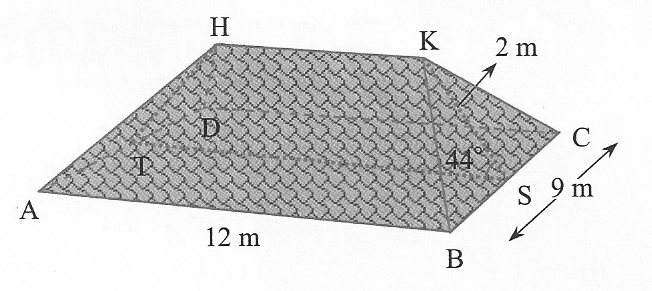
\includegraphics[scale=0.9]{roof}
              \end{center}
              \begin{enumerate}
                  \item The distance from line $HK$ to plane $ABCD$. \sol{}

                        Let the foot point of $K$ on plane $ABCD$ be $P$.
                        \begin{flalign*}
                            \text{In } \Delta KPS, \sin{\angle{KSP}} & = \frac{KP}{KS}   \\
                            \sin{44^\circ}                           & = \frac{KP}{2}    \\
                            KP                                       & = 2\sin{44^\circ} \\
                                                                     & \approx 1.39m
                        \end{flalign*}

                  \item The length of $HK$. \sol{}
                        \begin{flalign*}
                            \cos{\angle{KSP}} & = \frac{PS}{KS}   \\
                            \cos{44^\circ}    & = \frac{PS}{2}    \\
                            PS                & = 2\cos{44^\circ} \\
                                              & \approx 1.44m     \\
                            HK                & \approx 12 - 2PS  \\
                                              & \approx 12 - 2.88 \\
                                              & \approx 9.12m
                        \end{flalign*}

                  \item The angle formed by line $HA$ and plane $ABCD$. \sol{}

                        Let the foot point of $H$ on plane $ABCD$ be $Q$.
                        \begin{flalign*}
                            HA & = \sqrt{HT^2 + AT^2} \\
                               & = \sqrt{2^2 + 4.5^2} \\
                               & = \sqrt{24.25}cm     \\
                        \end{flalign*}
                        The angle formed by line $HA$ and plane $ABCD$ is $\angle{HAQ}$.
                        \begin{center}
                            \begin{tikzpicture}[scale=1.2]%,cap=round,>=latex]

                                \coordinate [label=left:$A$] (A) at (-1.5cm,-1.cm);
                                \coordinate [label=right:$Q$] (C) at (1.5cm,-1.0cm);
                                \coordinate [label=above:$H$] (B) at (1.5cm,1.0cm);
                                \draw (A) -- node[midway,above left] {$\sqrt{24.25}cm$} (B) -- node[midway, right] {$2\sin{44^\circ}cm$} (C) -- node[below] {} (A);

                                \draw (1.25cm,-1.0cm) rectangle (1.5cm,-0.75cm);
                                \tkzMarkAngle[size=0.5cm,color=black,mark=](C,A,B)
                            \end{tikzpicture}
                        \end{center}
                        \begin{flalign*}
                            \sin{\angle{HAQ}} & = \frac{HQ}{HA}                        \\
                            \sin{\angle{HAQ}} & = \frac{2\sin{44^\circ}}{\sqrt{24.25}} \\
                            \angle{HAQ}       & \approx 16.38^\circ
                        \end{flalign*}
              \end{enumerate}

        \item The length, width and height of a hall are $20m$, $15m$, and $4m$ respectively.
              Find:
              \begin{center}
                  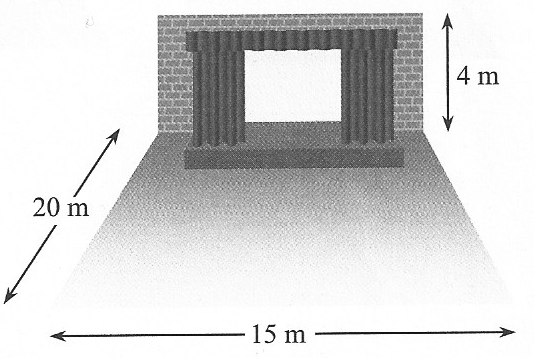
\includegraphics[scale=0.9]{hall}
              \end{center}
              \begin{enumerate}
                  \item The length of the diagonal of the hall. \sol{}
                        \begin{flalign*}
                            \text{Diagonal of floor} & = \sqrt{20^2 + 15^2} \\
                                                     & = \sqrt{625}m        \\
                                                     & = 25m                \\
                            \text{Diagonal of hall}  & = \sqrt{4^2 + 25^2}  \\
                                                     & = \sqrt{641}m        \\
                                                     & = 25.32m
                        \end{flalign*}

                  \item The angle formed by the diagonal and the floor of the hall. \sol{}
                        \begin{center}
                            \begin{tikzpicture}[scale=1.2]%,cap=round,>=latex]

                                \coordinate [label=left:$A$] (A) at (-1.5cm,-1.cm);
                                \coordinate [label=right:$C$] (C) at (1.5cm,-1.0cm);
                                \coordinate [label=above:$B$] (B) at (1.5cm,1.0cm);
                                \draw (A) -- node[midway,above left] {Diagonal of hall} (B) -- node[midway, right] {Wall height} (C) -- node[below] {Diagonal of floor} (A);

                                \draw (1.25cm,-1.0cm) rectangle (1.5cm,-0.75cm);
                                \tkzMarkAngle[size=0.5cm,color=black,mark=](C,A,B)
                            \end{tikzpicture}
                        \end{center}
                        \begin{center}
                            \begin{tikzpicture}[scale=1.2]%,cap=round,>=latex]

                                \coordinate [label=left:$A$] (A) at (-1.5cm,-1.cm);
                                \coordinate [label=right:$C$] (C) at (1.5cm,-1.0cm);
                                \coordinate [label=above:$B$] (B) at (1.5cm,1.0cm);
                                \draw (A) -- node[midway,above left] {$\sqrt{641}m$} (B) -- node[midway, right] {$4m$} (C) -- node[below] {$25m$} (A);

                                \draw (1.25cm,-1.0cm) rectangle (1.5cm,-0.75cm);
                                \tkzMarkAngle[size=0.5cm,color=black,mark=](C,A,B)
                            \end{tikzpicture}
                        \end{center}
                        \begin{flalign*}
                            \tan{\angle{BAC}} & = \frac{4}{25}     \\
                            \angle{BAC}       & \approx 9.09^\circ
                        \end{flalign*}
              \end{enumerate}

        \item In the diagram below, $ABCD$ represents a rectangular plank with length and
              width of $60cm$ and $36cm$ respectively, its base $BC$ is on the ground and the
              top of it lies on the wall. Assume that the distance between $BC$ and the
              corner of the wall is $12cm$, find the angle formed by the diagonal $BD$ of the
              plank and the ground.
              \begin{center}
                  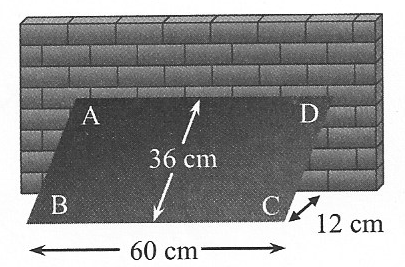
\includegraphics[scale=0.9]{wall}
              \end{center}
              \sol{}

              Let the footpoint of $D$ on the ground be $E$.
              \begin{flalign*}
                  BD & = \sqrt{BC^2 + CD^2} \\
                     & = \sqrt{60^2 + 36^2} \\
                     & = \sqrt{4896}cm      \\
                  DE & = \sqrt{DC^2 - CE^2} \\
                     & = \sqrt{36^2 - 12^2} \\
                     & = \sqrt{1152}cm      \\
              \end{flalign*}
              The angle formed by the diagonal $BD$ and the ground is $\angle{DBE}$.
              \begin{center}
                  \begin{tikzpicture}[scale=1.2]%,cap=round,>=latex]

                      \coordinate [label=left:$B$] (A) at (-1.5cm,-1.cm);
                      \coordinate [label=right:$E$] (C) at (1.5cm,-1.0cm);
                      \coordinate [label=above:$D$] (B) at (1.5cm,1.0cm);
                      \draw (A) -- node[midway,above left] {$\sqrt{4896}cm$} (B) -- node[midway, right] {$\sqrt{1152}cm$} (C) -- node[below] {} (A);

                      \draw (1.25cm,-1.0cm) rectangle (1.5cm,-0.75cm);
                      \tkzMarkAngle[size=0.5cm,color=black,mark=](C,A,B)
                  \end{tikzpicture}
              \end{center}
              \begin{flalign*}
                  \sin{\angle{DBE}} & = \frac{\sqrt{1152}}{\sqrt{4896}} \\
                  \angle{DBE}       & \approx 29.02^\circ
              \end{flalign*}
    \end{enumerate}

    \section{Angle Formed by Two Planes}

    There are three types positional relationship between two planes:

    \begin{enumerate}
        \item Two planes coincide with each other.
              \begin{center}
                  \begin{tikzpicture}
                      \draw (0,0)--(3,0);
                      \draw (3,0)--(4,1);
                      \draw (4,1)--(1,1)--(0,0);
                      \draw (0.2, 0.2) -- (3.2, 0.2);
                      \fill [color=gray,opacity=0.4] (0.2, 0.2) -- (3.2, 0.2) -- (4, 1) -- (1, 1) -- cycle;
                  \end{tikzpicture}
              \end{center}
        \item Two planes intersect with each other at a line.
              \begin{center}
                  \begin{tikzpicture}
                      \draw (0,0)--(3,0);
                      \draw (3,0)--(4,1);
                      \draw (4,1)--(1,1)--(0,0);
                      \filldraw [fill=gray!40] (0.9, 0) -- (2,1) -- (1, 1.5) -- (0, 0.5) -- (2, -0.6) -- (2.6, 0);
                  \end{tikzpicture}
              \end{center}
        \item Two planes are parallel to each other and do not intersect with each other.
              \begin{center}
                  \begin{tikzpicture}
                      \draw (0,0)--(3,0)--(4,1)--(1,1)--(0,0);
                      \filldraw [fill=gray!40] (-0.5,0.5)--(2.5,0.5)--(3.5,1.5)--(0.5,1.5)--(-0.5,0.5);
                  \end{tikzpicture}
              \end{center}
    \end{enumerate}

    Two non-parallel planes intersect with each other at a line, the line is called
    the \emph{common edge}. At any point on the common edge, draw a line
    perpendicular to the common edge on each plane, the acute angles formed by
    these two perpendicular lines are called \emph{the angle formed by the two
        planes}.
    \begin{center}
        \begin{tikzpicture}
            \draw (0,0)--(3,0)--(5,1.5)--(2,1.5)--(0,0);
            \draw (1.5, 0) -- (3.5, 1.5);
            \filldraw[fill=gray!40] (0, 0) -- (0.5, 1) -- (3.5, 1) -- (3, 0);
            \draw (1.5, 0) -- (2, 1);
            \draw [dashed] (1.5, 0) -- (2.85, 1);
            \draw [dashed] (0, 0) -- (1.35, 1);
            \draw (1.28, 0) -- (1.35, 0.15) -- (1.58, 0.15);
            \draw (1.7, 0.15) -- (1.9, 0.15) -- (1.7, 0);
            \node (O) at (1.5, 0) {};
            \node (x) at (2, 1) {};
            \node (z) at (2.9, 1) {};
            \pic [draw,
                angle radius=5mm, angle eccentricity=0.1] {angle = z--O--x};
        \end{tikzpicture}
    \end{center}

    \subsection{Practice 2}

    \begin{enumerate}
        \item The diagram below shows a cuboid with length of $12cm$, width of $10cm$ and
              height of $6cm$.
              \begin{center}
                  \begin{tikzpicture}[scale=1.4]
                      \draw (2,1,0) node [above] {$G$} --(0,1,0) node [above] {$H$} --(0,1,2) node [left] {$E$} --(2,1,2)node [above] {$F$} --(2,1,0) --(2,0,0) node [right] {$C$} node [midway, right] {$6cm$} --(2,0,2) node [below] {$B$}  node [midway, below right] {$10cm$} --(0,0,2) node [below] {$A$}  node [midway, below] {$12cm$} --(0,1,2);
                      \draw (2,1,2)--(2,0,2);
                      \draw[dashed](2,0,0)--(0,0,0) node [below] {$D$}--(0,1,0);
                      \draw[dashed](0,0,0)--(0,0,2);
                      \fill [color=gray, opacity=0.4] (0, 1, 0) -- (0, 1, 2) -- (2, 0, 2) -- (2, 0, 0) -- cycle;
                      \draw (1,1,0) circle (1pt) node [above] {$M$};
                  \end{tikzpicture}
              \end{center}
              \begin{enumerate}
                  \item Find the angle formed by plane $EBCH$ and plane $ABCD$. \sol{}

                        $\because$ $BC$ is the common edge of plane $EBCH$ and plane $ABCD$, $AB \perp BC$ and $EB \perp BC$.

                        $\therefore$ The angle formed by plane $EBCH$ and plane $ABCD$ is $\angle EBA$.
                        \begin{center}
                            \begin{tikzpicture}[scale=1.2]%,cap=round,>=latex]

                                \coordinate [label=left:$B$] (A) at (-1.5cm,-1.cm);
                                \coordinate [label=right:$A$] (C) at (1.5cm,-1.0cm);
                                \coordinate [label=above:$E$] (B) at (1.5cm,1.0cm);
                                \draw (A) -- node[midway,above left] {} (B) -- node[midway, right] {$6cm$} (C) -- node[below] {$12cm$} (A);

                                \draw (1.25cm,-1.0cm) rectangle (1.5cm,-0.75cm);
                                \tkzMarkAngle[size=0.5cm,color=black,mark=](C,A,B)
                            \end{tikzpicture}
                        \end{center}
                        \begin{flalign*}
                            \tan{\angle EAB} & = \frac{6}{12}      \\
                                             & = \frac{1}{2}       \\
                            \angle EAB       & \approx 26.57^\circ
                        \end{flalign*}

                  \item Assume that $M$ is a point on $HG$, find the angle formed by plane $MAB$ and
                        plane $ABCD$. \sol{}

                        $\because$ $AB$ is the common edge of plane $MAB$ and plane $ABCD$, $M$ is on $HG$, $HG \perp AB$, $BC \perp AB$.

                        $\therefore$ The angle formed by plane $MAB$ and plane $ABCD$ is $\angle GBC$.

                        \begin{center}
                            \begin{tikzpicture}[scale=1.2]%,cap=round,>=latex]

                                \coordinate [label=left:$B$] (A) at (-1.5cm,-1.cm);
                                \coordinate [label=right:$C$] (C) at (1.5cm,-1.0cm);
                                \coordinate [label=above:$G$] (B) at (1.5cm,1.0cm);
                                \draw (A) -- node[midway,above left] {} (B) -- node[midway, right] {$6cm$} (C) -- node[below] {$10cm$} (A);

                                \draw (1.25cm,-1.0cm) rectangle (1.5cm,-0.75cm);
                                \tkzMarkAngle[size=0.5cm,color=black,mark=](C,A,B)
                            \end{tikzpicture}
                        \end{center}
                        \begin{flalign*}
                            \tan{\angle GBC} & = \frac{6}{10}      \\
                                             & = \frac{3}{5}       \\
                            \angle GBC       & \approx 30.96^\circ
                        \end{flalign*}

              \end{enumerate}

        \item The diagram below shows a regular prism, its bases $ABC$ and $DEF$ are
              equilateral triangles with side length of $5cm$. Given that the height of the
              prism is $10cm$, find:
              \begin{center}
                  \begin{tikzpicture}[scale=1.4]
                      \draw (1,1.5,2) node [above] {$C$} --(2.5,1.5,0) --(3.5,0,0) node [right] {$E$} --(2,0,2) node [below right] {$B$}  node [midway, below right] {$10cm$} --(0,0,2) node [left] {$A$}  node [midway, below] {$5cm$} --(1,1.5,2);
                      \draw (1,1.5,2)--(2,0,2);
                      \draw[dashed](3.5,0,0)--(1.5,0,0) node [below] {$D$}--(2.5,1.5,0) node [above] {$F$};
                      \draw[dashed](1.5,0,0)--(0,0,2);
                      \fill[color=gray, opacity=0.4] (2.5, 1.5, 0) -- (0, 0, 2) -- (2, 0, 2);
                      \draw [dash pattern=on 1pt off 1pt] (2, 0, 2) -- (2.5, 1.5, 0);
                  \end{tikzpicture}
              \end{center}
              \begin{enumerate}
                  \item The length of $BF$. \sol{}
                        \begin{flalign*}
                            BF & = \sqrt{EF^2 + BE^2} \\
                               & = \sqrt{10^2 + 5^2}  \\
                               & = \sqrt{125}         \\
                               & \approx 11.18cm
                        \end{flalign*}

                  \item The angle formed by plane $ABF$ and plane $ABC$. \sol{}

                        Let the midpoint of $AB$ be $M$.
                        \begin{flalign*}
                            MF & = \sqrt{FB^2 - BM^2} \\
                               & = \sqrt{125 - 2.5^2} \\
                               & = \sqrt{118.75}cm
                        \end{flalign*}

                        $\because$ $AB$ is the common edge of plane $ABF$ and plane $ABC$, $MF \perp AB$, $CF \perp AB$.

                        $\therefore$ The angle formed by plane $ABF$ and plane $ABC$ is $\angle FMC$.
                        \begin{center}
                            \begin{tikzpicture}[scale=1.2]%,cap=round,>=latex]

                                \coordinate [label=left:$M$] (A) at (-1.5cm,-1.cm);
                                \coordinate [label=right:$C$] (C) at (1.5cm,-1.0cm);
                                \coordinate [label=above:$F$] (B) at (1.5cm,1.0cm);
                                \draw (A) -- node[midway,above left] {$\sqrt{118.75}cm$} (B) -- node[midway, right] {$10cm$} (C) -- node[below] {} (A);

                                \draw (1.25cm,-1.0cm) rectangle (1.5cm,-0.75cm);
                                \tkzMarkAngle[size=0.5cm,color=black,mark=](C,A,B)
                            \end{tikzpicture}
                        \end{center}
                        \begin{flalign*}
                            \sin\angle{FMC} & = \frac{FC}{MF}            \\
                                            & = \frac{10}{\sqrt{118.75}} \\
                            \angle{FMC}     & \approx 66.59^\circ
                        \end{flalign*}
              \end{enumerate}
    \end{enumerate}

    \subsection{Exercise 17.3}

    \begin{enumerate}
        \item The diagram below shows a cuboid with length of $8cm$, width of $6cm$ and
              height of $4cm$. Find the angle formed by plane $ABMN$ and $KLMN$.
              \begin{center}
                  \begin{tikzpicture}[scale=1.4]
                      \draw (2,1,0) node [above] {$D$} --(0,1,0) node [above] {$A$} --(0,1,2) node [left] {$B$} --(2,1,2)node [above] {$C$} --(2,1,0) --(2,0,0) node [right] {$N$} node [midway, right] {$4cm$} --(2,0,2) node [below] {$M$}  node [midway, below right] {$6cm$} --(0,0,2) node [below] {$L$} node [midway, below] {$8cm$} --(0,1,2);
                      \draw (2,1,2)--(2,0,2);
                      \draw[dashed](2,0,0)--(0,0,0) node [below] {$K$}--(0,1,0);
                      \draw[dashed](0,0,0)--(0,0,2);
                      \fill [color=gray, opacity=0.4] (0, 1, 0) -- (0, 1, 2) -- (2, 0, 2) -- (2, 0, 0) -- cycle;
                  \end{tikzpicture}
              \end{center}
              \sol{}

              $\because$ $MN$ is the common edge of $ABMN$ and $KLMN$, $LM \perp MN$ and $BM \perp MN$.

              $\therefore$ The angle formed by plane $ABMN$ and $KLMN$ is $\angle BML$.

              \begin{center}
                  \begin{tikzpicture}[scale=1.2]%,cap=round,>=latex]

                      \coordinate [label=left:$M$] (A) at (-1.5cm,-1.cm);
                      \coordinate [label=right:$L$] (C) at (1.5cm,-1.0cm);
                      \coordinate [label=above:$B$] (B) at (1.5cm,1.0cm);
                      \draw (A) -- node[midway,above left] {} (B) -- node[midway, right] {$4cm$} (C) -- node[below] {$8cm$} (A);

                      \draw (1.25cm,-1.0cm) rectangle (1.5cm,-0.75cm);
                      \tkzMarkAngle[size=0.5cm,color=black,mark=](C,A,B)
                  \end{tikzpicture}
              \end{center}
              \begin{flalign*}
                  \tan{\angle{BML}} & = \frac{BL}{LM}     \\
                                    & = \frac{4}{8}       \\
                                    & = \frac{1}{2}       \\
                  \angle{BML}       & \approx 26.57^\circ
              \end{flalign*}

        \item In the right prism shown below, $ABCD$ is a rectangle with length of $20cm$ and
              width of $12cm$, $BCRQ$ is a trapezoid, $\angle QBC$ and $\angle RCB$ are both
              right angles, $BQ = 5cm$, $CR = 10cm$. Find the angle formed by plane $PQRS$
              and plane $ABCD$.
              \begin{center}
                  \begin{tikzpicture}[scale=1.4]
                      \draw (2,1,0) node [above] {$R$} --(0,1,0) node [above] {$S$} --(0,0.5,2) node [left] {$P$} --(2,0.5,2)node [above=6pt,left=-2pt] {$Q$} --(2,1,0) --(2,0,0) node [right] {$C$} node [midway, right] {$10cm$} --(2,0,2) node [below] {$B$}  node [midway, below right] {$12cm$} --(0,0,2) node [below] {$A$} node [midway, below] {$20cm$} --(0,0.5,2);
                      \draw (2,0.5,2)--(2,0,2) node [midway, left] {$5cm$};
                      \draw[dashed](2,0,0)--(0,0,0) node [above = 2pt, left] {$D$}--(0,1,0);
                      \draw[dashed](0,0,0)--(0,0,2);
                      \draw (2, 0.2, 0) -- (2, 0.2, 0.3) -- (2, 0.0, 0.3);
                      \draw (2, 0.2, 2) -- (2, 0.2, 1.7) -- (2, 0.0, 1.7);
                  \end{tikzpicture}
              \end{center}
              \sol{}

              Let the midpoint of $RC$ and $SD$ be $E$ and $F$ respectively.

              $\because$ $PQEF \newparallel ABCD$, $PQ$ is the common edge of $PQRS$ and $PQER$, $PQ \perp QE$, and $PQ \perp QR$.

              $\therefore$ The angle formed by plane $PQRS$ and $ABCD$ is $\angle RQE$.
              \begin{center}
                  \begin{tikzpicture}[scale=1.2]%,cap=round,>=latex]

                      \coordinate [label=left:$Q$] (A) at (-1.5cm,-1.cm);
                      \coordinate [label=right:$E$] (C) at (1.5cm,-1.0cm);
                      \coordinate [label=above:$R$] (B) at (1.5cm,1.0cm);
                      \draw (A) -- node[midway,above left] {} (B) -- node[midway, right] {$5cm$} (C) -- node[below] {$12cm$} (A);

                      \draw (1.25cm,-1.0cm) rectangle (1.5cm,-0.75cm);
                      \tkzMarkAngle[size=0.5cm,color=black,mark=](C,A,B)
                  \end{tikzpicture}
              \end{center}
              \begin{flalign*}
                  \tan{\angle RQE} & = \frac{RE}{QE}     \\
                                   & = \frac{5}{12}      \\
                  \angle RQE       & \approx 22.62^\circ
              \end{flalign*}

        \item The diagram below shows a cuboid, $AB = 8cm$, $BC = 6cm$, $CT = 5cm$, $X$ is
              the midpoint of $TU$. Find:
              \begin{center}
                  \begin{tikzpicture}[scale=1.4]
                      \draw (2,1,0) node [above] {$T$} --(0,1,0) node [above] {$U$} --(0,1,2) node [left] {$R$} --(2,1,2)node [above] {$S$} --(2,1,0) --(2,0,0) node [right] {$C$} node [midway, right] {$5cm$} --(2,0,2) node [below] {$B$}  node [midway, below right] {$6cm$} --(0,0,2) node [below] {$A$}  node [midway, below] {$8cm$} --(0,1,2);
                      \draw (2,1,2)--(2,0,2);
                      \draw[dashed](2,0,0)--(0,0,0) node [below] {$D$}--(0,1,0);
                      \draw[dashed](0,0,0)--(0,0,2);
                      \fill [color=gray, opacity=0.4] (2, 0, 2) -- (0, 0, 2) -- (1,1,0) -- cycle;
                      \draw (1,1,0) circle (1pt) node [above] {$X$};
                  \end{tikzpicture}
              \end{center}
              \begin{enumerate}
                  \item The angle formed by plane $XAB$ and plane $ABCD$. \sol{}

                        Let the midpoint of $AB$ and $CD$ be $E$ and $F$ respectively.

                        $\because$ $AB$ is the common edge of $ABCD$ and $XAB$, $AB \perp XE$, and $AB \perp EF$.

                        $\therefore$ The angle formed by plane $ABCD$ and $XAB$ is $\angle XEF$.
                        \begin{center}
                            \begin{tikzpicture}[scale=1.2]%,cap=round,>=latex]

                                \coordinate [label=left:$E$] (A) at (-1.5cm,-1.cm);
                                \coordinate [label=right:$F$] (C) at (1.5cm,-1.0cm);
                                \coordinate [label=above:$X$] (B) at (1.5cm,1.0cm);
                                \draw (A) -- node[midway,above left] {} (B) -- node[midway, right] {$5cm$} (C) -- node[below] {$6cm$} (A);

                                \draw (1.25cm,-1.0cm) rectangle (1.5cm,-0.75cm);
                                \tkzMarkAngle[size=0.5cm,color=black,mark=](C,A,B)
                            \end{tikzpicture}
                        \end{center}
                        \begin{flalign*}
                            \tan{\angle XEF} & = \frac{XF}{EF}     \\
                                             & = \frac{5}{6}       \\
                            \angle XEF       & \approx 39.81^\circ
                        \end{flalign*}

                  \item The angle formed by plane $BCUR$ and plane $ADUR$. \sol{}

                        $\because$ $UR$ is the common edge of $BCUR$ and $ADUR$, $UR \perp RB$, and $UR \perp AR$.

                        $\therefore$ The angle formed by plane $BCUR$ and $ADUR$ is $\angle BRA$.
                        \begin{center}
                            \begin{tikzpicture}[scale=1.2]%,cap=round,>=latex]

                                \coordinate [label=left:$R$] (A) at (-1.5cm,-1.cm);
                                \coordinate [label=right:$A$] (C) at (1.5cm,-1.0cm);
                                \coordinate [label=above:$B$] (B) at (1.5cm,1.0cm);
                                \draw (A) -- node[midway,above left] {} (B) -- node[midway, right] {$8cm$} (C) -- node[below] {$5cm$} (A);

                                \draw (1.25cm,-1.0cm) rectangle (1.5cm,-0.75cm);
                                \tkzMarkAngle[size=0.5cm,color=black,mark=](C,A,B)
                            \end{tikzpicture}
                        \end{center}
                        \begin{flalign*}
                            \tan{\angle BRA} & = \frac{BA}{RA}     \\
                                             & = \frac{8}{5}       \\
                            \angle BRA       & \approx 57.99^\circ
                        \end{flalign*}

                  \item The angle formed by plane $ABTU$ and plane $ABCD$. \sol{}

                        $\because$ $AB$ is the common edge of $ABTU$ and $ABCD$, $AB \perp TB$, and $AB \perp BC$.

                        $\therefore$ The angle formed by plane $ABTU$ and $ABCD$ is $\angle TBC$.
                        \begin{center}
                            \begin{tikzpicture}[scale=1.2]%,cap=round,>=latex]

                                \coordinate [label=left:$B$] (A) at (-1.5cm,-1.cm);
                                \coordinate [label=right:$C$] (C) at (1.5cm,-1.0cm);
                                \coordinate [label=above:$T$] (B) at (1.5cm,1.0cm);
                                \draw (A) -- node[midway,above left] {} (B) -- node[midway, right] {$5cm$} (C) -- node[below] {$6cm$} (A);

                                \draw (1.25cm,-1.0cm) rectangle (1.5cm,-0.75cm);
                                \tkzMarkAngle[size=0.5cm,color=black,mark=](C,A,B)
                            \end{tikzpicture}
                        \end{center}
                        \begin{flalign*}
                            \tan{\angle TBC} & = \frac{TC}{BC}     \\
                                             & = \frac{5}{6}       \\
                            \angle TBC       & \approx 39.81^\circ
                        \end{flalign*}
              \end{enumerate}

        \item The diagram below shows a right pyramid, its bases $ABE$ and $DCF$ are
              right-angled triangles. Given that $AE = 4cm$, $BE = \frac{2}{3}EF$, $EF =
                  4DF$, find the angle formed by plane $ABCD$ and plane $BCFE$.
              \begin{center}
                  \begin{tikzpicture}[scale=1.1]
                      \draw (3,1,0) node [above] {$D$} --(0,1,0) node [above] {$A$};
                      \draw (3, 1, 0)--(3,0,0) node [right] {$F$} --(3,0,2)node [below] {$C$}--(0,0,2) node [below] {$B$};
                      \draw (0,1,0) -- (0,0,2);
                      \draw (3,1,0) -- (3,0,2);
                      \draw (3, 0.2, 0) -- (3, 0.2, 0.3) -- (3, 0.0, 0.3);
                      \draw[dashed](3,0,0)--(0,0,0) node [below=6pt, right=-6pt] {$E$}--(0,1,0)  node [midway,right] {$4cm$};
                      \draw[dashed](0,0,0)--(0,0,2);
                      \draw[dash pattern=on 1pt off 1pt] (0, 1, 0) -- (3,0,2);
                  \end{tikzpicture}
              \end{center}
              \sol{}
              \begin{flalign*}
                  EF & = 4DF            \\
                     & = 4 \times 4     \\
                     & = 16cm           \\
                  BE & = \frac{2}{3}EF  \\
                     & = \frac{32}{3}cm \\
              \end{flalign*}

              $\because$ $BC$ is the common edge of $ABCD$ and $BCFE$, $BC \perp CD$, and $BC \perp CF$.

              $\therefore$ The angle formed by plane $ABCD$ and $BCFE$ is $\angle DCF$.
              \begin{center}
                  \begin{tikzpicture}[scale=1.2]%,cap=round,>=latex]

                      \coordinate [label=left:$C$] (A) at (-1.5cm,-1.cm);
                      \coordinate [label=right:$F$] (C) at (1.5cm,-1.0cm);
                      \coordinate [label=above:$D$] (B) at (1.5cm,1.0cm);
                      \draw (A) -- node[midway,above left] {} (B) -- node[midway, right] {$4cm$} (C) -- node[below] {$\frac{32}{3}cm$} (A);

                      \draw (1.25cm,-1.0cm) rectangle (1.5cm,-0.75cm);
                      \tkzMarkAngle[size=0.5cm,color=black,mark=](C,A,B)
                  \end{tikzpicture}
              \end{center}
              \begin{flalign*}
                  \tan{\angle DCF} & = \frac{DF}{CF}          \\
                                   & = \frac{4}{\frac{32}{3}} \\
                  \angle DCF       & \approx 20.56^\circ
              \end{flalign*}

        \item In the pyramid shown below, $PQT$, $SPT$, and $SRT$ are all right-angled
              triangles, $PQRS$ is a triangle. Given that $PQ = 5cm$, $RT = 13cm$, $PT =
                  20cm$. Find:
              \begin{center}
                  \tdplotsetmaincoords{70}{-20}
                  \begin{tikzpicture}[scale=0.7,tdplot_main_coords,line cap=butt,line join=bevel]
                      \draw (-2, 2, 0) node [left] {$P$} -- (-1,-0.5,0) node [below] {$Q$} node [midway, left=8pt,below=-2pt] {$5cm$} -- (3,-0.5,0) node [right] {$R$};
                      \draw [dashed] (3, -0.5, 0) -- (2,2,0) node [below=8pt, left=-6pt] {$S$} -- (-2,2,0);
                      \draw [dashed] (2,2,0) -- (2,2,5) node [above] {$T$};
                      \draw (-1,-0.5,0) -- (2,2,5) -- (3,-0.5,0) node [midway, right] {$13cm$};
                      \draw (2,2,5) -- (-2,2,0) node [midway, above left] {$20cm$};
                      \draw (1.71, 2, 0) -- (2, 2.8, 0) -- (2, 2, 0.32) -- (2, 1.2, 0.5) -- (2, 1.2, 0.15);
                      \draw (-1.95, 1.6, 0.4) -- (-1.9, 0.9, 0.5) -- (-2.05, 1, 0.25);
                  \end{tikzpicture}
              \end{center}
              \begin{enumerate}
                  \item The height of the prism. \sol{}
                        \begin{flalign*}
                            \text{Height of the prism} & = TS                 \\
                                                       & = \sqrt{TR^2 - RS^2} \\
                                                       & = \sqrt{13^2 - 5^2}  \\
                                                       & = 12cm
                        \end{flalign*}
                  \item The angle formed by line $TQ$ and plane $PST$. \sol{}

                        The angle formed by line $TQ$ and plane $PST$ is $\angle QTP$.
                        \begin{center}
                            \begin{tikzpicture}[scale=1.2]%,cap=round,>=latex]

                                \coordinate [label=left:$T$] (A) at (-1.5cm,-1.cm);
                                \coordinate [label=right:$P$] (C) at (1.5cm,-1.0cm);
                                \coordinate [label=above:$Q$] (B) at (1.5cm,1.0cm);
                                \draw (A) -- node[midway,above left] {} (B) -- node[midway, right] {$20cm$} (C) -- node[below] {$5cm$} (A);

                                \draw (1.25cm,-1.0cm) rectangle (1.5cm,-0.75cm);
                                \tkzMarkAngle[size=0.5cm,color=black,mark=](C,A,B)
                            \end{tikzpicture}
                        \end{center}
                        \begin{flalign*}
                            \tan{\angle QTP} & = \frac{PQ}{PT}     \\
                                             & = \frac{5}{20}      \\
                                             & = \frac{1}{4}       \\
                            \angle QTP       & \approx 14.04^\circ
                        \end{flalign*}

                  \item The angle formed by plane $RST$ and $PQT$. \sol{}

                        The angle formed by plane $RST$ and $PQT$ is $\angle STP$.
                        \begin{flalign*}
                            \text{In } \Delta{TRS},\ TS & = \sqrt{TR^2 - SR^2} \\
                                                        & = \sqrt{13^2 - 5^2}  \\
                                                        & = 12cm               \\
                        \end{flalign*}
                        \begin{center}
                            \begin{tikzpicture}[scale=1.2]%,cap=round,>=latex]

                                \coordinate [label=left:$T$] (A) at (-1.5cm,-1.cm);
                                \coordinate [label=right:$P$] (C) at (1.5cm,-1.0cm);
                                \coordinate [label=above:$S$] (B) at (1.5cm,1.0cm);
                                \draw (A) -- node[midway,above left] {$20cm$} (B) -- node[midway, right] {$12cm$} (C) -- node[below] {} (A);

                                \draw (1.25cm,-1.0cm) rectangle (1.5cm,-0.75cm);
                                \tkzMarkAngle[size=0.5cm,color=black,mark=](C,A,B)
                            \end{tikzpicture}
                            \begin{flalign*}
                                \sin{\angle{STP}} & = \frac{SP}{TS}     \\
                                                  & = \frac{12}{20}     \\
                                                  & = \frac{3}{5}       \\
                                \angle{STP}       & \approx 53.13^\circ
                            \end{flalign*}
                        \end{center}
              \end{enumerate}

        \item The diagram below shows a right prism, its base $BCGF$ is a trapezoid, $BC = BF
                  = 12cm$, $FG = 16cm$. The lateral face $EFGH$ is a square, and is
              perependicular to another lateral face $ABFE$. Find:
              \begin{center}
                  \begin{tikzpicture}[scale=1.4]
                      \draw (1.5,1.5,0) node [above] {$D$} --(0,1.5,0) node [above] {$A$} --(0,1.5,2) node [left] {$B$} --(1.5,1.5,2)node [above] {$C$} --(1.5,1.5,0) --(2,0,0) node [right] {$H$} --(2,0,2) node [below] {$G$} --(0,0,2) node [below] {$F$} node [midway, below] {$16cm$} --(0,1.5,2) node [midway, left=4pt] {$12cm$};
                      \draw (1.5,1.5,2)--(2,0,2);
                      \draw[dashed](2,0,0)--(0,0,0) node [below] {$E$}--(0,1.5,0);
                      \draw[dashed](0,0,0)--(0,0,2);
                      \fill [color=gray, opacity=0.4] (0, 1.5, 0) -- (0, 1.5, 2) -- (2, 0, 0) -- cycle;
                      \node (a) at (0,1.5,2) {};
                      \node (b) at (1.5,1.5,2) {};
                      \node (c) at (0,0,2) {};
                      \tkzMarkSegment[pos=.45,mark=||](a,b);
                      \tkzMarkSegment[pos=.5,mark=||](a,c);
                      \draw (0, 0.15, 0) -- (0.15, 0.15, 0) -- (0.15, 0, 0);
                      \draw (0, 0.15, 2) -- (0.15, 0.15, 2) -- (0.15, 0, 2);
                  \end{tikzpicture}
              \end{center}
              \begin{enumerate}
                  \item The angle formed by plane $CDHG$ and plane $EFGH$. \sol{}

                        Let the foot point of $C$ be $K$. \\

                        $\because$ $GH$ is the common edge of the plane $CDHG$ and plane $EFGH$, $CG \perp GH$, and $KG \perp GH$.

                        $\therefore$ The angle formed by plane $CDHG$ and plane $EFGH$ is $\angle CGK$.
                        \begin{flalign*}
                            KG & = FG - FK \\
                               & = 16 - 12 \\
                               & = 4cm
                        \end{flalign*}
                        \begin{center}
                            \begin{tikzpicture}[scale=1.2]%,cap=round,>=latex]
                                \coordinate [label=left:$G$] (A) at (-1.5cm,-1.cm);
                                \coordinate [label=right:$K$] (C) at (1.5cm,-1.0cm);
                                \coordinate [label=above:$C$] (B) at (1.5cm,1.0cm);
                                \draw (A) -- node[midway,above left] {} (B) -- node[midway, right] {$12cm$} (C) -- node[below] {$4cm$} (A);

                                \draw (1.25cm,-1.0cm) rectangle (1.5cm,-0.75cm);
                                \tkzMarkAngle[size=0.5cm,color=black,mark=](C,A,B)
                            \end{tikzpicture}
                        \end{center}
                        \begin{flalign*}
                            \tan{\angle{CGK}} & = \frac{CK}{KG}       \\
                                              & = \frac{12}{4}        \\
                                              & = 3                   \\
                            \angle{CGK}       & \approx 71.57^{\circ}
                        \end{flalign*}

                  \item The angle formed by plane $ABH$ and plane $ABFE$. \sol{}

                        $\because$ $AB$ is the common edge of the plane $ABH$ and plane $ABFE$, $AB \perp AH$ and $AB \perp AE$.

                        $\therefore$ The angle formed by plane $ABH$ and plane $ABFE$ is $\angle HAE$.
                        \begin{center}
                            \begin{tikzpicture}[scale=1.2]%,cap=round,>=latex]
                                \coordinate [label=left:$A$] (A) at (-1.5cm,-1.cm);
                                \coordinate [label=right:$E$] (C) at (1.5cm,-1.0cm);
                                \coordinate [label=above:$H$] (B) at (1.5cm,1.0cm);
                                \draw (A) -- node[midway,above left] {} (B) -- node[midway, right] {$16cm$} (C) -- node[below] {$12cm$} (A);

                                \draw (1.25cm,-1.0cm) rectangle (1.5cm,-0.75cm);
                                \tkzMarkAngle[size=0.5cm,color=black,mark=](C,A,B)
                            \end{tikzpicture}
                        \end{center}
                        \begin{flalign*}
                            \tan{\angle{HAE}} & = \frac{HE}{AE}       \\
                                              & = \frac{16}{12}       \\
                                              & = \frac{4}{3}         \\
                            \angle{HAE}       & \approx 53.13^{\circ}
                        \end{flalign*}
              \end{enumerate}

        \item In the cuboid shown below, $BC = 8cm$, $CD = 6cm$, $BQ = 10cm$. Given that $M$
              is the midpoint of $PQ$. Find:
              \begin{center}
                  \begin{tikzpicture}[scale=1.2]
                      \draw (2,3,0) node [above] {$S$} --(0,3,0) node [above] {$P$} --(0,3,2) node [left] {$Q$} --(2,3,2)node [above] {$R$} --(2,3,0) --(2,0,0) node [right] {$D$} --(2,0,2) node [below] {$C$}  node [midway, below right] {$6cm$} --(0,0,2) node [below] {$B$}  node [midway, below] {$8cm$} --(0,3,2) node [midway, left] {$10cm$};
                      \draw (2,3,2)--(2,0,2);
                      \draw[dashed](2,0,0)--(0,0,0) node [above=2pt, left] {$A$}--(0,3,0);
                      \draw[dashed](0,0,0)--(0,0,2);
                      \fill [color=gray, opacity=0.4] (0, 3, 1) -- (0,0,0) -- (2, 0, 0) -- cycle;
                      \draw (0,3,1) circle (1pt) node [above] {$M$};
                  \end{tikzpicture}
              \end{center}
              \begin{enumerate}
                  \item The angle formed by line $MD$ and plane $PQBA$. \sol{}

                        The angle formed by line $MD$ and plane $PQBA$ is $\angle DMA$.
                        \begin{flalign*}
                            \text{In } \Delta MPA,\ MA & = \sqrt{PA^2 + MP^2} \\
                                                       & = \sqrt{10^2 + 3^2}  \\
                                                       & = \sqrt{109}cm
                        \end{flalign*}
                        \begin{center}
                            \begin{tikzpicture}[scale=1.2]%,cap=round,>=latex]
                                \coordinate [label=left:$M$] (A) at (-1.5cm,-1.cm);
                                \coordinate [label=right:$A$] (C) at (1.5cm,-1.0cm);
                                \coordinate [label=above:$D$] (B) at (1.5cm,1.0cm);
                                \draw (A) -- node[midway,above left] {} (B) -- node[midway, right] {$8cm$} (C) -- node[below] {$\sqrt{109}cm$} (A);

                                \draw (1.25cm,-1.0cm) rectangle (1.5cm,-0.75cm);
                                \tkzMarkAngle[size=0.5cm,color=black,mark=](C,A,B)
                            \end{tikzpicture}
                        \end{center}
                        \begin{flalign*}
                            \tan{\angle{DMA}} & = \frac{DA}{MA}        \\
                                              & = \frac{8}{\sqrt{109}} \\
                            \angle{DMA}       & \approx 37.46^{\circ}
                        \end{flalign*}

                  \item The angle formed by plane $AMD$ and plane $ABCD$. \sol{}

                        Let the midpoint of $AB$ be $E$.\\

                        $\because$ $AD$ is the common edge of plane $AMD$ and plane $ABCD$, $AM \perp AD$, and $EA \perp AD$.

                        $\therefore$ The angle formed by plane $AMD$ and plane $ABCD$ is $\angle MAE$.
                        \begin{center}
                            \begin{tikzpicture}[scale=1.2]%,cap=round,>=latex]
                                \coordinate [label=left:$A$] (A) at (-1.5cm,-1.cm);
                                \coordinate [label=right:$E$] (C) at (1.5cm,-1.0cm);
                                \coordinate [label=above:$M$] (B) at (1.5cm,1.0cm);
                                \draw (A) -- node[midway,above left] {$\sqrt{109}cm$} (B) -- node[midway, right] {$10cm$} (C) -- node[below] {} (A);

                                \draw (1.25cm,-1.0cm) rectangle (1.5cm,-0.75cm);
                                \tkzMarkAngle[size=0.5cm,color=black,mark=](C,A,B)
                            \end{tikzpicture}
                        \end{center}
                        \begin{flalign*}
                            \sin{\angle{MAE}} & = \frac{ME}{MA}         \\
                                              & = \frac{10}{\sqrt{109}} \\
                            \angle{MAE}       & \approx 73.30^{\circ}
                        \end{flalign*}
              \end{enumerate}

        \item The diagram below shows a pyramid with an isoceles triangle base. Given that
              $CD = CE = 5cm$, $ED = 6cm$, $ACD$ is a right-angled triangle, $B$ is a point
              on $AC$, $AD = 2cm$, $BC = 4cm$. Find:
              \begin{center}
                  \tdplotsetmaincoords{70}{70}
                  \begin{tikzpicture}[scale=0.6,tdplot_main_coords,declare function={d=6;}]
                      \path (0,0,0)       coordinate (A) node [left] {$E$}
                      (d,0,0)        coordinate (C) node [below] {$D$}
                      (d/2,{d*sqrt(3)/2},0)    coordinate (B) node [right] {$C$}
                      (d/2,{d*sqrt(3)/2 - 0.15} ,d-1.5) coordinate (F) node [right] {$B$}
                      (d/2,d/2 + 2,{d/sqrt(2) + 2}) coordinate (D) node [above] {$A$}
                      ($ (A)!0.5!(C) $) coordinate (M);
                      \foreach \p/\g in {A/-90,B/-90,C/-90,D/90}
                      \path (\p)+(\g:3mm);
                      \draw (F) circle (1.2pt);
                      \draw (D) -- (A) (D) -- (B) (D) -- (C) (A) -- (C) -- (B);
                      \draw [dashed] (A) -- (B);
                      \path (D) -- (F) node [midway, right] {$2cm$};
                      \path (B) -- (F) node [midway, right] {$4cm$};
                      \path (C) -- (B) node [midway, right=12pt, below=4pt] {$5cm$};
                      \path (A) -- (C) node [midway, left=14pt, below=-4pt] {$6cm$};
                      \fill [color=gray, opacity=0.4] (A) -- (C) -- (F) -- cycle;
                      \draw (d/2,{d*sqrt(3)/2},0.5) -- (d/2,{d*sqrt(3)/2 - 0.4} ,0.4) -- (d/2,{d*sqrt(3)/2 - 0.4} ,-0.1);
                      \tkzMarkSegment[pos=.45,mark=||](A,B);
                      \tkzMarkSegment[pos=.45,mark=||](B,C);
                  \end{tikzpicture}
              \end{center}
              \begin{enumerate}
                  \item The angle formed by plane $BDE$ and plane $CDE$. \sol{}

                        Let the midpoint of $ED$ be $M$.\\

                        $\because$ $DE$ is the common edge of plane $BDE$ and plane $CDE$, $BM \perp DE$, and $CM \perp DE$.

                        $\therefore$ The angle formed by plane $BDE$ and plane $CDE$ is $\angle BMC$.
                        \begin{flalign*}
                            MC & = \sqrt{DC^2 - DM^2} \\
                               & = \sqrt{5^2 - 3^2}   \\
                               & = 4cm
                        \end{flalign*}
                        \begin{center}
                            \begin{tikzpicture}[scale=1.2]%,cap=round,>=latex]
                                \coordinate [label=left:$M$] (A) at (-1.5cm,-1.cm);
                                \coordinate [label=right:$C$] (C) at (1.5cm,-1.0cm);
                                \coordinate [label=above:$B$] (B) at (1.5cm,1.0cm);
                                \draw (A) -- node[midway,above left] {} (B) -- node[midway, right] {$4cm$} (C) -- node[below] {$4cm$} (A);

                                \draw (1.25cm,-1.0cm) rectangle (1.5cm,-0.75cm);
                                \tkzMarkAngle[size=0.5cm,color=black,mark=](C,A,B)
                            \end{tikzpicture}
                        \end{center}
                        \begin{flalign*}
                            \tan{\angle{BMC}} & = \frac{BC}{CM} \\
                                              & = \frac{4}{4}   \\
                                              & = 1             \\
                            \angle{BMC}       & = 45^{\circ}
                        \end{flalign*}

                  \item The angle formed by the plane $ADE$ and $CDE$. \sol{}

                        $\because$ $DE$ is the common edge of plane $ADE$ and plane $CDE$, $CM \perp DE$, and $AM \perp DE$.

                        $\therefore$ The angle formed by plane $ADE$ and plane $CDE$ is $\angle AMC$.
                        \begin{center}
                            \begin{tikzpicture}[scale=1.2]%,cap=round,>=latex]
                                \coordinate [label=left:$M$] (A) at (-1.5cm,-1.cm);
                                \coordinate [label=right:$C$] (C) at (1.5cm,-1.0cm);
                                \coordinate [label=above:$A$] (B) at (1.5cm,1.0cm);
                                \draw (A) -- node[midway,above left] {} (B) -- node[midway, right] {$6cm$} (C) -- node[below] {$4cm$} (A);

                                \draw (1.25cm,-1.0cm) rectangle (1.5cm,-0.75cm);
                                \tkzMarkAngle[size=0.5cm,color=black,mark=](C,A,B)
                            \end{tikzpicture}
                        \end{center}
                        \begin{flalign*}
                            \tan{\angle{AMC}} & = \frac{AC}{CM}       \\
                                              & = \frac{6}{4}         \\
                                              & = \frac{3}{2}         \\
                            \angle{AMC}       & \approx 56.31^{\circ}
                        \end{flalign*}
              \end{enumerate}

        \item The diagram below shows a regular pyramid with a square base. Given that $PQ =
                  15cm$, $PV = 20cm$. Find:
              \begin{center}
                  \begin{tikzpicture}
                      \tikzstyle{point}=[circle,thick,draw=black,fill=black,inner sep=0pt,minimum width=4pt,minimum height=4pt]
                      \node (a) at (0,0) {};
                      \node (b) at (2.5,0) {};
                      \node (c) at (3.5,1) {};
                      \node (d) at (1,1) {};
                      \node (e) at (1.75,3) {};
                      \draw (a.center) node [below left] {$P$} -- (b.center) node [below] {$Q$} node [midway, below] {$15cm$} -- (c.center) node [ right] {$R$} -- (e.center) node [above] {$V$} -- (b.center);
                      \draw (a.center) -- (e.center) node [midway, left=4pt] {$20cm$};
                      \draw[dashed] (a.center) -- (d.center) -- (c.center);
                      \draw[dashed] (d.center) node [below] {$S$} -- (e.center);
                  \end{tikzpicture}
              \end{center}
              \begin{enumerate}
                  \item The angle formed by line $PV$ and plane $PQRS$. \sol{}

                        Let the footpoint of $V$ be $M$.

                        The angle formed by line $PV$ and plane $PQRS$ is $\angle{VPM}$.
                        \begin{flalign*}
                            PR & = \sqrt{PQ^2 + QR^2}   \\
                               & = \sqrt{15^2 + 15^2}   \\
                               & = 15\sqrt{2}cm         \\
                            PM & = \frac{PR}{2}         \\
                               & = \frac{15\sqrt{2}}{2}
                        \end{flalign*}
                        \begin{center}
                            \begin{tikzpicture}[scale=1.2]%,cap=round,>=latex]
                                \coordinate [label=left:$P$] (A) at (-1.5cm,-1.cm);
                                \coordinate [label=right:$M$] (C) at (1.5cm,-1.0cm);
                                \coordinate [label=above:$V$] (B) at (1.5cm,1.0cm);
                                \draw (A) -- node[midway,above left] {$20cm$} (B) -- node[midway, right] {} (C) -- node[below] {$\frac{15\sqrt{2}}{2}cm$} (A);

                                \draw (1.25cm,-1.0cm) rectangle (1.5cm,-0.75cm);
                                \tkzMarkAngle[size=0.5cm,color=black,mark=](C,A,B)
                            \end{tikzpicture}
                        \end{center}
                        \begin{flalign*}
                            \cos{\angle{VPM}} & = \frac{PM}{PV}                   \\
                                              & = \frac{\frac{15\sqrt{2}}{2}}{20} \\
                                              & = \frac{3\sqrt{2}}{8}             \\
                            \angle{VPM}       & \approx 57.97^{\circ}
                        \end{flalign*}

                  \item The angle formed by the lateral faces and the base of the pyramid. \sol{}
                        \begin{flalign*}
                            VM & = \sqrt{VP^2 - PM^2}                                  \\
                               & = \sqrt{20^2 - {\left(\frac{15\sqrt{2}}{2}\right)}^2} \\
                               & = \sqrt{287.5}cm
                        \end{flalign*}

                        Let the midpoint of $PQ$ be $N$.

                        The angle formed by the lateral faces and the base of the pyramid is
                        $\angle{VNM}$.
                        \begin{center}
                            \begin{tikzpicture}[scale=1.2]%,cap=round,>=latex]
                                \coordinate [label=left:$N$] (A) at (-1.5cm,-1.cm);
                                \coordinate [label=right:$M$] (C) at (1.5cm,-1.0cm);
                                \coordinate [label=above:$V$] (B) at (1.5cm,1.0cm);
                                \draw (A) -- node[midway,above left] {} (B) -- node[midway, right] {$\sqrt{287.5}cm$} (C) -- node[below] {$7.5cm$} (A);

                                \draw (1.25cm,-1.0cm) rectangle (1.5cm,-0.75cm);
                                \tkzMarkAngle[size=0.5cm,color=black,mark=](C,A,B)
                            \end{tikzpicture}
                        \end{center}
                        \begin{flalign*}
                            \tan{\angle{VNM}} & = \frac{VM}{NM}            \\
                                              & = \frac{\sqrt{287.5}}{7.5} \\
                            \angle{VNM}       & \approx 66.14^{\circ}
                        \end{flalign*}
              \end{enumerate}

        \item The diagram below shows a right pyramid with lateral edges of $13cm$. Its base
              $ABCD$ is a rectangle with length of $12cm$ and width of $10cm$. Find:
              \begin{center}
                  \begin{tikzpicture}
                      \tikzstyle{point}=[circle,thick,draw=black,fill=black,inner sep=0pt,minimum width=4pt,minimum height=4pt]
                      \node (a) at (0,0) {};
                      \node (b) at (2.5,0) {};
                      \node (c) at (3.5,1) {};
                      \node (d) at (1,1) {};
                      \node (e) at (1.75,3) {};
                      \draw (a.center) node [below left] {$A$} -- (b.center) node [below] {$B$} node [midway, below] {$12cm$} -- (c.center) node [ right] {$C$} node [midway, right=12pt, below=-4pt] {$10cm$} -- (e.center) node [above] {$V$} -- (b.center);
                      \draw (a.center) -- (e.center) node [midway, left=4pt] {$13cm$};
                      \draw[dashed] (a.center) -- (d.center) -- (c.center);
                      \draw[dashed] (d.center) node [below] {$D$} -- (e.center);
                  \end{tikzpicture}
              \end{center}
              \begin{enumerate}
                  \item The angle formed by plane $VBC$ and plane $ABCD$. \sol{}

                        Let the midpoint of $BC$ be $E$, and the footpoint of $V$ be $M$.

                        $\because$ $BC$ is the common edge of plane $VBC$ and plane $ABCD$, $VE \perp BC$, and $ME \perp BC$.

                        $\therefore$ The angle formed by plane $VBC$ and plane $ABCD$ is $\angle{VEM}$.
                        \begin{flalign*}
                            VE & = \sqrt{VB^2 - BE^2} \\
                               & = \sqrt{13^2 - 5^2}  \\
                               & = 12cm
                        \end{flalign*}
                        \begin{center}
                            \begin{tikzpicture}[scale=1.2]%,cap=round,>=latex]
                                \coordinate [label=left:$E$] (A) at (-1.5cm,-1.cm);
                                \coordinate [label=right:$M$] (C) at (1.5cm,-1.0cm);
                                \coordinate [label=above:$V$] (B) at (1.5cm,1.0cm);
                                \draw (A) -- node[midway,above left] {$12cm$} (B) -- node[midway, right] {} (C) -- node[below] {$6cm$} (A);

                                \draw (1.25cm,-1.0cm) rectangle (1.5cm,-0.75cm);
                                \tkzMarkAngle[size=0.5cm,color=black,mark=](C,A,B)
                            \end{tikzpicture}
                        \end{center}
                        \begin{flalign*}
                            \cos{\angle{VEM}} & = \frac{ME}{EV} \\
                                              & = \frac{1}{2}   \\
                            \angle{VEM}       & = 60^{\circ}
                        \end{flalign*}

                  \item The angle formed by plane $VCD$ and plane $ABCD$. \sol{}

                        Let the midpoint of $CD$ be $F$

                        $\because$ $CD$ is the common edge of plane $VCD$ and plane $ABCD$, $VF \perp CD$, and $MF \perp CD$.

                        $\therefore$ The angle formed by plane $VCD$ and plane $ABCD$ is $\angle{VFM}$.
                        \begin{flalign*}
                            VF & = \sqrt{VD^2 - DF^2} \\
                               & = \sqrt{13^2 - 6^2}  \\
                               & = \sqrt{133}cm
                        \end{flalign*}
                        \begin{center}
                            \begin{tikzpicture}[scale=1.2]%,cap=round,>=latex]
                                \coordinate [label=left:$F$] (A) at (-1.5cm,-1.cm);
                                \coordinate [label=right:$M$] (C) at (1.5cm,-1.0cm);
                                \coordinate [label=above:$V$] (B) at (1.5cm,1.0cm);
                                \draw (A) -- node[midway,above left] {$\sqrt{133}cm$} (B) -- node[midway, right] {} (C) -- node[below] {$5cm$} (A);

                                \draw (1.25cm,-1.0cm) rectangle (1.5cm,-0.75cm);
                                \tkzMarkAngle[size=0.5cm,color=black,mark=](C,A,B)
                            \end{tikzpicture}
                        \end{center}
                        \begin{flalign*}
                            \cos{\angle{VEM}} & = \frac{MF}{VF}        \\
                                              & = \frac{5}{\sqrt{133}} \\
                            \angle{VEM}       & \approx 64.31^{\circ}
                        \end{flalign*}
              \end{enumerate}

              RIGHT HERE LMAO

        \item The diagram below shows a right pyramid with lateral edges of $18cm$, its base
              $ABCD$ is a rectangle with length of $15cm$ and width of $10cm$. Find:
              \begin{center}
                  \begin{tikzpicture}
                      \tikzstyle{point}=[circle,thick,draw=black,fill=black,inner sep=0pt,minimum width=4pt,minimum height=4pt]
                      \node (a) at (0,0) {};
                      \node (b) at (2.5,0) {};
                      \node (c) at (3.5,1) {};
                      \node (d) at (1,1) {};
                      \node (e) at (1.75,3) {};
                      \draw (a.center) node [below left] {$A$} -- (b.center) node [below] {$B$} node [midway, below] {$15cm$} -- (c.center) node [ right] {$C$} node [midway, right=12pt, below=-4pt] {$10cm$} -- (e.center) node [above] {$V$} -- (b.center);
                      \draw (a.center) -- (e.center) node [midway, left=4pt] {$18cm$};
                      \draw[dashed] (a.center) -- (d.center) -- (c.center);
                      \draw[dashed] (d.center) node [below] {$D$} -- (e.center);
                  \end{tikzpicture}
              \end{center}
              \begin{enumerate}
                  \item The height of the pyramid. \sol{}

                        Let the footpoint of $V$ on $ABCD$ be $M$.
                        \begin{flalign*}
                            AC                           & = \sqrt{AB^2 + BC^2}                                  & \\
                                                         & = \sqrt{15^2 + 10^2}                                    \\
                                                         & = 5\sqrt{13}cm                                          \\
                            AM                           & = \frac{AC}{2}                                          \\
                                                         & = \frac{5\sqrt{13}}{2}                                  \\
                            \text{Height of the pyramid} & = VM                                                    \\
                                                         & = \sqrt{AV^2 - AM^2}                                    \\
                                                         & = \sqrt{18^2 - {\left(\frac{5\sqrt{13}}{2}\right)}^2}   \\
                                                         & = \sqrt{242.75}                                         \\
                                                         & \approx 15.58cm
                        \end{flalign*}

                  \item The angle formed by plane $VAB$ and plane $ABCD$. \sol{}

                        Let the midpoint of $AB$ be $E$.

                        $\because$ $AB$ is the common edge of plane $VAB$ and plane $ABCD$, $ME \perp AB$, and $VE \perp AB$.

                        $\therefore$ The angle formed by plane $VAB$ and plane $ABCD$ is $\angle VEM$.
                        \begin{center}
                            \begin{tikzpicture}[scale=1.2]%,cap=round,>=latex]
                                \coordinate [label=left:$E$] (A) at (-1.5cm,-1.cm);
                                \coordinate [label=right:$M$] (C) at (1.5cm,-1.0cm);
                                \coordinate [label=above:$V$] (B) at (1.5cm,1.0cm);
                                \draw (A) -- node[midway,above left] {} (B) -- node[midway, right] {$\sqrt{242.75}cm$} (C) -- node[below] {$5cm$} (A);

                                \draw (1.25cm,-1.0cm) rectangle (1.5cm,-0.75cm);
                                \tkzMarkAngle[size=0.5cm,color=black,mark=](C,A,B)
                            \end{tikzpicture}
                        \end{center}
                        \begin{flalign*}
                            \tan{\angle VEM} & = \frac{VM}{ME}           \\
                                             & = \frac{\sqrt{242.75}}{5} \\
                            \angle VEM       & \approx 72.21^{\circ}
                        \end{flalign*}

                  \item The angle formed by plane $VBC$ and plane $VAD$. \sol{}

                        Let the midpoint of $AD$ and $BC$ be $F$ and $G$ respectively.

                        The angle formed by plane $VBC$ and plane $VAD$ is $\angle FVG$.
                        \begin{flalign*}
                            \angle FVG & = \angle FVM + \angle MVG \\
                                       & = 2\angle FVM
                        \end{flalign*}
                        \begin{center}
                            \begin{tikzpicture}[scale=1.2]%,cap=round,>=latex]
                                \coordinate [label=left:$V$] (A) at (-1.5cm,-1.cm);
                                \coordinate [label=right:$M$] (C) at (1.5cm,-1.0cm);
                                \coordinate [label=above:$F$] (B) at (1.5cm,1.0cm);
                                \draw (A) -- node[midway,above left] {} (B) -- node[midway, right] {$7.5cm$} (C) -- node[below] {$\sqrt{242.75}cm$} (A);

                                \draw (1.25cm,-1.0cm) rectangle (1.5cm,-0.75cm);
                                \tkzMarkAngle[size=0.5cm,color=black,mark=](C,A,B)
                            \end{tikzpicture}
                        \end{center}
                        \begin{flalign*}
                            \tan{\angle{FVM}} & = \frac{FM}{VM}                \\
                                              & = \frac{7.5}{\sqrt{242.75}}    \\
                            \angle FVM        & \approx 25.705^{\circ}         \\
                            \\
                            FVG               & = 2\angle FVM                  \\
                                              & \approx 2\times 25.705^{\circ} \\
                                              & \approx 51.41^{\circ}
                        \end{flalign*}
              \end{enumerate}

        \item The diagram below shows a right prism with isoceles triangle bases. The side
              length and base length of the triangle base are $10cm$ and $16cm$ respectively,
              the height of the prism is $20cm$. Given that $P$ is the midpoint of $AB$.
              Find:
              \begin{center}
                  \begin{tikzpicture}[scale=1.2]
                      \draw (1,1.5,2) node [above] {$E$} --(2.5,1.5,0) --(3.5,0,0) node [right] {$C$} node [midway, right] {$6cm$} --(2,0,2) node [below right] {$B$}  node [midway, below right] {$20cm$} --(0,0,2) node [left] {$A$}  --(1,1.5,2) node [midway, left=4pt] {$10cm$};
                      \draw (1,1.5,2)--(2,0,2);
                      \draw[dashed](3.5,0,0)--(1.5,0,0) node [below] {$D$}--(2.5,1.5,0) node [above] {$F$};
                      \draw[dashed](1.5,0,0)--(0,0,2);
                      \fill[color=gray, opacity=0.4] (1, 1.5, 2) -- (3.5, 0, 0) -- (1.5, 0, 0);
                      \draw (0, -1, -0.6) circle (1pt);
                      \node [above] at (0, -1, -0.6) {$P$};
                      \draw [dash pattern=on 1pt off 1pt] (0, -1, -0.6) -- (3.5, 0, 0);
                      \path (0, -0.2, 2) -- node (success) {$16cm$} (2, -0.2, 2);
                      \draw[->] (0, -0.2, 2) -- (success) -- (2, -0.2, 2);
                      \draw[->] (2, -0.2, 2) -- (success) -- (0, -0.2, 2);
                      \node (a) at (1,1.5,2) {};
                      \node (b) at (2, 0, 2) {};
                      \node (c) at (0,0,2) {};
                      \node (d) at (1.5, 0, 0) {};
                      \node (e) at (2.5, 1.5, 0) {};
                      \node (f) at (3.5, 0, 0) {};
                      \tkzMarkSegment[pos=.45,mark=||](a,b);
                      \tkzMarkSegment[pos=.5,mark=||](a,c);
                      \tkzMarkSegment[pos=0.5,mark=||](e,f);
                      \tkzMarkSegment[pos=0.5,mark=||](e,d);
                  \end{tikzpicture}
              \end{center}
              \begin{enumerate}
                  \item The length of $PC$. \sol{}
                        \begin{flalign*}
                            PC & = \sqrt{BC^2 - PB^2} \\
                               & = \sqrt{20^2 + 8^2}  \\
                               & = \sqrt{464}         \\
                               & \approx 21.54cm
                        \end{flalign*}

                  \item The angle formed by line $EC$ and plane $ABCD$. \sol{}

                        The angle formed by line $EC$ and plane $ABCD$ is $\angle ECP$.
                        \begin{flalign*}
                            EP & = \sqrt{AE^2 - AP^2} \\
                               & = \sqrt{10^2 - 8^2}  \\
                               & = 6cm
                        \end{flalign*}
                        \begin{center}
                            \begin{tikzpicture}[scale=1.2]%,cap=round,>=latex]
                                \coordinate [label=left:$C$] (A) at (-1.5cm,-1.cm);
                                \coordinate [label=right:$P$] (C) at (1.5cm,-1.0cm);
                                \coordinate [label=above:$E$] (B) at (1.5cm,1.0cm);
                                \draw (A) -- node[midway,above left] {} (B) -- node[midway, right] {$6cm$} (C) -- node[below] {$\sqrt{464}cm$} (A);

                                \draw (1.25cm,-1.0cm) rectangle (1.5cm,-0.75cm);
                                \tkzMarkAngle[size=0.5cm,color=black,mark=](C,A,B)
                            \end{tikzpicture}
                        \end{center}
                        \begin{flalign*}
                            \tan{\angle{ECP}} & = \frac{EP}{CP}        \\
                                              & = \frac{6}{\sqrt{464}} \\
                            \angle ECP        & \approx 15.56^{\circ}
                        \end{flalign*}

                  \item The angle formed by plane $DCE$ and plane $ABCD$. \sol{}

                        Let the midpoint of $CD$ be $G$.\\

                        $\because$ $CD$ is the common edge of plane $DCE$ and plane $ABCD$, $PG \perp CD$, and $EG \perp CD$.

                        $\therefore$ The angle formed by plane $DCE$ and plane $ABCD$ is $\angle EGP$.
                        \begin{center}
                            \begin{tikzpicture}[scale=1.2]%,cap=round,>=latex]
                                \coordinate [label=left:$G$] (A) at (-1.5cm,-1.cm);
                                \coordinate [label=right:$P$] (C) at (1.5cm,-1.0cm);
                                \coordinate [label=above:$E$] (B) at (1.5cm,1.0cm);
                                \draw (A) -- node[midway,above left] {} (B) -- node[midway, right] {$6cm$} (C) -- node[below] {$20cm$} (A);

                                \draw (1.25cm,-1.0cm) rectangle (1.5cm,-0.75cm);
                                \tkzMarkAngle[size=0.5cm,color=black,mark=](C,A,B)
                            \end{tikzpicture}
                        \end{center}
                        \begin{flalign*}
                            \tan{\angle{EGP}} & = \frac{EP}{GP} \\
                                              & = \frac{6}{20}  \\
                            \angle EGP        & = 16.70^{\circ}
                        \end{flalign*}
              \end{enumerate}

    \end{enumerate}

    \section{Longitude and Latitude}

    The earth is approximately spherical in shape, its radius is about $6,370km$,
    and its axis is a line that passes through the north ({$N$}) and south ($S$)
    poles. The earth rotating around its axis once is called a day, and the earth
    rotating around the sun once is called a year.

    Any point on the earth's surface can be identified by two angles, the first is
    the angle between the point and the equator, called the \emph{latitude} of the
    point, and the second is the angle between the point and the prime meridian,
    called the \emph{longitude} of the point.

    \subsection*{Longitude and Lines of Longitude}

    The two semicircles that are formed by the intersection of the earth's surface
    with the plane that passes through the north and south poles are called the
    \emph{lines of longitude}, also called \emph{meridians}. The lines of longitude
    that passes through the \emph{Greenwich Observatory} in England are considered
    as $0^{\circ}$ longitude, called the \emph{Greenwich Meridian} or \emph{prime
        meridian}.

    \begin{center}
        \includegraphics[scale=0.25]{primemeridian}
    \end{center}

    The angle between the Greenwich Meridian and the line of longitude that passes
    through the point $P$ is called the \emph{longitude of $P$}. There are 360
    degrees of longitude ($+180^\circ$ eastward and $-180^\circ$ westward.). The
    prime meridian divides the world into the Eastern Hemisphere and the Western
    Hemisphere. $180^{\circ}E$ and $180^{\circ}W$ coincide with each other at the
    same line of longitude, called the \emph{$180^{th}$ Meridian} or
    \emph{Antimeridian}.

    \begin{center}
        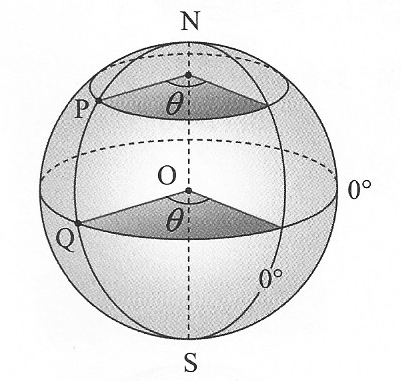
\includegraphics[scale=1.4]{longitude.png}
    \end{center}

    \subsection*{Latitude and Parallels of Latitude}

    The lines of latitude are the circles that are perpendicular to the plane that
    passes through the north and south poles. The \emph{equator} is the one and
    only great circle among the parallels of latitude.

    \begin{center}
        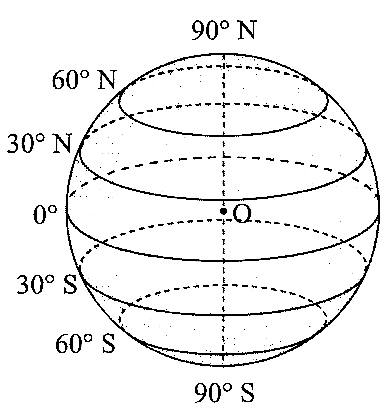
\includegraphics[scale=1.3]{latitude}
    \end{center}

    The angle between the equator and the line of latitude that passes through the
    point $P$ is called the \emph{latitude of $P$}. There are 180 degrees of
    latitude ($+90^\circ$ northward and $-90^\circ$ southward). The equator divides
    the world into the Northern Hemisphere and the Southern Hemisphere.

    \begin{center}
        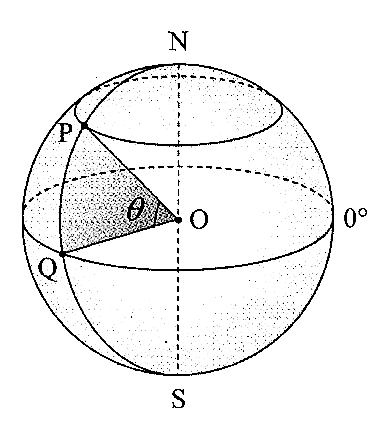
\includegraphics[scale=1.3]{latitude 2.png}
    \end{center}

    \subsection{Practice 3}

    \begin{enumerate}
        \item In the diagram below, $NGS$ is the prime meridian, $O$ is the centre of the
              earth. Find the longitude of locations $P$, $Q$, $R$ and $T$.
              \begin{center}
                  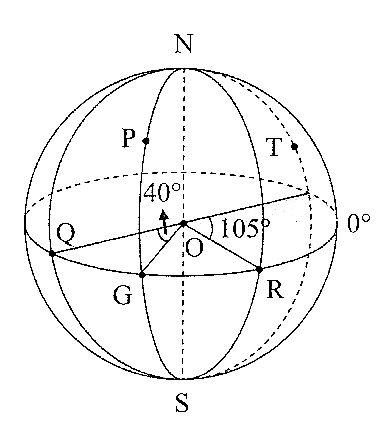
\includegraphics[scale=1.3]{p3q1.png}
              \end{center}
              \sol{}
              \begin{flalign*}
                  \text{Lon. } P & = 0^\circ     \\
                  \text{Lon. } Q & = 40^\circ W  \\
                  \text{Lon. } R & = 35^\circ E  \\
                  \text{Lon. } T & = 140^\circ E
              \end{flalign*}

        \item In the diagram below, $O$ is the centre of the earth, location $A$ and $B$ are
              on the equator. Find the location of $P$, $Q$, $R$ and $T$.
              \begin{center}
                  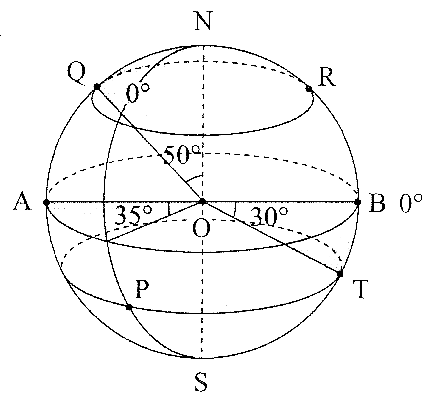
\includegraphics[scale=1.3]{p3q2.png}
              \end{center}
              \sol{}
              \begin{flalign*}
                  \text{Lon. } P & = 0^\circ                 \\
                  \text{Lat. } P & = 30^\circ S              \\
                  \therefore \ P & (30^\circ S, 0^\circ)     \\
                  \\
                  \text{Lon. } Q & = 35^\circ W              \\
                  \text{Lat. } Q & = 40^\circ N              \\
                  \therefore \ Q & (40^\circ N, 35^\circ W)  \\
                  \\
                  \text{Lon. } R & = 145^\circ E             \\
                  \text{Lat. } R & = 40^\circ N              \\
                  \therefore \ R & (40^\circ N, 145^\circ E) \\
                  \\
                  \text{Lon. } T & = 145^\circ E             \\
                  \text{Lat. } T & = 30^\circ S              \\
                  \therefore \ T & (30^\circ S, 145^\circ E)
              \end{flalign*}
    \end{enumerate}

    \subsection*{Radius of the Parallel of Latitude}

    Let $R$ be the radius of the earth, $r$ be the radius of latitude $\theta$,
    then $r = R \cos \theta$.
    \begin{center}
        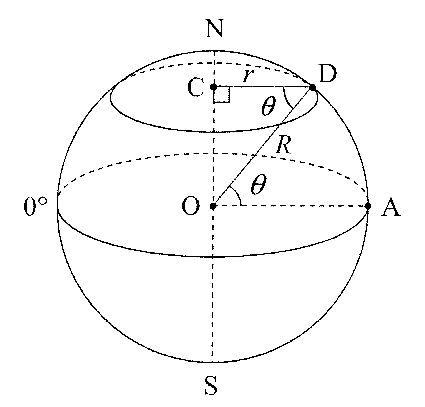
\includegraphics[scale=1.3]{radius of latitude.png}
    \end{center}

    \subsection*{Nautical Miles}

    The arc length corresponding to $1'$ ($=\frac{1}{60}^\circ$) of the great
    circle on earth is called a \emph{nautical mile} ($1$\emph{NM}), that is,
    $1\text{\emph{NM}} = \frac{1}{60 \times 360} \times 2\pi \times 6370km =
        1.853km$.

    \subsection*{Time Difference and Longitude}

    The time is calculated by the rotation of the earth around its axis. The earth
    rotates around its axis from west to east once in $24h$. That is, the earth
    rotates $15^\circ$ in $1h$. Thus, the time difference between two locations on
    the earth is equal to the difference of their longitudes. Thus, the time
    difference is $1hr$ per $15^\circ$ of longitude difference.

    \begin{enumerate}[listparindent=1.5em]
        \item \textbf{Local Time}\\
              The local time is the time at a location on the earth. The local time for any location on the same line of longitude is the same.
        \item \textbf{Standard Time}\\
              Back in the year $1844$, International Meridian Conference was held in Washington DC. The conference decided to divide the world into 24 time zones based on the Greenwich Meridian, called the \emph{Greenwich Meridian Time (GMT)}. There is zero time offset $7.5^\circ$ eastward and $7.5^\circ$ westward of the Greenwich Meridian. The time offset is $1hr$ per $15^\circ$ of longitude difference. All places in the same time zone share the same local time with the location located on the line of longitude that passes through the centre of the time zone, called the \emph{standard time} or \emph{zone time}.

              \indent When entering a new time zone from the east, the local time is advanced by
              $1hr$ per $15^\circ$ of longitude difference. When entering a new time zone
              from the west, the local time is delayed by $1hr$ per $15^\circ$ of longitude
              difference.
    \end{enumerate}
\end{multicols}
\begin{center}
    \makebox[\textwidth]{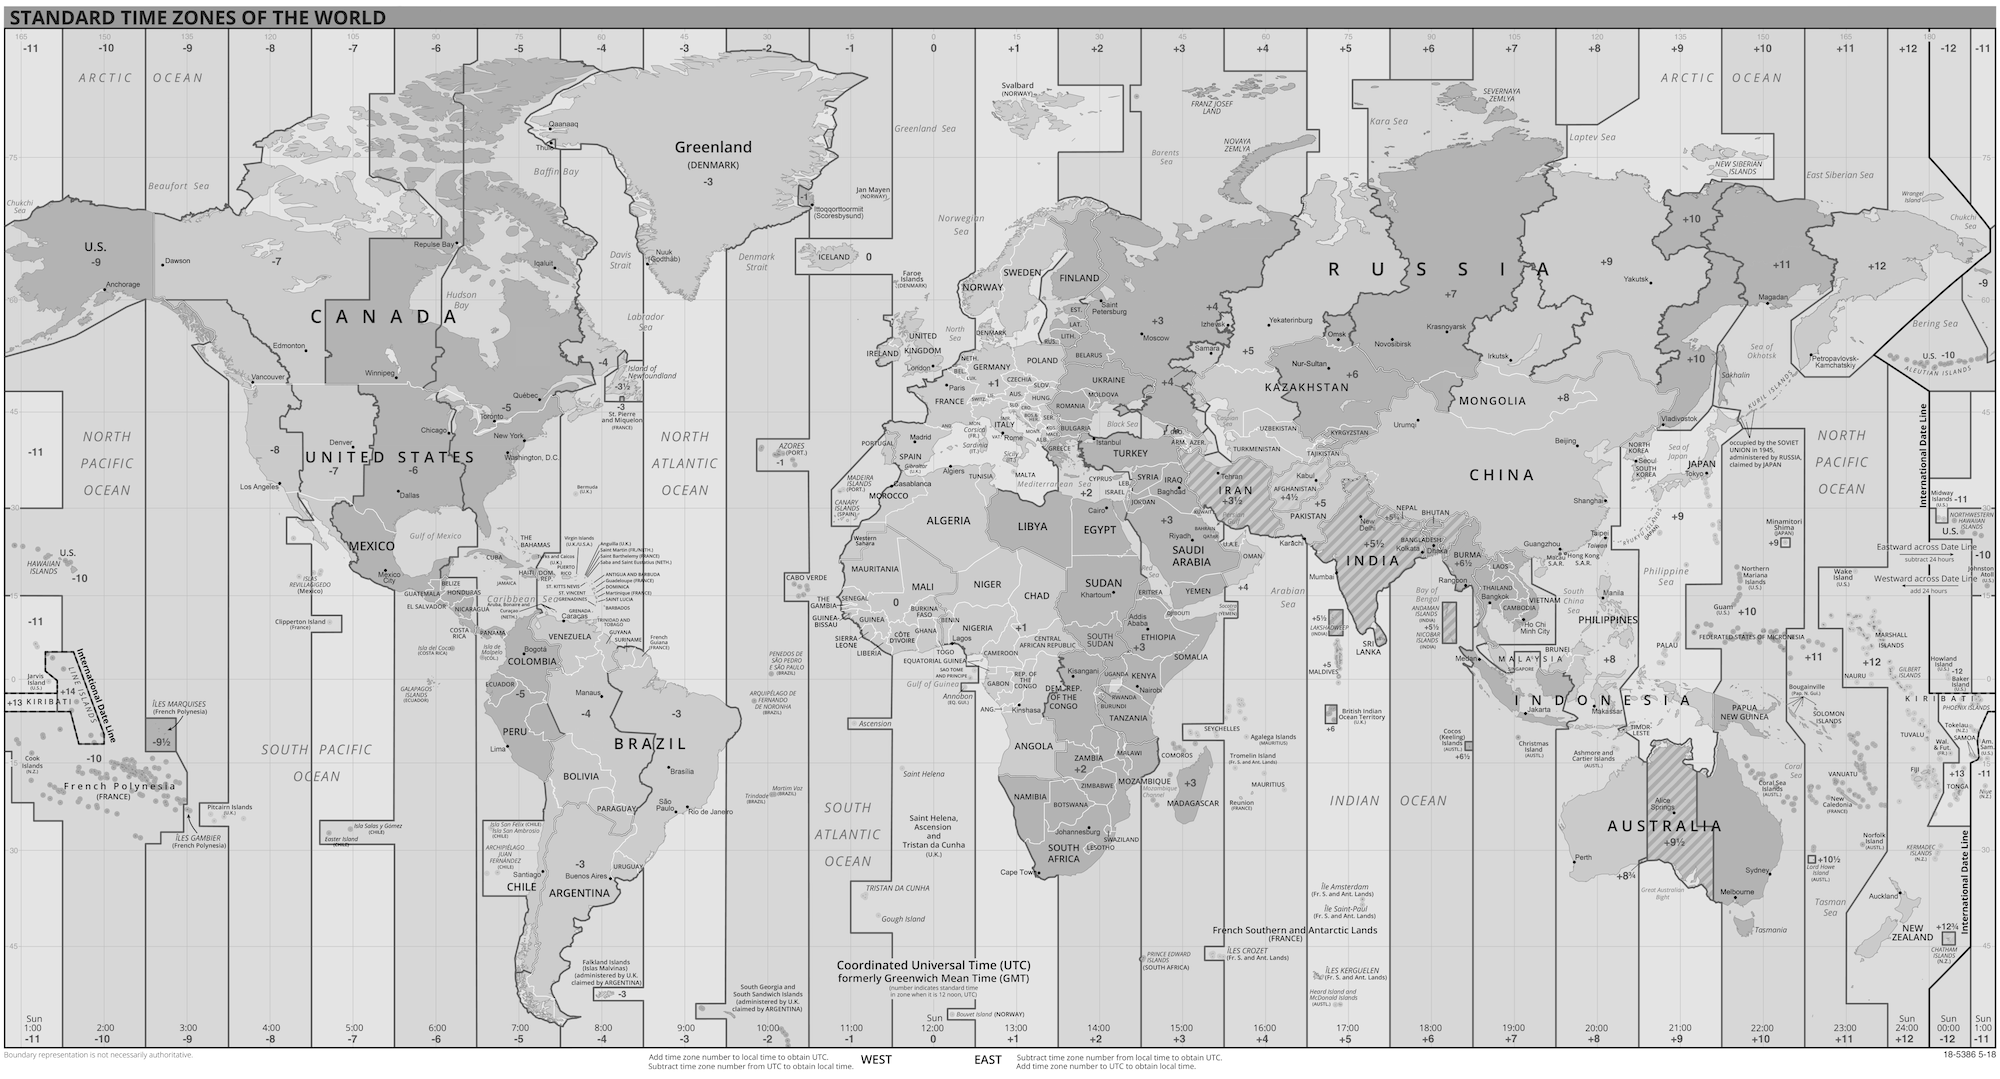
\includegraphics[scale=0.42]{timezone.png}}
\end{center}
\begin{multicols}{2}
    \section{Distance of Two Locations on the Same Line of Longitude}

    The distance of two location on the same line of longitude is the arc length
    corresponding to the difference of their latitudes. Given two location $P$ and
    $Q$ on the same line of longitude, according to the definition of nautical
    mile, the distance between $P$ and $Q$ can be acquired by the arc length of
    $PQ$. That is, $\overset{\frown}{PQ} = \theta \times 60$\emph{NM}, where
    $\theta$ is the difference of their latitudes.

    \begin{center}
        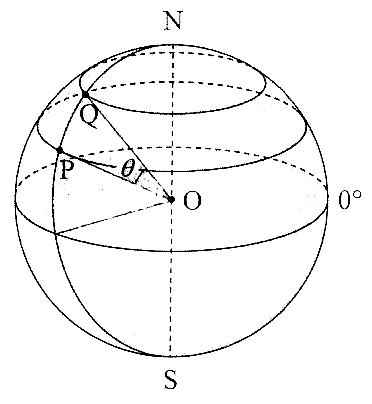
\includegraphics[scale=1.4]{longitude difference.png}
    \end{center}

    \subsection{Practice 4}

    \begin{enumerate}
        \item Given that location $A$ and $B$ are on the same line of longitude. Based on the
              following longitude, find the distance between $A$ and $B$ (Express your answer
              in nautical miles):
              \begin{enumerate}
                  \item $A(58^\circ N)$, $B(75^\circ N)$
                        \sol{}
                        \begin{flalign*}
                            \overset{\frown}{AB} & = (75^\circ - 58^\circ) \times 60\text{\emph{NM}} \\
                                                 & = 17 \times 60\text{\emph{NM}}                    \\
                                                 & = 1020\text{\emph{NM}}
                        \end{flalign*}

                  \item $A(0^\circ)$, $B(42^\circ S)$
                        \sol{}
                        \begin{flalign*}
                            \overset{\frown}{AB} & = (42^\circ - 0^\circ) \times 60\text{\emph{NM}} \\
                                                 & = 42 \times 60\text{\emph{NM}}                   \\
                                                 & = 2520\text{\emph{NM}}
                        \end{flalign*}

                  \item $A(43^\circ N)$, $B(38^\circ S)$
                        \sol{}
                        \begin{flalign*}
                            \overset{\frown}{AB} & = (38^\circ + 43^\circ) \times 60\text{\emph{NM}} \\
                                                 & = 81 \times 60\text{\emph{NM}}                    \\
                                                 & = 4860\text{\emph{NM}}
                        \end{flalign*}
              \end{enumerate}
        \item Given that location $P$ and $Q$ are on the same line of longitude. The distane
              between two locations is $1000$\emph{NM}, $P$ is located at $7^\circ 30'$ north
              of the equator. Based on the following criteria, find the latitude of $Q$:
              \begin{flalign*}
                  \overset{\frown}{PQ} & = \theta \times 60 \\
                  1000                 & = \theta \times 60 \\
                  \theta               & = \frac{1000}{60}  \\
                                       & = 16^\circ40'
              \end{flalign*}
              \begin{enumerate}
                  \item $Q$ is located at the north of $P$
                        \sol{}
                        \begin{flalign*}
                            \text{Lat. } Q & = (7^\circ 30' + 16^\circ 40')N \\
                                           & = 24^\circ 10'N
                        \end{flalign*}

                  \item $Q$ is located at the south of $P$
                        \sol{}
                        \begin{flalign*}
                            \text{Lat. } Q & = |7^\circ 30' - 16^\circ 40'|S \\
                                           & = 9^\circ 10'S
                        \end{flalign*}
              \end{enumerate}
    \end{enumerate}

    \subsection{Exercise 17.5}

    \begin{enumerate}
        \item Given that $A$ and $B$ are on the same line of longitude. Based on the
              following difference of latitude of two locations, find the distance between
              $A$ and $B$ (Express your answer in nautical miles):
              \begin{enumerate}
                  \item $\theta = 39^\circ$
                        \sol{}
                        \begin{flalign*}
                            \overset{\frown}{AB} & = 39 \times 60\text{\emph{NM}} \\
                                                 & = 2340\text{\emph{NM}}
                        \end{flalign*}

                  \item $\theta = 80^\circ 30'$
                        \sol{}
                        \begin{flalign*}
                            \overset{\frown}{AB} & = (80^\circ 30') \times 60\text{\emph{NM}} \\
                                                 & = 4830\text{\emph{NM}}
                        \end{flalign*}

                  \item $\theta = 64^\circ 20'$
                        \sol{}
                        \begin{flalign*}
                            \overset{\frown}{AB} & = (64^\circ 20') \times 60\text{\emph{NM}} \\
                                                 & = 3860\text{\emph{NM}}
                        \end{flalign*}
              \end{enumerate}

        \item Given that $A$ and $B$ are on the same line of longitude. Based on the
              following distance between two locations, find the difference of latitude of
              $A$ and $B$ (Round your answer to the nearest minute):
              \begin{enumerate}
                  \item $700$\emph{NM}
                        \sol{}
                        \begin{flalign*}
                            \overset{\frown}{AB} & = \theta \times 60 \\
                            700                  & = \theta \times 60 \\
                            \theta               & = \frac{700}{60}   \\
                                                 & = 11^\circ 40'
                        \end{flalign*}

                  \item $318$\emph{NM}
                        \sol{}
                        \begin{flalign*}
                            \overset{\frown}{AB} & = \theta \times 60 \\
                            318                  & = \theta \times 60 \\
                            \theta               & = \frac{318}{60}   \\
                                                 & = 5^\circ 18'
                        \end{flalign*}

                  \item $3450$\emph{NM}
                        \sol{}
                        \begin{flalign*}
                            \overset{\frown}{AB} & = \theta \times 60 \\
                            3450                 & = \theta \times 60 \\
                            \theta               & = \frac{3450}{60}  \\
                                                 & = 57^\circ 30'
                        \end{flalign*}
              \end{enumerate}

        \item Find the distance between two locations along the same line of longitude:
              \begin{enumerate}
                  \item $A(21^\circ S, 110^\circ E)$, $B(33^\circ S, 110^\circ E)$
                        \sol{}
                        \begin{flalign*}
                            \overset{\frown}{AB} & = (33^\circ - 21^\circ) \times 60\text{\emph{NM}} \\
                                                 & = 12 \times 60\text{\emph{NM}}                    \\
                                                 & = 720\text{\emph{NM}}
                        \end{flalign*}

                  \item $X(38^\circ N, 40^\circ W)$, $Y(19^\circ N, 40^\circ W)$
                        \sol{}
                        \begin{flalign*}
                            \overset{\frown}{XY} & = (38^\circ - 19^\circ) \times 60\text{\emph{NM}} \\
                                                 & = 19 \times 60\text{\emph{NM}}                    \\
                                                 & = 1140\text{\emph{NM}}
                        \end{flalign*}

                  \item $E(34^\circ 45' S, 80^\circ E)$, $F(0^\circ, 80^\circ E)$
                        \sol{}
                        \begin{flalign*}
                            \overset{\frown}{EF} & = (34^\circ 45' - 0^\circ) \times 60\text{\emph{NM}} \\
                                                 & = 34^\circ 45' \times 60\text{\emph{NM}}             \\
                                                 & = 2085\text{\emph{NM}}
                        \end{flalign*}

                  \item $P(18^\circ 15' N, 90^\circ W)$, $Q(43^\circ 30' N, 90^\circ W)$
                        \sol{}
                        \begin{flalign*}
                            \overset{\frown}{PQ} & = (43^\circ 30' - 18^\circ 15') \times 60\text{\emph{NM}} \\
                                                 & = 25^\circ 15' \times 60\text{\emph{NM}}                  \\
                                                 & = 1515\text{\emph{NM}}
                        \end{flalign*}

                  \item $T(15^\circ 30' N, 120^\circ E)$, $M(24^\circ 30' S, 120^\circ E)$
                        \sol{}
                        \begin{flalign*}
                            \overset{\frown}{TM} & = (24^\circ 30' + 15^\circ 30') \times 60\text{\emph{NM}} \\
                                                 & = 40^\circ \times 60\text{\emph{NM}}                      \\
                                                 & = 2400\text{\emph{NM}}
                        \end{flalign*}
              \end{enumerate}

        \item Location $X$ and $Y$ are on the same line of longitude, the distane between
              them is $400$\emph{NM}. Find the difference of latitude of $X$ and $Y$. \sol{}
              \begin{flalign*}
                  \overset{\frown}{XY} & = \theta \times 60 \\
                  400                  & = \theta \times 60 \\
                  \theta               & = \frac{400}{60}   \\
                                       & = 6^\circ 40'
              \end{flalign*}

        \item Location $P$ and $Q$ are on the same line of longitude, and their distance
              along the line of longitude is $600$\emph{NM}, find the difference between
              their latitude. \sol{}
              \begin{flalign*}
                  \overset{\frown}{PQ} & = \theta \times 60           \\
                  \frac{600}{1.853}    & = \theta \times 60           \\
                  \theta               & = \frac{600}{1.853\times 60} \\
                                       & \approx 5.24^\circ
              \end{flalign*}

        \item $X$ city and $Y$ city are on the same line of longitude, the latitude of $X$ city is $2^\circ 15'$ north of the equator, the latitude of $Y$ city is $6^\circ$ north of the equator. Find the distance between $X$ city and $Y$ city (Express your answer in kilometers).
              \sol{}
              \begin{flalign*}
                  \overset{\frown}{XY} & = (6^\circ - 2^\circ 15') \times 60\text{\emph{NM}} \\
                                       & = 3^\circ 45' \times 60\text{\emph{NM}}             \\
                                       & = 225\text{\emph{NM}}                               \\
                                       & = 225 \times 1.853km                                \\
                                       & = 416.93km
              \end{flalign*}

        \item A plane is flying $1000km$ due north from airport $A(15^\circ N, 115^\circ E)$
              to airport $B$. Find the longitude and latitude of airport $B$. \sol{}
              \begin{flalign*}
                  \overset{\frown}{AB} & = \theta \times 60\text{\emph{NM}} \\
                  \frac{1000}{1.853}   & = \theta \times 60                 \\
                  \theta               & = \frac{1000}{1.853\times 60}      \\
                                       & = 9^\circ
                  \\
                  \text{Lat.} B        & = (15^\circ + 9^\circ)N            \\
                                       & = 24^\circ N                       \\
                  \\
                  \therefore\ B        & (24^\circ N, 115^\circ E)
              \end{flalign*}

        \item A plane is flying $1500km$ due south from airport $A(5^\circ N, 100^\circ E)$
              to airport $B$. Find the longitude and latitude of airport $B$. \sol{}
              \begin{flalign*}
                  \overset{\frown}{AB} & = \theta \times 60\text{\emph{NM}} \\
                  \frac{1500}{1.853}   & = \theta \times 60                 \\
                  \theta               & = \frac{1500}{1.853\times 60}      \\
                                       & = 13^\circ 30'                     \\
                  \text{Lat.} B        & = |5^\circ - 13^\circ 30'|S        \\
                                       & = 8^\circ 30' S                    \\
                  \\
                  \therefore\ B        & (8^\circ 30' S, 100^\circ E)
              \end{flalign*}

        \item Find the distance from $A(18^\circ 30' S)$ to the north pole along the same
              line of longitude. \sol{}
              \begin{flalign*}
                  \overset{\frown}{AN} & = (90^\circ + 18^\circ 30') \times 60\text{\emph{NM}} \\
                                       & = 108^\circ 30' \times 60\text{\emph{NM}}             \\
                                       & = 6510\text{\emph{NM}}
              \end{flalign*}

        \item The distance between location $C$ and $D$ is $700$\emph{NM}, $C$ is located at
              the south of $D$. Assume that $C$ is located at $5^\circ 30'$ north of the
              equator. Find the latitude of $D$. \sol{}
              \begin{flalign*}
                  \overset{\frown}{CD}      & = \theta \times 60\text{\emph{NM}} \\
                  700                       & = \theta \times 60                 \\
                  \theta                    & = \frac{700}{60}                   \\
                                            & = 11^\circ 40'                     \\
                  \\
                  \therefore\ \text{Lat.} D & = (35^\circ 30' + 11^\circ 40')N   \\
                                            & = 47^\circ 10' N
              \end{flalign*}

        \item A plane takes off from $P(60^\circ N, 60^\circ E)$ and flies pass north pole
              along the great circle route to $Q(50^\circ N, 120^\circ W)$. Find the flying
              distance. \sol{}
              \begin{flalign*}
                  \overset{\frown}{PN} & = (90^\circ - 60^\circ) \times 60\text{\emph{NM}} \\
                                       & = 30^\circ \times 60\text{\emph{NM}}              \\
                                       & = 1800\text{\emph{NM}}                            \\
                  \overset{\frown}{NQ} & = (90^\circ - 50^\circ) \times 60\text{\emph{NM}} \\
                                       & = 40^\circ \times 60\text{\emph{NM}}              \\
                                       & = 2400\text{\emph{NM}}                            \\
                  \overset{\frown}{PQ} & = \overset{\frown}{PN} + \overset{\frown}{NQ}     \\
                                       & = 1800 + 2400                                     \\
                                       & = 4200\text{\emph{NM}}
              \end{flalign*}

        \item A ship sails from $P(50^\circ S, 160^\circ E)$ due north to another port
              $Q(30^\circ N, 160^\circ E)$. The sailing time is 10 days. Find the average
              speed of the ship. (Express your answer in \emph{NM}$/hr$) \sol{}
              \begin{flalign*}
                  \overset{\frown}{PQ} & = (30^\circ + 50^\circ) \times 60\text{\emph{NM}} \\
                                       & = 80^\circ \times 60\text{\emph{NM}}              \\
                                       & = 4800\text{\emph{NM}}                            \\
                  \text{Average speed} & = \frac{\overset{\frown}{PQ}}{10\times 24}        \\
                                       & = 20\text{\emph{NM}}/hr
              \end{flalign*}

        \item Given that $PQ$ is the diameter of the parallel of latitude $35^\circ S$. A
              plane takes off from location $P$, flies pass the south pole along the line of
              longitude, and lands at location $Q$ after $13hrs 40mins$. Find the average
              speed of the plane for the whole flight duration. (Express your answer in
              \emph{NM}$/hr$) \sol{}
              \begin{flalign*}
                  \overset{\frown}{PQ} & = 2(90^\circ - 35^\circ) \times 60\text{\emph{NM}} \\
                                       & = 110^\circ \times 60\text{\emph{NM}}              \\
                                       & = 6600\text{\emph{NM}}                             \\
                  \text{Average speed} & = \frac{\overset{\frown}{PQ}}{13\frac{40}{60}hr}   \\
                                       & = \frac{6600NM}{\frac{41}{3}hr}                    \\
                                       & = 482.93\text{\emph{NM}}/hr
              \end{flalign*}
    \end{enumerate}

    \section{Distance of Two Locations on the Same Parallel of Latitude}

    The distance between two locations on the same parallel of latitude is the arc
    length on the parallel of latitude corresponding to the difference of their
    longitudes.

    \begin{center}
        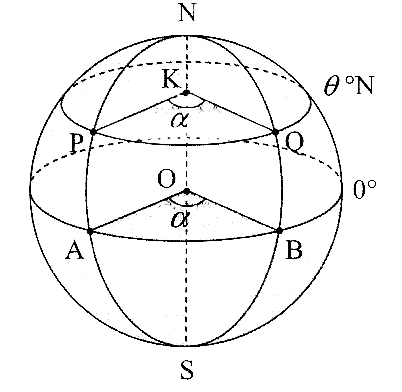
\includegraphics[scale=1.4]{latitude difference.png}
    \end{center}

    In the diagram above, $P$ and $Q$ are on the same parallel of latitude
    $\theta$, their difference of latitude is $\alpha$. $A$ and $B$ are locations
    on the equator.

    Given that $\angle PKQ = \angle AOB = \alpha$. Let $R$ be the radius of the
    earth, $r$ be the radius of the parallel of latitude.

    \begin{flalign*}
        \frac{\overset{\frown}{PQ}}{\overset{\frown}{AB}} & = \frac{\frac{\alpha}{360^\circ} \times 2\pi r}{\frac{\alpha}{360^\circ} \times 2\pi R} \\
                                                          & = \frac{r}{R}                                                                           \\
    \end{flalign*}

    From the radius of the the parallel of latitude $r = R \cos R$, we have
    $\frac{r}{R} = \cos \theta$.
    \begin{flalign*}
        \therefore \frac{\overset{\frown}{PQ}}{\overset{\frown}{AB}} & = \cos \theta                                             \\
        \overset{\frown}{PQ}                                         & = \overset{\frown}{AB} \times \cos \theta                 \\
                                                                     & = \alpha \times 60 \times \cos \theta \text{\emph{NM} or} \\
                                                                     & = \alpha \times 60 \times \cos \theta \times 1.853km
    \end{flalign*}

    \subsection{Practice 5}

    \begin{enumerate}
        \item Fidn the distance of the following pairs of location on the same parallel of
              latitude (Express your answer in nautical miles):
              \begin{enumerate}
                  \item $P(80^\circ N, 105^\circ W), Q(80^\circ N, 48^\circ W)$
                        \sol{}
                        \begin{flalign*}
                            \overset{\frown}{PQ} & = (105 - 48) \times 60 \times \cos 80^\circ \\
                                                 & = 57 \times 60 \times \cos 80^\circ         \\
                                                 & = 593.88 \text{\emph{NM}}
                        \end{flalign*}

                  \item $M(50^\circ S, 48^\circ E), N(50^\circ S, 100^\circ E)$
                        \sol{}
                        \begin{flalign*}
                            \overset{\frown}{MN} & = (100 - 48) \times 60 \times \cos 50^\circ \\
                                                 & = 52 \times 60 \times \cos 50^\circ         \\
                                                 & = 2005.50 \text{\emph{NM}}
                        \end{flalign*}

                  \item $X(40^\circ N, 28^\circ 15' E), Y(40^\circ N, 42^\circ 45' W)$
                        \sol{}
                        \begin{flalign*}
                            \overset{\frown}{XY} & = (28.25 + 42.75) \times 60 \times \cos 40^\circ \\
                                                 & = 71 \times 60 \times \cos 40^\circ              \\
                                                 & = 3263.35 \text{\emph{NM}}
                        \end{flalign*}

                  \item $K(20^\circ S, 160^\circ E), L(20^\circ S, 140^\circ W)$
                        \sol{}
                        \begin{flalign*}
                            \overset{\frown}{KL} & = (360 - 160 - 140) \times 60 \times \cos 20^\circ \\
                                                 & = 60 \times 60 \times \cos 20^\circ                \\
                                                 & = 3382.90 \text{\emph{NM}}
                        \end{flalign*}
              \end{enumerate}

        \item Given that $A$ is located at the west of $B(46^\circ N, 72^\circ W)$ with a
              distance of $2350$\emph{NM}. Find the longitude and latitude of $A$. \sol{}
              \begin{flalign*}
                  \overset{\frown}{AB} & = \alpha \times 60 \times \cos 46 \\
                  2350                 & = \alpha \times 60 \times \cos 46 \\
                  \alpha               & = \frac{2350}{60 \times \cos 46}  \\
                  \alpha               & = 56^\circ 23'                    \\
                  \text{Lon.} A        & = (72^\circ + 56^\circ 23')W      \\
                                       & = 128^\circ 23'W                  \\
                  \\
                  \therefore\ A        & (46^\circ N, 128^\circ 23'W)
              \end{flalign*}
    \end{enumerate}
    \subsection{Exercise 17.6}
    \begin{enumerate}
        \item Find the distance of the following pairs of location on the same parallel of
              latitude (Express your answer in nautical miles):
              \begin{enumerate}
                  \item $P(45^\circ S, 20^\circ E), Q(45^\circ S, 100^\circ E)$
                        \sol{}
                        \begin{flalign*}
                            \overset{\frown}{PQ} & = (100 - 20) \times 60 \times \cos 45^\circ \\
                                                 & = 80 \times 60 \times \cos 45^\circ         \\
                                                 & = 3394.11 \text{\emph{NM}}
                        \end{flalign*}

                  \item $M(36^\circ N, 45^\circ W), N(36^\circ N, 105^\circ W)$
                        \sol{}
                        \begin{flalign*}
                            \overset{\frown}{MN} & = (105 - 45) \times 60 \times \cos 36^\circ \\
                                                 & = 60 \times 60 \times \cos 36^\circ         \\
                                                 & = 2192.46 \text{\emph{NM}}
                        \end{flalign*}

                  \item $A(80^\circ S, 130^\circ E), B(80^\circ S, 165^\circ E)$
                        \sol{}
                        \begin{flalign*}
                            \overset{\frown}{AB} & = (165 - 130) \times 60 \times \cos 80^\circ \\
                                                 & = 35 \times 60 \times \cos 80^\circ          \\
                                                 & = 364.66 \text{\emph{NM}}
                        \end{flalign*}

                  \item $K(70^\circ N, 40^\circ E), L(70^\circ N, 20^\circ W)$
                        \sol{}
                        \begin{flalign*}
                            \overset{\frown}{KL} & = (40 + 20) \times 60 \times \cos 70^\circ \\
                                                 & = 60 \times 60 \times \cos 70^\circ        \\
                                                 & = 1231.27 \text{\emph{NM}}
                        \end{flalign*}

                  \item $T(0^\circ, 128^\circ W), M(0^\circ, 120^\circ E)$
                        \sol{}
                        \begin{flalign*}
                            \overset{\frown}{TM} & = (360 - 128 - 120) \times 60 \times \cos 0^\circ \\
                                                 & = 112 \times 60 \times \cos 0^\circ               \\
                                                 & = 6720 \text{\emph{NM}}
                        \end{flalign*}
              \end{enumerate}
        \item Based on the following distances of location $P$ and $Q$ and the longitude and
              latitude of $P$, find the longitude and latitude of $Q$:
              \begin{enumerate}
                  \item $PQ = 800$\emph{NM}, $Q$ is located at the west of $P(50^\circ S, 100^\circ W)$
                        \sol{}
                        \begin{flalign*}
                            \overset{\frown}{PQ} & = \alpha \times 60 \times \cos 50^\circ \\
                            800                  & = \alpha \times 60 \times \cos 50^\circ \\
                            \alpha               & = \frac{800}{60 \times \cos 50^\circ}   \\
                            \alpha               & = 20^\circ 45'                          \\
                            \text{Lon.} Q        & = (100^\circ - 20^\circ 45')W           \\
                                                 & = 120^\circ 45'W                        \\
                            \\
                            \therefore\ Q        & (50^\circ S, 120^\circ 45'W)
                        \end{flalign*}

                  \item $PQ = 3400$\emph{NM}, $Q$ is located at the east of $P(35^\circ N, 68^\circ E)$
                        \sol{}
                        \begin{flalign*}
                            \overset{\frown}{PQ} & = \alpha \times 60 \times \cos 35^\circ \\
                            3400                 & = \alpha \times 60 \times \cos 35^\circ \\
                            \alpha               & = \frac{3400}{60 \times \cos 35^\circ}  \\
                            \alpha               & = 69^\circ 11'                          \\
                            \text{Lon.} Q        & = (68^\circ + 69^\circ 11')E            \\
                                                 & = 137^\circ 11'E                        \\
                            \\
                            \therefore\ Q        & (35^\circ N, 137^\circ 11'E)
                        \end{flalign*}

                  \item $PQ = 1450km$, $Q$ is located at the east of $P(42^\circ N, 15^\circ W)$
                        \sol{}
                        \begin{flalign*}
                            \overset{\frown}{PQ} & = \alpha \times 60 \times \cos 42^\circ             \\
                            \frac{1450}{1.853}   & = \alpha \times 60 \times \cos 42^\circ             \\
                            \alpha               & = \frac{1450}{1.853 \times 60 \times \cos 42^\circ} \\
                            \alpha               & = 17^\circ 33'                                      \\
                            \text{Lon.} Q        & = |15^\circ - 17^\circ 33'|E                        \\
                                                 & = 2^\circ 33'E                                      \\
                            \\
                            \therefore\ Q        & (42^\circ N, 2^\circ 33'E)
                        \end{flalign*}
              \end{enumerate}

        \item Given that two places are on the parallel of latitude $60^\circ$ north to the
              equator, and their difference of longitude is $160^\circ$. Find the distance of
              the two places. (Express your answer in kilometers) \sol{}

              Let the two places are $A$ and $B$.
              \begin{flalign*}
                  \overset{\frown}{AB} & = 160 \times 60 \times \cos 60^\circ \\
                                       & = 4800 \text{\emph{NM}}              \\
                                       & = 4800 \times 1.853km                \\
                                       & = 8894.4 \text{\emph{km}}
              \end{flalign*}

        \item City $A$ and $B$ are on the parallel of latitude $5^\circ 30'$ north to the
              equator, their longitude are $100^\circ 15' E$ and $103^\circ E$ respectively.
              Find the distance between two cities along the parallel of latitude. \sol{}
              \begin{flalign*}
                  \overset{\frown}{AB} & = (103^\circ - 100^\circ 15') \times 60 \times \cos 5^\circ 30' \\
                                       & = 2^\circ45' \times 60 \times \cos 5^\circ 30'                  \\
                                       & = 164.24 \text{\emph{NM}}
              \end{flalign*}

        \item Find the circumference of the parallel of latitude $35^\circ 30' S$. \sol{}
              \begin{flalign*}
                  C & = 360 \times 60 \times \cos 35^\circ 30' \\
                    & = 17584.90 \text{\emph{NM}}
              \end{flalign*}

        \item Find the radius of the parallel of latitude $60^\circ N$. \sol{}
              \begin{flalign*}
                  r & = \frac{360 \times 60 \times \cos 60^\circ}{2 \pi} \\
                    & = 1718.87 \text{\emph{NM}}                         \\
                    & = 1718.87 \times 1.853 \text{\emph{km}}            \\
                    & = 3185.10 \text{\emph{km}}
              \end{flalign*}

        \item A ship set sail from $P(20^\circ E)$ and sail $600$\emph{NM} due east along
              $42^\circ N$ parallel of latitude. Find the longitude and latitude of the
              destination. \sol{}

              Let the destination is $Q$.
              \begin{flalign*}
                  \overset{\frown}{PQ} & = \alpha \times 60 \times \cos 42^\circ \\
                  600                  & = \alpha \times 60 \times \cos 42^\circ \\
                  \alpha               & = \frac{600}{60 \times \cos 42^\circ}   \\
                                       & = 13^\circ 27'                          \\
                  \text{Lon.} Q        & = (20^\circ + 13^\circ 27')E            \\
                                       & = 33^\circ 27'E                         \\
                  \\
                  \therefore\ Q        & (42^\circ N, 33^\circ 27'E)
              \end{flalign*}

        \item A ship sails from port $P(48^\circ N, 12^\circ W)$ $1000$\emph{NM} due west to
              another port $Q$, find the longitude and latitude of $Q$. \sol{}
              \begin{flalign*}
                  \overset{\frown}{PQ} & = \alpha \times 60 \times \cos 48^\circ \\
                  1000                 & = \alpha \times 60 \times \cos 48^\circ \\
                  \alpha               & = \frac{1000}{60 \times \cos 48^\circ}  \\
                                       & = 24^\circ 54'                          \\
                  \text{Lon.} Q        & = (12^\circ - 24^\circ 54')W            \\
                                       & = 36^\circ 54'W                         \\
                  \\
                  \therefore\ Q        & (48^\circ N, 36^\circ 54'W)
              \end{flalign*}

        \item Given that $A$ is located at the east of Paris$(49^\circ N, 2^\circ 30' E)$
              with a distance of $2200km$. Find the longitude and latitude of $A$. \sol{}
              \begin{flalign*}
                  \overset{\frown}{PA} & = \alpha \times 60 \times \cos 49^\circ             \\
                  \frac{2000}{1.853}   & = \alpha \times 60 \times \cos 49^\circ             \\
                  \alpha               & = \frac{2200}{1.853 \times 60 \times \cos 49^\circ} \\
                                       & = 30^\circ 10'                                      \\
                  \text{Lon.} A        & = (2^\circ 30' + 30^\circ 10')E                     \\
                                       & = 32^\circ 40'E                                     \\
                  \\
                  \therefore\ A        & (49^\circ N, 32^\circ 40'E)
              \end{flalign*}

        \item A plane flies from $X(40^\circ N, 75^\circ W)$ $9265km$ due east to $Y$, find
              the longitude and latitude of $Y$. \sol{}
              \begin{flalign*}
                  \overset{\frown}{XY} & = \alpha \times 60 \times \cos 40^\circ             \\
                  \frac{9265}{1.853}   & = \alpha \times 60 \times \cos 40^\circ             \\
                  \alpha               & = \frac{9265}{1.853 \times 60 \times \cos 40^\circ} \\
                                       & = 108^\circ 47'                                     \\
                  \text{Lon.} Y        & = |75^\circ - 108^\circ 47'|E                       \\
                                       & = 33^\circ 47'E                                     \\
                  \\
                  \therefore\ Y        & (40^\circ N, 33^\circ 47'E)
              \end{flalign*}

        \item A plane flies from Berlin$(52^\circ 30' N, 13^\circ 30' E)$ due west $1853km$
              to $P$, find the longitude and latitude of $P$. \sol{}
              \begin{flalign*}
                  \overset{\frown}{BP} & = \alpha \times 60 \times \cos 52^\circ 30'             \\
                  \frac{1853}{1.853}   & = \alpha \times 60 \times \cos 52^\circ 30'             \\
                  \alpha               & = \frac{1853}{1.853 \times 60 \times \cos 52^\circ 30'} \\
                                       & = 27^\circ 23'                                          \\
                  \text{Lon.} P        & = |13^\circ 30' - 27^\circ 23'|W                        \\
                                       & = 13^\circ 53'W                                         \\
                  \\
                  \therefore\ P        & (52^\circ 30' N, 13^\circ 53'W)
              \end{flalign*}

        \item Given that the earth takes $24hrs$ to rotate once. Find the speed of Kuala
              Lumpur$(3^\circ 15' N, 102^\circ E)$ to rotate once. (Express your answer in
              \emph{NM}$/hr$) \sol{}
              \begin{flalign*}
                  \text{Speed} & = \frac{(360 \times 60 \times \cos 3^\circ 15')\text{\emph{NM}}}{24hr} \\
                               & = 898.55 \text{\emph{NM}}/hr
              \end{flalign*}

        \item Given that the longitude of $P$ and $Q$ are $50^\circ W$ and $110^\circ W$
              respectively. If $P$ and $Q$ both located at the west of $R(55^\circ S)$ and
              $PR = PQ$, find:
              \begin{enumerate}
                  \item The longitude of $R$. \sol{}
                        \begin{flalign*}
                            \overset{\frown}{PQ} & = (110^\circ - 50^\circ) \times 60 \times \cos 55^\circ \\
                                                 & = 2064.875 \text{\emph{NM}}                             \\
                            \overset{\frown}{PR} & = \alpha \times 60 \times \cos 55^\circ                 \\
                            2064.875             & = \alpha \times 60 \times \cos 55^\circ                 \\
                            \alpha               & = \frac{2064.875}{60 \times \cos 55^\circ}              \\
                                                 & = 60^\circ                                              \\
                            \text{Lon.} R        & = |50^\circ - 60^\circ|E                                \\
                                                 & = 10^\circ E
                        \end{flalign*}

                  \item The distance between $Q$ and $R$ along the parallel of latitude. \sol{}
                        \begin{flalign*}
                            \overset{\frown}{QR} & = \alpha \times 60 \times \cos 55^\circ                 \\
                                                 & = (110^\circ + 10^\circ) \times 60 \times \cos 55^\circ \\
                                                 & = 4129.75 \text{\emph{NM}}
                        \end{flalign*}
              \end{enumerate}

        \item A plane flies from $F(50^\circ S, 70^\circ E)$ due west to $H(50^\circ S,
                  45^\circ W)$, then flies from $H$ due north $4800$\emph{NM} to $K$. Given that
              the average speed of the plane is $480\text{\emph{NM}}/hr$ throughout the
              journey, find:
              \begin{enumerate}
                  \item The latitude of $K$. \sol{}
                        \begin{flalign*}
                            \overset{\frown}{HK} & = \alpha \times 60       \\
                            4800                 & = \alpha \times 60       \\
                            \alpha               & = \frac{4800}{60}        \\
                                                 & = 80^\circ               \\
                            \text{Lat.} K        & = |50^\circ - 80^\circ|E \\
                                                 & = 30^\circ E
                        \end{flalign*}

                  \item The distance between $F$ and $H$ along the parallel of latitude. \sol{}
                        \begin{flalign*}
                            \overset{\frown}{FH} & = (70^\circ + 45^\circ) \times 60 \times \cos 50^\circ \\
                                                 & = 115^\circ \times 60 \times \cos 50^\circ             \\
                                                 & = 4435.23 \text{\emph{NM}}
                        \end{flalign*}

                  \item The flight duration for the whole journey. \sol{}
                        \begin{flalign*}
                            t_{FH}    & = \frac{4435.23}{480} \text{hr} \\
                                      & = 9hrs 14mins                   \\
                            t_{HK}    & = \frac{4800}{480} \text{hr}    \\
                                      & = 10hrs                         \\
                            t_{FH+HK} & = 9hrs 14mins + 10hrs           \\
                                      & = 19hrs 14mins
                        \end{flalign*}
              \end{enumerate}
    \end{enumerate}

    \section{Revision Exercise 17}

    \begin{enumerate}
        \item In the cuboid shown below, $FG = 10cm$, $GH = 7cm$, $DH = 8.4cm$, find:
              \begin{center}
                  \begin{tikzpicture}
                      \draw (0,0) node [below] {$F$} --(3,0) node [below] {$G$} node[midway, below] {$10cm$};
                      \draw (3,0)--(3.5,1) node [right] {$H$} node [midway, right] {$7cm$};
                      \draw[dashed] (3.5,1)--(1,1) node [above=2pt, left] {$E$} --(0,0);
                      \draw (0,0)--(0,2) node[left] {$B$}--(3,2) node[below left] {$C$} --(3,0);
                      \draw (0,2)--(1,2.5)--(3.5,2.5) node[above=2pt, right] {$D$};
                      \draw (3,2)--(3.5,2.5)--(3.5,1) node [midway, right] {$8.4cm$};
                      \draw[dashed] (1,2.5) node [above] {$A$} --(1,1);
                      \draw[dash pattern=on 1pt off 1pt] (3.5,2.5) -- (0,0);
                      \draw[dash pattern=on 1pt off 1pt] (3,2) -- (1, 2.5);
                  \end{tikzpicture}
              \end{center}
              \begin{enumerate}
                  \item The angle formed by line $AC$ and plane $BFGC$. \sol{}

                        The angle formed by $AC$ and plane $BFGC$ is $\angle ACB$.
                        \begin{center}
                            \begin{tikzpicture}[scale=1.2]%,cap=round,>=latex]
                                \coordinate [label=left:$C$] (A) at (-1.5cm,-1.cm);
                                \coordinate [label=right:$B$] (C) at (1.5cm,-1.0cm);
                                \coordinate [label=above:$A$] (B) at (1.5cm,1.0cm);
                                \draw (A) -- node[midway,above left] {} (B) -- node[midway, right] {$7cm$} (C) -- node[below] {$10cm$} (A);

                                \draw (1.25cm,-1.0cm) rectangle (1.5cm,-0.75cm);
                                \tkzMarkAngle[size=0.5cm,color=black,mark=](C,A,B)
                            \end{tikzpicture}
                        \end{center}
                        \begin{flalign*}
                            \tan{\angle ACB} & = \frac{AB}{CB}     \\
                                             & = \frac{7}{10}      \\
                            \angle ACB       & \approx 34.99^\circ
                        \end{flalign*}

                  \item The angle formed by line $FD$ and plane $EFGH$. \sol{}

                        The angle formed by $FD$ and plane $EFGH$ is $\angle DFH$.
                        \begin{flalign*}
                            \text{In } EFGH,\ FH & = \sqrt{FG^2 + GH^2} \\
                                                 & = \sqrt{10^2 + 7^2}  \\
                                                 & = \sqrt{149}cm
                        \end{flalign*}
                        \begin{center}
                            \begin{tikzpicture}[scale=1.2]%,cap=round,>=latex]
                                \coordinate [label=left:$F$] (A) at (-1.5cm,-1.cm);
                                \coordinate [label=right:$H$] (C) at (1.5cm,-1.0cm);
                                \coordinate [label=above:$D$] (B) at (1.5cm,1.0cm);
                                \draw (A) -- node[midway,above left] {} (B) -- node[midway, right] {$8.4cm$} (C) -- node[below] {$\sqrt{149}cm$} (A);

                                \draw (1.25cm,-1.0cm) rectangle (1.5cm,-0.75cm);
                                \tkzMarkAngle[size=0.5cm,color=black,mark=](C,A,B)
                            \end{tikzpicture}
                        \end{center}
                        \begin{flalign*}
                            \tan{\angle DFH} & = \frac{DF}{FH}          \\
                                             & = \frac{8.4}{\sqrt{149}} \\
                            \angle DFH       & \approx 34.53^\circ
                        \end{flalign*}
              \end{enumerate}

        \item The diagram below shows a cuboid with volume of $400cm^3$, height of $10.5cm$,
              $AD = 2DC$. Find the angle formed by line $AG$ and plane $ADHE$.
              \begin{center}
                  \begin{tikzpicture}[scale=1.4]
                      \draw (2,1,0) node [above] {$D$} --(0,1,0) node [above] {$A$} --(0,1,2) node [left] {$B$} --(2,1,2)node [above] {$C$} --(2,1,0) --(2,0,0) node [right] {$H$} node [midway, right] {$10.5cm$} --(2,0,2) node [below] {$G$} --(0,0,2) node [below] {$F$} --(0,1,2);
                      \draw (2,1,2)--(2,0,2);
                      \draw[dashed](2,0,0)--(0,0,0) node [below] {$E$}--(0,1,0);
                      \draw[dashed](0,0,0)--(0,0,2);
                      \draw[dash pattern=on 1pt off 1pt] (0, 1, 0) -- (2, 0, 2);
                  \end{tikzpicture}
              \end{center}
              \sol{}

              The angle formed by line $AG$ and plane $ADHE$ is $\angle GAH$.
              \begin{flalign*}
                  AD                       & = 2DC                                                   \\
                  AD \times DC \times 10.5 & = 400                                                   \\
                  2DC \times DC = \frac{400}{10.5}                                                   \\
                  DC^2                     & = \frac{400}{21}                                        \\
                  DC                       & = \frac{20}{\sqrt{21}}cm                                \\
                  AD                       & = 2 \times \frac{20}{\sqrt{21}}cm                       \\
                                           & = \frac{40}{\sqrt{21}}cm                                \\
                  \text{In } ADHE,\ AH     & = \sqrt{AD^2 + DH^2}                                    \\
                                           & = \sqrt{{\left(\frac{40}{\sqrt{21}}\right)}^2 + 10.5^2} \\
                                           & = \sqrt{\frac{15661}{84}}cm
              \end{flalign*}
              \begin{center}
                  \begin{tikzpicture}[scale=1.2]%,cap=round,>=latex]
                      \coordinate [label=left:$A$] (A) at (-1.5cm,-1.cm);
                      \coordinate [label=right:$H$] (C) at (1.5cm,-1.0cm);
                      \coordinate [label=above:$G$] (B) at (1.5cm,1.0cm);
                      \draw (A) -- node[midway,above left] {} (B) -- node[midway, right] {$\frac{40}{\sqrt{21}}cm$} (C) -- node[below] {$\sqrt{\frac{15661}{84}}cm$} (A);

                      \draw (1.25cm,-1.0cm) rectangle (1.5cm,-0.75cm);
                      \tkzMarkAngle[size=0.5cm,color=black,mark=](C,A,B)
                  \end{tikzpicture}
              \end{center}
              \begin{flalign*}
                  \tan{\angle GAH} & = \frac{GH}{AH}                                        \\
                                   & = \frac{\frac{40}{\sqrt{21}}}{\sqrt{\frac{15661}{84}}} \\
                  \angle GAH       & \approx 17.73^\circ
              \end{flalign*}

        \item The diagram below shows a reception room with a square floor with side length
              of $6m$. Given that the elevation angle of corner $C$ measured from corner $A$
              is $30^\circ$, find the angle formed by the line connecting corner $A$ and $B$
              with the floor.
              \begin{center}
                  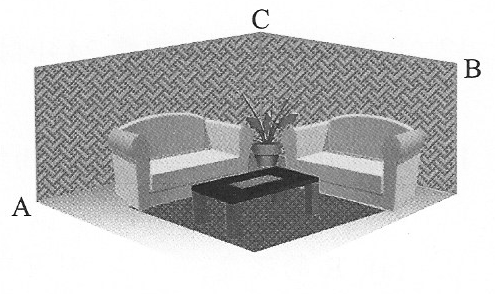
\includegraphics{reception.png}
              \end{center}
              \sol{}
              \begin{center}
                  \begin{tikzpicture}[scale=1.4]
                      \draw (2,1,0) node [above] {$B$} --(0,1,0) node [above] {$C$} --(0,1,2) node [left] {$E$} --(2,1,2)node [above] {$F$} --(2,1,0) --(2,0,0) node [right] {$G$} --(2,0,2) node [below] {$H$}  node [midway, below right] {$6m$} --(0,0,2) node [below] {$A$}  node [midway, below] {$6m$} --(0,1,2);
                      \draw (2,1,2)--(2,0,2);
                      \draw[dashed](2,0,0)--(0,0,0) node [below] {$D$}--(0,1,0);
                      \draw[dashed](0,0,0)--(0,0,2);
                  \end{tikzpicture}
              \end{center}
              \begin{flalign*}
                  \tan{\angle{CAD}} & = \frac{CD}{AD}   \\
                  \tan{30^\circ}    & = \frac{CD}{6}    \\
                  CD                & = 6\tan{30^\circ} \\
                                    & = 2\sqrt{3}m
              \end{flalign*}
              The line connecting $A$ and $B$ with the floor is $\angle BAG$.
              \begin{flalign*}
                  \text{In } ADHG,\ AG & = \sqrt{AH^2 + HG^2} \\
                                       & = \sqrt{6^2 + 6^2}   \\
                                       & = 6\sqrt{2}m
              \end{flalign*}
              \begin{center}
                  \begin{tikzpicture}[scale=1.2]%,cap=round,>=latex]
                      \coordinate [label=left:$A$] (A) at (-1.5cm,-1.cm);
                      \coordinate [label=right:$G$] (C) at (1.5cm,-1.0cm);
                      \coordinate [label=above:$B$] (B) at (1.5cm,1.0cm);
                      \draw (A) -- node[midway,above left] {} (B) -- node[midway, right] {$2\sqrt{3}m$} (C) -- node[below] {$6\sqrt{2}m$} (A);

                      \draw (1.25cm,-1.0cm) rectangle (1.5cm,-0.75cm);
                      \tkzMarkAngle[size=0.5cm,color=black,mark=](C,A,B)
                  \end{tikzpicture}
              \end{center}
              \begin{flalign*}
                  \tan{\angle BAG} & = \frac{BG}{AG}               \\
                                   & = \frac{2\sqrt{3}}{6\sqrt{2}} \\
                  \angle{BAG}      & \approx 22.21^\circ
              \end{flalign*}

        \item The diagram below shows a cuboid with length of $8cm$, width of $5cm$ and
              height of $6cm$, $M$ is the midpoint of $BF$. Find the angle formed by plane
              $HDM$ and plane $ADHE$.
              \begin{center}
                  \begin{tikzpicture}[scale=1.4]
                      \draw (2,1,0) node [above] {$G$} --(0,1,0) node [above] {$H$} --(0,1,2) node [left] {$E$} --(2,1,2)node [above] {$F$} --(2,1,0) --(2,0,0) node [right] {$C$} node [midway, right] {$6cm$} --(2,0,2) node [below] {$B$}  node [midway, below right] {$5cm$} --(0,0,2) node [below] {$A$}  node [midway, below] {$8cm$} --(0,1,2);
                      \draw (2,1,2)--(2,0,2);
                      \draw[dashed](2,0,0)--(0,0,0) node [below] {$D$}--(0,1,0);
                      \draw[dashed](0,0,0)--(0,0,2);
                      \fill [color=gray, opacity=0.4] (0, 1, 0) -- (0, 0, 0) -- (2, 0.5, 2) -- cycle;
                      \draw (2, 0.5, 2) circle (1pt) node [right] {$M$};
                  \end{tikzpicture}
              \end{center}
              \sol{}

              Let the midpoint of $EA$ and $HD$ be $K$ and $L$ respectively.

              $\because$ $HD$ is the common edge of $HDM$ and $ADHE$, $ML \perp HD$, and $KL \perp HD$.

              $\therefore$ The angle formed by plane $HDM$ and plane $ADHE$ is $\angle{MKL}$.
              \begin{center}
                  \begin{tikzpicture}[scale=1.2]%,cap=round,>=latex]
                      \coordinate [label=left:$K$] (A) at (-1.5cm,-1.cm);
                      \coordinate [label=right:$L$] (C) at (1.5cm,-1.0cm);
                      \coordinate [label=above:$M$] (B) at (1.5cm,1.0cm);
                      \draw (A) -- node[midway,above left] {} (B) -- node[midway, right] {$8m$} (C) -- node[below] {$5m$} (A);

                      \draw (1.25cm,-1.0cm) rectangle (1.5cm,-0.75cm);
                      \tkzMarkAngle[size=0.5cm,color=black,mark=](C,A,B)
                  \end{tikzpicture}
              \end{center}
              \begin{flalign*}
                  \tan{\angle MKL} & = \frac{ML}{KL}     \\
                                   & = \frac{8}{5}       \\
                  \angle{MKL}      & \approx 57.99^\circ
              \end{flalign*}

        \item The diagram below shows a pyramid with a square base, its lateral edge $SD$ is
              perpendicular to its base. Given that $BC = 2\sqrt{2}cm$, $SB = 5cm$. Find:
              \begin{center}
                  \begin{tikzpicture}
                      \tikzstyle{point}=[circle,thick,draw=black,fill=black,inner sep=0pt,minimum width=4pt,minimum height=4pt]
                      \node (a) at (0,0) {};
                      \node (b) at (2.5,0) {};
                      \node (c) at (3.5,1) {};
                      \node (d) at (1,1) {};
                      \node (e) at (1,4) {};
                      \draw (a.center) node [below left] {$A$} -- (b.center) node [below] {$B$} -- (c.center) node [ right] {$C$} node [midway, right] {$2\sqrt{2}cm$} -- (e.center) node [above] {$S$} -- (b.center) node [midway, right] {$5cm$};
                      \draw (a.center) -- (e.center);
                      \draw[dashed] (a.center) -- (d.center) -- (c.center);
                      \draw[dashed] (d.center) node [below] {$D$} -- (e.center);
                      \draw (1, 1.25) -- (0.85, 1.1) -- (0.85, 0.85);
                      \draw[dash pattern=on 1pt off 1pt] (d.center) -- (b.center);
                      \fill [fill=gray, opacity=0.4] (d.center) -- (b.center) -- (e.center) -- cycle;
                  \end{tikzpicture}
              \end{center}
              \begin{enumerate}
                  \item The angle formed by plane $SAD$ and plane $SBD$. \sol{}

                        $\because$ $SD$ is the common edge of $SAD$ and $SBD$, $AD \perp SD$, and $BD \perp SD$.

                        $\therefore$ The angle formed by plane $SAD$ and plane $SBD$ is $\angle{ADB}$.
                        \begin{center}
                            \begin{tikzpicture}[scale=1.2]%,cap=round,>=latex]
                                \coordinate [label=left:$D$] (A) at (-1.5cm,-1.cm);
                                \coordinate [label=right:$B$] (C) at (1.5cm,-1.0cm);
                                \coordinate [label=above:$A$] (B) at (1.5cm,1.0cm);
                                \draw (A) -- node[midway,above left] {} (B) -- node[midway, right] {$2\sqrt{2}cm$} (C) -- node[below] {$2\sqrt{2}cm$} (A);

                                \draw (1.25cm,-1.0cm) rectangle (1.5cm,-0.75cm);
                                \tkzMarkAngle[size=0.5cm,color=black,mark=](C,A,B)
                            \end{tikzpicture}
                        \end{center}
                        \begin{flalign*}
                            \tan{\angle ADB} & = \frac{AB}{BD}               \\
                                             & = \frac{2\sqrt{2}}{2\sqrt{2}} \\
                                             & = 1                           \\
                            \angle{ADB}      & = 45^\circ
                        \end{flalign*}

                  \item The angle formed by lateral edge $SA$ and base $ABCD$. \sol{}

                        The angle formed by lateral edge $SA$ and base $ABCD$ is $\angle{SAD}$.
                        \begin{flalign*}
                            \text{In } ABCD,\ DB       & = \sqrt{BC^2 + DC^2}                       \\
                                                       & = \sqrt{{(2\sqrt{2})}^2 + {(2\sqrt{2})}^2} \\
                                                       & = 4cm                                      \\
                            \text{In } \Delta SBD,\ SD & = \sqrt{SB^2 - DB^2}                       \\
                                                       & = \sqrt{5^2 - 4^2}                         \\
                                                       & = 3cm
                        \end{flalign*}
                        \begin{center}
                            \begin{tikzpicture}[scale=1.2]%,cap=round,>=latex]
                                \coordinate [label=left:$A$] (A) at (-1.5cm,-1.cm);
                                \coordinate [label=right:$D$] (C) at (1.5cm,-1.0cm);
                                \coordinate [label=above:$S$] (B) at (1.5cm,1.0cm);
                                \draw (A) -- node[midway,above left] {} (B) -- node[midway, right] {$3cm$} (C) -- node[below] {$2\sqrt{2}cm$} (A);

                                \draw (1.25cm,-1.0cm) rectangle (1.5cm,-0.75cm);
                                \tkzMarkAngle[size=0.5cm,color=black,mark=](C,A,B)
                            \end{tikzpicture}
                        \end{center}
                        \begin{flalign*}
                            \tan{\angle SAD} & = \frac{SD}{AD}       \\
                                             & = \frac{3}{2\sqrt{2}} \\
                            \angle{SAD}      & \approx 46.69^\circ
                        \end{flalign*}
              \end{enumerate}

        \item The diagram below shows a right prism with a rectangular base $ABCD$ with
              length of $28cm$ and width of $20cm$. Assume that plane $VBC$ and the base of
              the pyramid forms a $60^\circ$ angle. Find the angle formed by plane $VAB$ and
              the base.
              \begin{center}
                  \begin{tikzpicture}
                      \tikzstyle{point}=[circle,thick,draw=black,fill=black,inner sep=0pt,minimum width=4pt,minimum height=4pt]
                      \node (a) at (0,0) {};
                      \node (b) at (2.5,0) {};
                      \node (c) at (3.5,1) {};
                      \node (d) at (1,1) {};
                      \node (e) at (1.75,3) {};
                      \draw (a.center) node [below left] {$A$} -- (b.center) node [below] {$B$} node [midway, below] {$28cm$} -- (c.center) node [ right] {$C$} node [midway, right=12pt, below=-4pt] {$20cm$} -- (e.center) node [above] {$V$} -- (b.center);
                      \draw (a.center) -- (e.center);
                      \draw[dashed] (a.center) -- (d.center) -- (c.center);
                      \draw[dashed] (d.center) node [below] {$D$} -- (e.center);
                  \end{tikzpicture}
              \end{center}
              \sol{}

              Let the footpoint of $V$ be $M$, and the midpoint of $AB$ and $BC$ be $E$ and
              $F$ respectively.

              $\because$ $BC$ is the common edge of $VBC$ and $ABCD$, $VF \perp BC$, and $MF \perp BC$.

              $\therefore$ The angle formed by plane $VBC$ and the base is $\angle{VFM}$.

              Given that $VFM = 60^\circ$,
              \begin{flalign*}
                  \tan{\angle VFM} & = \frac{VM}{MF}           \\
                  \tan{60^\circ}   & = \frac{VM}{\frac{AB}{2}} \\
                                   & = \frac{VM}{14}           \\
                  VM               & = 14\sqrt{3}cm
              \end{flalign*}

              $\because$ $VE$ is the common edge of $VAB$ and $ABCD$, $VE \perp AB$, and $ME \perp AB$.

              $\therefore$ The angle formed by plane $VAB$ and the base is $\angle{VEM}$.
              \begin{center}
                  \begin{tikzpicture}[scale=1.2]%,cap=round,>=latex]
                      \coordinate [label=left:$E$] (A) at (-1.5cm,-1.cm);
                      \coordinate [label=right:$M$] (C) at (1.5cm,-1.0cm);
                      \coordinate [label=above:$V$] (B) at (1.5cm,1.0cm);
                      \draw (A) -- node[midway,above left] {} (B) -- node[midway, right] {$14\sqrt{3}cm$} (C) -- node[below] {$10cm$} (A);

                      \draw (1.25cm,-1.0cm) rectangle (1.5cm,-0.75cm);
                      \tkzMarkAngle[size=0.5cm,color=black,mark=](C,A,B)
                  \end{tikzpicture}
                  \begin{flalign*}
                      \tan{\angle VEM} & = \frac{VM}{ME}         \\
                                       & = \frac{14\sqrt{3}}{10} \\
                      \angle{VEM}      & \approx 67.59^\circ
                  \end{flalign*}
              \end{center}

        \item The diagram below shows a regular cuboid with a square base. Given that $VE =
                  \frac{5}{2}AD$. Find:
              \begin{center}
                  \begin{tikzpicture}
                      \tikzstyle{point}=[circle,thick,draw=black,fill=black,inner sep=0pt,minimum width=4pt,minimum height=4pt]
                      \node (a) at (0,0) {};
                      \node (b) at (2.5,0) {};
                      \node (c) at (3.5,1) {};
                      \node (d) at (1,1) {};
                      \node (e) at (1.75,5) {};
                      \draw (a.center) node [below left] {$A$} -- (b.center) node [below] {$B$} -- (c.center) node [ right] {$C$} -- (e.center) node [above] {$V$} -- (b.center);
                      \draw (a.center) -- (e.center);
                      \draw[dashed] (a.center) -- (d.center) -- (c.center);
                      \draw[dashed] (d.center) node [below] {$D$} -- (e.center);
                      \node (f) at (1.75, 0.5) {};
                      \draw[dash pattern=on 1pt off 1pt] (e.center) -- (f.center);
                      \draw[dash pattern=on 1pt off 1pt] (a.center) -- (c.center);
                      \draw[dash pattern=on 1pt off 1pt] (b.center) -- (d.center) node [midway, below] {$E$};
                  \end{tikzpicture}
              \end{center}
              \begin{enumerate}
                  \item The angle formed by the angle $VA$ and the base $ABCD$. \sol{}

                        Let $AD$ be $2\ units$, then $VE = \frac{5}{2}AD = 5\ units$.

                        The angle formed by the angle $VA$ and the base $ABCD$ is $VAE$.
                        \begin{flalign*}
                            \text{In } ABCD, AC & = \sqrt{AD^2 + DC^2} \\
                                                & = \sqrt{2^2 + 2^2}   \\
                                                & = 2\sqrt{2}\ units   \\
                            AE                  & = \frac{1}{2}AC      \\
                                                & = \sqrt{2}\ units
                        \end{flalign*}
                        \begin{center}
                            \begin{tikzpicture}[scale=1.2]%,cap=round,>=latex]
                                \coordinate [label=left:$A$] (A) at (-1.5cm,-1.cm);
                                \coordinate [label=right:$E$] (C) at (1.5cm,-1.0cm);
                                \coordinate [label=above:$V$] (B) at (1.5cm,1.0cm);
                                \draw (A) -- node[midway,above left] {} (B) -- node[midway, right] {$5\ units$} (C) -- node[below] {$\sqrt{2}\ units$} (A);

                                \draw (1.25cm,-1.0cm) rectangle (1.5cm,-0.75cm);
                                \tkzMarkAngle[size=0.5cm,color=black,mark=](C,A,B)
                            \end{tikzpicture}
                        \end{center}
                        \begin{flalign*}
                            \tan{\angle VAE} & = \frac{VE}{AE}      \\
                                             & = \frac{5}{\sqrt{2}} \\
                            \angle VAE       & \approx 74.21^\circ
                        \end{flalign*}

                  \item The angle formed by plane $VAD$ and the base. \sol{}

                        Let $M$ be the midpoint of $AD$.

                        $\because$ $AD$ is the common edge of $ABCD$ and $VAD$, $ME \perp AD$, and $VE \perp AD$.

                        $\therefore$ The angle formed by plane $VAD$ and the base is $VME$.
                        \begin{center}
                            \begin{tikzpicture}[scale=1.2]%,cap=round,>=latex]
                                \coordinate [label=left:$M$] (A) at (-1.5cm,-1.cm);
                                \coordinate [label=right:$E$] (C) at (1.5cm,-1.0cm);
                                \coordinate [label=above:$V$] (B) at (1.5cm,1.0cm);
                                \draw (A) -- node[midway,above left] {} (B) -- node[midway, right] {$5\ units$} (C) -- node[below] {$1\ units$} (A);

                                \draw (1.25cm,-1.0cm) rectangle (1.5cm,-0.75cm);
                                \tkzMarkAngle[size=0.5cm,color=black,mark=](C,A,B)
                            \end{tikzpicture}
                        \end{center}
                        \begin{flalign*}
                            \tan{\angle VME} & = \frac{VE}{ME}     \\
                                             & = \frac{5}{1}       \\
                                             & = 5                 \\
                            \angle VME       & \approx 78.69^\circ
                        \end{flalign*}
              \end{enumerate}

        \item Find the distance from the Panama City$(9^\circ N, 79^\circ 30' W)$ to Toronto
              $(43^\circ 45' N, 79^\circ 30' W)$. (Express your answer in nautical miles)
              \sol{}
              \begin{flalign*}
                  \overset{\frown}{PT} & = (43^\circ 45' - 9^\circ) \times 60 \\
                                       & = 34^\circ 45' \times 60             \\
                                       & = 2085\text{\emph{NM}}
              \end{flalign*}

        \item Tokyo and Adelaide are located at the same longitude, their latitude are
              $35^\circ 45' N$ and $35^\circ S$ respectively. Find the distance between two
              cities along the parallel of latitude. \sol{}
              \begin{flalign*}
                  \overset{\frown}{TA} & = (35^\circ 45' + 35^\circ) \times 60 \\
                                       & = 70^\circ 45' \times 60              \\
                                       & = 4245\text{\emph{NM}}                \\
                                       & = 4245 \times 1.853km                 \\
                                       & = 7,865.99km
              \end{flalign*}

        \item A plane flies $2000$\emph{NM} along the equator, Find the difference of
              longitude between the point of departure and the destination. \sol{}
              \begin{flalign*}
                  d      & = \alpha \times 60 \times \cos{0} \\
                  2000   & = \alpha \times 60 \times 1       \\
                  \alpha & = \frac{2000}{60}                 \\
                         & = 33.33^\circ
              \end{flalign*}

        \item Location $M$ and $N$ are both located at the parallel of latitude $45^\circ$
              north to the equator with a difference in longitude of $20^\circ$. Find the
              distance between $M$ and $N$ along the parallel of latitude. (Express your
              answer in nautical miles) \sol{}
              \begin{flalign*}
                  \overset{\frown}{MN} & = 20^\circ \times 60 \times \cos{45^\circ} \\
                                       & = 848.53\text{\emph{NM}}
              \end{flalign*}

        \item Location $X$ and $Y$ are on the parallel of latitude $20^\circ$ north to the
              equator, their longitude are $45^\circ E$ and $80^\circ E$ respectively. Find
              the distance between location $X$ and $Y$ along the parallel of latitude.
              (Express your answer in nautical miles) \sol{}
              \begin{flalign*}
                  \overset{\frown}{XY} & = (80^\circ - 45^\circ) \times 60 \times \cos{20^\circ} \\
                                       & = 35^\circ \times 60 \times \cos{20^\circ}              \\
                                       & = 1973.35\text{\emph{NM}}
              \end{flalign*}

        \item A plane flies from $A(42^\circ E)$ to $B(20^\circ E)$ along the equator, then
              it flies from $B$ due north to $C(30^\circ N)$. Find the distance the plane
              flies in total. \sol{}
              \begin{flalign*}
                  \overset{\frown}{AB} & = (42^\circ - 20^\circ) \times 60 \times \cos{0} \\
                                       & = 22^\circ \times 60 \times 1                    \\
                                       & = 1320\text{\emph{NM}}                           \\
                  \overset{\frown}{BC} & = (30^\circ - 0^\circ) \times 60                 \\
                                       & = 1800\text{\emph{NM}}                           \\
                  d                    & = \overset{\frown}{AB} + \overset{\frown}{BC}    \\
                                       & = 1320\text{\emph{NM}} + 1800\text{\emph{NM}}    \\
                                       & = 3120\text{\emph{NM}}
              \end{flalign*}
        \item Assume that $A$ is located $1000$\emph{NM} due north of the equator,
              $600$\emph{NM} due east of the Greenwich Meridian, find the longitude and
              latitude of $A$.
              \begin{flalign*}
                  \overset{\frown}{AE} & = \frac{1000}{60}                            \\
                                       & = 16^\circ 40'                               \\
                  \text{Lat.} A        & = 16^\circ 40' N                             \\
                  \overset{\frown}{AG} & = \alpha \times 60 \times \cos{16^\circ 40'} \\
                  600                  & = \alpha \times 60 \times \cos{16^\circ 40'} \\
                  \alpha               & = \frac{600}{60 \times \cos{16^\circ 40' N}} \\
                                       & = 10^\circ 26'                               \\
                  \text{Lon.} A        & = 10^\circ 26' E
                  \\
                  \therefore\ A        & (16^\circ 40' N, 10^\circ 26' E)
              \end{flalign*}

        \item A plane flies from $P(15^\circ N, 30^\circ E)$ $2000$\emph{NM} due south to
              $B$, find the longitude and latitude of $B$. Another plane flies from $P$
              $3000$\emph{NM} due east to $C$, find the longitude and latitude of $C$.
              \begin{flalign*}
                  \overset{\frown}{PB} & = \frac{2000}{60}                        \\
                                       & = 33^\circ 20'                           \\
                  \text{Lat.} B        & = |15^\circ N - 33^\circ 20'|S           \\
                                       & = 18^\circ 20' S                         \\
                  \\
                  \therefore\ B        & (18^\circ 20' S, 30^\circ E)             \\
                  \\
                  \overset{\frown}{PC} & = \alpha \times 60 \times \cos{15^\circ} \\
                  3000                 & = \alpha \times 60 \times \cos{15^\circ} \\
                  \alpha               & = \frac{3000}{60 \times \cos{15^\circ}}  \\
                                       & = 51^\circ 46'                           \\
                  \text{Lon.} C        & = (30^\circ + 51^\circ 46')E             \\
                                       & = 81^\circ 46' E                         \\
                  \\
                  \therefore\ C        & (15^\circ N, 81^\circ 46' E)
              \end{flalign*}

        \item A plane flies from $A(130^\circ E)$ along the equator to $B(120^\circ 30' E)$
              along the equator, then flies from $B$ due north to $C(20^\circ 45')$. Assume
              that the average speed of the plane is $300\text{\emph{NM}}/hr$ throughout the
              journey, find the flight duration for the whole journey. \sol{}
              \begin{flalign*}
                  \overset{\frown}{AB} & = (130^\circ - 120^\circ 30') \times 60 \times \cos{0} \\
                                       & = 9^\circ 30' \times 60 \times 1                       \\
                                       & = 570\text{\emph{NM}}                                  \\
                  \overset{\frown}{BC} & = (20^\circ 45' - 0^\circ) \times 60                   \\
                                       & = 1245\text{\emph{NM}}                                 \\
                  d                    & = \overset{\frown}{AB} + \overset{\frown}{BC}          \\
                                       & = 570\text{\emph{NM}} + 1245\text{\emph{NM}}           \\
                                       & = 1815\text{\emph{NM}}                                 \\
                  t                    & = \frac{1815\text{\emph{NM}}}{300\text{\emph{NM}}/hr}  \\
                                       & = 6.05\text{\emph{hrs}}                                \\
                                       & = 6\text{\emph{hrs}}\ 3\text{\emph{mins}}
              \end{flalign*}
        \item A plane flies from $A(50^\circ N, 10^\circ E)$ due east to $B(45^\circ E)$.
              \begin{enumerate}
                  \item Find the flight distance of the plane. (Express your answer in nautical miles)
                        \sol{}
                        \begin{flalign*}
                            \overset{\frown}{AB} & = (45^\circ - 10^\circ) \times 60 \times \cos{50^\circ} \\
                                                 & = 35^\circ \times 60 \times \cos{50^\circ}              \\
                                                 & = 1349.85\text{\emph{NM}}                               \\
                        \end{flalign*}

                  \item Assume that the speed of the plane is $420\text{\emph{NM}}/hr$ in average, find
                        the flight duration of the plane. \sol{}
                        \begin{flalign*}
                            t & = \frac{1349.85\text{\emph{NM}}}{420\text{\emph{NM}}/hr} \\
                              & = 3\text{\emph{hrs}}\ 13\text{\emph{mins}}
                        \end{flalign*}
              \end{enumerate}
        \item Given that three locations $P$, $Q$ and $R$ are located on the same parallel of
              latitude $40^\circ$ north to the equator, The longitude of $P$ and $R$ are
              $10^\circ 30' W$ and $4^\circ 30' E$, $Q$ is located at the middle of $P$ and
              $R$.
              \begin{enumerate}
                  \item Find the difference of longitude between $P$ and $R$. \sol{}
                        \begin{flalign*}
                            \overset{\frown}{PR} & = 10^\circ 30' + 4^\circ 30' \\
                                                 & = 15^\circ
                        \end{flalign*}

                  \item Find the longitude of $Q$. \sol{}
                        \begin{flalign*}
                            \overset{\frown}{PQ} & = \frac{\overset{\frown}{PR}}{2}                         \\
                                                 & = 344.72\text{\emph{NM}}                                 \\
                            \text{Lon.} Q        & = 10^\circ 30' + \frac{344.72}{60 \times \cos{40^\circ}} \\
                                                 & = 10^\circ 30' - 7^\circ 30'                             \\
                                                 & = 3^\circ W
                        \end{flalign*}

                  \item Find the distance between $P$ and $R$ along the parallel of latitude.
                        \begin{flalign*}
                            \overset{\frown}{PR} & = 15^\circ \times 60 \times \cos{40^\circ} \\
                                                 & = 689.44\text{\emph{NM}}
                        \end{flalign*}
                  \item A ship sails from $P$ to $Q$ along the parallel of latitude with a speed of
                        $18\text{\emph{NM}}/hr$, find the sailing duration of the ship.
                        \begin{flalign*}
                            t & = \frac{344.72\text{\emph{NM}}}{18\text{\emph{NM}}/hr} \\
                              & = 19hrs\ 9mins
                        \end{flalign*}
              \end{enumerate}
    \end{enumerate}

\end{multicols}
\end{document}